% Escolha: Portugues ou Ingles ou Espanhol.
% Para a versão final do texto, após a defesa, acrescente Final:

\documentclass[Portugues]{ic-tese-v3}
% \documentclass[Portugues,Final]{ic-tese-v3}

\usepackage[latin1,utf8]{inputenc}
\usepackage[brazil]{babel}

% Para acrescentar comentários ao PDF descomente:
\usepackage
 % [pdfauthor={nome do autor},
  % pdftitle={titulo},
%   pdfkeywords={palavra-chave, palavra-chave},
%   pdfproducer={Latex with hyperref},
%   pdfcreator={pdflatex}]
{hyperref}
\usepackage{cite}

\usepackage{graphicx}

\usepackage{xcolor}
\newcommand{\todo}[1]{{\color{red}{\large TODO:} #1}}

\usepackage[portugues, vlined, noend, ruled, linesnumbered]{algorithm2e}

\usepackage{multirow}
\usepackage{enumerate}

\usepackage{amsfonts}
\usepackage{amssymb}
\usepackage{amsthm}
\usepackage{amsmath}

\newtheorem{theorem}{Teorema}[section]
\newtheorem{corollary}{Corolário}[theorem]
\newtheorem{lemma}[theorem]{Lema}

\theoremstyle{definition}
\newtheorem{definition}{Definição}[section]

\theoremstyle{remark}
\newtheorem{remark}{Observação}[section]

\theoremstyle{definition}
\newtheorem{example}{Exemplo}[section]

\newcommand{\position}{center}

% Classic
\newcommand{\SbR}{\textbf{SbR}}
\newcommand{\SbT}{\textbf{SbT}}
\newcommand{\SbBI}{\textbf{SbBI}}
\newcommand{\SbRT}{\textbf{SbRT}}
% Weighted
\newcommand{\SbWRT}{\textbf{Sb\textsubscript{W}RT}}
\newcommand{\SbWRTIT}{\textbf{Sb\textsubscript{W}RTIT}}
\newcommand{\SbWIRI}{\textbf{Sb\textsubscript{WI}RI}}
\newcommand{\SbWIRTI}{\textbf{Sb\textsubscript{WI}RTI}}
\newcommand{\SbWIRT}{\textbf{Sb\textsubscript{WI}RT}}
% Proportion
\newcommand{\SbPRT}{\textbf{Sb\textsubscript{P}RT}}
% Intergenic
\newcommand{\SbIBI}{\textbf{Sb\textsubscript{I}BI}}
\newcommand{\SbIR}{\textbf{Sb\textsubscript{I}R}}
\newcommand{\SbIRI}{\textbf{Sb\textsubscript{I}RI}}
\newcommand{\SbIRM}{\textbf{Sb\textsubscript{I}RM}}
\newcommand{\SbIRMI}{\textbf{Sb\textsubscript{I}RMI}}
\newcommand{\SbIT}{\textbf{Sb\textsubscript{I}T}}
\newcommand{\SbITM}{\textbf{Sb\textsubscript{I}TM}}
\newcommand{\SbIRT}{\textbf{Sb\textsubscript{I}RT}}
\newcommand{\SbIRTI}{\textbf{Sb\textsubscript{I}RTI}}
\newcommand{\SbIRTM}{\textbf{Sb\textsubscript{I}RTM}}
\newcommand{\SbIRTMI}{\textbf{Sb\textsubscript{I}RTMI}}
% Flexible
\newcommand{\SbFIR}{\textbf{Sb\textsubscript{FI}R}}
\newcommand{\SbFIRI}{\textbf{Sb\textsubscript{FI}RI}}
\newcommand{\SbFIRM}{\textbf{Sb\textsubscript{FI}RM}}
\newcommand{\SbFIRMI}{\textbf{Sb\textsubscript{FI}RMI}}
\newcommand{\SbFIT}{\textbf{Sb\textsubscript{FI}T}}
\newcommand{\SbFITM}{\textbf{Sb\textsubscript{FI}TM}}
\newcommand{\SbFIRT}{\textbf{Sb\textsubscript{FI}RT}}
\newcommand{\SbFIRTI}{\textbf{Sb\textsubscript{FI}RTI}}
\newcommand{\SbFIRTM}{\textbf{Sb\textsubscript{FI}RTM}}
\newcommand{\SbFIRTMI}{\textbf{Sb\textsubscript{FI}RTMI}}

\usepackage{environ}

\makeatletter
\newcommand{\problemtitle}[1]{\gdef\@problemtitle{#1}}% Store problem title
\newcommand{\probleminput}[1]{\gdef\@probleminput{#1}}% Store problem input
\newcommand{\problemtask}[1]{\gdef\@problemtask{#1}}% Store problem task
\newcommand{\problemquestion}[1]{\gdef\@problemquestion{#1}}% Store problem question

% Problem task enviroment
\NewEnviron{task}{
  \problemtitle{}\probleminput{}\problemtask{}% Default input is empty
  \BODY
  \begin{center}
  \fbox{
    \begin{minipage}{0.9\linewidth}
      \raggedright
      \parskip=1ex
      \textbf{\@problemtitle}          \\% Title
      \textbf{Entrada:} \@probleminput \\% Input
      \textbf{Objetivo:} \@problemtask \\% Goal
    \end{minipage}
  } 
  \end{center}
}
\NewEnviron{decision}{
  \problemtitle{}\probleminput{}\problemquestion{}% Default input is empty
  \BODY
  \begin{center}
  \fbox{
    \begin{minipage}{0.9\linewidth}
      \raggedright
      \parskip=1ex
      \@problemtitle                   \\% Title
      \textbf{Entrada:} \@probleminput \\% Input
      \textbf{Pergunta:} \@problemquestion \\% Goal
    \end{minipage}
  } 
  \end{center}
}
\makeatother

\usepackage{tikz}
\usetikzlibrary{arrows}
\usetikzlibrary{arrows.meta}
\usetikzlibrary{positioning, shapes.arrows, shapes.geometric, shapes.misc, backgrounds}
\usetikzlibrary{fit}

\tikzset{ 
signed gene/.style = { single arrow, draw = black, fill = white, minimum size = 10mm, single arrow head extend = 1mm },
unsigned gene/.style = { circle, draw = black, fill = white, minimum size = 10mm },
ir/.style = { rectangle, draw = black, fill = white, minimum size = 10mm, rounded corners = 5pt},
}


\tikzset{
pics/right gene/.style args={#1, #2}{
        code = {
        % \path[draw = black, fill = #2] (0.5, 0.0) -- (0.3, -0.5) -- (-0.5, -0.5) -- (-0.3, 0.0) -- (-0.5, 0.5) -- (0.3, 0.5) -- cycle;
        \path[draw = black, fill = #2] (0.5, 0.0) -- (0.3, -0.5) -- (-0.5, -0.5) -- (-0.5, 0.5) -- (0.3, 0.5) -- cycle;
        \node[black, draw = none, fill = none, minimum size = 10mm] at (0.0, 0.0) {#1};
        }
    },
pics/left gene/.style args={#1, #2}{
        code = {
        % \path[draw = black, fill = #2] (-0.5, 0.0) -- (-0.3, 0.5) -- (0.5, 0.5) -- (0.3, 0.0) -- (0.5, -0.5) -- (-0.3, -0.5) -- cycle;
        \path[draw = black, fill = #2] (-0.5, 0.0) -- (-0.3, 0.5) -- (0.5, 0.5) -- (0.5, -0.5) -- (-0.3, -0.5) -- cycle;
        \node[black, draw = none, fill = none, minimum size = 10mm] at (0.0, 0.0) {#1};
        }
    },
pics/gene/.style args={#1, #2}{
        code = {
        \node[black, circle, draw = black, fill = #2, minimum size = 10mm] at (0.0, 0.0) {#1};
        }
    },
pics/ir/.style args={#1, #2}{
        code = {
        \node[rectangle, draw = black, fill = #2, minimum size = 10mm, rounded corners = 5pt] at (0.0, 0.0) {#1};
        }
    },
pics/flex ir/.style args={#1, #2, #3}{
        code = {
        \node[rectangle, draw = black, fill = #3, minimum size = 10mm, rounded corners = 5pt] at (0.0, 0.0) {};
        \node [black] at (0.0, 0.25) {#2};
        \node [black] at (0.0, -0.25) {#1};
        }
    }
}




\begin{document}

% Escolha entre autor ou autora:
\autor{Klairton de Lima Brito}
%\autora{Nome da Autora}

% Sempre deve haver um título em português:
\titulo{Modelos com Proporção entre Operações e Regiões Intergênicas Rígidas e Flexíveis}

% Se a língua for o inglês ou o espanhol defina:
\title{Models with a Proportion Ratio between Operations and Rigid and Flexible Intergenic Regions}

% Escolha entre orientador ou orientadora. Inclua os títulos acadêmicos:
\orientador{Prof. Dr. Zanoni Dias}
%\orientadora{Profa. Dra. Nome da Orientadora}

% Escolha entre coorientador ou coorientadora, se houver.  Inclua os títulos acadêmicos:
\coorientador{Prof. Dr. Ulisses Martins Dias}
%\coorientadora{Profa. Dra. Eng. Lic. Nome da Co-Orientadora}

% Escolha entre mestrado ou doutorado:
% \mestrado
\doutorado

% Se houve cotutela, defina:
%\cotutela{Universidade Nova de Plutão}

\datadadefesa{16}{12}{2022}

% Para a versão final defina:
\avaliadorA{Prof. Dr. Zanoni Dias}{Universidade Estadual de Campinas}
\avaliadorB{Profa. Dra. Carla Negri Lintzmayer}{Universidade Federal do ABC}
\avaliadorC{Profa. Dra. Maria Emília Machado Telles Walter}{Universidade de Brasília}
\avaliadorD{Prof. Dr. Orlando Lee}{Universidade Estadual de Campinas}
\avaliadorE{Prof. Dr. Rafael Crivellari Saliba Schouery}{Universidade Estadual de Campinas}
%\avaliadorF{Prof. Dr. Sexto Avaliador}{Instituição do sexto avaliador}
%\avaliadorG{Prof. Dr. Sétimo Avaliador}{Instituição do sétimo avaliador}
%\avaliadorH{Prof. Dr. Oitavo Avaliador}{Instituição do oitavo avaliador}


% Para incluir a ficha catalográfica em PDF na versão final, descomente e ajuste:
%\fichacatalografica{arquivo.pdf}


% Este comando deve ficar aqui:
\paginasiniciais


% Se houver dedicatória, descomente:
%\prefacesection{Dedicatória}
%A dedicatória deve ocupar uma única página.


% Se houver epígrafe, descomente e edite:
% \begin{epigrafe}
% {\it
% Vita brevis,\\
% ars longa,\\
% occasio praeceps,\\
% experimentum periculosum,\\
% iudicium difficile.}
%
% \hfill (Hippocrates)
% \end{epigrafe}


% Agradecimentos ou Acknowledgements ou Agradecimientos
\prefacesection{Agradecimentos}
Esta tese foi realizada com apoio da Coordenação de Aperfeiçoamento de Pessoal de Nível Superior - Brasil (CAPES) - Código de Financiamento 001, do Conselho Nacional de Desenvolvimento Científico e Tecnológico - (CNPq) - Processo 140272/2020-8, e do acordo CAPES/COFECUB - Projeto 831/15 - Processo 88887.185411/2018-00.

% Sempre deve haver um resumo em português:
\begin{resumo}
A genômica comparativa é um campo de pesquisa da biologia com foco na comparação de características genéticas entre organismos. Dentre as características genéticas comumente utilizadas, podemos citar a sequência de genes dos genomas. O número de mutações genéticas capazes de transformar uma sequência genética em outra é uma das métrica de comparação amplamente utilizada para a comparação de dois genomas. Os eventos de rearranjo de genoma são eventos mutacionais que podem afetar grandes trechos de um genoma. A reversão e a transposição são dois dos eventos de rearranjo mais estudados na literatura. Uma reversão inverte um segmento do genoma, enquanto uma transposição troca a posição de dois segmentos adjacentes.

Um modelo de rearranjo determina o conjunto de eventos de rearranjo que podem ser utilizados para transformar um genoma em outro. Os primeiros estudos apresentaram resultados considerando um modelo de rearranjo constituído exclusivamente por um único tipo de evento de rearranjo. No entanto, estudos posteriores apresentaram resultados considerando modelos de rearranjo compostos por múltiplos eventos de rearranjo. Quando consideramos apenas o número de eventos de rearranjo necessários para transformar um genoma em outro, assumimos que cada evento tem a mesma probabilidade de ocorrer em um cenário evolutivo, sendo essa abordagem chamada de não ponderada. No entanto, quando desejamos que determinados tipos de eventos ocorram mais do que outros, é possível atribuir um custo a cada tipo de evento de rearranjo. Nessa nova versão, o objetivo do problema consiste em buscar uma sequência de eventos de rearranjo que transforme um genoma em outro com custo mínimo, sendo essa abordagem chamada de ponderada. Nesta tese, apresentamos uma abordagem que considera uma proporção mínima entre a quantidade de eventos de reversão e o tamanho da sequência de eventos de rearranjo que transforma um genoma em outro. Nós mostramos que a abordagem de proporção naturalmente contorna problemas que podem surgir adotando uma abordagem ponderada ou não ponderada. Além disso, realizamos uma análise de complexidade do problema e apresentamos algoritmos de aproximação com fatores constantes.

Estudos têm destacado a importância da informação presente nas regiões intergênicas, que são estruturas presentes entre cada par de genes e nas extremidades de um genoma, e que podem levar a modelos mais realistas considerando um contexto evolutivo. O tamanho de cada região intergênica é dado pelo número de nucleotídeos presente nela. Desde então, foram apresentados estudos considerando tanto a sequência de genes quanto o tamanho das regiões intergênicas para representar um genoma. Nesta tese, mostramos resultados nesse mesmo contexto, mas consideramos diferentes modelos de rearranjo. Além disso, introduzimos uma generalização dos problemas possibilitando atribuir um grau de flexibilidade em relação ao tamanho das regiões intergênicas desejadas no genoma alvo. Para ambos os casos, realizamos uma análise de complexidade dos problemas, desenvolvemos algoritmos e conduzimos experimentos para verificar o desempenho prático. 
\end{resumo}


% Sempre deve haver um abstract:
\begin{abstract}

Comparative genomics is a field of research in biology focusing on comparing genetic features between organisms. Among the genetic features commonly used, we can mention the sequence of genes in genomes. The number of genetic mutations capable of transforming one gene sequence into another is a widely used metric to compare genomes. Genome rearrangement events are mutational events that can affect large stretches of a genome. Reversal and transposition are two of the most studied rearrangement events in the literature. A reversal inverts a genome segment, while a transposition exchanges the position of two adjacent segments.

A rearrangement model determines the set of rearrangement events that can be used to transform one genome into another. Early studies presented results considering a rearrangement model consisting exclusively of a single type of rearrangement event. However, subsequent studies presented results considering rearrangement models composed of multiple rearrangement events. When we consider only the number of rearrangement events that are required to transform one genome into another, we assume that each event has the same probability of occurring in an evolutionary scenario; this is called the unweighted approach. However, when we want certain types of events to occur more than others, it is possible to assign a cost to each type of rearrangement event. The problem goal changes to search for a sequence of rearrangement events that transforms one genome into another with minimal cost; this is called the weighted approach. In this work, we introduce an approach that considers a minimum proportion between the number of reversal events and the size of the rearrangement sequence that transforms one genome into another. We show that the proportion approach naturally overcomes problems that may arise by adopting a weighted or unweighted approach. In addition, we perform a complexity analysis of the problem and present approximation algorithms with constant factors.

Another genetic feature that studies pointed out as relevant in a genetic comparison context is the intergenic regions, which are structures between each pair of genes and at the extremities of a genome. The size of each intergenic region is the number of nucleotides within it. Since then, studies were presented considering both the sequence of genes and the size of the intergenic regions to represent a genome. In this work, we show results in this same context but we consider different rearrangement models. In addition, we introduce a generalization of the problems such that it is possible to assign a degree of flexibility regarding the size of the intergenic regions desired in the target genome. For both cases, we conducted a complexity analysis of the problems, developed algorithms, and performed experiments to verify the practical performance.
\end{abstract}


% Se houver um resumo em espanhol, descomente:
%\begin{resumen}
% A mesma regra aplica-se.
%\end{resumen}


% A lista de figuras é opcional:
\listoffigures

% A lista de tabelas é opcional:
\listoftables

% A lista de abreviações e siglas é opcional:
% \prefacesection{Lista de Abreviações e Siglas}

% A lista de símbolos é opcional:
% \prefacesection{Lista de Símbolos}

% Quem usa o pacote nomencl pode incluir:
%\renewcommand{\nomname}{Lista de Abreviações e Siglas}
%\printnomenclature[3cm]


% O sumário vem aqui:
% \setcounter{tocdepth}{3}
\tableofcontents


% E esta linha deve ficar bem aqui:
\fimdaspaginasiniciais


% O corpo da dissertação ou tese começa aqui:
\chapter{Introdução}\label{chapter:XDSEJBWV}
\chapter{Introdução}\label{chapter:XDSEJBWV}

O estudo da evolução dos organismos é uma tarefa de fundamental importância no campo da biologia. Ao decorrer do tempo mudanças podem ocorrer nos organismos, que refletem adaptações desenvolvidas para melhor se adequar e prosperar no ambiente que estão inseridos. Em particular, mudanças genéticas são uma das características utilizadas no campo da \emph{genômica comparativa} para estimar a proximidade de dois organismos com base na similaridade de seus materiais genéticos. O genoma pode sofrer modificações a partir de mutações que podem ser pontuais ou afetar grandes trechos do genoma, que são chamadas de eventos de rearrajos de genomas. Tais eventos podem afetar o genoma modificando, inserindo ou removendo material genético~\cite{2009-fertin-etal}. Uma das formas bem aceita de estimar a proximidade de dois organismos é determinando uma sequência de eventos de rearranjos de genomas com tamanho mínimo e capaz de transformar o genoma de um organismo em outro. O tamanho de tal sequência é chamada de \emph{distância de rearranjo}.

Reversão e transposição são os eventos de rearranjo mais estudados na literatura~\cite{1999-hannenhalli-pevzner,1999-caprara,2012-bulteau-etal,2019b-oliveira-etal}. Uma reversão atua em um segmento do genoma invertendo a posição e a orientação dos genes contidos no segmento, enquanto uma transposição troca dois segmentos consecutivos do genoma, mas sem afetar a posição e a orientação dos genes nos segmentos. Os eventos de reversão e transposição são chamados de conservativos, pois não alteram a quantidade de material genético do genoma. Existem também eventos não conservativos, como é o caso dos eventos de inserção, deleção e duplicação~\cite{2013-willing-etal,2012-elmabrouk-sankoff,2008-kahn-raphael,2020-mane-etal,2009-bader}, que inserem, removem e duplicam material genético de uma região específica do genoma, respectivamente. Um modelo de rearranjo é caracterizado pelo conjunto de eventos de rearranjo permitidos para transformar um genoma em outro.

Um genoma pode ser representado computacionalmente de diferentes maneiras. Quan\-do o genoma é tratado como uma sequência ordenada de genes, podemos encontrar casos em que determinados genes apresentam múltiplas cópias, sendo comum utilizarmos uma representação na forma de uma cadeia de caracteres (strings), onde cada caractere é associado a um gene. Por outro lado, se existir apenas uma cópia de cada gene, podemos associar um número inteiro para cada gene e a representação é dada na forma de uma permutação. Em ambos os casos, quando a orientação dos genes é conhecida, um sinal de positivo ou negativo é atribuído para cada elemento e a representação é chamada com sinais (string com sinais e permutação com sinais). Caso contrário, o sinal é omitido e a representação é chamada sem sinais (string sem sinais e permutação sem sinais). Chamamos a representação de um genoma através de uma permutação de representação clássica e a representação de um genoma por meio de uma string por representação por strings.

Ao utilizar a representação clássica, podemos simplificar o problema como sendo um problema de ordenação. Nesse caso, o objetivo consiste em transformar uma permutação $\pi$ qualquer em uma permutação específica na qual os elementos encontram-se ordenados de maneira crescente e com sinal positivo para o caso com sinais, essa permutação é chamada de identidade.

Quando consideramos um modelo de rearranjo composto apenas pelo evento de reversão e utilizando uma representação clássica com sinais, temos a variação com sinais do problema de Ordenação de Permutações por Reversões (\SbR). Hannenhalli e Pevzner~\cite{1999-hannenhalli-pevzner} apresentaram o primeiro algoritmo exato polinomial para o problema, sendo posteriormente simplificado por Bergeron~\cite{2005-bergeron}. Atualmente, temos um algoritmo com complexidade subquadrática para determinar a sequência de reversões capaz de ordenar uma permutação com sinais~\cite{2007-tannier-etal}. Entretanto, se estivermos interessados somente na distância de reversão, existe um algoritmo que executa em tempo linear~\cite{2001-bader-etal}. Quando consideramos uma representação clássica sem sinais, temos a variação sem sinais do problema \SbR. Caprara~\cite{1999-caprara} provou que o problema faz parte da classe de problemas NP-Difícil. Um dos primeiros algoritmos para o problema apresentou um fator de aproximação $1.75$~\cite{1996-bafna-pevzner}. Em seguida, Christie~\cite{1998a-christie} apresentou um algoritmo com fator de aproximação $1.5$. Atualmente, o melhor algoritmo para o problema apresenta um fator de aproximação $1.375$~\cite{2002-berman-etal}.

Quando consideramos um modelo de rearranjo composto apenas pelo evento de transposição, a orientação dos genes não é considerada, tendo em vista que o evento de transposição não altera a orientação dos genes. Dessa forma, ao adotar uma representação clássica sem sinais, temos o problema de Ordenação de Permutações por Transposições. O problema também pertence à classe de problemas NP-Difícil, sendo a prova apresentada por Bulteau \textit{et al.}~\cite{2012-bulteau-etal}. O primeiro algoritmo para o problema foi proposto por Bafna e Pevzner~\cite{1998-bafna-pevzner} com um fator de aproximação $1.5$. Atualmente, o melhor algoritmo para o problema apresenta um fator de aproximação $1.375$~\cite{2006-elias-hartman,2022-silva-etal} e heurísticas foram apresentadas por Dias e Dias~\cite{2010c-dias-dias} visando a obtenção de resultados práticos melhores. 

Outro evento de rearranjo que podemos mencionar é o block-interchange, que troca a posição de dois segmentos do genoma (não necessariamente consecutivos). Note que com o evento de block-interchange é possível simular uma transposição. Considerando um modelo de rearranjo composto exclusivamente pelo evento de block-interchange, temos o problema de Ordenação de Permutações por Block-Interchanges. Em 1996, foi apresentado um algoritmo exato polinomial para o problema~\cite{1996-christie}.

Ao considerar um modelo de rearranjo composto pelos eventos de reversão e transposição adotando uma representação clássica, obtemos o problema de Ordenação de Permutações por Reversões e Transposições (\SbRT). O problema possui a variação com e sem sinais e ambas pertencem à classe de problemas NP-Difícil~\cite{2019b-oliveira-etal}. Os melhores algoritmos para o problema apresentam fatores de aproximação $2$~\cite{1998-walter-etal} e $2k$~\cite{2008-rahman-etal} (onde $k$ é o fator de aproximação para a decomposição de ciclos~\cite{2013-chen}) para as variações com e sem sinais, respectivamente. Diversas heurísticas considerando esses problemas foram apresentadas na literatura~\cite{2014a-dias-etal,2018-brito-etal}.

Além dos eventos de reversão e transposição, podemos mencionar ainda o evento de rearranjo \emph{double cut and join}(DJC)~\cite{2005-yancopoulos-etal}, que atua fragmentando o genoma em dois pontos e, em seguida, as extremidades dos segmentos resultantes são unidas obedecendo certas restrições. A Tabela~\ref{table:XZPFGPAM} sumariza os resultados considerando uma representação clássica de um genoma e adotando um modelo de rearranjo pelos eventos de reversão, transposição, block-interchange, DCJ e algumas combinações dos mesmos. 

\begin{table}[!htb]\label{table:XZPFGPAM}
  \caption[Sumarização dos resultados conhecidos considerando a representação clássica de um genoma.]{Resultados conhecidos considerando a representação clássica e adotando um modelo de rearranjo composto pela combinação dos eventos de reversão, transposição e DCJ.}
  \centering
  \begin{tabular}{|p{8cm}|p{3cm}|p{3cm}|}
    \hline
    \multicolumn{3}{|c|}{Representação Clássica com Sinais}                                                                      \\ \hline
    Modelo                  & Complexidade                                 & Aproximação                                         \\ \hline
    DCJ                     & P~\cite{2005-yancopoulos-etal}               & Exato~\cite{2005-yancopoulos-etal}                  \\ \hline
    Reversão                & P~\cite{1999-hannenhalli-pevzner}            & Exato~\cite{1999-hannenhalli-pevzner}               \\ \hline
    Reversão e Transposição & NP-difícil~\cite{2019b-oliveira-etal}        & $2$~\cite{1998-walter-etal}                         \\ \hline
  \end{tabular}

  \hfill \break

  \begin{tabular}{|p{8cm}|p{3cm}|p{3cm}|}
    \hline
    \multicolumn{3}{|c|}{Representação Clássica sem Sinais}                                                                      \\ \hline
    Modelo                  & Complexidade                                 & Aproximação                                         \\ \hline
    DCJ                     & NP-difícil~\cite{2013-chen}                  & $\frac{17}{12}+\epsilon$~\cite{2013-chen}           \\ \hline
    Reversão                & NP-difícil~\cite{1999-caprara}               & $1.375$~\cite{2002-berman-etal}                     \\ \hline
    Transposição            & NP-difícil~\cite{2012-bulteau-etal}          & $1.375$~\cite{2006-elias-hartman,2022-silva-etal}   \\ \hline
    Reversão e Transposição & NP-difícil~\cite{2019b-oliveira-etal}        & $2k$~\cite{2008-rahman-etal,2013-chen}              \\ \hline
  \end{tabular}
\end{table}

Quando passamos a considerar uma representação por strings, em 2001, Christie e Irving~\cite{2001-christie-irving} mostraram que a variação sem sinais do problema de Distância de Strings por Reversões pertence à classe de problemas NP-Difícil, mesmo se considerarmos um alfabeto binário (os caracteres das strings comparadas pertencem ao conjunto $\{0,1\})$. Para isso, os autores apresentaram uma redução do problema 3-partition~\cite{1990-garey-johnson}. Em 2005, Radcliffe \textit{et al.}~\cite{2005-radcliffe-etal} mostraram que a variação com sinais do problema de Distância de Strings por Reversões e o problema de Distância de Strings por Transposições também pertencem à classe de problemas NP-Difícil, mesmo se considerarmos um alfabeto binário. Outra contribuição importante do trabalho foi que os autores caracterizaram um conjunto de instâncias em que é possível obter uma solução ótima em tempo polinomial.

Uma relação entre o problema de Distância de Strings por Reversões e o problema de Partição Mínima em Strings foi apresentada por Chen \textit{et al.}~\cite{2005-chen-etal}. Com essa relação entre os problemas, foi apresentado por Kolman e Wale{\'n}~\cite{2006-kolman-walen} um algoritmo de aproximação com fator $\Theta(k)$ para ambas as variações do problema de Distância de Strings por Reversões, onde $k$ representa o número máximo de cópias de um caractere nas strings consideradas.

A representação do genoma como uma sequência ordenada de genes é uma abordagem simples e prática, mas acarreta na perda de informação referente às estruturas genéticas que não fazem parte da sequência de genes. Estudos apontaram que considerar informações adicionais contidas no genoma, além da sequência de genes, pode tornar a comparação entre genomas mais realista~\cite{2016a-biller-etal, 2016b-biller-etal}. Em particular, os pesquisadores abordaram a importância de considerar o tamanho das regiões presentes entre cada par de genes consecutivos e nas extremidades do genoma, chamadas de regiões intergênicas. 

Trabalhos que levam em conta a sequência de genes e também consideram os tamanhos das regiões intergênicas começaram a ser apresentados. Assumindo que em um genoma existe uma cópia de cada gene e o tamanho de cada região intergênica seja um informação conhecida, então sua representação computacional pode ser dada por uma permutação (com ou sem sinais), que repesenta a ordem e a orientação dos genes, e uma lista ordenada de números naturais representando o tamanho de cada região intergênica do genoma. Essa representação é chamada de intergênica.

Fertin \textit{et al.}~\cite{2017-fertin-etal}, adotando uma representação intergênica com sinais, apresentaram um modelo composto pelo evento de rearranjo DCJ e mostraram que o problema pertence à classe de problemas NP-Difícil. Além disso, os autores desenvolveram um algoritmo de aproximação com fator $\frac{4}{3}$. Bulteau \textit{et al.}~\cite{2016b-bulteau-etal} apresentaram um modelo que permite o uso do evento DCJ juntamente com os eventos não conservativos de inserção e deleção restritos a atuarem apenas sobre as regiões intergênicas. Para esse problema, os autores apresentaram um algoritmo exato polinomial. 

Considerando um modelo composto exclusivamente pelo evento de reversão e adotando uma representação intergênica, temos o problema de Ordenação de Permutações por Reversões Intergênicas (\SbIR). As variações com e sem sinais do problema pertencem à classe de problemas NP-Difícil~\cite{2021b-oliveira-etal,2020a-brito-etal}, sendo que os melhores algoritmos conhecidos para o problema possuem fatores de aproximação de $2$~\cite{2021b-oliveira-etal} e $4$~\cite{2020a-brito-etal} para as variações com e sem sinais, respectivamente. Considerando um modelo composto exclusivamente pelo evento de transposição, temos o problema de Ordenação de Permutações por Transposições Intergênicas (\SbIT). O problema também pertence à classe de problemas NP-Difícil~\cite{2021a-oliveira-etal}, sendo que o melhor algoritmo conhecido para o problema possui um fator de aproximação de $3.5$~\cite{2021a-oliveira-etal}. Considerando um modelo composto exclusivamente pelo evento de block-interchange, temos o problema de Ordenação de Permutações por Block-Interchanges Intergênicos (\SbIBI). A complexidade do problema ainda permanece desconhecida e o melhor algoritmo para o problema possui um fator de aproximação $2$~\cite{2019-dias-etal}.

Quando utilizamos um modelo composto pelos eventos de reversão e transposição e adotando uma representação intergênica, temos o problema de Ordenação de Permutações por Operações Intergênicas de Reversão e Transposição (\SbIRT). As variações com e sem sinais do problema pertencem à classe de problemas NP-Difícil~\cite{2021a-oliveira-etal,2020a-brito-etal}, sendo que os melhores algoritmos conhecidos para o problema possuem fatores de aproximação de $3$~\cite{2021a-oliveira-etal} e $4$~\cite{2021b-brito-etal} para as variações com e sem sinais, respectivamente.

No contexto de um cenário em que é adotado a representação intergênica, Oliveira \textit{et al.}~\cite{2021a-oliveira-etal} introduziram o evento de rearranjo chamado de \emph{move}. Esse evento é similar ao evento de transposição, mas um dos segmentos afetado é composto exclusivamente por uma região intergênica. Além disso, os autores apresentaram os problemas de Ordenação de Permutações por Operações Intergênicas de Transposição e Move (\SbITM) e Ordenação de Permutações por Operações Intergênicas de Reversão, Transposição e Move (\SbIRTM). Para o problema \SbITM{} os autores apresentaram um algoritmo de aproximação com fator $2.5$~\cite{2021a-oliveira-etal}. Para as variações com e sem sinais do problema \SbIRTM{} existem algoritmos de aproximação com fatores $2.5$~\cite{2021a-oliveira-etal} e $3$~\cite{2021b-brito-etal}, respectivamente.  

Permitindo o uso dos eventos de reversão e move, temos o problema de Ordenação de Permutações por Operações Intergênicas de Reversão e Move (\SbIRM). A variação com sinais desse problema pertencem à classe de problemas NP-Difícil e o melhor algoritmo para o problema possui um fator de aproximação $2$~\cite{2022b-brito-etal}.

Considerando uma restrição adicional no número máximo de genes afetados pelos eventos de reversão e transposição, Oliveira \textit{et al.}~\cite{2019c-oliveira-etal}, apresentaram modelos compostos pela combinação dos eventos super curtos de reversão e transposição. Um evento de rearranjo super curto pode afetar segmentos do genoma com no máximo dois genes. Adotando uma representação intergênica sem sinais, os autores mostraram algoritmos de aproximação com fator $3$, enquanto para uma representação intergênica com sinais apresentaram algoritmos de aproximação com fator $5$.

A Tabela~\ref{table:GNCKDPJY} sumariza os resultados conhecidos considerando uma representação intergênica de um genoma.

\begin{table}[!htb]
  \caption{Resultados de complexidade e fator de aproximação dos modelos considerando uma representação intergênica.}
  \label{table:GNCKDPJY}
  \centering
  \begin{tabular}{|p{8cm}|p{3cm}|p{3cm}|}
    \hline
    \multicolumn{3}{|c|}{Representação Intergênica com Sinais}                                                                                   \\ \hline
    Modelo                                  & Complexidade                                 & Aproximação                                         \\ \hline
    DCJ                                     & NP-difícil~\cite{2017-fertin-etal}           & $\frac{4}{3}$~\cite{2017-fertin-etal}               \\ \hline
    DCJ, Inserção e Deleção                 & P~\cite{2016b-bulteau-etal}                  & Exato~\cite{2016b-bulteau-etal}                     \\ \hline
    Reversão                                & NP-difícil~\cite{2021b-oliveira-etal}        & $2$~\cite{2021b-oliveira-etal}                      \\ \hline
    Reversão (Super Curta)                  & Desconhecida                                 & $5$~\cite{2019c-oliveira-etal}                      \\ \hline
    Reversão e Move                         & NP-difícil~\cite{2022b-brito-etal}           & $2$~\cite{2022b-brito-etal}                         \\ \hline
    Reversão e Transposição                 & NP-difícil~\cite{2021a-oliveira-etal}        & $3$~\cite{2021b-oliveira-etal}                      \\ \hline
    Reversão e Transposição (Super Curta)   & Desconhecida                                 & $5$~\cite{2019c-oliveira-etal}                      \\ \hline
    Reversão, Transposição e Move           & NP-difícil~\cite{2021a-oliveira-etal}        & $\frac{5}{2}$~\cite{2021a-oliveira-etal}            \\ \hline
  \end{tabular}

  \hfill \break

  \begin{tabular}{|p{8cm}|p{3cm}|p{3cm}|}
    \hline
    \multicolumn{3}{|c|}{Representação Intergênica sem Sinais}                                                                                   \\ \hline
    Modelo                  & Complexidade                                 & Aproximação                                                         \\ \hline
    Reversão                                & NP-difícil~\cite{2020a-brito-etal}           & $4$~\cite{2020a-brito-etal}                         \\ \hline
    Reversão (Super Curta)                  & Desconhecida                                 & $3$~\cite{2019c-oliveira-etal}                      \\ \hline
    Transposição                            & NP-difícil~\cite{2021a-oliveira-etal}        & $\frac{7}{2}$~\cite{2021a-oliveira-etal}            \\ \hline
    Transposição (Super Curta)              & Desconhecida                                 & $3$~\cite{2019c-oliveira-etal}                      \\ \hline
    Transposição e Move                     & NP-difícil~\cite{2021a-oliveira-etal}        & $\frac{5}{2}$~\cite{2021a-oliveira-etal}            \\ \hline
    Block-Interchange                       & Desconhecida                                 & $2$~\cite{2019-dias-etal}                           \\ \hline
    Reversão e Transposição                 & NP-difícil~\cite{2020a-brito-etal}           & $4$~\cite{2021b-brito-etal}                         \\ \hline
    Reversão e Transposição (Super Curta)   & Desconhecida                                 & $3$~\cite{2019c-oliveira-etal}                      \\ \hline
    Reversão, Transposição e Move           & NP-difícil~\cite{2021b-brito-etal}           & $3$~\cite{2021b-brito-etal}                         \\ \hline
  \end{tabular}
\end{table}

Esta tese está dividida da seguinte forma: O Capítulo~\ref{chapter:CNDSVAJR} apresenta definições, conceitos e estruturas que serão utilizadas em três capítulos desta tese, e que são fundamentais para obtenção de resultados para os problemas que investigaremos. O Capítulo~\ref{chapter:JWIGFELF} introduz um novo problema de rearranjo onde uma restrição de proporção entre operações é adicionada ao modelo. Os capítulos~\ref{chapter:DOVAEMLI} e ~\ref{chapter:GMJBMTWF} investigam problemas em que a informação referente ao tamanho das regiões intergênicas é levada em consideração pelos problemas investigados. Por fim, o Capítulo~\ref{chapter:IXYEIWKC} apresenta as conclusões finais desta tese. 




\chapter{Definições}\label{chapter:CNDSVAJR}
\chapter{Definições}\label{chapter:CNDSVAJR}

Nesse capítulo, apresentamos as formas como representamos um genoma e como os eventos de rearrajo de genomas podem afetá-los. Além disso, definimos o formato das instâncias que serão utilizadas pelos problemas investigados nos capítulos seguintes e apresentamos definições, conceitos e grafos que serão amplamente utilizados para obtenção de resultados.

% ------------------------------------------------------------------ %
\section{Representação de Genomas}
% ------------------------------------------------------------------ %

Nesta seção, apresentamos três representações de genomas que diferem nas estruturas genéticas que são incorporadas na representação computacional.

Dado um genoma $\mathcal{G}=(\mathcal{G}_1,\:\mathcal{G}_2,\allowbreak\:\dots,\:\mathcal{G}_n)$ com $n$ genes não repetidos, utilizamos uma representação através de uma permutação $\pi=(\pi_1~\pi_2~\dots~\pi_n)$, de forma que cada elemento $\pi_i$, com $1 \le i \le n$, da permutação $\pi$ representa o gene $\mathcal{G}_i$ do genoma $\mathcal{G}$. Caso a orientação dos genes no genome $\mathcal{G}$ seja conhecida, associamos um sinal ``$+$'' ou ``$-$'' em cada elemento $\pi_i$ de $\pi$ para representar a orientação de cada um dos genes de $\mathcal{G}$. Caso contrário, o sinal é simplesmente omitido. Quando representamos um genoma utilizando apenas as informações obtidas com base nas características dos genes denominamos de \emph{representação clássica}. Além disso, denotamos por \emph{representação clássica com sinais} quando a orientação dos genes é conhecida e \emph{representação clássica sem sinais} caso contrário. O Exemplo~\ref{example:AGNBBMYY} mostra uma representação clássica com sinais e sem sinais de genomas fictícios. Os elementos coloridos com letras no interior representam os genes, sendo que na parte supeior eles possuem orientação e na parte inferior não.

\begin{example}\label{example:AGNBBMYY}
  \hfill 
  \begin{\position}
    \begin{tikzpicture}
      \draw (0, 4) pic{left gene = {$e$, red!50}};
      \draw (1, 4) pic{right gene = {$b$, blue!50}};
      \draw (2, 4) pic{right gene = {$a$, orange!50}};
      \draw (3, 4) pic{left gene = {$d$, green!50}};
      \draw (4, 4) pic{right gene = {$c$, teal!50}};
      % \node[] at (2, 3) {$\pi = ({-5}~{+2}~{+1}~{-4}~{+3})$};
    \end{tikzpicture}
  \end{\position}
  \begin{\position}
    \vspace{-5mm}
    \begin{tabular}{lll}
      $\pi$ & $=$ & $({-5}~{+2}~{+1}~{-4}~{+3})$\\
    \end{tabular}
  \end{\position}
  \begin{\position}
    \begin{tikzpicture}
      \draw (0, 2) pic{gene = {$e$, red!50}};
      \draw (1, 2) pic{gene = {$a$, orange!50}};
      \draw (2, 2) pic{gene = {$b$, blue!50}};
      \draw (3, 2) pic{gene = {$c$, teal!50}};
      \draw (4, 2) pic{gene = {$d$, green!50}};
      % \node[] at (2, 1) {$\pi = ({5}~{1}~{2}~{3}~{4})$};
    \end{tikzpicture}
  \end{\position}
  \begin{\position}
    \vspace{-5mm}
    \begin{tabular}{lll}
      $\pi$ & $=$ & $({5}~{1}~{2}~{3}~{4})$\\
    \end{tabular}
  \end{\position}
\end{example}

Dado um genoma $\mathcal{G}=(\mathcal{R}_1,\mathcal{G}_1,\mathcal{R}_2,\mathcal{G}_2\dots,\mathcal{R}_n,\mathcal{G}_n,\mathcal{R}_{n+1})$ com $n$ genes não repetidos $\{\mathcal{G}_1,\:\mathcal{G}_2,\:\dots,\:\mathcal{G}_n\}$ e $n+1$ regiões intergênicas $\{\mathcal{R}_1,\:\mathcal{R}_2,\:\dots,\:\mathcal{R}_{n+1}$\}, utilizamos essas duas características para representar um genoma. As regiões intergênicas estão presentes nas extremidades do genoma e entre cada par de genes consecutivos. Cada região intergênica possui uma quantidade específica de nucleotídeos, que chamamos de \emph{tamanho}. Dessa forma, denotamos o tamanho de uma região intergênica pela quantidade de nucleotídeos contida nela. Representamos o genoma $\mathcal{G}$ utilizando dois elementos, o primeiro elemento é uma permutação $\pi=(\pi_1~\pi_2~\dots~\pi_n)$, de forma que cada elemento $\pi_i$, com $1 \le i \le n$, da permutação $\pi$ representa o gene $\mathcal{G}_i$ do genoma $\mathcal{G}$. Caso a orientação dos genes no genome $\mathcal{G}$ seja conhecida, associamos um sinal ``$+$'' ou ``$-$'' em cada elemento $\pi_i$ de $\pi$ para representar a orientação de cada um dos genes de $\mathcal{G}$. Caso contrário, o sinal é simplesmente omitido. O segundo elemento é uma lista de inteiros não negativos $\breve\pi=(\breve\pi_1,\breve\pi_2,\dots,\breve\pi_{n+1})$, de forma que cada elemento $\breve\pi_i$, com $1 \le i \le {n+1}$, da lista $\breve\pi$ representa o tamanho da região intergênica $\mathcal{R}_i$ do genoma $\mathcal{G}$. Quando representamos um genoma utilizando a informação da estrutura genética dos genes e das regiões intergênicas denominamos de \emph{representação intergênica rígida}. Além disso, denotamos por \emph{representação intergênica rígida com sinais} quando a orientação dos genes é conhecida e \emph{representação intergênica rígida sem sinais} caso contrário. O Exemplo~\ref{example:ARGRKMMV} mostra uma representação intergênica rígida com sinais e sem sinais de genomas fictícios. Os elementos coloridos com letras no interior representam os genes, sendo que na parte supeior eles possuem orientação e na parte inferior não. Os retangulos com bordas arredondadas entre cada par de genes e nas extremidades respresentam as regiões intergênicas com o número no interior indicando seu tamanho.

\begin{example}\label{example:ARGRKMMV}
  \hfill
  \begin{\position}
    \begin{tikzpicture}
      \draw (0, 6) pic{ir = {$5$, black!10}};
      \draw (2, 6) pic{ir = {$1$, black!10}};
      \draw (4, 6) pic{ir = {$0$, black!10}};
      \draw (6, 6) pic{ir = {$2$, black!10}};
      \draw (8, 6) pic{ir = {$1$, black!10}};
      \draw (10, 6) pic{ir = {$0$, black!10}};
      \draw (1, 6) pic{left gene = {$e$, red!50}};
      \draw (3, 6) pic{right gene = {$b$, blue!50}};
      \draw (5, 6) pic{right gene = {$a$, orange!50}};
      \draw (7, 6) pic{left gene = {$d$, green!50}};
      \draw (9, 6) pic{right gene = {$c$, teal!50}};
    \end{tikzpicture}
  \end{\position}
  \begin{\position}
    \vspace{-5mm}
    \begin{tabular}{lll}
      $\pi$ & $=$ & $({-5}~{+2}~{+1}~{-4}~{+3})$\\
      $\breve\pi$ & $=$ & $(5,1,0,2,1,0)$\\
    \end{tabular}
  \end{\position}
  \begin{\position}
    \begin{tikzpicture}
      \draw (0, 3) pic{ir = {$3$, black!10}};
      \draw (2, 3) pic{ir = {$2$, black!10}};
      \draw (4, 3) pic{ir = {$2$, black!10}};
      \draw (6, 3) pic{ir = {$0$, black!10}};
      \draw (8, 3) pic{ir = {$4$, black!10}};
      \draw (10, 3) pic{ir = {$1$, black!10}};
      \draw (1, 3) pic{gene = {$e$, red!50}};
      \draw (3, 3) pic{gene = {$a$, orange!50}};
      \draw (5, 3) pic{gene = {$b$, blue!50}};
      \draw (7, 3) pic{gene = {$c$, teal!50}};
      \draw (9, 3) pic{gene = {$d$, green!50}};
    \end{tikzpicture}
  \end{\position}
  \begin{\position}
    \vspace{-5mm}
    \begin{tabular}{lll}
      $\pi$ & $=$ & $({5}~{1}~{2}~{3}~{4})$\\
      $\breve\pi$ & $=$ & $(3,2,2,0,4,1)$\\
    \end{tabular}
  \end{\position}
\end{example}

Para tornar a especificação em relação ao tamanho de cada região intergênica menos rígida, criamos uma representação denominamos de \emph{representação intergênica flexível}. Para isso, representamos um genoma $\mathcal{G}=(\mathcal{R}_1,\mathcal{G}_1,\mathcal{R}_2,\mathcal{G}_2\dots,\mathcal{R}_n,\mathcal{G}_n,\mathcal{R}_{n+1})$ com $n$ genes não repetidos $\{\mathcal{G}_1,\:\mathcal{G}_2,\:\dots,\:\mathcal{G}_n\}$ e $n+1$ regiões intergênicas $\{\mathcal{R}_1,\:\mathcal{R}_2,\:\dots,\:\mathcal{R}_{n+1}$\} utilizando três elementos. O primeiro elemento é uma permutação $\pi=(\pi_1~\pi_2~\dots~\pi_n)$, de forma que cada elemento $\pi_i$, com $1 \le i \le n$, da permutação $\pi$ representa o gene $\mathcal{G}_i$ do genoma $\mathcal{G}$. Caso a orientação dos genes no genome $\mathcal{G}$ seja conhecida, associamos um sinal ``$+$'' ou ``$-$'' em cada elemento $\pi_i$ de $\pi$ para representar a orientação de cada um dos genes de $\mathcal{G}$. Caso contrário, o sinal é simplesmente omitido. Os demais elementos são duas listas de inteiros não negativos $\breve\pi^{\min}=(\breve\pi^{\min}_1,\breve\pi^{\min}_2,\dots,\breve\pi^{\min}_{n+1})$ e $\breve\pi^{\max}=(\breve\pi^{\max}_1,\breve\pi^{\max}_2,\dots,\breve\pi^{\max}_{n+1})$, de forma que $\breve\pi^{\min}_i \le \mathcal{R}_i \le \breve\pi^{\max}_i$, com $1 \le i \le {n+1}$. Isso faz com que o tamanho de cada região intergênica seja flexível, tornando possível especificar um intervalo de valores aceitáveis para o tamanho de cada uma delas ao invés de apenas um único valor. Por fim, denotamos por \emph{representação intergênica flexível com sinais} quando a orientação dos genes é conhecida e \emph{representação intergênica flexível sem sinais} caso contrário. O Exemplo~\ref{example:BIXCBOSI} mostra uma representação intergênica flexível com sinais e sem sinais de genomas fictícios. Os elementos coloridos com letras no interior representam os genes, sendo que na parte supeior eles possuem orientação e na parte inferior não. Os retangulos com bordas arredondadas entre cada par de genes e nas extremidades respresentam as regiões intergênicas. O número na parte superior de cada região intergênica indica o tamanho máximo permitido, enquanto o número na parte inferior indica o tamanho mínimo permitido.

\begin{example}\label{example:BIXCBOSI}
  \hfill \break
  \scriptsize
  \begin{tikzpicture}
    \draw (0, 6) pic{flex ir = {$3$, $6$, black!10}};
    \draw (2, 6) pic{flex ir = {$2$, $3$, black!10}};
    \draw (4, 6) pic{flex ir = {$2$, $4$, black!10}};
    \draw (6, 6) pic{flex ir = {$1$, $5$, black!10}};
    \draw (8, 6) pic{flex ir = {$3$, $6$, black!10}};
    \draw (10, 6) pic{flex ir = {$0$, $3$, black!10}};
    \draw (1, 6) pic{left gene = {$e$, red!50}};
    \draw (3, 6) pic{right gene = {$b$, blue!50}};
    \draw (5, 6) pic{right gene = {$a$, orange!50}};
    \draw (7, 6) pic{left gene = {$d$, green!50}};
    \draw (9, 6) pic{right gene = {$c$, teal!50}};
    % \node[] at (5, 5) {$\pi = ({-5}~{+2}~{+1}~{-4}~{+3})$};
    % \node[] at (5, 4.5) {$\breve\pi^{\min} = (3,2,2,1,3,0)$};
    % \node[] at (5, 4) {$\breve\pi^{\max} = (6,3,4,5,6,3)$};
  \end{tikzpicture}
  \hfill \break
  \begin{tabular}{lll}
    $\pi$ & $=$ & $({-5}~{+2}~{+1}~{-4}~{+3})$\\
    $\breve\pi^{\min}$ & $=$ & $(3,2,2,1,3,0)$\\
    $\breve\pi^{\max}$ & $=$ & $(6,3,4,5,6,3)$\\
  \end{tabular}
  \hfill \break
  \begin{tikzpicture}
    \draw (0, 3) pic{flex ir = {$2$, $5$, black!10}};
    \draw (2, 3) pic{flex ir = {$5$, $7$, black!10}};
    \draw (4, 3) pic{flex ir = {$2$, $2$, black!10}};
    \draw (6, 3) pic{flex ir = {$4$, $5$, black!10}};
    \draw (8, 3) pic{flex ir = {$1$, $9$, black!10}};
    \draw (10, 3) pic{flex ir = {$3$, $4$, black!10}};
    \draw (1, 3) pic{gene = {$e$, red!50}};
    \draw (3, 3) pic{gene = {$a$, orange!50}};
    \draw (5, 3) pic{gene = {$b$, blue!50}};
    \draw (7, 3) pic{gene = {$c$, teal!50}};
    \draw (9, 3) pic{gene = {$d$, green!50}};
    % \node[] at (5, 2) {$\pi = ({5}~{1}~{2}~{3}~{4})$};
    % \node[] at (5, 1.5) {$\breve\pi^{\min} = (2,5,2,4,1,3)$};
    % \node[] at (5, 1) {$\breve\pi^{\max} = (5,7,2,5,9,4)$};
  \end{tikzpicture}
  \hfill \break
  \begin{tabular}{lll}
    $\pi$ & $=$ & $({5}~{1}~{2}~{3}~{4})$\\
    $\breve\pi^{\min}$ & $=$ & $(2,5,2,4,1,3)$\\
    $\breve\pi^{\max}$ & $=$ & $(5,7,2,5,9,4)$\\
  \end{tabular}
\end{example}

Dada a representação $\mathcal{R}$ de um genoma $\mathcal{G}$, seja na forma clássica $\mathcal{R}=(\pi)$, intergênica rígida $\mathcal{R}=(\pi,\breve\pi)$ ou intergênica flexível $\mathcal{R}=(\pi,\breve\pi^{\min},\breve\pi^{\max})$, obtemos sua versão estendida adicionando dois novos elementos em $\pi$, com $\pi_0 = 0$ e $\pi_{n+1} = {n+1}$ inseridos no início e no fim da permutação $\pi$, respectivamente. Esses dois novos elementos adicionados em $\pi$ representam genes fictícios que não serão afetados por nenhum evento de rearranjo de genomas e serão utilizados apenas para tornar algumas definições, que serão apresentadas posteriormente, mais simples. De agora em diante assumimos que qualquer representação de genoma estará na sua forma estendida, a não ser que seja dito expressamente o contrário.

% ------------------------------------------------------------------ %
\section{Eventos de Rearranjo}
% ------------------------------------------------------------------ %

Nesta seção, apresentamos os eventos de rearrajo considerados nesta tese e como eles podem afetar o genoma dependendo da representação que é utilizada. 

Os eventos de rearranjo de genomas são classificados em eventos conservativos ou não conservativos. O eventos de rearranjo conservativos não alteram a quantidade de material genético do genoma, enquanto os eventos de rearranjo não conservativos sim. Dado um evento de rearranjo $\gamma$ e uma representação $\mathcal{R}$ de um genoma, denotamos por $\mathcal{R} \cdot  \gamma$ como sendo o genoma resultante após a aplicação do evento de rearranjo $\gamma$ em $\mathcal{R}$. De maneira similar, quando temos uma sequência de eventos de rerranjo $S=(\gamma_1,\gamma_2,\dots,\gamma_k)$ e uma representação $\mathcal{R}$ de um genoma, denotamos por $\mathcal{R} \cdot S = \mathcal{R} \cdot \gamma_1 \cdot \gamma_2 \cdot \dots \cdot \gamma_k$ como sendo o genoma resultante após a aplicação da sequência $S$ em $\mathcal{R}$ de maneira ordenada. A seguir, mostramos como os eventos de rearranjo conservativos de reversão e transposição afetam a representação clássica de um genoma.

\begin{definition}
Dada uma representação clássica de um genoma $\mathcal{R} = (\pi)$ e sejam $i$ e $j$ números inteiros tal que $1 \le i \le j \le n$. Uma reversão $\rho^{(i,j)}$ inverte o segmento $(\pi_i~\pi_{i+1}~\dots~\pi_{j-1}~\pi_j)$ de $\pi$. Caso a representação $\mathcal{R}$ do genoma seja clássica com sinais, o sinal de cada elemento no segmento $(\pi_i~\pi_{i+1}~\dots~\pi_{j-1}~\pi_j)$ também é invertido.
\end{definition}

Os exemplos~\ref{example:BJBDRCHL} e~\ref{example:COJXWMAC} mostram uma reversão $\rho^{(i,j)}$ sendo aplicada em uma representação clássica com e sem sinais de um genoma, respectivamente.

\begin{example}\label{example:BJBDRCHL}
  \hfill
  \begin{\position}
    \begin{tabular}{lll}
      $\pi$ & $=$ & $(\pi_0~\pi_1~\dots~\pi_{i-1}~\underline{\pi_{i}~\pi_{i+1}~\dots~\pi_{j-1}~\pi_{j}}~\pi_{j+1}~\dots~\pi_{n}~\pi_{n+1})$ \\
      $\pi \cdot \rho^{(i,j)}$ & $=$ & $(\pi_0~\pi_1~\dots~\pi_{i-1}~\underline{{-\pi_{j}}~{-\pi_{j-1}}~\dots~{-\pi_{i+1}}~{-\pi_{i}}}~\pi_{j+1}~\dots~\pi_{n}~\pi_{n+1})$ \\
    \end{tabular}
  \end{\position}
\end{example}

\begin{example}\label{example:COJXWMAC}
  \hfill \break
  % \centering
  \begin{tabular}{lll}
    $\pi$ & $=$ & $(\pi_0~\pi_1~\dots~\pi_{i-1}~\underline{\pi_{i}~\pi_{i+1}~\dots~\pi_{j-1}~\pi_{j}}~\pi_{j+1}~\dots~\pi_{n}~\pi_{n+1})$ \\
    $\pi \cdot \rho^{(i,j)}$ & $=$ & $(\pi_0~\pi_1~\dots~\pi_{i-1}~\underline{\pi_{j}~\pi_{j-1}~\dots~\pi_{i+1}~\pi_{i}}~\pi_{j+1}~\dots~\pi_{n}~\pi_{n+1})$ \\
  \end{tabular}
\end{example}

O Exemplo~\ref{example:DCRMAYUA} mostra uma uma reversão $\rho^{(2,4)}$ sendo aplicada em uma representação clássica com sinais $\mathcal{R} = \pi = ({+0}~{-3}~{+2}~{-4}~{+1}~{+5}~{+6})$ de um genoma, enquanto o Exemplo~\ref{example:DOFVIMRX} mostra uma uma reversão $\rho^{(1,5)}$ sendo aplicada em uma representação clássica sem sinais $\mathcal{R} = \pi = ({0}~{4}~{5}~{3}~{2}~{1}~{6})$ de um genoma.

\begin{example}\label{example:DCRMAYUA}
  \hfill
  \begin{\position}
    \begin{tabular}{lll}
      $\pi$ & $=$ & $({+0}~{-3}~\underline{{+2}~{-4}~{+1}}~{+5}~{+6})$ \\
      $\pi \cdot \rho^{(2,4)}$ & $=$ & $({+0}~{-3}~\underline{{-1}~{+4}~{-2}}~{+5}~{+6})$ \\
    \end{tabular}
  \end{\position}
\end{example}

\begin{example}\label{example:DOFVIMRX}
  \hfill \break
  % \centering
  \begin{tabular}{lll}
    $\pi$ & $=$ & $({0}~\underline{{4}~{5}~{3}~{2}~{1}}~{6})$ \\
    $\pi \cdot \rho^{(1,5)}$ & $=$ & $({0}~\underline{{1}~{2}~{3}~{5}~{4}}~{6})$ \\
  \end{tabular}
\end{example}

\begin{definition}
Dada uma representação clássica de um genoma $\mathcal{R} = (\pi)$ e sejam $i$, $j$ e $k$ números inteiros tal que $1 \le i < j < k \le n + 1$. Uma transposição $\tau^{(i,j,k)}$ troca a posição dos segmentos consecutivos $(\pi_i~\pi_{i+1}~\dots~\pi_{j-1})$ e $(\pi_j~\pi_{j+1}~\dots~\pi_{k-1})$ de $\pi$.
\end{definition}

O Exemplo~\ref{example:EZZBDRDA} mostra uma uma transposição $\tau^{(i,j,k)}$ sendo aplicada em uma representação clássica de um genoma. Note que a transposição pode ser aplicada em ambas as representações clássicas, com e sem sinais.

\begin{example}\label{example:EZZBDRDA}
  \hfill \break
  % \centering
  \begin{tabular}{lll}
    $\pi$ & $=$ & $(\pi_0~\pi_1~\dots~\pi_{i-1}~\underline{\pi_{i}~\pi_{i+1}~\dots~\pi_{j-1}}~\underline{\pi_{j}~\pi_{j+1}~\dots~\pi_{k-1}}~\pi_{k}~\dots~\pi_{n}~\pi_{n+1})$ \\
    $\pi \cdot \tau^{(i,j,k)}$ & $=$ & $(\pi_0~\pi_1~\dots~\pi_{i-1}~\underline{\pi_{j}~\pi_{j+1}~\dots~\pi_{k-1}}~\underline{\pi_{i}~\pi_{i+1}~\dots~\pi_{j-1}}~\pi_{k}~\dots~\pi_{n}~\pi_{n+1})$ \\
  \end{tabular}
\end{example}

O Exemplo~\ref{example:HFLGUNSS} mostra uma uma transposição $\tau^{(1,3,5)}$ sendo aplicada em uma representação clássica com sinais $\mathcal{R} = \pi = ({+0}~{-4}~{-3}~{+1}~{+2}~{+5}~{+6})$ de um genoma, enquanto o Exemplo~\ref{example:HGHICRCG} mostra uma uma transposição $\tau^{(4,5,6)}$ sendo aplicada em uma representação clássica sem sinais $\mathcal{R} = \pi = ({0}~{3}~{2}~{1}~{5}~{4}~{6})$ de um genoma.

\begin{example}\label{example:HFLGUNSS}
  \hfill
  \begin{\position}
    \begin{tabular}{lll}
      $\pi$ & $=$ & $({+0}~\underline{{-4}~{-3}}~\underline{{+1}~{+2}}~{+5}~{+6})$ \\
      $\pi \cdot \tau^{(1,3,5)}$ & $=$ & $({+0}~\underline{{+1}~{+2}}~\underline{{-4}~{-3}}~{+5}~{+6})$ \\
    \end{tabular}
  \end{\position}
\end{example}

\begin{example}\label{example:HGHICRCG}
  \hfill
  \begin{\position}
    \begin{tabular}{lll}
      $\pi$ & $=$ & $({0}~{3}~{2}~{1}~\underline{{5}}~\underline{{4}}~{6})$ \\
      $\pi \cdot \tau^{(4,5,6)}$ & $=$ & $({0}~{3}~{2}~{1}~\underline{{4}}~\underline{{5}}~{6})$ \\
    \end{tabular}
  \end{\position}
\end{example}

A seguir, mostramos como os eventos de rearranjo conservativos de reversão intergênica, transposição intergênica e move intergênico afetam a representação intergênica rígida de um genoma. 

\begin{definition}
Dada uma representação intergênica rígida de um genoma $\mathcal{R} = (\pi,\breve\pi)$ e sejam $i$, $j$, $x$ e $y$ números inteiros tal que $1 \le i \le j \le n$, $0 \le x \le \breve\pi_i$ e $0 \le y \le \breve\pi_{j+1}$. Uma reversão intergênica $\rho^{(i, j)}_{(x, y)}$ divide as regiões intergênicas $\breve\pi_i$ e $\breve\pi_{j+1}$ da sequinte forma: $\breve\pi_i$ em partes com tamanho $x$ e $x^{\prime}$, com $x^{\prime}=\breve\pi_i-x$, e $\breve\pi_{j+1}$ em partes com tamanho $y$ e $y^{\prime}$, com $y^{\prime}=\breve\pi_{j+1}-y$. Em seguida, o segmento $(x^{\prime},\pi_i,\breve\pi_{i+1}\dots\breve\pi_j,\pi_j,y)$ do genoma é invertido. Caso a representação seja com sinais, o sinal dos elementos de $\pi_i$ até $\pi_{j}$ também é invertido. Por fim, os segmentos do genoma são remontados com os pares de partes $(x,y)$ e $(x^{\prime},y^{\prime})$ fundindo-se e formando as novas regiões intergênicas $\breve\pi_i$ e $\breve\pi_{j+1}$ com tamanhos $x + y$ e $x^{\prime}+y^{\prime}$, respectivamente.
\end{definition}

O Exemplo~\ref{example:HJOTQJWJ} mostra uma reversão intergênica $\rho^{(i, j)}_{(x, y)}$ genérica sendo aplicada em uma representação intergênica rígida com sinais de um genoma.

\begin{example}\label{example:HJOTQJWJ}
  \scriptsize
  \hfill \break
  \begin{tikzpicture}
    \draw pic at (1, 6) {ir = {$\cdots$, black!10}};
    \draw pic at (3, 6) {ir = {${\breve\pi_{i}}$, black!10}};
    \draw pic at (5, 6) {ir = {$\cdots$, black!10}};
    \draw pic at (7, 6) {ir = {${\breve\pi_{j+1}}$, black!10}};
    \draw pic at (9, 6) {ir = {$\cdots$, black!10}};
    \draw pic at (0, 6) {right gene = {${+\pi_{0}}$, red!50}};
    \draw pic at (2, 6) {right gene = {${+\pi_{i-1}}$, orange!50}};
    \draw pic at (4, 6) {right gene = {${+\pi_{i}}$, blue!50}};
    \draw pic at (6, 6) {right gene = {${+\pi_{j}}$, teal!50}};
    \draw pic at (8, 6) {right gene = {${+\pi_{j+1}}$, green!50}};
    \draw pic at (10, 6) {right gene = {${+\pi_{{n+1}}}$, brown!50}};
    \path[draw = black] (3, 6.7) -- (3, 7) -- (7,7) -- (7,6.7); 
    \draw pic at (1, 4) {ir = {$\cdots$, black!10}};
    \draw pic at (3, 4) {ir = {$x|x^{\prime}$, black!10}};
    \draw pic at (5, 4) {ir = {$\cdots$, black!10}};
    \draw pic at (7, 4) {ir = {$y|y^{\prime}$, black!10}};
    \draw pic at (9, 4) {ir = {$\cdots$, black!10}};
    \draw pic at (0, 4) {right gene = {${+\pi_{0}}$, red!50}};
    \draw pic at (2, 4) {right gene = {${+\pi_{i-1}}$, orange!50}};
    \draw pic at (4, 4) {right gene = {${+\pi_{i}}$, blue!50}};
    \draw pic at (6, 4) {right gene = {${+\pi_{j}}$, teal!50}};
    \draw pic at (8, 4) {right gene = {${+\pi_{j+1}}$, green!50}};
    \draw pic at (10, 4) {right gene = {${+\pi_{{n+1}}}$, brown!50}};
    \path[draw = black] (3, 4.7) -- (3, 5) -- (7,5) -- (7,4.7); 
    \draw pic at (1, 2) {ir = {$\cdots$, black!10}};
    \draw pic at (3, 2) {ir = {$x|y$, black!10}};
    \draw pic at (5, 2) {ir = {$\cdots$, black!10}};
    \draw pic at (7, 2) {ir = {$x^{\prime}|y^{\prime}$, black!10}};
    \draw pic at (9, 2) {ir = {$\cdots$, black!10}};
    \draw pic at (0, 2) {right gene = {${+\pi_{0}}$, red!50}};
    \draw pic at (2, 2) {right gene = {${+\pi_{i-1}}$, orange!50}};
    \draw pic at (4, 2) {left gene = {${-\pi_{j}}$, teal!50}};
    \draw pic at (6, 2) {left gene = {${-\pi_{i}}$, blue!50}};
    \draw pic at (8, 2) {right gene = {${+\pi_{j+1}}$, green!50}};
    \draw pic at (10, 2) {right gene = {${+\pi_{{n+1}}}$, brown!50}};
  \end{tikzpicture}
\end{example}

O Exemplo~\ref{example:KQWRJKOC} mostra uma reversão intergênica $\rho^{(i, j)}_{(x, y)}$ genérica sendo aplicada em uma representação intergênica rígida sem sinais de um genoma.

\begin{example}\label{example:KQWRJKOC}
  \scriptsize
  \hfill \break
  \begin{tikzpicture}
    \draw pic at (1, 6) {ir = {$\cdots$, black!10}};
    \draw pic at (3, 6) {ir = {${\breve\pi_{i}}$, black!10}};
    \draw pic at (5, 6) {ir = {$\cdots$, black!10}};
    \draw pic at (7, 6) {ir = {${\breve\pi_{j+1}}$, black!10}};
    \draw pic at (9, 6) {ir = {$\cdots$, black!10}};
    \draw pic at (0, 6) {gene = {${\pi_{0}}$, red!50}};
    \draw pic at (2, 6) {gene = {${\pi_{i-1}}$, orange!50}};
    \draw pic at (4, 6) {gene = {${\pi_{i}}$, blue!50}};
    \draw pic at (6, 6) {gene = {${\pi_{j}}$, teal!50}};
    \draw pic at (8, 6) {gene = {${\pi_{j+1}}$, green!50}};
    \draw pic at (10, 6) {gene = {${\pi_{{n+1}}}$, brown!50}};
    \path[draw = black] (3, 6.7) -- (3, 7) -- (7,7) -- (7,6.7); 
    \draw pic at (1, 4) {ir = {$\cdots$, black!10}};
    \draw pic at (3, 4) {ir = {$x|x^{\prime}$, black!10}};
    \draw pic at (5, 4) {ir = {$\cdots$, black!10}};
    \draw pic at (7, 4) {ir = {$y|y^{\prime}$, black!10}};
    \draw pic at (9, 4) {ir = {$\cdots$, black!10}};
    \draw pic at (0, 4) {gene = {${\pi_{0}}$, red!50}};
    \draw pic at (2, 4) {gene = {${\pi_{i-1}}$, orange!50}};
    \draw pic at (4, 4) {gene = {${\pi_{i}}$, blue!50}};
    \draw pic at (6, 4) {gene = {${\pi_{j}}$, teal!50}};
    \draw pic at (8, 4) {gene = {${\pi_{j+1}}$, green!50}};
    \draw pic at (10, 4) {gene = {${\pi_{{n+1}}}$, brown!50}};
    \path[draw = black] (3, 4.7) -- (3, 5) -- (7,5) -- (7,4.7); 
    \draw pic at (1, 2) {ir = {$\cdots$, black!10}};
    \draw pic at (3, 2) {ir = {$x|y$, black!10}};
    \draw pic at (5, 2) {ir = {$\cdots$, black!10}};
    \draw pic at (7, 2) {ir = {$x^{\prime}|y^{\prime}$, black!10}};
    \draw pic at (9, 2) {ir = {$\cdots$, black!10}};
    \draw pic at (0, 2) {gene = {${\pi_{0}}$, red!50}};
    \draw pic at (2, 2) {gene = {${\pi_{i-1}}$, orange!50}};
    \draw pic at (4, 2) {gene = {${\pi_{j}}$, teal!50}};
    \draw pic at (6, 2) {gene = {${\pi_{i}}$, blue!50}};
    \draw pic at (8, 2) {gene = {${\pi_{j+1}}$, green!50}};
    \draw pic at (10, 2) {gene = {${\pi_{{n+1}}}$, brown!50}};
  \end{tikzpicture}
\end{example}

O Exemplo~\ref{example:KXVBWBTB} mostra uma reversão intergênica $\rho^{(2,4)}_{(2,0)}$ sendo aplicada em uma representação intergênica rígida com sinais $\mathcal{R} = (\pi,\breve\pi) = \allowbreak(({+0}~{-3}~{+2}~{-4}~{+1}~{+5}~{+6}),\allowbreak(1,4,4,2,0,3))$ de um genoma, enquanto o Exemplo~\ref{example:KXXIMDRH} mostra uma reversão intergênica $\rho^{(1,5)}_{(1,2)}$ sendo aplicada em uma representação intergênica rígida sem sinais $\mathcal{R} = (\pi,\breve\pi) = \allowbreak(({0}~{4}~{5}~{3}~{2}~{1}~{6}),\allowbreak(1,1,7,3,0,2))$ de um genoma. As regiões intergênicas marcadas com sobrescrito podem ter o tamanho alterado pelo evento, enquanto as regiões intergênicas marcadas com subscrito sofrem apenas uma troca de posição.

\begin{example}\label{example:KXVBWBTB}
  \hfill \break
  % \centering
  \begin{tabular}{lll}
    $(\pi,\breve\pi)$ & $=$ & $(({+0}~{-3}~\underline{{+2}~{-4}~{+1}}~{+5}~{+6}),(1,\overline{4},\underline{4,2},\overline{0},3))$ \\
    $(\pi,\breve\pi) \cdot \rho^{(2,4)}_{(2,0)}$ & $=$ & $(({+0}~{-3}~\underline{{-1}~{+4}~{-2}}~{+5}~{+6}),(1,\overline{2},\underline{2,4},\overline{2},3))$ \\
  \end{tabular}
\end{example}

\begin{example}\label{example:KXXIMDRH}
  \hfill
  \begin{\position}
    \begin{tabular}{lll}
      $(\pi,\breve\pi)$ & $=$ & $(({0}~\underline{{4}~{5}~{3}~{2}~{1}}~{6}),(\overline{1},\underline{1,7,3,0},\overline{2}))$ \\
      $(\pi,\breve\pi) \cdot \rho^{(1,5)}_{(1,2)}$ & $=$ & $(({0}~\underline{{1}~{2}~{3}~{5}~{4}}~{6}),(\overline{3},\underline{0,3,7,1},\overline{0}))$ \\
    \end{tabular}
  \end{\position}
\end{example}

\begin{definition}
Dada uma representação intergênica rígida de um genoma $\mathcal{R} = (\pi,\breve\pi)$ e sejam $i$, $j$, $k$, $x$, $y$ e $z$ números inteiros tal que $1 \le i < j < k \le n+1$, $0 \le x \le \breve\pi_i$, $0 \le y \le \breve\pi_j$ e $0 \le z \le \breve\pi_k$. Uma transposição intergênica $\tau^{(i,j,k)}_{(x,y,z)}$ divide as regiões intergênicas $\breve\pi_i$, $\breve\pi_{j}$ e $\breve\pi_k$ da sequinte forma: $\breve\pi_i$ em partes com tamanho $x$ e $x^{\prime}$, com $x^{\prime}=\breve\pi_i-x$, $\breve\pi_{j}$ em partes com tamanho $y$ e $y^{\prime}$, com $y^{\prime}=\breve\pi_{j}-y$, e $\breve\pi_{k}$ em partes com tamanho $z$ e $z^{\prime}$, com $z^{\prime}=\breve\pi_{k}-z$. Em seguida, os segmentos consecutivos $(x^{\prime},\pi_i,\breve\pi_{i+1},\dots \breve \pi_{j-1},\pi_{j-1},y)$ e $(y^{\prime},\pi_j,\breve\pi_{j+1}\dots \breve\pi_{k-1},\pi_{k-1},z)$ trocam de posição sem alterar a orientação dos genes contidos nos segmentos. Por fim, os segmentos do genoma são remontados com os pares de partes $(x,y^{\prime})$, $(z,x^{\prime})$ e $(y,z^{\prime})$ fundindo-se e formando as novas regiões intergênicas $\breve\pi_{i}$, $\breve\pi_{k+i-j}$, e $\breve\pi_{k}$ com tamanhos $x + y^{\prime}$, $z + x^{\prime}$ e $y + z^{\prime}$, respectivamente.
\end{definition}

O Exemplo~\ref{example:LIZCKUBG} mostra uma transposição intergênica $\tau^{(i,j,k)}_{(x,y,z)}$ genérica sendo aplicada em uma representação intergênica rígida de um genoma. Note que caso a representação utilizada seja com sinais o evento não altera a orientação dos genes nos segmentos afetados.

\begin{example}\label{example:LIZCKUBG}
  \scriptsize
  \hfill \break
  \begin{tikzpicture}
    \draw pic at (1, 6) {ir = {$\cdots$, black!10}};
    \draw pic at (3, 6) {ir = {${\breve\pi_{i}}$, black!10}};
    \draw pic at (5, 6) {ir = {$\cdots$, black!10}};
    \draw pic at (7, 6) {ir = {${\breve\pi_{j}}$, black!10}};
    \draw pic at (9, 6) {ir = {$\cdots$, black!10}};
    \draw pic at (11, 6) {ir = {${\breve\pi_{k}}$, black!10}};
    \draw pic at (13, 6) {ir = {$\cdots$, black!10}};
    \draw pic at (0, 6) {gene = {${\pi_{0}}$, red!50}};
    \draw pic at (2, 6) {gene = {${\pi_{i-1}}$, orange!50}};
    \draw pic at (4, 6) {gene = {${\pi_{i}}$, blue!50}};
    \draw pic at (6, 6) {gene = {${\pi_{j-1}}$, teal!50}};
    \draw pic at (8, 6) {gene = {${\pi_{j}}$, green!50}};
    \draw pic at (10, 6) {gene = {${\pi_{k-1}}$, brown!50}};
    \draw pic at (12, 6) {gene = {${\pi_{k}}$, violet!50}};
    \draw pic at (14, 6) {gene = {${\pi_{{n+1}}}$, purple!50}};
    \path[draw = black] (3, 6.7) -- (3, 7) -- (7, 7) -- (7, 6.7) -- (7, 7) -- (11, 7) -- (11, 6.7); 
    \draw pic at (1, 4) {ir = {$\cdots$, black!10}};
    \draw pic at (3, 4) {ir = {$x|x^{\prime}$, black!10}};
    \draw pic at (5, 4) {ir = {$\cdots$, black!10}};
    \draw pic at (7, 4) {ir = {$y|y^{\prime}$, black!10}};
    \draw pic at (9, 4) {ir = {$\cdots$, black!10}};
    \draw pic at (11, 4) {ir = {$z|z^{\prime}$, black!10}};
    \draw pic at (13, 4) {ir = {$\cdots$, black!10}};
    \draw pic at (0, 4) {gene = {${\pi_{0}}$, red!50}};
    \draw pic at (2, 4) {gene = {${\pi_{i-1}}$, orange!50}};
    \draw pic at (4, 4) {gene = {${\pi_{i}}$, blue!50}};
    \draw pic at (6, 4) {gene = {${\pi_{j-1}}$, teal!50}};
    \draw pic at (8, 4) {gene = {${\pi_{j}}$, green!50}};
    \draw pic at (10, 4) {gene = {${\pi_{k-1}}$, brown!50}};
    \draw pic at (12, 4) {gene = {${\pi_{k}}$, violet!50}};
    \draw pic at (14, 4) {gene = {${\pi_{{n+1}}}$, purple!50}};
    \path[draw = black] (3, 4.7) -- (3, 5) -- (7, 5) -- (7, 4.7) -- (7, 5) -- (11, 5) -- (11, 4.7); 
    \draw pic at (1, 2) {ir = {$\cdots$, black!10}};
    \draw pic at (3, 2) {ir = {$x|y^{\prime}$, black!10}};
    \draw pic at (5, 2) {ir = {$\cdots$, black!10}};
    \draw pic at (7, 2) {ir = {$z|x^{\prime}$, black!10}};
    \draw pic at (9, 2) {ir = {$\cdots$, black!10}};
    \draw pic at (11, 2) {ir = {$y|z^{\prime}$, black!10}};
    \draw pic at (13, 2) {ir = {$\cdots$, black!10}};
    \draw pic at (0, 2) {gene = {${\pi_{0}}$, red!50}};
    \draw pic at (2, 2) {gene = {${\pi_{i-1}}$, orange!50}};
    \draw pic at (4, 2) {gene = {${\pi_{j}}$, green!50}};
    \draw pic at (6, 2) {gene = {${\pi_{k-1}}$, brown!50}};
    \draw pic at (8, 2) {gene = {${\pi_{i}}$, blue!50}};
    \draw pic at (10, 2) {gene = {${\pi_{j-1}}$, teal!50}};
    \draw pic at (12, 2) {gene = {${\pi_{k}}$, violet!50}};
    \draw pic at (14, 2) {gene = {${\pi_{{n+1}}}$, purple!50}};
  \end{tikzpicture}
\end{example}

O Exemplo~\ref{example:LLNCEMFB} mostra uma transposição intergênica $\tau^{(1,3,6)}_{(1,1,3)}$ sendo aplicada em uma representação intergênica rígida com sinais $\mathcal{R} = (\pi,\breve\pi) = \allowbreak(({+0}~{-4}~{-3}~{+1}~{+2}~{+5}~{+6}),\allowbreak(3,0,2,2,4,7))$ de um genoma, enquanto o Exemplo~\ref{example:LRYMWOFK} mostra uma transposição intergênica $\tau^{(4,5,6)}_{(0,0,1)}$ sendo aplicada em uma representação intergênica rígida sem sinais $\mathcal{R} = (\pi,\breve\pi) = \allowbreak(({0}~{3}~{2}~{1}~{5}~{4}~{6}),\allowbreak(3,2,4,1,0,2))$ de um genoma. As regiões intergênicas marcadas com sobrescrito podem ter o tamanho alterado pelo evento, enquanto as regiões intergênicas marcadas com subscrito sofrem apenas uma troca de posição.

\begin{example}\label{example:LLNCEMFB}
  \hfill
  \begin{\position}
    \begin{tabular}{lll}
      $(\pi,\breve\pi)$ & $=$ & $(({+0}~\underline{{-4}~{-3}}~\underline{{+1}~{+2}~{+5}}~{+6}),(\overline{3},\underline{0},\overline{2},\underline{2,4},\overline{7}))$ \\
      $(\pi,\breve\pi) \cdot \tau^{(1,3,6)}_{(1,1,3)}$ & $=$ & $(({+0}~\underline{{+1}~{+2}~{+5}}~\underline{{-4}~{-3}}~{+6}),(\overline{2},\underline{2,4},\overline{5},\underline{0},\overline{5}))$ \\
    \end{tabular}
  \end{\position}
\end{example}

\begin{example}\label{example:LRYMWOFK}
  \hfill \break
  % \centering
  \begin{tabular}{lll}
    $(\pi,\breve\pi)$ & $=$ & $(({0}~{3}~{2}~{1}~\underline{{5}}~\underline{{4}}~{6}),(3,2,4,\overline{1},\overline{0},\overline{2}))$ \\
    $(\pi,\breve\pi) \cdot \tau^{(4,5,6)}_{(0,0,1)}$ & $=$ & $(({0}~{3}~{2}~{1}~\underline{{4}}~\underline{{5}}~{6}),(3,2,4,\overline{0},\overline{2},\overline{1}))$ \\
  \end{tabular}
\end{example}

\begin{definition}
Dada uma representação intergênica rígida de um genoma $\mathcal{R} = (\pi,\breve\pi)$ e sejam $i$, $j$ e $x$ números inteiros tal que $1 \le i, j \le n$ e $0 \le x \le \breve\pi_i$. Um move intergênico $\mu^{(i,j)}_{(x)}$ transfere $x$ nucleotídeos da região intergênica $\breve\pi_i$ para a região intergênica $\breve\pi_{j}$.
\end{definition}

O Exemplo~\ref{example:LZHMUNDG} mostra um move intergênico $\mu^{(2,5)}_{(3)}$ sendo aplicado em uma representação intergênica rígida com sinais $\mathcal{R} = (\pi,\breve\pi) = \allowbreak(({+0}~{-3}~{+2}~{-4}~{+1}~{+5}~{+6}),\allowbreak(1,4,4,2,0,3))$ de um genoma, enquanto o Exemplo~\ref{example:NLNYPHRB} mostra um indel intergênico $\mu^{(3,5)}_{(5)}$ sendo aplicado em uma representação intergênica rígida sem sinais $\mathcal{R} = (\pi,\breve\pi) = \allowbreak(({0}~{4}~{5}~{3}~{2}~{1}~{6}),\allowbreak(1,1,7,3,0,2))$ de um genoma. As regiões intergênicas marcadas com sobrescrito sofrem alteração no tamanho causado pelo evento.

\begin{example}\label{example:LZHMUNDG}
  \hfill \break
  % \centering
  \begin{tabular}{lll}
    $(\pi,\breve\pi)$ & $=$ & $(({+0}~{-3}~{+2}~{-4}~{+1}~{+5}~{+6}),(1,\overline{4},4,2,\overline{0},3))$ \\
    $(\pi,\breve\pi) \cdot \mu^{(2,5)}_{(3)}$ & $=$ & $(({+0}~{-3}~{-1}~{+4}~{-2}~{+5}~{+6}),(1,\overline{1},4,2,\overline{3},3))$ \\
  \end{tabular}
\end{example}

\begin{example}\label{example:NLNYPHRB}
  \hfill
  \begin{\position}
    \begin{tabular}{lll}
      $(\pi,\breve\pi)$ & $=$ & $(({0}~{4}~{5}~{3}~{2}~{1}~{6}),(1,1,\overline{7},3,\overline{0},2))$ \\
      $(\pi,\breve\pi) \cdot \mu^{(3,5)}_{(5)}$ & $=$ & $(({0}~{4}~{5}~{3}~{2}~{1}~{6}),(1,1,\overline{2},3,\overline{5},2))$ \\
    \end{tabular}
  \end{\position}
\end{example}

A seguir, mostramos como o evento de rearranjo não conservativo de indel intergênico afeta a representação intergênica rígida de um genoma.

\begin{definition}
Dada uma representação intergênica rígida de um genoma $\mathcal{R} = (\pi,\breve\pi)$ e sejam $i$ e $x$ números inteiros tal que $1 \le i \le n$ e $x \ge -\breve\pi_i$. Um indel intergênico $\delta^{(i)}_{(x)}$ remove $x$ nucleotídeos da região intergênica $\breve\pi_i$ caso $x$ seja negativo. Caso contrário, um indel intergênico $\delta^{(i)}_{(x)}$ insere $x$ nucleotídeos na região intergênica $\breve\pi_i$.
\end{definition}

Note que o evento de rearranjo indel intergênico é uma forma compacta para definir os eventos de inserção e deleção utilizando a mesma notação. O Exemplo~\ref{example:ODSBTCQQ} mostra um indel intergênico $\delta^{(5)}_{(9)}$ sendo aplicado em uma representação intergênica rígida com sinais $\mathcal{R} = (\pi,\breve\pi) = \allowbreak(({+0}~{-3}~{+2}~{-4}~{+1}~{+5}~{+6}),\allowbreak(3,5,1,0,2,1))$ de um genoma, enquanto o Exemplo~\ref{example:OHVZBOMX} mostra um indel intergênico $\delta^{(6)}_{(-6)}$ sendo aplicado em uma representação intergênica rígida sem sinais $\mathcal{R} = (\pi,\breve\pi) = \allowbreak(({0}~{4}~{5}~{3}~{2}~{1}~{6}),\allowbreak(3,3,2,1,0,7))$ de um genoma. As regiões intergênicas marcadas com sobrescrito sofrem alteração no tamanho causado pelo evento.

\begin{example}\label{example:ODSBTCQQ}
  \hfill
  \begin{\position}
  \begin{tabular}{lll}
    $(\pi,\breve\pi)$ & $=$ & $(({+0}~{-3}~{+2}~{-4}~{+1}~{+5}~{+6}),(3,5,1,0,\overline{2},1))$ \\
    $(\pi,\breve\pi) \cdot \delta^{(5)}_{(9)}$ & $=$ & $(({+0}~{-3}~{+2}~{-4}~{+1}~{+5}~{+6}),(3,5,1,0,\overline{11},1))$ \\
  \end{tabular}
  \end{\position}
\end{example}

\begin{example}\label{example:OHVZBOMX}
  \hfill
  \begin{\position}
    \begin{tabular}{lll}
      $(\pi,\breve\pi)$ & $=$ & $(({0}~{4}~{5}~{3}~{2}~{1}~{6}),(3,3,2,1,0,\overline{7}))$ \\
      $(\pi,\breve\pi) \cdot \delta^{(6)}_{(-6)}$ & $=$ & $(({0}~{4}~{5}~{3}~{2}~{1}~{6}),(3,3,2,1,0,\overline{1}))$ \\
    \end{tabular}
  \end{\position}
\end{example}

% ------------------------------------------------------------------ %
\section{Caracterização das Instâncias}
% ------------------------------------------------------------------ %

Os problemas investigados nesta tese tem como principal objetivo transformar uma representação de um genoma de origem $\mathcal{R}_{o}$ em uma representação de um genoma alvo $\mathcal{R}_{a}$ utilizando eventos de rearranjo de genoma para realizar essa tarefa. Um \emph{modelo de rearranjo} $\mathcal{M}$ é um conjunto de eventos de rearranjo que podem ser utilizados para transformar um genoma em outro. Os problemas de rerranjo de genomas diferenciam-se pela representação do genoma de origem e alvo que é utilizada e pelo modelo de rearranjo que é adotado. A seguir descrevemos os tipos de instâncias que os problemas investigados posteriormente recebem como entrada. 

% Os problemas de distância entre genomas buscam por a menor sequência de eventos de rearranjo $S=(\gamma_1, \gamma_2, \dots, \gamma_k)$ pertencentes a um modelo $\mathcal{M}$ de forma que $\mathcal{R}_{o} \cdot S = \mathcal{R}_{a}$. A \emph{distância} entre $\mathcal{R}_{o}$ e $\mathcal{R}_{a}$ no modelo $\mathcal{M}$ é o tamanho da menor sequência de eventos de rearranjo capaz de transformar $\mathcal{R}_{o}$ em $\mathcal{R}_{a}$, e é denotada por $d_{\mathcal{M}}(\mathcal{R}_{o},\mathcal{R}_{a})$. Os problemas de distância entre genomas assumem que cada evento de rearranjo em um modelo possui a mesma probabilidade de ocorrer em um cenário evolutivo. Entretanto, outra abordagem utiliza é associar um peso para cada tipo de evento de rearranjo pertencente a um modelo de rearranjo. Com isso, temos os problemas de distância ponderada entre genomas, que buscam por uma sequência de eventos de rearranjo $S=(\gamma_1, \gamma_2, \dots, \gamma_k)$ pertencentes a um modelo $\mathcal{M}$ de forma que $\mathcal{R}_{o} \cdot S = \mathcal{R}_{a}$ e que o valor de $\sum_{\gamma_i \in S} p(\gamma_i)$ seja mínimo, onde $p(\gamma_i)$ representa o peso associado ao tipo do evento $\gamma_i$ no modelo $\mathcal{M}$. A \emph{distância ponderada} entre $\mathcal{R}_{o}$ e $\mathcal{R}_{a}$ no modelo $\mathcal{M}$ é o menor valor de $\sum_{\gamma_i \in S} p(\gamma_i)$ para uma sequência de eventos de rearrajo S e que $\mathcal{R}_{o} \cdot S = \mathcal{R}_{a}$, e é denotada por $dp_{\mathcal{M}}(\mathcal{R}_{o},\mathcal{R}_{a})$. 

\begin{itemize}
\item Uma \emph{instância clássica} é caracterizada por um par de representações clássicas de genomas $(\pi,\iota)$ que compartilham o mesmo conjunto de genes, sendo que ambas as representações podem ser com ou sem sinais. Por padrão, em uma instância clássica utilizaremos $\pi$ e $\iota$ como sendo a representação do genoma de origem e alvo, respectivamente. O objetivo principal dos problemas que utilizam esse tipo de instância consiste em transformar $\pi$ em $\iota$.
\item Uma \emph{instância intergênica rígida} é caracterizada por um par de representações intergênicas rígidas de genomas $((\pi,\breve\pi),(\iota,\breve\iota))$ que compartilham o mesmo conjunto de genes, sendo que ambas as representações podem ser com ou sem sinais. Por padrão, em uma instância intergênica rígida utilizaremos $(\pi,\breve\pi)$ e $(\iota,\breve\iota)$ como sendo a representação do genoma de origem e alvo, respectivamente. O objetivo principal dos problemas que utilizam esse tipo de instância consiste em transformar $(\pi,\breve\pi)$ em $(\iota,\breve\iota)$.
\item Uma \emph{instância intergênica flexível} é caracterizada por um par de representações de genomas $((\pi,\breve\pi),(\iota,\breve\iota^{\min},\breve\iota^{\max}))$ que compartilham o mesmo conjunto de genes, sendo a primeira representação intergênica rígida e a segunda intergênica flexível. Ambas as representações podem ser com ou sem sinais. Por padrão, em uma instância intergênica flexível utilizaremos $(\pi,\breve\pi)$ e $(\iota,\breve\iota^{\min},\breve\iota^{\max})$ como sendo a representação do genoma de origem e alvo, respectivamente. O objetivo principal dos problemas que utilizam esse tipo de instância consiste em transformar $(\pi,\breve\pi)$ em $(\iota,\breve\pi^{\prime})$, tal que $\forall i \in \{1,2,\dots,{n+1}\}: \breve\iota^{\min}_i \le \breve\pi^{\prime}_i \le \breve\iota^{\max}_i$.
\end{itemize}

Pelo fato de utilizarmos a representação dos genes de um genoma através de uma permutação e os genomas origem e alvo compartilharem o mesmo conjunto de genes, podemos determinar uma permutação padrão $\iota$ para os genes do genoma alvo e mapear a permutação do genoma de origem $\pi$ de acordo com os valores utilizados em $\iota$. A permutação padrão para os genes do genoma alvo é $\iota=({+1}~{+2}~\dots~{+n})$ para uma representação com sinais e $\iota=(1~2~\dots~n)$ para uma representação sem sinais. O exemplo~\ref{example:OZBJAPOZ} mostram uma instância clássica com sinais.

\begin{example}\label{example:OZBJAPOZ}
  \scriptsize
  \hfill \break
  \begin{tikzpicture}
    \node[fill = white!10, align = left, text width = 25mm, minimum width = 25mm] at (0.0, 3) {$\pi = $};
    \draw (0, 3) pic{right gene = {${+0}$, red!50}};
    \draw (1, 3) pic{right gene = {${+2}$, blue!50}};
    \draw (2, 3) pic{left gene = {${-1}$, orange!50}};
    \draw (3, 3) pic{right gene = {${+4}$, green!50}};
    \draw (4, 3) pic{right gene = {${+3}$, teal!50}};
    \draw (5, 3) pic{left gene = {${-6}$, violet!50}};
    \draw (6, 3) pic{left gene = {${-5}$, brown!50}};
    \draw (7, 3) pic{right gene = {${+7}$, purple!50}};
    \node[fill = white!10, align = left, text width = 25mm, minimum width = 25mm] at (0.0, 1.5) {$\iota = $};
    \draw (0, 1.5) pic{right gene = {${+0}$, red!50}};
    \draw (1, 1.5) pic{right gene = {${+1}$, orange!50}};
    \draw (2, 1.5) pic{right gene = {${+2}$, blue!50}};
    \draw (3, 1.5) pic{right gene = {${+3}$, teal!50}};
    \draw (4, 1.5) pic{right gene = {${+4}$, green!50}};
    \draw (5, 1.5) pic{right gene = {${+5}$, brown!50}};
    \draw (6, 1.5) pic{right gene = {${+6}$, violet!50}};
    \draw (7, 1.5) pic{right gene = {${+7}$, purple!50}};
  \end{tikzpicture}
\end{example}

\begin{definition}
  Dada uma instância intergênica rígida $\mathcal{I} = ((\pi,\breve\pi),(\iota,\breve\iota))$, $\mathcal{I}$ é chamada de \emph{balanceada} se a seguinte igualdade é satisfeita: 
  $$\sum_{\breve\pi_i~\in~\breve\pi}\breve\pi_i = \sum_{\breve\iota_i~\in~\breve\iota}\breve\iota_i.$$
  Caso contrário, $\mathcal{I}$ é chamada de \emph{desbalanceada}.
\end{definition}

O exemplo~\ref{example:PHXDSEMJ} mostra uma instância intergênica rígida balanceada sem sinais.

\begin{example}\label{example:PHXDSEMJ}
  \scriptsize
  \hfill \break
  \begin{tikzpicture}
    \node[fill = white!10, align = left, text width = 25mm, minimum width = 25mm] at (-0.5, 3) {$(\pi,\breve\pi) = $};
    \draw (1, 3) pic{ir = {$3$, black!10}};
    \draw (3, 3) pic{ir = {$2$, black!10}};
    \draw (5, 3) pic{ir = {$2$, black!10}};
    \draw (7, 3) pic{ir = {$0$, black!10}};
    \draw (9, 3) pic{ir = {$4$, black!10}};
    \draw (11, 3) pic{ir = {$1$, black!10}};
    \draw (0, 3) pic{gene = {$0$, red!50}};
    \draw (2, 3) pic{gene = {$2$, blue!50}};
    \draw (4, 3) pic{gene = {$1$, orange!50}};
    \draw (6, 3) pic{gene = {$3$, teal!50}};
    \draw (8, 3) pic{gene = {$5$, brown!50}};
    \draw (10, 3) pic{gene = {$4$, green!50}};
    \draw (12, 3) pic{gene = {$6$, violet!50}};
    \node[fill = white!10, align = left, text width = 25mm, minimum width = 25mm] at (-0.5, 1.5) {$(\iota,\breve\iota) = $};
    \draw (1, 1.5) pic{ir = {$2$, black!10}};
    \draw (3, 1.5) pic{ir = {$2$, black!10}};
    \draw (5, 1.5) pic{ir = {$1$, black!10}};
    \draw (7, 1.5) pic{ir = {$1$, black!10}};
    \draw (9, 1.5) pic{ir = {$4$, black!10}};
    \draw (11, 1.5) pic{ir = {$2$, black!10}};
    \draw (0, 1.5) pic{gene = {$0$, red!50}};
    \draw (2, 1.5) pic{gene = {$1$, orange!50}};
    \draw (4, 1.5) pic{gene = {$2$, blue!50}};
    \draw (6, 1.5) pic{gene = {$3$, teal!50}};
    \draw (8, 1.5) pic{gene = {$4$, green!50}};
    \draw (10, 1.5) pic{gene = {$5$, brown!50}};
    \draw (12, 1.5) pic{gene = {$6$, violet!50}};
  \end{tikzpicture}
\end{example}

\begin{definition}
  Dada uma instância intergênica flexível $\mathcal{I} = ((\pi,\breve\pi),(\iota,\breve\iota^{\min},\breve\iota^{\max}))$, $\mathcal{I}$ é chamada de \emph{balanceada} se a seguinte condição é satisfeita: 
  $$\sum_{\breve\iota^{\min}_i~\in~\breve\iota^{\min}} \breve\iota^{\min}_i \le \sum_{\breve\pi_i~\in~\breve\pi} \breve\pi_i \le \sum_{\breve\iota^{\max}_i~\in~\breve\iota^{\max}}{\breve\iota^{\max}_i}.$$
  Caso contrário, $\mathcal{I}$ é chamada de \emph{desbalanceada}.
\end{definition}

O exemplo~\ref{example:PJKASBXB} mostram uma instância intergênica flexível balanceada com sinais.

\begin{example}\label{example:PJKASBXB}
  \scriptsize
  \hfill \break
  \begin{tikzpicture}
    \node[fill = white!10, align = left, text width = 25mm, minimum width = 25mm] at (-1.5, 3) {$(\pi,\breve\pi) = $};
    \draw (1, 3) pic{ir = {$3$, black!10}};
    \draw (3, 3) pic{ir = {$2$, black!10}};
    \draw (5, 3) pic{ir = {$2$, black!10}};
    \draw (7, 3) pic{ir = {$0$, black!10}};
    \draw (9, 3) pic{ir = {$4$, black!10}};
    \draw (11, 3) pic{ir = {$1$, black!10}};
    \draw (0, 3) pic{right gene = {${+0}$, red!50}};
    \draw (2, 3) pic{left gene = {${-2}$, blue!50}};
    \draw (4, 3) pic{left gene = {${-1}$, orange!50}};
    \draw (6, 3) pic{right gene = {${+3}$, teal!50}};
    \draw (8, 3) pic{right gene = {${+5}$, brown!50}};
    \draw (10, 3) pic{right gene = {${+4}$, green!50}};
    \draw (12, 3) pic{right gene = {${+6}$, violet!50}};
    \node[fill = white!10, align = left, text width = 25mm, minimum width = 25mm] at (-1.5, 1.5) {$(\iota,\breve\iota^{\min},\breve\iota^{\max}) = $};
    \draw (1, 1.5) pic{flex ir = {$2$, $5$, black!10}};
    \draw (3, 1.5) pic{flex ir = {$2$, $3$, black!10}};
    \draw (5, 1.5) pic{flex ir = {$0$, $3$, black!10}};
    \draw (7, 1.5) pic{flex ir = {$1$, $4$, black!10}};
    \draw (9, 1.5) pic{flex ir = {$3$, $7$, black!10}};
    \draw (11, 1.5) pic{flex ir = {$2$, $6$, black!10}};
    \draw (0, 1.5) pic{right gene = {${+0}$, red!50}};
    \draw (2, 1.5) pic{right gene = {${+1}$, orange!50}};
    \draw (4, 1.5) pic{right gene = {${+2}$, blue!50}};
    \draw (6, 1.5) pic{right gene = {${+3}$, teal!50}};
    \draw (8, 1.5) pic{right gene = {${+4}$, green!50}};
    \draw (10, 1.5) pic{right gene = {${+5}$, brown!50}};
    \draw (12, 1.5) pic{right gene = {${+6}$, violet!50}};
  \end{tikzpicture}
\end{example}

Note que instâncias intergênicas rígidas e flexíveis balanceadas possuem, no genoma de origem, um total de nucleotídeos em que é possível atender todas as retrições referentes aos tamanhos permitidos para cada região intergênica no genoma alvo. Por outro lado, em instâncias intergênicas rígidas e flexíveis desbalanceadas é necessário inserir ou remover nucleotídeos do genoma de origem para tornar possível transformá-lo no genoma alvo.

% ------------------------------------------------------------------ %
\section{Breakpoints}
% ------------------------------------------------------------------ %

Nesta seção, apresentamos os conceitos de breakpoints em instâncias clássicas e intergênicas rígidas. Esses conceitos são importantes para obtenção de limitantes inferiores e para o desenvolvimento de algoritmos.

% ------------------------------------------------------------------ %
\subsection{Breakpoint Clássico}
% ------------------------------------------------------------------ %

Nesta seção, apresentamos o conceito de breakpoint clássico.

\begin{definition}
  Dada uma instância clássica $\mathcal{I} = (\pi,\iota)$, um par de elementos $(\pi_{i}, \pi_{i+1})$, de forma que $0 \le i \le n$, é um \emph{breakpoint clássico tipo um} se $|\pi_{i+1} - \pi_{i}| \ne 1$.
\end{definition}

\begin{definition}
  Dada uma instância clássica $\mathcal{I} = (\pi,\iota)$, um par de elementos $(\pi_{i}, \pi_{i+1})$, de forma que $0 \le i \le n$, é um \emph{breakpoint clássico tipo dois} se $\pi_{i+1} - \pi_{i} \ne 1$.
\end{definition}

Dada uma instância clássica $\mathcal{I} = (\pi,\iota)$, o número total de breakpoints clássicos tipo um é denotado por $b_{1}(\mathcal{I})$. A variação no número de breakpoints clássicos tipo um após aplicar uma sequência de eventos de rearranjo $S$ em $\pi$ é denotada por  $\Delta b_1(\mathcal{I},S) = b_1(\mathcal{I}^{\prime}) - b_1(\mathcal{I})$, onde $\mathcal{I}^{\prime} = (\pi^{\prime},\iota)$ e $\pi^{\prime} = \pi \cdot S$. O número total de breakpoints clássicos tipo dois é denotado por $b_{2}(\mathcal{I})$. A variação no número de breakpoints clássicos tipo dois após aplicar uma sequência de eventos de rearranjo $S$ em $\pi$ é denotada por $\Delta b_2(\mathcal{I},S) = b_2(\mathcal{I}^{\prime}) - b_2(\mathcal{I})$, onde $\mathcal{I}^{\prime} = (\pi^{\prime},\iota)$ e $\pi^{\prime} = \pi \cdot S$.

\begin{definition}
  Dada uma instância clássica $\mathcal{I} = (\pi,\iota)$, \emph{strips} são sequências maximais de elementos de $\pi$ sem breakpoints clássicos.
\end{definition}

Uma strip obtida de uma instância clássica sem sinais $\mathcal{I} = (\pi,\iota)$ com apenas um elemento $\pi_i$ é chamada de \emph{singleton} e é definida como crescente caso  $i \in \{0,n\}$. Caso contrário, é definida como decrescente. Strips com mais de um elemento são chamadas de crescentes caso os elementos formem uma sequência crescente. Caso contrário, são chamadas de decrescentes. Uma strip obtida de uma instância clássica com sinais $\mathcal{I} = (\pi,\iota)$ é definida como positiva caso todos os elementos da stips tenham sinal positivo. Caso contrário, a strip é definida como negativa.

O Exemplo~\ref{example:PMRHWAPA} mostra uma instância clássica sem sinais $\mathcal{I} = ((0~1~2~5~4~3~6),\allowbreak(0~1~2~3~4~5~6))$. Note que a instância possui dois breakpoints clássicos tipo um ($b_{1}(\mathcal{I}) = 2$), sendo eles $(\pi_2,\pi_3)$ e $(\pi_5,\pi_6)$. Além disso, obtemos as seguintes strips da instância $\mathcal{I}$: $(0~1~2)$, $(5~4~3)$ e $(6)$, sendo que $(0~1~2)$ e $(6)$ são strips crescentes enquanto $(5~4~3)$ é uma strip decrescente.

\begin{example}\label{example:PMRHWAPA}
  \scriptsize
  \hfill \break
  \begin{tikzpicture}
    \node[fill = white!10, align = left, text width = 25mm, minimum width = 25mm] at (0.0, 3) {$\pi = $};
    \path[draw = black] (2.1, 3.9) -- (2.1, 4.1) -- (2.1, 4.0) -- (2.9, 4.0) -- (2.9, 4.1) -- (2.9, 3.9);
    \path[draw = black] (5.1, 3.9) -- (5.1, 4.1) -- (5.1, 4.0) -- (5.9, 4.0) -- (5.9, 4.1) -- (5.9, 3.9);
    \node[minimum size = 10mm] at (0, 3.7) {$\pi_0$};
    \node[minimum size = 10mm] at (1, 3.7) {$\pi_1$};
    \node[minimum size = 10mm] at (2, 3.7) {$\pi_2$};
    \node[minimum size = 10mm] at (3, 3.7) {$\pi_3$};
    \node[minimum size = 10mm] at (4, 3.7) {$\pi_4$};
    \node[minimum size = 10mm] at (5, 3.7) {$\pi_5$};
    \node[minimum size = 10mm] at (6, 3.7) {$\pi_6$};
    \draw (0, 3) pic{gene = {$0$, red!50}};
    \draw (1, 3) pic{gene = {$1$, orange!50}};
    \draw (2, 3) pic{gene = {$2$, blue!50}};
    \draw (3, 3) pic{gene = {$5$, brown!50}};
    \draw (4, 3) pic{gene = {$4$, green!50}};
    \draw (5, 3) pic{gene = {$3$, teal!50}};
    \draw (6, 3) pic{gene = {$6$, violet!50}};
    \node[fill = white!10, align = left, text width = 25mm, minimum width = 25mm] at (0.0, 1.5) {$\iota= $};
    \node[minimum size = 10mm] at (0, 2.2) {$\iota_0$};
    \node[minimum size = 10mm] at (1, 2.2) {$\iota_1$};
    \node[minimum size = 10mm] at (2, 2.2) {$\iota_2$};
    \node[minimum size = 10mm] at (3, 2.2) {$\iota_3$};
    \node[minimum size = 10mm] at (4, 2.2) {$\iota_4$};
    \node[minimum size = 10mm] at (5, 2.2) {$\iota_5$};
    \node[minimum size = 10mm] at (6, 2.2) {$\iota_6$};
    \draw (0, 1.5) pic{gene = {$0$, red!50}};
    \draw (1, 1.5) pic{gene = {$1$, orange!50}};
    \draw (2, 1.5) pic{gene = {$2$, blue!50}};
    \draw (3, 1.5) pic{gene = {$3$, teal!50}};
    \draw (4, 1.5) pic{gene = {$4$, green!50}};
    \draw (5, 1.5) pic{gene = {$5$, brown!50}};
    \draw (6, 1.5) pic{gene = {$6$, violet!50}};
  \end{tikzpicture}
\end{example}


O Exemplo~\ref{example:POZIBUXA} mostra uma instância clássica com sinais $\mathcal{I} = \allowbreak(({+0}~{+1}~{+2}~{+5}~{-4}~{-3}\allowbreak~{+6}),\allowbreak({+0}~{+1}~{+2}~{+3}~{+4}~{+5}~{+6}))$. Note que a instância possui três breakpoints clássicos tipo dois ($b_{2}(\mathcal{I}) = 3$), sendo eles $(\pi_2,\pi_3)$, $(\pi_3,\pi_4)$ e $(\pi_5,\pi_6)$. As strips obtidas dessa instância com esses breakpoints clássicos tipo dois são: $({+0}~{+1}~{+2})$, $({+5})$, $({-4}~{-3})$ e $({+6})$. Sendo que $({+0}~{+1}~{+2})$, $({+5})$ e $({+6})$ são strips positivas enquanto $({-4}~{-3})$ é uma strip negativa.

\begin{example}\label{example:POZIBUXA}
  \scriptsize
  \hfill
  \begin{\position}
    \begin{tikzpicture}
      \node[fill = white!10, align = left, text width = 25mm, minimum width = 25mm] at (0.0, 3) {$\pi = $};
      \path[draw = black] (2.1, 3.9) -- (2.1, 4.1) -- (2.1, 4.0) -- (2.9, 4.0) -- (2.9, 4.1) -- (2.9, 3.9);
      \path[draw = black] (3.1, 3.9) -- (3.1, 4.1) -- (3.1, 4.0) -- (3.9, 4.0) -- (3.9, 4.1) -- (3.9, 3.9);
      \path[draw = black] (5.1, 3.9) -- (5.1, 4.1) -- (5.1, 4.0) -- (5.9, 4.0) -- (5.9, 4.1) -- (5.9, 3.9);
      \node[minimum size = 10mm] at (0, 3.7) {$\pi_0$};
      \node[minimum size = 10mm] at (1, 3.7) {$\pi_1$};
      \node[minimum size = 10mm] at (2, 3.7) {$\pi_2$};
      \node[minimum size = 10mm] at (3, 3.7) {$\pi_3$};
      \node[minimum size = 10mm] at (4, 3.7) {$\pi_4$};
      \node[minimum size = 10mm] at (5, 3.7) {$\pi_5$};
      \node[minimum size = 10mm] at (6, 3.7) {$\pi_6$};
      \draw (0, 3) pic{right gene = {${+0}$, red!50}};
      \draw (1, 3) pic{right gene = {${+1}$, orange!50}};
      \draw (2, 3) pic{right gene = {${+2}$, blue!50}};
      \draw (3, 3) pic{right gene = {${+5}$, brown!50}};
      \draw (4, 3) pic{left gene = {${-4}$, green!50}};
      \draw (5, 3) pic{left gene = {${-3}$, teal!50}};
      \draw (6, 3) pic{right gene = {${+6}$, violet!50}};
      \node[fill = white!10, align = left, text width = 25mm, minimum width = 25mm] at (0.0, 1.5) {$\iota = $};
      \node[minimum size = 10mm] at (0, 2.2) {$\iota_0$};
      \node[minimum size = 10mm] at (1, 2.2) {$\iota_1$};
      \node[minimum size = 10mm] at (2, 2.2) {$\iota_2$};
      \node[minimum size = 10mm] at (3, 2.2) {$\iota_3$};
      \node[minimum size = 10mm] at (4, 2.2) {$\iota_4$};
      \node[minimum size = 10mm] at (5, 2.2) {$\iota_5$};
      \node[minimum size = 10mm] at (6, 2.2) {$\iota_6$};
      \draw (0, 1.5) pic{right gene = {${+0}$, red!50}};
      \draw (1, 1.5) pic{right gene = {${+1}$, orange!50}};
      \draw (2, 1.5) pic{right gene = {${+2}$, blue!50}};
      \draw (3, 1.5) pic{right gene = {${+3}$, teal!50}};
      \draw (4, 1.5) pic{right gene = {${+4}$, green!50}};
      \draw (5, 1.5) pic{right gene = {${+5}$, brown!50}};
      \draw (6, 1.5) pic{right gene = {${+6}$, violet!50}};
    \end{tikzpicture}
  \end{\position}
\end{example}

% ------------------------------------------------------------------ %
\subsection{Breakpoint Intergênico}
% ------------------------------------------------------------------ %

Nesta seção, apresentamos o conceito de breakpoint intergênico.

\begin{definition}
  Dada uma instância intergênica rígida $\mathcal{I} = ((\pi,\breve\pi),(\iota,\breve\iota))$, um par de elementos $(\pi_{i}, \pi_{i+1})$, de forma que $0 \le i \le n$, é um \emph{breakpoint intergênico tipo um} se um dos seguintes casos ocorrer:
  \begin{itemize}
    \item $|\pi_{i+1} - \pi_{i}| \ne 1$
    \item $|\pi_{i+1} - \pi_{i}| = 1$ e $\breve\pi_{i+1} \ne \breve\iota_{x}$, tal que $x = \max(\pi_{i}, \pi_{i+1})$.
  \end{itemize}
\end{definition}

\begin{definition}
  Dada uma instância intergênica rígida $\mathcal{I} = ((\pi,\breve\pi),(\iota,\breve\iota))$, um par de elementos $(\pi_{a}, \pi_{b})$ é uma \emph{adjacência intergênica} se $|a-b|=1$ e o par $(\pi_{\min(a,b)}, \pi_{\max(a,b)})$ não é um breakpoint intergênico tipo um.
\end{definition}

Note que um breakpoint intergênico tipo um indica um ponto no genoma de origem que deve ser afeto por algum rearranjo de genoma com o objetivo de transformá-lo no genoma alvo. Por outro lado, uma adjacência intergênica mostra um ponto no genoma de origem em que o par de genes considerados também são consecutivos no genoma alvo. Além disso, a região integênica entre os genes tem o mesmo tamanho no genoma origem e alvo.

\begin{definition}
  Dada uma instância intergênica rígida $\mathcal{I} = ((\pi,\breve\pi),(\iota,\breve\iota))$ e um breakpoint intergênico tipo um $(\pi_{i}, \pi_{i+1})$, tal que $|\pi_{i+1} - \pi_{i}| = 1$, é chamado de \emph{sobrecarregado} se $\breve\pi_{i+1} > \breve\iota_{x}$, com $x = \max(\pi_{i}, \pi_{i+1})$. Caso contrário, o breakpoint intergênico tipo um $(\pi_{i}, \pi_{i+1})$ é chamado de \emph{subcarregado}.
\end{definition}

Observe que um breakpoint intergênico sobrecarregado é formado por um par de genes que são consecutivos no genoma de origem e alvo. Contudo, o tamanho da região intergênica entre o par de genes do genoma origem é maior do que entre o mesmo par de genes no genoma alvo. Já um breakpoint intergênico subcarregado é justamente o cenário oposto, o par de genes são consecutivos no genoma origem e alvo, mas a região intergênica entre o par de genes do genoma origem é menor do que entre o mesmo par de genes no genoma alvo.

\begin{definition}
  Um breakpoint intergênico tipo um $(\pi_{i}, \pi_{i+1})$ é chamado de \emph{forte} se $(\pi_{i}, \pi_{i+1})$ é um breakpoint intergênico sobrecarregado ou subcarregado. Caso contrário, o breakpoint intergênico tipo um $(\pi_{i}, \pi_{i+1})$ é chamado de \emph{suave}.
\end{definition}

\begin{definition}
  Um breakpoint intergênico forte $(\pi_{i}, \pi_{i+1})$ é chamado de \emph{super forte} se um dos seguintes casos ocorrer:
  \begin{itemize}
    \item $i \in \{0,n\}$
    \item $(\pi_{i-1}, \pi_{i})$ ou $(\pi_{i+1}, \pi_{i+2})$ são um breakpoint intergênico forte ou uma adjacência intergênica.
  \end{itemize}
\end{definition}

Note que um breakpoint intergênico super forte está em uma das extremidades do genoma de origem ou imediatamente antes ou depois existe um breakpoint intergênico forte ou uma adjacência intergênica.

\begin{definition}
  Dada uma instância intergênica rígida $\mathcal{I} = ((\pi,\breve\pi),(\iota,\breve\iota))$, um par de breakpoints intergênicos tipo um $(\pi_{i},\pi_{i+1})$ e $(\pi_{j},\pi_{j+1})$ é chamado de \emph{conectado} se ambas as condições a seguir são satisfeitas:
  \begin{enumerate}
    \item O par de elementos $(\pi_{i},\pi_{i+1})$, $(\pi_{j},\pi_{j+1})$, $(\pi_{i},\pi_{j})$, $(\pi_{i},\pi_{j+1})$, $(\pi_{i+1},\pi_{j})$ ou $(\pi_{i+1},\pi_{j+1})$ são consecutivos em $\iota$ e não forma uma adjacência intergênica.
    \item $\breve\pi_{i+1} + \breve\pi_{j+1} \ge \breve\iota_{k}$, tal que $\breve\iota_{k}$ é o tamanho da região intergênica entre o par de elementos consecutivos (que satisfaz a condição 1) em $\iota$.
  \end{enumerate}
\end{definition}

Um par de breakpoints intergênicos conectados indica a possibilidade de criar uma adjacência intergênica utilizando apenas o material de ambos os breakpoints intergênicos tipo um (genes e nucleotídeos das regiões intergênicas).

\begin{definition}
Dada uma instância intergênica rígida $\mathcal{I} = ((\pi,\breve\pi),(\iota,\breve\iota))$, um par de breakpoints intergênicos conectados $(\pi_{i},\pi_{i+1})$ e $(\pi_{j},\pi_{j+1})$ é chamado de \emph{suavemente conectado} se ambos os breakpoints intergênicos são suaves.
\end{definition}

\begin{definition}
  Dada uma instância intergênica rígida $\mathcal{I} = ((\pi,\breve\pi),(\iota,\breve\iota))$, \emph{strips suaves} são sequências maximais de elementos de $\pi$ sem breakpoints intergênicos suaves.
\end{definition}

Uma strip suave com apenas um elemento $\pi_i$ é chamada de \emph{singleton} e é definida como crescente caso  $i \in \{0,n\}$. Caso contrário, é definida como decrescente. Strips suaves com mais de um elemento são chamadas de crescentes caso os elementos formem uma sequência crescente. Caso contrário, são chamadas de decrescentes.

\begin{definition}
  Dada uma instância intergênica rígida $\mathcal{I} = ((\pi,\breve\pi),(\iota,\breve\iota))$, um par de elementos $(\pi_{i}, \pi_{i+1})$, de forma que $0 \le i \le n$, é um \emph{breakpoint intergênico tipo dois} se um dos seguintes casos ocorrer:
  \begin{itemize}
    \item $\pi_{i+1} - \pi_{i} \ne 1$
    \item $\pi_{i+1} - \pi_{i} = 1$ e $\breve\pi_{i+1} \ne \breve\iota_{x}$, tal que $x = \max(|\pi_{i}|, |\pi_{i+1}|)$.
  \end{itemize}
\end{definition}

Os breakpoints intergênicos tipo um e dois são utilizados dependendo do tipo da instância intergênica rígida (com o sem sinais) e do modelo de rearranjo que é considerado, mas ambos os conceitos indicam a mesma informação: os pontos que devem ser afetados no genoma de origem para transformá-lo no genoma alvo.

Dada uma instância intergênica rígida $\mathcal{I} = ((\pi,\breve\pi),(\iota,\breve\iota))$, o número total de breakpoints fortes e suaves são denotados por $ib_f(\mathcal{I})$ e $ib_s(\mathcal{I})$, respectivamente. O número total de breakpoints intergênicos tipo um é denotado por $ib_{1}(\mathcal{I}) = ib_f(\mathcal{I}) + ib_s(\mathcal{I})$. A variação no número de breakpoints intergênicos tipo um após aplicar uma sequência de eventos de rearranjo $S$ em $(\pi,\breve\pi)$ é denotada por  $\Delta ib_1(\mathcal{I},S) = ib_1(\mathcal{I}^{\prime}) - ib_1(\mathcal{I})$, onde $\mathcal{I}^{\prime} = ((\pi^{\prime}, \breve\pi^{\prime}),(\iota,\breve\iota))$ e $(\pi^{\prime}, \breve\pi^{\prime}) = (\pi, \breve\pi) \cdot S$. O número total de breakpoints intergênicos tipo dois é denotado por $ib_{2}(\mathcal{I})$. A variação no número de breakpoints intergênicos tipo dois após aplicar uma sequência de eventos de rearranjo $S$ em $(\pi,\breve\pi)$ é denotada por  $\Delta ib_2(\mathcal{I},S) = ib_2(\mathcal{I}^{\prime}) - ib_2(\mathcal{I})$, onde $\mathcal{I}^{\prime} = ((\pi^{\prime}, \breve\pi^{\prime}),(\iota,\breve\iota))$ e $(\pi^{\prime}, \breve\pi^{\prime}) = (\pi, \breve\pi) \cdot S$.

\begin{remark}\label{remark:UDYJTHAH}
  A única instância intergênica rígida $\mathcal{I}$ com $ib_1(\mathcal{I}) = 0$ ou $ib_2(\mathcal{I}) = 0$ é $\mathcal{I} = ((\iota,\breve\iota),(\iota,\breve\iota))$.
\end{remark}

O Exemplo~\ref{example:RADQRLJI} mostra uma instância intergênica rígida sem sinais $\mathcal{I} = (((0~1~2~5~4~3\allowbreak~6),\allowbreak(5,5,3,1,1,2)),\allowbreak((0~1~2~3~4~5~6),\allowbreak(5,0,6,4,1,1)))$. Note que a instância possui quatro breakpoints intergênicos tipo um ($ib_{1}(\mathcal{I}) = 4$), sendo que $ib_f(\mathcal{I}) = 2$ e $ib_s(\mathcal{I}) = 2$. Os breakpoints intergênicos tipo um $(\pi_1,\pi_2)$ e $(\pi_4,\pi_5)$ são fortes, sendo que $(\pi_1,\pi_2)$ é super forte e sobrecarregado enquanto $(\pi_4,\pi_5)$ é subcarregado. Os breakpoints intergênicos tipo um $(\pi_2,\pi_3)$ e $(\pi_5,\pi_6)$ são suaves. Entre os pares de breakpoints intergênicos que estão conectados na instância, podemos citar o par de breakpoints intergênicos tipo um $((\pi_1,\pi_2),(\pi_2,\pi_3))$, que está conectado, e o par de breakpoints intergênicos tipo um $((\pi_1,\pi_2),(\pi_4,\pi_5))$, que está suavemente conectado. Além disso, obtemos as seguintes strips suaves da instância $\mathcal{I}$: $(0~1~2)$, $(5~4~3)$ e $(6)$, sendo que $(0~1~2)$ e $(6)$ são strips suaves crescentes enquanto $(5~4~3)$ é uma strip suave decrescente.

\begin{example}\label{example:RADQRLJI}
  \scriptsize
  \hfill \break
  \begin{tikzpicture}
    \node[fill = white!10, align = left, text width = 25mm, minimum width = 25mm] at (-0.5, 3) {$(\pi,\breve\pi) = $};
    \path[draw = black] (2.1, 3.9) -- (2.1, 4.1) -- (2.1, 4.0) -- (3.9, 4.0) -- (3.9, 4.1) -- (3.9, 3.9);
    \path[draw = black] (4.1, 3.9) -- (4.1, 4.1) -- (4.1, 4.0) -- (5.9, 4.0) -- (5.9, 4.1) -- (5.9, 3.9);
    \path[draw = black] (8.1, 3.9) -- (8.1, 4.1) -- (8.1, 4.0) -- (9.9, 4.0) -- (9.9, 4.1) -- (9.9, 3.9);
    \path[draw = black] (10.1, 3.9) -- (10.1, 4.1) -- (10.1, 4.0) -- (11.9, 4.0) -- (11.9, 4.1) -- (11.9, 3.9);
    \node[minimum size = 10mm] at (0, 3.7) {$\pi_0$};
    \node[minimum size = 10mm] at (2, 3.7) {$\pi_1$};
    \node[minimum size = 10mm] at (4, 3.7) {$\pi_2$};
    \node[minimum size = 10mm] at (6, 3.7) {$\pi_3$};
    \node[minimum size = 10mm] at (8, 3.7) {$\pi_4$};
    \node[minimum size = 10mm] at (10, 3.7) {$\pi_5$};
    \node[minimum size = 10mm] at (12, 3.7) {$\pi_6$};
    \draw (1, 3) pic{ir = {$5$, black!10}};
    \draw (3, 3) pic{ir = {$5$, black!10}};
    \draw (5, 3) pic{ir = {$3$, black!10}};
    \draw (7, 3) pic{ir = {$1$, black!10}};
    \draw (9, 3) pic{ir = {$1$, black!10}};
    \draw (11, 3) pic{ir = {$2$, black!10}};
    \draw (0, 3) pic{gene = {$0$, red!50}};
    \draw (2, 3) pic{gene = {$1$, orange!50}};
    \draw (4, 3) pic{gene = {$2$, blue!50}};
    \draw (6, 3) pic{gene = {$5$, brown!50}};
    \draw (8, 3) pic{gene = {$4$, green!50}};
    \draw (10, 3) pic{gene = {$3$, teal!50}};
    \draw (12, 3) pic{gene = {$6$, violet!50}};
    \node[fill = white!10, align = left, text width = 25mm, minimum width = 25mm] at (-0.5, 1.5) {$(\iota,\breve\iota) = $};
    \node[minimum size = 10mm] at (0, 2.2) {$\iota_0$};
    \node[minimum size = 10mm] at (2, 2.2) {$\iota_1$};
    \node[minimum size = 10mm] at (4, 2.2) {$\iota_2$};
    \node[minimum size = 10mm] at (6, 2.2) {$\iota_3$};
    \node[minimum size = 10mm] at (8, 2.2) {$\iota_4$};
    \node[minimum size = 10mm] at (10, 2.2) {$\iota_5$};
    \node[minimum size = 10mm] at (12, 2.2) {$\iota_6$};
    \draw (1, 1.5) pic{ir = {$5$, black!10}};
    \draw (3, 1.5) pic{ir = {$0$, black!10}};
    \draw (5, 1.5) pic{ir = {$6$, black!10}};
    \draw (7, 1.5) pic{ir = {$4$, black!10}};
    \draw (9, 1.5) pic{ir = {$1$, black!10}};
    \draw (11, 1.5) pic{ir = {$1$, black!10}};
    \draw (0, 1.5) pic{gene = {$0$, red!50}};
    \draw (2, 1.5) pic{gene = {$1$, orange!50}};
    \draw (4, 1.5) pic{gene = {$2$, blue!50}};
    \draw (6, 1.5) pic{gene = {$3$, teal!50}};
    \draw (8, 1.5) pic{gene = {$4$, green!50}};
    \draw (10, 1.5) pic{gene = {$5$, brown!50}};
    \draw (12, 1.5) pic{gene = {$6$, violet!50}};
  \end{tikzpicture}
\end{example}

O Exemplo~\ref{example:RCRLXZXC} mostra uma instância intergênica rígida com sinais $\mathcal{I} = \allowbreak((({+0}~{+1}~{+2}~\allowbreak{+5}~{-4}~{-3}~{+6}),\allowbreak(5,5,3,1,4,2)),\allowbreak(({+0}~{+1}~{+2}~{+3}~{+4}~{+5}~{+6}),\allowbreak(2,5,6,4,1,2)))$. Note que a instância possui quatro breakpoints intergênicos tipo dois ($ib_{2}(\mathcal{I}) = 4$), sendo eles $(\pi_0,\pi_1)$, $(\pi_2,\pi_3)$, $(\pi_3,\pi_4)$ e $(\pi_5,\pi_6)$.

\begin{example}\label{example:RCRLXZXC}
  \scriptsize
  \hfill \break
  \begin{tikzpicture}
    \node[fill = white!10, align = left, text width = 25mm, minimum width = 25mm] at (-0.5, 3) {$(\pi,\breve\pi) = $};
    \path[draw = black] (0.1, 3.9) -- (0.1, 4.1) -- (0.1, 4.0) -- (1.9, 4.0) -- (1.9, 4.1) -- (1.9, 3.9);
    \path[draw = black] (4.1, 3.9) -- (4.1, 4.1) -- (4.1, 4.0) -- (5.9, 4.0) -- (5.9, 4.1) -- (5.9, 3.9);
    \path[draw = black] (6.1, 3.9) -- (6.1, 4.1) -- (6.1, 4.0) -- (7.9, 4.0) -- (7.9, 4.1) -- (7.9, 3.9);
    \path[draw = black] (10.1, 3.9) -- (10.1, 4.1) -- (10.1, 4.0) -- (11.9, 4.0) -- (11.9, 4.1) -- (11.9, 3.9);
    \node[minimum size = 10mm] at (0, 3.7) {$\pi_0$};
    \node[minimum size = 10mm] at (2, 3.7) {$\pi_1$};
    \node[minimum size = 10mm] at (4, 3.7) {$\pi_2$};
    \node[minimum size = 10mm] at (6, 3.7) {$\pi_3$};
    \node[minimum size = 10mm] at (8, 3.7) {$\pi_4$};
    \node[minimum size = 10mm] at (10, 3.7) {$\pi_5$};
    \node[minimum size = 10mm] at (12, 3.7) {$\pi_6$};
    \draw (1, 3) pic{ir = {$5$, black!10}};
    \draw (3, 3) pic{ir = {$5$, black!10}};
    \draw (5, 3) pic{ir = {$3$, black!10}};
    \draw (7, 3) pic{ir = {$1$, black!10}};
    \draw (9, 3) pic{ir = {$4$, black!10}};
    \draw (11, 3) pic{ir = {$2$, black!10}};
    \draw (0, 3) pic{right gene = {${+0}$, red!50}};
    \draw (2, 3) pic{right gene = {${+1}$, orange!50}};
    \draw (4, 3) pic{right gene = {${+2}$, blue!50}};
    \draw (6, 3) pic{right gene = {${+5}$, brown!50}};
    \draw (8, 3) pic{left gene = {${-4}$, green!50}};
    \draw (10, 3) pic{left gene = {${-3}$, teal!50}};
    \draw (12, 3) pic{right gene = {${+6}$, violet!50}};
    \node[fill = white!10, align = left, text width = 25mm, minimum width = 25mm] at (-0.5, 1.5) {$(\iota,\breve\iota) = $};
    \node[minimum size = 10mm] at (0, 2.2) {$\iota_0$};
    \node[minimum size = 10mm] at (2, 2.2) {$\iota_1$};
    \node[minimum size = 10mm] at (4, 2.2) {$\iota_2$};
    \node[minimum size = 10mm] at (6, 2.2) {$\iota_3$};
    \node[minimum size = 10mm] at (8, 2.2) {$\iota_4$};
    \node[minimum size = 10mm] at (10, 2.2) {$\iota_5$};
    \node[minimum size = 10mm] at (12, 2.2) {$\iota_6$};
    \draw (1, 1.5) pic{ir = {$2$, black!10}};
    \draw (3, 1.5) pic{ir = {$5$, black!10}};
    \draw (5, 1.5) pic{ir = {$6$, black!10}};
    \draw (7, 1.5) pic{ir = {$4$, black!10}};
    \draw (9, 1.5) pic{ir = {$1$, black!10}};
    \draw (11, 1.5) pic{ir = {$2$, black!10}};
    \draw (0, 1.5) pic{right gene = {${+0}$, red!50}};
    \draw (2, 1.5) pic{right gene = {${+1}$, orange!50}};
    \draw (4, 1.5) pic{right gene = {${+2}$, blue!50}};
    \draw (6, 1.5) pic{right gene = {${+3}$, teal!50}};
    \draw (8, 1.5) pic{right gene = {${+4}$, green!50}};
    \draw (10, 1.5) pic{right gene = {${+5}$, brown!50}};
    \draw (12, 1.5) pic{right gene = {${+6}$, violet!50}};
  \end{tikzpicture}
\end{example}

% ------------------------------------------------------------------ %
\section{Regiões Intergênicas}
% ------------------------------------------------------------------ %

Nesta seção, apresentamos alguns conceitos relacionados as regiões intergênicas em instâncias intergênicas flexíveis sem sinais. Esses conceitos são importantes para o desenvolvimento de algoritmos e limitantes inferiores para os problemas investigados nos capítulos seguintes.

\begin{definition}
  Dada uma instância intergênica flexível sem sinais $\mathcal{I} = ((\pi,\breve\pi),\break(\iota,\breve\iota^{\min},\breve\iota^{\max}))$, uma região intergênica $\breve\pi_i$ é chamada de \emph{estável} se $|\pi_{i} - \pi_{i - 1}| = 1$ e $\breve\iota^{\min}_k \le \breve\pi_i \le \breve\iota^{\max}_k$, tal que $k = \max(\pi_{i-1}, \pi_i)$. Caso contrário, a região intergênica $\breve\pi_i$ é chamada de \emph{instável}. 
\end{definition}

Uma região intergênica instável deve necessariamente ser afetada por um evento de rearranjo, seja para unir genes que são consecutivos no genoma alvo ou para alterar a quantidade de nucleotídeos na região intergênica. Dada uma instância intergênica flexível sem sinais $\mathcal{I} = ((\pi,\breve\pi),(\iota,\breve\iota^{\min},\breve\iota^{\max}))$, os conjuntos de regiões intergênicas estáveis e instáveis em $\mathcal{I}$ são definidos como $\mathcal{S}_e(\mathcal{I})$ e $\mathcal{S}_i(\mathcal{I})$, respectivamente. O número de regiões intergênicas estáveis e instáveis em $\mathcal{I}$ é denotado por $ir_e(\mathcal{I})$ e $ir_i(\mathcal{I})$, respectivamente. A variação no número de regiões intergênicas instáveis após aplicar uma sequência de eventos de rearranjo $S$ em $(\pi,\breve\pi)$ é denotada por  $\Delta ir_i(\mathcal{I},S) = ir_i(\mathcal{I}^{\prime}) - ir_i(\mathcal{I})$, onde $\mathcal{I}^{\prime} = ((\pi^{\prime}, \breve\pi^{\prime}),(\iota,\breve\iota^{\min},\breve\iota^{\max}))$ e $(\pi^{\prime}, \breve\pi^{\prime}) = (\pi, \breve\pi) \cdot S$.

Dada uma instância intergênica flexível sem sinais $\mathcal{I} = ((\pi,\breve\pi),(\iota,\breve\iota^{\min},\breve\iota^{\max}))$ e seja $\breve\pi_i$ uma região intergênica estável, denotamos por $gap_{\min}(\breve\pi_i) = \breve\pi_i - \breve\iota^{\min}_k$ e $gap_{\max}(\breve\pi_i) = \breve\iota^{\max}_k - \breve\pi_i$, tal que $k = \max(\pi_{i-1}, \pi_i)$. Note que os valores de $gap_{\min}$ e $gap_{\max}$ indicam para uma região intergênica estável a quantidade de nucleotídeos que podem ser, respectivamente, removidos e adicionados ainda mantendo-a estável.

\begin{remark}\label{remark:EUSNDMWS}
Dada uma instância intergênica flexível sem sinais $\mathcal{I} = ((\pi,\breve\pi),\break(\iota,\breve\iota^{\min},\breve\iota^{\max}))$ tal que $ir_i(\mathcal{I}) = 0$, então $\pi = \iota$ e $\forall \breve\pi_i \in \breve\pi: \breve\iota^{\min}_i \le \breve\pi_i \le \breve\iota^{\max}_i$.
\end{remark}

De agora em diante, as definições e conceitos que serão apresentados referem-se à instâncias intergênicas flexíveis balanceadas sem sinais e adotando modelos compostos exclusivamente por eventos de rearranjo conservativos. Note que dada uma instância intergênica flexível balanceada sem sinais $\mathcal{I} = ((\pi,\breve\pi),(\iota,\breve\iota^{\min},\breve\iota^{\max}))$, todos as regiões intergênicas instáveis precisam ser removidas para transformar $(\pi,\breve\pi)$ em $(\iota,\breve\pi^{\prime})$, tal que $\forall \breve\pi^{\prime}_i \in \breve\pi^{\prime} : \breve\iota^{\min}_i \le \breve\pi^{\prime}_i \le \breve\iota^{\max}_i$. Entretanto, nesse caso em particular, temos que algumas regiões intergênicas estáveis também podem ser afetadas com esse objetivo dependendo do total de nucleotídeos nas regiões intergênicas instáveis. Regiões intergênicas estáveis devem obrigatoriamente ser afetadas por algum evento de rearranjo conservativo se algum dos seguintes cenários ocorrer:

$$\texttt{(i)}~\sum_{\breve\pi_i \in \mathcal{S}_{i}(\mathcal{I})} \breve\pi_i < \sum_{\breve\iota_{i}^{\min}  \in \breve\iota^{\min}} \breve\iota_{i}^{\min} - \sum_{\breve\pi_i \in \mathcal{S}_{e}(\mathcal{I})} (\breve\pi_i - gap_{\min}(\breve\pi_i))$$
$$\texttt{(ii)}\sum_{\breve\pi_i \in \mathcal{S}_{i}(\mathcal{I})} \breve\pi_i > \sum_{\breve\iota_{i}^{\max}  \in \breve\iota^{\max}} \breve\iota_{i}^{\max} - \sum_{\breve\pi_i \in \mathcal{S}_{e}(\mathcal{I})} (\breve\pi_i + gap_{\max}(\breve\pi_i))$$

No cenário \texttt{(i)}, chamado de \emph{fonte}, a quantidade de nucleotídeos nas regiões intergênicas instáveis não é suficiente para torná-las estáveis. Dessa forma, nucleotídeos das regiões intergênicas estáveis devem ser transferidos para as regiões intergênicas instáveis. No cenário \texttt{(ii)}, chamado de \emph{sorvedouro}, a quantidade de nucleotídeos nas regiões intergênicas instáveis excede o limite total permitido para essas regiões intergênicas. Dessa forma, nucleotídeos das regiões intergênicas instáveis devem ser transferidos para as regiões intergênicas estáveis. Perceba que uma instância intergênica flexível balanceada sem sinais pode não pertencer a nenhum desses cenários. Entretanto, não existe uma instância intergênica flexível balanceada que pertence aos dois cenários simultaneamente. Com isso, temos as seguintes definições.

\begin{definition}
  Dada uma instância intergênica flexível balanceada sem sinais $\mathcal{I} = ((\pi,\breve\pi),(\iota,\breve\iota^{\min},\breve\iota^{\max}))$, uma região intergênica estável $\breve\pi_i$ é chamada de \emph{auxiliar} se $\breve\pi_i$ deve receber nucleotídeos de regiões intergênicas instáveis ou transferir nucleotídeos para regiões intergênicas instáveis. Caso contrário, $\breve\pi_i$ é chamada de \emph{definitiva}.
\end{definition}

O número total de regiões intergênicas auxiliares depende do cenário da instância $\mathcal{I}$. No caso do cenário fonte, o conjunto de regiões intergênicas auxiliares $\mathcal{S}_{a}(\mathcal{I})$ é tal que seu tamanho é mínimo e a seguinte restrição é satisfeita:

$$\sum_{\breve\pi_i \in \mathcal{S}_{a}(\mathcal{I})} gap_{\min}(\breve\pi_i) \ge \sum_{\breve\iota_{i}^{\min}  \in \breve\iota^{\min}} \breve\iota_{i}^{\min} - \sum_{\breve\pi_i \in \mathcal{S}_{e}(\mathcal{I})} (\breve\pi_i - gap_{\min}(\breve\pi_i)) - \sum_{\breve\pi_i \in \mathcal{S}_{i}(\mathcal{I})} \breve\pi_i$$

Note que o conjunto $\mathcal{S}_{a}(\mathcal{I})$ com tamanho mínimo pode ser facilmente obtido ordenando as regiões intergênicas estáveis em ordem decrescente pelo valor de $gap_{\min}$. Em seguida, cada região intergênica é rotulada como auxiliar até que a restrição seja satisfeita. No caso do cenário sorvedouro, o conjunto de regiões intergênicas auxiliares $\mathcal{S}_{a}(\mathcal{I})$ é tal que seu tamanho é mínimo e a seguinte restrição é satisfeita:

$$\sum_{\breve\pi_i \in \mathcal{S}_{a}(\mathcal{I})} gap_{\max}(\breve\pi_i) \ge \sum_{\breve\pi_i \in \mathcal{S}_{i}(\mathcal{I})} \breve\pi_i - \sum_{\breve\iota_{i}^{\max}  \in \breve\iota^{\max}} \breve\iota_{i}^{\max} - \sum_{\breve\pi_i \in \mathcal{S}_{e}(\mathcal{I})} (\breve\pi_i + gap_{\max}(\breve\pi_i))$$

Semelhante ao cenário anterior, o conjunto $\mathcal{S}_{a}(\mathcal{I})$ com tamanho mínimo também pode ser facilmente obtido ordenando as regiões intergênicas estáveis em ordem decrescente pelo valor de $gap_{\max}$ e efetuando a rotulação das regiões intergênicas como auxiliares até que a restrição seja satisfeita. Obtendo o conjunto $\mathcal{S}_{a}(\mathcal{I})$, temos que o conjunto das regiões intergênicas definitivas $\mathcal{S}_{d}(\mathcal{I})$ pode ser obtido pela operação $\mathcal{S}_{e}(\mathcal{I}) - \mathcal{S}_{a}(\mathcal{I})$. Note que $\mathcal{S}_{a}(\mathcal{I}) \cup \mathcal{S}_{d}(\mathcal{I}) = \mathcal{S}_{e}$.

Caso nenhum dos cenários ocorra, então temos que $\mathcal{S}_{a}(\mathcal{I})=\varnothing$ e $ \mathcal{S}_{d}(\mathcal{I}) = \mathcal{S}_{e}$, ou seja, o total de nucleotídeos nas regiões intergênicas intáveis é suficiente para torná-las estáveis sem ser preciso afetar as regiões intergênicas estáveis. Dada uma instância intergênica flexível balanceada sem sinais $\mathcal{I} = ((\pi,\breve\pi),(\iota,\breve\iota^{\min},\breve\iota^{\max}))$, o número de regiões intergênicas auxiliares em $\mathcal{I}$ é denotado por $ir_a(\mathcal{I})$. A variação no número de regiões intergênicas auxiliares após aplicar uma sequência de eventos de rearranjo $S$ em $(\pi,\breve\pi)$ é denotada por $\Delta ir_a(\mathcal{I},S) = ir_a(\mathcal{I}^{\prime}) - ir_a(\mathcal{I})$, onde $\mathcal{I}^{\prime} = ((\pi^{\prime}, \breve\pi^{\prime}),(\iota,\breve\iota^{\min},\breve\iota^{\max}))$ e $(\pi^{\prime}, \breve\pi^{\prime}) = (\pi, \breve\pi) \cdot S$.

\begin{remark}\label{remark:PGEYZJME}
Dada uma instância intergênica flexível balanceada sem sinais $\mathcal{I} = ((\pi,\breve\pi),(\iota,\breve\iota^{\min},\breve\iota^{\max}))$ tal que $ir_i(\mathcal{I}) + ir_a(\mathcal{I}) = 0$, então $\pi = \iota$ e $\forall \breve\pi_i \in \breve\pi: \breve\iota^{\min}_i \le \breve\pi_i \le \breve\iota^{\max}_i$.
\end{remark}

O Exemplo~\ref{example:RDGJHSWZ} mostra uma instância intergênica flexível balanceada sem sinais $\mathcal{I} = (((0~1~2~5~4~6),(5,0,3,1,6,2)),((0~1~2~3~4~5~6),(4,3,3,2,2,1),(6,4,8,7,3,3)))$ que pertence ao cenário fonte. Note que a instância $\mathcal{I}$ possui quatro regiões intergênicas instáveis ($ir_i(\mathcal{I}) = 4$, com $\mathcal{S}_{i}=\{\breve\pi_2,\breve\pi_3,\breve\pi_4,\breve\pi_6\}$) e duas regiões intergênicas estáveis ($\mathcal{S}_{e}=\{\breve\pi_1,\breve\pi_5\}$). No exemplo, temos apenas uma região intergênica auxiliar ($ir_a(\mathcal{I}) = 1$ e $\mathcal{S}_{a}=\{\breve\pi_5\}$). Note que $gap_{\min}(\breve\pi_1) = 1$ e $gap_{\min}(\breve\pi_5) = 4$.

\begin{example}\label{example:RDGJHSWZ}
  \scriptsize
  \hfill \break
  \begin{tikzpicture}
    \node[fill = white!10, align = left, text width = 25mm, minimum width = 25mm] at (-1.5, 3) {$(\pi,\breve\pi) = $};
    \node[minimum size = 10mm] at (0, 3.7) {$\pi_0$};
    \node[minimum size = 10mm] at (2, 3.7) {$\pi_1$};
    \node[minimum size = 10mm] at (4, 3.7) {$\pi_2$};
    \node[minimum size = 10mm] at (6, 3.7) {$\pi_3$};
    \node[minimum size = 10mm] at (8, 3.7) {$\pi_4$};
    \node[minimum size = 10mm] at (10, 3.7) {$\pi_5$};
    \node[minimum size = 10mm] at (12, 3.7) {$\pi_6$};
    \node[minimum size = 10mm] at (1, 3.7) {$\breve\pi_1$};
    \node[minimum size = 10mm] at (3, 3.7) {$\breve\pi_2$};
    \node[minimum size = 10mm] at (5, 3.7) {$\breve\pi_3$};
    \node[minimum size = 10mm] at (7, 3.7) {$\breve\pi_4$};
    \node[minimum size = 10mm] at (9, 3.7) {$\breve\pi_5$};
    \node[minimum size = 10mm] at (11, 3.7) {$\breve\pi_6$};
    \draw (1, 3) pic{ir = {$5$, black!10}};
    \draw (3, 3) pic{ir = {$0$, black!10}};
    \draw (5, 3) pic{ir = {$3$, black!10}};
    \draw (7, 3) pic{ir = {$1$, black!10}};
    \draw (9, 3) pic{ir = {$6$, black!10}};
    \draw (11, 3) pic{ir = {$2$, black!10}};
    \draw (0, 3) pic{gene = {$0$, red!50}};
    \draw (2, 3) pic{gene = {$1$, orange!50}};
    \draw (4, 3) pic{gene = {$2$, blue!50}};
    \draw (6, 3) pic{gene = {$5$, brown!50}};
    \draw (8, 3) pic{gene = {$4$, green!50}};
    \draw (10, 3) pic{gene = {$3$, teal!50}};
    \draw (12, 3) pic{gene = {$6$, violet!50}};
    \node[fill = white!10, align = left, text width = 25mm, minimum width = 25mm] at (-1.5, 1.5) {$(\iota,\breve\iota^{\min},\breve\iota^{\max}) = $};
    \node[minimum size = 10mm] at (0, 2.2) {$\iota_0$};
    \node[minimum size = 10mm] at (2, 2.2) {$\iota_1$};
    \node[minimum size = 10mm] at (4, 2.2) {$\iota_2$};
    \node[minimum size = 10mm] at (6, 2.2) {$\iota_3$};
    \node[minimum size = 10mm] at (8, 2.2) {$\iota_4$};
    \node[minimum size = 10mm] at (10, 2.2) {$\iota_5$};
    \node[minimum size = 10mm] at (12, 2.2) {$\iota_6$};
    \draw (1, 1.5) pic{flex ir = {$4$, $6$, black!10}};
    \draw (3, 1.5) pic{flex ir = {$3$, $4$, black!10}};
    \draw (5, 1.5) pic{flex ir = {$3$, $8$, black!10}};
    \draw (7, 1.5) pic{flex ir = {$2$, $7$, black!10}};
    \draw (9, 1.5) pic{flex ir = {$2$, $3$, black!10}};
    \draw (11, 1.5) pic{flex ir = {$1$, $3$, black!10}};
    \draw (0, 1.5) pic{gene = {$0$, red!50}};
    \draw (2, 1.5) pic{gene = {$1$, orange!50}};
    \draw (4, 1.5) pic{gene = {$2$, blue!50}};
    \draw (6, 1.5) pic{gene = {$3$, teal!50}};
    \draw (8, 1.5) pic{gene = {$4$, green!50}};
    \draw (10, 1.5) pic{gene = {$5$, brown!50}};
    \draw (12, 1.5) pic{gene = {$6$, violet!50}};
  \end{tikzpicture}
\end{example}

O Exemplo~\ref{example:SCUCIMVA} mostra uma instância intergênica flexível balanceada sem sinais $\mathcal{I} = (((0~1~2~5~4~3~6),(5,4,4,1,2,8)),((0~1~2~3~4~5~6),(4,3,1,2,0,1),(6,4,3,7,1,3)))$ que pertence ao cenário sorvedouro. Note que a instância $\mathcal{I}$ possui duas regiões intergênicas instáveis ($ir_i(\mathcal{I}) = 2$ e $\mathcal{S}_{i}=\{\breve\pi_3,\breve\pi_6\}$) e quatro regiões intergênicas estáveis ($\mathcal{S}_{e}=\{\breve\pi_1,\breve\pi_2,\breve\pi_4,\breve\pi_5\}$). No exemplo, temos duas região intergênica auxiliares ($ir_a(\mathcal{I}) = 2$ e $\mathcal{S}_{a}=\{\breve\pi_1,\breve\pi_5\}$). Note que $gap_{\max}(\breve\pi_1) = 2$, $gap_{\max}(\breve\pi_2) = 1$, $gap_{\max}(\breve\pi_4) = 0$ e $gap_{\max}(\breve\pi_5) = 5$.

\begin{example}\label{example:SCUCIMVA}
  \scriptsize
  \hfill \break
  \begin{tikzpicture}
    \node[fill = white!10, align = left, text width = 25mm, minimum width = 25mm] at (-1.5, 3) {$(\pi,\breve\pi) = $};
    \node[minimum size = 10mm] at (0, 3.7) {$\pi_0$};
    \node[minimum size = 10mm] at (2, 3.7) {$\pi_1$};
    \node[minimum size = 10mm] at (4, 3.7) {$\pi_2$};
    \node[minimum size = 10mm] at (6, 3.7) {$\pi_3$};
    \node[minimum size = 10mm] at (8, 3.7) {$\pi_4$};
    \node[minimum size = 10mm] at (10, 3.7) {$\pi_5$};
    \node[minimum size = 10mm] at (12, 3.7) {$\pi_6$};
    \node[minimum size = 10mm] at (1, 3.7) {$\breve\pi_1$};
    \node[minimum size = 10mm] at (3, 3.7) {$\breve\pi_2$};
    \node[minimum size = 10mm] at (5, 3.7) {$\breve\pi_3$};
    \node[minimum size = 10mm] at (7, 3.7) {$\breve\pi_4$};
    \node[minimum size = 10mm] at (9, 3.7) {$\breve\pi_5$};
    \node[minimum size = 10mm] at (11, 3.7) {$\breve\pi_6$};
    \draw (1, 3) pic{ir = {$5$, black!10}};
    \draw (3, 3) pic{ir = {$5$, black!10}};
    \draw (5, 3) pic{ir = {$3$, black!10}};
    \draw (7, 3) pic{ir = {$1$, black!10}};
    \draw (9, 3) pic{ir = {$2$, black!10}};
    \draw (11, 3) pic{ir = {$8$, black!10}};
    \draw (0, 3) pic{gene = {$0$, red!50}};
    \draw (2, 3) pic{gene = {$1$, orange!50}};
    \draw (4, 3) pic{gene = {$2$, blue!50}};
    \draw (6, 3) pic{gene = {$5$, brown!50}};
    \draw (8, 3) pic{gene = {$4$, green!50}};
    \draw (10, 3) pic{gene = {$3$, teal!50}};
    \draw (12, 3) pic{gene = {$6$, violet!50}};
    \node[fill = white!10, align = left, text width = 25mm, minimum width = 25mm] at (-1.5, 1.5) {$(\iota,\breve\iota^{\min},\breve\iota^{\max}) = $};
    \node[minimum size = 10mm] at (0, 2.2) {$\iota_0$};
    \node[minimum size = 10mm] at (2, 2.2) {$\iota_1$};
    \node[minimum size = 10mm] at (4, 2.2) {$\iota_2$};
    \node[minimum size = 10mm] at (6, 2.2) {$\iota_3$};
    \node[minimum size = 10mm] at (8, 2.2) {$\iota_4$};
    \node[minimum size = 10mm] at (10, 2.2) {$\iota_5$};
    \node[minimum size = 10mm] at (12, 2.2) {$\iota_6$};
    \draw (1, 1.5) pic{flex ir = {$4$, $6$, black!10}};
    \draw (3, 1.5) pic{flex ir = {$3$, $4$, black!10}};
    \draw (5, 1.5) pic{flex ir = {$1$, $3$, black!10}};
    \draw (7, 1.5) pic{flex ir = {$2$, $7$, black!10}};
    \draw (9, 1.5) pic{flex ir = {$0$, $1$, black!10}};
    \draw (11, 1.5) pic{flex ir = {$1$, $3$, black!10}};
    \draw (0, 1.5) pic{gene = {$0$, red!50}};
    \draw (2, 1.5) pic{gene = {$1$, orange!50}};
    \draw (4, 1.5) pic{gene = {$2$, blue!50}};
    \draw (6, 1.5) pic{gene = {$3$, teal!50}};
    \draw (8, 1.5) pic{gene = {$4$, green!50}};
    \draw (10, 1.5) pic{gene = {$5$, brown!50}};
    \draw (12, 1.5) pic{gene = {$6$, violet!50}};
  \end{tikzpicture}
\end{example}

O Exemplo~\ref{example:TUDHODFC} mostra uma instância intergênica flexível balanceada sem sinais $\mathcal{I} = (((0~1~2~5~4~6),(5,5,3,1,2,8)),((0~1~2~3~4~5~6),(4,4,1,5,1,4),(4,6,3,7,3,6)))$ que não pertence ao cenário fonte ou sorvedouro. Note que por esse motivo a instância não possui regiões intergênicas auxiliares, ou seja, $ir_a(\mathcal{I}) = 0$ e $\mathcal{S}_{a}=\varnothing$. A instância $\mathcal{I}$ possui cinco regiões intergênicas instáveis ($ir_i(\mathcal{I}) = 5$ e $\mathcal{S}_{i}=\{\breve\pi_1,\breve\pi_3,\breve\pi_4,\breve\pi_5,\breve\pi_6\}$) e uma região intergênica estável ($\mathcal{S}_{e}=\{\breve\pi_2\}$).

\begin{example}\label{example:TUDHODFC}
  \hfill \break
  \scriptsize
  \begin{tikzpicture}
    \node[fill = white!10, align = left, text width = 25mm, minimum width = 25mm] at (-1.5, 3) {$(\pi,\breve\pi) = $};
    \node[minimum size = 10mm] at (0, 3.7) {$\pi_0$};
    \node[minimum size = 10mm] at (2, 3.7) {$\pi_1$};
    \node[minimum size = 10mm] at (4, 3.7) {$\pi_2$};
    \node[minimum size = 10mm] at (6, 3.7) {$\pi_3$};
    \node[minimum size = 10mm] at (8, 3.7) {$\pi_4$};
    \node[minimum size = 10mm] at (10, 3.7) {$\pi_5$};
    \node[minimum size = 10mm] at (12, 3.7) {$\pi_6$};
    \node[minimum size = 10mm] at (1, 3.7) {$\breve\pi_1$};
    \node[minimum size = 10mm] at (3, 3.7) {$\breve\pi_2$};
    \node[minimum size = 10mm] at (5, 3.7) {$\breve\pi_3$};
    \node[minimum size = 10mm] at (7, 3.7) {$\breve\pi_4$};
    \node[minimum size = 10mm] at (9, 3.7) {$\breve\pi_5$};
    \node[minimum size = 10mm] at (11, 3.7) {$\breve\pi_6$};
    \draw (1, 3) pic{ir = {$5$, black!10}};
    \draw (3, 3) pic{ir = {$5$, black!10}};
    \draw (5, 3) pic{ir = {$3$, black!10}};
    \draw (7, 3) pic{ir = {$1$, black!10}};
    \draw (9, 3) pic{ir = {$2$, black!10}};
    \draw (11, 3) pic{ir = {$3$, black!10}};
    \draw (0, 3) pic{gene = {$0$, red!50}};
    \draw (2, 3) pic{gene = {$1$, orange!50}};
    \draw (4, 3) pic{gene = {$2$, blue!50}};
    \draw (6, 3) pic{gene = {$5$, brown!50}};
    \draw (8, 3) pic{gene = {$4$, green!50}};
    \draw (10, 3) pic{gene = {$3$, teal!50}};
    \draw (12, 3) pic{gene = {$6$, violet!50}};
    \node[fill = white!10, align = left, text width = 25mm, minimum width = 25mm] at (-1.5, 1.5) {$(\iota,\breve\iota^{\min},\breve\iota^{\max}) = $};
    \node[minimum size = 10mm] at (0, 2.2) {$\iota_0$};
    \node[minimum size = 10mm] at (2, 2.2) {$\iota_1$};
    \node[minimum size = 10mm] at (4, 2.2) {$\iota_2$};
    \node[minimum size = 10mm] at (6, 2.2) {$\iota_3$};
    \node[minimum size = 10mm] at (8, 2.2) {$\iota_4$};
    \node[minimum size = 10mm] at (10, 2.2) {$\iota_5$};
    \node[minimum size = 10mm] at (12, 2.2) {$\iota_6$};
    \draw (1, 1.5) pic{flex ir = {$4$, $4$, black!10}};
    \draw (3, 1.5) pic{flex ir = {$4$, $6$, black!10}};
    \draw (5, 1.5) pic{flex ir = {$1$, $3$, black!10}};
    \draw (7, 1.5) pic{flex ir = {$5$, $7$, black!10}};
    \draw (9, 1.5) pic{flex ir = {$1$, $3$, black!10}};
    \draw (11, 1.5) pic{flex ir = {$4$, $6$, black!10}};
    \draw (0, 1.5) pic{gene = {$0$, red!50}};
    \draw (2, 1.5) pic{gene = {$1$, orange!50}};
    \draw (4, 1.5) pic{gene = {$2$, blue!50}};
    \draw (6, 1.5) pic{gene = {$3$, teal!50}};
    \draw (8, 1.5) pic{gene = {$4$, green!50}};
    \draw (10, 1.5) pic{gene = {$5$, brown!50}};
    \draw (12, 1.5) pic{gene = {$6$, violet!50}};
  \end{tikzpicture}
\end{example}

% ------------------------------------------------------------------ %
\section{Grafo de Ciclos}
% ------------------------------------------------------------------ %

Grafos são estruturas amplamentes utilizadas em problemas de rearranjo de genomas para obtenção de limitantes inferiores e algoritmos. Nesta seção, apresentamos os grafos de ciclos clássico, ponderado e poderado flexível.

% ------------------------------------------------------------------ %
\subsection{Grafo de Ciclos Clássico}
% ------------------------------------------------------------------ %

O grafo de ciclos clássico, também chamado de grafo de breakpoints, tem seu uso bastante difundido em problemas de rearranjo de genomas que utilizam instâncias clássicas. Esse grafo evidência em uma mesma estrutura as adjacências presentes no genoma de origem e as adjacências desejadas no genoma alvo. A seguir definimos formalmente o grafo de ciclos clássico.

Dada uma instância clássica $\mathcal{I} = (\pi,\iota)$, definimos o gráfico de ciclos clássico por $G(\mathcal{I}) = (V, E, \ell)$, tal $V$, $E$ e $\ell$ representam o conjunto de vértices, o conjunto de arestas e uma função de rotulação de arestas, respectivamente. O conjunto de vértices $V$ é dado por $\{{+\pi_0}, {-\pi_1}, {+\pi_1}, {-\pi_2}, {+\pi_2}, \dots, {-\pi_n}, {+\pi_n}, {-\pi_{n+1}}\}$. Note que para cada elemento $\pi_i$, com $0 < i < n+1$, adicionamos em $V$ os vértices ${-\pi_i}$ e ${+\pi_i}$. Por fim, adicionamos em $V$ os vértices ${+\pi_0}$ e ${-\pi_{n+1}}$. O conjunto de arestas $E = E_p \cup E_c$ é divido nos conjuntos de arestas pretas ($E_p$) e arestas cinzas ($E_c$), onde $E_p = \{(-\pi_i, +\pi_{i-1}) \,|\, 1 \leq i \leq n+1\}$ e $E_c = \{(+(i-1), -i) \,|\, 1 \leq i \leq n + 1\}$. Perceba que as arestas pretas representam os elementos que são adjacentes na permutação $\pi$, enquanto as arestas cinzas representam os elementos que são adjacentes em $\iota$.

Existem diferentes formas de desenhar o grafo de ciclos clássico. Entretanto, utilizaremos a forma que chamamos de \emph{padrão}. Para essa forma de desenhar o grafo os vértices são posicionados horizontalmente da esquerda para direita e seguindo a ordem ${+\pi_0}, {-\pi_1}, {+\pi_1}, {-\pi_2}, {+\pi_2}, \dots, {-\pi_n}, {+\pi_n}, {-\pi_{n+1}}$. As arestas pretas são desenhadas formando uma linha horizontal contínua, enquanto as arestas cinzas formam arcos com linhas tracejadas sobre os vértices. O Exemplo~\ref{example:UKGIKUAH} mostra o grafo de ciclos clássico construído a partir da instância clássica $\mathcal{I} = (({+0}~{+4}~{+3}~{-1}~{+2}~{+5}~{+6}),({+0}~{+1}~{+2}~{+3}~{+4}~{+5}~{+6}))$.

\begin{example}\label{example:UKGIKUAH}
  \scriptsize
  \hfill \break
  \begin{tikzpicture}[scale=0.7]
    \begin{scope}[every node/.style={inner sep=1.5pt, minimum size = 0pt}]
      \node[circle, draw] (p0) at (0,0) {$+0$};
      \node[circle, draw] (m4) at (1.5,0) {$-4$};
      \node[circle, draw] (p4) at (3,0) {$+4$};
      \node[circle, draw] (m3) at (4.5,0) {$-3$};
      \node[circle, draw] (p3) at (6,0) {$+3$};
      \node[circle, draw] (p1) at (7.5,0) {$+1$};
      \node[circle, draw] (m1) at (9,0) {$-1$};
      \node[circle, draw] (m2) at (10.5,0) {$-2$};
      \node[circle, draw] (p2) at (12,0) {$+2$};
      \node[circle, draw] (m5) at (13.5,0) {$-5$};
      \node[circle, draw] (p5) at (15,0) {$+5$};
      \node[circle, draw] (m6) at (16.5,0) {$-6$};
    \end{scope}
    \begin{scope}[>={Stealth[black]},
                  every edge/.style={draw=black}]
      \path [-] (p0) edge (m4);
      \node[draw=none, fill=none, align=center, minimum width=1cm, text width=1cm] at (0.75, -1.0) {$\ell = {-1}$};
      \path [-] (p4) edge (m3);
      \node[draw=none, fill=none, align=center, minimum width=1cm, text width=1cm] at (3.75, -1.0) {$\ell = 2$};
      \path [-] (p3) edge (p1);
      \node[draw=none, fill=none, align=center, minimum width=1cm, text width=1cm] at (6.75, -1.0) {$\ell = {-3}$};
      \path [-] (m1) edge (m2);
      \node[draw=none, fill=none, align=center, minimum width=1cm, text width=1cm] at (9.75, -1.0) {$\ell = 4$};
      \path [-] (p2) edge (m5);
      \node[draw=none, fill=none, align=center, minimum width=1cm, text width=1cm] at (12.75, -1.0) {$\ell = 5$};
      \path [-] (p5) edge (m6);
      \node[draw=none, fill=none, align=center, minimum width=1cm, text width=1cm] at (15.75, -1.0) {$\ell = 6$};
    \end{scope}
    \begin{scope}[>={Stealth[black]},
                  every edge/.style={draw=black}]
      \path [-] (p0) edge [bend left=70, dashed] (m1);
      \path [-] (p1) edge [bend left=70, dashed] (m2);
      \path [-] (p2) edge [bend right=60, dashed] (m3);
      \path [-] (p3) edge [bend right=60, dashed] (m4);
      \path [-] (p4) edge [bend left=70, dashed] (m5);
      \path [-] (p5) edge [bend left=70, dashed] (m6);
    \end{scope}
  \end{tikzpicture}
\end{example}

Pelo Exemplo~\ref{example:UKGIKUAH}, podemos perceber que o grafo de ciclos clássico possui $2n+2$ vértices e $2n+2$ arestas ($n+1$ pretas e $n+1$ cinzas), sendo que em cada vértice duas arestas são incidentes, uma preta e uma cinza. Por esse motivo, há uma decomposição única de $G(\mathcal{I})$ em ciclos com arestas de cores alternadas. 

A função de rotulação $\ell : E_p \rightarrow \{-(n+1),-n,\dots,-2,-1,1,2,\dots,n,(n+1)\}$ atribui um rótuĺo para cada aresta preta no grafo em função da direção em que a aresta é percorrida. Dada uma aresta preta $e_p = (-\pi_i, +\pi_{i-1}) \in E_p$, a função $\ell$ atribui o rótulo $i$ em $e_p$ caso ela seja percorrida de $-\pi_i$ até $+\pi_{i-1}$. Caso contrário, $e_p$ é rotulada com $-i$. Por padrão, cada ciclo de $G(\mathcal{I})$ é representado pela sequência de rótulos de suas arestas pretas na ordem em que elas são percorridas, sendo que a primeira aresta preta de um ciclo é aquela que encontra-se mais a direita no grafo e é percorrida da direita para esquerda, ou seja, de $-\pi_i$ até $+\pi_{i-1}$. Essa representação utilizada para os ciclos faz com que eles sejam representados unicamente. No Exemplo~\ref{example:UKGIKUAH}, $G(\mathcal{I})$ possui três ciclos: $C_1=(4,-1,-3)$, $C_2 = (5,2)$ e $C_3 = (6)$.

O tamanho de um ciclo $C\in G(\mathcal{I})$ é dado pela quantidade de arestas pretas do ciclo. Um ciclo de tamanho um é chamado de \emph{trivial}. Um Ciclo com tamanho menor que três é chamado de \emph{curto}. Caso contrário, é chamado de \emph{longo}. 

\begin{definition}
Duas arestas pretas de um ciclo $C\in G(\mathcal{I})$ são chamadas de \emph{divergentes} se elas são percorridas em direções opostas. Caso contrário, são chamadas de \emph{convergentes}.
\end{definition}
\begin{definition}
Um ciclo $C\in G(\mathcal{I})$ é chamado de \emph{divergente} se pelo menos uma par de arestas pretas de $C$ são divergentes. Caso contrário, $C$ é chamado de \emph{convergente}.
\end{definition}

Podemos ainda classificar ciclos convergentes como \emph{orientados} ou \emph{não orientados}. 

\begin{definition}
Um ciclo convergente $C = (c_1,c_2,\dots,c_k) \in G(\mathcal{I})$ é classificado como \emph{não orientado} se $c_i > c_{i+1}$, para todo $i$ com $1 \le i < k$. Caso contrário, $C$ é classificado como \emph{orientado}.
\end{definition}

Dois ciclos $C = (c_1, c_2, \ldots, c_k)$ e $D = (d_1, d_2, \ldots, d_k)$, ambos pertencentes ao grafo $G(\mathcal{I})$, são entrelaçados se $|c_1| > |d_1| > |c_2|  > |d_2| > \ldots > |c_k| > |d_k|$ ou $|d_1| > |c_1| > |d_2|  > |c_2| > \ldots > |d_k| > |c_k|$. Seja $g_1$ uma aresta cinza adjacente às arestas pretas com rótulos $x_1$ e $y_1$, tal que $|x_1| < |y_1|$ e que $g_2$ seja uma aresta cinza adjacente às arestas pretas com rótulos $x_2$ e $y_2$, tal que $|x_2| < |y_2|$. Dizemos que duas arestas cinzas $g_1$ e $g_2$ cruzam-se caso $|x_1| < |x_2| \le |y_1| < |y_2|$. Dois ciclos $C$ e $D$ cruzam-se caso uma aresta cinza de $C$ cruza-se com uma aresta cinza de $D$. Um \emph{open gate} é uma aresta cinza de um ciclo não trivial $C \in G(\mathcal{I})$ que não se cruza com nenhuma outra aresta cinza de $C$. Um open gate $g_1$ de $C$ é fechado se outra aresta cinza (de um ciclos diferente de $C$) cruza com $g_1$.

\begin{remark}\label{remark:JBJWNCKF}
Todos os open gates em $G(\mathcal{I})$ são fechados~\cite{1996-bafna-pevzner}.
\end{remark}

No Exemplo~\ref{example:UKGIKUAH}, os ciclos $C_1=(4,-1,-3)$, $C_2 = (5,2)$ e $C_3 = (6)$ são, respectivamente, longo divergente, curto convergente orientado e trivial. Note que o ciclo $C_1$ possui o open gate $({+3},{-4})$, enquanto o ciclo $C_2$ possui os seguintes open gates: $({+2},{-3})$ e $({+4},{-5})$.

Dada uma instância clássica $\mathcal{I} = (\pi,\iota)$, denotamos por $c(G(\mathcal{I}))$ o número de ciclos em $G(\mathcal{I})$. Dada uma sequência de eventos de rearranjo $S$, denotamos por $\Delta c(G(\mathcal{I}), S) = c(G(\mathcal{I^{\prime}})) - c(G(\mathcal{I}))$, tal que $\mathcal{I^{\prime}} = (\pi \cdot S,\iota)$, a variação no número de ciclos após aplicar a sequência $S$ no genoma de origem $\pi$ de $\mathcal{I}$.

\begin{remark}\label{remark:OYRVGHTB}
  A única instância clássica $\mathcal{I}$ com $c(G(\mathcal{I})) = n + 1$ é $\mathcal{I} = (\iota,\iota)$.
\end{remark}

% ------------------------------------------------------------------ %
\subsection{Grafo de Ciclos Ponderado Rígido}
% ------------------------------------------------------------------ %

O grafo de ciclos ponderado rígido é uma extensão do grafo de ciclos clássico. O grafo de ciclos ponderado rígido incorpora na sua estrutura, através de pesos nas arestas, informações referentes ao tamanho das regiões intergênicas do genoma de origem e alvo. A seguir definimos formalmente o grafo de ciclos poderado rígido.

Dada uma instância intergênica rígida $\mathcal{I} = ((\pi,\breve\pi),(\iota,\breve\iota))$, definimos o gráfico de ciclos ponderado rígido por $G(\mathcal{I}) = (V, E=E_p \cup E_c, \ell, w_p, w_c)$, tal que $V$, $E$ e $\ell$ representam, respectivamente, o conjunto de vértices, o conjunto de arestas e uma função de rotulação de arestas, $w_p$ e $w_c$ são funções de peso. Pelo fato do grafo de ciclos ponderado rígido tratar-se de uma extensão do grafo de ciclos clássico, $V$, $E$ e $\ell$ comportam-se exatamente como descrito no grafo de ciclos clássico. Além disso, todos os conceitos, definições e representações que foram apresentados no contexto de grafo de ciclos clássico também são válidas e utilizadas no grafo de ciclos ponderado rígido.

A função de peso $w_p : E_p \rightarrow \mathbb{N}_0$ associa os tamanhos das regiões intergênicas no genoma de origem com pesos nas arestas pretas do grafo. A função de peso $w_c : E_c \rightarrow \mathbb{N}_0$ funciona de uma maneira similar, mas associando os tamanhos das regiões intergênicas no genoma alvo com pesos nas arestas cinzas do grafo. Para cada aresta preta $e_i = (-\pi_i, +\pi_{i-1}) \in E_p$, temos que $w_p(e_i) = \breve\pi_i$. Para cada aresta cinza $e^{\prime}_i = (+(i-1), -i) \in E_c$, temos que $w_c(e^{\prime}_i) = \breve\iota_i$. Dado um ciclo $C \in G(\mathcal{I})$, denotamos por $E_p(C)$ e $E_c(C)$, respectivamente, os conjuntos de arestas pretas e cinzas que pertencem ao ciclo $C$. 

\begin{definition}
Um ciclo $C \in G(\mathcal{I})$ é chamado de \emph{balanceado} caso $\sum_{e^{\prime}_i \in E_c(C)} [w_c(e^{\prime}_i)] - \sum_{e_i \in E_p(C)} [w_p(e_i)] = 0$. Caso contrário, o ciclo $C$ é chamado de \emph{desbalanceado}.
\end{definition}

Em outras palavras, um ciclo balanceado indica que a soma dos pesos em suas aretas pretas é a mesma que a soma dos pesos em suas arestas cinzas. 

\begin{definition}
Um ciclo desbalanceado $C \in G(\mathcal{I})$ é chamado de \emph{negativo} quando $\sum_{e^{\prime}_i \in E_c(C)} [w_c(e^{\prime}_i)] - \sum_{e_i \in E_p(C)} [w_p(e_i)] < 0$. Caso contrário, o ciclo $C$ é chamado de \emph{positivo}.
\end{definition}

Note que um ciclo negativo possui a soma dos pesos em suas arestas pretas maior que a soma dos pesos em suas arestas cinzas, já é um ciclo positivo acontece justamento o oposto. Dada uma instância intergênica rígida $\mathcal{I} = ((\pi,\breve\pi),(\iota,\breve\iota))$, denotamos por $c(G(\mathcal{I}))$ e $c_b(G(\mathcal{I}))$ o número de ciclos e ciclos balanceados em $G(\mathcal{I})$, respectivamente. Dada uma sequência de eventos de rearranjo $S$, denotamos por $\Delta c(G(\mathcal{I}), S) = c(G(\mathcal{I^{\prime}})) - c(G(\mathcal{I}))$ e $\Delta c_b(G(\mathcal{I}), S) = c_b(G(\mathcal{I^{\prime}})) - c_b(G(\mathcal{I}))$, tal que $\mathcal{I^{\prime}} = ((\pi,\breve\pi) \cdot S,(\iota,\breve\iota))$, a variação no número de ciclos e ciclos balanceados, respectivamente, após aplicar a sequência $S$ no genoma de origem $(\pi,\breve\pi)$ de $\mathcal{I}$.

O Exemplo~\ref{example:UMWQHOBI} mostra o grafo de ciclos ponderado rígido construído a partir da instância intergênica rígida $\mathcal{I} = ((({+0}~{+4}~{+3}~{-1}~{+2}~{+5}~{+6}),(0,6,2,5,1,3)),(({+0}~{+1}~{+2}\break{+3}~{+4}~{+5}~{+6}),(3,3,4,2,3,2)))$.

\begin{example}\label{example:UMWQHOBI}
  \scriptsize
  \hfill
  \begin{\position}
    \begin{tikzpicture}[scale=0.7]
      \begin{scope}[every node/.style={inner sep=1.5pt, minimum size = 0pt}]
        \node[circle, draw] (p0) at (0,0) {$+0$};
        \node[circle, draw] (m4) at (1.5,0) {$-4$};
        \node[circle, draw] (p4) at (3,0) {$+4$};
        \node[circle, draw] (m3) at (4.5,0) {$-3$};
        \node[circle, draw] (p3) at (6,0) {$+3$};
        \node[circle, draw] (p1) at (7.5,0) {$+1$};
        \node[circle, draw] (m1) at (9,0) {$-1$};
        \node[circle, draw] (m2) at (10.5,0) {$-2$};
        \node[circle, draw] (p2) at (12,0) {$+2$};
        \node[circle, draw] (m5) at (13.5,0) {$-5$};
        \node[circle, draw] (p5) at (15,0) {$+5$};
        \node[circle, draw] (m6) at (16.5,0) {$-6$};
      \end{scope}
      \begin{scope}[>={Stealth[black]},
                    every edge/.style={draw=black}]
        \path [-] (p0) edge node [black, pos=0.5, sloped, below, yshift=-0.15cm] {$0$} (m4);
        \node[draw=none, fill=none, align=center, minimum width=1cm, text width=1cm] at (0.75, -1.0) {$\ell = {-1}$};
        \path [-] (p4) edge node [black, pos=0.5, sloped, below, yshift=-0.15cm] {$6$} (m3);
        \node[draw=none, fill=none, align=center, minimum width=1cm, text width=1cm] at (3.75, -1.0) {$\ell = 2$};
        \path [-] (p3) edge node [black, pos=0.5, sloped, below, yshift=-0.15cm] {$2$} (p1);
        \node[draw=none, fill=none, align=center, minimum width=1cm, text width=1cm] at (6.75, -1.0) {$\ell = {-3}$};
        \path [-] (m1) edge node [black, pos=0.5, sloped, below, yshift=-0.15cm] {$5$} (m2);
        \node[draw=none, fill=none, align=center, minimum width=1cm, text width=1cm] at (9.75, -1.0) {$\ell = 4$};
        \path [-] (p2) edge node [black, pos=0.5, sloped, below, yshift=-0.15cm] {$1$} (m5);
        \node[draw=none, fill=none, align=center, minimum width=1cm, text width=1cm] at (12.75, -1.0) {$\ell = 5$};
        \path [-] (p5) edge node [black, pos=0.5, sloped, below, yshift=-0.15cm] {$3$} (m6);
        \node[draw=none, fill=none, align=center, minimum width=1cm, text width=1cm] at (15.75, -1.0) {$\ell = 6$};
      \end{scope}
      \begin{scope}[>={Stealth[black]},
                    every edge/.style={draw=black}]
        \path [-] (p0) edge [bend left=70, dashed] node [black, pos=0.5, sloped, above, yshift=+0.05cm] {$3$} (m1);
        \path [-] (p1) edge [bend left=70, dashed] node [black, pos=0.5, sloped, above, yshift=+0.05cm] {$3$} (m2);
        \path [-] (p2) edge [bend right=60, dashed] node [black, pos=0.5, sloped, above, yshift=+0.05cm] {$4$} (m3);
        \path [-] (p3) edge [bend right=60, dashed] node [black, pos=0.5, sloped, above, yshift=+0.05cm] {$2$} (m4);
        \path [-] (p4) edge [bend left=70, dashed] node [black, pos=0.5, sloped, above, yshift=+0.05cm] {$3$} (m5);
        \path [-] (p5) edge [bend left=70, dashed] node [black, pos=0.5, sloped, above, yshift=+0.05cm] {$2$} (m6);
      \end{scope}
    \end{tikzpicture}
  \end{\position}
\end{example}


No Exemplo~\ref{example:UMWQHOBI}, os ciclos $C_1=(4,-1,-3)$, $C_2 = (5,2)$ e $C_3 = (6)$ são, respectivamente, longo positivo, curto balanceado e trivial negativo.

\begin{remark}\label{remark:WVLFPRDL}
  A única instância intergênica rígida $\mathcal{I}$ com $c(G(\mathcal{I})) = n + 1$ e $c_b(G(\mathcal{I})) = n + 1$ é $\mathcal{I} = ((\iota,\breve\iota),(\iota,\breve\iota))$.
\end{remark}

% ------------------------------------------------------------------ %
\subsection{Grafo de Ciclos Ponderado Flexível}
% ------------------------------------------------------------------ %

O grafo de ciclos ponderado flexível também é uma extensão do grafo de ciclos clássico. O grafo de ciclos ponderado flexível incorpora na sua estrutura, através de pesos nas arestas, informações referentes ao tamanho das regiões intergênicas do genoma de origem e os tamanhos mínimos e máximos permitidos para cada região intergênica no genoma alvo. A seguir definimos formalmente o grafo de ciclos poderado flexível.

Dada uma instância intergênica flexível $\mathcal{I} = ((\pi,\breve\pi),(\iota,\breve\iota^{\min},\breve\iota^{\max}))$, definimos o gráfico de ciclos ponderado flexível por $G(\mathcal{I}) = (V, E=E_p \cup E_c, \ell, w_p, w^{\min}_c, w^{\max}_c)$, tal que $V$, $E$ e $\ell$ representam, respectivamente, o conjunto de vértices, o conjunto de arestas e uma função de rotulação de arestas, $w_p$, $w^{\min}_c$ e $w^{\max}_c$ são funções de peso. Pelo fato do grafo de ciclos ponderado flexível também tratar-se de uma extensão do grafo de ciclos clássico, $V$, $E$ e $\ell$ comportam-se exatamente como descrito no grafo de ciclos clássico. Além disso, todos os conceitos, definições e representações que foram apresentados no contexto de grafo de ciclos clássico também são válidas e utilizadas no grafo de ciclos ponderado flexível.

A função de peso $w_p : E_p \rightarrow \mathbb{N}_0$ associa os tamanhos das regiões intergênicas no genoma de origem com pesos nas arestas pretas do grafo. As funções de peso $w^{\min}_c : E_c \rightarrow \mathbb{N}_0$ e $w^{\max}_c : E_c \rightarrow \mathbb{N}_0$ associam, respectivamente, os tamanhos mínimos e máximos permitidos para as regiões intergênicas no genoma alvo com pesos nas arestas cinzas do grafo. Para cada aresta preta $e_i = (-\pi_i, +\pi_{i-1}) \in E_p$, temos que $w_p(e_i) = \breve\pi_i$. Para cada aresta cinza $e^{\prime}_i = (+(i-1), -i) \in E_c$, temos que $w^{\min}_c(e^{\prime}_i) = \breve\iota^{\min}_i$ e $w^{\max}_c(e^{\prime}_i) = \breve\iota^{\max}_i$. Dado um ciclo $C \in G(\mathcal{I})$, denotamos por $E_p(C)$ e $E_c(C)$, respectivamente, os conjuntos de arestas pretas e cinzas que pertencem ao ciclo $C$. Dado um ciclo $C \in G(\mathcal{I})$, denotamos por $W_p(C)=\sum_{e_i \in E_p(C)} w_p(e_i)$, $W^{\min}_c(C)=\sum_{e^{\prime}_i \in E_c(C)} w^{\min}_c(e^{\prime}_i)$ e $W^{\max}_c(C)=\sum_{e^{\prime}_i \in E_c(C)} w^{\max}_c(e^{\prime}_i)$ o \emph{peso total}, \emph{peso mínimo total} e \emph{peso máximo total} de $C$, respectivamente. Note que o peso total de um ciclo é a soma dos pesos em suas arestas pretas, já os pesos mínimo total e máximo total são a soma dos pesos mínimos e máximos em suas arestas cinzas, respectivamente.

\begin{definition}
Dada uma instância intergênica flexível $\mathcal{I} = ((\pi,\breve\pi),(\iota,\breve\iota^{\min},\breve\iota^{\max}))$, um ciclo $C \in G(\mathcal{I})$ é chamado de \emph{estável} caso $W^{\min}_c(C) \le W_p(C) \le W^{\max}_c(C)$. Caso contrário, o ciclo $C$ é chamado de \emph{instável}.
\end{definition}

Em outras palavras, um ciclo estável indica que o peso total é suficiente para satisfazer as restrições relativas aos pesos mínimos e máximos em cada uma de suas arestas cinzas. Definimos os conjuntos de ciclos estáveis e instáveis em $G(\mathcal{I})$ como $\mathcal{S}_e(G(\mathcal{I}))$ e $\mathcal{S}_i(G(\mathcal{I}))$, respectivamente. Dado um ciclo $C \in G(\mathcal{I})$, denotamos por $gap_{\min}(C) = W_p(C) - W^{\min}_c(C)$ e $gap_{\max}(C) = W^{\max}_c(C) - W_p(C)$ como valores que se subtraídos e adicionados do peso total de $C$ resultam, respectivamente, nos pesos mínimo total e máximo total de $C$.

O Exemplo~\ref{example:VBQSYHZS} mostra o grafo de ciclos ponderado flexível construído a partir da instância intergênica flexível $\mathcal{I} = ((({+0}~{+4}~{+3}~{-1}~{+2}~{+5}~{+6}),(0,6,2,5,1,3)),(({+0}~{+1}~{+2}\break{+3}~{+4}~{+5}~{+6}),(5,4,2,0,1,2),(6,6,2,2,2,4)))$.

\begin{example}\label{example:VBQSYHZS}
  \scriptsize
  \hfill
  \begin{\position}
    \begin{tikzpicture}[scale=0.7]
      \begin{scope}[every node/.style={inner sep=1.5pt, minimum size = 0pt}]
        \node[circle, draw] (p0) at (0,0) {$+0$};
        \node[circle, draw] (m4) at (1.5,0) {$-4$};
        \node[circle, draw] (p4) at (3,0) {$+4$};
        \node[circle, draw] (m3) at (4.5,0) {$-3$};
        \node[circle, draw] (p3) at (6,0) {$+3$};
        \node[circle, draw] (p1) at (7.5,0) {$+1$};
        \node[circle, draw] (m1) at (9,0) {$-1$};
        \node[circle, draw] (m2) at (10.5,0) {$-2$};
        \node[circle, draw] (p2) at (12,0) {$+2$};
        \node[circle, draw] (m5) at (13.5,0) {$-5$};
        \node[circle, draw] (p5) at (15,0) {$+5$};
        \node[circle, draw] (m6) at (16.5,0) {$-6$};
      \end{scope}
      \begin{scope}[>={Stealth[black]},
                    every edge/.style={draw=black}]
        \path [-] (p0) edge node [black, pos=0.5, sloped, below, yshift=-0.15cm] {$0$} (m4);
        \node[draw=none, fill=none, align=center, minimum width=1cm, text width=1cm] at (0.75, -1.0) {$\ell = {-1}$};
        \path [-] (p4) edge node [black, pos=0.5, sloped, below, yshift=-0.15cm] {$6$} (m3);
        \node[draw=none, fill=none, align=center, minimum width=1cm, text width=1cm] at (3.75, -1.0) {$\ell = 2$};
        \path [-] (p3) edge node [black, pos=0.5, sloped, below, yshift=-0.15cm] {$2$} (p1);
        \node[draw=none, fill=none, align=center, minimum width=1cm, text width=1cm] at (6.75, -1.0) {$\ell = {-3}$};
        \path [-] (m1) edge node [black, pos=0.5, sloped, below, yshift=-0.15cm] {$5$} (m2);
        \node[draw=none, fill=none, align=center, minimum width=1cm, text width=1cm] at (9.75, -1.0) {$\ell = 4$};
        \path [-] (p2) edge node [black, pos=0.5, sloped, below, yshift=-0.15cm] {$1$} (m5);
        \node[draw=none, fill=none, align=center, minimum width=1cm, text width=1cm] at (12.75, -1.0) {$\ell = 5$};
        \path [-] (p5) edge node [black, pos=0.5, sloped, below, yshift=-0.15cm] {$3$} (m6);
        \node[draw=none, fill=none, align=center, minimum width=1cm, text width=1cm] at (15.75, -1.0) {$\ell = 6$};
      \end{scope}
      \begin{scope}[>={Stealth[black]},
                    every edge/.style={draw=black}]
        \path [-] (p0) edge [bend left=70, dashed] node [black, pos=0.5, sloped, below, yshift=-0.05cm] {$5$} node [black, pos=0.5, sloped, above, yshift=+0.05cm] {$6$} (m1);
        \path [-] (p1) edge [bend left=70, dashed] node [black, pos=0.5, sloped, below, yshift=-0.05cm] {$4$} node [black, pos=0.5, sloped, above, yshift=+0.05cm] {$6$} (m2);
        \path [-] (p2) edge [bend right=60, dashed] node [black, pos=0.5, sloped, below, yshift=-0.05cm] {$2$} node [black, pos=0.5, sloped, above, yshift=+0.05cm] {$2$} (m3);
        \path [-] (p3) edge [bend right=60, dashed] node [black, pos=0.5, sloped, below, yshift=-0.05cm] {$0$} node [black, pos=0.5, sloped, above, yshift=+0.05cm] {$2$} (m4);
        \path [-] (p4) edge [bend left=70, dashed] node [black, pos=0.5, sloped, below, yshift=-0.05cm] {$1$} node [black, pos=0.5, sloped, above, yshift=+0.05cm] {$2$} (m5);
        \path [-] (p5) edge [bend left=70, dashed] node [black, pos=0.5, sloped, below, yshift=-0.05cm] {$2$} node [black, pos=0.5, sloped, above, yshift=+0.05cm] {$4$} (m6);
      \end{scope}
    \end{tikzpicture}
  \end{\position}
\end{example}

No Exemplo~\ref{example:VBQSYHZS}, os ciclos $C_1=(4,-1,-3)$, $C_2 = (5,2)$ e $C_3 = (6)$ são, respectivamente, longo instável, curto instável e trivial estável.

Dada uma instância intergênica flexível $\mathcal{I} = ((\pi,\breve\pi),(\iota,\breve\iota^{\min},\breve\iota^{\max}))$, denotamos por $c(G(\mathcal{I}))$ e $c_e(G(\mathcal{I}))$ o número de ciclos e ciclos estáveis em $G(\mathcal{I})$, respectivamente. Dada uma sequência de eventos de rearranjo $S$, denotamos por $\Delta c(G(\mathcal{I}), S) = c(G(\mathcal{I^{\prime}})) - c(G(\mathcal{I}))$ e $\Delta c_e(G(\mathcal{I}), S) = c_e(G(\mathcal{I^{\prime}})) - c_e(G(\mathcal{I}))$, tal que $\mathcal{I^{\prime}} = ((\pi,\breve\pi) \cdot S,(\iota,\breve\iota))$, a variação no número de ciclos e ciclos estáveis, respectivamente, após aplicar a sequência $S$ no genoma de origem $(\pi,\breve\pi)$ de $\mathcal{I}$.

\begin{remark}\label{remark:IRNWKUZA}
Dada uma instância intergênica flexível $\mathcal{I} = ((\pi,\breve\pi),(\iota,\breve\iota^{\min},\breve\iota^{\max}))$, tal que $c(G(\mathcal{I})) = c_e(G(\mathcal{I})) = n+1$, então temos que $\pi = \iota$ e $\breve\iota^{\min}_i \le \breve\pi_i \le \breve\iota^{\max}_i$ para todo $\breve\pi_i \in \breve\pi$.
\end{remark}

De agora em diante, as definições e conceitos que serão apresentados referem-se à instâncias intergênicas flexíveis balanceadas e adotando modelos compostos exclusivamente por eventos de rearranjo conservativos. Note que dada uma instância intergênica flexível balanceada $\mathcal{I} = ((\pi,\breve\pi),(\iota,\breve\iota^{\min},\breve\iota^{\max}))$, todos os ciclos instáveis devem ser removidos e $G(\mathcal{I})$ deve possuir $n+1$ ciclos estáveis para transformar $(\pi,\breve\pi)$ em $(\iota,\breve\pi^{\prime})$, tal que $\forall \breve\pi^{\prime}_i \in \breve\pi^{\prime}, \breve\iota^{\min}_i \le \breve\pi^{\prime}_i \le \breve\iota^{\max}_i$. Dependendo da distribuição dos nucleotídeos e das restrições de tamanho mínimo e máximo nas arestas cinzas, alguns dos ciclos estáveis também devem ser afetados para realizar essa tarefa. Na verdade, existem dois casos em que isso ocorre:

$$\texttt{(i)}~\sum_{C \in \mathcal{S}_i(G(\mathcal{I}))} W_p(C) < \sum_{C \in \mathcal{S}_i(G(\mathcal{I}))} W^{\min}_c(C)$$
$$\texttt{(ii)}\sum_{C \in \mathcal{S}_i(G(\mathcal{I}))} W_p(C) > \sum_{C \in \mathcal{S}_i(G(\mathcal{I}))} W^{\max}_c(C)$$

No caso \texttt{(i)}, chamado de \emph{fonte}, a soma do peso total de todos os ciclos instáveis é menor que a soma do peso mínimo total dos mesmos ciclos, ou seja, não é possível atender todas as retrições de peso mínimo e máximo nas arestas cinzas dos ciclos instáveis sem que alguns ciclos estáveis transfiram uma determinada quantidade de peso de suas arestas pretas para os ciclos instáveis. No caso \texttt{(ii)}, chamado de \emph{sorvedouro}, a soma do peso total de todos os ciclos instáveis é maior que a soma do peso máximo total dos mesmos ciclos. Nesse caso, alguns ciclos instáveis precisam transferir uma determinada quantidade de peso de suas arestas pretas para alguns dos ciclos estáveis.

\begin{definition}
Dada uma instância intergênica flexível balanceada $\mathcal{I} = ((\pi,\breve\pi),\break(\iota,\breve\iota^{\min},\breve\iota^{\max}))$, um ciclo estável $C \in G(\mathcal{I})$ é chamado de \emph{auxiliar} se ele deve receber ou transferir peso de suas arestas pretas para outro ciclo, e é chamado de \emph{definitivo} caso contrário.
\end{definition}

Definimos os conjuntos de ciclos auxiliares e definitivos em $G(\mathcal{I})$ como $\mathcal{S}_a(G(\mathcal{I}))$ e $\mathcal{S}_d(G(\mathcal{I}))$, respectivamente. Observe que os casos fonte e sorvedouro não acorrerem se $\sum_{C \in \mathcal{S}_i(G(\mathcal{I}))} W^{\min}_c(C) \le \sum_{C \in \mathcal{S}_i(G(\mathcal{I}))} W_p(C) \le \sum_{C \in \mathcal{S}_i(G(\mathcal{I}))} W^{\max}_c(C)$, onde temos que $\mathcal{S}_a(G(\mathcal{I})) = \varnothing$ e $\mathcal{S}_d(G(\mathcal{I})) = \mathcal{S}_e(G(\mathcal{I}))$ (Exemplo~\ref{example:VBQSYHZS}). Note que os casos fonte e sorvedouro não podem ocorrer simultaneamente. Caso um deles ocorra, então é necessário determinar os conjuntos $\mathcal{S}_a(G(\mathcal{I}))$ e $\mathcal{S}_d(G(\mathcal{I}))$, e isso depende do caso em que a instância se encaixa. 

Se for o caso fonte, então um conjunto $\mathcal{S}_a(G(\mathcal{I}))$ de tamanho mínimo pode ser composto do menor número de ciclos em que a seguinte restrição seja cumprida:

$$\sum_{C \in \mathcal{S}_a(G(\mathcal{I}))} gap_{\min}(C) + \sum_{C \in \mathcal{S}_i(G(\mathcal{I}))} gap_{\min}(C) \ge 0$$

Se for o caso sorvedouro, então um conjunto $\mathcal{S}_a(G(\mathcal{I}))$ de tamanho mínimo pode ser composto do menor número de ciclos em que a seguinte restrição seja cumprida:

$$\sum_{C \in \mathcal{S}_a(G(\mathcal{I}))} gap_{\max}(C) + \sum_{C \in \mathcal{S}_i(G(\mathcal{I}))} gap_{\max}(C) \ge 0$$

Observe que em ambos os casos, o conjunto $\mathcal{S}_a(G(\mathcal{I}))$ pode ser facilmente obtido após a ordenação, de forma decrescente, dos ciclos estáveis pelos valores $gap_{\min}$ e $gap_{\max}$ considerando os casos fonte e sorvedouro, respectivamente. Então, seguindo a ordem decrescente, os ciclos são rotulados como auxiliares até a restrição seja satisfeita. O conjunto de ciclos definitivos $\mathcal{S}_d(G(\mathcal{I}))$ é obtido por $\mathcal{S}_e(G(\mathcal{I})) - \mathcal{S}_a(G(\mathcal{I}))$, note que $\mathcal{S}_a(G(\mathcal{I})) \cup \mathcal{S}_d(G(\mathcal{I})) = \mathcal{S}_e(G(\mathcal{I}))$.

Dada uma instância intergênica flexível balanceada $\mathcal{I} = ((\pi,\breve\pi),(\iota,\breve\iota^{\min},\breve\iota^{\max}))$, denotamos por $c_d(G(\mathcal{I}))$ o número de ciclos definitivos em $G(\mathcal{I})$. Dada uma sequência de eventos de rearranjo $S$, denotamos por $\Delta c_d(G(\mathcal{I}), S) = c_d(G(\mathcal{I^{\prime}})) - c_d(G(\mathcal{I}))$, tal que $\mathcal{I^{\prime}} = ((\pi,\breve\pi) \cdot S,(\iota,\breve\iota))$, a variação no número de ciclos definitivos após aplicar a sequência $S$ no genoma de origem $(\pi,\breve\pi)$ de $\mathcal{I}$.

\begin{remark}\label{remark:HLVDQLCE}
Seja $\mathcal{I} = ((\pi,\breve\pi),(\iota,\breve\iota^{\min},\breve\iota^{\max}))$ uma instância intergênica flexível balanceada tal que $c(G(\mathcal{I})) = c_d(G(\mathcal{I})) = n+1$, então temos que $\pi = \iota$ e $\breve\iota^{\min}_i \le \breve\pi_i \le \breve\iota^{\max}_i$ para todo $\breve\pi_i \in \breve\pi$.
\end{remark}

O Exemplo~\ref{example:SSQOHQDY} mostra o grafo de ciclos ponderado flexível construído a partir da instância intergênica flexível $\mathcal{I} = ((({+0}~{+3}~{+2}~{+1}~{+4}~{+5}~{+6}),(1,2,0,2,6,2)),(({+0}~{+1}~{+2}\break{+3}~{+4}~{+5}~{+6}),(3,2,4,0,2,1),(4,3,5,4,6,2)))$.

\begin{example}\label{example:SSQOHQDY}
  \scriptsize
  \hfill \break
  \begin{tikzpicture}[scale=0.7]
    \begin{scope}[every node/.style={inner sep=1.5pt, minimum size = 0pt}]
      \node[circle, draw] (p0) at (0,0) {$+0$};
      \node[circle, draw] (m3) at (1.5,0) {$-3$};
      \node[circle, draw] (p3) at (3,0) {$+3$};
      \node[circle, draw] (m2) at (4.5,0) {$-2$};
      \node[circle, draw] (p2) at (6,0) {$+2$};
      \node[circle, draw] (m1) at (7.5,0) {$-1$};
      \node[circle, draw] (p1) at (9,0) {$+1$};
      \node[circle, draw] (m4) at (10.5,0) {$-4$};
      \node[circle, draw] (p4) at (12,0) {$+4$};
      \node[circle, draw] (m5) at (13.5,0) {$-5$};
      \node[circle, draw] (p5) at (15,0) {$+5$};
      \node[circle, draw] (m6) at (16.5,0) {$-6$};
    \end{scope}
    \begin{scope}[>={Stealth[black]},
                  every edge/.style={draw=black}]
      \path [-] (p0) edge node [black, pos=0.5, sloped, below, yshift=-0.15cm] {$1$} (m3);
      \node[draw=none, fill=none, align=center, minimum width=1cm, text width=1cm] at (0.75, -1.0) {$\ell = 1$};
      \path [-] (p3) edge node [black, pos=0.5, sloped, below, yshift=-0.15cm] {$2$} (m2);
      \node[draw=none, fill=none, align=center, minimum width=1cm, text width=1cm] at (3.75, -1.0) {$\ell = 2$};
      \path [-] (p2) edge node [black, pos=0.5, sloped, below, yshift=-0.15cm] {$0$} (m1);
      \node[draw=none, fill=none, align=center, minimum width=1cm, text width=1cm] at (6.75, -1.0) {$\ell = 3$};
      \path [-] (p1) edge node [black, pos=0.5, sloped, below, yshift=-0.15cm] {$2$} (m4);
      \node[draw=none, fill=none, align=center, minimum width=1cm, text width=1cm] at (9.75, -1.0) {$\ell = 4$};
      \path [-] (p4) edge node [black, pos=0.5, sloped, below, yshift=-0.15cm] {$6$} (m5);
      \node[draw=none, fill=none, align=center, minimum width=1cm, text width=1cm] at (12.75, -1.0) {$\ell = 5$};
      \path [-] (p5) edge node [black, pos=0.5, sloped, below, yshift=-0.15cm] {$2$} (m6);
      \node[draw=none, fill=none, align=center, minimum width=1cm, text width=1cm] at (15.75, -1.0) {$\ell = 6$};
    \end{scope}
    \begin{scope}[>={Stealth[black]},
                  every edge/.style={draw=black}]
      \path [-] (p0) edge [bend left=70, dashed] node [black, pos=0.5, sloped, below, yshift=-0.05cm] {$3$} node [black, pos=0.5, sloped, above, yshift=+0.05cm] {$4$} (m1);
      \path [-] (p1) edge [bend right=50, dashed] node [black, pos=0.5, sloped, below, yshift=-0.05cm] {$2$} node [black, pos=0.5, sloped, above, yshift=+0.05cm] {$3$} (m2);
      \path [-] (p2) edge [bend right=50, dashed] node [black, pos=0.5, sloped, below, yshift=-0.05cm] {$4$} node [black, pos=0.5, sloped, above, yshift=+0.05cm] {$5$} (m3);
      \path [-] (p3) edge [bend left=70, dashed] node [black, pos=0.5, sloped, below, yshift=-0.05cm] {$0$} node [black, pos=0.5, sloped, above, yshift=+0.05cm] {$4$} (m4);
      \path [-] (p4) edge [bend left=70, dashed] node [black, pos=0.5, sloped, below, yshift=-0.05cm] {$2$} node [black, pos=0.5, sloped, above, yshift=+0.05cm] {$6$} (m5);
      \path [-] (p5) edge [bend left=70, dashed] node [black, pos=0.5, sloped, below, yshift=-0.05cm] {$1$} node [black, pos=0.5, sloped, above, yshift=+0.05cm] {$2$} (m6);
    \end{scope}
  \end{tikzpicture}
\end{example}

No Exemplo~\ref{example:SSQOHQDY}, $G(\mathcal{I})$ possui quatro ciclos, sendo eles: $C_1 = (3,1)$, $C_2 = (4,2)$, $C_3 = (5)$ e $C_4=(6)$. Além disso, temos os conjuntos $\mathcal{S}_i(G(\mathcal{I})) = \{C_1\}$ e $\mathcal{S}_e(G(\mathcal{I})) = \{C_2,C_3,C_4\}$. Observe que a instância intergênica flexível $\mathcal{I}$ do Exemplo~\ref{example:SSQOHQDY} pertence ao caso fonte: $1 = W_p(C_1) < W^{\min}_c(C_1) = 7$, onde apenas o ciclo instável $C_1$ precisa aumentar o seu peso total para ser transformado em um ciclo estável. Note que $gap_{\min}(C_2) = 2$, $gap_{\min}(C_3) = 4$ e $gap_{\min}(C_4) = 1$. Portanto, temos que $\mathcal{S}_a(G(\mathcal{I})) = \{C_2, C_3\}$ e $\mathcal{S}_d(G(\mathcal{I})) = \{C_4\}$.

O Exemplo~\ref{example:XSRSUPBR} mostra o grafo de ciclos ponderado flexível construído a partir da instância intergênica flexível $\mathcal{I} = ((({+0}~{+5}~{+4}~{+3}~{+2}~{+1}~{+6}),(1,2,4,2,6,2)),(({+0}~{+1}~{+2}\break{+3}~{+4}~{+5}~{+6}),(3,2,1,0,2,1),(4,3,1,4,3,4)))$.

\begin{example}\label{example:XSRSUPBR}
  \scriptsize
  \hfill
  \begin{\position}
    \begin{tikzpicture}[scale=0.7]
      \begin{scope}[every node/.style={inner sep=1.5pt, minimum size = 0pt}]
        \node[circle, draw] (p0) at (0,0) {$+0$};
        \node[circle, draw] (m5) at (1.5,0) {$-5$};
        \node[circle, draw] (p5) at (3,0) {$+5$};
        \node[circle, draw] (m4) at (4.5,0) {$-4$};
        \node[circle, draw] (p4) at (6,0) {$+4$};
        \node[circle, draw] (m3) at (7.5,0) {$-3$};
        \node[circle, draw] (p3) at (9,0) {$+3$};
        \node[circle, draw] (m2) at (10.5,0) {$-2$};
        \node[circle, draw] (p2) at (12,0) {$+2$};
        \node[circle, draw] (m1) at (13.5,0) {$-1$};
        \node[circle, draw] (p1) at (15,0) {$+1$};
        \node[circle, draw] (m6) at (16.5,0) {$-6$};
      \end{scope}
      \begin{scope}[>={Stealth[black]},
                    every edge/.style={draw=black}]
        \path [-] (p0) edge node [black, pos=0.5, sloped, below, yshift=-0.15cm] {$1$} (m5);
        \node[draw=none, fill=none, align=center, minimum width=1cm, text width=1cm] at (0.75, -1.0) {$\ell = 1$};
        \path [-] (p5) edge node [black, pos=0.5, sloped, below, yshift=-0.15cm] {$2$} (m4);
        \node[draw=none, fill=none, align=center, minimum width=1cm, text width=1cm] at (3.75, -1.0) {$\ell = 2$};
        \path [-] (p4) edge node [black, pos=0.5, sloped, below, yshift=-0.15cm] {$4$} (m3);
        \node[draw=none, fill=none, align=center, minimum width=1cm, text width=1cm] at (6.75, -1.0) {$\ell = 3$};
        \path [-] (p3) edge node [black, pos=0.5, sloped, below, yshift=-0.15cm] {$2$} (m2);
        \node[draw=none, fill=none, align=center, minimum width=1cm, text width=1cm] at (9.75, -1.0) {$\ell = 4$};
        \path [-] (p2) edge node [black, pos=0.5, sloped, below, yshift=-0.15cm] {$6$} (m1);
        \node[draw=none, fill=none, align=center, minimum width=1cm, text width=1cm] at (12.75, -1.0) {$\ell = 5$};
        \path [-] (p1) edge node [black, pos=0.5, sloped, below, yshift=-0.15cm] {$2$} (m6);
        \node[draw=none, fill=none, align=center, minimum width=1cm, text width=1cm] at (15.75, -1.0) {$\ell = 6$};
      \end{scope}
      \begin{scope}[>={Stealth[black]},
                    every edge/.style={draw=black}]
        \path [-] (p0) edge [bend left=55, dashed] node [black, pos=0.5, sloped, below, yshift=-0.05cm] {$3$} node [black, pos=0.5, sloped, above, yshift=+0.05cm] {$4$} (m1);
        \path [-] (p1) edge [bend right=50, dashed] node [black, pos=0.5, sloped, below, yshift=-0.05cm] {$2$} node [black, pos=0.5, sloped, above, yshift=+0.05cm] {$3$} (m2);
        \path [-] (p2) edge [bend right=50, dashed] node [black, pos=0.5, sloped, below, yshift=-0.05cm] {$1$} node [black, pos=0.5, sloped, above, yshift=+0.05cm] {$1$} (m3);
        \path [-] (p3) edge [bend right=50, dashed] node [black, pos=0.5, sloped, below, yshift=-0.05cm] {$0$} node [black, pos=0.5, sloped, above, yshift=+0.05cm] {$4$} (m4);
        \path [-] (p4) edge [bend right=50, dashed] node [black, pos=0.5, sloped, below, yshift=-0.05cm] {$2$} node [black, pos=0.5, sloped, above, yshift=+0.05cm] {$3$} (m5);
        \path [-] (p5) edge [bend left=55, dashed] node [black, pos=0.5, sloped, below, yshift=-0.05cm] {$1$} node [black, pos=0.5, sloped, above, yshift=+0.05cm] {$4$} (m6);
      \end{scope}
    \end{tikzpicture}
  \end{\position}
\end{example}

No Exemplo~\ref{example:XSRSUPBR}, $G(\mathcal{I})$ possui dois ciclos, sendo eles: $C_1 = (5,3,1)$ e $C_2 = (6,4,2)$. Além disso, temos os conjuntos $\mathcal{S}_i(G(\mathcal{I})) = \{C_1\}$ e $\mathcal{S}_e(G(\mathcal{I})) = \{C_2\}$. Observe que a instância intergênica flexível $\mathcal{I}$ do Exemplo~\ref{example:XSRSUPBR} pertence ao caso sorvedouro: $11 = W_p(C_1) > W^{\max}_c(C_1) = 8$, onde apenas o ciclo instável $C_1$ precisa reduzir o seu peso total para ser transformado em um ciclo estável. Note que $gap_{\max}(C_2) = 5$. Portanto, temos que $\mathcal{S}_a(G(\mathcal{I})) = \{C_2\}$ e $\mathcal{S}_d(G(\mathcal{I})) = \varnothing$.

\chapter{Modelos com Proporção entre Operações}\label{chapter:JWIGFELF}

Os problemas de distância entre genomas podem utilizar uma abordagem \emph{não ponderada}, ou seja, cada evento de rearranjo utilizado para transformar o genoma de origem no genoma alvo contribui em uma unidade para a distância. Essa abordagem tem como característica que cada tipo de evento de rearranjo pertencente ao modelo de rearranjo adotado possui a mesma probabilidade de ocorrer em um cenário evolutivo. Outra abordagem que surgiu para possibilitar uma contribuição diferente para cada evento de rearranjo é chamada de \emph{ponderada}. Nessa abordagem, cada tipo de evento de rearranjo possui um peso associado que é contabilizado na distância evolutiva entre os genomas, onde busca-se minimizar a soma total dos pesos. A abordagem ponderada geralmente é utilizada para mapear um cenário em que queremos que determinados eventos de rearranjo tenham uma probabilidade maior de ocorrer do que outros. Para isso, basta atribuir um peso menor para os eventos de rearranjo mais frequentes. Esses pesos podem ser atribuídos com base em observações empíricas de determinados organismos ou através de análises realizadas especificamente para esse objetivo~\cite{2008-bader-etal,2001-eriksen}. 

Os eventos de rearranjo de reversão e transposição são dois dos eventos mais estudados na literatura~\cite{2002-berman-etal,2006-elias-hartman,2022-silva-etal}. Considerando uma representação clássica e uma abordagem não ponderada, temos o problema de Ordenação de Permutações por Reversões e Transposições (\SbRT), sendo que o problema possui a variação com e sem sinais. Ambas as variações pertencem à classe NP-difícil de problemas~\cite{2019b-oliveira-etal}. Para a variação com sinais do problema existe um algoritmo de aproximação com fator 2~\cite{1998-walter-etal}, enquanto para a variação sem sinais existe um algoritmo de aproximação com fator $2\alpha$~\cite{2008-rahman-etal}, onde $\alpha$ é o fator de aproximação do algoritmo utilizado para a decomposição de ciclos do Grafo de Ciclos~\cite{1999a-caprara,2013-chen}.

Considerando uma abordagem ponderada, temos o problema de Ordenação de Permutações por Reversões e Transposições Ponderadas (\SbWRT) na variação com e sem sinais. Em 2002, Eriksen~\cite{2002-eriksen} apresentou um algoritmo com fator de aproximação de $\frac{7}{6}$ para a variação com sinais do problema, utilizando os pesos $1$ e $2$ para os eventos de reversão e transposição, respectivamente. Oliveira \textit{et al.}\cite{2019a-oliveira-etal} desenvolveram um algoritmo de aproximação com fator $1.5$ para a variação com sinais do problema \SbWRT{}, adotando os pesos $2$ e $3$ para os eventos de reversão e transposição, respectivamente. Além disso, os autores mostraram que as variações com e sem sinais do problema \SbWRT{} pertencem à classe NP-difícil quando a razão entre os pesos dos eventos de transposição e reversão é maior ou igual a $1.5$.  

Em 2007, Bader e Ohlebusch~\cite{2007-bader-ohlebusch} apresentaram o problema de Ordenação de Permutações por Reversões, Transposições e Transposições Inversa Ponderadas (\SbWRTIT). A transposição inversa é um evento similar ao evento de transposição, mas com um dos segmentos afetados sendo invertido. Para a variação com sinais do problema os autores apresentaram um algoritmo de aproximação com fator $1.5$, utilizando o peso $1$ para o evento de reversão e o mesmo peso para os eventos de transposição e transposição inversa no intervalo $[1..2]$. Em 2020, Alexandrino \textit{et al.}\cite{2020c-alexandrino-etal} mostraram que as variações com e sem sinais do problema \SbWRTIT{} pertencem à classe NP-difícil quando os eventos de transposição e transposição inversa possuem o mesmo peso e a razão entre os pesos dos eventos de transposição e reversão é maior ou igual a $1.5$.

A abordagem ponderada possui vantagens em comparação com a abordagem não ponderada quando queremos mapear um cenário evolutivo dando maior prioridade para determinados tipos de eventos de rearranjo. Entretanto, ela não garante que os rearranjos de menor peso, supostamente os mais frequentes em um cenário evolutivo, serão realmente os mais utilizados pelos algoritmos. Para contornar esse obstáculo, propomos e investigamos o problema de Ordenação de Permutações por Reversões e Transposições com Restrição de Proporção (\SbPRT) em instâncias clássicas com e sem sinais. Nesse cenário, buscamos uma sequência de reversões e transposições $S$, capaz de transformar o genoma de origem no genoma alvo, com uma restrição adicional na qual a relação entre o número de reversões e o tamanho da sequência $S$ deve ser maior ou igual a um determinado parâmetro $k \in [0..1]$. 

Observe que tanto a abordagem ponderada como a de proporção tentam incorporar no modelo a frequência com que os eventos de rearranjo afetam o genoma de um determinado organismo. É importante notar que, do ponto de vista biológico, a frequência e o conjunto de eventos de rearranjo podem variar dependendo do organismo considerado. De um ponto de vista teórico, as abordagens possuem objetivos diferentes, apesar de compartilharem finalidades comuns. Uma característica que difere da abordagem de proporção é que, uma vez conhecida a frequência com que os eventos afetam o genoma, a proporção pode ser facilmente derivada dessa informação, enquanto que na abordagem ponderada o peso associado a cada tipo de evento precisa ser ajustado e validado através de testes experimentais.

O Exemplo~\ref{example:DFGJNHTP} mostra uma solução ótima $S$ para a instância clássica com sinais $(({+0}~{-1}~{+4}~{-8}~{+3}~{+5}~{+2}~{-7}~{-6}~{+9}),({+0}~{+1}~{+2}~{+3}~{+4}~{+5}~{+6}~{+7}~{+8}~{+9}))$ considerando os problemas \SbRT{} e \SbWRT{} (utilizando os pesos $2$ e $3$ para os eventos de reversão e transposição, respectivamente). Note que metade dos eventos de rearranjo de $S$ são reversões e a outra metade transposições, mesmo utilizando um peso maior para o evento de transposição.

\pagebreak
\begin{example}\label{example:DFGJNHTP}
  \hfill \break
  % \scriptsize
  \begin{tabular}{lllll}
    $\pi    $ & $=$ &                                                             &     & $({+0}~{-1}~{+4}~{-8}~{+3}~{+5}~{+2}~{-7}~{-6}~{+9})                         $  \\
    $\pi^{1}$ & $=$ & $\pi \cdot \rho^{(1,5)}$                                    & $=$ & $({+0}~\underline{{-5}~{-3}~{+8}~{-4}~{+1}}~{+2}~{-7}~{-6}~{+9})             $  \\
    $\pi^{2}$ & $=$ & $\pi^{1} \cdot \tau^{(2,4,9)}$                              & $=$ & $({+0}~{-5}~\underline{{-4}~{+1}~{+2}~{-7}~{-6}}~\underline{{-3}~{+8}}~{+9}) $  \\
    $\pi^{3}$ & $=$ & $\pi^{2}\cdot \tau^{(1,3,7)}$                               & $=$ & $({+0}~\underline{{+1}~{+2}~{-7}~{-6}}~\underline{{-5}~{-4}}~{-3}~{+8}~{+9}) $  \\
    $\pi^{4}$ & $=$ & $\pi^{3} \cdot \rho^{(3,7)}$                                & $=$ & $({+0}~{+1}~{+2}~\underline{{+3}~{+4}~{+5}~{+6}~{+7}}~{+8}~{+9})             $  \\
    $S      $ & $=$ & $(\rho^{(1,5)},\tau^{(2,4,9)},\tau^{(1,3,7)},\rho^{(3,7)})$ &     &                                                                                 
  \end{tabular}
\end{example}


O Exemplo~\ref{example:MODRXOJQ} mostra uma solução ótima $S'$ para a mesma instância clássica com sinais apresentada no Exemplo~\ref{example:DFGJNHTP} considerando o problema \SbPRT{} e adotando um valor de $k = 0.6$, ou seja, pelo menos 60\% dos eventos de rearranjo em $S'$ devem ser reversões. Quando comparamos com o Exemplo~\ref{example:DFGJNHTP}, podemos perceber que $S'$ possui apenas um evento a mais que $S$, mas a proporção mínima de reversões em relação ao tamanho da sequência $S'$ é garantida.

\begin{example}\label{example:MODRXOJQ}
  \hfill \break
  % \scriptsize
  \begin{tabular}{lllll}
    $\pi    $ & $=$ &                                                                         &     & $({+0}~{-1}~{+4}~{-8}~{+3}~{+5}~{+2}~{-7}~{-6}~{+9})                         $ \\
    $\pi^{1}$ & $=$ & $\pi \cdot \rho^{(2,8)}$                                                & $=$ & $({+0}~{-1}~\underline{{+6}~{+7}~{-2}~{-5}~{-3}~{+8}~{-4}}~{+9})             $ \\
    $\pi^{2}$ & $=$ & $\pi^{1}\cdot \rho^{(2,4)}$                                             & $=$ & $({+0}~{-1}~\underline{{+2}~{-7}~{-6}}~{-5}~{-3}~{+8}~{-4}~{+9})             $ \\
    $\pi^{3}$ & $=$ & $\pi^{2} \cdot \tau^{(6,8,9)}$                                          & $=$ & $({+0}~{-1}~{+2}~{-7}~{-6}~{-5}~\underline{{-4}}~\underline{{-3}~{+8}}~{+9}) $ \\
    $\pi^{4}$ & $=$ & $\pi^{3} \cdot \rho^{(1,1)}$                                            & $=$ & $({+0}~\underline{{+1}}~{+2}~{-7}~{-6}~{-5}~{-4}~{-3}~{+8}~{+9})             $ \\
    $\pi^{5}$ & $=$ & $\pi^{4} \cdot \rho^{(3,7)}$                                            & $=$ & $({+0}~{+1}~{+2}~\underline{{+3}~{+4}~{+5}~{+6}~{+7}}~{+8}~{+9})             $ \\
    $S'     $ & $=$ & $(\rho^{(2,8)},\rho^{(2,4)},\tau^{(6,8,9)},\rho^{(1,1)},\rho^{(3,7)})$  &     &                                                                               
  \end{tabular}
\end{example}

Dada uma sequência de eventos de rearranjo $S$, denotamos por $|S|$ o tamanho da sequência $S$, ou seja, a quantidade de eventos em $S$. Além disso, denotamos por $|S_{\rho}|$ a quantidade de eventos de reversão em $S$. A seguir, descrevemos formalmente o problema de Ordenação de Permutações por Reversões e Transposições com Restrição de Proporção.

\begin{task}
  \problemtitle{Ordenação de Permutações por Reversões e Transposições com Restrição de Proporção (\SbPRT)}
  \probleminput{Uma instância clássica com ou sem sinais $\mathcal{I}=(\pi,\iota)$ e um número racional $k \in [0..1]$.}
  \problemtask{Com base no modelo de rearranjo $\mathcal{M}=\{\rho,\tau\}$, determinar uma sequência de eventos de rearranjo $S$ de tamanho mínimo capaz de transformar $\pi$ em $\iota$, tal que $\frac{|S_{\rho}|}{|S|} \ge k$.}
\end{task}

Dada uma instância clássica com ou sem sinais $\mathcal{I}=(\pi,\iota)$ e um número racional $k \in [0..1]$, a \emph{distância de proporção} entre $\pi$ e $\iota$, denotada por $dp_{k}(\mathcal{I})$, é o tamanho da menor sequência de eventos de rearranjo $S$, tal que todo evento de $S$ pertence ao modelo $\mathcal{M}=\{\rho,\tau\}$, $\pi \cdot S = \iota$ e $\frac{|S_{\rho}|}{|S|} \ge k$. Por praticidade, neste capítulo, referiremos a um breakpoint clássico simplesmente por breakpoint. Além disso, faremos uso do grafo de ciclos clássico.

Neste capítulo, provaremos que o problema \SbPRT{} pertence à classe NP-difícil em instâncias clássicas sem sinais para qualquer valor de $k$. Em instâncias clássicas com sinais, mostraremos que existe um algoritmo exato polinomial para o problema quando $k=1$ e provaremos que o problema pertence à classe NP-difícil quando $k < 1$. Para as variações com e sem sinais do problema \SbPRT{}, apresentaremos algoritmos de aproximação com fatores $3 - \frac{3k}{2}$ e $3-k$, respectivamente. Além disso, apresentaremos um algoritmo de aproximação assintótico com um fator teórico melhor para instâncias clássicas com sinais. Por fim, realizaremos experimentos comparando o desempenho prático dos algoritmos propostos.

Os resultados apresentados neste capítulo foram publicados em 2021 na revista \emph{Journal of Bioinformatics and Computational Biology}~\cite{2021a-brito-etal}.

% ------------------------------------------------------------------ %
\section{Limitantes Inferiores}
% ------------------------------------------------------------------ %

Nesta seção, apresentaremos limitantes inferiores para as variações com e sem sinais do problema \SbPRT{}. Os limitantes inferiores fazem uso do conceito de breakpoint clássico (Seção~\ref{subsection:POEFMSHU}) e da estrutura do grafo de ciclos clássico (Seção~\ref{subsection:LSNDQWPI}).

\begin{lemma}[Kececioglu e Sankoff~\cite{1995-kececioglu-sankoff}]\label{lemma:QIRAVPQT}
Dada uma instância clássica sem sinais $\mathcal{I}$, para qualquer reversão $\rho$ temos que $\Delta b_1(\mathcal{I}, S = (\rho)) \ge -2$.
\end{lemma}

\begin{lemma}[Walter \textit{et al.}~\cite{1998-walter-etal}]\label{lemma:NJATEDCC}
Dada uma instância clássica sem sinais $\mathcal{I}$, para qualquer transposição $\tau$ temos que $\Delta b_1(\mathcal{I}, S = (\tau)) \ge -3$.
\end{lemma}

\begin{lemma}\label{lemma:JYYZBREC}
Dada uma instância clássica sem sinais $\mathcal{I}$ para o problema $\SbPRT{}$ considerando a proporção $k \in [0..1]$, e seja $S$ uma sequência ótima de eventos de rearranjo para o problema. O número de breakpoints tipo um removidos por cada evento de $S$, em média, é menor ou igual a $3-k$.
\end{lemma}
\begin{proof}
Como $S$ é uma sequência ótima para a instância $\mathcal{I}$ com base na proporção $k$, temos que pelo menos $|S|k$ eventos presentes em $S$ são reversões. Pelos lemas~\ref{lemma:QIRAVPQT} e \ref{lemma:NJATEDCC}, temos que uma reversão pode remover até dois breakpoints tipo um enquanto uma transposição pode remover até três. Seja $\phi b(S)$ o número médio de breakpoints tipo um removidos por um evento de $S$, temos que:
$$\phi b(S) \le \frac{(2 |S| k) + (3 |S| (1 - k))}{|S|} = 2k + 3(1 - k) = 3 - k.$$ 
\end{proof}

\begin{lemma}[Hannenhalli e Pevzner~\cite{1999-hannenhalli-pevzner}]\label{lemma:MYFTFTWE}
Dada uma instância clássica com sinais $\mathcal{I}$, para qualquer reversão $\rho$ temos que $\Delta b_2(\mathcal{I}, S = (\rho)) \ge -2$.
\end{lemma}

\begin{lemma}\label{lemma:AKEQRMOY}
Dada uma instância clássica com sinais $\mathcal{I}$, para qualquer transposição $\tau$ temos que $\Delta b_2(\mathcal{I}, S = (\tau)) \ge -3$.
\end{lemma}
\begin{proof}
Note que uma transposição pode afetar no máximo três breakpoints tipo dois de $\mathcal{I}$. Logo, no melhor cenário, os três breakpoints são removidos e o lema segue.
\end{proof}

\begin{lemma}\label{lemma:ZZLNPRWJ}
Dada uma instância clássica com sinais $\mathcal{I}$ para o problema $\SbPRT{}$ considerando a proporção $k \in [0..1]$, e seja $S$ uma sequência ótima de eventos de rearranjo para o problema. O número de breakpoints tipo dois removidos por cada evento de $S$, em média, é menor ou igual a $3-k$.
\end{lemma}
\begin{proof}
A prova é similar à descrita no Lema~\ref{lemma:JYYZBREC}, mas considerando os lemas~\ref{lemma:MYFTFTWE} e \ref{lemma:AKEQRMOY}.
\end{proof}

\begin{lemma}[Hannenhalli e Pevzner~\cite{1999-hannenhalli-pevzner}]\label{lemma:WMUBEYJS}
Dada uma instância clássica com sinais $\mathcal{I}$, para qualquer reversão $\rho$ temos que $\Delta c(G(\mathcal{I}), S = (\rho)) \le 1$.
\end{lemma}

\begin{lemma}[Bafna e Pevzner~\cite{1995b-bafna-pevzner}; Walter \textit{et al.}~\cite{1998-walter-etal}]\label{lemma:WITSEXYZ}
Dada uma instância clássica com ou sem sinais $\mathcal{I}$, para qualquer transposição $\tau$ temos que $\Delta c(G(\mathcal{I}), S = (\tau)) \le 2$.
\end{lemma}

\begin{lemma}\label{lemma:IMSCPWKN}
Dada uma instância clássica com sinais $\mathcal{I}$ para o problema $\SbPRT{}$ considerando a proporção $k \in [0..1]$, e seja $S$ uma sequência ótima de eventos de rearranjo para o problema. A variação no número de ciclos para cada evento de $S$, em média, é menor ou igual a $2-k$.
\end{lemma}
\begin{proof}
Como $S$ é uma sequência ótima para a instância $\mathcal{I}$ com base na proporção $k$, temos que pelo menos $|S|k$ eventos presentes em $S$ são reversões. Pelos lemas~\ref{lemma:WMUBEYJS} e \ref{lemma:WITSEXYZ}, temos que uma reversão pode criar até um novo ciclo, enquanto uma transposição pode criar até dois. Seja $\phi c(S)$ o número médio de ciclos criados por um evento de $S$, temos que:
$$\phi c(S) \leq \frac{(1 |S| k) + (2 |S| (1 - k))}{|S|} = 1k + 2(1 - k) = 2 - k.$$
\end{proof}

\begin{theorem}\label{theorem:KJXGKJIP}
Dada uma instância clássica sem sinais $\mathcal{I}$ para o problema $\SbPRT{}$ e uma proporção $k \in [0..1]$, temos que $dp_{k}(\mathcal{I}) \ge \frac{b_1(\mathcal{I})}{3-k}$.
\end{theorem}
\begin{proof}
Note que, pela Observação~\ref{remark:AEYJTIDG}, $b_1(\mathcal{I})$ breakpoints tipo um devem ser removidos para transformar $\pi$ em $\iota$ e, pelo Lema~\ref{lemma:JYYZBREC}, até $3-k$ breakpoints tipo um são removidos, em média, por cada operação de uma sequência ótima para o problema. Logo, o teorema segue.
\end{proof}

\begin{theorem}\label{theorem:ABGZQHIL}
Dada uma instância clássica com sinais $\mathcal{I}$ para o problema $\SbPRT{}$ e uma proporção $k \in [0..1]$, temos que $dp_{k}(\mathcal{I}) \ge \frac{b_2(\mathcal{I})}{3-k}$.
\end{theorem}
\begin{proof}
A prova é similar à descrita no Teorema~\ref{theorem:KJXGKJIP}, mas considerando o número de breakpoints tipo dois em $\mathcal{I}$ e o Lema~\ref{lemma:ZZLNPRWJ}.
\end{proof}

\begin{theorem}\label{theorem:WSTPPSMD}
Dada uma instância clássica com sinais $\mathcal{I}$ para o problema $\SbPRT{}$ e uma proporção $k \in [0..1]$, temos que $dp_{k}(\mathcal{I}) \ge \frac{n + 1 - c(G(\mathcal{I}))}{2-k}$.
\end{theorem}
\begin{proof}
Note que, pela Observação~\ref{remark:OYRVGHTB}, $n+1 - c(G(\mathcal{I}))$ novos ciclos precisam ser criados para transformar $\pi$ em $\iota$. Pelo Lema~\ref{lemma:IMSCPWKN}, até $2-k$ novos ciclos são criados, em média, por cada operação de uma sequência ótima para o problema. Logo, o teorema segue.
\end{proof}

% ------------------------------------------------------------------ %
\section{Análise de Complexidade}
% ------------------------------------------------------------------ %

Nesta seção, apresentamos uma análise de complexidade do problema \SbPRT{} em instâncias clássicas com e sem sinais para todos os possíveis valores de $k$. A seguir, descrevemos formalmente a versão de decisão do problema \SbPRT{}.

\begin{decision}
  \problemtitle{\SbPRT{} (Versão de Decisão)}
  \probleminput{Uma instância clássica com ou sem sinais $\mathcal{I}=(\pi,\iota)$, um número racional $k \in [0..1]$ e um número natural $t$.}
  \problemquestion{Existe uma sequência de eventos de rearranjo $S$, com base no modelo de rearranjo $\mathcal{M}=\{\rho,\tau\}$, capaz de transformar $\pi$ em $\iota$, tal que $\frac{|S_{\rho}|}{|S|} \ge k$ e $|S| = t$?}
\end{decision}

Note que para o problema \SbPRT{} é possível fornecer como entrada diferentes valores para $k$. Entretanto, a complexidade do problema pode variar dependendo do tipo da instância e do valor adotado para $k$. Com base nessa característica do problema obtemos os seguintes lemas.

\begin{lemma}
O problema \SbPRT{} em instâncias clássicas com sinais pertence à classe NP-difícil quando $k=0$ e admite um algoritmo exato polinomial quando $k=1$.
\end{lemma}
\begin{proof}
Quando $k=0$, o problema \SbPRT{} em instâncias clássicas com sinais torna-se a variação com sinais do problema \SbRT{}, que é NP-difícil~\cite{2019b-oliveira-etal}. Por outro lado, quando $k=1$, o problema \SbPRT{} em instâncias clássicas com sinais torna-se a variação com sinais do problema \SbR{}, que possui um algoritmo exato polinomial~\cite{1999-hannenhalli-pevzner}.
\end{proof}

\begin{lemma}
O problema \SbPRT{} em instâncias clássicas sem sinais pertence à classe NP-difícil quando $k \in \{0,1\}$.
\end{lemma}
\begin{proof}
Quando $k=0$ e $k=1$ o problema \SbPRT{} em instâncias clássicas sem sinais torna-se a variação sem sinais dos problemas \SbRT{} e \SbR{}, respectivamente. Ambos os problemas pertencem à classe NP-difícil~\cite{2019b-oliveira-etal,1999a-caprara}.
\end{proof}

A seguir, investigamos a complexidade do problema \SbPRT{} quando $k$ pertence ao intervalo $(0..1)$. Para isso, apresentamos definições utilizadas para provar a complexidade do problema para esse intervalo de valores de $k$. As transformações de \emph{duplicação}, \emph{orientação}, \emph{extensão bridge} e \emph{extensão gadget} descritas a seguir utilizam uma representação clássica de um genoma na sua forma não estendida. Caso a representação esteja na forma estendida, os elementos $\pi_0$ e $\pi_{n+1}$ são ignorados, a transformação é aplicada e a nova representação clássica resultante é então estendida.

\begin{definition}
Dada uma representação clássica sem sinais $\pi$ de tamanho $n$, a \emph{duplicação} cria uma representação clássica sem sinais $\pi'$ de tamanho $2n$ de forma que cada elemento $\pi_i \in \pi$ é mapeado em dois novos valores, com $\pi'_{2i-1} = 2\pi_i-1$ e $\pi'_{2i} = 2\pi_i$, para $i \in [1..n]$.
\end{definition}

O Exemplo~\ref{example:QJCKPQSS} mostra a transformação de duplicação aplicada na representação clássica sem sinais $\pi=(4~1~5~3~2)$.

\begin{example}\label{example:QJCKPQSS}
  \hfill
  \begin{\position}
    \begin{tabular}{lll}
      $\pi$  & $=$ & $(4~1~5~3~2)$ \\
      $\pi'$ & $=$ & $(7~8~1~2~9~10~5~6~3~4)$ \\
    \end{tabular}
  \end{\position}
\end{example}

\begin{definition}
Dada uma representação clássica sem sinais $\pi$ de tamanho $n$, a \emph{orientação} cria uma representação clássica com sinais $\pi'$, também de tamanho $n$, de forma que $\pi'_{i} = +\pi_i$, para $i \in [1..n]$.
\end{definition}

O Exemplo~\ref{example:GUELXUJE} mostra a transformação de orientação aplicada na representação clássica sem sinais $\pi=(4~1~5~3~2)$.

\begin{example}\label{example:GUELXUJE}
  \hfill \break
  % \centering
  \begin{tabular}{lll}
    $\pi$  & $=$ & $(4~1~5~3~2)$ \\
    $\pi'$ & $=$ & $({+4}~{+1}~{+5}~{+3}~{+2})$ \\
  \end{tabular}
\end{example}

\begin{definition}
Dada uma representação clássica com ou sem sinais $\pi$ de tamanho $n$, a \emph{extensão bridge} cria uma representação clássica $\pi'$ de tamanho $n + 3$. Caso $\pi$ seja uma representação com sinais, $\pi'$ é gerado da seguinte forma: (i) $\pi'_{i} = \pi_i$ e (ii) $\pi'_{n+j} = +(n{+j})$, para $i \in [1..n]$ e $j \in [1..3]$. Caso contrário, $\pi'$ é gerado da seguinte forma: (i) $\pi'_{i} = \pi_i$ e (ii) $\pi'_{n+j} = n{+j}$, para $i \in [1..n]$ e $j \in [1..3]$.
\end{definition}

O Exemplo~\ref{example:AWNIOTEZ} mostra a transformação de extensão bridge aplicada na representação clássica com sinais $\pi=({+4}~{+1}~{+5}~{-3}~{-2})$.

\begin{example}\label{example:AWNIOTEZ}
  \hfill \break
  % \centering
  \begin{tabular}{lll}
    $\pi$  & $=$ & $({+4}~{+1}~{+5}~{-3}~{-2})$ \\
    $\pi'$ & $=$ & $({+4}~{+1}~{+5}~{-3}~{-2}~{+6}~{+7}~{+8})$ \\
  \end{tabular}
\end{example}

O Exemplo~\ref{example:BYQQHUAS} mostra a transformação de extensão bridge aplicada na representação clássica sem sinais $\pi=(4~1~5~3~2)$.

\begin{example}\label{example:BYQQHUAS}
  \hfill \break
  % \centering
  \begin{tabular}{lll}
    $\pi$  & $=$ & $(4~1~5~3~2)$ \\
    $\pi'$ & $=$ & $(4~1~5~3~2~6~7~8)$ \\
  \end{tabular}
\end{example}

\begin{definition}
Dada uma representação clássica com ou sem sinais $\pi$ de tamanho $n$, a \emph{extensão gadget} cria uma representação clássica $\pi'$ de tamanho $n + 6$. Caso $\pi$ seja uma representação com sinais, $\pi'$ é gerado da seguinte forma: (i) $\pi'_{i} = \pi_i$; (ii) $\pi'_{n+j} = -(n+4-j)$; (iii) $\pi'_{n+k} = +(n{+k})$, para $i \in [1..n]$, $j \in [1..3]$ e $k \in [4..6]$. Caso contrário, $\pi'$ é gerado da seguinte forma: (i) $\pi'_{i} = \pi_i$; (ii) $\pi'_{n+j} = n+4-j$; (iii) $\pi'_{n+k} = n{+k}$, para $i \in [1..n]$, $j \in [1..3]$ e $k \in [4..6]$.
\end{definition}

O Exemplo~\ref{example:TCTQPMWV} mostra a transformação de extensão gadget aplicada na representação clássica com sinais $\pi=({+4}~{+1}~{+5}~{-3}~{-2})$.

\begin{example}\label{example:TCTQPMWV}
  \hfill
  \begin{\position}
    \begin{tabular}{lll}
      $\pi$  & $=$ & $({+4}~{+1}~{+5}~{-3}~{-2})$ \\
      $\pi'$ & $=$ & $({+4}~{+1}~{+5}~{-3}~{-2}~{-8}~{-7}~{-6}~{+9}~{+10}~{+11})$ \\
    \end{tabular}
  \end{\position}
\end{example}

O Exemplo~\ref{example:ZMGTJRFE} mostra a transformação de extensão gadget aplicada na representação clássica sem sinais $\pi=(4~1~5~3~2)$.

\pagebreak
\begin{example}\label{example:ZMGTJRFE}
  \hfill \break
  % \centering
  \begin{tabular}{lll}
    $\pi$  & $=$ & $(4~1~5~3~2)$ \\
    $\pi'$ & $=$ & $(4~1~5~3~2~8~7~6~9~10~11)$ \\
  \end{tabular}
\end{example}

A seguir, descrevemos formalmente a versão de decisão do problema de Ordenação de Permutações por 3-Transposições (\textbf{B3T}).

\begin{decision}
  \problemtitle{\textbf{B3T} (Versão de Decisão)}
  \probleminput{Uma instância clássica sem sinais $\mathcal{I}=(\pi,\iota)$, tal que $b_2(\mathcal{I}) = 3s$ e $s$ é um número natural positivo.}
  \problemquestion{Existe uma sequência de eventos de rearranjo $S$, com base no modelo de rearranjo $\mathcal{M}=\{\tau\}$, capaz de transformar $\pi$ em $\iota$, tal que $|S| = \frac{b_2(\mathcal{I})}{3}$?}
\end{decision}

Bulteau e coautores~\cite{2012-bulteau-etal} provaram que o problema \textbf{B3T} pertence à classe NP-difícil. Utilizaremos uma redução do problema \textbf{B3T} para provar que o problema \SbPRT{} é NP-difícil quando $k$ pertence ao intervalo $(0..1)$.

\begin{lemma}[Oliveira~\textit{et al.}~\cite{2019b-oliveira-etal}]\label{lemma:CWNRJAPM}
Se uma instância clássica com sinais $\mathcal{I}$ possui apenas strips positivas, para qualquer reversão $\rho$ temos que $\Delta b_2(\mathcal{I}, S=(\rho)) \ge 0$.
\end{lemma}

\begin{theorem}\label{theorem:NSWQYFLG}
O problema \SbPRT{} em instâncias clássicas com sinais pertence à classe NP-difícil quando $k \in (0..1)$.
\end{theorem}
\begin{proof}
Dada uma instância clássica sem sinais $\mathcal{I}=(\pi,\iota)$ para o problema \textbf{B3T}, definimos $\ell = \frac{b_2(\mathcal{I})}{3} \ge 1$. Criamos uma instância clássica com sinais $\mathcal{I'}=(\pi',\iota')$ para o problema \SbPRT{} da seguinte maneira:

\begin{enumerate}
  \item Seja $\sigma$ uma representação clássica com sinais de tamanho $n+3$ obtida através do processo de orientação aplicado em $\pi$, seguido da extensão bridge.
  \item Seja $k$ um número racional no intervalo $(0..1)$, definimos $p = \lceil\frac{\ell k}{1-k}\rceil \ge 1$, ou seja, $p$ é o menor número inteiro tal que $\frac{p}{p+\ell} \ge k$.
  \item Seja $\pi'$ uma representação clássica com sinais de tamanho $n+3+6p$ obtida através da aplicação consecutiva de $p$ extensões gadget em $\sigma$.
  \item Seja $\iota'$ uma representação clássica com sinais de tamanho $n+3+6p$. Caso $\pi$ esteja na sua forma estendida, $\iota'_i = +i$ para $i \in [1..(n+3+6p)]$. Caso contrário,  $\iota'_i = +i$ para $i \in [0..(n+3+6p-1)]$.
\end{enumerate}

O Exemplo~\ref{example:NDFPEMFC} mostra o processo de criação de uma instância clássica com sinais $\mathcal{I'}=(\pi',\iota')$ para o problema \SbPRT{} a partir de uma instância clássica sem sinais $\mathcal{I}=(\pi,\iota)$ para o problema \textbf{B3T}. Note que, em ambas as instâncias, os genomas de origem e alvo são representados na forma estendida. Além disso, é importante lembrar que o problema \textbf{B3T} e a variação com sinais do problema \SbPRT{} utilizam breakpoints tipo dois. Note que a transformação de orientação preserva o número de breakpoints tipo dois, já que adicionamos apenas um sinal positivo aos elementos da permutação. A extensão bridge também preserva o número de breakpoints tipo dois, já que adiciona apenas três elementos consecutivos ao final da permutação. Por outro lado, cada extensão gadget adiciona dois novos breakpoints tipo dois (ou seja, as extremidades de cada strip negativa), então $b_2(\mathcal{I'}) = b_2(\mathcal{I}) +2p$.

Agora mostramos que a instância $\mathcal{I}$ do problema \textbf{B3T} é satisfeita se, e somente se, $dp_k(\mathcal{I'}) \le \ell+p$.

($\Rightarrow$) Suponha que exista uma sequência $S$ com $\ell$ transposições, tal que $\pi \cdot S = \iota$. Isso significa que cada transposição de $S$ remove exatamente três breakpoints tipo dois de $\mathcal{I}$. Considere a sequência $S'$ como sendo uma cópia de $S$ incluindo $p$ reversões, de forma que cada reversão é aplicada sobre uma strip negativa de $\mathcal{I'}$. Como $\pi'_i = +\pi_i$ para $i \in [1..n]$, cada transposição de $S'$ também remove exatamente três breakpoints tipo dois, restando apenas $2p$ breakpoints tipo dois para serem removidos. Contudo, cada reversão $\rho \in S'$ remove dois breakpoints tipo dois (criados pela extensão gadget). Logo, $|S'| = \ell+p$, $\pi' \cdot S' = \iota'$ e $\frac{|S_{\rho}'|}{|S'|} = \frac{p}{p+\ell} \ge k$.

($\Leftarrow$) Pelo Teorema~\ref{theorem:ABGZQHIL}, temos que $dp_k(\mathcal{I'}) \ge \frac{b_2(\mathcal{I'})}{3-k} = \frac{b_2(\mathcal{I})+2p}{3-k}$. Como temos por construção que $b_2(\mathcal{I}) = 3\ell$ e $\frac{p-1}{\ell+(p-1)} < k \leq \frac{p}{\ell+p}$, segue que $dp_k(\mathcal{I'}) > \frac{(\ell+p-1)(3\ell+2p)}{3\ell+2p-2}$. Além disso, $\ell \geq 1$ e $p \geq 1$, então $\frac{3\ell+2p}{3\ell+2p-2} > 1$ e $dp_k(\mathcal{I'}) > \ell+p-1$, o que resulta em $dp_k(\mathcal{I'}) \ge \ell + p$. Suponha que exista uma sequência de eventos de rearranjo $S'$ de tamanho $\ell + p$, tal que $\pi' \cdot S' = \iota'$ e $\frac{|S_{\rho}'|}{|S'|} \ge k$.

Como $b_2(\mathcal{I'}) = 3\ell+2p$, então deve existir pelo menos $\ell$ transposições em $S'$ com cada uma removendo três breakpoints tipo dois. Caso contrário, $S'$ não seria capaz de transformar $\pi'$ em $\iota'$. Além disso, deve existir no máximo $\ell$ transposições em $S'$. Caso contrário, a proporção $\frac{|S_{\rho}'|}{|S'|}$ não seria satisfeita. Dessa forma, temos que existem $\ell$ transposições em $S'$ com cada uma removendo três breakpoints tipo dois. Logo, restam $|S'| - \ell = \ell+p - \ell = p$ reversões em $S'$, e cada reversão deve remover dois breakpoints tipo dois. Caso contrário, $S'$ não seria capaz de transformar $\pi'$ em $\iota'$.

Vamos definir três tipos de elementos em $\pi'$. Dizemos que um dado elemento $\pi'_i$ é (i) original se $i \in [1..n]$; (ii) transitório se $i \in [n{+1}..n{+3}]$; e (iii) estendido se $i > n{+3}$. Como os elementos originais e transitórios são todos positivos, as strips nas primeiras $n+3$ posições são todas positivas. Pelo Lema~\ref{lemma:CWNRJAPM}, nenhuma reversão $\rho$ aplicada nesses elementos remove breakpoints tipo dois, e isto permanece verdadeiro enquanto as transposições afetam apenas os elementos originais.

Como não é aplicada nenhuma reversão aos elementos originais, os $3\ell$ breakpoints tipo dois $(\pi'_i,\pi'_{i+1})$, tal que pelo menos $\pi'_i$ é um elemento original, devem ser removidos por transposições. Dessa forma, $S'$ possui $\ell$ transposições $\tau^{(i,j,k)}$ de tal maneira que $1 \le i < j < k \le n+1$ (ou seja, as transposições afetam apenas os elementos originais). 

Os eventos de rearranjo restantes de $S'$, ou seja, as $p$ reversões, devem remover $2p$ breakpoints tipo dois $(\pi'_i,\pi'_{i+1})$, de tal forma que pelo menos $\pi'_{i+1}$ seja um elemento estendido (ou seja, $i \ge n+3$). A cada iteração, as únicas reversões que removem dois breakpoints tipo dois são aquelas aplicadas nas duas extremidades de uma strip negativa, implicando que cada reversão de $S'$ é aplicada em uma das $p$ strips negativas adicionadas pelas extensões gadget.

Perceba que $S'$ possui $\ell$ transposições que removem $3\ell$ breakpoints tipo dois $(\pi'_i,\pi'_{i+1})$, tal que $i \le n$. Seja $S$ uma sequência de transposições criada a partir das transposições de $S'$ mantendo a mesma ordem relativa. Como $\pi'_i = +\pi_i$ para $i \in [1..n]$, $\pi \cdot S = \iota$, e o teorema segue.
\end{proof}

\begin{example}\label{example:NDFPEMFC}
  Dada a instância clássica sem sinais $\mathcal{I} = ((0 \; 3 \; 5 \; 1 \; 4 \; 2 \; 6),(0 \; 1 \; 2 \; 3 \; 4 \; 5 \; 6))$ para o problema \textbf{B3T}, temos que $b_2(\mathcal{I}) = 6$. Para a criação da instância clássica com sinais $\mathcal{I'}=(\pi',\iota')$ para o problema \SbPRT{} temos no passo 1 a obteção da representação clássica com sinais $\sigma = ({+0} \; {+3} \; {+5} \; {+1} \; {+4} \; {+2} \; {+6} \; {+7} \; {+8} \; {+9})$. Usando $k = 0.3$, temos que $p = \lceil\frac{2\times 0.3}{1 - 0.3}\rceil = \lceil\frac{0.6}{0.7}\rceil = 1$ no passo 2. No passo 3, obtemos a representação clássica com sinais $\pi' = ({+0} \; {+3} \; {+5} \; {+1} \; {+4} \; {+2} \; {+6} \; {+7} \; {+8} \; {-11} \; {-10} \; {-9} \; {+12} \; {+13} \; {+14} \; {+15})$ após aplicar $p = 1$ extenções gadget em $\sigma$. No passo 4, obtemos a representação clássica com sinais $\iota' = ({+0} \; {+1} \; {+2} \; {+3} \; {+4} \; {+5} \; {+6} \; {+7} \; {+8} \; {+9} \; {+10} \; {+11} \; {+12} \; {+13} \; {+14} \; {+15})$. Note que $b_2(\mathcal{I'}) = b_2(\mathcal{I}) + 2p = 6 + 2 = 8$. A sequência $S = (\tau^{(1,3,6)},\tau^{(2,3,5)})$ é tal que $\pi \cdot S = \iota$ e $|S| = 2 = \frac{b_2(\mathcal{I})}{3} = \ell$, e a sequência $S' = (\tau^{(1,3,6)},\tau^{(2,3,5)},\rho^{(9,11)})$ que possui a mesma sequência de transposições de $S$ é tal que (i) $\pi' \cdot S' = \iota'$; (ii) $\frac{|S'_\rho|}{|S'|} = 0.333 \ge 0.3 = k$; e (iii) $|S'| = 3 = \frac{b_2(\mathcal{I})}{3} + 1 = \ell+p$.
\end{example}

\begin{lemma}[Oliveira~\textit{et al.}~\cite{2019b-oliveira-etal}]\label{lemma:PXXMRMWO}
Se uma instância clássica sem sinais $\mathcal{I}$ possui apenas strips crescentes, para qualquer reversão $\rho$ temos que $\Delta b_1(\mathcal{I}, S=(\rho)) \ge 0$.
\end{lemma}

\begin{theorem}\label{theorem:QMHEKDLW}
O problema \SbPRT{} em instâncias clássicas sem sinais pertence à classe NP-difícil quando $k \in (0..1)$.
\end{theorem}
\begin{proof}
Dada uma instância clássica sem sinais $\mathcal{I}=(\pi,\iota)$ para o problema \textbf{B3T}, definimos $\ell = \frac{b_2(\mathcal{I})}{3} \ge 1$. Criamos uma instância clássica com sinais $\mathcal{I'}=(\pi',\iota')$ para o problema \SbPRT{} da seguinte maneira:

\begin{enumerate}
  \item Seja $\sigma$ uma representação clássica sem sinais de tamanho $2n+3$ obtida através do processo de duplicação aplicado em $\pi$, seguido da extenção bridge.
  \item Seja $k$ um número racional no intervalo $(0..1)$, definimos $p = \lceil\frac{\ell k}{1-k}\rceil \ge 1$, ou seja, $p$ é o menor número inteiro tal que $\frac{p}{p+\ell} \ge k$.
  \item Seja $\pi'$ uma representação clássica sem sinais de tamanho $2n+3+6p$ obtida através da aplicação consecutiva de $p$ extensões gadget em $\sigma$.
  \item Seja $\iota'$ uma representação clássica com sinais de tamanho $2n+3+6p$. Caso $\pi$ esteja na sua forma estendida, $\iota'_i = i$ para $i \in [1..(n+3+6p)]$. Caso contrário,  $\iota'_i = i$ para $i \in [0..(n+3+6p-1)]$.
\end{enumerate}

O Exemplo~\ref{example:QBULCCOI} mostra o processo de criação de uma instância clássica sem sinais $\mathcal{I'}=(\pi',\iota')$ para o problema \SbPRT{} a partir de uma instância clássica sem sinais $\mathcal{I}=(\pi,\iota)$ para o problema \textbf{B3T}. Note que, em ambas as instâncias, os genomas de origem e alvo são representados na forma estendida. Note que, exceto por $\sigma_0$, cada elemento em posições pares de $\sigma$ é igual ao elemento à sua esquerda mais um. Isto significa que (i) exceto para a primeira e última strip, qualquer outra strip em $\sigma$ deve ter pelo menos dois elementos, ou seja, não existem singletons, e (ii) cada strip de $\sigma$ é crescente. Essas observações também são válidas para as primeiras $2n+3$ posições de $\pi'$. Além disso, é importante lembrar que o problema \textbf{B3T} utiliza breakpoints tipo dois enquanto a variação sem sinais do problema \SbPRT{} utiliza breakpoints tipo um. Note que (i) para cada breakpoint tipo dois $(\pi_i,\pi_{i+1})$ de $\mathcal{I}$ existe um breakpoint tipo um $(\pi'_{2i},\pi'_{2i+1})$ em $\mathcal{I'}$ (criado durante a transformação de duplicação), (ii) os pares $(\pi'_{2i-1},\pi'_{2i})$ não são breakpoints tipo um, para $i \in [1..n]$ e (iii) os pares $(\pi'_{2n+j},\pi'_{2n+j+1})$ não são breakpoints tipo um, para $j \in [1..3]$. Por outro lado, cada extensão gadget adiciona dois novos breakpoints tipo um (ou seja, as extremidades de cada strip decrescente), então $b_2(\mathcal{I'}) = b_1(\mathcal{I}) +2p$.

Agora mostramos que a instância $\mathcal{I}$ do problema \textbf{B3T} é satisfeita se, e somente se, $dp_k(\mathcal{I'}) \le \ell+p$.

($\Rightarrow$) Suponha que exista uma sequência $S$ com $\ell$ transposições, tal que $\pi \cdot S = \iota$. Isso significa que cada transposição de $S$ remove exatamente três breakpoints tipo dois de $\mathcal{I}$. Considere a sequência $S'$ criada da seguinte forma: (i) para cada transposição $\tau^{(i,j,k)}$ de $S$, seguindo a ordem relativa, adicione em $S'$ a transposição $\tau^{(2i-1,2j-1,2k-1)}$; (ii) em seguida, adicione $p$ reversões em $S'$, de forma que cada reversão é aplicada sobre uma strip decrescente de $\mathcal{I'}$. Note que cada transposição de $S$ remove três breakpoints tipo dois de $\mathcal{I}$. Como temos que para cada breakpoint tipo dois $(\pi_i,\pi_{i+1})$ em $\mathcal{I}$ temos um breakpoint tipo um $(\pi'_{2i},\pi'_{2i+1})$ em $\mathcal{I'}$, isso significa que cada transposição de $S'$ remove três breakpoints tipo um de $\mathcal{I'}$. Com isso, restam apenas $2p$ breakpoints tipo um para serem removidos em $\mathcal{I'}$. Contudo, cada reversão $\rho \in S'$ remove dois breakpoints tipo dois (criados pela extensão gadget). Logo, $|S'| = \ell+p$, $\pi' \cdot S' = \iota'$ e $\frac{|S_{\rho}'|}{|S'|} = \frac{p}{p+\ell} \ge k$.

($\Leftarrow$) Pelo Teorema~\ref{theorem:KJXGKJIP}, temos que $dp_k(\mathcal{I'}) \ge \frac{b_1(\mathcal{I'})}{3-k} = \frac{b_2(\mathcal{I})+2p}{3-k}$. Como temos por construção que $b_2(\mathcal{I}) = 3\ell$ e $\frac{p-1}{\ell+(p-1)} < k \leq \frac{p}{\ell+p}$, segue que $dp_k(\mathcal{I'}) > \frac{(\ell+p-1)(3\ell+2p)}{3\ell+2p-2}$. Além disso, $\ell \geq 1$ e $p \geq 1$, então $\frac{3\ell+2p}{3\ell+2p-2} > 1$ e $dp_k(\mathcal{I'}) > \ell+p-1$, o que resulta em $dp_k(\mathcal{I'}) \ge \ell + p$. Suponha que exista uma sequência de eventos de rearranjo $S'$ de tamanho $\ell + p$, tal que $\pi' \cdot S' = \iota'$ e $\frac{|S_{\rho}'|}{|S'|} \ge k$.

Como $b_1(\mathcal{I'}) = 3\ell+2p$, então deve existir pelo menos $\ell$ transposições em $S'$ com cada uma removendo três breakpoints tipo um, caso contrário, $S'$ não seria capaz de transformar $\pi'$ em $\iota'$. Além disso, deve existir no máximo $\ell$ transposições em $S'$, caso contrário, a proporção $\frac{|S_{\rho}'|}{|S'|}$ não seria satisfeita. Dessa forma, temos que existem $\ell$ transposições em $S'$ com cada uma removendo três breakpoints tipo um. Logo, restam $|S'| - \ell = \ell+p - \ell = p$ reversões em $S'$, e cada reversão deve remover dois breakpoints tipo um, caso contrário, $S'$ não seria capaz de transformar $\pi'$ em $\iota'$.

Vamos definir três tipos de elementos em $\pi'$. Dizemos que um dado elemento $\pi'_i$ é (i) original se $i \in [1..2n]$; (ii) transitório se $i \in [2n{+1}..2n{+3}]$; e (iii) estendido se $i > 2n{+3}$. Como todos elementos originais e transitórios fazem parte de uma strip crescente, pelo Lema~\ref{lemma:PXXMRMWO}, nenhuma reversão $\rho$ aplicada nesses elementos remove breakpoints tipo um, e isto permanece verdadeiro enquanto as transposições afetam breakpoints tipo um entre os elementos originais.

Como não é aplicada nenhuma reversão aos elementos originais, os $3\ell$ breakpoints tipo um $(\pi'_i,\pi'_{i+1})$, tal que pelo menos $\pi'_i$ é um elemento original, devem ser removidos por transposições. Dessa forma, $S'$ possui $\ell$ transposições $\tau^{(i,j,k)}$ de tal maneira que $1 \le i < j < k \le 2n+1$ (ou seja, as transposições afetam apenas os elementos originais). 

Os eventos de rearranjo restantes de $S'$, ou seja, as $p$ reversões, devem remover $2p$ break\-points tipo um $(\pi'_i,\pi'_{i+1})$, de tal forma que pelo menos $\pi'_{i+1}$ seja um elemento estendido (ou seja, $i \ge 2n+3$). A cada iteração, as únicas reversões que removem dois breakpoints tipo um são aquelas aplicadas nas duas extremidades de uma strip decrescente, implicando que cada reversão de $S'$ é aplicada em uma das $p$ strips decrescentes adicionadas pelas extensões gadget.

Perceba que $S'$ possui $\ell$ transposições que removem $3\ell$ breakpoints tipo um $(\pi'_i,\pi'_{i+1})$, tal que $i \le 2n$. Seja $S$ uma sequência de transposições criada a partir das transposições de $S'$ da seguinte forma: mantendo a mesma ordem relativa, para cada transposição $\tau^{(i,j,k)}$ de $S'$ adicione em $S$ a transposição $\tau^{(\frac{i+1}{2},\frac{j+1}{2},\frac{k+1}{2})}$. Como o mapeamento feito reflete que cada transposição em $S$ remove três breakpoints tipo dois de $\mathcal{I}$, temos que $\pi \cdot S = \iota$, e o teorema segue.
\end{proof}

\begin{example}\label{example:QBULCCOI}
  Dada a instância clássica sem sinais $\mathcal{I} = ((0 \;1 \; 3 \; 2 \; 4 \; 5),(0 \; 1 \; 2 \; 3 \; 4 \; 5))$ para o problema \textbf{B3T}, temos que $b_2(\mathcal{I}) = 3$. Para a criação da instância clássica sem sinais $\mathcal{I'}=(\pi',\iota')$ para o problema \SbPRT{} temos, no passo 1, a obtenção da representação clássica sem sinais $\sigma = ({0} \; {1} \; {2} \; {5} \; {6} \; {3} \; {4} \; {7} \; {8} \; {9} \; {10} \; {11} \; {12})$. Usando $k = 0.6$, temos que $p = \lceil\frac{1\times 0.6}{1 - 0.6}\rceil = \lceil\frac{0.6}{0.4}\rceil = 2$ no passo 2. No passo 3, obtemos a representação clássica sem sinais $\pi' = ({0} \; {1} \; {2} \; {5} \; {6} \; {3} \; {4} \; {7} \; {8} \; {9} \; {10} \; {11} \; {14} \; {13} \; {12} \; {15} \; {16} \; {17} \; {20} \; {19} \; {18} \; {21} \; {22} \; {23} \;{24})$ após aplicar $p = 2$ extenções gadget em $\sigma$. No passo 4, obtemos a representação clássica sem sinais $\iota' = ({0} \; {1} \; {2} \; {3} \; {4} \; {5} \; {6} \; {7} \; {8} \; {9} \; {10} \; {11} \; {12} \; {13} \; {14} \; {15} \; {16} \; {17} \; {18} \; {19} \; {20} \; {21} \; {22} \; {23} \; {24})$. Note que $b_1(\mathcal{I'}) = b_2(\mathcal{I}) + 2p = 3 + 4 = 7$. A sequência $S = (\tau^{(2,3,4)})$ é tal que $\pi \cdot S = \iota$ e $|S| = 1 = \frac{b_2(\mathcal{I})}{3} = \ell$, e a sequência $S' = (\tau^{(3,5,7)},\rho^{(12,14)},\rho^{(18,20)})$, que possui a mesma quantidade de transposições de $S$, é tal que (i) $\pi' \cdot S' = \iota'$; (ii) $\frac{|S'_\rho|}{|S'|} = 0.666 \ge 0.6 = k$; e (iii) $|S'| = 3 = \frac{b_2(\mathcal{I})}{3} + 2 = \ell+p$.
\end{example}


% ------------------------------------------------------------------ %
\section{Algoritmos de Aproximação}
% ------------------------------------------------------------------ %

Nesta seção, apresentamos algoritmos de aproximação para as variações com e sem sinais do problema \SbPRT{}.

% ------------------------------------------------------------------ %
\subsection{Instâncias Clássicas sem Sinais}
% ------------------------------------------------------------------ %

Com base no conceito de breakpoint, apresentamos algoritmos de aproximação com fatores de $3-k$ para o problema \SbPRT{} em instâncias clássicas sem sinais.

\begin{lemma}[Kececioglu e Sankoff~\cite{1995-kececioglu-sankoff}]\label{lemma:PZWHPXFL}
Dada uma instância clássica sem sinais $\mathcal{I} = (\pi,\iota)$, é possível transformar $\pi$ em $\iota$ utilizando no máximo $b_1(\mathcal{I})$ reversões.
\end{lemma}

\begin{theorem}\label{theorem:FTRSGXOZ}
Existe um algoritmo de aproximação com fator $3-k$ para o problema \SbPRT{} em instâncias clássicas sem sinais para uma proporção $k \in [0..1]$.
\end{theorem}
\begin{proof}
Pelo Lema~\ref{lemma:PZWHPXFL}, dada uma instância clássica sem sinais $\mathcal{I} = (\pi,\iota)$, é possível transformar $\pi$ em $\iota$ utilizando no máximo $b_1(\mathcal{I})$ reversões. Como somente reversões são utilizadas na sequência de rearranjo $S$, então a restrição $\frac{|S_{\rho}|}{|S|} \ge k$ nunca é violada. Além disso, pelo Teorema~\ref{theorem:KJXGKJIP}, temos que $dp_{k}(\mathcal{I}) \ge \frac{b_1(\mathcal{I})}{3-k}$. Logo, $\frac{b_1(\mathcal{I})}{\frac{b_1(\mathcal{I})}{3-k}} = 3-k$, e o teorema segue.
\end{proof}

Note que o algoritmo de aproximação resultante do Teorema~\ref{theorem:FTRSGXOZ} utiliza somente reversões. Para evitar que as soluções sejam compostas exclusivamente por reversões, nós propomos o Algoritmo~\ref{algorithm:INBRWKCH}. Esse algoritmo também garante um fator de aproximação de $3-k$ para instâncias clássicas sem sinais do problema \SbPRT{} e para qualquer valor de $k$. Além disso, a proporção entre a quantidade de reversões e o tamanho da sequência de eventos de rearranjo fornecida pelo algoritmo tende a ser um valor próximo de $k$.

\begin{algorithm}[!tbh]
  \caption{Um algoritmo de aproximação para problema \SbPRT{} em instâncias clássicas sem sinais e para $k \in [0..1]$.\label{algorithm:INBRWKCH}}
  \Entrada{Uma instância clássica sem sinais $\mathcal{I} = (\pi,\iota)$ e um valor de $k \in [0..1]$}
  \Saida{Uma sequência de reversões e transposições $S$, tal que $\pi \cdot S = \iota$ e $\frac{|S_{\rho}|}{|S|} \ge k$}
    Seja $S \gets ()$ \\
    \Enqto{$\pi \ne \iota$}{
      \Se {$\frac{|S_{\rho}|}{|S| + 1} \ge k$ e existe uma transposição $\tau$ que $\Delta b_1(\mathcal{I}, (\tau)) \le -1$}{
        $\pi \gets \pi \cdot \tau$ \\
        $S \gets S + (\tau)$ \\
      }\Senao{
        Seja $S'$ uma sequência de reversões (de tamanho um ou dois) que remove, na média, um breakpoint tipo um por operação~\cite{1995-kececioglu-sankoff} \\
        $\pi \gets \pi \cdot S'$ \\
        $S \gets S + S'$ \\
      }
    }
  \Retorna{S}
\end{algorithm}

Observe que o Algoritmo~\ref{algorithm:INBRWKCH} aplica uma transposição $\tau$ se duas restrições forem satisfeitas: (i) $\frac{|S_{\rho}|}{|S| + 1} \ge k$, que garante que a sequência de eventos de rearranjo $S$ construída pelo algoritmo obedecerá à restrição do problema que $\frac{|S_{\rho}|}{|S|} \ge k$; e (ii) $\Delta b_1(\mathcal{I}, (\tau)) \le -1$, que garante que a sequência de ordenação conterá, no máximo, $b_1(\mathcal{I})$ operações, pois cada sequência de reversões adicionada da sequência $S$ remove, em média, um ou mais breakpoints tipo um por operação. Como o Algoritmo~\ref{algorithm:INBRWKCH} remove, em média, um ou mais breakpoints tipo um por iteração, ele garante que $\pi$ será transformada em $\iota$. Além disso, não mais do que $b_1(\mathcal{I})$ operações serão usadas para isso, mantendo o fator de aproximação de $3-k$. Como a transposição $\tau$ (linhas 3-5) e a sequência de no máximo duas reversões $S^{\prime}$ (linhas 6-9) podem ser encontradas em tempo linear, o tempo de execução do Algoritmo~\ref{algorithm:INBRWKCH} é $\mathcal{O}(n^2)$, considerando que $|S|~\le~b_1(\pi)~\le~{n + 1}$.

% ------------------------------------------------------------------ %
\subsection{Instâncias Clássicas com Sinais}
% ------------------------------------------------------------------ %

Com base na estrutura de grafo de ciclos clássico, apresentamos um algoritmo de aproximação com fator de $3-\frac{3k}{2}$ para o problema \SbPRT{} em instâncias clássicas com sinais.

\begin{lemma}\label{lemma:ZUHMXSRH}
Dada uma instância clássica com sinais $\mathcal{I}$, existe uma sequência de reversões $S$ em que o número de ciclos criados por cada reversão, em média, é maior ou igual a $2/3$.
\end{lemma}
\begin{proof}
Se $G(\mathcal{I})$ possuir um ciclo divergente $C$, então existe uma reversão que, quando aplicada em $C$, aumenta o número de ciclos em uma unidade (Teorema 5 de~\cite{1998-walter-etal}). Caso contrário, todos os ciclos não triviais devem ser convergentes. Isso significa que um dos seguintes cenários deve ocorrer obrigatoriamente~\cite{2019a-oliveira-etal}:
\begin{itemize}
  \item Existe em $G(\mathcal{I})$ um ciclo longo e orientado $C$ (Figura~\ref{figure:CQQWYGKH}, Caso 1);
  \item Existe em $G(\mathcal{I})$ um ciclo curto $C$ tal que os open gates são fechados por outro ciclo não trivial $D$ (Figura~\ref{figure:CQQWYGKH}, Caso 2);
  \item Existe em $G(\mathcal{I})$ um ciclo longo não orientado $C$ tal que os open gates são fechados por um ou mais ciclos não triviais (Figura~\ref{figure:CQQWYGKH}, Caso 3);
\end{itemize}

Se $G(\mathcal{I})$ possui um ciclo longo e orientado $C$, então podemos aplicar uma reversão em suas arestas pretas de maneira que $C$ é transformado em divergente. Como $C$ é um ciclo longo, então é possível aplicar, pelo menos, duas reversões de forma que cada uma aumenta o número de ciclos em uma unidade (Figura~\ref{figure:CQQWYGKH}, Caso 1).

Se algum dos outros casos ocorrer, então podemos tornar o ciclo $C$ divergente após aplicar uma reversão no(s) ciclo(s) que fecham os open gates de $C$. Se $C$ for um ciclo curto, então podemos aplicar uma reversão em suas arestas pretas quebrando-o em dois ciclos triviais, o que aumenta o número de ciclos em uma unidade. Como resultado da segunda reversão, o ciclo $D$ também passa a ser divergente, o que nos garante aplicar uma terceira reversão que aumenta o número de ciclos em uma unidade (Figura~\ref{figure:CQQWYGKH}, Caso 2). Se $C$ for um ciclo longo, então é possível aplicar pelo menos duas reversões de forma que cada uma aumenta o número de ciclos em uma unidade (Figura~\ref{figure:CQQWYGKH}, Caso 3)

Nos três casos mencionados acima, aplicamos três reversões que aumentam, em pelo menos, duas unidades o número de ciclos, e o lema segue.
\end{proof}

\begin{figure}[!tbh]
\centering
\begin{tikzpicture}[scale=0.7]
\tiny
\begin{scope}[every node/.style={inner sep=0pt, minimum size = 0pt}]
    \node[label=below:\phantom{+}] (p0) at (0,0) {};
    \node[label=below:\phantom{+}] (m2) at (1,0) {};
    \node[label=below:\phantom{+}] (p2) at (2,0) {};
    \node[label=below:\phantom{+}] (m1) at (3,0) {};
    \node[label=below:\phantom{+}] (p1) at (4,0) {};
    \node[label=below:\phantom{+}] (m3) at (5,0) {};
\end{scope}

\begin{scope}[>={Stealth[black]},
              every edge/.style={draw=black}]
    \path [-] (p0) edge node [black, pos=0.5, sloped, above] {$1$} (m2);
    \path [-] (p2) edge node [black, pos=0.5, sloped, above] {$2$} (m1);
    \path [-] (p1) edge node [black, pos=0.5, sloped, above] {$3$} (m3);
\end{scope}

\begin{scope}[>={Stealth[black]},
              every edge/.style={draw=black}]
    \path [-] (p0) edge  [bend left=60] (m1);
    \path [-] (p1) edge  [bend right=60] (m2);
    \path [-] (p2) edge  [bend left=60] (m3);
\end{scope}

\begin{scope}[>={Stealth[black]},
              every edge/.style={draw=black}, every node/.style={inner sep=0pt, minimum size = 0pt}]
\node[label=\phantom{}] (bi1) at (2.5, -0.5) {};
\node[label=\phantom{}] (bi2) at (4.5, -0.5) {};
\path [{Bar}-{Bar}] (bi1) edge node [black, pos=0.5, sloped, below] {} (bi2);
\end{scope}

\begin{scope}[every node/.style={inner sep=0pt, minimum size = 0pt}]
    \node[label=below:\phantom{+}] (2p0) at (0,-2) {};
    \node[label=below:\phantom{+}] (2m2) at (1,-2) {};
    \node[label=below:\phantom{+}] (2p2) at (2,-2) {};
    \node[label=below:\phantom{+}] (2p1) at (3,-2) {};
    \node[label=below:\phantom{+}] (2m1) at (4,-2) {};
    \node[label=below:\phantom{+}] (2m3) at (5,-2) {};
\end{scope}

\begin{scope}[>={Stealth[black]},
              every edge/.style={draw=black}]
    \path [-] (2p0) edge node [black, pos=0.6, sloped, above] {${-1}$} (2m2);
    \path [-] (2p2) edge node [black, pos=0.5, sloped, above] {$2$} (2p1);
    \path [-] (2m1) edge node [black, pos=0.5, sloped, above] {$3$} (2m3);
\end{scope}

\begin{scope}[>={Stealth[black]},
              every edge/.style={draw=black}]
    \path [-] (2p0) edge  [bend left=60] (2m1);
    \path [-] (2p1) edge  [bend right=80] (2m2);
    \path [-] (2p2) edge  [bend left=70] (2m3);
\end{scope}

\begin{scope}[>={Stealth[black]},
              every edge/.style={draw=black}, every node/.style={inner sep=0pt, minimum size = 0pt}]
\node[label=\phantom{}] (bi1) at (0.5, -2.5) {};
\node[label=\phantom{}] (bi2) at (4.5, -2.5) {};
\path [{Bar}-{Bar}] (bi1) edge node [black, pos=0.5, sloped, below] {} (bi2);
\end{scope}


\begin{scope}[every node/.style={inner sep=0pt, minimum size = 0pt}]
    \node[label=below:\phantom{+}] (2p0) at (0,-4) {};
    \node[label=below:\phantom{+}] (2m1) at (1,-4) {};
    \node[label=below:\phantom{+}] (2p1) at (2,-4) {};
    \node[label=below:\phantom{+}] (2p2) at (3,-4) {};
    \node[label=below:\phantom{+}] (2m2) at (4,-4) {};
    \node[label=below:\phantom{+}] (2m3) at (5,-4) {};
\end{scope}

\begin{scope}[>={Stealth[black]},
              every edge/.style={draw=black}]
    \path [-] (2p0) edge node [black, pos=0.5, sloped, above] {$1$} (2m1);
    \path [-] (2p1) edge node [black, pos=0.5, sloped, above] {$-2$} (2p2);
    \path [-] (2m2) edge node [black, pos=0.5, sloped, above] {$3$} (2m3);
\end{scope}

\begin{scope}[>={Stealth[black]},
              every edge/.style={draw=black}]
    \path [-] (2p0) edge  [bend left=80, looseness=2] (2m1);
    \path [-] (2p1) edge  [bend left=80] (2m2);
    \path [-] (2p2) edge  [bend left=80] (2m3);
\end{scope}

\begin{scope}[>={Stealth[black]},
              every edge/.style={draw=black}, every node/.style={inner sep=0pt, minimum size = 0pt}]
\node[label=\phantom{}] (bi1) at (2.5, -4.5) {};
\node[label=\phantom{}] (bi2) at (4.5, -4.5) {};
\path [{Bar}-{Bar}] (bi1) edge node [black, pos=0.5, sloped, below] {} (bi2);
\end{scope}

\begin{scope}[every node/.style={inner sep=0pt, minimum size = 0pt}]
    \node[label=below:\phantom{+}] (2p0) at (0,-6) {};
    \node[label=below:\phantom{+}] (2m1) at (1,-6) {};
    \node[label=below:\phantom{+}] (2p1) at (2,-6) {};
    \node[label=below:\phantom{+}] (2m2) at (3,-6) {};
    \node[label=below:\phantom{+}] (2p2) at (4,-6) {};
    \node[label=below:\phantom{+}] (2m3) at (5,-6) {};
\end{scope}

\begin{scope}[>={Stealth[black]},
              every edge/.style={draw=black}]
    \path [-] (2p0) edge node [black, pos=0.5, sloped, above] {$1$} (2m1);
    \path [-] (2p1) edge node [black, pos=0.5, sloped, above] {$2$} (2m2);
    \path [-] (2p2) edge node [black, pos=0.5, sloped, above] {$3$} (2m3);
\end{scope}

\begin{scope}[>={Stealth[black]},
              every edge/.style={draw=black}]
    \path [-] (2p0) edge  [bend left=80, looseness=2] (2m1);
    \path [-] (2p1) edge  [bend left=80, looseness=2] (2m2);
    \path [-] (2p2) edge  [bend left=80, looseness=2] (2m3);
\end{scope}

\begin{scope}[>={Stealth[black]},
              every edge/.style={draw=black}, every node/.style={inner sep=0pt, minimum size = 0pt}]
\node[label={\small Caso 1}] (bi1) at (2.5, -7) {};
\end{scope}

\end{tikzpicture}
%
\qquad
%
\begin{tikzpicture}[scale=0.5]
\tiny
\begin{scope}[every node/.style={inner sep=0pt, minimum size = 0pt}]
    \node[label=below:\phantom{+}] (p0) at (0,0) {};
    \node[label=below:\phantom{+}] (m4) at (1,0) {};
    \node[label=below:\phantom{+}] (p4) at (2,0) {};
    \node[label=below:\phantom{+}] (m2) at (3,0) {};
    \node[label=below:\phantom{+}] (p3) at (4,0) {};
    \node[label=below:\phantom{+}] (m1) at (5,0) {};
    \node[label=below:\phantom{+}] (p1) at (6,0) {};
    \node[label=below:\phantom{+}] (m5) at (7,0) {};
\end{scope}

\begin{scope}[>={Stealth[black]},
              every edge/.style={draw=black}]
    \path [-] (p0) edge node [black, pos=0.5, sloped, above] {$1$} (m4);
    \path [-] (p4) edge node [black, pos=0.5, sloped, above] {$2$} (m2);
    \path [-] (p3) edge node [black, pos=0.5, sloped, above] {$3$} (m1);
    \path [-] (p1) edge node [black, pos=0.5, sloped, above] {$4$} (m5);
\end{scope}

\begin{scope}[>={Stealth[black]},
              every edge/.style={draw=black}]
    \path [-] (p0) edge  [bend left=60] (m1);
    \path [-] (p1) edge  [bend right=60] (m2);
    \path [-] (p3) edge  [bend right=60] (m4);
    \path [-] (p4) edge  [bend left=60] (m5);
\end{scope}

\begin{scope}[>={Stealth[black]},
              every edge/.style={draw=black}, every node/.style={inner sep=0pt, minimum size = 0pt}]
\node[label=\phantom{}] (bi1) at (2.5, -0.5) {};
\node[label=\phantom{}] (bi2) at (6.5, -0.5) {};
\path [{Bar}-{Bar}] (bi1) edge node [black, pos=0.5, sloped, below] {} (bi2);
\end{scope}

\begin{scope}[every node/.style={inner sep=0pt, minimum size = 0pt}]
    \node[label=below:\phantom{+}] (p0) at (0,-3) {};
    \node[label=below:\phantom{+}] (m4) at (1,-3) {};
    \node[label=below:\phantom{+}] (p4) at (2,-3) {};
    \node[label=below:\phantom{+}] (p1) at (3,-3) {};
    \node[label=below:\phantom{+}] (m1) at (4,-3) {};
    \node[label=below:\phantom{+}] (p3) at (5,-3) {};
    \node[label=below:\phantom{+}] (m2) at (6,-3) {};
    \node[label=below:\phantom{+}] (m5) at (7,-3) {};
\end{scope}

\begin{scope}[>={Stealth[black]},
              every edge/.style={draw=black}]
    \path [-] (p0) edge node [black, pos=0.6, sloped, above] {$-1$} (m4);
    \path [-] (p4) edge node [black, pos=0.5, sloped, above] {$2$} (p1);
    \path [-] (m1) edge node [black, pos=0.5, sloped, above] {$3$} (p3);
    \path [-] (m2) edge node [black, pos=0.5, sloped, above] {$4$} (m5);
\end{scope}

\begin{scope}[>={Stealth[black]},
              every edge/.style={draw=black}]
    \path [-] (p0) edge  [bend left=60] (m1);
    \path [-] (p1) edge  [bend left=60] (m2);
    \path [-] (p3) edge  [bend right=60] (m4);
    \path [-] (p4) edge  [bend left=60] (m5);
\end{scope}

\begin{scope}[>={Stealth[black]},
              every edge/.style={draw=black}, every node/.style={inner sep=0pt, minimum size = 0pt}]
\node[label=\phantom{}] (bi1) at (0.5, -3.5) {};
\node[label=\phantom{}] (bi2) at (4.5, -3.5) {};
\path [{Bar}-{Bar}] (bi1) edge node [black, pos=0.5, sloped, below] {} (bi2);
\end{scope}

\begin{scope}[every node/.style={inner sep=0pt, minimum size = 0pt}]
    \node[label=below:\phantom{+}] (p0) at (0,-6) {};
    \node[label=below:\phantom{+}] (m1) at (1,-6) {};
    \node[label=below:\phantom{+}] (p1) at (2,-6) {};
    \node[label=below:\phantom{+}] (p4) at (3,-6) {};
    \node[label=below:\phantom{+}] (m4) at (4,-6) {};
    \node[label=below:\phantom{+}] (p3) at (5,-6) {};
    \node[label=below:\phantom{+}] (m2) at (6,-6) {};
    \node[label=below:\phantom{+}] (m5) at (7,-6) {};
\end{scope}

\begin{scope}[>={Stealth[black]},
              every edge/.style={draw=black}]
    \path [-] (p0) edge node [black, pos=0.5, sloped, above] {$1$} (m1);
    \path [-] (p1) edge node [black, pos=0.6, sloped, above] {$-2$} (p4);
    \path [-] (m4) edge node [black, pos=0.5, sloped, above] {$3$} (p3);
    \path [-] (m2) edge node [black, pos=0.5, sloped, above] {$4$} (m5);
\end{scope}

\begin{scope}[>={Stealth[black]},
              every edge/.style={draw=black}]
    \path [-] (p0) edge  [bend left=90, looseness=2] (m1);
    \path [-] (p1) edge  [bend left=60] (m2);
    \path [-] (p3) edge  [bend right=90, looseness=2] (m4);
    \path [-] (p4) edge  [bend left=60] (m5);
\end{scope}

\begin{scope}[>={Stealth[black]},
              every edge/.style={draw=black}, every node/.style={inner sep=0pt, minimum size = 0pt}]
\node[label=\phantom{}] (bi1) at (2.5, -6.5) {};
\node[label=\phantom{}] (bi2) at (6.5, -6.5) {};
\path [{Bar}-{Bar}] (bi1) edge node [black, pos=0.5, sloped, below] {} (bi2);
\end{scope}


\begin{scope}[every node/.style={inner sep=0pt, minimum size = 0pt}]
    \node[label=below:\phantom{+}] (p0) at (0,-8.5) {};
    \node[label=below:\phantom{+}] (m1) at (1,-8.5) {};
    \node[label=below:\phantom{+}] (p1) at (2,-8.5) {};
    \node[label=below:\phantom{+}] (m2) at (3,-8.5) {};
    \node[label=below:\phantom{+}] (p3) at (4,-8.5) {};
    \node[label=below:\phantom{+}] (m4) at (5,-8.5) {};
    \node[label=below:\phantom{+}] (p4) at (6,-8.5) {};
    \node[label=below:\phantom{+}] (m5) at (7,-8.5) {};
\end{scope}

\begin{scope}[>={Stealth[black]},
              every edge/.style={draw=black}]
    \path [-] (p0) edge node [black, pos=0.5, sloped, above] {$1$} (m1);
    \path [-] (p1) edge node [black, pos=0.6, sloped, above] {$2$} (m2);
    \path [-] (p3) edge node [black, pos=0.5, sloped, above] {$3$} (m4);
    \path [-] (p4) edge node [black, pos=0.5, sloped, above] {$4$} (m5);
\end{scope}

\begin{scope}[>={Stealth[black]},
              every edge/.style={draw=black}]
    \path [-] (p0) edge  [bend left=90, looseness=2] (m1);
    \path [-] (p1) edge  [bend left=90, looseness=2] (m2);
    \path [-] (p3) edge  [bend left=90, looseness=2] (m4);
    \path [-] (p4) edge  [bend left=90, looseness=2] (m5);
\end{scope}

\begin{scope}[>={Stealth[black]},
              every edge/.style={draw=black}, every node/.style={inner sep=0pt, minimum size = 0pt}]
\node[label={\small Caso 2}] (bi1) at (3.5, -9.5) {};
\end{scope}
\end{tikzpicture}

%
\qquad
%
\begin{tikzpicture}[scale=0.5]
\tiny
\begin{scope}[every node/.style={inner sep=0pt, minimum size = 0pt}]
    \node[label=below:\phantom{+}] (p0) at (0,0) {};
    \node[label=below:\phantom{+}] (m3) at (1,0) {};
    \node[label=below:\phantom{+}] (p3) at (2,0) {};
    \node[label=below:\phantom{+}] (m2) at (3,0) {};
    \node[label=below:\phantom{+}] (p2) at (4,0) {};
    \node[label=below:\phantom{+}] (m1) at (5,0) {};
    \node[label=below:\phantom{+}] (p1) at (6,0) {};
    \node[label=below:\phantom{+}] (m6) at (7,0) {};
    \node[label=below:\phantom{+}] (p6) at (8,0) {};
    \node[label=below:\phantom{+}] (m5) at (9,0) {};
    \node[label=below:\phantom{+}] (p5) at (10,0) {};
    \node[label=below:\phantom{+}] (m4) at (11,0) {};
    \node[label=below:\phantom{+}] (p4) at (12,0) {};
    \node[label=below:\phantom{+}] (m7) at (13,0) {};
\end{scope}

\begin{scope}[>={Stealth[black]},
              every edge/.style={draw=black}]
    \path [-] (p0) edge  [bend left=60] (m1);
    \path [-] (p1) edge  [bend right=60] (m2);
    \path [-] (p2) edge  [bend right=60] (m3);
    \path [-] (p3) edge  [bend left=60] (m4);
    \path [-] (p4) edge  [bend right=60] (m5);
    \path [-] (p5) edge  [bend right=60] (m6);
    \path [-] (p6) edge  [bend left=60] (m7);
\end{scope}

\begin{scope}[>={Stealth[black]},
              every edge/.style={draw=black}]
    \path [-] (p0) edge node [black, pos=0.5, sloped, above] {$1$} (m3);
    \path [-] (p3) edge node [black, pos=0.5, sloped, above] {$2$} (m2);
    \path [-] (p2) edge node [black, pos=0.5, sloped, above] {$3$} (m1);
    \path [-] (p1) edge node [black, pos=0.5, sloped, above] {$4$} (m6);
    \path [-] (p6) edge node [black, pos=0.5, sloped, above] {$5$} (m5);
    \path [-] (p5) edge node [black, pos=0.5, sloped, above] {$6$} (m4);
    \path [-] (p4) edge node [black, pos=0.5, sloped, above] {$7$} (m7);
\end{scope}
\begin{scope}[>={Stealth[black]},
              every edge/.style={draw=black}, every node/.style={inner sep=0pt, minimum size = 0pt}]
\node[label=\phantom{}] (bi1) at (0.5, -0.5) {};
\node[label=\phantom{}] (bi2) at (4.5, -0.5) {};
\path [{Bar}-{Bar}] (bi1) edge node [black, pos=0.5, sloped, below] {} (bi2);
\end{scope}


\begin{scope}[every node/.style={inner sep=0pt, minimum size = 0pt}]
    \node[label=below:\phantom{+}] (p0) at (0,-2.5) {};
    \node[label=below:\phantom{+}] (p2) at (1,-2.5) {};
    \node[label=below:\phantom{+}] (m2) at (2,-2.5) {};
    \node[label=below:\phantom{+}] (p3) at (3,-2.5) {};
    \node[label=below:\phantom{+}] (m3) at (4,-2.5) {};
    \node[label=below:\phantom{+}] (m1) at (5,-2.5) {};
    \node[label=below:\phantom{+}] (p1) at (6,-2.5) {};
    \node[label=below:\phantom{+}] (m6) at (7,-2.5) {};
    \node[label=below:\phantom{+}] (p6) at (8,-2.5) {};
    \node[label=below:\phantom{+}] (m5) at (9,-2.5) {};
    \node[label=below:\phantom{+}] (p5) at (10,-2.5) {};
    \node[label=below:\phantom{+}] (m4) at (11,-2.5) {};
    \node[label=below:\phantom{+}] (p4) at (12,-2.5) {};
    \node[label=below:\phantom{+}] (m7) at (13,-2.5) {};
\end{scope}

\begin{scope}[>={Stealth[black]},
              every edge/.style={draw=black}]
    \path [-] (p0) edge  [bend left=60] (m1);
    \path [-] (p1) edge  [bend right=60] (m2);
    \path [-] (p2) edge  [bend left=60] (m3);
    \path [-] (p3) edge  [bend left=50] (m4);
    \path [-] (p4) edge  [bend right=60] (m5);
    \path [-] (p5) edge  [bend right=60] (m6);
    \path [-] (p6) edge  [bend left=60] (m7);
\end{scope}

\begin{scope}[>={Stealth[black]},
              every edge/.style={draw=black}]
    \path [-] (p0) edge node [black, pos=0.5, sloped, above] {$1$} (p2);
    \path [-] (m2) edge node [black, pos=0.6, sloped, above] {$-2$} (p3);
    \path [-] (m3) edge node [black, pos=0.5, sloped, above] {$3$} (m1);
    \path [-] (p1) edge node [black, pos=0.5, sloped, above] {$4$} (m6);
    \path [-] (p6) edge node [black, pos=0.5, sloped, above] {$5$} (m5);
    \path [-] (p5) edge node [black, pos=0.5, sloped, above] {$6$} (m4);
    \path [-] (p4) edge node [black, pos=0.5, sloped, above] {$7$} (m7);
\end{scope}

\begin{scope}[>={Stealth[black]},
              every edge/.style={draw=black}, every node/.style={inner sep=0pt, minimum size = 0pt}]
\node[label=\phantom{}] (bi1) at (2.5, -3) {};
\node[label=\phantom{}] (bi2) at (6.5, -3) {};
\path [{Bar}-{Bar}] (bi1) edge node [black, pos=0.5, sloped, below] {} (bi2);
\end{scope}

\begin{scope}[every node/.style={inner sep=0pt, minimum size = 0pt}]
    \node[label=below:\phantom{+}] (p0) at (0,-5) {};
    \node[label=below:\phantom{+}] (p2) at (1,-5) {};
    \node[label=below:\phantom{+}] (m2) at (2,-5) {};
    \node[label=below:\phantom{+}] (p1) at (3,-5) {};
    \node[label=below:\phantom{+}] (m1) at (4,-5) {};
    \node[label=below:\phantom{+}] (m3) at (5,-5) {};
    \node[label=below:\phantom{+}] (p3) at (6,-5) {};
    \node[label=below:\phantom{+}] (m6) at (7,-5) {};
    \node[label=below:\phantom{+}] (p6) at (8,-5) {};
    \node[label=below:\phantom{+}] (m5) at (9,-5) {};
    \node[label=below:\phantom{+}] (p5) at (10,-5) {};
    \node[label=below:\phantom{+}] (m4) at (11,-5) {};
    \node[label=below:\phantom{+}] (p4) at (12,-5) {};
    \node[label=below:\phantom{+}] (m7) at (13,-5) {};
\end{scope}

\begin{scope}[>={Stealth[black]},
              every edge/.style={draw=black}]
    \path [-] (p0) edge  [bend left=60] (m1);
    \path [-] (p1) edge  [bend right=90, looseness=2] (m2);
    \path [-] (p2) edge  [bend left=60] (m3);
    \path [-] (p3) edge  [bend left=50] (m4);
    \path [-] (p4) edge  [bend right=60] (m5);
    \path [-] (p5) edge  [bend right=60] (m6);
    \path [-] (p6) edge  [bend left=60] (m7);
\end{scope}

\begin{scope}[>={Stealth[black]},
              every edge/.style={draw=black}]
    \path [-] (p0) edge node [black, pos=0.6, sloped, above] {$-1$} (p2);
    \path [-] (m2) edge node [black, pos=0.5, sloped, above] {$2$} (p1);
    \path [-] (m1) edge node [black, pos=0.5, sloped, above] {$3$} (m3);
    \path [-] (p3) edge node [black, pos=0.5, sloped, above] {$4$} (m6);
    \path [-] (p6) edge node [black, pos=0.5, sloped, above] {$5$} (m5);
    \path [-] (p5) edge node [black, pos=0.5, sloped, above] {$6$} (m4);
    \path [-] (p4) edge node [black, pos=0.5, sloped, above] {$7$} (m7);
\end{scope}

\begin{scope}[>={Stealth[black]},
              every edge/.style={draw=black}, every node/.style={inner sep=0pt, minimum size = 0pt}]
\node[label=\phantom{}] (bi1) at (0.5, -5.5) {};
\node[label=\phantom{}] (bi2) at (4.5, -5.5) {};
\path [{Bar}-{Bar}] (bi1) edge node [black, pos=0.5, sloped, below] {} (bi2);
\end{scope}

\begin{scope}[every node/.style={inner sep=0pt, minimum size = 0pt}]
    \node[label=below:\phantom{+}] (p0) at (0,-7.5) {};
    \node[label=below:\phantom{+}] (m1) at (1,-7.5) {};
    \node[label=below:\phantom{+}] (p1) at (2,-7.5) {};
    \node[label=below:\phantom{+}] (m2) at (3,-7.5) {};
    \node[label=below:\phantom{+}] (p2) at (4,-7.5) {};
    \node[label=below:\phantom{+}] (m3) at (5,-7.5) {};
    \node[label=below:\phantom{+}] (p3) at (6,-7.5) {};
    \node[label=below:\phantom{+}] (m6) at (7,-7.5) {};
    \node[label=below:\phantom{+}] (p6) at (8,-7.5) {};
    \node[label=below:\phantom{+}] (m5) at (9,-7.5) {};
    \node[label=below:\phantom{+}] (p5) at (10,-7.5) {};
    \node[label=below:\phantom{+}] (m4) at (11,-7.5) {};
    \node[label=below:\phantom{+}] (p4) at (12,-7.5) {};
    \node[label=below:\phantom{+}] (m7) at (13,-7.5) {};
\end{scope}

\begin{scope}[>={Stealth[black]},
              every edge/.style={draw=black}]
    \path [-] (p0) edge  [bend left=90, looseness=2] (m1);
    \path [-] (p1) edge  [bend left=90, looseness=2] (m2);
    \path [-] (p2) edge  [bend left=90, looseness=2] (m3);
    \path [-] (p3) edge  [bend left=50] (m4);
    \path [-] (p4) edge  [bend right=60] (m5);
    \path [-] (p5) edge  [bend right=60] (m6);
    \path [-] (p6) edge  [bend left=60] (m7);
\end{scope}

\begin{scope}[>={Stealth[black]},
              every edge/.style={draw=black}]
    \path [-] (p0) edge node [black, pos=0.5, sloped, above] {$1$} (m1);
    \path [-] (p1) edge node [black, pos=0.5, sloped, above] {$2$} (m2);
    \path [-] (p2) edge node [black, pos=0.5, sloped, above] {$3$} (m3);
    \path [-] (p3) edge node [black, pos=0.5, sloped, above] {$4$} (m6);
    \path [-] (p6) edge node [black, pos=0.5, sloped, above] {$5$} (m5);
    \path [-] (p5) edge node [black, pos=0.5, sloped, above] {$6$} (m4);
    \path [-] (p4) edge node [black, pos=0.5, sloped, above] {$7$} (m7);
\end{scope}
\begin{scope}[>={Stealth[black]},
              every edge/.style={draw=black}, every node/.style={inner sep=0pt, minimum size = 0pt}]
\node[label={\small Caso 3}] (bi1) at (6.5, -8.5) {};
\end{scope}
\end{tikzpicture}
\caption{Configurações e respectivas sequências de reversões aplicadas em cada um dos casos do Lema~\ref{lemma:KZHQWACX}. Indicamos, para cada um dos casos, o par de arestas pretas afetadas por cada reversão. No Caso 1, o ciclo $C=(3,1,2)$ é longo e orientado. No Caso 2, o ciclo curto $C_1=(3,1)$ tem os open gates fechados pelo ciclo $C_2=(4,2)$. Por fim, no Caso 3, o ciclo longo não orientado $C_2=(6,4,2)$ tem os open gates fechados pelos ciclos $C_1=(3,1)$ e $C_3=(7,5)$. Para os três casos, é mostrado uma sequência de três reversões que aumenta o número de ciclos em duas unidades.}
\label{figure:CQQWYGKH}
\end{figure}

\begin{lemma}\label{lemma:KZHQWACX}
Dada uma instância clássica com sinais $\mathcal{I} = (\pi,\iota)$, é possível transformar $\pi$ em $\iota$ utilizando, no máximo, $\frac{3(n + 1 -c(G(\mathcal{I})))}{2}$ reversões.
\end{lemma}
\begin{proof}
O Lema~\ref{lemma:ZUHMXSRH} resulta em uma sequência de reversões que sempre aumenta o número de ciclos. Logo, podemos aplicar o Lema~\ref{lemma:ZUHMXSRH} até que $c(G(\mathcal{I}))$ seja igual a ${n+1}$. Consequentemente, $\pi$ será transformada em $\iota$. Além disso, cada sequência de reversões $S$ obtidas através do Lema~\ref{lemma:ZUHMXSRH} garante que o número de ciclos criados por cada reversão de $S$ é, em média, maior ou igual a $\frac{2}{3}$. Logo, não mais do que $\frac{3(n + 1 -c(G(\mathcal{I})))}{2}$ reversões são utilizadas para transformar $\pi$ em $\iota$, e o lema segue.
\end{proof}

\begin{theorem}\label{theorem:HYRUPXPH}
Existe um algoritmo de aproximação com fator $3-\frac{3k}{2}$ para o problema \SbPRT{} em instâncias clássicas com sinais para uma proporção $k \in [0..1]$.
\end{theorem}
\begin{proof}
Pelo Lema~\ref{lemma:KZHQWACX}, dada uma instância clássica com sinais $\mathcal{I} = (\pi,\iota)$, é possível transformar $\pi$ em $\iota$ utilizando, no máximo, $\frac{3(n + 1 -c(G(\mathcal{I})))}{2}$ reversões. Como somente reversões são utilizadas na sequência de rearranjo $S$, então a restrição $\frac{|S_{\rho}|}{|S|} \ge k$ nunca é violada. Além disso, pelo Teorema~\ref{theorem:WSTPPSMD}, temos que $dp_{k}(\mathcal{I}) \ge \frac{n + 1 - c(G(\mathcal{I}))}{2-k}$. Logo,
$$\frac{\frac{3(n + 1 - c(G(\mathcal{I})))}{2}}{\frac{n + 1 - c(G(\mathcal{I}))}{2-k}} = 3-\frac{3k}{2}.$$
\end{proof}


Note que o algoritmo de aproximação resultante do Teorema~\ref{theorem:HYRUPXPH} aplica somente reversões. Para evitar que as soluções sejam compostas exclusivamente por reversões, nós propomos o Algoritmo~\ref{algorithm:TNMWZNZU}. Esse algoritmo também garante um fator de aproximação de $3-\frac{3k}{2}$ para instâncias clássicas com sinais do problema \SbPRT{} e para qualquer valor de $k$.

\begin{algorithm}[!tbh]
  \caption{Um algoritmo de aproximação para o problema \SbPRT{} em instâncias clássicas com sinais e $k \in [0..1]$.\label{algorithm:TNMWZNZU}}
  \Entrada{Uma instância clássica com sinais $\mathcal{I} = (\pi,\iota)$ e um valor de $k \in [0..1]$}
  \Saida{Uma sequência de reversões e transposições $S$, tal que $\pi \cdot S = \iota$ e $\frac{|S_{\rho}|}{|S|} \ge k$}
    Seja $S \gets ()$ \\
    \Enqto{$\pi \ne \iota$}{
      \Se {$\frac{|S_{\rho}|}{|S| + 1} \ge k$ e existe uma transposição $\tau$ tal que $\Delta c(G(\mathcal{I}), (\tau)) \ge 1$}{
        $\pi \gets \pi \cdot \tau$ \\
        $S \gets S + (\tau)$ \\
      }\Senao{
        Seja $S'$ uma sequência de reversões (de tamanho no máximo três), onde cada operação aumenta, em média, o número de ciclos em pelo menos $2/3$ unidade (Lema~\ref{lemma:ZUHMXSRH}) \\
        $\pi \gets \pi \cdot S'$ \\
        $S \gets S + S'$ \\
      }
    }
  \Retorna{S}
\end{algorithm}

Observe que o Algoritmo~\ref{algorithm:TNMWZNZU} aplica uma transposição $\tau$ se duas restrições forem satisfeitas: (i) $\frac{|S_{\rho}|}{|S| + 1} \ge k$, que garante que a sequência de eventos de rearranjo $S$ construída pelo algoritmo obedecerá à restrição do problema que $\frac{|S_{\rho}|}{|S|} \ge k$; e (ii) $\Delta c(G(\mathcal{I}), (\tau)) \ge 1$, que garante que a sequência de ordenação conterá, no máximo, $\frac{3(n + 1 -c(G(\mathcal{I})))}{2}$ operações, pois cada sequência de reversões adicionada à sequência $S$ aumenta, em média, o número de ciclos em pelo menos $2/3$ unidade. Dessa forma, o algoritmo garante o fator de aproximação de $3-\frac{3k}{2}$. A transposição $\tau$ (linhas 3-5) pode ser encontrada em tempo linear, já a sequência de no máximo três reversões $S^{\prime}$ (linhas 6-9) pode ser encontrada em tempo $\mathcal{O}(n^2)$. Com isso, o tempo de execução do Algoritmo~\ref{algorithm:TNMWZNZU} é $\mathcal{O}(n^3)$, considerando que $|S| \le \frac{3(n + 1 -c(G(\mathcal{I})))}{2} \le \frac{3({n+1})}{2}$.

% ------------------------------------------------------------------ %
\subsubsection{Algoritmo de Aproximação Assintótica}
% ------------------------------------------------------------------ %

Nesta seção, apresentamos um algoritmo de aproximação assintótica com fator de $\frac{2-k}{1-k/3}$ para o problema \SbPRT{} em instâncias clássicas com sinais.

\begin{definition}
Dada uma instância clássica com sinais $\mathcal{I} = (\pi,\iota)$, seja $\mathcal{A}_\rho$ o algoritmo descrito no Teorema~\ref{theorem:HYRUPXPH} que transforma $\pi$ em $\iota$ utilizando, no máximo, $\frac{3(n + 1 -c(G(\mathcal{I})))}{2}$ reversões. Denotamos por $\mathcal{A}_\rho(\mathcal{I})$ a sequência de reversões obtidas através de $\mathcal{A}_\rho$ e que transforma $\pi$ em $\iota$.
\end{definition}

Note que o algoritmo exato para o problema \SbR{} em instâncias clássicas com sinais~\cite{1999-hannenhalli-pevzner}, com complexidade subquadrática ($\mathcal{O}(n^{\frac{3}{2}}\sqrt(\log n))$)~\cite{2007-tannier-etal}, também pode ser utilizado como o algoritmo $\mathcal{A}_\rho$, uma vez que, para uma mesma instância, o tamanho da sequência de reversões obtida por tal algoritmo é menor ou igual ao tamanho da sequência de reversões dada por um algoritmo de acordo com o Teorema~\ref{theorem:HYRUPXPH}. Consequentemente, no máximo, $\frac{3(n + 1 -c(G(\mathcal{I})))}{2}$ reversões serão utilizadas.

\begin{remark}[Oliveira \textit{et al.}~\cite{2019a-oliveira-etal}]\label{remark:DNLEDNKT}
Dada uma representação clássica $\pi$, uma transposição $\tau^{(i,j,k)}$ pode ser reproduzida por uma sequência de três reversões consecutivas $S=(\rho^{(i,{j-1})},\rho^{(j,{k-1})},\rho^{(i,{k-1})})$, ou seja, $\pi \cdot \tau^{(i,j,k)} = \pi \cdot S$. 
\end{remark}

Agora considere o Algoritmo~\ref{algorithm:NTMUPIXY}. Note que podemos fazer uma análise considerando quatro sub-rotinas: (i)  executar o algoritmo  $\mathcal{A}_\rho$ (linhas 2 e 12, tempo de execução subquadrático), (ii) encontrar um ciclo divergente em $G(\mathcal{I})$ e determinar os parâmetros da reversão $\rho$ que aumenta o número de ciclos em uma unidade (linhas 3-6, tempo de execução linear), (iii) determinar uma sequência de, no máximo, duas transposições que aumenta o número de ciclos em duas unidades (linhas 7-10, tempo de execução $\mathcal{O}(n^2)$) e (iv) substituir até duas transposições de $S$ por uma sequência equivalente de reversões (linhas 13-14, tempo constante). Considerando que $|S| \le {n + 1}$, o tempo de execução do Algoritmo~\ref{algorithm:NTMUPIXY} é $\mathcal{O}(n^3)$.

\begin{algorithm}[!tbh]
  \caption{Um algoritmo de aproximação assintótica para problema \SbPRT{} em instâncias clássicas com sinais e $k \in [0..1]$.\label{algorithm:NTMUPIXY}}
  \Entrada{Uma instância clássica com sinais $\mathcal{I} = (\pi,\iota)$ e um valor de $k \in [0..1]$}
  \Saida{Uma sequência de reversões e transposições $S$, tal que $\pi \cdot S = \iota$ e $\frac{|S_{\rho}|}{|S|} \ge k$}
    Seja $S \gets ()$ \\
    \Enqto{$|\mathcal{A}_\rho(\mathcal{I})| > k(|S| + |\mathcal{A}_\rho(\mathcal{I})|)$}{
      \Se {em $G(\mathcal{I})$ existe um ciclo divergente}{
        Seja $\rho$ uma reversão que aumenta o número de ciclos em uma unidade (Teorema 5 de~\cite{1998-walter-etal}) \\
        $\mathcal{I} = (\pi \cdot \rho, \iota)$ \\
        $S \gets S + (\rho)$ \\
      }\Senao{
        Seja $S'$ uma sequência de no máximo duas transposições que aumenta o número de ciclos em duas unidade (Teorema 3.4 de~\cite{1998-bafna-pevzner})\\
        $\mathcal{I} = (\pi \cdot S', \iota)$ \\
        $S \gets S + S'$ \\
      }
    }
    $S \gets S + \mathcal{A}_\rho(\mathcal{I})$ \\
    \Se{$|S_\rho| < k|S|$}{
      Substitua até duas transposições de $S$ por uma sequência equivalente de reversões (Observação~\ref{remark:DNLEDNKT}) \\
    }
  \Retorna{S}
\end{algorithm}


\begin{lemma}\label{lemma:THMUHLVK}
Dada uma instância clássica com sinais $\mathcal{I} = (\pi,\iota)$ e um valor $k \in [0..1]$, o Algoritmo~\ref{algorithm:NTMUPIXY} fornece uma sequência de operações $S$ com, no máximo, $(n+1-c(G(\mathcal{I}))) / (1-k/3) + 4$ operações de reversões e transposições, tal que $\pi \cdot S = \iota$ e $\frac{|S_{\rho}|}{|S|} \ge k$. 
\end{lemma}
\begin{proof}
Note que a sequência fornecida pelo algoritmo $\mathcal{A}_\rho$ (linha 12) transforma $\pi$ em $\iota$. Consequentemente, o Algoritmo~\ref{algorithm:NTMUPIXY} também transforma $\pi$ em $\iota$.
Seja $S$ a sequência de operações gerada pelo Algoritmo~\ref{algorithm:NTMUPIXY} sem considerar a substituição de transposições por reversões feita na linha 14. Seja $S'$ a subsequência de $S$ criada durante o laço de repetição das linha 2 até 10. Note que, em média, cada operação em $S'$ aumenta o número de ciclos em pelo menos uma unidade. Além disso, em média, cada operação em $S \setminus S'$ (ou seja, as reversões utilizadas pelo algoritmo $\mathcal{A}_\rho$ na linha 12) aumenta o número de ciclos em pelo menos $2/3$ unidade. Pela condição na linha 2, temos que $|S'| \ge (1-k) |S|$. Além disso, em média, cada operação de $S$ aumenta o número de ciclos, em pelo menos, $\frac{(1-k)|S| + k|S|2/3}{|S|} = 1 - k/3$. Como para transformar $\pi$ em $\iota$ é necessário aumentar o número de ciclos em $n+1-c(G(\mathcal{I}))$ unidades, temos que $|S| \le \frac{n+1-c(G(\mathcal{I}))}{1-k/3}$. Note que a sequência $S$ pode não satisfazer a restrição $\frac{|S_{\rho}|}{|S|} \ge k$. Caso isso ocorra, sabemos que o Algoritmo~\ref{algorithm:NTMUPIXY} adiciona transposições em $S$ somente enquanto a condição da linha 2 for satisfeita e que, no máximo, duas transposições são adicionadas por iteração. No pior caso, garantimos que $\frac{|S_{\rho}|}{|S|} \ge k$ substituindo até duas transposições de $S$ por seis reversões. Logo, $|S| \le \frac{n+1-c(G(\mathcal{I}))}{1-k/3} + 4$ e o lema segue.
\end{proof}

\begin{theorem}\label{theorem:VWZUZNOR}
O Algoritmo~\ref{algorithm:NTMUPIXY} é uma $\frac{2-k}{1-k/3}$-aproximação assintótica para o problema \SbPRT{} em instâncias clássicas com sinais para uma proporção $k \in [0..1]$.
\end{theorem}
\begin{proof}
Pelo Lema~\ref{lemma:THMUHLVK} e Teorema~\ref{theorem:WSTPPSMD}, dada uma instância clássica com sinais $\mathcal{I} = (\pi,\iota)$ e um valor de $k \in [0..1]$, temos que a sequência de operações $S$ obtida através do Algoritmo~\ref{algorithm:NTMUPIXY} satisfaz as seguintes condições: $\pi \cdot S = \iota$, $\frac{|S_{\rho}|}{|S|} \ge k$ e $|S| \le (n+1-c(G(\mathcal{I}))) / (1-k/3) + 4 = \frac{2-k}{1-k/3} dp_k(\mathcal{I}) + 4$. Logo, o teorema segue.
\end{proof}

% ------------------------------------------------------------------ %
\section{Resultados Práticos}
% ------------------------------------------------------------------ %

Nesta seção, apresentamos os experimentos práticos e os resultados obtidos. Inicialmente, descrevemos os algoritmos utilizados como \emph{baseline}, bem como as modificações realizadas para garantir que suas soluções sejam válidas para o problema \SbPRT{}, ou seja, para garantir que a restrição de proporção seja satisfeita. Em seguida, apresentamos as bases de dados desenvolvidas e utilizadas como entrada pelos algoritmos. Por fim, discutimos os resultados.

% ------------------------------------------------------------------ %
\subsection{Algoritmos Comparados}\label{subsection:BBECOZCK}
% ------------------------------------------------------------------ %

Para fins de comparação com os resultados fornecidos por nossos algoritmos, usamos seis algoritmos da literatura como baselines. Os algoritmos que descreveremos a seguir foram desenvolvidos para problemas específicos que não consideram a restrição de proporção entre os eventos de rearranjo e podem fornecer soluções inviáveis para o problema \SbPRT{}. Para garantir que todas as soluções sejam viáveis, quando necessário, ajustamos a sequência de eventos de rearranjo substituindo transposições por reversões para atingir a proporção mínima dada como entrada. A seguir, apresentamos os algoritmos de baseline e o processo de modificação realizado.

\begin{itemize}
    \item Instâncias clássicas sem sinais:
    \begin{itemize}
        \item UR: Algoritmo de aproximação com fator $2$ para o problema de Ordenação de Permutações por Reversões~\cite{1995-kececioglu-sankoff}.
        \item UT: Algoritmo de aproximação com fator $1.5$ para o problema de Ordenação de Permutações por Transposições~\cite{1998-bafna-pevzner}.
        \item URT: Algoritmo de aproximação com fator $2\alpha$ para o problema de Ordenação de Permutações por Reversões e Transposições~\cite{2008-rahman-etal}, onde $\alpha$ é o fator de aproximação do algoritmo utilizado para a decomposição de ciclos do Grafo de Ciclos (valor adotado $\alpha = 1.4193 + \epsilon$~\cite{2004-lin-jiang}).
    \end{itemize}
    \item Instâncias clássicas com sinais:
    \begin{itemize}
        \item SR: Algoritmo exato e polinomial para o problema de Ordenação de Permutações por Reversões~\cite{1999-hannenhalli-pevzner}.
        \item SRT: Algoritmo de aproximação com fator $2$ para o problema de Ordenação de Permutações por Reversões e Transposições~\cite{1998-walter-etal}.
        \item SWRT: Algoritmo de aproximação com fator $1.5$ para o problema de Ordenação de Permutações por Reversões e Transposições Ponderadas~\cite{2019a-oliveira-etal} (adotando os pesos 2 e 3 para os eventos de reversão e transposição, respectivamente).
    \end{itemize}
\end{itemize}

O processo de modificação realizado na sequência de eventos de rearranjo para satisfazer a restrição de proporção mínima difere entre instâncias clássicas com e sem sinais. No caso de uma instância clássica com sinais, enquanto a proporção mínima não for atingida, uma transposição é substituída por uma sequência de três reversões seguindo o processo descrito na Observação~\ref{remark:DNLEDNKT}. No caso de uma instância clássica sem sinais, esse processo segue regras para evitar o crescimento desnecessário da sequência $S$ gerada pelos algoritmos de baseline: (i) se houver uma transposição $\tau^{(i, j, k)}$ tal que $k - i = 2$, então a substituição é realizada apenas por uma reversão $\rho^{(i, k - 1)}$; (ii) se houver uma transposição $\tau^{(i, j, k)}$ tal que $j - i = 1$ ou $k - j = 1$, então a substituição é realizada por uma sequência de duas reversões $S=(\rho^{(i, k - 1)},\rho^{(i, k - 2)})$ ou $S=(\rho^{(i, k - 1)},\rho^{(i + 1, k - 1)})$; e caso contrário, (iii) uma transposição é substituída por uma sequência de três reversões seguindo o processo descrito na Observação~\ref{remark:DNLEDNKT}. Este processo se repete enquanto a proporção mínima não é atingida, seguindo a ordem das regras de substituição.

% ------------------------------------------------------------------ %
\subsection{Base de Dados}
% ------------------------------------------------------------------ %

Para verificar o desempenho dos algoritmos em diferentes cenários, criamos bases de dados de instâncias clássicas para simular cenários com proporções fixas entre eventos de reversão e transposição:

\begin{itemize}
  \item DB1: Esta base de dados é dividida em grupos. Cada grupo tem um total de 10000 instâncias clássicas de tamanho 200 (ou seja, $\pi$ e $\iota$ tem 200 elementos cada) e é identificado pela proporção $k$ adotada para criar as instâncias. Uma sequência com 40 operações é gerada de forma que seja composta por $40k$ de reversões e $40(1-k)$ de transposições. Os parâmetros das reversões e transposições geradas são escolhidos aleatoriamente entre os valores possíveis. Em seguida, a sequência de operações é embaralhada e aplicada na permutação identidade $\iota$. A permutação resultante $\pi$, a permutação identidade $\iota$ e a proporção $k$, formam uma instância do grupo. Esse processo é repetido até que o grupo tenha um total de 10000 instâncias. As proporções utilizadas variaram de 0 a 1, em intervalos de 0.1, totalizando 11 grupos. Essa base de dados tem as versões com instâncias clássicas com e sem sinais. Considerando instâncias clássicas com e sem sinais, essa base de dados possui um total de 220000 instâncias.

  \item DB2: Esta base de dados foi desenvolvida para refletir cenários onde o número de reversões é 50\% maior que o número de transposições. Assim, no processo de criação das instâncias, foi mantida uma proporção de $k = 0.6$. A base de dados é dividida em grupos com 10000 instâncias cada. Além disso, o identificador do grupo indica o tamanho das instâncias contidas nele e o número de operações utilizadas para criar as instâncias. Os tamanhos usados para as instâncias foram 100, 200, 300, 400 e 500. O número de operações foi baseado em uma porcentagem do tamanho da instância, sendo adotados: 10\%, 20\%, 30\%, 40\% e 50\%. As etapas finais do processo são semelhantes ao que descrevemos anteriormente na base de dados DB1. Essa base de dados possui uma versão apenas para instâncias clássicas com sinais e um total de 250000 instâncias.
\end{itemize}

% ------------------------------------------------------------------ %
\subsection{Comparação dos Algoritmos}
% ------------------------------------------------------------------ %

Nesta seção, apresentamos os resultados fornecidos pelos algoritmos utilizando as bases de dados DB1 e DB2. Nas tabelas~\ref{table:AELVTSMQ}, \ref{table:CLTLBDUJ}, \ref{table:GZLFZWZB} e \ref{table:YDCKQRVK}, as colunas Min, Avg e Max representam valores de mínimo, média e máximo, respectivamente.

O objetivo principal dos testes experimentais é a análise do desempenho prático dos algoritmos propostos, comparando-os com as aproximações teóricas e com resultados fornecidos por outros algoritmos da literatura. As tabelas~\ref{table:AELVTSMQ} e~\ref{table:CLTLBDUJ} mostram os resultados dos algoritmos considerando diferentes cenários de proporção, o que é útil para estudar o comportamento dos algoritmos variando a proporção desejada. As siglas UPRT e SPRT referem-se aos algoritmos~\ref{algorithm:INBRWKCH} e~\ref{algorithm:TNMWZNZU}, respectivamente. O Algoritmo~\ref{algorithm:TNMWZNZU} foi utilizado, ao invés do Algoritmo~\ref{algorithm:NTMUPIXY}, por possuir uma característica de decisão semelhante a do Algoritmo~\ref{algorithm:INBRWKCH}, diferenciando-se apenas pela estrutura considerada (ciclos ao invés de breakpoints). Dessa forma, é possível obter um comparativo mais justo entre esses dois algoritmos. 

A Tabela~\ref{table:AELVTSMQ} mostra os resultados dos algoritmos UR, UT, URT e UPRT aplicados em instâncias sem sinais da base de dados DB1. Algumas soluções fornecidas por UT e URT foram modificadas seguindo o processo descrito na Seção~\ref{subsection:BBECOZCK} para ajustar a proporção mínima entre a quantidade de reversões e tamanho da sequência de rearranjo. Considerando todas as instâncias da base de dados, um total de 90.90\% e 34.39\% das soluções fornecidas por UT e URT, respectivamente, foram modificadas. A razão de aproximação foi calculada adotando-se o limite inferior apresentado no Teorema~\ref{theorem:KJXGKJIP}.

\begin{table}[!tbh]
\caption{Resultados dos algoritmos em instâncias clássicas sem sinais da base de dados DB1.}
\label{table:AELVTSMQ}
\begin{center}
\scriptsize
{\def\arraystretch{1.05}\tabcolsep=8pt
\begin{tabular}{|c|c|c|c|c|c|c|c|c|c|}
\hline
\multicolumn{10}{|c|}{\bf UR}                                                                                             \\ \hline
\multirow{2}{*}{k} & \multicolumn{3}{c|}{Proporção}  & \multicolumn{3}{c|}{Distância} & \multicolumn{3}{c|}{Aproximação}  \\ \cline{2-10}
                   & Min       & Avg      & Max      & Min      & Avg      & Max     & Min     & Avg   & Max              \\ \hline
0.0                & 1.000     & 1.000    & 1.000    & ~69      & ~84.746  & ~99     & 2.47    & 2.77  & 3.00             \\ \hline
0.1                & 1.000     & 1.000    & 1.000    & ~68      & ~81.358  & ~94     & 2.31    & 2.63  & 2.90             \\ \hline
0.2                & 1.000     & 1.000    & 1.000    & ~63      & ~78.096  & ~91     & 2.13    & 2.49  & 2.78             \\ \hline
0.3                & 1.000     & 1.000    & 1.000    & ~62      & ~74.598  & ~90     & 2.09    & 2.37  & 2.67             \\ \hline
0.4                & 1.000     & 1.000    & 1.000    & ~58      & ~71.054  & ~85     & 1.91    & 2.24  & 2.53             \\ \hline
0.5                & 1.000     & 1.000    & 1.000    & ~55      & ~67.264  & ~79     & 1.76    & 2.10  & 2.42             \\ \hline
0.6                & 1.000     & 1.000    & 1.000    & ~50      & ~63.265  & ~74     & 1.65    & 1.96  & 2.27             \\ \hline
0.7                & 1.000     & 1.000    & 1.000    & ~49      & ~59.089  & ~70     & 1.46    & 1.81  & 2.13             \\ \hline
0.8                & 1.000     & 1.000    & 1.000    & ~45      & ~54.682  & ~67     & 1.32    & 1.66  & 2.03             \\ \hline
0.9                & 1.000     & 1.000    & 1.000    & ~40      & ~50.249  & ~64     & 1.24    & 1.52  & 1.93             \\ \hline
1.0                & 1.000     & 1.000    & 1.000    & ~38      & ~45.613  & ~56     & 1.11    & 1.37  & 1.74             \\ \hline
\end{tabular}%
\vspace{5pt}
\begin{tabular}{|c|c|c|c|c|c|c|c|c|c|}
\hline
\multicolumn{10}{|c|}{\bf UT}                                                                                             \\ \hline
\multirow{2}{*}{k} & \multicolumn{3}{c|}{Proporção}  & \multicolumn{3}{c|}{Distância} & \multicolumn{3}{c|}{Aproximação}  \\ \cline{2-10}
                   & Min       & Avg      & Max      & Min      & Avg      & Max     & Min     & Avg   & Max              \\ \hline
0.0                & 0.000     & 0.000    & 0.000    & ~35      & ~40.475  & ~45     & 1.14    & 1.33  & 1.56             \\ \hline
0.1                & 0.100     & 0.117    & 0.156    & ~42      & ~80.488  & 125     & 1.27    & 2.60  & 4.24             \\ \hline
0.2                & 0.200     & 0.214    & 0.241    & ~51      & ~88.408  & 126     & 1.72    & 2.83  & 4.20             \\ \hline
0.3                & 0.300     & 0.312    & 0.333    & ~61      & ~96.265  & 140     & 1.94    & 3.06  & 4.67             \\ \hline
0.4                & 0.400     & 0.410    & 0.429    & ~65      & 104.689  & 147     & 2.13    & 3.30  & 4.93             \\ \hline
0.5                & 0.500     & 0.507    & 0.519    & ~75      & 115.007  & 155     & 2.39    & 3.60  & 5.12             \\ \hline
0.6                & 0.600     & 0.606    & 0.619    & ~78      & 127.210  & 170     & 2.52    & 3.94  & 6.00             \\ \hline
0.7                & 0.700     & 0.705    & 0.716    & ~87      & 142.344  & 211     & 2.75    & 4.36  & 6.56             \\ \hline
0.8                & 0.800     & 0.804    & 0.811    & 103      & 161.781  & 225     & 3.15    & 4.92  & 7.50             \\ \hline
0.9                & 0.900     & 0.903    & 0.909    & 119      & 187.906  & 257     & 3.56    & 5.67  & 8.76             \\ \hline
1.0                & 1.000     & 1.000    & 1.000    & 118      & 223.210  & 328     & 3.47    & 6.71  & 10.36            \\ \hline
\end{tabular}%
\vspace{5pt}
\begin{tabular}{|c|c|c|c|c|c|c|c|c|c|}
\hline
\multicolumn{10}{|c|}{\bf URT}                                                                                            \\ \hline
\multirow{2}{*}{k} & \multicolumn{3}{c|}{Proporção}  & \multicolumn{3}{c|}{Distância} & \multicolumn{3}{c|}{Aproximação}  \\ \cline{2-10}
                   & Min       & Avg      & Max      & Min      & Avg      & Max     & Min     & Avg   & Max              \\ \hline
0.0                & 0.188     & 0.642    & 0.919    & ~43      & ~59.872  & ~78     & 1.37    & 1.96  & 2.57             \\ \hline
0.1                & 0.267     & 0.651    & 0.899    & ~44      & ~57.611  & ~73     & 1.36    & 1.86  & 2.45             \\ \hline
0.2                & 0.222     & 0.657    & 0.901    & ~40      & ~55.277  & ~71     & 1.22    & 1.77  & 2.38             \\ \hline
0.3                & 0.306     & 0.660    & 0.909    & ~39      & ~52.658  & ~67     & 1.22    & 1.68  & 2.20             \\ \hline
0.4                & 0.400     & 0.663    & 0.905    & ~39      & ~49.953  & ~64     & 1.20    & 1.58  & 2.10             \\ \hline
0.5                & 0.500     & 0.667    & 0.933    & ~36      & ~47.097  & ~62     & 1.14    & 1.47  & 2.04             \\ \hline
0.6                & 0.600     & 0.683    & 0.930    & ~37      & ~44.624  & ~57     & 1.09    & 1.38  & 1.84             \\ \hline
0.7                & 0.700     & 0.732    & 0.925    & ~37      & ~43.719  & ~57     & 1.08    & 1.34  & 1.78             \\ \hline
0.8                & 0.800     & 0.815    & 0.918    & ~37      & ~44.750  & ~60     & 1.08    & 1.36  & 1.88             \\ \hline
0.9                & 0.900     & 0.912    & 0.977    & ~38      & ~47.017  & ~64     & 1.05    & 1.42  & 1.97             \\ \hline
1.0                & 1.000     & 1.000    & 1.000    & ~39      & ~48.809  & ~75     & 1.08    & 1.47  & 2.27             \\ \hline
\end{tabular}%
\vspace{5pt}
\begin{tabular}{|c|c|c|c|c|c|c|c|c|c|}
\hline
\multicolumn{10}{|c|}{\bf UPRT}                                                                                           \\ \hline
\multirow{2}{*}{k} & \multicolumn{3}{c|}{Proporção}  & \multicolumn{3}{c|}{Distância} & \multicolumn{3}{c|}{Aproximação}  \\ \cline{2-10}
                   & Min       & Avg      & Max      & Min      & Avg      & Max     & Min     & Avg   & Max              \\ \hline
0.0                & 0.024     & 0.251    & 0.491    & ~38      & ~46.595  & ~57     & 1.21    & 1.54  & 1.92             \\ \hline
0.1                & 0.143     & 0.345    & 0.590    & ~38      & ~47.496  & ~61     & 1.26    & 1.56  & 1.94             \\ \hline
0.2                & 0.200     & 0.385    & 0.596    & ~38      & ~46.415  & ~56     & 1.25    & 1.51  & 1.86             \\ \hline
0.3                & 0.302     & 0.444    & 0.660    & ~39      & ~45.713  & ~56     & 1.22    & 1.48  & 1.80             \\ \hline
0.4                & 0.400     & 0.510    & 0.667    & ~38      & ~45.114  & ~53     & 1.17    & 1.44  & 1.72             \\ \hline
0.5                & 0.500     & 0.579    & 0.723    & ~38      & ~44.385  & ~53     & 1.15    & 1.41  & 1.75             \\ \hline
0.6                & 0.600     & 0.662    & 0.787    & ~37      & ~43.976  & ~52     & 1.14    & 1.38  & 1.73             \\ \hline
0.7                & 0.700     & 0.744    & 0.844    & ~37      & ~43.302  & ~52     & 1.14    & 1.35  & 1.68             \\ \hline
0.8                & 0.800     & 0.829    & 0.889    & ~37      & ~42.536  & ~50     & 1.07    & 1.31  & 1.72             \\ \hline
0.9                & 0.900     & 0.918    & 0.956    & ~36      & ~41.857  & ~50     & 1.06    & 1.28  & 1.69             \\ \hline
1.0                & 1.000     & 1.000    & 1.000    & ~36      & ~40.818  & ~49     & 1.07    & 1.24  & 1.74             \\ \hline
\end{tabular}%
}
\end{center}
\end{table}


Pela Tabela~\ref{table:AELVTSMQ}, podemos ver que UR apresenta uma razão média de aproximação maior para os menores valores de $k$. No entanto, à medida que o valor de $k$ aumenta, a razão de aproximação média tende a diminuir. A partir dos resultados práticos de UR, é possível notar que a razão de aproximação média é muitas vezes melhor do que o fator de aproximação teórico de $3-k$ provado para o problema (Teorema~\ref{theorem:FTRSGXOZ}).

Analisando os resultados fornecidos por UT, é possível notar um comportamento oposto ao de UR, com a razão de aproximação média aumentando à medida que o valor de $k$ aumenta. A razão de aproximação média foi menor que três apenas nos grupos em que $k$ é menor ou igual a $0.2$, e a razão de aproximação média no grupo em que $k = 1$ foi de $6.71$. Vale ressaltar que todas as soluções fornecidas por UT para grupos em que $0.1 \le k \le 1.0$ foram modificadas para se adequarem à proporção mínima exigida pelo problema \SbPRT.

Considerando os grupos onde $k \ge 0.7$, a distância máxima fornecida por UT foi superior a cinco vezes o número de eventos utilizados para criar as instâncias (40 operações). Vale notar que, para esses grupos, a maior parte da sequência de eventos utilizada para construir as instâncias é composta de reversões. Além disso, para replicar o efeito causado por um evento de reversão pode ser necessário utilizar várias transposições. Essa é um possível explicação para os valores elevados para a métrica de distância observada nesses grupos adotando o algoritmo UT, que utiliza apenas transposições, juntamente com a modificação das soluções para adequarem-se ao parâmetro $k$ exigido em cada grupo. 

Considerando os resultados de URT, podemos observar que a razão média de aproximação foi menor ou igual a 1.96 para todos os grupos. Comparado com UR e UT, o algoritmo URT apresentou melhores resultados para a aproximação média para grupos onde $0.0 < k < 1.0$. Os algoritmos UR e UT apresentaram melhores resultados quando $k = 1.0$ e $k = 0.0$, respectivamente. O desempenho superior de UR e UT nesses cenários particulares ocorre porque a sequência de ordenação, composta apenas por reversões, encaixa-se perfeitamente no caso em que $k = 1.0$ e, quando $k = 0.0$, uma sequência de transposições não sofre nenhuma modificação para respeitar a restrição de proporção. Nesse caso, as sequências de eventos fornecidas pelos algoritmos não sofreram nenhuma modificação e resultaram em bons resultados, independentemente do grupo.

Observando os resultados do algoritmo UPRT, podemos ver que a razão de aproximação média tende a diminuir à medida que o valor de $k$ aumenta e, em comparação com os demais algoritmos, sofre menor variação. Considerando a maior e a menor taxa de aproximação média entre todos os grupos, temos $1.56$ e $1.24$, respectivamente. Esta é uma variação de $0.32$, o que mostra que o algoritmo é robusto, independentemente da proporção adotada para o cenário. Observe que a variação da aproximação média mostra o quanto o algoritmo oscila de acordo com as diferentes proporções. Deseja-se obter uma variação tão pequena quanto possível. Isso ajuda a gerar resultados práticos estáveis, independentemente da proporção desejada. A razão de aproximação média fornecida pelo algoritmo foi melhor que as demais, exceto no grupo onde $k = 0.0$. Isso provavelmente ocorre porque, quando $k = 0.0$, uma sequência composta exclusivamente por transposições se enquadra na restrição de proporção. Considerando a razão de aproximação máxima (pior caso prático), podemos observar que em todos os grupos o registro foi menor ou igual a $1.94$. Outra característica interessante dos resultados desse algoritmo está relacionada às proporções obtidas nas soluções. A proporção média para todos os grupos é sempre muito próxima do valor mínimo especificado para a instância.

A Tabela~\ref{table:CLTLBDUJ} mostra os resultados dos algoritmos SR, SRT, SWRT e SPRT aplicados em instâncias clássicas com sinais da base de dados DB1. Considerando todas as instâncias da base de dados, um total de 3.65\% e 39.11\% das soluções fornecidas por SRT e SWRT, respectivamente, foram modificadas para se adequarem à proporção mínima entre a quantidade de reversões e tamanho da sequência de rearranjo. A razão de aproximação foi calculada adotando-se o limite inferior apresentado no Teorema~\ref{theorem:WSTPPSMD}.

\begin{table}[!p]
\caption{Resultados dos algoritmos em instâncias clássicas com sinais da base de dados DB1.}
\label{table:CLTLBDUJ}
\begin{center}
\scriptsize
{\def\arraystretch{1.05}\tabcolsep=8pt
\begin{tabular}{|c|c|c|c|c|c|c|c|c|c|}
\hline
\multicolumn{10}{|c|}{\bf SR}                                                                                             \\ \hline
\multirow{2}{*}{k} & \multicolumn{3}{c|}{Proporção}  & \multicolumn{3}{c|}{Distância} & \multicolumn{3}{c|}{Aproximação}  \\ \cline{2-10}
                   & Min       & Avg      & Max      & Min      & Avg      & Max     & Min     & Avg    & Max             \\ \hline
0.0                & 1.000     & 1.000    & 1.000    & ~67      & ~78.870  & ~82     & 2.03    & 2.03   & 2.06            \\ \hline
0.1                & 1.000     & 1.000    & 1.000    & ~64      & ~74.485  & ~77     & 1.90    & 1.90   & 1.93            \\ \hline
0.2                & 1.000     & 1.000    & 1.000    & ~63      & ~70.867  & ~74     & 1.80    & 1.80   & 1.85            \\ \hline
0.3                & 1.000     & 1.000    & 1.000    & ~60      & ~67.167  & ~69     & 1.70    & 1.70   & 1.73            \\ \hline
0.4                & 1.000     & 1.000    & 1.000    & ~56      & ~63.386  & ~65     & 1.60    & 1.60   & 1.63            \\ \hline
0.5                & 1.000     & 1.000    & 1.000    & ~54      & ~59.532  & ~61     & 1.50    & 1.50   & 1.53            \\ \hline
0.6                & 1.000     & 1.000    & 1.000    & ~50      & ~55.654  & ~57     & 1.40    & 1.40   & 1.43            \\ \hline
0.7                & 1.000     & 1.000    & 1.000    & ~46      & ~51.767  & ~54     & 1.30    & 1.30   & 1.35            \\ \hline
0.8                & 1.000     & 1.000    & 1.000    & ~43      & ~47.837  & ~49     & 1.20    & 1.20   & 1.23            \\ \hline
0.9                & 1.000     & 1.000    & 1.000    & ~39      & ~43.882  & ~45     & 1.10    & 1.10   & 1.13            \\ \hline
1.0                & 1.000     & 1.000    & 1.000    & ~36      & ~39.920  & ~40     & 1.00    & 1.00   & 1.00            \\ \hline
\end{tabular}%
\vspace{5pt}
\begin{tabular}{|c|c|c|c|c|c|c|c|c|c|c|}
\hline
\multicolumn{10}{|c|}{\bf SRT}                                                                                            \\ \hline
\multirow{2}{*}{k} & \multicolumn{3}{c|}{Proporção}  & \multicolumn{3}{c|}{Distância} & \multicolumn{3}{c|}{Aproximação}  \\ \cline{2-10}
                   & Min       & Avg      & Max      & Min      & Avg      & Max     & Min     & Avg    & Max             \\ \hline
0.0                & 0.000     & 0.000    & 0.000    & ~38      & ~45.570  & ~54     & 1.00    & 1.17   & 1.35            \\ \hline
0.1                & 0.400     & 0.975    & 1.000    & ~55      & ~74.000  & ~76     & 1.38    & 1.88   & 1.90            \\ \hline
0.2                & 0.730     & 0.981    & 1.000    & ~62      & ~70.570  & ~72     & 1.59    & 1.79   & 1.80            \\ \hline
0.3                & 0.774     & 0.982    & 1.000    & ~60      & ~66.932  & ~68     & 1.55    & 1.69   & 1.70            \\ \hline
0.4                & 0.780     & 0.981    & 1.000    & ~54      & ~63.171  & ~64     & 1.47    & 1.59   & 1.60            \\ \hline
0.5                & 0.750     & 0.980    & 1.000    & ~53      & ~59.323  & ~60     & 1.35    & 1.49   & 1.50            \\ \hline
0.6                & 0.769     & 0.978    & 1.000    & ~50      & ~55.477  & ~56     & 1.30    & 1.39   & 1.40            \\ \hline
0.7                & 0.712     & 0.977    & 1.000    & ~46      & ~51.606  & ~52     & 1.18    & 1.29   & 1.30            \\ \hline
0.8                & 0.800     & 0.974    & 1.000    & ~43      & ~47.694  & ~52     & 1.10    & 1.19   & 1.30            \\ \hline
0.9                & 0.900     & 0.977    & 1.000    & ~39      & ~43.938  & ~59     & 1.00    & 1.10   & 1.48            \\ \hline
1.0                & 1.000     & 1.000    & 1.000    & ~36      & ~41.750  & ~60     & 1.00    & 1.05   & 1.53            \\ \hline
\end{tabular}%
\vspace{5pt}
\begin{tabular}{|c|c|c|c|c|c|c|c|c|c|c|}
\hline
\multicolumn{10}{|c|}{\bf SWRT}                                                                                           \\ \hline
\multirow{2}{*}{k} & \multicolumn{3}{c|}{Proporção}  & \multicolumn{3}{c|}{Distância} & \multicolumn{3}{c|}{Aproximação}  \\ \cline{2-10}
                   & Min       & Avg      & Max      & Min      & Avg      & Max     & Min     & Avg    & Max             \\ \hline
0.0                & 0.000     & 0.000    & 0.000    & ~35      & ~40.153  & ~45     & 1.00    & 1.03   & 1.14            \\ \hline
0.1                & 0.100     & 0.334    & 0.737    & ~37      & ~45.021  & ~57     & 1.00    & 1.15   & 1.50            \\ \hline
0.2                & 0.200     & 0.422    & 0.727    & ~37      & ~45.141  & ~55     & 1.00    & 1.14   & 1.41            \\ \hline
0.3                & 0.300     & 0.478    & 0.778    & ~37      & ~44.345  & ~54     & 1.00    & 1.12   & 1.39            \\ \hline
0.4                & 0.400     & 0.526    & 0.792    & ~37      & ~43.248  & ~53     & 1.00    & 1.09   & 1.33            \\ \hline
0.5                & 0.500     & 0.575    & 0.816    & ~37      & ~42.116  & ~50     & 1.00    & 1.06   & 1.26            \\ \hline
0.6                & 0.600     & 0.638    & 0.833    & ~37      & ~41.576  & ~48     & 1.00    & 1.04   & 1.20            \\ \hline
0.7                & 0.700     & 0.720    & 0.894    & ~36      & ~42.131  & ~54     & 1.00    & 1.06   & 1.35            \\ \hline
0.8                & 0.800     & 0.814    & 0.909    & ~37      & ~43.511  & ~56     & 1.00    & 1.09   & 1.40            \\ \hline
0.9                & 0.900     & 0.911    & 0.952    & ~38      & ~45.516  & ~60     & 1.00    & 1.14   & 1.50            \\ \hline
1.0                & 1.000     & 1.000    & 1.000    & ~38      & ~47.336  & ~66     & 1.00    & 1.19   & 1.65            \\ \hline
\end{tabular}%
\vspace{5pt}
\begin{tabular}{|c|c|c|c|c|c|c|c|c|c|c|}
\hline
\multicolumn{10}{|c|}{\bf SPRT}                                                                                           \\ \hline
\multirow{2}{*}{k} & \multicolumn{3}{c|}{Proporção}  & \multicolumn{3}{c|}{Distância} & \multicolumn{3}{c|}{Aproximação}  \\ \cline{2-10}
                   & Min       & Avg      & Max      & Min      & Avg      & Max     & Min     & Avg    & Max             \\ \hline
0.0                & 0.000     & 0.014    & 0.244    & ~35      & ~39.696  & 48      & 1.00    & 1.02   & 1.24            \\ \hline
0.1                & 0.125     & 0.334    & 0.582    & ~38      & ~45.691  & 55      & 1.02    & 1.17   & 1.43            \\ \hline
0.2                & 0.219     & 0.394    & 0.627    & ~39      & ~45.103  & 55      & 1.01    & 1.15   & 1.38            \\ \hline
0.3                & 0.300     & 0.455    & 0.640    & ~38      & ~44.406  & 54      & 1.01    & 1.12   & 1.35            \\ \hline
0.4                & 0.400     & 0.520    & 0.694    & ~38      & ~43.732  & 52      & 1.00    & 1.10   & 1.32            \\ \hline
0.5                & 0.500     & 0.587    & 0.735    & ~38      & ~42.965  & 50      & 1.00    & 1.08   & 1.25            \\ \hline
0.6                & 0.600     & 0.665    & 0.792    & ~37      & ~42.514  & 50      & 1.00    & 1.07   & 1.28            \\ \hline
0.7                & 0.700     & 0.745    & 0.844    & ~39      & ~42.010  & 47      & 1.00    & 1.06   & 1.20            \\ \hline
0.8                & 0.800     & 0.828    & 0.889    & ~37      & ~41.430  & 47      & 1.00    & 1.04   & 1.18            \\ \hline
0.9                & 0.900     & 0.918    & 0.954    & ~36      & ~40.941  & 46      & 1.00    & 1.03   & 1.15            \\ \hline
1.0                & 1.000     & 1.000    & 1.000    & ~36      & ~40.059  & 42      & 1.00    & 1.01   & 1.05            \\ \hline
\end{tabular}%
}
\end{center}
\end{table}


Pela Tabela~\ref{table:CLTLBDUJ}, podemos ver que o algoritmo SR apresentou um comportamento semelhante ao algoritmo UR no caso sem sinal. No entanto, a aproximação média obtida foi exatamente $2 - k$, exceto para o grupo com $k = 0.0$. Observe que quando $k=1.0$, temos o problema de Ordenação de Permutações por Reversões e o algoritmo SR fornece uma solução exata em tempo polinomial para o problema. Mantivemos esse cenário de proporção em nossos experimentos para verificar o desempenho dos outros algoritmos neste caso específico.

Os algoritmos SRT e SWRT não apresentam tendência de aumentar ou diminuir a razão média de aproximação considerando o valor de $k$. Comparando ambos, podemos ver que a variação média de aproximação do algoritmo SRT ($1.88 - 1.05 = 0.83$) é maior que a variação do algoritmo SWRT ($1.19 - 1.03 = 0.16$). Em comparação com o SWRT, a proporção média de soluções fornecidas pelo algoritmo SRT é maior. Exceto para o grupo com $k = 0.0$, a proporção média foi superior a $0.97$. O fato do algoritmo SRT não ter aplicado nenhuma reversão no grupo em que $k = 0$ é explicado pelo próprio comportamento do algoritmo, pois ele aplica reversões apenas em ciclos divergentes, e as instâncias desses grupos foram geradas usando apenas transposições, o que não gera ciclos divergentes.

O algoritmo SPRT apresentou a aproximação média mais consistente para os diferentes valores de $k$. Observe que a aproximação média nos extremos quando $k$ é igual a $0.0$ e $1.0$ foi $1.02$ e $1.01$, respectivamente. Além disso, a máxima aproximação média para os diferentes valores de $k$ foi de $1.17$, mostrando a robustez do algoritmo considerando diferentes cenários de proporção.

As tabelas~\ref{table:GZLFZWZB} e \ref{table:YDCKQRVK} mostram, respectivamente, os resultados dos algoritmos SWRT e SPRT considerando o cenário de proporção específico onde $k=0.6$. Como o algoritmo SWRT adota pesos 2 e 3 para eventos de reversão e transposição, respectivamente, uma forma indireta de fornecer uma comparação justa é usar a proporção $k=0.6$ (o número de reversões em uma solução para o problema \SbPRT{} é pelo menos 50\% maior que o número de transposições).

A Tabela~\ref{table:GZLFZWZB} mostra os resultados do algoritmo SWRT aplicado em instâncias clássicas com sinais da base de dados DB2. A coluna OP mostra o número de operações para criar as instâncias. Considerando os grupos de instâncias de tamanho 100, 200, 300, 400 e 500, um total de 37.00\%, 69.46\%, 79.98\%, 84.81\% e 87.59\% das soluções fornecidas pelo algoritmo SWRT foram modificadas, respectivamente. Considerando todas as instâncias, um total de 71.76\% das soluções fornecidas pelo algoritmo SWRT foram modificadas. A razão de aproximação foi calculada adotando-se o limite inferior apresentado no Teorema~\ref{theorem:WSTPPSMD}.

\begin{table}[htbp]
\caption{Resultados do algoritmo SWRT em instâncias clássicas com sinais da base de dados DB2.}
\label{table:GZLFZWZB}
\begin{center}
\scriptsize
{\def\arraystretch{1.05}\tabcolsep=8pt
\begin{tabular}{|c|c|c|c|c|c|c|c|c|c|}
\hline
\multicolumn{10}{|c|}{\bf Tamanho da Instância = 100}                                                                          \\ \hline
\multirow{2}{*}{OP} & \multicolumn{3}{c|}{Proporção} & \multicolumn{3}{c|}{Distância} & \multicolumn{3}{c|}{Aproximação}   \\ \cline{2-10}
                    & Min       & Avg      & Max      & Min      & Avg      & Max     & Min     & Avg    & Max             \\ \hline
~10                 & 0.600     & 0.711    & 1.000    & ~~8      & ~11.197  & ~17     & 1.00    & 1.12   & 1.70            \\ \hline
~20                 & 0.600     & 0.697    & 0.963    & ~18      & ~21.624  & ~28     & 1.00    & 1.08   & 1.40            \\ \hline
~30                 & 0.600     & 0.663    & 0.921    & ~26      & ~31.134  & ~38     & 1.00    & 1.05   & 1.28            \\ \hline
~40                 & 0.600     & 0.637    & 0.878    & ~32      & ~39.931  & ~49     & 1.00    & 1.03   & 1.22            \\ \hline
~50                 & 0.600     & 0.624    & 0.818    & ~38      & ~47.398  & ~57     & 1.00    & 1.03   & 1.16            \\ \hline
\end{tabular}%
\vspace{5pt}
\begin{tabular}{|c|c|c|c|c|c|c|c|c|c|}
\hline
\multicolumn{10}{|c|}{\bf Tamanho da Instância = 200}                                                                          \\ \hline
\multirow{2}{*}{OP} & \multicolumn{3}{c|}{Proporção} & \multicolumn{3}{c|}{Distância} & \multicolumn{3}{c|}{Aproximação}   \\ \cline{2-10}
                    & Min       & Avg      & Max      & Min      & Avg      & Max     & Min     & Avg    & Max             \\ \hline
~20                 & 0.600     & 0.693    & 0.963    & ~19      & ~21.808  & ~28     & 1.00    & 1.09   & 1.40            \\ \hline
~40                 & 0.600     & 0.637    & 0.857    & ~37      & ~41.565  & ~49     & 1.00    & 1.04   & 1.22            \\ \hline
~60                 & 0.600     & 0.614    & 0.738    & ~55      & ~62.137  & ~71     & 1.00    & 1.04   & 1.18            \\ \hline
~80                 & 0.600     & 0.610    & 0.645    & ~70      & ~82.220  & ~91     & 1.00    & 1.06   & 1.15            \\ \hline
100                 & 0.600     & 0.608    & 0.618    & ~83      & ~98.919  & 111     & 1.00    & 1.07   & 1.17            \\ \hline
\end{tabular}%
\vspace{5pt}
\begin{tabular}{|c|c|c|c|c|c|c|c|c|c|}
\hline
\multicolumn{10}{|c|}{\bf Tamanho da Instância = 300}                                                                          \\ \hline
\multirow{2}{*}{OP} & \multicolumn{3}{c|}{Proporção} & \multicolumn{3}{c|}{Distância} & \multicolumn{3}{c|}{Aproximação}   \\ \cline{2-10}
                    & Min       & Avg      & Max      & Min      & Avg      & Max     & Min     & Avg    & Max             \\ \hline
~30                 & 0.600     & 0.667    & 0.895    & ~28      & ~31.947  & ~39     & 1.00    & 1.06   & 1.30            \\ \hline
~60                 & 0.600     & 0.615    & 0.746    & ~57      & ~62.345  & ~70     & 1.00    & 1.04   & 1.16            \\ \hline
~90                 & 0.600     & 0.608    & 0.618    & ~86      & ~95.273  & 104     & 1.00    & 1.06   & 1.15            \\ \hline
120                 & 0.600     & 0.606    & 0.613    & 115      & 126.313  & 135     & 1.03    & 1.08   & 1.14            \\ \hline
150                 & 0.600     & 0.605    & 0.612    & 136      & 151.915  & 166     & 1.04    & 1.09   & 1.15            \\ \hline
\end{tabular}%
\vspace{5pt}
\begin{tabular}{|c|c|c|c|c|c|c|c|c|c|}
\hline
\multicolumn{10}{|c|}{\bf Tamanho da Instância = 400}                                                                          \\ \hline
\multirow{2}{*}{OP} & \multicolumn{3}{c|}{Proporção} & \multicolumn{3}{c|}{Distância} & \multicolumn{3}{c|}{Aproximação}   \\ \cline{2-10}
                    & Min       & Avg      & Max      & Min      & Avg      & Max     & Min     & Avg    & Max             \\ \hline
~40                 & 0.600     & 0.647    & 0.857    & ~38      & ~41.928  & ~49     & 1.00    & 1.04   & 1.22            \\ \hline
~80                 & 0.600     & 0.610    & 0.698    & ~77      & ~83.992  & ~94     & 1.00    & 1.05   & 1.17            \\ \hline
120                 & 0.600     & 0.606    & 0.613    & 120      & 128.804  & 139     & 1.02    & 1.08   & 1.15            \\ \hline
160                 & 0.600     & 0.605    & 0.610    & 155      & 170.892  & 181     & 1.05    & 1.10   & 1.14            \\ \hline
200                 & 0.600     & 0.604    & 0.608    & 189      & 205.193  & 224     & 1.07    & 1.11   & 1.14            \\ \hline
\end{tabular}%
\vspace{5pt}
\begin{tabular}{|c|c|c|c|c|c|c|c|c|c|}
\hline
\multicolumn{10}{|c|}{\bf Tamanho da Instância = 500}                                                                          \\ \hline
\multirow{2}{*}{OP} & \multicolumn{3}{c|}{Proporção} & \multicolumn{3}{c|}{Distância} & \multicolumn{3}{c|}{Aproximação}   \\ \cline{2-10}
                    & Min       & Avg      & Max      & Min      & Avg      & Max     & Min     & Avg    & Max             \\ \hline
~50                 & 0.600     & 0.631    & 0.810    & ~48      & ~51.872  & ~61     & 1.00    & 1.03   & 1.22            \\ \hline
100                 & 0.600     & 0.607    & 0.620    & ~99      & 105.745  & 119     & 1.00    & 1.05   & 1.19            \\ \hline
150                 & 0.600     & 0.605    & 0.610    & 153      & 162.374  & 172     & 1.04    & 1.08   & 1.14            \\ \hline
200                 & 0.600     & 0.604    & 0.608    & 201      & 215.583  & 227     & 1.06    & 1.10   & 1.14            \\ \hline
250                 & 0.600     & 0.603    & 0.607    & 240      & 258.773  & 279     & 1.09    & 1.11   & 1.14            \\ \hline
\end{tabular}%
}
\end{center}
\end{table}


Pela Tabela~\ref{table:GZLFZWZB}, é possível notar que a variação da razão de aproximação média é pequena independentemente do tamanho da permutação ou do número de operações utilizadas para criar a instância. Considerando a maior e a menor razão de aproximação média, temos os valores $1.12$ e $1.03$, respectivamente. Além disso, a razão de aproximação máxima foi de $1.70$, observada no grupo de instâncias com tamanho 100. Note que o algoritmo apresenta bons resultados mesmo com 71.76\% das soluções sendo modificadas para satisfazer a restrição de proporção mínima. Isso mostra que o processo de modificação pode produzir bons resultados dependendo do algoritmo utilizado.


A Tabela~\ref{table:YDCKQRVK} mostra os resultados do algoritmo SPRT aplicado em instâncias clássicas com sinais da base de dados DB2. A coluna OP mostra o número de operações utilizadas para criar as instâncias. A razão de aproximação foi calculada adotando-se o limite inferior apresentado no Teorema~\ref{theorem:WSTPPSMD}.

\begin{table}[!tb]
\caption{Resultados do algoritmo SPRT em instâncias clássicas com sinais da base de dados DB2.}
\label{table:YDCKQRVK}
\begin{center}
\scriptsize
{\def\arraystretch{1.05}\tabcolsep=8pt
\begin{tabular}{|c|c|c|c|c|c|c|c|c|c|}
\hline
\multicolumn{10}{|c|}{\bf Tamanho da Instância = 100}                                                                          \\ \hline
\multirow{2}{*}{OP} & \multicolumn{3}{c|}{Proporção} & \multicolumn{3}{c|}{Distância} & \multicolumn{3}{c|}{Aproximação}   \\ \cline{2-10}
                    & Min       & Avg      & Max      & Min      & Avg      & Max     & Min     & Avg    & Max             \\ \hline
~10                 & 0.600     & 0.733    & 1.000    & ~~8      & ~11.349  & ~16     & 1.00    & 1.13   & 1.60            \\ \hline
~20                 & 0.600     & 0.701    & 0.889    & ~17      & ~21.882  & ~28     & 1.00    & 1.10   & 1.40            \\ \hline
~30                 & 0.600     & 0.681    & 0.824    & ~25      & ~31.725  & ~39     & 1.00    & 1.07   & 1.30            \\ \hline
~40                 & 0.600     & 0.666    & 0.800    & ~32      & ~40.592  & ~49     & 1.00    & 1.05   & 1.25            \\ \hline
~50                 & 0.600     & 0.659    & 0.769    & ~39      & ~47.919  & ~57     & 1.00    & 1.05   & 1.22            \\ \hline
\end{tabular}%
\vspace{5pt}
\begin{tabular}{|c|c|c|c|c|c|c|c|c|c|}
\hline
\multicolumn{10}{|c|}{\bf Tamanho da Instância = 200}                                                                          \\ \hline
\multirow{2}{*}{OP} & \multicolumn{3}{c|}{Proporção} & \multicolumn{3}{c|}{Distância} & \multicolumn{3}{c|}{Aproximação}   \\ \cline{2-10}
                    & Min       & Avg      & Max      & Min      & Avg      & Max     & Min     & Avg    & Max             \\ \hline
~20                 & 0.600     & 0.700    & 0.923    & ~19      & ~22.155  & ~29     & 1.00    & 1.10   & 1.45            \\ \hline
~40                 & 0.600     & 0.666    & 0.809    & ~38      & ~42.556  & ~50     & 1.00    & 1.06   & 1.25            \\ \hline
~60                 & 0.600     & 0.649    & 0.742    & ~55      & ~62.097  & ~69     & 1.00    & 1.04   & 1.16            \\ \hline
~80                 & 0.600     & 0.639    & 0.711    & ~70      & ~80.046  & ~89     & 1.00    & 1.03   & 1.14            \\ \hline
100                 & 0.600     & 0.633    & 0.697    & ~83      & ~94.773  & 105     & 1.00    & 1.03   & 1.10            \\ \hline
\end{tabular}%
\vspace{5pt}
\begin{tabular}{|c|c|c|c|c|c|c|c|c|c|}
\hline
\multicolumn{10}{|c|}{\bf Tamanho da Instância = 300}                                                                          \\ \hline
\multirow{2}{*}{OP} & \multicolumn{3}{c|}{Proporção} & \multicolumn{3}{c|}{Distância} & \multicolumn{3}{c|}{Aproximação}   \\ \cline{2-10}
                    & Min       & Avg      & Max      & Min      & Avg      & Max     & Min     & Avg    & Max             \\ \hline
~30                 & 0.600     & 0.679    & 0.842    & ~29      & ~32.601  & ~39     & 1.00    & 1.08   & 1.30            \\ \hline
~60                 & 0.600     & 0.650    & 0.758    & ~58      & ~62.951  & ~70     & 1.00    & 1.05   & 1.16            \\ \hline
~90                 & 0.600     & 0.635    & 0.704    & ~85      & ~92.262  & 100     & 1.00    & 1.03   & 1.12            \\ \hline
120                 & 0.600     & 0.628    & 0.681    & 110      & 119.250  & 129     & 1.00    & 1.02   & 1.09            \\ \hline
150                 & 0.600     & 0.623    & 0.664    & 128      & 141.327  & 153     & 1.00    & 1.02   & 1.08            \\ \hline
\end{tabular}%
\vspace{5pt}
\begin{tabular}{|c|c|c|c|c|c|c|c|c|c|}
\hline
\multicolumn{10}{|c|}{\bf Tamanho da Instância = 400}                                                                          \\ \hline
\multirow{2}{*}{OP} & \multicolumn{3}{c|}{Proporção} & \multicolumn{3}{c|}{Distância} & \multicolumn{3}{c|}{Aproximação}   \\ \cline{2-10}
                    & Min       & Avg      & Max      & Min      & Avg      & Max     & Min     & Avg    & Max             \\ \hline
~40                 & 0.600     & 0.666    & 0.816    & ~39      & ~42.867  & ~50     & 1.00    & 1.07   & 1.25            \\ \hline
~80                 & 0.600     & 0.640    & 0.727    & ~76      & ~83.148  & ~93     & 1.00    & 1.04   & 1.16            \\ \hline
120                 & 0.600     & 0.627    & 0.683    & 115      & 122.314  & 130     & 1.00    & 1.02   & 1.09            \\ \hline
160                 & 0.600     & 0.622    & 0.656    & 149      & 158.546  & 168     & 1.00    & 1.02   & 1.07            \\ \hline
200                 & 0.600     & 0.619    & 0.647    & 175      & 187.099  & 198     & 1.00    & 1.01   & 1.06            \\ \hline
\end{tabular}%
\vspace{5pt}
\begin{tabular}{|c|c|c|c|c|c|c|c|c|c|}
\hline
\multicolumn{10}{|c|}{\bf Tamanho da Instância = 500}                                                                          \\ \hline
\multirow{2}{*}{OP} & \multicolumn{3}{c|}{Proporção} & \multicolumn{3}{c|}{Distância} & \multicolumn{3}{c|}{Aproximação}   \\ \cline{2-10}
                    & Min       & Avg      & Max      & Min      & Avg      & Max     & Min     & Avg    & Max             \\ \hline
~50                 & 0.600     & 0.656    & 0.793    & ~49      & ~53.064  & ~60     & 1.00    & 1.06   & 1.20            \\ \hline
100                 & 0.600     & 0.633    & 0.697    & ~98      & 103.272  & 111     & 1.00    & 1.03   & 1.12            \\ \hline
150                 & 0.600     & 0.622    & 0.673    & 145      & 152.283  & 162     & 1.00    & 1.02   & 1.08            \\ \hline
200                 & 0.601     & 0.618    & 0.645    & 186      & 197.490  & 204     & 1.00    & 1.01   & 1.05            \\ \hline
250                 & 0.603     & 0.617    & 0.634    & 226      & 233.744  & 239     & 1.00    & 1.01   & 1.04            \\ \hline
\end{tabular}%
}
\end{center}
\end{table}


A partir da Tabela~\ref{table:YDCKQRVK}, é possível notar que o algoritmo SPRT apresenta uma tendência de diminuir a razão de aproximação média à medida que o tamanho da permutação e o número de operações utilizadas para criar as instâncias (OP) crescem. Outro fato importante é que em todos os grupos (considerando o tamanho da instância e o número de operações utilizadas para criar as instâncias), o algoritmo SPRT conseguiu encontrar, para pelo menos uma instância do grupo, uma solução ótima. Podemos confirmar esse comportamento observando a coluna da razão de aproximação mínima. Além disso, considerando os grupos de instâncias com tamanho maior que 100 e os casos em que foram utilizadas sequências de operações maiores que 20\% do tamanho das instâncias, o algoritmo SPRT, em comparação com o algoritmo SWRT, apresentou resultados equivalentes ou melhores ao observar a razão de aproximação média.

A partir dos resultados, observamos que os algoritmos propostos apresentam um excelente desempenho na prática, tanto na variação sem sinais do problema \SbPRT, como também na variação com sinais. Vale ressaltar que o processo proposto de modificação da solução para viabilizar soluções obtidas através de algoritmos para outros problemas também apresentou bons resultados, principalmente quando aplicado ao algoritmo SWRT.

% ------------------------------------------------------------------ %
\section{Conclusões}
% ------------------------------------------------------------------ %

Nesse capítulo, investigamos o problema de Ordenação de Permutações por Reversões e Transposições com Restrição de Proporção. Como resultado, apresentamos uma análise de complexidade do problema para qualquer valor permitido de $k$ e consideramos as variações com e sem sinais. Apresentamos algoritmos de aproximação com fatores $3 - \frac{3k}{2}$ e $3-k$ para as variações com e sem sinais, respectivamente. Além disso, apresentamos um algoritmo de aproximação assintótica com fator $\frac{2-k}{1-k/3}$ para a variação com sinais do problema. Por fim, realizamos testes experimentais comparando os algoritmos propostos com outros algoritmos da literatura que fornecem uma solução válida para o problema ou que a solução foi modificada para tornar a comparação possível.

\chapter{Modelos Intergênicos Rígidos}\label{chapter:DOVAEMLI}
\chapter{Modelos Intergênicos Rígidos}\label{chapter:DOVAEMLI}

A representação de um genoma por meio de uma sequência de genes é bastante útil e amplamente utilizada em problemas de rearranjo de genomas. Entretanto, informações que não estão presentes ou associadas diretamente aos genes são descartadas, o que implica em uma perda de informação. Em particular, informações referente às regiões intergênicas, que são regiões entre cada par consecutivo de genes e nas extremidades de um genoma linear, acabam não sendo consideradas pelos modelos que adotam uma representação clássica de um genoma. Estudos~\cite{2016a-biller-etal, 2016b-biller-etal} sugerem que incorporar tais estruturas aos modelos pode resultar em resultados mais realistas para a distância evolutiva entre os organismos. Cada região intergênica possui uma quantidade de nucleotídeos, essa quantidade de nucleotídeos é denominada de \emph{tamanho}. Nesse capítulo, investigaremos as variações com e sem sinais dos seguintes problemas que consideram a informação dos genes e do tamanho das regiões intergênicas de um genoma uma abordagem \emph{não ponderada}:

\begin{itemize}
  \item Ordenação de Permutações por Reversões Intergênicas (\SbIR)
  \item Ordenação de Permutações por Operações Intergênicas de Reversão e Indel (\SbIRI)
  \item Ordenação de Permutações por Operações Intergênicas de Reversão e Move \break (\SbIRM)
  \item Ordenação de Permutações por Operações Intergênicas de Reversão, Move e Indel (\SbIRMI)
  \item Ordenação de Permutações por Operações Intergênicas de Reversão e Transposição (\SbIRT)
  \item Ordenação de Permutações por Operações Intergênicas de Reversão, Transposição e Indel (\SbIRTI)
  \item Ordenação de Permutações por Operações Intergênicas de Reversão, Transposição e Move (\SbIRTM)
  \item Ordenação de Permutações por Operações Intergênicas de Reversão, Transposição, Move e Indel (\SbIRTMI)
\end{itemize}

Além disso, investigaremos as variações com e sem sinais dos seguintes problemas considerando uma abordagem \emph{ponderada}:

\begin{itemize}
  \item Ordenação de Permutações por Operações Intergênicas Ponderadas de Reversão e Indel (\SbWIRI)
  \item Ordenação de Permutações por Operações Intergênicas Ponderadas de Reversão e Transposição (\SbWIRT)
  \item Ordenação de Permutações por Operações Intergênicas Ponderadas de Reversão, Transposição e Indel (\SbWIRTI)
\end{itemize}

Neste capítulo, iremos nos referenciar aos eventos de rearranjo de reversão intergênica, transposição intergênica, move intergênico e indel intergênico simplesmente por reversão, transposição, move e indel, respectivamente. Além disso, iremos nos referir a um breakpoint intergênico simplesmente como um breakpoint. Dada uma sequência de eventos de rearranjo $S$, denotamos por $|S|$ o tamanho da sequência $S$, ou seja, a quantidade de eventos em $S$.

Dada uma instância intergênica rígida com ou sem sinais $\mathcal{I}=((\pi,\breve\pi),(\iota,\breve\iota))$ e adotando um cenário não ponderado, a \emph{distância} entre $(\pi,\breve\pi)$ e $(\iota,\breve\iota)$, denotada por $d_{\mathcal{M}}(\mathcal{I})$, é o tamanho da menor sequência de eventos de rearranjo $S$, tal que todo evento de $S$ pertence ao modelo $\mathcal{M}$ e $(\pi,\breve\pi) \cdot S = (\iota,\breve\iota)$. Os modelos de rearranjo em um cenário não ponderado considerados neste capítulo são identificados por siglas apresentadas na Tabela~\ref{table:YQWDTZTK}.

\begin{table}[!htb]
  \caption{Siglas dos modelos de rearranjo considerados para instâncias intergênicas rígidas em um cenário não ponderado.}
  \label{table:YQWDTZTK}
  \centering
  \begin{tabular}{|p{3cm}|p{8cm}|}
    \hline
    \textbf{Sigla}        & \textbf{Conjunto de Eventos de Rearranjo}          \\ \hline
    \SbIR                 & $\{\rho\}                              $           \\ \hline
    \SbIRI                & $\{\rho,\delta\}                       $           \\ \hline
    \SbIRM                & $\{\rho,\mu\}                          $           \\ \hline
    \SbIRMI               & $\{\rho,\mu,\delta\}                   $           \\ \hline
    \SbIRT                & $\{\rho,\tau\}                         $           \\ \hline
    \SbIRTI               & $\{\rho,\tau,\delta\}                  $           \\ \hline
    \SbIRTM               & $\{\rho,\tau,\mu\}                     $           \\ \hline
    \SbIRTMI              & $\{\rho,\tau,\mu,\delta\}              $           \\ \hline
  \end{tabular}
\end{table}

Dada uma instância intergênica rígida com ou sem sinais $\mathcal{I}=((\pi,\breve\pi),(\iota,\breve\iota))$ e adotando um cenário ponderado, a \emph{distância ponderada} entre $(\pi,\breve\pi)$ e $(\iota,\breve\iota)$, denotada por $dw_{\mathcal{M}}(\mathcal{I})$, é o custo da sequência de eventos de rearranjo $S$ com menor custo total, tal que todo evento de $S$ pertence ao modelo $\mathcal{M}$ e $(\pi,\breve\pi) \cdot S = (\iota,\breve\iota)$. O custo total de uma sequência de eventos de rearranjo $S=(\gamma_1, \gamma_2, \dots, \gamma_k)$, onde cada evento pertence ao modelo $\mathcal{M}$, é dado por $\sum_{\gamma_i \in S} c(\gamma_i)$, tal que $c(\gamma_i)$ representa o custo associado ao tipo do evento $\gamma_i$ por uma função de custo. Os modelos de rearranjo em um cenário ponderado considerados neste capítulo são identificados por siglas apresentadas na Tabela~\ref{table:BAORJRQI}.

\begin{table}[!htb]
  \caption{Siglas dos modelos de rearranjo considerados para instâncias intergênicas rígidas em um cenário ponderado.}
  \label{table:BAORJRQI}
  \centering
  \begin{tabular}{|p{2.5cm}|p{3.5cm}|p{8cm}|}
    \hline
    \textbf{Problema}     & \textbf{Sigla do Modelo} & \textbf{Conjunto de Eventos de Rearranjo}          \\ \hline
    \SbWIRI               & \RI                      & $\{\rho,\delta\}                       $           \\ \hline
    \SbWIRT               & \RT                      & $\{\rho,\tau\}                         $           \\ \hline
    \SbWIRTI              & \RTI                     & $\{\rho,\tau,\delta\}                  $           \\ \hline
  \end{tabular}
\end{table}

Quando estivermos adotando um modelo de rearranjo composto exclusivamente por eventos de rarranjo conservativos assumimos que a instância intergênica rígida para o problema será sempre balanceada. Caso contrário, seria impossível transformar o genoma de origem no genoma alvo.

Parte dos resultados que serão apresentados neste capítulo foram publicados nas revistas \emph{Journal of Computational Biology}~\cite{2020a-brito-etal} e \emph{Algorithms for Molecular Biology}~\cite{2021b-brito-etal} em 2020 e 2021, respectivamente.

% ------------------------------------------------------------------ %
\section{Abordagem não Ponderada}
% ------------------------------------------------------------------ %

Nesta seção, apresentaremos os resultados para as variações com e sem sinais dos problemas \SbIR{}, \SbIRI{}, \SbIRM{}, \SbIRMI{}, \SbIRT{}, \SbIRTI{}, \SbIRTM{} e \SbIRTMI{}.

% ------------------------------------------------------------------ %
\subsection{Limitantes Inferiores}
% ------------------------------------------------------------------ %

Nesta seção, apresentaremos limitantes inferiores para as variações com e sem sinais dos problemas investigados neste capítulo.

Em instâncias intergênicas rígidas com e sem sinais utilizaremos o conceito de breakpoint tipo dois e um, respectivamente. Os eventos de rearranjo de reversão, transposição, move e indel afetam, respectivamente, a seguinte quantidade de regiões intergênicas: duas, três, duas e uma. No melhor cenário, cada uma das regiões intergênicas faz parte de um breakpoint que é removido após o evento de rearranjo ser aplicado. Com isso, obtemos os seguintes lemas.

\begin{lemma}\label{lemma:KFFPUBQG}
Dada uma instância intergênica rígida sem sinais $\mathcal{I}=((\pi,\breve\pi),(\iota,\breve\iota))$, para qualquer reversão $\rho$ temos que $\Delta ib_1(\mathcal{I}, S = (\rho)) \ge -2$.
\end{lemma}

\begin{lemma}\label{lemma:IUJZCMMV}
Dada uma instância intergênica rígida sem sinais $\mathcal{I}=((\pi,\breve\pi),(\iota,\breve\iota))$, para qualquer transposição $\tau$ temos que $\Delta ib_1(\mathcal{I}, S = (\tau)) \ge -3$.
\end{lemma}

\begin{lemma}\label{lemma:SYXLGTAP}
Dada uma instância intergênica rígida sem sinais $\mathcal{I}=((\pi,\breve\pi),(\iota,\breve\iota))$, para qualquer move $\mu$ temos que $\Delta ib_1(\mathcal{I}, S = (\mu)) \ge -2$.
\end{lemma}

\begin{lemma}\label{lemma:KWIVENLG}
Dada uma instância intergênica rígida sem sinais $\mathcal{I}=((\pi,\breve\pi),(\iota,\breve\iota))$, para qualquer indel $\delta$ temos que $\Delta ib_1(\mathcal{I}, S = (\delta)) \ge -1$.
\end{lemma}

\begin{lemma}\label{lemma:IKBNJWMY}
Dada uma instância intergênica rígida com sinais $\mathcal{I}=((\pi,\breve\pi),(\iota,\breve\iota))$, para qualquer reversão $\rho$ temos que $\Delta ib_2(\mathcal{I}, S = (\rho)) \ge -2$.
\end{lemma}

\begin{lemma}\label{lemma:MYVALTSG}
Dada uma instância intergênica rígida com sinais $\mathcal{I}=((\pi,\breve\pi),(\iota,\breve\iota))$, para qualquer transposição $\tau$ temos que $\Delta ib_2(\mathcal{I}, S = (\tau)) \ge -3$.
\end{lemma}

\begin{lemma}\label{lemma:LSPSMYMM}
Dada uma instância intergênica rígida com sinais $\mathcal{I}=((\pi,\breve\pi),(\iota,\breve\iota))$, para qualquer move $\mu$ temos que $\Delta ib_2(\mathcal{I}, S = (\mu)) \ge -2$.
\end{lemma}

\begin{lemma}\label{lemma:KXIYYHHL}
Dada uma instância intergênica rígida com sinais $\mathcal{I}=((\pi,\breve\pi),(\iota,\breve\iota))$, para qualquer indel $\delta$ temos que $\Delta ib_2(\mathcal{I}, S = (\delta)) \ge -1$.
\end{lemma}

\begin{theorem}\label{theorem:MPFPKHQO}
Dada uma instância intergênica rígida sem sinais $\mathcal{I}=((\pi,\breve\pi),(\iota,\breve\iota))$, temos que:

\begin{tabular}{lll}
  $d_{\SbIR}(\mathcal{I})$      & $ \ge $ & $\frac{ib_1(\mathcal{I})}{2}$, \\ 
  $d_{\SbIRI}(\mathcal{I})$     & $ \ge $ & $\frac{ib_1(\mathcal{I})}{2}$, \\
  $d_{\SbIRM}(\mathcal{I})$     & $ \ge $ & $\frac{ib_1(\mathcal{I})}{2}$, \\
  $d_{\SbIRMI}(\mathcal{I})$    & $ \ge $ & $\frac{ib_1(\mathcal{I})}{2}$, \\
  $d_{\SbIRT}(\mathcal{I})$     & $ \ge $ & $\frac{ib_1(\mathcal{I})}{3}$, \\
  $d_{\SbIRTI}(\mathcal{I})$    & $ \ge $ & $\frac{ib_1(\mathcal{I})}{3}$, \\
  $d_{\SbIRTM}(\mathcal{I})$    & $ \ge $ & $\frac{ib_1(\mathcal{I})}{3}$  \\
  e $d_{\SbIRTMI}(\mathcal{I})$ & $ \ge $ & $\frac{ib_1(\mathcal{I})}{3}$. \\
\end{tabular}
\end{theorem}
\begin{proof}
Pela Obervação~\ref{remark:UDYJTHAH}, para transformar $(\pi,\breve\pi)$ em $(\iota,\breve\iota)$ é necessário remover os $ib_1(\mathcal{I})$ breakpoints tipo um de $\mathcal{I}$. Dessa forma, obtemos um limitante inferior para cada um dos modelos através da divisão de $ib_1(\mathcal{I})$ pela maior quantidade de breakpoints tipo um que podem ser removidos por um evento permitido no modelo de rearranjo. Os lemas~\ref{lemma:KFFPUBQG}, \ref{lemma:IUJZCMMV}, \ref{lemma:SYXLGTAP} e \ref{lemma:KWIVENLG} mostram a quantidade máxima de breakpoints tipo um que podem ser removidos de uma instância intergênica rígida sem sinais pelos eventos de reversão, transposição, move e indel, respectivamente. Logo, o teorema segue.
\end{proof}

\begin{theorem}\label{theorem:JDOIUJLE}
Dada uma instância intergênica rígida sem sinais $\mathcal{I}=((\pi,\breve\pi),(\iota,\breve\iota))$. Se $\mathcal{I}$ for balanceada, então temos que $d_{\SbIRTI}(\mathcal{I}) \ge \frac{ib_1(\mathcal{I})}{3}$. Caso contrário, temos que $d_{\SbIRTI}(\mathcal{I}) \ge \frac{ib_1(\mathcal{I}) + 2}{3}$.
\end{theorem}
\begin{proof}
Pela Obervação~\ref{remark:UDYJTHAH}, para transformar $(\pi,\breve\pi)$ em $(\iota,\breve\iota)$ é necessário remover os $ib_1(\mathcal{I})$ breakpoints tipo um de $\mathcal{I}$. Note que se $\mathcal{I}$ for balanceada, então podemos aplicar o Teorema~\ref{theorem:MPFPKHQO}. Caso contrário, sabemos que para ser possível transformar $(\pi,\breve\pi)$ em $(\iota,\breve\iota)$ pelo menos um indel deve ser utilizado. Pelo Lema~\ref{lemma:KWIVENLG}, temos que no máximo um breakpoint tipo um pode ser removido utilizando uma operação de indel. No melhor caso, após aplicar apenas um indel, $\mathcal{I}$  torna-se uma instância balanceada e um breakpoint tipo um é removido. Assim, restam $ib_1(\mathcal{I}) - 1$ breakpoints para serem removidos de $\mathcal{I}$. Considerando os eventos de reversão, transposição e indel, no máximo três breakpoints tipo um podem ser removidos por operação (Lemas~\ref{lemma:KFFPUBQG}, \ref{lemma:IUJZCMMV} e \ref{lemma:KWIVENLG}). Logo, pelo menos $\frac{ib_1(\mathcal{I}) - 1}{3}$ eventos de reversão, transposição ou indel são necessários para remover o restante dos breakpoints tipo um. Dessa forma, pelo menos $\frac{ib_1(\mathcal{I}) - 1}{3} + 1 = \frac{ib_1(\mathcal{I}) + 2}{3}$ eventos de reversão, transposição e indel são necessários para transformar $(\pi,\breve\pi)$ em $(\iota,\breve\iota)$, e o teorema segue.
\end{proof}

\begin{theorem}\label{theorem:NFVKZGKW}
Dada uma instância intergênica rígida com sinais $\mathcal{I}=((\pi,\breve\pi),(\iota,\breve\iota))$, temos que:

\begin{tabular}{lll}
  $d_{\SbIR}(\mathcal{I})$      & $ \ge $ & $\frac{ib_2(\mathcal{I})}{2}$, \\ 
  $d_{\SbIRI}(\mathcal{I})$     & $ \ge $ & $\frac{ib_2(\mathcal{I})}{2}$, \\
  $d_{\SbIRM}(\mathcal{I})$     & $ \ge $ & $\frac{ib_2(\mathcal{I})}{2}$, \\
  $d_{\SbIRMI}(\mathcal{I})$    & $ \ge $ & $\frac{ib_2(\mathcal{I})}{2}$, \\
  $d_{\SbIRT}(\mathcal{I})$     & $ \ge $ & $\frac{ib_2(\mathcal{I})}{3}$, \\
  $d_{\SbIRTI}(\mathcal{I})$    & $ \ge $ & $\frac{ib_2(\mathcal{I})}{3}$, \\
  $d_{\SbIRTM}(\mathcal{I})$    & $ \ge $ & $\frac{ib_2(\mathcal{I})}{3}$  \\
  e $d_{\SbIRTMI}(\mathcal{I})$ & $ \ge $ & $\frac{ib_2(\mathcal{I})}{3}$. \\
\end{tabular}
\end{theorem}
\begin{proof}
A prova é similar a descrita no Teorema~\ref{theorem:MPFPKHQO}, mas considerando os lemas~\ref{lemma:IKBNJWMY}, \ref{lemma:MYVALTSG}, \ref{lemma:LSPSMYMM} e \ref{lemma:KXIYYHHL}.
\end{proof}

\begin{theorem}\label{theorem:JGVDYLDM}
Dada uma instância intergênica rígida com sinais $\mathcal{I}=((\pi,\breve\pi),(\iota,\breve\iota))$. Se $\mathcal{I}$ for balanceada, então temos que $d_{\SbIRTI}(\mathcal{I}) \ge \frac{ib_2(\mathcal{I})}{3}$. Caso contrário, temos que $d_{\SbIRTI}(\mathcal{I}) \ge \frac{ib_2(\mathcal{I}) + 2}{3}$.
\end{theorem}
\begin{proof}
Pela Obervação~\ref{remark:UDYJTHAH}, para transformar $(\pi,\breve\pi)$ em $(\iota,\breve\iota)$ é necessário remover os $ib_2(\mathcal{I})$ breakpoints tipo dois de $\mathcal{I}$. Note que se $\mathcal{I}$ for balanceada, então podemos aplicar o Teorema~\ref{theorem:NFVKZGKW}. Caso contrário, sabemos que para ser possível transformar $(\pi,\breve\pi)$ em $(\iota,\breve\iota)$ pelo menos um indel deve ser utilizado. Pelo Lema~\ref{lemma:KXIYYHHL}, temos que no máximo um breakpoint tipo dois pode ser removido utilizando uma operação de indel. No melhor caso, após aplicar apenas um indel, $\mathcal{I}$  torna-se uma instância balanceada e um breakpoint tipo dois é removido. Assim, restam $ib_2(\mathcal{I}) - 1$ breakpoints para serem removidos de $\mathcal{I}$. Considerando os eventos de reversão, transposição e indel, no máximo três breakpoints tipo um podem ser removidos por operação (Lemas~\ref{lemma:IKBNJWMY}, \ref{lemma:MYVALTSG} e \ref{lemma:KXIYYHHL}). Logo, pelo menos $\frac{ib_2(\mathcal{I}) - 1}{3}$ eventos de reversão, transposição ou indel são necessários para remover o restante dos breakpoints tipo dois. Dessa forma, pelo menos $\frac{ib_2(\mathcal{I}) - 1}{3} + 1 = \frac{ib_2(\mathcal{I}) + 2}{3}$ eventos de reversão, transposição e indel são necessários para transformar $(\pi,\breve\pi)$ em $(\iota,\breve\iota)$, e o teorema segue.
\end{proof}

Considerando o grafo de ciclos ponderado rígido criado a partir de uma instância intergênica rígida com sinais. Note que o evento de reversão afeta duas arestas pretas do grafo e pode aumentar tanto o número de ciclos como também o número de ciclos balanceados. O evento de move também afeta duas arestas pretas do grafo, mas pode aumentar somente o número de ciclos balanceados no grafo. Já o evento de indel afeta apenas uma aresta preta do grafo e pode aumentar somente o número de ciclos balanceados no grafo. Dessa forma, dada uma instância intergênica rígida com sinais $\mathcal{I} = ((\pi,\breve\pi),(\iota,\breve\iota))$, temos que $\Delta c(G(\mathcal{I}), S=(\rho)) \in \{1,0,-1\}$ e $\Delta c_b(G(\mathcal{I}), S=(\rho)) \in \{1,0,-1\}$ para qualquer reversão $\rho$. De maneira similar, temos que $\Delta c(G(\mathcal{I}), S=(\mu)) = 0$ e $\Delta c_b(G(\mathcal{I}), S=(\mu)) \in \{2,1,0,{-1},{-2}\}$ para qualquer move $\mu$, e $\Delta c(G(\mathcal{I}), S=(\delta)) = 0$ e $\Delta c_b(G(\mathcal{I}), S=(\delta)) \in \{1,0,{-1}\}$ para qualquer indel $\delta$. Com isso, obtemos os seguintes limitantes inferiores.

\begin{theorem}\label{theorem:OCNPWYNL}
Dada uma instância intergênica rígida com sinais $\mathcal{I}=((\pi,\breve\pi),(\iota,\breve\iota))$, temos que:

\begin{tabular}{lll}
  $d_{\SbIRM}(\mathcal{I})$     & $ \ge $ & ${n + 1} - \frac{c(G(\mathcal{I})) + c_b(G(\mathcal{I}))}{2}$, \\
  e $d_{\SbIRMI}(\mathcal{I})$    & $ \ge $ & ${n + 1} - \frac{c(G(\mathcal{I})) + c_b(G(\mathcal{I}))}{2}$. \\
\end{tabular}
\end{theorem}
\begin{proof}
Note que para atingir o genoma alvo é necessário aumentar tanto o número de ciclos quanto o de ciclos balanceados em $G(\mathcal{I})$ para $n+1$ (Observação~\ref{remark:WVLFPRDL}). Reversões, moves e indels podem aumentar $c(G(\mathcal{I})) + c_b(G(\mathcal{I}))$ em no máximo duas unidades, então o teorema segue.
\end{proof}

% ------------------------------------------------------------------ %
\subsection{Análise de Complexidade}
% ------------------------------------------------------------------ %

Nesta seção realizamos uma análise de complexidade considerando as variações dos problemas resultantes dos modelos de rearranjo investigados neste capítulo.

Inicialmente descrevemos a versão de decisão de alguns problemas, sendo eles:
\begin{itemize}
  \item A variação sem sinais do problema de Ordenação de Permutações por Reversões (\SbR)
  \item As variações com e sem sinais do problema Ordenação de Permutações por Reversões e Transposições(\SbRT)
  \item O problema $3$-Partição.
\end{itemize}
Esses problemas que pertencem à classe NP-difícil~\cite{1999-caprara,2019b-oliveira-etal,1990-garey-johnson}.

\begin{decision}
  \problemtitle{Ordenação de Permutações por Reversões (\SbR) (Versão de Decisão)}
  \probleminput{Uma instância clássica sem sinais $\mathcal{I}=(\pi,\iota)$ e um número natural $d$.}
  \problemquestion{Existe uma sequência de eventos de rearranjo $S$, com base no modelo de rearranjo $\mathcal{M}=\{\rho\}$, capaz de transformar $\pi$ em $\iota$, tal que $|S| \le d$?}
\end{decision}

\begin{decision}
  \problemtitle{Ordenação de Permutações por Reversões e Transposições (\SbRT) (Versão de Decisão)}
  \probleminput{Uma instância clássica com ou sem sinais $\mathcal{I}=(\pi,\iota)$ e um número natural $d$.}
  \problemquestion{Existe uma sequência de eventos de rearranjo $S$, com base no modelo de rearranjo $\mathcal{M}=\{\rho,\tau\}$, capaz de transformar $\pi$ em $\iota$, tal que $|S| \le d$?}
\end{decision}

\begin{decision}
  \problemtitle{$3$-Partição (\textbf{3-PART}) (Versão de Decisão)}
  \probleminput{Um conjunto de números inteiros positivos $A=\{a_1,a_2,\dots,a_{3n}\}$, tal que $\sum_{i=1}^{3n}a_i = Bn$ e $B \in \mathbb{Z}^{+}$. Além disso, $\frac{B}{4} < a_i < \frac{B}{2}$, com $1 \le i \le 3n$.}
  \problemquestion{Existe uma partição do conjunto $A$ em triplas $A_1,A_2,\dots,A_n$, tal que $\sum_{a_i \in A_j} a_i = B$ para cada tripla $A_j$, com $1\le j \le n$?}
\end{decision}

A seguir descrevemos a versão de decisão das variações com e sem sinais dos problemas que investigaremos neste capítulo.

\begin{decision}
  \problemtitle{\SbIR (Versão de Decisão)}
  \probleminput{Uma instância intergênica rígida com ou sem sinais $\mathcal{I}=((\pi,\breve\pi),(\iota,\breve\iota))$ e um número natural $t$.}
  \problemquestion{Existe uma sequência de eventos de rearranjo $S$, com base no modelo de rearranjo $\mathcal{M}=\{\rho\}$, capaz de transformar $(\pi,\breve\pi)$ em $(\iota,\breve\iota)$, tal que $|S| \le t$?}
\end{decision}

\begin{decision}
  \problemtitle{\SbIRI (Versão de Decisão)}
  \probleminput{Uma instância intergênica rígida com ou sem sinais $\mathcal{I}=((\pi,\breve\pi),(\iota,\breve\iota))$ e um número natural $t$.}
  \problemquestion{Existe uma sequência de eventos de rearranjo $S$, com base no modelo de rearranjo $\mathcal{M}=\{\rho,\delta\}$, capaz de transformar $(\pi,\breve\pi)$ em $(\iota,\breve\iota)$, tal que $|S| \le t$?}
\end{decision}

\begin{decision}
  \problemtitle{\SbIRM (Versão de Decisão)}
  \probleminput{Uma instância intergênica rígida com ou sem sinais $\mathcal{I}=((\pi,\breve\pi),(\iota,\breve\iota))$ e um número natural $t$.}
  \problemquestion{Existe uma sequência de eventos de rearranjo $S$, com base no modelo de rearranjo $\mathcal{M}=\{\rho,\mu\}$, capaz de transformar $(\pi,\breve\pi)$ em $(\iota,\breve\iota)$, tal que $|S| \le t$?}
\end{decision}

\begin{decision}
  \problemtitle{\SbIRMI (Versão de Decisão)}
  \probleminput{Uma instância intergênica rígida com ou sem sinais $\mathcal{I}=((\pi,\breve\pi),(\iota,\breve\iota))$ e um número natural $t$.}
  \problemquestion{Existe uma sequência de eventos de rearranjo $S$, com base no modelo de rearranjo $\mathcal{M}=\{\rho,\mu,\delta\}$, capaz de transformar $(\pi,\breve\pi)$ em $(\iota,\breve\iota)$, tal que $|S| \le t$?}
\end{decision}

\begin{decision}
  \problemtitle{\SbIRT (Versão de Decisão)}
  \probleminput{Uma instância intergênica rígida com ou sem sinais $\mathcal{I}=((\pi,\breve\pi),(\iota,\breve\iota))$ e um número natural $t$.}
  \problemquestion{Existe uma sequência de eventos de rearranjo $S$, com base no modelo de rearranjo $\mathcal{M}=\{\rho,\tau\}$, capaz de transformar $(\pi,\breve\pi)$ em $(\iota,\breve\iota)$, tal que $|S| \le t$?}
\end{decision}

\begin{decision}
  \problemtitle{\SbIRTI (Versão de Decisão)}
  \probleminput{Uma instância intergênica rígida com ou sem sinais $\mathcal{I}=((\pi,\breve\pi),(\iota,\breve\iota))$ e um número natural $t$.}
  \problemquestion{Existe uma sequência de eventos de rearranjo $S$, com base no modelo de rearranjo $\mathcal{M}=\{\rho,\tau,\delta\}$, capaz de transformar $(\pi,\breve\pi)$ em $(\iota,\breve\iota)$, tal que $|S| \le t$?}
\end{decision}

\begin{decision}
  \problemtitle{\SbIRTM (Versão de Decisão)}
  \probleminput{Uma instância intergênica rígida com ou sem sinais $\mathcal{I}=((\pi,\breve\pi),(\iota,\breve\iota))$ e um número natural $t$.}
  \problemquestion{Existe uma sequência de eventos de rearranjo $S$, com base no modelo de rearranjo $\mathcal{M}=\{\rho,\tau,\mu\}$, capaz de transformar $(\pi,\breve\pi)$ em $(\iota,\breve\iota)$, tal que $|S| \le t$?}
\end{decision}

\begin{decision}
  \problemtitle{\SbIRTMI (Versão de Decisão)}
  \probleminput{Uma instância intergênica rígida com ou sem sinais $\mathcal{I}=((\pi,\breve\pi),(\iota,\breve\iota))$ e um número natural $t$.}
  \problemquestion{Existe uma sequência de eventos de rearranjo $S$, com base no modelo de rearranjo $\mathcal{M}=\{\rho,\tau,\mu,\delta\}$, capaz de transformar $(\pi,\breve\pi)$ em $(\iota,\breve\iota)$, tal que $|S| \le t$?}
\end{decision}

A seguir mostramos que todas as variações sem sinais dos problemas investigados nesse capítulo pertencem à classe NP-difícil.

\begin{theorem}\label{theorem:YARJETHG}
Os problemas \SbIR{}, \SbIRI{}, \SbIRM{} e \SbIRMI{} em instâncias intergênicas rígidas sem sinais pertencem à classe NP-difícil.
\end{theorem}
\begin{proof}
Dada uma instância clássica sem sinais $\mathcal{I}=(\pi,\iota)$ e um valor $d$ para a versão de decisão do problema \SbR, criaremos uma instância intergênica rígida sem sinais $\mathcal{I'}=((\pi',\breve\pi'),(\iota',\breve\iota'))$ e um valor $t$ para a versão de decisão do problema \SbIR{}, \SbIRI{}, \SbIRM{} ou \SbIRMI{} da seguinte maneira: i) $\pi' = \pi$, ii) $\iota' = \iota$, iii) $\breve\pi' = \breve\iota' = (0,0,\dots,0)$ e iv) $t = d$. Agora mostramos que a instância $(\mathcal{I},d)$ do problema \SbR{} é satisfeita se e somente se a instância $(\mathcal{I'},t)$ do problema \SbIR{}, \SbIRI{}, \SbIRM{} ou \SbIRMI{} é satisfeita.

($\Rightarrow$) Suponha que existe uma sequência $S$ com $d$ reversões, tal que $\pi \cdot S = \iota$. Considere a sequência $S'$ criada a partir da sequência $S$ mapeando cada reversão $\rho^{(i,j)}$ em uma reversão intergênica $\rho^{(i,j)}_{(0,0)}$. Note que $(\pi,\breve\pi) \cdot S' = (\iota,\breve\iota)$ e $|S| = t = d$, uma vez que o tamanho de todas as regiões intergênicas no genoma de origem e alvo é zero.

($\Leftarrow$) Agora suponha que existe uma sequência $S'$ com $t$ eventos de rearranjo, tal que $(\pi,\breve\pi) \cdot S' = (\iota,\breve\iota)$. Primeiramente mostraremos que a sequência $S'$ é composta exclusivamente por reversões intergênicas. Suponha por contradição que $S'$ é uma sequência ótima para a instância $(\mathcal{I'},t)$ do problema \SbIR{}, \SbIRI{}, \SbIRM{} ou \SbIRMI{} e não é composta exclusivamente por reversões intergênicas. Neste caso criaremos uma sequência $S''$, tal que  $|S''| < |S'|$ e $(\pi,\breve\pi) \cdot S'' = (\iota,\breve\iota)$. Para cada reversão intergênica $\rho^{(i,j)}_{(x,y)}$ de $S'$ adicione em $S''$ a reversão intergênica $\rho^{(i,j)}_{(0,0)}$. Note que os eventos de move e indel não afetam a ordem dos genes. Além disso, pela construção de $\mathcal{I'}$, temos que $\breve\pi' = \breve\iota'$. Logo, $(\pi,\breve\pi) \cdot S'' = (\iota,\breve\iota)$, o que contradiz a suposição de que $S'$ é uma sequência ótima para a instância $(\mathcal{I'},t)$ do problema \SbIR{}, \SbIRI{}, \SbIRM{} ou \SbIRMI{}. Sabendo que $S'$ é composta exclusivamente por reversões intergênicas, considere a sequência $S$ criada a partir da sequência $S'$ mapeando cada reversão intergênica $\rho^{(i,j)}_{(x,y)}$ em uma reversão $\rho^{(i,j)}$. Note que $\pi \cdot S = \iota$ e $|S| = d = t$. Logo, o teorema segue.
\end{proof}

\begin{theorem}\label{theorem:RDOZOOIB}
Os problemas \SbIRT, \SbIRTI, \SbIRTM{} e \SbIRTMI{} em instâncias intergênicas rígidas sem sinais pertencem à classe NP-difícil.
\end{theorem}
\begin{proof}
A prova é similar a descrita no Teorema~\ref{theorem:YARJETHG}, mas utilizando uma redução da versão de decisão da variação sem sinais do problema \SbRT{} e considerando que a sequência $S'$ para a instância $(\mathcal{I'},t)$ do problema \SbIRT{}, \SbIRTI{}, \SbIRTM{} ou \SbIRTMI{} é composta por reversões intergênicas e transposições intergênicas ao invés de reversões intergênicas exclusivamente.
\end{proof}

Os problemas \SbIR{}, \SbIRT{} e \SbIRTM{} em instâncias intergênicas rígidas com sinais pertencem à classe NP-difícil~\cite{2021a-oliveira-etal,2021b-oliveira-etal}. A seguir mostramos que a variação com sinais dos problemas \SbIRM{}, \SbIRMI{}, \SbIRTI{} e \SbIRTMI{} também pertencem à classe NP-difícil. Para a variação com sinais dos problemas \SbIRM{} e \SbIRMI{} iremos realizar uma redução do problema \textbf{3-PART}, enquanto para a variação com sinais dos problemas \SbIRTI{} e \SbIRTMI{} utilizaremos um redução da variação com sinais do problema \SbRT{}.

\begin{theorem}\label{theorem:FETVDCDT}
Os problemas \SbIRM{} e \SbIRMI{} em instâncias intergênicas rígidas com sinais pertencem à classe NP-difícil.
\end{theorem}
\begin{proof}
Dada uma instância $A=\{a_1,a_2,\dots,a_{3n}\}$ do problema \textbf{3-PART}, criamos uma instância assinada $\mathcal{I} = ((\pi,\breve\pi ),(\iota,\breve\iota))$ do problema \SbIRM{} ou \SbIRMI{} da seguinte forma:
\begin{itemize}
    \item[i)] $\pi = \iota = ({+0}~{+1}~{+2}~\dots~{+4n})$.
    \item[ii)] Atribua o valor $\breve\pi_i = a_i$, para $1 \le i \le 3n$, e o valor $\breve\pi_j = 0$, para $3n+1 \le j \le 4n$.
    \item[iii)] Atribua o valor $\breve\iota_i = 0$, para $1 \le i \le 3n$, e o valor $\breve\iota_j = B$, para $3n+1 \le j \le 4n$.
\end{itemize}

O Exemplo~\ref{example:ZVSSIKRT} ilustra o processo de criação de uma instância $\mathcal{I}$ do problema \SbIRM{} ou \SbIRMI{} com base na instância $A$ do problema \textbf{3-PART}. Note que o grafo de ciclos ponderado rígido $G(\mathcal{I})$ é composto exclusivamente por ciclos triviais.

\begin{example}\label{example:ZVSSIKRT}
    \hfill \break
    \begin{center}
    \resizebox{.95\textwidth}{!}{
        \begin{tikzpicture}[arrow/.style={single arrow,
        draw=black,
        fill=#1,
        single arrow head extend=2mm
        }]
        \node[draw=none,fill=none, minimum height=1cm, minimum width=6cm, align=center] at (9.75, 1.0) {$A=\{a_1,a_2,\dots,a_{3n}\}$};
        
        %%%% (arrow)
        \node[arrow, rotate=270, draw=black, fill=white, minimum size=8mm](arrow) at (9.75,0.10) {};
    
        %%%%% (pi)
        \node[draw=none, fill=none, minimum height=1cm, minimum width=12cm, text ragged, text width=12cm] at (9.75, -1.0) {$(\pi,\breve\pi)~=~(({+0}~{+1}~{+2}~\dots~{+4n}),(a_1,a_2,\dots,a_{3n},\:\:0,\:0,\dots,\:0))$};
        
        %%%%% (iota)
        \node[draw=none, fill=none, minimum height=1cm, minimum width=12cm, text ragged, text width=12cm] at (9.75, -1.75) {$(\iota,\breve\iota)~~~=~(({+0}~{+1}~{+2}~\dots~{+4n}),(\:\:0,\:\:0,\dots,\:\:\:\:0,\:B,B,\dots,B))$};
        
        %%%%% (I)
        \node[draw=none,fill=none, minimum height=1cm, minimum width=12cm, text ragged, text width=12cm] at (9.75, -2.50) {$\mathcal{I} = ((\pi,\breve\pi),(\iota,\breve\iota))$};
        
        %%%% (arrow)
        \node[arrow, rotate=270, draw=black, fill=white, minimum size=8mm](arrow) at (9.75,-3.0) {};
        
        %%%% G(I)
        \node[draw=none,fill=none] at (9.75, -4.25) {$G(\mathcal{I})$};
        
        \draw (-0.5,-7.0) -- (9.5,-7.0) ;
        \draw (-0.5,-6.75) -- (-0.5,-7.25) ;
        \draw (9.5,-6.75) -- (9.5,-7.25) ;
        \node[draw=none,fill=none] at (4.5, -7.35) {$3n$ ciclos triviais negativos};
        
        \draw (10.0,-7.0) -- (20.0,-7.0) ;
        \draw (10.0,-6.75) -- (10.0,-7.25) ;
        \draw (20.0,-6.75) -- (20.0,-7.25) ;
        \node[draw=none,fill=none] at (15.0, -7.35) {$n$ ciclos triviais positivos};
        
        
        \begin{scope}[every node/.style={inner sep=1.5pt, minimum size = 0pt}]
            \node[circle, draw, minimum size=0.5cm] (p0) at (0.0,-6.0) {$+0$};
            \node[circle, draw, minimum size=0.5cm] (m1) at (1.5,-6.0) {$-1$};
            \node[circle, draw, minimum size=0.5cm] (p1) at (3.0,-6.0) {$+1$};
            \node[circle, draw, minimum size=0.5cm] (m2) at (4.5,-6.0) {$-2$};
            \node[circle, draw=none, fill=none, minimum size=0.75cm] (dots) at (6.0,-6.0) {$\dots$};
            \node[circle, draw, minimum size=0.5cm] (pn) at (7.5,-6.0) {};
            \node[circle, draw, minimum size=0.5cm] (mn1) at (9.0,-6.0) {};
            \node[circle, draw, minimum size=0.5cm] (pn1) at (10.5,-6.0) {};
            \node[circle, draw, minimum size=0.5cm] (mn2) at (12.0,-6.0) {};
            \node[circle, draw, minimum size=0.5cm] (pn2) at (13.5,-6.0) {};
            \node[circle, draw, minimum size=0.5cm] (mn3) at (15.0,-6.0) {};
            \node[circle, draw=none, fill=none, minimum size=0.5cm] (dots) at (16.5,-6.0) {$\dots$};
            \node[circle, draw, minimum size=0.5cm] (p4n) at (18.0,-6.0) {};
            \node[circle, draw, minimum size=0.5cm] (m4n1) at (19.5,-6.0) {};
        
        \end{scope}
        
        \begin{scope}[>={Stealth[black]},
                      every edge/.style={draw=black}]
            \path [-] (p0) edge node [black, pos=0.5, sloped, above] {$a_1$} node [black, pos=0.5, sloped, below, yshift=-0.15cm] {$1$} (m1);
            \path [-] (p1) edge node [black, pos=0.5, sloped, above] {$a_2$} node [black, pos=0.5, sloped, below, yshift=-0.15cm] {$2$} (m2);
            \path [-] (pn) edge node [black, pos=0.5, sloped, above] {$a_{3n}$} node [black, pos=0.5, sloped, below, yshift=-0.15cm] {$3n$} (mn1);
            \path [-] (pn1) edge node [black, pos=0.5, sloped, above] {$0$} node [black, pos=0.5, sloped, below, yshift=-0.15cm] {$3n{+1}$} (mn2);
            \path [-] (pn2) edge node [black, pos=0.5, sloped, above] {$0$} node [black, pos=0.5, sloped, below, yshift=-0.15cm] {$3n{+2}$} (mn3);
            \path [-] (p4n) edge node [black, pos=0.5, sloped, above] {$0$} node [black, pos=0.5, sloped, below, yshift=-0.15cm] {$4n$} (m4n1);
        \end{scope}
        
        \begin{scope}[>={Stealth[black]},
                      every edge/.style={draw=black}]
            \path [-] (p0) edge [bend left=70, dashed] node [black, pos=0.5, sloped, above] {$0$} (m1);
            \path [-] (p1) edge [bend left=70, dashed] node [black, pos=0.5, sloped, above] {$0$} (m2);
            \path [-] (pn) edge [bend left=70, dashed] node [black, pos=0.5, sloped, above] {$0$} (mn1);
            \path [-] (pn1) edge [bend left=70, dashed] node [black, pos=0.5, sloped, above] {$B$} (mn2);
            \path [-] (pn2) edge [bend left=70, dashed] node [black, pos=0.5, sloped, above] {$B$} (mn3);
            \path [-] (p4n) edge [bend left=70, dashed] node [black, pos=0.5, sloped, above] {$B$} (m4n1);
        \end{scope}
    \end{tikzpicture}
    }
    \end{center}
    \hfill
\end{example}

Agora, mostramos que a instância $A$ da \textbf{3-PART} é satisfeita $\iff$ $d_{\SbIRM}(\mathcal{I}) \le 3n$ e $d_{\SbIRMI}(\mathcal{I}) \le 3n$.

($\Rightarrow$) Suponha que seja possível particionar a instância $A=\{a_1,a_2,\dots,a_{3n}\}$ do problema \textbf{3-PART} em $n$ triplas, tal que $\ sum_{a_i \in A_j} a_i = B$ para cada tripla $A_j$, com $1\le j \le n$. Então, é possível transformar o genoma de origem $(\pi, \breve\pi)$ no genoma alvo $(\iota, \breve\iota)$ usando $3n$ operações de move. Para cada tripla $A_j$, com $1\le j \le n$, aplique as seguintes operações de move $\mu_{(a_i)}^{(i,3n+j)}$, para $a_i \in A_j$. Repeta este procedimento em todas as $n$ triplas produzindo uma sequência de $3n$ operações de move que resulta em $c(G(\mathcal{I})) = 4n$ e $c_b(G(\mathcal{I})) = 4n$. Assim, $d_{\SbIRM}(\mathcal{I}) \le 3n$ e $d_{\SbIRMI}(\mathcal{I}) \le 3n$.

($\Leftarrow$) Agora suponha que $d_{\SbIRM}(\mathcal{I}) \le 3n$ e $d_{\SbIRMI}(\mathcal{I}) \le 3n$. Observe que, para atingir o genoma alvo desejado, os ciclos triviais com aresta pretas rotuladas com o valor $0$ até $3n$ devem formar ciclos triviais com peso zero em suas arestas pretas.

Note que $G(\mathcal{I})$ tem $4n$ ciclos triviais, onde: os primeiros $3n$ ciclos triviais (da esquerda para a direita usando a representação padrão de $G(\mathcal{I})$) têm peso positivo em suas arestas pretas; e os últimos $n$ ciclos triviais têm peso zero em suas arestas pretas.

Dizemos que um ciclo $C=(c^1)$ é \emph{alpha} se $C$ for trivial e tiver peso zero em suas arestas preta e cinza. Denotamos por $c_{\alpha}(G(\mathcal{I}))$ o número de ciclos alpha em $G(\mathcal{I})$. Observe que qualquer sequência de operações de rearranjo que transforme o genoma de origem no genoma alvo deve necessariamente afetar os primeiros $3n$ ciclos triviais para alterar o peso em suas arestas pretas para zero. Consequentemente, ao alcançar o genoma alvo temos que $c_{\alpha}(G(\mathcal{I})) = 3n$.

Dada uma sequência $S$ de operações, denotamos por: $$\Delta c_{\alpha}(G(\mathcal{I}), S) = \frac{c_{\alpha}(G(\mathcal{I'})) - c_{\alpha}(G(\mathcal{I}))}{|S|},$$ tal que $\mathcal{I'} = ((\pi,\breve\pi) \cdot S,(\iota,\breve\iota))$, a variação média no número de ciclos alpha gerados pela sequência $S$.

Um move $\mu_{(x)}^{(i,j)}$ atua em no máximo dois ciclos. Se o movimento $\mu$ atua em duas arestas pretas do mesmo ciclo, então o peso desse ciclo permanece inalterado ($\Delta c_{\alpha}(G(\mathcal{I}), S=(\mu)) = 0$). Quando atua em dois ciclos, temos os seguintes casos:
\begin{itemize}
  \item Se nenhum dos ciclos for trivial, então $\Delta c_{\alpha}(G(\mathcal{I}), S=(\mu)) = 0$. Observe que a operação de move não altera o tamanho dos ciclos.
  \item Se pelo menos um dos ciclos for trivial, então o movimento pode transferir o peso em sua aresta preta para outro ciclo e, na melhor das hipóteses, $\Delta c_{\alpha}(G(\mathcal{I}), S=(\mu)) \le 1$.
  \item Se ambos os ciclos são alpha, então $\Delta c_{\alpha}(G(\mathcal{I}), S=(\mu)) = 0$. Observe que, neste caso, as arestas pretas de ambos os ciclos têm peso zero. Consequentemente, o peso da aresta preta dos ciclos permanece inalterado.
\end{itemize}

Uma reversão $\rho_{(x,y)}^{(i,j)}$ pode criar no máximo dois ciclos alpha ($\Delta c_{\alpha}(G(\mathcal{I}), S=(\rho)) \le 2$). No entanto, isso ocorre apenas no caso particular em que uma reversão divide um ciclo de tamanho dois em que ambas as arestas pretas têm peso zero. Dado que uma operação de move não altera o tamanho dos ciclos, para obter um ciclo de tamanho dois com tal característica, temos que uma reversão $\rho$ que acaba unindo dois ciclos deve ser aplicada previamente. Observe que qualquer reversão que une ciclos não cria ciclos alpha ($\Delta c_{\alpha}(G(\mathcal{I}), S=(\rho)) \le 0$), pois esta operação resulta em um ciclo não trivial. Para obter um ciclo de tamanho dois onde ambas as arestas pretas tenham peso zero, temos três possibilidades:

\begin{itemize}
  \item O primeiro caso consiste em uma reversão $\rho_1$ que une dois ciclos alpha (diminuindo o número de ciclos alpha em duas unidades) seguido por uma reversão $\rho_2$ que divide esse ciclo de tamanho dois que foi gerado em dois ciclos alpha novamente. Observe que neste caso a reversão $\rho_2$ desfaz o que $\rho_1$ criou, então $\Delta c_{\alpha}(G(\mathcal{I}), S=(\rho_1,\rho_2)) = 0 $, uma vez que $\Delta c_{\alpha}(G(\mathcal{I}), S=(\rho_1)) = -2$ e $\Delta c_{\alpha}(G(\mathcal{I}), S=(\rho_2)) = 2$.
  \item No segundo caso, temos uma reversão $\rho_1$ que une dois ciclos triviais onde ambas as arestas pretas têm peso maior que zero. Pela construção do ciclo de tamanho dois, temos que pelo menos uma de suas arestas pretas tem peso maior que zero. Para remover o peso nas arestas pretas do ciclo de tamanho dois, pelo menos um move $\mu_1$ deve ser aplicado (uma reversão para realizar esta tarefa deve primeiro dividir ou unir o ciclo). Observe que o move $\mu_1$ não cria ciclos alpha ($\Delta c_{\alpha}(G(\mathcal{I}), s=(\mu_1)) \le 0$), pois transfere o peso de uma aresta preta de um ciclo de tamanho dois para outro ciclo. Por fim, é aplicada uma reversão $\rho_2$ que divide o ciclo de tamanho dois gerando dois ciclos alpha. Observe que $\Delta c_{\alpha}(G(\mathcal{I}), S=(\rho_1,\mu_1,\rho_2)) \le \frac{2}{3}$, uma vez que $\Delta c_{ \alpha}(G(\mathcal{I}), S=(\rho_1)) = 0$, $\Delta c_{\alpha}(G(\mathcal{I}), S=(\mu_1)) \le 0$ e $\Delta c_{\alpha}(G(\mathcal{I}), S=(\rho_2)) = 2$.
  \item A última possibilidade é quando uma reversão $\rho_1$ une um ciclo trivial cuja aresta preta tem peso maior que zero com um ciclo alpha, diminuindo o número de ciclos alpha em uma unidade. Semelhante ao caso anterior, pelo menos uma das arestas pretas no ciclo de tamanho dois tem peso maior que zero, e pelo menos uma operação de move $\mu_1$ deve ser aplicada. No final, uma reversão $\rho_2$ é aplicada no ciclo de tamanho dois gerando dois ciclos alpha. Este caso resulta em $\Delta c_{\alpha}(G(\mathcal{I}), S=(\rho_1,\mu_1,\rho_2)) \le \frac{1}{3}$, uma vez que $\Delta c_{\alpha}(G(\mathcal{I}), S=(\rho_1)) = -1$, $\Delta c_{\alpha}(G(\mathcal{I}), S=(\mu_1)) \le 0$ e $\Delta c_{\alpha}(G(\mathcal{I}), S=(\rho_2)) = 2$.
\end{itemize}

Considerando o cenário em que uma reversão cria apenas um ciclo alpha, também temos o fato de que uma reversão que une ciclos deve ser aplicada previamente. Assim, temos que $\Delta c_{\alpha}(G(\mathcal{I}), S=(\rho_1,\rho_2)) \le \frac{1}{2}$. Isto implica que se qualquer reversão for usada em uma sequência $S$ que transforma $(\pi,\breve\pi)$ em $(\iota,\breve\iota)$, então $|S| > 3n$.

Para indels, notamos que depois que removemos peso de uma resta preta, ela pode aumentar o número de ciclos alpha em uma unidade, no entanto, após qualquer indel que remove peso de arestas pretas, pelo menos um indel que insere peso é necessária para balancear a instância $\mathcal{I}$ novamente e, como esse indel não pode aumentar o número de ciclos alpha resulta em mais de $3n$ operações em uma sequência $S$ que transforma $(\pi,\breve\pi)$ em $(\iota,\breve\iota)$. 

Neste caso, para a instância $\mathcal{I}$ do problema \SbIRM{} ou \SbIRMI{}, temos que uma sequência $S$, tal que $|S| \le 3n$ e $(\pi,\breve\pi) \cdot S = (\iota,\breve\iota)$, deve ser composta exclusivamente por moves.

As $3n$ operações de move transferirão todo o peso das $3n$ arestas pretas com rótulos de $1$ até $3n$ para as arestas pretas com rótulos de $3n+1$ até $4n$, criando um ciclo alpha cada. As arestas pretas com rótulos de $3n+1$ até $4n$ devem receber um peso total que corresponda à soma dos pesos de exatamente três arestas pretas com rótulos $1$ até $3n$, pois $\frac{B}{2} > a_i > \frac{B}{4}$. Ao final do processo, basta rastrear o peso que foi transferido para criar cada ciclo alpha.
\end{proof}


\begin{theorem}\label{theorem:YACBNPHO}
Os problemas \SbIRTI{} e \SbIRTMI{} em instâncias intergênicas rígidas com sinais pertencem à classe NP-difícil.
\end{theorem}
\begin{proof}
A prova é similar a descrita no Teorema~\ref{theorem:YARJETHG}, mas utilizando uma redução da versão de decisão da variação com sinais do problema \SbRT{} e considerando que a sequência $S'$ para a instância $(\mathcal{I'},t)$ do problema \SbIRTI{} ou \SbIRTMI{} é composta por reversões intergênicas e transposições intergênicas ao invés de reversões intergênicas exclusivamente.
\end{proof}

% ------------------------------------------------------------------ %
\subsection{Instâncias Intergênicas Rígidas sem Sinais}
% ------------------------------------------------------------------ %

Nesta seção apresentamos algoritmos para os problemas resultantes dos modelos de rearranjo investigados neste capítulo e considerando uma representação intergênica rígida sem sinais de um genoma. Inicialmente iremos apresentar alguns lemas que serão utilizados por múltiplos algoritmos. 

\begin{lemma}\label{lemma:WYEZMYTM}
Dada uma instância intergênica rígida sem sinais $\mathcal{I}=((\pi,\breve\pi),(\iota,\breve\iota))$, tal que $\sum_{i=1}^{n+1}\breve\pi_i \ge \sum_{i=1}^{n+1}\breve\iota_i$ e $ib_1(\mathcal{I}) > 1$, então sempre é possível encontrar um par conectado de breakpoints.
\end{lemma}
\begin{proof}
Como $ib_1(\mathcal{I}) > 1$, então deve existir pelo menos um par de breakpoints tipo um $(\pi_i,\pi_{i+1})$ e $(\pi_j,\pi_{j+1})$. Agora vamos mostrar que pelo menos um desses pares de breakpoints está conectado. Suponha por contradição que existe uma instância intergênica rígida sem sinais $\mathcal{I}=((\pi,\breve\pi),(\iota,\breve\iota))$, tal que $\sum_{i=1}^{n+1}\breve\pi_i \ge \sum_{i=1}^{n+1}\breve\iota_i$, $ib_1(\mathcal{I}) > 1$, e não existe nenhum par conectado de breakpoints em $\mathcal{I}$. Com isso, temos que avaliar dois possíveis casos:
\begin{itemize}
  \item Para todo par de breakpoints tipo um $(\pi_i,\pi_{i+1})$ e $(\pi_j,\pi_{j+1})$, os elementos $(\pi_i,\pi_{i+1})$, $(\pi_j,\pi_{j+1})$, $(\pi_i,\pi_{j})$, $(\pi_i,\pi_{j+1})$, $(\pi_{i+1},\pi_{j})$ e $(\pi_{i+1},\pi_{j+1})$ não são consecutivos na permutação identidade $\iota$. Entretanto, isso não pode acontecer uma vez que, por construção da instância, $\pi$ e $\iota$ são permutações que compartilham o mesmo conjunto de valores.
  \item Para todo par de breakpoints tipo um $(\pi_i,\pi_{i+1})$ e $(\pi_j,\pi_{j+1})$, a quantidade de nucleotídeos nas regiões intergênicas $\breve\pi_{i+1}$ e $\breve\pi_{j+1}$ não é sufuciente para remover qualquer breakpoint, ou seja, $\breve\pi_{i+1} + \breve\pi_{j+1} < \breve\iota_k$ onde é tamanho da região intergênica entre o par de elementos consecutivos correspondentes na permutação identidade $\iota$. Entretanto, se isso for verdade temos que $\sum_{i=1}^{n+1}\breve\pi_i < \sum_{i=1}^{n+1}\breve\iota_i$, o que contradiz a suposição inicial de que $\sum_{i=1}^{n+1}\breve\pi_i \ge \sum_{i=1}^{n+1}\breve\iota_i$.
\end{itemize}
\end{proof}

\begin{lemma}\label{lemma:WSPRPLAH}
Não existe uma instância intergênica rígida balanceada sem sinais $\mathcal{I}=((\pi,\breve\pi),(\iota,\breve\iota))$, tal que $ib_1(\mathcal{I}) = 1$.
\end{lemma}
\begin{proof}
Como $\mathcal{I}$ é uma instância intergênica rígida balanceada, temos que a seguinte condição é verdadeira: $\sum_{i=1}^{n+1}\breve\pi_i = \sum_{i=1}^{n+1}\breve\iota_i$. Agora vamos mostrar que não existe tal instância em que $ib_1(\mathcal{I}) = 1$. Suponha por contradição que existe uma instância intergênica rígida balanceada sem sinais $\mathcal{I}=((\pi,\breve\pi),(\iota,\breve\iota))$ com $ib_1(\mathcal{I}) = 1$. Como $ib_1(\mathcal{I}) = 1$, então o breakpoint tipo um $(\pi_i,\pi_{i+1})$ obrigatoriamente deve ser forte. Caso contrário, teríamos que $ib_1(\mathcal{I}) > 1$. Logo, temos que $\breve\pi_{i+1} \ne \breve\iota_{i+1}$, o que implica que $\sum_{i=1}^{n+1}\breve\pi_i \ne \sum_{i=1}^{n+1}\breve\iota_i$ e contradiz a suposição inicial de que $\mathcal{I}$ é balanceada.
\end{proof}


% ------------------------------------------------------------------ %
\subsubsection{Reversão}
% ------------------------------------------------------------------ %

Nesta seção apresentaremos um algoritmo de aproximação com fator $4$ para a variação sem sinais do problema \SbIR{}.

\begin{lemma}\label{lemma:IMYFBWDY}
Dada uma instância intergênica rígida sem sinais $\mathcal{I}=((\pi,\breve\pi),(\iota,\breve\iota))$ e sejam $(\pi_i,\pi_{i+1})$ e $(\pi_j,\pi_{j+1})$ breakpoints conectados, então é possível remover pelo menos um breakpoint tipo um de $\mathcal{I}$ utilizando no máximo duas reversões.
\end{lemma}
\begin{proof}
Sem perda de generalidade assuma que $i < j$, como os breakpoints $(\pi_i,\pi_{i+1})$ e $(\pi_j,\pi_{j+1})$ estão conectados, por definição, uma das seguintes possibilidades deve ocorrer:
\begin{enumerate}[i.]
    \item O par de elementos $(\pi_i,\pi_{j})$ ou $(\pi_{i+1},\pi_{j+1})$ não formam uma adjacência intergênica, são consecutivos em $\iota$ e $\breve\pi_{i+1} + \breve\pi_{j+1} \ge \breve\iota_k$, onde $\breve\iota_k$ é o tamanho da região intergênica entre o par de elementos consecutivos em $\iota$. Neste caso precisamos aplicar apenas uma reversão $\rho^{(i+1,j)}_{(x,y)}$ para posicionar o elemento $\pi_{j}$ no lado direito do elemento $\pi_{i}$ ou posicionar o elemento $\pi_{i+1}$ no lado esquerdo do elemento $\pi_{j+1}$. Como $\breve\pi_{i+1} + \breve\pi_{j+1} \ge \breve\iota_k$, então sempre é possível atribuir valores para os parâmetros $x$ e $y$ de forma que o tamanho da região intergênica entre os elementos consecutivos, posicionados pela reversão, tenha o mesmo tamanho do que a região intergênica entre os mesmo elementos no genoma alvo (Figura~\ref{figure:EMTPDAVS}a)).  
    \item O par  de elementos $(\pi_i,\pi_{j+1})$ não formam uma adjacência intergênica, são consecutivos em $\iota$ e $\breve\pi_{i+1} + \breve\pi_{j+1} \ge \breve\iota_k$, onde $\breve\iota_k$ é o tamanho da região intergênica entre o par de elementos consecutivos em $\iota$. Inicialmente iremos provar que deve existir um breakpoint tipo um $(\pi_k,\pi_{k+1})$, tal que $k < i$ ou $k > j$. Suponha por contradição que não existe um breakpoint tipo um $(\pi_k,\pi_{k+1})$, tal que $k < i$ ou $k > j$. Isso implica que os segmentos $(\pi_0,\dots,\pi_i)$ e $(\pi_{j+1},\dots,\pi_{n+1})$ são compostos por elementos consecutivos, ou seja, não existe breakpoints tipo um entre os elementos de ambos os segmentos. Sabemos também que $\pi_i$ e $\pi_{j+1}$ são elementos consecutivos em $\iota$. Entretando, se ambas afirmações forem verdadeiras, isso implica que os valores dos elementos no segmento $(\pi_{i+1},\dots,\pi_j)$ não estão presentes em $\iota$, isso contradiz a construção da instância $\mathcal{I}$, já que $\pi$ e $\iota$ são permutações que compartilham o mesmo conjunto de valores. Após identificar o breakpoint tipo um $(\pi_k,\pi_{k+1})$, temos duas possibilidades. Se $k < i$, aplicamos a reversão $\rho^{(k+1,i)}_{(0,\breve\pi_{i+1})}$, que não gera nenhum novo breakpoint, e obtemos o caso $(i)$ (Figura~\ref{figure:EMTPDAVS}b)). Se $k > j$, aplicamos a reversão $\rho^{(j+1,k)}_{(0,\breve\pi_{k+1})}$, que também não gera nenhum novo breakpoint, e obtemos o caso $(i)$ (Figura~\ref{figure:EMTPDAVS}c)).
    \item O par de elementos $(\pi_{i+1},\pi_{j})$ não formam uma adjacência intergênica, são consecutivos em $\iota$ e $\breve\pi_{i+1} + \breve\pi_{j+1} \ge \breve\iota_k$, onde $\breve\iota_k$ é o tamanho da região intergênica entre o par de elementos consecutivos em $\iota$. Inicialmente vamos provar que deve existir um breakpoint tipo um $(\pi_k,\pi_{k+1})$, tal que $i < k < j$. Suponha por contradição que não existe um breakpoint tipo um $(\pi_k,\pi_{k+1})$, tal que $i < k < j$. Isso implica que o segmento $(\pi_{i+1},\pi_{i+2},\dots,\pi_j)$ é composto por pelo menos três elementos consecutivos, ou seja, não existe breakpoints tipo um entre os elementos do segmento. Caso contrário, $(\pi_{i+1},\pi_{j})$ seria uma adjacência intergênica. Sabemos também que $\pi_{i+1}$ e $\pi_{j}$ são elementos consecutivos em $\iota$. Entretanto, se ambas afirmações forem verdadeiras, isso implica que $|\pi_j - \pi_{i+1}| > 1$ e contradiz a suposição de que $\pi_{i+1}$ e $\pi_{j}$ são elementos consecutivos em $\iota$. Após identificar o breakpoint tipo um $(\pi_k,\pi_{k+1})$, aplicamos a reversão $\rho^{(i+1,k)}_{(0,\breve\pi_{k+1})}$, que não gera nenhum novo breakpoint, e obtemos o caso $(i)$ (Figura~\ref{figure:EMTPDAVS}d)).
    \item O par de elementos $(\pi_{i},\pi_{i+1})$ ou $(\pi_{j},\pi_{j+1})$ não formam uma adjacência intergênica, são consecutivos em $\iota$ e $\breve\pi_{i+1} + \breve\pi_{j+1} \ge \breve\iota_k$, onde $\breve\iota_k$ é o tamanho da região intergênica entre o par de elementos consecutivos em $\iota$. Inicialmente aplicamos a reversão $\rho^{(i+1, j)}_{(0,\breve\pi_{j+1})}$, que não modifica o tamanho das regiões intergênicas $\breve\pi_{i+1}$ e $\breve\pi_{j+1}$, e obtemos o caso $(i) (Figura~\ref{figure:EMTPDAVS}e))$.
\end{enumerate}
Note que o caso $(i)$ aplica apenas um reversão e remove pelo menos um breakpoint tipo um. Os casos $(ii)$, $(iii)$ e $(iv)$ aplicam inicialmente uma reversão que não remove nenhum breakpoint tipo um, mas garatem que nenhum novo breakpoint é gerado e o caso $(i)$ poderá ser aplicado em seguida. No pior caso duas reversões são aplicadas e pelo menos um breakpoint tipo um é removido de $\mathcal{I}$. Logo, o lema segue. 
\end{proof}

\begin{figure}[!tbh]
  \resizebox{\linewidth}{!}{
    \centering
    \begin{tikzpicture}
      %%%%% a)

      \node[draw=none,fill=none, minimum height=1cm, minimum width=1cm] at (-3.0, 1.0) {a)};

      % intergenic regions
      \node[rectangle,draw,fill=white!20, minimum height=.7cm, minimum width=3cm, rounded corners=5pt] at (0.0, 0.0) {$\cdots$};
      \node[rectangle,draw,fill=white!20, minimum height=.7cm, minimum width=1cm, rounded corners=5pt] at (3.0, 0.0) {$\breve\pi_{i+1}$};
      \node[rectangle,draw,fill=white!20, minimum height=.7cm, minimum width=1cm, rounded corners=5pt] at (5.0, 0.0) {$\cdots$};
      \node[rectangle,draw,fill=white!20, minimum height=.7cm, minimum width=1cm, rounded corners=5pt] at (7.0, 0.0) {$\breve\pi_{j+1}$};
      \node[rectangle,draw,fill=white!20, minimum height=.7cm, minimum width=3cm, rounded corners=5pt] at (10.0, 0.0) {$\cdots$};

      % genes
      \node[draw, circle, minimum height=1.2cm, minimum width=1.2cm, fill=white!20] at ({(2*0 - 2)}, 0.0) {$\pi_{0}$};
      \node[draw, circle, minimum height=1.2cm, minimum width=1.2cm, fill=black!20] at ({(2*2 - 2)}, 0.0) {$\pi_{i}$};
      \node[draw, circle, minimum height=1.2cm, minimum width=1.2cm, fill=black!50] at ({(2*3 - 2)}, 0.0) {$\pi_{i+1}$};
      \node[draw, circle, minimum height=1.2cm, minimum width=1.2cm, fill=black!20] at ({(2*4 - 2)}, 0.0) {$\pi_{j}$};
      \node[draw, circle, minimum height=1.2cm, minimum width=1.2cm, fill=black!50] at ({(2*5 - 2)}, 0.0) {$\pi_{j+1}$};
      \node[draw, circle, minimum height=1.2cm, minimum width=1.2cm, fill=white!20] at ({(2*7 - 2)}, 0.0) {$\pi_{n+1}$};

      % indexes
      \draw (3.0, 0.7) -- (3.0, 1.0);
      \draw (7.0, 0.7) -- (7.0, 1.0);
      \draw (3.0, 1.0) -- (7.0, 1.0);
      \node[draw=none,fill=none] at (2.75, 0.85) {$\rho_1$};

      %%%%% b)

      \node[draw=none,fill=none, minimum height=1cm, minimum width=1cm] at (-3.0, -2.0) {b)};

      % intergenic regions
      \node[rectangle,draw,fill=white!20, minimum height=.7cm, minimum width=1cm, rounded corners=5pt] at (-1.0, -3.0) {$\cdots$};
      \node[rectangle,draw,fill=white!20, minimum height=.7cm, minimum width=1cm, rounded corners=5pt] at (1.0, -3.0) {$\breve\pi_{k+1}$};
      \node[rectangle,draw,fill=white!20, minimum height=.7cm, minimum width=1cm, rounded corners=5pt] at (3.0, -3.0) {$\cdots$};
      \node[rectangle,draw,fill=white!20, minimum height=.7cm, minimum width=1cm, rounded corners=5pt] at (5.0, -3.0) {$\breve\pi_{i+1}$};
      \node[rectangle,draw,fill=white!20, minimum height=.7cm, minimum width=1cm, rounded corners=5pt] at (7.0, -3.0) {$\cdots$};
      \node[rectangle,draw,fill=white!20, minimum height=.7cm, minimum width=1cm, rounded corners=5pt] at (9.0, -3.0) {$\breve\pi_{j+1}$};
      \node[rectangle,draw,fill=white!20, minimum height=.7cm, minimum width=1cm, rounded corners=5pt] at (11.0, -3.0) {$\cdots$};

      % genes
      \node[draw, circle, minimum height=1.2cm, minimum width=1.2cm, fill=white!20] at ({(2*0 - 2)}, -3.0) {$\pi_{0}$};
      \node[draw, circle, minimum height=1.2cm, minimum width=1.2cm, fill=white!20] at ({(2*1 - 2)}, -3.0) {$\pi_{k}$};
      \node[draw, circle, minimum height=1.2cm, minimum width=1.2cm, fill=white!20] at ({(2*2 - 2)}, -3.0) {$\pi_{k+1}$};
      \node[draw, circle, minimum height=1.2cm, minimum width=1.2cm, fill=black!20] at ({(2*3 - 2)}, -3.0) {$\pi_{i}$};
      \node[draw, circle, minimum height=1.2cm, minimum width=1.2cm, fill=white!20] at ({(2*4 - 2)}, -3.0) {$\pi_{i+1}$};
      \node[draw, circle, minimum height=1.2cm, minimum width=1.2cm, fill=white!20] at ({(2*5 - 2)}, -3.0) {$\pi_{j}$};
      \node[draw, circle, minimum height=1.2cm, minimum width=1.2cm, fill=black!20] at ({(2*6 - 2)}, -3.0) {$\pi_{j+1}$};
      \node[draw, circle, minimum height=1.2cm, minimum width=1.2cm, fill=white!20] at ({(2*7 - 2)}, -3.0) {$\pi_{n+1}$};

      % indexes
      \draw (1.0, -2.3) -- (1.0, -2.0);
      \draw (5.0, -2.3) -- (5.0, -2.0);
      \draw (1.0, -2.0) -- (5.0, -2.0);
      \node[draw=none,fill=none] at (0.75, -2.15) {$\rho_1$};

      \draw (9.0, -1.8) -- (9.0, -1.5);
      \draw (1.0, -1.8) -- (1.0, -1.5);
      \draw (1.0, -1.5) -- (9.0, -1.5);
      \node[draw=none,fill=none] at (0.75, -1.65) {$\rho_2$};

      %%%%% c)

      \node[draw=none,fill=none, minimum height=1cm, minimum width=1cm] at (-3.0, -5.0) {c)};

      % intergenic regions
      \node[rectangle,draw,fill=white!20, minimum height=.7cm, minimum width=1cm, rounded corners=5pt] at (-1.0, -6.0) {$\cdots$};
      \node[rectangle,draw,fill=white!20, minimum height=.7cm, minimum width=1cm, rounded corners=5pt] at (1.0, -6.0) {$\breve\pi_{i+1}$};
      \node[rectangle,draw,fill=white!20, minimum height=.7cm, minimum width=1cm, rounded corners=5pt] at (3.0, -6.0) {$\cdots$};
      \node[rectangle,draw,fill=white!20, minimum height=.7cm, minimum width=1cm, rounded corners=5pt] at (5.0, -6.0) {$\breve\pi_{j+1}$};
      \node[rectangle,draw,fill=white!20, minimum height=.7cm, minimum width=1cm, rounded corners=5pt] at (7.0, -6.0) {$\cdots$};
      \node[rectangle,draw,fill=white!20, minimum height=.7cm, minimum width=1cm, rounded corners=5pt] at (9.0, -6.0) {$\breve\pi_{k+1}$};
      \node[rectangle,draw,fill=white!20, minimum height=.7cm, minimum width=1cm, rounded corners=5pt] at (11.0, -6.0) {$\cdots$};

      % genes
      \node[draw, circle, minimum height=1.2cm, minimum width=1.2cm, fill=white!20] at ({(2*0 - 2)}, -6.0) {$\pi_{0}$};
      \node[draw, circle, minimum height=1.2cm, minimum width=1.2cm, fill=black!20] at ({(2*1 - 2)}, -6.0) {$\pi_{i}$};
      \node[draw, circle, minimum height=1.2cm, minimum width=1.2cm, fill=white!20] at ({(2*2 - 2)}, -6.0) {$\pi_{i+1}$};
      \node[draw, circle, minimum height=1.2cm, minimum width=1.2cm, fill=white!20] at ({(2*3 - 2)}, -6.0) {$\pi_{j}$};
      \node[draw, circle, minimum height=1.2cm, minimum width=1.2cm, fill=black!20] at ({(2*4 - 2)}, -6.0) {$\pi_{j+1}$};
      \node[draw, circle, minimum height=1.2cm, minimum width=1.2cm, fill=white!20] at ({(2*5 - 2)}, -6.0) {$\pi_{k}$};
      \node[draw, circle, minimum height=1.2cm, minimum width=1.2cm, fill=white!20] at ({(2*6 - 2)}, -6.0) {$\pi_{k+1}$};
      \node[draw, circle, minimum height=1.2cm, minimum width=1.2cm, fill=white!20] at ({(2*7 - 2)}, -6.0) {$\pi_{n+1}$};

      % indexes
      \draw (5.0, -5.3) -- (5.0, -5.0);
      \draw (9.0, -5.3) -- (9.0, -5.0);
      \draw (5.0, -5.0) -- (9.0, -5.0);
      \node[draw=none,fill=none] at (9.35, -5.2) {$\rho_1$};

      \draw (9.0, -4.8) -- (9.0, -4.5);
      \draw (1.0, -4.8) -- (1.0, -4.5);
      \draw (1.0, -4.5) -- (9.0, -4.5);
      \node[draw=none,fill=none] at (9.35, -4.7) {$\rho_2$};

      %%%%% d)

      \node[draw=none,fill=none, minimum height=1cm, minimum width=1cm] at (-3.0, -8.0) {d)};

      % intergenic regions
      \node[rectangle,draw,fill=white!20, minimum height=.7cm, minimum width=1cm, rounded corners=5pt] at (-1.0, -9.0) {$\cdots$};
      \node[rectangle,draw,fill=white!20, minimum height=.7cm, minimum width=1cm, rounded corners=5pt] at (1.0, -9.0) {$\breve\pi_{i+1}$};
      \node[rectangle,draw,fill=white!20, minimum height=.7cm, minimum width=1cm, rounded corners=5pt] at (3.0, -9.0) {$\cdots$};
      \node[rectangle,draw,fill=white!20, minimum height=.7cm, minimum width=1cm, rounded corners=5pt] at (5.0, -9.0) {$\breve\pi_{k+1}$};
      \node[rectangle,draw,fill=white!20, minimum height=.7cm, minimum width=1cm, rounded corners=5pt] at (7.0, -9.0) {$\cdots$};
      \node[rectangle,draw,fill=white!20, minimum height=.7cm, minimum width=1cm, rounded corners=5pt] at (9.0, -9.0) {$\breve\pi_{j+1}$};
      \node[rectangle,draw,fill=white!20, minimum height=.7cm, minimum width=1cm, rounded corners=5pt] at (11.0, -9.0) {$\cdots$};

      % genes
      \node[draw, circle, minimum height=1.2cm, minimum width=1.2cm, fill=white!20] at ({(2*0 - 2)}, -9.0) {$\pi_{0}$};
      \node[draw, circle, minimum height=1.2cm, minimum width=1.2cm, fill=white!20] at ({(2*1 - 2)}, -9.0) {$\pi_{i}$};
      \node[draw, circle, minimum height=1.2cm, minimum width=1.2cm, fill=black!20] at ({(2*2 - 2)}, -9.0) {$\pi_{i+1}$};
      \node[draw, circle, minimum height=1.2cm, minimum width=1.2cm, fill=white!20] at ({(2*3 - 2)}, -9.0) {$\pi_{k}$};
      \node[draw, circle, minimum height=1.2cm, minimum width=1.2cm, fill=white!20] at ({(2*4 - 2)}, -9.0) {$\pi_{k+1}$};
      \node[draw, circle, minimum height=1.2cm, minimum width=1.2cm, fill=black!20] at ({(2*5 - 2)}, -9.0) {$\pi_{j}$};
      \node[draw, circle, minimum height=1.2cm, minimum width=1.2cm, fill=white!20] at ({(2*6 - 2)}, -9.0) {$\pi_{j+1}$};
      \node[draw, circle, minimum height=1.2cm, minimum width=1.2cm, fill=white!20] at ({(2*7 - 2)}, -9.0) {$\pi_{n+1}$};

      % indexes
      \draw (1.0, -8.3) -- (1.0, -8.0);
      \draw (4.9, -8.3) -- (4.9, -8.0);
      \draw (1.0, -8.0) -- (4.9, -8.0);
      \node[draw=none,fill=none] at (0.75, -8.15) {$\rho_1$};

      \draw (5.1, -8.3) -- (5.1, -8.0);
      \draw (9.0, -8.3) -- (9.0, -8.0);
      \draw (5.1, -8.0) -- (9.0, -8.0);
      \node[draw=none,fill=none] at (9.35, -8.15) {$\rho_2$};

      %%%%% e)

      \node[draw=none,fill=none, minimum height=1cm, minimum width=1cm] at (-3.0, -11.0) {e)};

      % intergenic regions
      \node[rectangle,draw,fill=white!20, minimum height=.7cm, minimum width=3cm, rounded corners=5pt] at (0.0, -12.0) {$\cdots$};
      \node[rectangle,draw,fill=white!20, minimum height=.7cm, minimum width=1cm, rounded corners=5pt] at (3.0, -12.0) {$\breve\pi_{i+1}$};
      \node[rectangle,draw,fill=white!20, minimum height=.7cm, minimum width=1cm, rounded corners=5pt] at (5.0, -12.0) {$\cdots$};
      \node[rectangle,draw,fill=white!20, minimum height=.7cm, minimum width=1cm, rounded corners=5pt] at (7.0, -12.0) {$\breve\pi_{j+1}$};
      \node[rectangle,draw,fill=white!20, minimum height=.7cm, minimum width=3cm, rounded corners=5pt] at (10.0, -12.0) {$\cdots$};

      % genes
      \node[draw, circle, minimum height=1.2cm, minimum width=1.2cm, fill=white!20] at ({(2*0 - 2)}, -12.0) {$\pi_{0}$};
      \node[draw, circle, minimum height=1.2cm, minimum width=1.2cm, fill=black!50] at ({(2*2 - 2)}, -12.0) {$\pi_{i}$};
      \node[draw, circle, minimum height=1.2cm, minimum width=1.2cm, fill=black!50] at ({(2*3 - 2)}, -12.0) {$\pi_{i+1}$};
      \node[draw, circle, minimum height=1.2cm, minimum width=1.2cm, fill=black!20] at ({(2*4 - 2)}, -12.0) {$\pi_{j}$};
      \node[draw, circle, minimum height=1.2cm, minimum width=1.2cm, fill=black!20] at ({(2*5 - 2)}, -12.0) {$\pi_{j+1}$};
      \node[draw, circle, minimum height=1.2cm, minimum width=1.2cm, fill=white!20] at ({(2*7 - 2)}, -12.0) {$\pi_{n+1}$};

      % indexes
      \draw (3.0, -11.3) -- (3.0, -11.0);
      \draw (7.0, -11.3) -- (7.0, -11.0);
      \draw (3.0, -11.0) -- (7.0, -11.0);
      \node[draw=none,fill=none] at (2.75, -11.15) {$\rho_1$};

      \draw (3.0, -10.8) -- (3.0, -10.5);
      \draw (7.0, -10.8) -- (7.0, -10.5);
      \draw (3.0, -10.5) -- (7.0, -10.5);
      \node[draw=none,fill=none] at (2.75, -10.65) {$\rho_2$};
    \end{tikzpicture}
  }
  \caption[Possibilidades de remoção de, pelo menos, um breakpoint tipo um a partir de pares de breakpoints conectados.]{Possibilidades que podem surgir quando existe um par de breakpoints conectados e reversões que podem ser aplicadas para remover, pelo menos, um breakpoint tipo um. O par de elementos consecutivos no genoma alvo está representado por tons de cinza.}
  \label{figure:EMTPDAVS}
\end{figure}

A seguir apresentamos o Algoritmo~\ref{algorithm:AKKUXQNR} para a variação sem sinais do problema \SbIR{}.  

\begin{algorithm}[!tbh]
  \caption{Um algoritmo de aproximação para o problema \SbIR{}.\label{algorithm:AKKUXQNR}}
  \Entrada{Uma instância intergênica rígida balanceada sem sinais $\mathcal{I}=((\pi,\breve\pi),(\iota,\breve\iota))$}
  \Saida{Uma sequência de reversões $S$, tal que $(\pi,\breve\pi) \cdot S = (\iota,\breve\iota)$}
    Seja $S \gets ()$ \\
    \Enqto{$ib_1(\mathcal{I}) > 1$}{
      \tcp{Lema~\ref{lemma:WYEZMYTM}}
      $(\pi_i,\pi_{i+1})$, $(\pi_j,\pi_{j+1}) \gets $ encontre um par de breakpoints conectados \\
      \tcp{Lema~\ref{lemma:IMYFBWDY}}
      \Se{$(\pi_i,\pi_{i+1})$, $(\pi_j,\pi_{j+1})$ pertence ao caso $(i)$}{
        $S' \gets (\rho_1)$ \\
      }\SenaoSe{$(\pi_i,\pi_{i+1})$, $(\pi_j,\pi_{j+1})$ pertence ao caso $(ii)$}{
        $S' \gets (\rho_1,\rho_2)$ \\
      }\SenaoSe{$(\pi_i,\pi_{i+1})$, $(\pi_j,\pi_{j+1})$ pertence ao caso $(iii)$}{
        $S' \gets (\rho_1,\rho_2)$ \\
      }\SenaoSe{$(\pi_i,\pi_{i+1})$, $(\pi_j,\pi_{j+1})$ pertence ao caso $(iv)$}{
        $S' \gets (\rho_1,\rho_2)$ \\
      }
      $S \gets S + S'$ \\
      $\mathcal{I} \gets ((\pi, \breve\pi) \cdot S',(\iota,\breve\iota))$ \\
    }
  \Retorna{S}
\end{algorithm}

\begin{lemma}\label{lemma:RBHACFIP}
Dada uma instância intergênica rígida balanceada sem sinais $\mathcal{I}=((\pi,\breve\pi),\break(\iota,\breve\iota))$, o Algoritmo~\ref{algorithm:AKKUXQNR} transforma $(\pi,\breve\pi)$ em $(\iota,\breve\iota)$ utilizando no máximo $2ib_1(\mathcal{I})$ reversões.
\end{lemma}
\begin{proof}
  No Algoritmo~\ref{algorithm:AKKUXQNR}, temos que enquanto $ib_1(\mathcal{I})$ for maior que um, ou seja, $(\pi,\breve\pi)$ for diferente de $(\iota,\breve\iota)$ (pela Observação~\ref{remark:UDYJTHAH} e Lema~\ref{lemma:WSPRPLAH}), o seguinte procedimento é aplicado: pelos lemas~\ref{lemma:WYEZMYTM} e~\ref{lemma:IMYFBWDY}, sempre podemos encontrar um par conectado de breakpoints e remover pelo menos um breakpoint tipo um após aplicar no máximo duas reversões. A cada iteração do algoritmo pelo menos um breakpoint tipo um é removido. Dessa forma, o genoma alvo eventualmente será alcançado. No pior caso, cada breakpoint tipo um é removido utilizando duas reversões. Logo, $2ib_1(\mathcal{I})$ reversões, no máximo, são utilizadas para transformar $(\pi,\breve\pi)$ em $(\iota,\breve\iota)$ e o lema segue.
\end{proof}

Note que o Algoritmo~\ref{algorithm:AKKUXQNR} pode ser analisado considerando os seguintes pontos: 
\begin{itemize}
  \item Encontrar o par conectado de breakpoints, que pode ser feito em tempo linear com o auxílio da permutação inversa de $\pi$.
  \item Aplicação dos casos do Lema~\ref{lemma:IMYFBWDY}, que no pior caso, também pode levar um tempo linear se for necessário encontrar o breakpoint tipo um $(\pi_k,\pi_{k+1})$ nos casos $ii$ e $iii$. 
\end{itemize}
Como esse processo é repetido no máximo $n$ vezes, então o tempo de execução do Algoritmo~\ref{algorithm:AKKUXQNR} é $\mathcal{O}(n^2)$.

\begin{theorem}\label{theorem:BLJAGNDZ}
Dada uma instância intergênica rígida balanceada sem sinais $\mathcal{I}=\break((\pi,\breve\pi),(\iota,\breve\iota))$, o Algoritmo~\ref{algorithm:AKKUXQNR} é uma $4$-aproximação para o problema \SbIR{}.
\end{theorem}
\begin{proof}
Pelo Lema~\ref{lemma:RBHACFIP}, o Algoritmo~\ref{algorithm:AKKUXQNR} transforma $(\pi,\breve\pi)$ em $(\iota,\breve\iota)$ utilizando no máximo $2ib_1(\mathcal{I})$ reversões. Pelo Teorema~\ref{theorem:MPFPKHQO}, temos o seguinte limitante inferior $d_{\SbIR}(\mathcal{I}) \ge \frac{ib_1(\mathcal{I})}{2}$. Logo, o teorema segue. 
\end{proof}

% ------------------------------------------------------------------ %
\subsubsection{Reversão e Indel}
% ------------------------------------------------------------------ %

Nesta seção apresentaremos um algoritmo de aproximação com fator $4$ para a variação sem sinais do problema \SbIRI{}.

\begin{lemma}\label{lemma:QGOIQLZD}
Dada uma instância intergênica rígida desbalanceada sem sinais $\mathcal{I}=((\pi,\breve\pi),\break(\iota,\breve\iota))$, tal que $\sum_{i=1}^{n+1}\breve\pi_i < \sum_{i=1}^{n+1}\breve\iota_i$, então sempre é possível aplicar um indel $\delta$ de forma que $\Delta ib_1(\mathcal{I}, S=(\delta)) \le 0$ e $\mathcal{I}$ é tranformada em uma instância intergênica rígida balanceada.
\end{lemma}
\begin{proof}
Como $\mathcal{I}$ é desbalanceada, então $ib_1(\mathcal{I}) > 0$. Seja $(\pi_i,\pi_{i+1})$ um breakpoint tipo um de $\mathcal{I}$. Aplique o indel $\delta_{(x)}^{(i+1)}$, tal que $x = \sum_{i=1}^{n+1}\breve\iota_i - \sum_{i=1}^{n+1}\breve\pi_i$. Note que o indel insere a quantidade necessária de nucleotídeos na região intergênica $\breve\pi_{i+1}$ para tornar $\mathcal{I}$ uma instância balanceada. No pior caso, $(\pi_i,\pi_{i+1})$ continua sendo um breakpoint tipo um e o lema segue.
\end{proof}

\begin{lemma}\label{lemma:QNHGBLYF}
Dada uma instância intergênica rígida desbalanceada sem sinais $\mathcal{I}=((\pi,\breve\pi),\break(\iota,\breve\iota))$, tal que $ib_1(\mathcal{I}) = 1$, então sempre é possível aplicar um indel $\delta$ de forma que $\Delta ib_1(\mathcal{I}, S=(\delta)) = -1$.
\end{lemma}
\begin{proof}
Seja $(\pi_i,\pi_{i+1})$ o único breakpoint tipo um de $\mathcal{I}$. Como $(\pi_i,\pi_{i+1})$ é único breakpoint tipo um de $\mathcal{I}$, então obrigatoriamente ele deve ser um breakpoint forte. Aplique o indel $\delta_{(x)}^{(i+1)}$, tal que $x = \breve\iota_{i+1} - \breve\pi_{i+1}$. Note que o indel insere ou remove a quantidade necessária de nucleotídeos na região intergênica $\breve\pi_{i+1}$ para remover o breakpoint $(\pi_i,\pi_{i+1})$ caso ele seja subcarregado ou sobrecarregado, respectivamente. Como o breakpoint $(\pi_i,\pi_{i+1})$ acaba sendo removido após a aplicação do evento de indel, o lema segue.
\end{proof}

A seguir apresentamos o Algoritmo~\ref{algorithm:LHOPSFVN} para a variação sem sinais do problema \SbIRI{}.

\begin{algorithm}[!tbh]
  \caption{Um algoritmo de aproximação para o problema \SbIRI{}.\label{algorithm:LHOPSFVN}}
  \Entrada{Uma instância intergênica rígida sem sinais $\mathcal{I}=((\pi,\breve\pi),(\iota,\breve\iota))$}
  \Saida{Uma sequência de reversões e indels $S$, tal que $(\pi,\breve\pi) \cdot S = (\iota,\breve\iota)$}
    Seja $S \gets ()$ \\
    \tcp{Lema~\ref{lemma:QGOIQLZD}}
    \Se{$\sum_{i=1}^{n+1}\breve\pi_i < \sum_{i=1}^{n+1}\breve\iota_i$}{
      $S' \gets (\delta_1)$ \\
      $S \gets S + S'$ \\
      $\mathcal{I} \gets ((\pi, \breve\pi) \cdot S',(\iota,\breve\iota))$ \\
    }
    \Enqto{$ib(\mathcal{I}) > 1$}{
      \tcp{Lema~\ref{lemma:WYEZMYTM}}
      $(\pi_i,\pi_{i+1})$, $(\pi_j,\pi_{j+1}) \gets $ encontre um par de breakpoints conectados \\
      \tcp{Lema~\ref{lemma:IMYFBWDY}}
      \Se{$(\pi_i,\pi_{i+1})$, $(\pi_j,\pi_{j+1})$ pertence ao caso $(i)$}{
        $S' \gets (\rho_1)$ \\
      }\SenaoSe{$(\pi_i,\pi_{i+1})$, $(\pi_j,\pi_{j+1})$ pertence ao caso $(ii)$}{
        $S' \gets (\rho_1,\rho_2)$ \\
      }\SenaoSe{$(\pi_i,\pi_{i+1})$, $(\pi_j,\pi_{j+1})$ pertence ao caso $(iii)$}{
        $S' \gets (\rho_1,\rho_2)$ \\
      }\SenaoSe{$(\pi_i,\pi_{i+1})$, $(\pi_j,\pi_{j+1})$ pertence ao caso $(iv)$}{
        $S' \gets (\rho_1,\rho_2)$ \\
      }
      $S \gets S + S'$ \\
      $\mathcal{I} \gets ((\pi, \breve\pi) \cdot S',(\iota,\breve\iota))$ \\
    }
    \tcp{Lema~\ref{lemma:QNHGBLYF}}
    \Se{$ib(\mathcal{I}) = 1$}{
      $S' \gets (\delta_1)$ \\
      $S \gets S + S'$ \\
      $\mathcal{I} \gets ((\pi, \breve\pi) \cdot S',(\iota,\breve\iota))$ \\
    }
  \Retorna{S}
\end{algorithm}

\begin{lemma}\label{lemma:XUDIVWPC}
Dada uma instância intergênica rígida sem sinais $\mathcal{I}=((\pi,\breve\pi),(\iota,\breve\iota))$, o Algoritmo~\ref{algorithm:LHOPSFVN} transforma $(\pi,\breve\pi)$ em $(\iota,\breve\iota)$ utilizando no máximo $2ib_1(\mathcal{I})$ eventos de reversão e indel.
\end{lemma}
\begin{proof}
  Podemos analisar o Algoritmo~\ref{algorithm:LHOPSFVN} considerando três cenários:
  \begin{itemize}
    \item $\sum_{i=1}^{n+1}\breve\pi_i < \sum_{i=1}^{n+1}\breve\iota_i$, neste cenários o Algoritmo~\ref{algorithm:LHOPSFVN} aplica um indel (linhas 2-5) que pode não remover nenhum breakpoint tipo um, mas torna $\mathcal{I}$ em uma instância balanceada. Caso ainda existam breakpoints em $\mathcal{I}$, então o laço de repetição (linhas 6-17) remove, por iteração, pelo menos um breakpoint tipo um utilizando no máximo duas reversões. Esse processo repete-se até que todos os breakpoints tipo um de $\mathcal{I}$ sejam removidos. Como todos os breakpoints tipo um são removidos, então $(\pi,\breve\pi)$ é transformada em $(\iota,\breve\iota)$. Note que se o indel aplicado inicialmente não remover nenhum breakpoint tipo um, então pelo menos uma reversão é aplicada em seguida. Além disso, pelo Lema~\ref{lemma:WSPRPLAH}, podemos deduzir que a última reversão que transforma $(\pi,\breve\pi)$ em $(\iota,\breve\iota)$ deve obrigatoriamente remover dois breakpoints tipo um. Isso implica que no máximo $2ib_1(\mathcal{I})$ reversões e indels são utilizadas pelo Algoritmo~\ref{algorithm:LHOPSFVN} para transformar $(\pi,\breve\pi)$ em $(\iota,\breve\iota)$.
    \item $\sum_{i=1}^{n+1}\breve\pi_i = \sum_{i=1}^{n+1}\breve\iota_i$, para esse cenários o Algoritmo~\ref{algorithm:LHOPSFVN} comporta-se exatamente como o Algoritmo~\ref{algorithm:AKKUXQNR}, que transforma $(\pi,\breve\pi)$ em $(\iota,\breve\iota)$ utilizando no máximo $2ib_1(\mathcal{I})$ reversões.
    \item $\sum_{i=1}^{n+1}\breve\pi_i > \sum_{i=1}^{n+1}\breve\iota_i$, neste último cenário enquanto $ib_1(\mathcal{I})$ for maior que um, o Algoritmo~\ref{algorithm:LHOPSFVN} aplica no máximo duas reversões a cada iteração do laço de repetição (linhas 6-17) que removem pelo menos um breakpoint tipo um. Por fim, um indel é aplicado (linhas 19-22) transformando $(\pi,\breve\pi)$ em $(\iota,\breve\iota)$. Note que no pior caso deste cenário cada breakpoint tipo um é removido após a aplicação de duas reversões.
  \end{itemize}
  Nos três cenários o Algoritmo~\ref{algorithm:LHOPSFVN} transforma $(\pi,\breve\pi)$ em $(\iota,\breve\iota)$ utilizando no máximo $2ib_1(\mathcal{I})$ reversões e indels e o lema segue.
\end{proof}

Note que o Algoritmo~\ref{algorithm:LHOPSFVN} difere do Algoritmo~\ref{algorithm:AKKUXQNR} pelos trechos responsáveis por aplicar uma operção de indel (linhas 2-5 e 19-22). Ambos os trechos podem ser realizar em tempo linear. Dessa forma, o tempo de execução do Algoritmo~\ref{algorithm:LHOPSFVN} também é $\mathcal{O}(n^2)$.

\begin{theorem}\label{theorem:AFAHUIUF}
Dada uma instância intergênica rígida sem sinais $\mathcal{I}=((\pi,\breve\pi),(\iota,\breve\iota))$, o Algoritmo~\ref{algorithm:LHOPSFVN} é uma $4$-aproximação para o problema \SbIRI{}.
\end{theorem}
\begin{proof}
Pelo Lema~\ref{lemma:XUDIVWPC}, o Algoritmo~\ref{algorithm:LHOPSFVN} transforma $(\pi,\breve\pi)$ em $(\iota,\breve\iota)$ utilizando no máximo $2ib_1(\mathcal{I})$ eventos de reversão e indel. Pelo Teorema~\ref{theorem:MPFPKHQO}, temos o seguinte limitante inferior $d_{\SbIRI}(\mathcal{I}) \ge \frac{ib_1(\mathcal{I})}{2}$. Logo, o teorema segue. 
\end{proof}

% ------------------------------------------------------------------ %
\subsubsection{Reversão e Move}
% ------------------------------------------------------------------ %

Nesta seção apresentaremos um algoritmo de aproximação com fator $4$ para a variação sem sinais do problema \SbIRM{}.

\begin{lemma}\label{lemma:NWNNZGXH}
Dada uma instância intergênica rígida sem sinais $\mathcal{I}=((\pi,\breve\pi),(\iota,\breve\iota))$ e sejam $(\pi_i,\pi_{i+1})$ e $(\pi_j,\pi_{j+1})$ breakpoints conectados, então é possível remover pelo menos um breakpoint tipo um de $\mathcal{I}$ utilizando no máximo duas reversões ou um move.
\end{lemma}
\begin{proof}
Note a aplicação do Lema~\ref{lemma:IMYFBWDY} já é suficiente para provar este lema. Entretanto, iremos melhorar o caso $iv$ para utilizarmos apenas um evento de move ao invés de duas reversões. Sem perda de generalidade assuma que $i < j$, como o par de breakpoints $(\pi_i,\pi_{i+1})$ e $(\pi_j,\pi_{j+1})$ está conectado, por definição, uma das seguintes possibilidades deve ocorrer:
\begin{enumerate}[i.]
  \item O par de elementos $(\pi_i,\pi_{j})$ ou $(\pi_{i+1},\pi_{j+1})$ não formam uma adjacência intergênica, são consecutivos em $\iota$ e $\breve\pi_{i+1} + \breve\pi_{j+1} \ge \breve\iota_k$, onde $\breve\iota_k$ é o tamanho da região intergênica entre o par de elementos consecutivos em $\iota$. Aplique uma reversão como descrito no caso $i$ do Lema~\ref{lemma:IMYFBWDY}.   
  \item O par  de elementos $(\pi_i,\pi_{j+1})$ não formam uma adjacência intergênica, são consecutivos em $\iota$ e $\breve\pi_{i+1} + \breve\pi_{j+1} \ge \breve\iota_k$, onde $\breve\iota_k$ é o tamanho da região intergênica entre o par de elementos consecutivos em $\iota$. Aplique uma sequência de duas reversões como descrito no caso $ii$ do Lema~\ref{lemma:IMYFBWDY}.
  \item O par de elementos $(\pi_{i+1},\pi_{j})$ não formam uma adjacência intergênica, são consecutivos em $\iota$ e $\breve\pi_{i+1} + \breve\pi_{j+1} \ge \breve\iota_k$, onde $\breve\iota_k$ é o tamanho da região intergênica entre o par de elementos consecutivos em $\iota$. Aplique uma sequência de duas reversões como descrito no caso $iii$ do Lema~\ref{lemma:IMYFBWDY}.
  \item O par de elementos $(\pi_{i},\pi_{i+1})$ ou $(\pi_{j},\pi_{j+1})$ não formam uma adjacência intergênica, são consecutivos em $\iota$ e $\breve\pi_{i+1} + \breve\pi_{j+1} \ge \breve\iota_k$, onde $\breve\iota_k$ é o tamanho da região intergênica entre o par de elementos consecutivos em $\iota$. Neste caso, obrigatoriamente $(\pi_{i},\pi_{i+1})$ ou $(\pi_{j},\pi_{j+1})$ deve ser um breakpoint forte. Se $(\pi_{i},\pi_{i+1})$ for um breakpoint forte, então ele pode ser sobrecarregado ou subcarregado. Caso ele seja sobrecarregado, então aplicamos um move $\mu^{(i+1,j+1)_{(x)}}$, tal que $x = \breve\pi_{i+1} - \breve\iota_{max(\pi_{i},\pi_{i+1})}$. Caso contrário, aplicamos um move $\mu^{(j+1,i+1)_{(x)}}$, tal que $x = \breve\iota_{max(\pi_{i},\pi_{i+1})} - \breve\pi_{i+1}$. De maneira similar, se $(\pi_{j},\pi_{j+1})$ for um breakpoint forte, então ele pode ser sobrecarregado ou subcarregado. Caso ele seja sobrecarregado, então aplicamos um move $\mu^{(j+1,i+1)_{(x)}}$, tal que $x = \breve\pi_{j+1} - \breve\iota_{max(\pi_{j},\pi_{j+1})}$. Caso contrário, aplicamos um move $\mu^{(i+1,j+1)_{(x)}}$, tal que $x = \breve\iota_{max(\pi_{j},\pi_{j+1})} - \breve\pi_{j+1}$. Em ambos os cenários pelo menos um breakpoint tipo um é removido após a aplicação do move (Figura~\ref{figure:CAIZFSWA}).
\end{enumerate}
Note que o caso $(i)$ aplica apenas um reversão e remove pelo menos um breakpoint tipo um. Os casos $(ii)$ e $(iii)$ aplicam inicialmente uma reversão que não remove nenhum breakpoint tipo um, mas garatem que nenhum novo breakpoint é gerado e o caso $(i)$ poderá ser aplicado em seguida. Por fim, o caso $(iv)$ remove pelo menos um breakpoint tipo um utilizando um move. No pior caso duas reversões são aplicadas e pelo menos um breakpoint tipo um é removido de $\mathcal{I}$. Logo, o lema segue. 
\end{proof}

\begin{figure}[!tbh]
  \resizebox{\linewidth}{!}{
    \centering
    \begin{tikzpicture}
      %%%%% e)

      \node[draw=none,fill=none, minimum height=1cm, minimum width=1cm] at (-3.0, -11.0) {};

      % intergenic regions
      \node[rectangle,draw,fill=white!20, minimum height=.7cm, minimum width=3cm, rounded corners=5pt] at (0.0, -12.0) {$\cdots$};
      \node[rectangle,draw,fill=white!20, minimum height=.7cm, minimum width=1cm, rounded corners=5pt] at (3.0, -12.0) {$\breve\pi_{i+1}$};
      \node[rectangle,draw,fill=white!20, minimum height=.7cm, minimum width=1cm, rounded corners=5pt] at (5.0, -12.0) {$\cdots$};
      \node[rectangle,draw,fill=white!20, minimum height=.7cm, minimum width=1cm, rounded corners=5pt] at (7.0, -12.0) {$\breve\pi_{j+1}$};
      \node[rectangle,draw,fill=white!20, minimum height=.7cm, minimum width=3cm, rounded corners=5pt] at (10.0, -12.0) {$\cdots$};

      % genes
      \node[draw, circle, minimum height=1.2cm, minimum width=1.2cm, fill=white!20] at ({(2*0 - 2)}, -12.0) {$\pi_{0}$};
      \node[draw, circle, minimum height=1.2cm, minimum width=1.2cm, fill=black!50] at ({(2*2 - 2)}, -12.0) {$\pi_{i}$};
      \node[draw, circle, minimum height=1.2cm, minimum width=1.2cm, fill=black!50] at ({(2*3 - 2)}, -12.0) {$\pi_{i+1}$};
      \node[draw, circle, minimum height=1.2cm, minimum width=1.2cm, fill=black!20] at ({(2*4 - 2)}, -12.0) {$\pi_{j}$};
      \node[draw, circle, minimum height=1.2cm, minimum width=1.2cm, fill=black!20] at ({(2*5 - 2)}, -12.0) {$\pi_{j+1}$};
      \node[draw, circle, minimum height=1.2cm, minimum width=1.2cm, fill=white!20] at ({(2*7 - 2)}, -12.0) {$\pi_{n+1}$};

      % indexes
      \draw (3.0, -11.3) -- (3.0, -11.0);
      \draw (7.0, -11.3) -- (7.0, -11.0);
      \draw (3.0, -11.0) -- (7.0, -11.0);
      \node[draw=none,fill=none] at (2.75, -11.15) {$\mu_1$};
    \end{tikzpicture}
  }
  \caption[Exemplo de remoção de pelo menos um breakpoint tipo um após a aplicação de um move $\mu$.]{Exemplo de remoção de pelo menos um breakpoint tipo um após a aplicação de um move $\mu$.}
  \label{figure:CAIZFSWA}
\end{figure}

A seguir apresentamos o Algoritmo~\ref{algorithm:OLSRUEFZ} para a variação sem sinais do problema \SbIRM{}.  

\begin{algorithm}[!tbh]
  \caption{Um algoritmo de aproximação para o problema \SbIRM{}.\label{algorithm:OLSRUEFZ}}
  \Entrada{Uma instância intergênica rígida balanceada sem sinais $\mathcal{I}=((\pi,\breve\pi),(\iota,\breve\iota))$}
  \Saida{Uma sequência de reversões e moves $S$, tal que $(\pi,\breve\pi) \cdot S = (\iota,\breve\iota)$}
    Seja $S \gets ()$ \\
    \Enqto{$ib_1(\mathcal{I}) > 1$}{
      \tcp{Lema~\ref{lemma:WYEZMYTM}}
      $(\pi_i,\pi_{i+1})$, $(\pi_j,\pi_{j+1}) \gets $ encontre um par de breakpoints conectados \\
      \tcp{Lema~\ref{lemma:NWNNZGXH}}
      \Se{$(\pi_i,\pi_{i+1})$, $(\pi_j,\pi_{j+1})$ pertence ao caso $(i)$}{
        $S' \gets (\rho_1)$ \\
      }\SenaoSe{$(\pi_i,\pi_{i+1})$, $(\pi_j,\pi_{j+1})$ pertence ao caso $(iv)$}{
        $S' \gets (\mu_1)$ \\
      }
      \SenaoSe{$(\pi_i,\pi_{i+1})$, $(\pi_j,\pi_{j+1})$ pertence ao caso $(ii)$}{
        $S' \gets (\rho_1,\rho_2)$ \\
      }\SenaoSe{$(\pi_i,\pi_{i+1})$, $(\pi_j,\pi_{j+1})$ pertence ao caso $(iii)$}{
        $S' \gets (\rho_1,\rho_2)$ \\
      }
      $S \gets S + S'$ \\
      $\mathcal{I} \gets ((\pi, \breve\pi) \cdot S',(\iota,\breve\iota))$ \\
    }
  \Retorna{S}
\end{algorithm}

\begin{lemma}\label{lemma:TZYVWBRT}
Dada uma instância intergênica rígida balanceada sem sinais $\mathcal{I}=((\pi,\breve\pi),\break(\iota,\breve\iota))$, o Algoritmo~\ref{algorithm:OLSRUEFZ} transforma $(\pi,\breve\pi)$ em $(\iota,\breve\iota)$ utilizando no máximo $2ib_1(\mathcal{I})$ eventos de reversão e move.
\end{lemma}
\begin{proof}
  No Algoritmo~\ref{algorithm:OLSRUEFZ}, temos que enquanto $ib_1(\mathcal{I})$ for maior que um, ou seja, $(\pi,\breve\pi)$ for diferente de $(\iota,\breve\iota)$ (pela Observação~\ref{remark:UDYJTHAH} e Lema~\ref{lemma:WSPRPLAH}), o seguinte procedimento é aplicado: pelos lemas~\ref{lemma:WYEZMYTM} e~\ref{lemma:NWNNZGXH}, sempre podemos encontrar um par conectado de breakpoints e remover pelo menos um breakpoint tipo um após aplicar no máximo duas reversões ou um move. A cada iteração do algoritmo pelo menos um breakpoint tipo um é removido. Dessa forma, o genoma alvo eventualmente será alcançado. No pior caso, cada breakpoint tipo um é removido utilizando dois eventos de rearranjo. Logo, uma sequência com, no máximo, $2ib_1(\mathcal{I})$ reversões e moves é utilizada para transformar $(\pi,\breve\pi)$ em $(\iota,\breve\iota)$ e o lema segue.
\end{proof}

Note que o Algoritmo~\ref{algorithm:OLSRUEFZ} difere do Algoritmo~\ref{algorithm:AKKUXQNR} apenas pelo caso $iv$ de um par conectado de breakpoints, que também pode ser realizado em tempo constante. Logo, o tempo de execução do Algoritmo~\ref{algorithm:OLSRUEFZ} também é $\mathcal{O}(n^2)$.

\begin{theorem}\label{theorem:PNTKLAHZ}
Dada uma instância intergênica rígida balanceada sem sinais $\mathcal{I}=\break((\pi,\breve\pi),(\iota,\breve\iota))$, o Algoritmo~\ref{algorithm:OLSRUEFZ} é uma $4$-aproximação para o problema \SbIRM{}.
\end{theorem}
\begin{proof}
Pelo Lema~\ref{lemma:TZYVWBRT}, o Algoritmo~\ref{algorithm:OLSRUEFZ} transforma $(\pi,\breve\pi)$ em $(\iota,\breve\iota)$ utilizando no máximo $2ib_1(\mathcal{I})$ eventos de reversão e move. Pelo Teorema~\ref{theorem:MPFPKHQO}, temos o seguinte limitante inferior $d_{\SbIRM}(\mathcal{I}) \ge \frac{ib_1(\mathcal{I})}{2}$. Logo, o teorema segue. 
\end{proof}

% ------------------------------------------------------------------ %
\subsubsection{Reversão, Move e Indel}
% ------------------------------------------------------------------ %

Nesta seção apresentaremos um algoritmo de aproximação com fator $4$ para a variação sem sinais do problema \SbIRMI{}. 

A seguir apresentamos o Algoritmo~\ref{algorithm:JAJGNYWD} para a variação sem sinais do problema \SbIRMI{}.

\begin{algorithm}[!tbh]
  \caption{Um algoritmo de aproximação para o problema \SbIRMI{}.\label{algorithm:JAJGNYWD}}
  \Entrada{Uma instância intergênica rígida sem sinais $\mathcal{I}=((\pi,\breve\pi),(\iota,\breve\iota))$}
  \Saida{Uma sequência de reversões, moves e indels $S$, tal que $(\pi,\breve\pi) \cdot S = (\iota,\breve\iota)$}
    Seja $S \gets ()$ \\
    \tcp{Lema~\ref{lemma:QGOIQLZD}}
    \Se{$\sum_{i=1}^{n+1}\breve\pi_i < \sum_{i=1}^{n+1}\breve\iota_i$}{
      $S' \gets (\delta_1)$ \\
      $S \gets S + S'$ \\
      $\mathcal{I} \gets ((\pi, \breve\pi) \cdot S',(\iota,\breve\iota))$ \\
    }
    \Enqto{$ib(\mathcal{I}) > 1$}{
      \tcp{Lema~\ref{lemma:WYEZMYTM}}
      $(\pi_i,\pi_{i+1})$, $(\pi_j,\pi_{j+1}) \gets $ encontre um par de breakpoints conectados \\
      \tcp{Lema~\ref{lemma:NWNNZGXH}}
      \Se{$(\pi_i,\pi_{i+1})$, $(\pi_j,\pi_{j+1})$ pertence ao caso $(i)$}{
        $S' \gets (\rho_1)$ \\
      }\SenaoSe{$(\pi_i,\pi_{i+1})$, $(\pi_j,\pi_{j+1})$ pertence ao caso $(iv)$}{
        $S' \gets (\mu_1)$ \\
      }\SenaoSe{$(\pi_i,\pi_{i+1})$, $(\pi_j,\pi_{j+1})$ pertence ao caso $(ii)$}{
        $S' \gets (\rho_1,\rho_2)$ \\
      }\SenaoSe{$(\pi_i,\pi_{i+1})$, $(\pi_j,\pi_{j+1})$ pertence ao caso $(iii)$}{
        $S' \gets (\rho_1,\rho_2)$ \\
      }
      $S \gets S + S'$ \\
      $\mathcal{I} \gets ((\pi, \breve\pi) \cdot S',(\iota,\breve\iota))$ \\
    }
    \tcp{Lema~\ref{lemma:QNHGBLYF}}
    \Se{$ib(\mathcal{I}) = 1$}{
      $S' \gets (\delta_1)$ \\
      $S \gets S + S'$ \\
      $\mathcal{I} \gets ((\pi, \breve\pi) \cdot S',(\iota,\breve\iota))$ \\
    }
  \Retorna{S}
\end{algorithm}

\begin{lemma}\label{lemma:SINGKSVU}
Dada uma instância intergênica rígida sem sinais $\mathcal{I}=((\pi,\breve\pi),(\iota,\breve\iota))$, o Algoritmo~\ref{algorithm:JAJGNYWD} transforma $(\pi,\breve\pi)$ em $(\iota,\breve\iota)$ utilizando no máximo $2ib_1(\mathcal{I})$ eventos de reversão, move e indel.
\end{lemma}
\begin{proof}
  A prova é similar a descrita no Lema~\ref{lemma:XUDIVWPC}.
\end{proof}

Note que o Algoritmo~\ref{algorithm:JAJGNYWD} difere do Algoritmo~\ref{algorithm:LHOPSFVN} apenas pelo caso $iv$ de um par conectado de breakpoints, que também pode ser realizado em tempo constante. Logo, o tempo de execução do Algoritmo~\ref{algorithm:JAJGNYWD} também é $\mathcal{O}(n^2)$.

\begin{theorem}\label{theorem:WSCHLXXJ}
Dada uma instância intergênica rígida sem sinais $\mathcal{I}=((\pi,\breve\pi),(\iota,\breve\iota))$, o Algoritmo~\ref{algorithm:JAJGNYWD} é uma $4$-aproximação para o problema \SbIRMI{}.
\end{theorem}
\begin{proof}
Pelo Lema~\ref{lemma:SINGKSVU}, o Algoritmo~\ref{algorithm:JAJGNYWD} transforma $(\pi,\breve\pi)$ em $(\iota,\breve\iota)$ utilizando no máximo $2ib_1(\mathcal{I})$ eventos de reversão, move e indel. Pelo Teorema~\ref{theorem:MPFPKHQO}, temos o seguinte limitante inferior $d_{\SbIRMI}(\mathcal{I}) \ge \frac{ib_1(\mathcal{I})}{2}$. Logo, o teorema segue. 
\end{proof}

% ------------------------------------------------------------------ %
\subsubsection{Reversão e Transposição}
% ------------------------------------------------------------------ %

Nesta seção apresentaremos algoritmos de aproximação para a variação sem sinais do problema \SbIRT{} com fatores $6$, $4.5$ e $4$.


\begin{lemma}\label{lemma:SIAFJFDO}
Dada uma instância intergênica rígida sem sinais $\mathcal{I}=((\pi,\breve\pi),(\iota,\breve\iota))$ e sejam $(\pi_i,\pi_{i+1})$ e $(\pi_j,\pi_{j+1})$ breakpoints conectados, então é possível remover pelo menos um breakpoint tipo um de $\mathcal{I}$ utilizando no máximo duas reversões ou uma transposição.
\end{lemma}
\begin{proof}
Note a aplicação do Lema~\ref{lemma:IMYFBWDY} já é suficiente para provar este lema. Entretanto, iremos melhorar os casos $ii$ e $iii$ para utilizarmos apenas um evento de transposição ao invés de duas reversões. Sem perda de generalidade assuma que $i < j$, como os breakpoints $(\pi_i,\pi_{i+1})$ e $(\pi_j,\pi_{j+1})$ estão conectados, por definição, uma das seguintes possibilidades deve ocorrer:
\begin{enumerate}[i.]
  \item O par de elementos $(\pi_i,\pi_{j})$ ou $(\pi_{i+1},\pi_{j+1})$ não formam uma adjacência intergênica, são consecutivos em $\iota$ e $\breve\pi_{i+1} + \breve\pi_{j+1} \ge \breve\iota_k$, onde $\breve\iota_k$ é o tamanho da região intergênica entre o par de elementos consecutivos em $\iota$. Aplique uma reversão como descrito no caso $i$ do Lema~\ref{lemma:IMYFBWDY}.
  \item O par  de elementos $(\pi_i,\pi_{j+1})$ não formam uma adjacência intergênica, são consecutivos em $\iota$ e $\breve\pi_{i+1} + \breve\pi_{j+1} \ge \breve\iota_k$, onde $\breve\iota_k$ é o tamanho da região intergênica entre o par de elementos consecutivos em $\iota$. Nesta caso sabemos que deve existir um breakpoint tipo um $(\pi_k, \pi_{k+1})$, tal que $k <i$ ou $k > j$ (caso $ii$, Lema~\ref{lemma:IMYFBWDY}). Se $k < i$, aplicamos uma transposição $\tau^{(k+1,i+1,j+1)}_{(x,y,z)}$ para posicionar o elemento $\pi_{i}$ no lado esquerdo do elemento $\pi_{j+1}$ (Figura~\ref{figure:WDJFPAXN}(a)). Se $k > j$, aplicamos uma transposição $\tau^{(i+1,j+1,k+1)}_{(x,y,z)}$ para posicionar o elemento $\pi_{j+1}$ no lado direito do elemento $\pi_{i}$ (Figura~\ref{figure:WDJFPAXN}(b)). Em ambos os cenários, temos que $\breve\pi_{i+1} + \breve\pi_{j+1} \ge \breve\iota_k$. Logo, os parâmetros $x$, $y$ e $z$ sempre podem ser escolhidos de forma que ao posicionar lado a lado o par de elemento $(\pi_i,\pi_{j+1})$ o tamanho da região entre eles seja igual no genoma de origem e alvo.
  \item O par de elementos $(\pi_{i+1},\pi_{j})$ não formam uma adjacência intergênica, são consecutivos em $\iota$ e $\breve\pi_{i+1} + \breve\pi_{j+1} \ge \breve\iota_k$, onde $\breve\iota_k$ é o tamanho da região intergênica entre o par de elementos consecutivos em $\iota$. Nesta caso sabemos que deve existir um breakpoint tipo um $(\pi_k, \pi_{k+1})$, tal que $i < k < j$ (caso $iii$, Lema~\ref{lemma:IMYFBWDY}). Após identificar o breakpoint tipo um $(\pi_k, \pi_{k+1})$, aplicamos a transposição $\tau^{(i+1,k+1,j+1)}_{(x,y,z)}$ para posicionar o elemento $\pi_{j}$ no lado esquerdo do elemento $\pi_{i+1}$ (Figura~\ref{figure:WDJFPAXN}(c)). Como $\breve\pi_{i+1} + \breve\pi_{j+1} \ge \breve\iota_k$, então os parâmetros $x$, $y$ e $z$ sempre podem ser escolhidos de forma que ao posicionar lado a lado o par de elemento $(\pi_{i+1},\pi_{j})$ o tamanho da região entre eles seja igual no genoma de origem e alvo.
  \item O par de elementos $(\pi_{i},\pi_{i+1})$ ou $(\pi_{j},\pi_{j+1})$ não formam uma adjacência intergênica, são consecutivos em $\iota$ e $\breve\pi_{i+1} + \breve\pi_{j+1} \ge \breve\iota_k$, onde $\breve\iota_k$ é o tamanho da região intergênica entre o par de elementos consecutivos em $\iota$. Aplique uma sequência de duas reversões como descrito no caso $iv$ do Lema~\ref{lemma:IMYFBWDY}.
\end{enumerate}
Note que o caso $(i)$ aplica apenas um reversão e remove pelo menos um breakpoint tipo um. Os casos $(ii)$ e $(iii)$ aplicam apenas um transposição e remove pelo menos um breakpoint tipo um. Por fim, o caso $(iv)$ remove pelo menos um breakpoint tipo após aplicar duas reversões. No pior caso, duas reversões são aplicadas e pelo menos um breakpoint tipo um é removido de $\mathcal{I}$. Logo, o lema segue. 
\end{proof}

\begin{figure}[!tbh]
  \resizebox{\linewidth}{!}{
    \centering
    \begin{tikzpicture}
      %%%%% a)

      \node[draw=none,fill=none, minimum height=1cm, minimum width=1cm] at (-3.0, -2.0) {a)};

      % intergenic regions
      \node[rectangle,draw,fill=white!20, minimum height=.7cm, minimum width=1cm, rounded corners=5pt] at (-1.0, -3.0) {$\cdots$};
      \node[rectangle,draw,fill=white!20, minimum height=.7cm, minimum width=1cm, rounded corners=5pt] at (1.0, -3.0) {$\breve\pi_{k+1}$};
      \node[rectangle,draw,fill=white!20, minimum height=.7cm, minimum width=1cm, rounded corners=5pt] at (3.0, -3.0) {$\cdots$};
      \node[rectangle,draw,fill=white!20, minimum height=.7cm, minimum width=1cm, rounded corners=5pt] at (5.0, -3.0) {$\breve\pi_{i+1}$};
      \node[rectangle,draw,fill=white!20, minimum height=.7cm, minimum width=1cm, rounded corners=5pt] at (7.0, -3.0) {$\cdots$};
      \node[rectangle,draw,fill=white!20, minimum height=.7cm, minimum width=1cm, rounded corners=5pt] at (9.0, -3.0) {$\breve\pi_{j+1}$};
      \node[rectangle,draw,fill=white!20, minimum height=.7cm, minimum width=1cm, rounded corners=5pt] at (11.0, -3.0) {$\cdots$};

      % genes
      \node[draw, circle, minimum height=1.2cm, minimum width=1.2cm, fill=white!20] at ({(2*0 - 2)}, -3.0) {$\pi_{0}$};
      \node[draw, circle, minimum height=1.2cm, minimum width=1.2cm, fill=white!20] at ({(2*1 - 2)}, -3.0) {$\pi_{k}$};
      \node[draw, circle, minimum height=1.2cm, minimum width=1.2cm, fill=white!20] at ({(2*2 - 2)}, -3.0) {$\pi_{k+1}$};
      \node[draw, circle, minimum height=1.2cm, minimum width=1.2cm, fill=black!20] at ({(2*3 - 2)}, -3.0) {$\pi_{i}$};
      \node[draw, circle, minimum height=1.2cm, minimum width=1.2cm, fill=white!20] at ({(2*4 - 2)}, -3.0) {$\pi_{i+1}$};
      \node[draw, circle, minimum height=1.2cm, minimum width=1.2cm, fill=white!20] at ({(2*5 - 2)}, -3.0) {$\pi_{j}$};
      \node[draw, circle, minimum height=1.2cm, minimum width=1.2cm, fill=black!20] at ({(2*6 - 2)}, -3.0) {$\pi_{j+1}$};
      \node[draw, circle, minimum height=1.2cm, minimum width=1.2cm, fill=white!20] at ({(2*7 - 2)}, -3.0) {$\pi_{n+1}$};

      % indexes
      \draw (1.0, -2.3) -- (1.0, -2.0);
      \draw (5.0, -2.3) -- (5.0, -2.0);
      \draw (9.0, -2.3) -- (9.0, -2.0);
      \draw (1.0, -2.0) -- (9.0, -2.0);
      \node[draw=none,fill=none] at (0.75, -2.15) {$\tau$};

      %%%%% b)

      \node[draw=none,fill=none, minimum height=1cm, minimum width=1cm] at (-3.0, -5.0) {b)};

      % intergenic regions
      \node[rectangle,draw,fill=white!20, minimum height=.7cm, minimum width=1cm, rounded corners=5pt] at (-1.0, -6.0) {$\cdots$};
      \node[rectangle,draw,fill=white!20, minimum height=.7cm, minimum width=1cm, rounded corners=5pt] at (1.0, -6.0) {$\breve\pi_{i+1}$};
      \node[rectangle,draw,fill=white!20, minimum height=.7cm, minimum width=1cm, rounded corners=5pt] at (3.0, -6.0) {$\cdots$};
      \node[rectangle,draw,fill=white!20, minimum height=.7cm, minimum width=1cm, rounded corners=5pt] at (5.0, -6.0) {$\breve\pi_{j+1}$};
      \node[rectangle,draw,fill=white!20, minimum height=.7cm, minimum width=1cm, rounded corners=5pt] at (7.0, -6.0) {$\cdots$};
      \node[rectangle,draw,fill=white!20, minimum height=.7cm, minimum width=1cm, rounded corners=5pt] at (9.0, -6.0) {$\breve\pi_{k+1}$};
      \node[rectangle,draw,fill=white!20, minimum height=.7cm, minimum width=1cm, rounded corners=5pt] at (11.0, -6.0) {$\cdots$};

      % genes
      \node[draw, circle, minimum height=1.2cm, minimum width=1.2cm, fill=white!20] at ({(2*0 - 2)}, -6.0) {$\pi_{0}$};
      \node[draw, circle, minimum height=1.2cm, minimum width=1.2cm, fill=black!20] at ({(2*1 - 2)}, -6.0) {$\pi_{i}$};
      \node[draw, circle, minimum height=1.2cm, minimum width=1.2cm, fill=white!20] at ({(2*2 - 2)}, -6.0) {$\pi_{i+1}$};
      \node[draw, circle, minimum height=1.2cm, minimum width=1.2cm, fill=white!20] at ({(2*3 - 2)}, -6.0) {$\pi_{j}$};
      \node[draw, circle, minimum height=1.2cm, minimum width=1.2cm, fill=black!20] at ({(2*4 - 2)}, -6.0) {$\pi_{j+1}$};
      \node[draw, circle, minimum height=1.2cm, minimum width=1.2cm, fill=white!20] at ({(2*5 - 2)}, -6.0) {$\pi_{k}$};
      \node[draw, circle, minimum height=1.2cm, minimum width=1.2cm, fill=white!20] at ({(2*6 - 2)}, -6.0) {$\pi_{k+1}$};
      \node[draw, circle, minimum height=1.2cm, minimum width=1.2cm, fill=white!20] at ({(2*7 - 2)}, -6.0) {$\pi_{n+1}$};

      % indexes
      \draw (1.0, -5.3) -- (1.0, -5.0);
      \draw (5.0, -5.3) -- (5.0, -5.0);
      \draw (9.0, -5.3) -- (9.0, -5.0);
      \draw (1.0, -5.0) -- (9.0, -5.0);
      \node[draw=none,fill=none] at (0.75, -5.15) {$\tau$};

      %%%%% c)

      \node[draw=none,fill=none, minimum height=1cm, minimum width=1cm] at (-3.0, -8.0) {c)};

      % intergenic regions
      \node[rectangle,draw,fill=white!20, minimum height=.7cm, minimum width=1cm, rounded corners=5pt] at (-1.0, -9.0) {$\cdots$};
      \node[rectangle,draw,fill=white!20, minimum height=.7cm, minimum width=1cm, rounded corners=5pt] at (1.0, -9.0) {$\breve\pi_{i+1}$};
      \node[rectangle,draw,fill=white!20, minimum height=.7cm, minimum width=1cm, rounded corners=5pt] at (3.0, -9.0) {$\cdots$};
      \node[rectangle,draw,fill=white!20, minimum height=.7cm, minimum width=1cm, rounded corners=5pt] at (5.0, -9.0) {$\breve\pi_{k+1}$};
      \node[rectangle,draw,fill=white!20, minimum height=.7cm, minimum width=1cm, rounded corners=5pt] at (7.0, -9.0) {$\cdots$};
      \node[rectangle,draw,fill=white!20, minimum height=.7cm, minimum width=1cm, rounded corners=5pt] at (9.0, -9.0) {$\breve\pi_{j+1}$};
      \node[rectangle,draw,fill=white!20, minimum height=.7cm, minimum width=1cm, rounded corners=5pt] at (11.0, -9.0) {$\cdots$};

      % genes
      \node[draw, circle, minimum height=1.2cm, minimum width=1.2cm, fill=white!20] at ({(2*0 - 2)}, -9.0) {$\pi_{0}$};
      \node[draw, circle, minimum height=1.2cm, minimum width=1.2cm, fill=white!20] at ({(2*1 - 2)}, -9.0) {$\pi_{i}$};
      \node[draw, circle, minimum height=1.2cm, minimum width=1.2cm, fill=black!20] at ({(2*2 - 2)}, -9.0) {$\pi_{i+1}$};
      \node[draw, circle, minimum height=1.2cm, minimum width=1.2cm, fill=white!20] at ({(2*3 - 2)}, -9.0) {$\pi_{k}$};
      \node[draw, circle, minimum height=1.2cm, minimum width=1.2cm, fill=white!20] at ({(2*4 - 2)}, -9.0) {$\pi_{k+1}$};
      \node[draw, circle, minimum height=1.2cm, minimum width=1.2cm, fill=black!20] at ({(2*5 - 2)}, -9.0) {$\pi_{j}$};
      \node[draw, circle, minimum height=1.2cm, minimum width=1.2cm, fill=white!20] at ({(2*6 - 2)}, -9.0) {$\pi_{j+1}$};
      \node[draw, circle, minimum height=1.2cm, minimum width=1.2cm, fill=white!20] at ({(2*7 - 2)}, -9.0) {$\pi_{n+1}$};

      % indexes
      \draw (1.0, -8.3) -- (1.0, -8.0);
      \draw (5.0, -8.3) -- (5.0, -8.0);
      \draw (9.0, -8.3) -- (9.0, -8.0);
      \draw (1.0, -8.0) -- (9.0, -8.0);
      \node[draw=none,fill=none] at (0.75, -8.15) {$\tau$};
    \end{tikzpicture}
  }
  \caption[Exemplo de remoção de, pelo menos, um breakpoint tipo um após a aplicação de uma transposição $\tau$.]{Exemplo de remoção de, pelo menos, um breakpoint tipo um após a aplicação de uma transposição $\tau$.}
  \label{figure:WDJFPAXN}
\end{figure}

A seguir apresentamos o Algoritmo~\ref{algorithm:SAAUGXYG} para a variação sem sinais do problema \SbIRT{}.

\begin{algorithm}[!tbh]
  \caption{Um algoritmo de aproximação para o problema \SbIR{}.\label{algorithm:SAAUGXYG}}
  \Entrada{Uma instância intergênica rígida balanceada sem sinais $\mathcal{I}=((\pi,\breve\pi),(\iota,\breve\iota))$}
  \Saida{Uma sequência de reversões e transposições $S$, tal que $(\pi,\breve\pi) \cdot S = (\iota,\breve\iota)$}
    Seja $S \gets ()$ \\
    \Enqto{$ib(\mathcal{I}) > 1$}{
      \tcp{Lema~\ref{lemma:WYEZMYTM}}
      $(\pi_i,\pi_{i+1})$, $(\pi_j,\pi_{j+1}) \gets $ encontre um par de breakpoints conectados \\
      \tcp{Lema~\ref{lemma:SIAFJFDO}}
      \Se{$(\pi_i,\pi_{i+1})$, $(\pi_j,\pi_{j+1})$ pertence ao caso $i$}{
        $S' \gets (\rho_1)$ \\
      }\SenaoSe{$(\pi_i,\pi_{i+1})$, $(\pi_j,\pi_{j+1})$ pertence ao caso $ii$}{
        $S' \gets (\tau_1)$ \\
      }\SenaoSe{$(\pi_i,\pi_{i+1})$, $(\pi_j,\pi_{j+1})$ pertence ao caso $iii$}{
        $S' \gets (\tau_1)$ \\
      }\SenaoSe{$(\pi_i,\pi_{i+1})$, $(\pi_j,\pi_{j+1})$ pertence ao caso $iv$}{
        $S' \gets (\rho_1,\rho_2)$ \\
      }
      $S \gets S + S'$ \\
      $\mathcal{I} \gets ((\pi, \breve\pi) \cdot S',(\iota,\breve\iota))$ \\
    }
  \Retorna{S}
\end{algorithm}

\begin{lemma}\label{lemma:QMLCZMMK}
Dada uma instância intergênica rígida balanceada sem sinais $\mathcal{I}=((\pi,\breve\pi),\break(\iota,\breve\iota))$, o Algoritmo~\ref{algorithm:SAAUGXYG} transforma $(\pi,\breve\pi)$ em $(\iota,\breve\iota)$ utilizando no máximo $2ib_1(\mathcal{I})$ eventos de reversão e transposição.
\end{lemma}
\begin{proof}
  No Algoritmo~\ref{algorithm:SAAUGXYG}, temos que enquanto $ib_1(\mathcal{I})$ for maior que um, ou seja, $(\pi,\breve\pi)$ for diferente de $(\iota,\breve\iota)$ (pela Observação~\ref{remark:UDYJTHAH} e Lema~\ref{lemma:WSPRPLAH}), o seguinte procedimento é aplicado: pelos lemas~\ref{lemma:WYEZMYTM} e~\ref{lemma:SIAFJFDO}, sempre podemos encontrar um par conectado de breakpoints e remover pelo menos um breakpoint tipo um após aplicar no máximo duas reversões ou uma transposição. A cada iteração do algoritmo pelo menos um breakpoint tipo um é removido. Dessa forma, o genoma alvo eventualmente será alcançado. No pior caso, cada breakpoint tipo um é removido utilizando dois eventos de rearranjo. Logo, uma sequência com, no máximo, $2ib_1(\mathcal{I})$ reversões e transposições é utilizada para transformar $(\pi,\breve\pi)$ em $(\iota,\breve\iota)$ e o lema segue.
\end{proof}

Note que o Algoritmo~\ref{algorithm:SAAUGXYG} difere do Algoritmo~\ref{algorithm:AKKUXQNR} apenas pelos casos $ii$ e $iii$ de um par conectado de breakpoints, que também podem ser realizados em tempo linear. Logo, o tempo de execução do Algoritmo~\ref{algorithm:SAAUGXYG} também é $\mathcal{O}(n^2)$.

\begin{theorem}\label{theorem:ZEFRNBIE}
Dada uma instância intergênica rígida balanceada sem sinais $\mathcal{I}=\break((\pi,\breve\pi),(\iota,\breve\iota))$, o Algoritmo~\ref{algorithm:SAAUGXYG} é uma $6$-aproximação para o problema \SbIRT{}.
\end{theorem}
\begin{proof}
Pelo Lema~\ref{lemma:QMLCZMMK}, o Algoritmo~\ref{algorithm:SAAUGXYG} transforma $(\pi,\breve\pi)$ em $(\iota,\breve\iota)$ utilizando no máximo $2ib_1(\mathcal{I})$ eventos de reversão e transposição. Pelo Teorema~\ref{theorem:MPFPKHQO}, temos o seguinte limitante inferior $d_{\SbIRT}(\mathcal{I}) \ge \frac{ib_1(\mathcal{I})}{3}$. Logo, o teorema segue. 
\end{proof}

A seguir apresentaremos lemas que serão utilizados para obtermos um algoritmo de aproximação com fator $4.5$ para a variação sem sinais do problema \SbIRT{}.

\begin{lemma}\label{lemma:RAJPFOWJ}
Dada uma representação intergênica rígida $(\pi,\breve\pi)$ e duas transposições consecutivas no formato:
$$(\pi,\breve\pi)\cdot\tau^{(i,j,k)}_{(\varphi_i,\varphi_j,\varphi_k)}\cdot\tau^{(i,i+k-j,k)}_{(\varphi^\prime_i,\varphi^\prime_{i+k-j},\varphi^\prime_k)},$$
então é possível realizar qualquer redistribuição de nucleotídeos nas regiões intergênicas $\breve\pi_i$, $\breve\pi_j$ e $\breve\pi_k$.
\end{lemma} 
\begin{proof}
Temos que mostrar que sempre é possível encontrar valores para as triplas $(\varphi_i,\varphi_j,\varphi_k)$ e $(\varphi^\prime_i,\varphi^\prime_{i+k-j},\varphi^\prime_k)$ para qualquer redistribuição de nucleotídeos nas regiões intergênicas $\breve\pi_i$, $\breve\pi_j$ e $\breve\pi_k$.

Como usamos apenas transposições, sabemos que $\breve\pi_i + \breve\pi_j + \breve\pi_k = \breve\pi^{\prime\prime}_i + \breve\pi^{\prime\prime}_j + \breve\pi^{\prime\prime}_k$, onde $\breve\pi^{\prime\prime}_i$, $\breve\pi^{\prime\prime}_j$ e $\breve \pi^{\prime\prime}_k$ representam os tamanhos das regiões intergênicas após a aplicação das duas transposições consecutivas.

Com base no fluxo de nucleotídeos entre as regiões intergênicas, realizaremos uma redução para uma instância $I_{MF}$ do problema de fluxo máximo, e mostraremos que sempre é possível encontrar uma solução para esta instância que satisfaça as restrições de redistribuição das regiões intergênicas $\breve\pi_i$, $\breve\pi_j$ e $\breve\pi_k$.

A Figura~\ref{figure:XUQWDNIW} (esquerda) mostra o fluxo que os nucleotídeos nas regiões intergênicas podem seguir ao aplicar as duas transposições consecutivas (declaradas no enunciado do Lemma~\ref{lemma:RAJPFOWJ}). Note que cada região intergênica pode enviar nucleotídeos para duas regiões intergênicas distintas. Assim, podemos criar um grafo, onde cada vértice corresponde a uma região intergênica, e onde existe um arco $(i,j)$ com capacidade ilimitada se a região intergênica $i$ pode enviar nucleotídeos para a região intergênica $j$.

Por fim, para obter a instância $I_{MF}$ do problema de fluxo máximo, adicionaremos os vértices 0 (origem) e 10 (destino), juntamente com os seguintes arcos: $(0,1)$, $(0, 2)$, $(0,3)$, $(7,10)$, $(8,10)$ e $(9,10)$ com suas respectivas capacidades: $a=\breve\pi_i$, $b=\breve\pi_j$, $c=\breve\pi_k$, $x=\breve\pi^{\prime\prime}_i$, $y=\breve\pi^{\prime\prime}_j $ e $z=\breve\pi^{\prime\prime}_k$. Todos os outros arcos têm capacidade infinita atribuída. Figura~\ref{figure:XUQWDNIW} (direita) mostra a instância $I_{MF}$ do problema de fluxo máximo obtido.

\begin{figure}[!tbh]
  \resizebox{.45\linewidth}{!}{
    \centering  
    \begin{tikzpicture}
      \tikzstyle{STY1} = [draw, rectangle, minimum height=.8cm, minimum width=1.5cm, rounded corners=10pt]
      \tikzstyle{STY2} = [->]

      %%%%% VERTEX

      \node[draw=none, fill=none, rectangle, minimum height=.8cm, minimum width=1.5cm, rounded corners=10pt](v0) at ({(2*2 - 2)}, 2.0) {};

      \node[STY1](v1) at ({(2*1 - 2)}, 0.0) {$\breve\pi_i$};
      \node[STY1](v2) at ({(2*2 - 2)}, 0.0) {$\breve\pi_j$};
      \node[STY1](v3) at ({(2*3 - 2)}, 0.0) {$\breve\pi_k$};

      \node[STY1](v4) at ({(2*1 - 2)}, -2.0) {$\breve\pi^{\prime}_i$};
      \node[STY1](v5) at ({(2*2 - 2)}, -2.0) {$\breve\pi^{\prime}_{i+k-j}$};
      \node[STY1](v6) at ({(2*3 - 2)}, -2.0) {$\breve\pi^{\prime}_k$};


      \node[STY1](v7) at ({(2*1 - 2)}, -4.0) {$\breve\pi^{\prime\prime}_i$};
      \node[STY1](v8) at ({(2*2 - 2)}, -4.0) {$\breve\pi^{\prime\prime}_j$};
      \node[STY1](v9) at ({(2*3 - 2)}, -4.0) {$\breve\pi^{\prime\prime}_k$};

      \node[draw=none, fill=none, rectangle, minimum height=.8cm, minimum width=1.5cm, rounded corners=10pt](v10) at ({(2*2 - 2)}, -6.0) {};

      %%%%% EDGES

      \draw[STY2]  (v1) edge (v4);
      \draw[STY2]  (v1) edge (v5);
      \draw[STY2]  (v2) edge (v4);
      \draw[STY2]  (v2) edge (v6);
      \draw[STY2]  (v3) edge (v5);
      \draw[STY2]  (v3) edge (v6);

      \draw[STY2]  (v4) edge (v7);
      \draw[STY2]  (v4) edge (v8);
      \draw[STY2]  (v5) edge (v7);
      \draw[STY2]  (v5) edge (v9);
      \draw[STY2]  (v6) edge (v8);
      \draw[STY2]  (v6) edge (v9);
      %     \node[draw=none,fill=none, minimum height=1cm, minimum width=1cm] at (0.0, 2.0) {a)};
    \end{tikzpicture}
  }
  \hfill
  \resizebox{.45\linewidth}{!}{
    \centering
    \begin{tikzpicture}
      \tikzstyle{STY1} = [draw, rectangle, minimum height=.8cm, minimum width=1.5cm, rounded corners=10pt]
      \tikzstyle{STY2} = [->]

      %%%%% VERTEX

      \node[STY1](v0) at ({(2*2 - 2)}, 2.0) {0};

      \node[STY1](v1) at ({(2*1 - 2)}, 0.0) {1};
      \node[STY1](v2) at ({(2*2 - 2)}, 0.0) {2};
      \node[STY1](v3) at ({(2*3 - 2)}, 0.0) {3};

      \node[STY1](v4) at ({(2*1 - 2)}, -2.0) {4};
      \node[STY1](v5) at ({(2*2 - 2)}, -2.0) {5};
      \node[STY1](v6) at ({(2*3 - 2)}, -2.0) {6};


      \node[STY1](v7) at ({(2*1 - 2)}, -4.0) {7};
      \node[STY1](v8) at ({(2*2 - 2)}, -4.0) {8};
      \node[STY1](v9) at ({(2*3 - 2)}, -4.0) {9};

      \node[STY1](v10) at ({(2*2 - 2)}, -6.0) {10};

      %%%%% EDGES
      \draw[STY2]  (v0) edge node[anchor=center, left, midway] {$a$} (v1);
      \draw[STY2]  (v0) edge node[anchor=center, left, midway] {$b$} (v2);
      \draw[STY2]  (v0) edge node[anchor=center, left, midway] {$c$} (v3);

      \draw[STY2]  (v1) edge node[anchor=center, left, midway] {$\infty$} (v4);
      \draw[STY2]  (v1) edge node[anchor=center, left, midway] {$\infty$} (v5);
      \draw[STY2]  (v2) edge node[anchor=center, right, midway] {$\infty$} (v4);
      \draw[STY2]  (v2) edge node[anchor=center, left, midway] {$\infty$} (v6);
      \draw[STY2]  (v3) edge node[anchor=center, right, midway] {$\infty$} (v5);
      \draw[STY2]  (v3) edge node[anchor=center, right, midway] {$\infty$} (v6);

      \draw[STY2]  (v4) edge node[anchor=center, left, midway] {$\infty$} (v7);
      \draw[STY2]  (v4) edge node[anchor=center, left, midway] {$\infty$} (v8);
      \draw[STY2]  (v5) edge node[anchor=center, right, midway] {$\infty$} (v7);
      \draw[STY2]  (v5) edge node[anchor=center, left, midway] {$\infty$} (v9);
      \draw[STY2]  (v6) edge node[anchor=center, right, midway] {$\infty$} (v8);
      \draw[STY2]  (v6) edge node[anchor=center, right, midway] {$\infty$} (v9);

      \draw[STY2]  (v7) edge node[anchor=center, left, midway] {$x$} (v10);
      \draw[STY2]  (v8) edge node[anchor=center, left, midway] {$y$} (v10);
      \draw[STY2]  (v9) edge node[anchor=center, left, midway] {$z$} (v10);

      %     \node[draw=none,fill=none, minimum height=1cm, minimum width=1cm] at (0.0, 2.0) {b)};
    \end{tikzpicture}
  }
  \caption[Exemplo de fluxo de nucleotídeos entre as regiões intergênicas.]{No lado esquerdo, uma representação do fluxo de nucleotídeos entre as regiões intergênicas. No lado direito, a instância $I_{MF}$ do problema de fluxo máximo com os vértices de origem (0) e destino (10).}
  \label{figure:XUQWDNIW}
\end{figure}

Se analisarmos a Figura~\ref{figure:XUQWDNIW} (direita), podemos ver que o fluxo máximo da instância $I_{MF}$ é limitado a $\max\{(a+b+c),(x+ y+z)\}$, mas sabemos que $(a+b+c) = (x+y+z) = F$. Observe também que se houver uma redistribuição das regiões intergênicas $\breve\pi_i$, $\breve\pi_j$ e $\breve\pi_k$ isso significa que a instância $I_{MF}$ tem uma solução onde o máximo fluxo é $F$. Por outro lado, podemos ver que se a instância $I_{MF}$ tiver uma solução com fluxo máximo de $F$ e todas as variáveis da solução forem inteiras, isso significa que é possível redistribuir as regiões intergênicas $\breve \pi_i$, $\breve\pi_j$ e $\breve\pi_k$.

Agora, mostraremos que a instância $I_{MF}$ sempre tem uma solução com fluxo máximo $F$, onde todas as variáveis da solução são inteiras. Vamos provar este resultado fornecendo uma solução para a instância $I_{MF}$, que é obtida em três etapas.

A etapa 1 consiste em remover os vértices 8 e 9 de $I_{MF}$ (Figura~\ref{figure:NCRGBSMG} (esquerda)), e resolver a instância usando Programação Linear (PL) para obter uma possível solução fracionária. Observe que o fluxo máximo para esta etapa é menor ou igual a $x$, pois $(a+b+c) \ge x$. Além disso, existe uma solução que atinge exatamente $x$ (por exemplo, envie $a$ pelo caminho $(1,4,7)$; envie $b$ pelo caminho $(2,4,7)$; envie $c$ pelo caminho $(3,5,7)$). Seja $X^{\prime}$ a matriz da solução, na qual $X^{\prime}_{i,j}$ representa o fluxo que vai do vértice $i$ ao vértice $j$ na solução. Sabemos que $(X^{\prime}_{0,1}+X^{\prime}_{0,2}+X^{\prime}_{0,3}) = x$ e $x \in \mathbb{N}$. Se $\{X^{\prime}_{0,1},X^{\prime}_{0,2},X^{\prime}_{0,3}\} \not\subset \mathbb {N}$, podemos obter valores inteiros para as variáveis $X^{\prime}_{0,1}$, $X^{\prime}_{0,2}$ e $X^{\prime }_{0,3}$ redistribuindo a parte fracionária entre os arcos, isso é possível porque sabemos que $(a+b+c) \ge x$. Como todos os caminhos que partem dos vértices 1, 2 e 3 e chegam ao vértice 7 têm capacidade ilimitada, podemos obter uma solução inteira para as variáveis restantes. Após este processo, obtemos uma solução inteira $X^{\prime}$ para a etapa 1.

A etapa 2 consiste em remover os vértices 7 e 9 de $I_{MF}$, e atualizar a capacidade dos arcos $(0,1)$, $(0,2)$ e $(0,3)$ para $a ^{\prime}=a-X^{\prime}_{0,1}$, $b^{\prime}=b-X^{\prime}_{0,2}$ e $c^{\prime} =c-X^{\prime}_{0,3}$, respectivamente (Figura~\ref{figure:NCRGBSMG} (centro)). Em outras palavras, levamos em consideração, para os arcos $(0,1)$, $(0,2)$ e $(0,3)$, as capacidades que já foram utilizadas na etapa 1. Observe que $a^{\prime}+b^{\prime}+c^{\prime} = a+b+c-x$, mas também sabemos que $a+b+c = x+y+z$, assim $a^{\prime}+b^{\prime}+c^{\prime} = a+b+c-x = y+z \geq y$. Observe que o fluxo máximo para esta etapa é menor ou igual a $y$, pois $a^{\prime}+b^{\prime}+c^{\prime} \ge y$, e existe uma solução que atinge exatamente $y$ (por exemplo, envie $a^{\prime}$ pelo caminho $(1,4,8)$; envie $b^{\prime}$ pelo caminho $(2,4,8) $; envie $c^{\prime}$ pelo caminho $(3,6,8)$). Similarmente ao processo realizado na etapa 1, resolvemos o problema para obter uma solução $X^{\prime\prime}$ onde o fluxo máximo é $y$ e todas as variáveis são inteiras.

A etapa 3 consiste em remover os vértices 7 e 8 de $I_{MF}$, e atualizar a capacidade dos arcos $(0,1)$, $(0,2)$ e $(0,3)$ para $a ^{\prime\prime}=a^{\prime}-X^{\prime\prime}_{0,1}$, $b^{\prime\prime}=b^{\prime}-X^ {\prime\prime}_{0,2}$ e $c^{\prime\prime}=c^{\prime}-X^{\prime\prime}_{0,3}$, respectivamente (Figura~\ref{figure:NCRGBSMG} (direita)). Em outras palavras, levamos em consideração, para os arcos $(0,1)$, $(0,2)$ e $(0,3)$, as capacidades que já foram utilizadas nas etapas~1 e~2. Observe que $a^{\prime\prime}+b^{\prime\prime}+c^{\prime\prime} = a+b+c-x-y$, mas também sabemos que $a+b+c = x +y+z$, portanto $a^{\prime\prime}+b^{\prime\prime}+c^{\prime\prime} = a+b+c-x-y = z$. Observe que o fluxo máximo para esta etapa é igual a $z$, pois $a^{\prime\prime}+b^{\prime\prime}+c^{\prime\prime} = z$, e existe uma solução que atinja exatamente $z$ (por exemplo, envie $a^{\prime\prime}$ pelo caminho $(1,5,9)$; envie $b^{\prime\prime}$ pelo caminho $ (2,6,9)$; envie $c^{\prime\prime}$ pelo caminho $(3,6,9)$). Da mesma forma que o processo realizado na etapa 1, resolvemos o problema para obter uma solução $X^{\prime\prime\prime}$ onde o fluxo máximo é $z$ e todas as variáveis são números inteiros.

\begin{figure}[!tbh]
  \resizebox{.3\linewidth}{!}{
    \centering
    \begin{tikzpicture}
      \tikzstyle{STY1} = [draw, rectangle, minimum height=.8cm, minimum width=1.5cm, rounded corners=10pt]
      \tikzstyle{STY2} = [->]

      %%%%% VERTEX

      \node[STY1](v0) at ({(2*2 - 2)}, 2.0) {0};

      \node[STY1](v1) at ({(2*1 - 2)}, 0.0) {1};
      \node[STY1](v2) at ({(2*2 - 2)}, 0.0) {2};
      \node[STY1](v3) at ({(2*3 - 2)}, 0.0) {3};

      \node[STY1](v4) at ({(2*1 - 2)}, -2.0) {4};
      \node[STY1](v5) at ({(2*2 - 2)}, -2.0) {5};
      \node[STY1](v6) at ({(2*3 - 2)}, -2.0) {6};


      \node[STY1](v7) at ({(2*1 - 2)}, -4.0) {7};

      \node[STY1](v10) at ({(2*2 - 2)}, -6.0) {10};

      %%%%% EDGES
      \draw[STY2]  (v0) edge node[anchor=center, left, midway] {$a$} (v1);
      \draw[STY2]  (v0) edge node[anchor=center, left, midway] {$b$} (v2);
      \draw[STY2]  (v0) edge node[anchor=center, left, midway] {$c$} (v3);

      \draw[STY2]  (v1) edge node[anchor=center, left, midway] {$\infty$} (v4);
      \draw[STY2]  (v1) edge node[anchor=center, left, midway] {$\infty$} (v5);
      \draw[STY2]  (v2) edge node[anchor=center, right, midway] {$\infty$} (v4);
      \draw[STY2]  (v2) edge node[anchor=center, left, midway] {$\infty$} (v6);
      \draw[STY2]  (v3) edge node[anchor=center, right, midway] {$\infty$} (v5);
      \draw[STY2]  (v3) edge node[anchor=center, right, midway] {$\infty$} (v6);

      \draw[STY2]  (v4) edge node[anchor=center, left, midway] {$\infty$} (v7);
      \draw[STY2]  (v5) edge node[anchor=center, right, midway] {$\infty$} (v7);

      \draw[STY2]  (v7) edge node[anchor=center, left, midway] {$x$} (v10);

      %     \node[draw=none,fill=none, minimum height=1cm, minimum width=1cm] at (0.0, 2.0) {a)};
    \end{tikzpicture}
  }
  \hfill
  \resizebox{.3\linewidth}{!}{
    \centering
    \begin{tikzpicture}
      \tikzstyle{STY1} = [draw, rectangle, minimum height=.8cm, minimum width=1.5cm, rounded corners=10pt]
      \tikzstyle{STY2} = [->]

      %%%%% VERTEX

      \node[STY1](v0) at ({(2*2 - 2)}, 2.0) {0};

      \node[STY1](v1) at ({(2*1 - 2)}, 0.0) {1};
      \node[STY1](v2) at ({(2*2 - 2)}, 0.0) {2};
      \node[STY1](v3) at ({(2*3 - 2)}, 0.0) {3};

      \node[STY1](v4) at ({(2*1 - 2)}, -2.0) {4};
      \node[STY1](v5) at ({(2*2 - 2)}, -2.0) {5};
      \node[STY1](v6) at ({(2*3 - 2)}, -2.0) {6};

      \node[STY1](v8) at ({(2*2 - 2)}, -4.0) {8};

      \node[STY1](v10) at ({(2*2 - 2)}, -6.0) {10};

      %%%%% EDGES
      \draw[STY2]  (v0) edge node[anchor=center, left, midway] {$a^{\prime}$} (v1);
      \draw[STY2]  (v0) edge node[anchor=center, left, midway] {$b^{\prime}$} (v2);
      \draw[STY2]  (v0) edge node[anchor=center, left, midway] {$c^{\prime}$} (v3);

      \draw[STY2]  (v1) edge node[anchor=center, left, midway] {$\infty$} (v4);
      \draw[STY2]  (v1) edge node[anchor=center, left, midway] {$\infty$} (v5);
      \draw[STY2]  (v2) edge node[anchor=center, right, midway] {$\infty$} (v4);
      \draw[STY2]  (v2) edge node[anchor=center, left, midway] {$\infty$} (v6);
      \draw[STY2]  (v3) edge node[anchor=center, right, midway] {$\infty$} (v5);
      \draw[STY2]  (v3) edge node[anchor=center, right, midway] {$\infty$} (v6);

      \draw[STY2]  (v4) edge node[anchor=center, left, midway] {$\infty$} (v8);
      \draw[STY2]  (v6) edge node[anchor=center, right, midway] {$\infty$} (v8);
      \draw[STY2]  (v8) edge node[anchor=center, left, midway] {$y$} (v10);

      %     \node[draw=none,fill=none, minimum height=1cm, minimum width=1cm] at (0.0, 2.0) {b)};
    \end{tikzpicture}
  }
  \hfill
  \resizebox{.3\linewidth}{!}{
    \centering
    \begin{tikzpicture}
      \tikzstyle{STY1} = [draw, rectangle, minimum height=.8cm, minimum width=1.5cm, rounded corners=10pt]
      \tikzstyle{STY2} = [->]

      %%%%% VERTEX

      \node[STY1](v0) at ({(2*2 - 2)}, 2.0) {0};

      \node[STY1](v1) at ({(2*1 - 2)}, 0.0) {1};
      \node[STY1](v2) at ({(2*2 - 2)}, 0.0) {2};
      \node[STY1](v3) at ({(2*3 - 2)}, 0.0) {3};

      \node[STY1](v4) at ({(2*1 - 2)}, -2.0) {4};
      \node[STY1](v5) at ({(2*2 - 2)}, -2.0) {5};
      \node[STY1](v6) at ({(2*3 - 2)}, -2.0) {6};

      \node[STY1](v9) at ({(2*3 - 2)}, -4.0) {9};

      \node[STY1](v10) at ({(2*2 - 2)}, -6.0) {10};

      %%%%% EDGES
      \draw[STY2]  (v0) edge node[anchor=center, left, midway] {$a^{\prime\prime}$} (v1);
      \draw[STY2]  (v0) edge node[anchor=center, left, midway] {$b^{\prime\prime}$} (v2);
      \draw[STY2]  (v0) edge node[anchor=center, left, midway] {$c^{\prime\prime}$} (v3);

      \draw[STY2]  (v1) edge node[anchor=center, left, midway] {$\infty$} (v4);
      \draw[STY2]  (v1) edge node[anchor=center, left, midway] {$\infty$} (v5);
      \draw[STY2]  (v2) edge node[anchor=center, right, midway] {$\infty$} (v4);
      \draw[STY2]  (v2) edge node[anchor=center, left, midway] {$\infty$} (v6);
      \draw[STY2]  (v3) edge node[anchor=center, right, midway] {$\infty$} (v5);
      \draw[STY2]  (v3) edge node[anchor=center, right, midway] {$\infty$} (v6);

      \draw[STY2]  (v5) edge node[anchor=center, left, midway] {$\infty$} (v9);
      \draw[STY2]  (v6) edge node[anchor=center, right, midway] {$\infty$} (v9);
      \draw[STY2]  (v9) edge node[anchor=center, left, midway] {$z$} (v10);

      %     \node[draw=none,fill=none, minimum height=1cm, minimum width=1cm] at (0.0, 2.0) {c)};
    \end{tikzpicture}
  }
  \caption[Divisão da instância $I_{MF}$ do problema de fluxo máximo em três etapas.]{Divisão da instância $I_{MF}$ do problema de fluxo máximo em três etapas.}
  \label{figure:NCRGBSMG}
\end{figure}

A solução final $X$ consiste na soma de todas as capacidades utilizadas pelas soluções nas etapas 1, 2 e 3, ou seja, $\forall$~$1\leq i,j\leq 10$, $X_{i, j} = X^{\prime}_{i,j} + X^{\prime\prime}_{i,j} + X^{\prime\prime\prime}_{i,j}$. Observe que a solução $X$ não viola nenhuma restrição de capacidade, todas as variáveis são inteiras e o fluxo máximo é $F=a+b+c=x+y+z$.

\end{proof}

Em resumo, o Lema~\ref{lemma:RAJPFOWJ} nos permite, com duas transposições consecutivas, redistribuir o tamanho de três regiões intergênicas mantendo os genes na mesma ordem e orientação.

\begin{lemma}\label{lemma:FSGHLWJU}
Dada uma instância intergênica rígida balanceada sem sinais $\mathcal{I}=((\pi,\breve\pi),\break(\iota,\breve\iota))$ com pelo menos dois breakpoints sobrecarregados, então existe uma sequência de duas transposições que remove pelo menos dois breakpoints tipo um de $\mathcal{I}$.
\end{lemma}
\begin{proof}
Seja $(\pi_i,\pi_{i+1})$ e $(\pi_j,\pi_{j+1})$ dois breakpoints sobrecarregados de $\mathcal{I}$.
Agora, observe que deve existir um terceiro breakpoint tipo um $(\pi_k,\pi_{k+1})$ em $\mathcal{I}$. Caso contrário, $\mathcal{I}$ seria uma instância desbalanceada. Pelo Lema~\ref{lemma:RAJPFOWJ}, sabemos que é possível realizar qualquer redistribuição de nucleotídeos em três regiões intergênicas utilizando duas transposições consecutivas. Dessa forma, podemos realizar a redistribuição do tamanho das regiões intergênicas $\breve\pi_{i+1}$, $\breve\pi_{j+1}$ e $\breve\pi_{k+1}$ para $\breve\iota_{\max(\pi_i,\pi_{i+1})}$, $\breve\iota_{\max(\pi_j,\pi_{j+1})}$ e $\breve\pi_{k+1} + (\breve\pi_{i+1} - \breve\iota_{\max(\pi_i,\pi_{i+1})}) + (\breve\pi_{j+1} - \breve\iota_{\max(\pi_j,\pi_{j+1})})$, respectivamente. Neste caso, o excesso de nucleotídeos nos breakpoits sobrecarregados é transferido para o breakpoint $(\pi_k,\pi_{k+1})$. Como resultado, pelo menos dois breakpoints tipo um são removidos após a aplicação de duas transposições, e o lema segue.
\end{proof}

\begin{lemma}\label{lemma:RHTVEKOL}
Dada uma instância intergênica rígida balanceada sem sinais $\mathcal{I}=((\pi,\breve\pi),\break(\iota,\breve\iota))$ com apenas um breakpoint sobrecarregado $(\pi_i,\pi_{i+1})$ e pelo menos um breakpoint subcarregado $(\pi_j,\pi_{j+1})$, tal que $(\pi_i,\pi_{i+1})$ e $(\pi_j,\pi_{j+1})$ estão conectados, então existe uma sequência de duas transposições ou duas reversões que remove pelo menos dois breakpoints tipo um de $\mathcal{I}$.
\end{lemma}
\begin{proof}
Note que o excesso de nucleotídeos na região intergênica $\breve\pi_{i+1}$ é maior ou igual a quantidade de nucleotídeos que falta na região intergênica $\breve\pi_{j+1}$. Caso $ib_1(\mathcal{I} \ge 3)$, utilizaremos, para selecionar o terceiro breakpoint tipo um $(\pi_k,\pi_{k+1})$ ($k \notin \{i,j\}$), a seguinte ordem de prioridade: breakpoint suave, breakpoint sobrecarregado e breakpoint subcarregado. Note que o terceiro breakpoint tipo um deve obrigatoriamente ser de um dos tipos da lista de prioridade. Em seguida, aplicamos o mesmo processo descrito no Lema~\ref{lemma:FSGHLWJU}. Caso contrário, isso implica que o excesso de nucleotídeos na região intergênica $\breve\pi_{i+1}$ é justamente a quantidade de nucleotídeos que falta na região intergênica $\breve\pi_{j+1}$. Logo, podemos aplicar as duas reversões descritas no caso $iv$ do Lema~\ref{lemma:IMYFBWDY}, e o lema segue.
\end{proof}

\begin{lemma}\label{lemma:ICDGSTEE}
Dada uma instância intergênica rígida balanceada sem sinais $\mathcal{I}=((\pi,\breve\pi),\break(\iota,\breve\iota))$ com apenas um breakpoint sobrecarregado $(\pi_i,\pi_{i+1})$ e sem nenhum breakpoint subcarregado $(\pi_j,\pi_{j+1})$, tal que $\breve\pi_{i+1} + \breve\pi_{j+1} \ge \breve\iota_{x} + \breve\iota_{y}$, onde $x = \max(\pi_i,\pi_{i+1})$ e $y=\max(\pi_j,\pi_{j+1})$, então existe uma sequência de duas reversões que remove o breakpoint sobrecarregado $(\pi_i,\pi_{i+1})$ de $\mathcal{I}$ e não gera nenhum outro.
\end{lemma}
\begin{proof}
Note que um breakpoint sobrecarregado sempre vai estar conectado com qualquer outro breakpoint tipo um. Além disso, um segundo breakpoint tipo um $(\pi_k,\pi_{k+1})$ deve existir (subcarregado ou suave). Dessa forma, pelo caso $iv$ do Lema~\ref{lemma:IMYFBWDY}, temos que os breakpoints $(\pi_i,\pi_{i+1})$ e $(\pi_k,\pi_{k+1})$ estão conectados e o breakpoint sobrecarregado $(\pi_i,\pi_{i+1})$ é removido por uma sequência de duas reversões. Como não existe nenhum breakpoint subcarregado $(\pi_j,\pi_{j+1})$ em $\mathcal{I}$, tal que $\breve\pi_{i+1} + \breve\pi_{j+1} \ge \breve\iota_{\max(\pi_i,\pi_{i+1})} + \breve\iota_{\max(\pi_j,\pi_{j+1})}$, isso implica que a aplicação das duas reversões não gera breakpoints sobrecarregados, e o lema segue.
\end{proof}

\begin{lemma}\label{lemma:GZNXMCLB}
Dada uma instância intergênica rígida balanceada sem sinais $\mathcal{I}=((\pi,\breve\pi),\break(\iota,\breve\iota))$ sem breakpoints sobrecarregados e com $ib_1(\mathcal{I}) > 0$, então deve existir em $\mathcal{I}$ pelo menos um par suavemente conectado de breakpoints.
\end{lemma}
\begin{proof}
Suponha por contradição que $\mathcal{I}=((\pi,\breve\pi),(\iota,\breve\iota))$ sem breakpoints sobrecarregados e $ib_1(\mathcal{I}) > 0$ é uma instância intergênica rígida balanceada sem sinais, sem breakpoints sobrecarregados, com $ib_1(\mathcal{I}) > 0$ e não existe em  $\mathcal{I}$ um par suavemente conectado de breakpoints. Como $\mathcal{I}$ não possui breakpoints sobrecarregados, devem existir pelo menos dois breakpoints suaves. Caso contrário, $\mathcal{I}$ teria apenas breakpoints subcarregados e isso implicaria que $\mathcal{I}$ é uma instância desbalanceada, ou seja, $\sum_{i=1}^{n+1}\breve\pi_i < \sum_{i=1}^{n+1}\breve\iota_i$, o que contradiz a suposição de que $\mathcal{I}$ é uma instância intergênica rígida balanceada. Entretanto, como não existe em  $\mathcal{I}$ um par suavemente conectado de breakpoints, isso significa que os nucleotídeos presentes nas regiões intergênicas dos breakpoints suaves não é suficiente para removê-los sem torná-los em breakpoints subcarregados. Logo, temos que $\sum_{i=1}^{n+1}\breve\pi_i < \sum_{i=1}^{n+1}\breve\iota_i$, o que contradiz a suposição de que $\mathcal{I}$ é uma instância intergênica rígida balanceada.
\end{proof}

\begin{lemma}\label{lemma:LRCEAVRZ}
Dada uma instância intergênica rígida sem sinais $\mathcal{I}=((\pi,\breve\pi),(\iota,\breve\iota))$ e sejam $(\pi_i,\pi_{i+1})$ e $(\pi_j,\pi_{j+1})$ breakpoints suavemente conectados, então é possível remover pelo menos um breakpoint tipo um de $\mathcal{I}$ utilizando no máximo uma reversão ou uma transposição.
\end{lemma}
\begin{proof}
O Lema~\ref{lemma:SIAFJFDO} apresenta os quatro casos que abrangem todas as possibilidades a partir de um par conectado de breakpoints. Em particular, os casos $i$, $ii$ e $iii$ são os únicos em que é possível que ambos os breakpoints tipo um sejam suaves. Nos três casos apenas uma reversão ou uma transposição é utilizada para remover pelo menos um breakpoint tipo um de $\mathcal{I}$. Logo, o lema segue.
\end{proof}

A seguir apresentamos o Algoritmo~\ref{algorithm:JQHVZACM} para a variação sem sinais do problema \SbIRT{}.

\begin{algorithm}[!tbh]
  \caption{Um algoritmo de aproximação para o problema \SbIRT{}.\label{algorithm:JQHVZACM}}
  \Entrada{Uma instância intergênica rígida balanceada sem sinais $\mathcal{I}=((\pi,\breve\pi),(\iota,\breve\iota))$}
  \Saida{Uma sequência de reversões e transposições $S$, tal que $(\pi,\breve\pi) \cdot S = (\iota,\breve\iota)$}
    Seja $S \gets ()$ \\
    \Enqto{$ib_1(\mathcal{I}) > 1$}{
      \Se{existir pelo menos dois breakpoints sobrecarregados em $\mathcal{I}$}{
        \tcp{Lema~\ref{lemma:FSGHLWJU}}
        $S' \gets (\tau_1,\tau_2)$ \\
      }
      \SenaoSe{existir apenas um breakpoint sobrecarregado $(\pi_i,\pi_{i+1})$ em $\mathcal{I}$}{
        \Se{existir um breakpoint subcarregado $(\pi_j,\pi_{j+1})$ em $\mathcal{I}$, tal que $\breve\pi_{i+1} + \breve\pi_{j+1} \ge \breve\iota_{x} + \breve\iota_{y}$, onde $x = \max(\pi_i,\pi_{i+1})$ e $y=\max(\pi_j,\pi_{j+1})$}{
          \tcp{Lema~\ref{lemma:RHTVEKOL}}
          $S' \gets (\tau_1,\tau_2)$ ou $(\rho_1,\rho_2)$ \\
        }\Senao{
          \tcp{Lema~\ref{lemma:ICDGSTEE}}
          $S' \gets (\rho_1,\rho_2)$ \\
        }
      }\Senao{
        \tcp{Lemas~\ref{lemma:GZNXMCLB} e~\ref{lemma:LRCEAVRZ}}
        $(\pi_i,\pi_{i+1})$, $(\pi_j,\pi_{j+1}) \gets $ encontre um par suavemente conectado de breakpoints \\
        \Se{$(\pi_i,\pi_{i+1})$, $(\pi_j,\pi_{j+1})$ pertence ao caso $(i)$}{
          $S' \gets (\rho_1)$ \\
        }\SenaoSe{$(\pi_i,\pi_{i+1})$, $(\pi_j,\pi_{j+1})$ pertence ao caso $(ii)$}{
          $S' \gets (\tau_1)$ \\
        }\SenaoSe{$(\pi_i,\pi_{i+1})$, $(\pi_j,\pi_{j+1})$ pertence ao caso $(iii)$}{
          $S' \gets (\tau_1)$ \\
        }
      }
      $S \gets S + S'$ \\
      $\mathcal{I} \gets ((\pi, \breve\pi) \cdot S',(\iota,\breve\iota))$ \\

    }
  \Retorna{S}
\end{algorithm}

\begin{lemma}\label{lemma:RNJHXOWZ}
Dada uma instância intergênica rígida balanceada sem sinais $\mathcal{I}=((\pi,\breve\pi),\break(\iota,\breve\iota))$, o Algoritmo~\ref{algorithm:JQHVZACM} transforma $(\pi,\breve\pi)$ em $(\iota,\breve\iota)$ utilizando no máximo $\frac{3ib_1(\mathcal{I})}{2}$ eventos de reversão e transposição.
\end{lemma}
\begin{proof}
Podemos realizar a análise de cada iteração do Algoritmo~\ref{algorithm:JQHVZACM} considerando duas fases:
\begin{itemize}
  \item A remoção de breakpoints sobrecarregados: Caso existam dois ou mais breakpoints sobrecarregados em $\mathcal{I}$ duas transposições são aplicadas removendo dois breakpoints sobrecarregados (linhas 3-4). Caso exista apenas um breakpoint sobrecarregado em $\mathcal{I}$, então é verificado se existe um breakpoint subcarregado de forma que o excesso de nucleotídeos na região intergênica do breakpoint sobrecarregado seja suficiente para remover o breakpoint subcarregado. Caso exista, duas transposições ou duas reversões são aplicadas removendo tanto o breakpoint sobrecarregado como o subcarregado (linhas 6-7). Caso contrário, o breakpoint sobrecarregado é removido com duas reversões sem gerar nenhum breakpoint sobrecarregado (linhas 8-9).
  \item A remoção de breakpoints suaves: Se algoritmo chegou até esse ponto isso significa que não existe nenhum breakpoint sobrecarregado em $\mathcal{I}$ e deve existir pelo menos um par suavemente conectado de breakpoints. Dado um par suavemente conectado de breakpoints, então é possível remover um breakpoint tipo um utilizando no máximo uma reversão ou uma transposição.
\end{itemize}
Note que, a cada iteração do Algoritmo~\ref{algorithm:JQHVZACM}, pelo menos um breakpoint tipo um é removido. Dessa forma, o genoma alvo eventualmente será alcançado. Além disso, observe que, no pior caso, pelo menos um breakpoint tipo um é removido por duas reversões na fase de remoção de breakpoints sobrecarregados e pelo menos um breakpoint tipo um é removido por uma reversão ou uma transposição na fase de remoção de breakpoints suaves. Entretanto, se o pior caso da fase de remoção de breakpoints sobrecarregados ocorrer, sabemos que: i) o genoma alvo ainda não foi alcançado, ou seja, $(\pi,\breve\pi)$ é diferente de $(\iota,\breve\iota)$; ii) $\mathcal{I}$ não possui mais nenhum breakpoint sobrecarregado. Com essas duas constatações temos que o pior caso da fase de remoção de breakpoints sobrecarregados é obrigatoriamente seguido por uma fase de remoção de breakpoints suaves. Logo, no pior caso, temos que pelo menos dois breakpoints tipo um são removidos após a aplicação de no máximo três eventos de reverão e transposição. Como inicialmente $\mathcal{I}$ possui $ib_1(\mathcal{I})$ breakpoints tipo um, então no máximo $\frac{3ib_1(\mathcal{I})}{2}$ eventos de reversão e transposição são utilizados pelo Algoritmo~\ref{algorithm:JQHVZACM} para transformar $(\pi,\breve\pi)$ em $(\iota,\breve\iota)$, e o lema segue.
\end{proof}

Note que as fases de remoção de breakpoints sobrecarregados e suaves podem ser realizadas em tempo linear. Como a quantidade máxima de breakpoints tipo um em uma instância é $n+1$ e algoritmo, a cada iteração, remove pelo menos um breakpoint tipo um, então o tempo de execução do Algoritmo~\ref{algorithm:JQHVZACM} é $\mathcal{O}(n^2)$.

\begin{theorem}\label{theorem:QKJNIMOI}
Dada uma instância intergênica rígida balanceada sem sinais $\mathcal{I}=\break((\pi,\breve\pi),(\iota,\breve\iota))$, o Algoritmo~\ref{algorithm:JQHVZACM} é uma $4.5$-aproximação para o problema \SbIRT{}.
\end{theorem}
\begin{proof}
Pelo Lema~\ref{lemma:RNJHXOWZ}, o Algoritmo~\ref{algorithm:JQHVZACM} transforma $(\pi,\breve\pi)$ em $(\iota,\breve\iota)$ utilizando no máximo $\frac{3ib_1(\mathcal{I})}{2}$ eventos de reversão e transposição. Pelo Teorema~\ref{theorem:MPFPKHQO}, temos o seguinte limitante inferior $d_{\SbIRT}(\mathcal{I}) \ge \frac{ib_1(\mathcal{I})}{3}$. Logo, o teorema segue. 
\end{proof}

A seguir apresentaremos lemas que serão utilizados para obtermos um algoritmo de aproximação com fator $4$ para a variação sem sinais do problema \SbIRT{}.

\begin{lemma}\label{lemma:XPQZERDR}
Dada uma instância intergênica rígida balanceada sem sinais $\mathcal{I}=((\pi,\breve\pi),\break(\iota,\breve\iota))$, se $ib_1(\mathcal{I}) > 0$ e não existir nenhum par suavemente conectado de breakpoints em $\mathcal{I}$, então deve existir pelo menos um breakpoint sobrecarregado em $\mathcal{I}$.
\end{lemma}
\begin{proof}
Suponha por contradição que não existe um breakpoint sobrecarregado em $\mathcal{I}$. Note que $\mathcal{I}$ não pode ter apenas breakpoints subcarregados, pois isso implica que $\sum_{i=1}^{n+1}\breve\pi_i < \sum_{i=1}^{n+1}\breve\iota_i$, o que contradiz a suposição de que $\mathcal{I}$ é uma instância intergênica rígida balanceada. Neste caso, devem existir pelo menos dois breakpoints suaves. Entretanto, como não existe em  $\mathcal{I}$ um par suavemente conectado de breakpoints, isso significa que os nucleotídeos presentes nas regiões intergênicas dos breakpoints suaves não é suficiente para removê-los sem torná-los em breakpoints subcarregados. Logo, temos que $\sum_{i=1}^{n+1}\breve\pi_i < \sum_{i=1}^{n+1}\breve\iota_i$, o que contradiz a suposição de que $\mathcal{I}$ é uma instância intergênica rígida balanceada.
\end{proof}

\begin{lemma}\label{lemma:DWXIBBXO}
Dada uma instância intergênica rígida balanceada sem sinais $\mathcal{I}=((\pi,\breve\pi),\break(\iota,\breve\iota))$, se $\mathcal{I}$ possui apenas um breakpoint sobrecarregado $(\pi_i,\pi_{i+1})$, pelo menos um breakpoint subcarregado $(\pi_j,\pi_{j+1})$ e nenhum par suavemente conectado de breakpoints, então $(\pi_i,\pi_{i+1})$ e $(\pi_j,\pi_{j+1})$ estão conectados.
\end{lemma}
\begin{proof}
Se $(\pi_i,\pi_{i+1})$ e $(\pi_j,\pi_{j+1})$ estão conectados, então $\breve\pi_{i+1} + \breve\pi_{j+1} \ge \breve\iota_{x} + \breve\iota_{y}$, onde $x = \max(\pi_i,\pi_{i+1})$ e $y=\max(\pi_j,\pi_{j+1})$. Suponha por contradição que $\breve\pi_{i+1} + \breve\pi_{j+1} < \breve\iota_{x} + \breve\iota_{y}$. Como não existe nenhum par suavemente conectado de breakpoints em $\mathcal{I}$, temos que $\mathcal{I}$ não possui breakpoints suaves ou a quantidade de nucleotídeos presente em suas regiões intergênicas é insuficiente para removê-los. Em ambos os casos, ao mover o excesso de nucleotídeos da região intergênica $\breve\pi_{i+1}$ do breakpoint sobrecarregado $(\pi_i,\pi_{i+1})$ para a região intergênica $\breve\pi_{j+1}$ do breakpoint subcarregado $(\pi_j,\pi_{j+1})$, temos que $\mathcal{I}$ ainda permanece com pelo menos um breakpoint subcarregado e possivelmente breakpoits suaves que não estão suavemente conectados. Logo, temos que $\sum_{i=1}^{n+1}\breve\pi_i < \sum_{i=1}^{n+1}\breve\iota_i$, o que contradiz a suposição de que $\mathcal{I}$ é uma instância intergênica rígida balanceada.
\end{proof}

\begin{lemma}\label{lemma:QSQPQMYH}
Dada uma instância intergênica rígida balanceada sem sinais $\mathcal{I}=((\pi,\breve\pi),\break(\iota,\breve\iota))$, se $\mathcal{I}$ possui apenas um breakpoint sobrecarregado $(\pi_i,\pi_{i+1})$, pelo menos um breakpoint subcarregado $(\pi_j,\pi_{j+1})$ e nenhum par suavemente conectado de breakpoints, então existe uma sequência de duas transposições ou duas reversões que remove pelo menos dois breakpoints tipo um de $\mathcal{I}$.
\end{lemma}
\begin{proof}
Pelo Lema~\ref{lemma:DWXIBBXO}, sabemos que $(\pi_i,\pi_{i+1})$ e $(\pi_j,\pi_{j+1})$ estão conectados. Logo, podemos aplicar o Lema~\ref{lemma:RHTVEKOL}, e o lema segue.
\end{proof}

Note que a sequência de transposições aplicadas pelo Lema~\ref{lemma:QSQPQMYH}, gera no máximo um breakpoint sobrecarregado. Entretanto, se isso ocorrer implica que a instância $\mathcal{I}$ não possui breakpoints suaves. Este fato é decorrente da lista de prioridade para a seleção do terceito breakpoint no Lema~\ref{lemma:RHTVEKOL}. Uma vez que adicionar ou remover nucleotídeos em uma região intergênica de um breakpoint suave não transforma-o em um breakpoint forte.

\begin{remark}\label{remark:QVNWZDDQ}
Nenhum breakpoint super forte pode ser removido por uma operação de reversão ou transposição resultante do Lema~\ref{lemma:LRCEAVRZ}.
\end{remark}

\begin{lemma}\label{lemma:OJTODIFY}
Dada uma instância intergênica rígida balanceada sem sinais $\mathcal{I}=((\pi,\breve\pi),\break(\iota,\breve\iota))$, se $\mathcal{I}$ não possui um par suavemente conectado de breakpoints, então é possível, após aplicar uma reversão ou um transposição, criar um breakpoint subcarregado mantendo $\mathcal{I}$ sem um par suavemente conectado de breakpoints ou criar um breakpoint super forte subcarregado.
\end{lemma}
\begin{proof}
Se houver pelo menos uma strip suave decrescente em $\mathcal{I}$, deve existir um par de breakpoints suaves $(\pi_{i},\pi_{i+1})$ e $(\pi_{j},\pi_ {j+1})$, com $i <j$, tal que $(\pi_{i},\pi_{j})$ ou $(\pi_{i+1},\pi_{j+1} )$ são consecutivos em $\iota$~\cite{1995-kececioglu-sankoff}. Se $(\pi_{i},\pi_{j})$ são consecutivos em $\iota$, então aplicamos uma reversão $\rho_{(\breve\pi_{i+1},\breve\pi_{j +1})}^{(i+1, j)}$. Caso contrário, aplicamos uma reversão $\rho_{(0, 0)}^{(i+1, j)}$. Observe que em ambos os casos todos os nucleotídeos são movidos para o breakpoint forte subcarregado criado, o que garante que a instância permaneça sem um par suavemente conectado de breakpoints. Se não houver uma strip decrescente em $\mathcal{I}$, sempre é possível encontrar três breakpoints suaves $(\pi_{i},\pi_{i+1})$, $(\pi_{j},\pi_{ j+1})$ e $(\pi_{k},\pi_{k+1})$, de modo que uma transposição $\tau_{(0,0,0)}^{(i+1,j +1,k+1)}$ cria um breakpoint forte subcarregado e nenhum breakpoint forte é removido~\cite{1998-walter-etal}. Além disso, como a instância possui apenas strips suaves crescentes, temos a garantia de que o breakpoint forte subcarregado criado (unindo duas strips suaves crescentes) seja um breakpoint super forte subcarregado, e o lema segue.
\end{proof}

\begin{lemma}\label{lemma:WGHTDURW}
Dada uma instância intergênica rígida balanceada sem sinais $\mathcal{I}=((\pi,\breve\pi),\break(\iota,\breve\iota))$ com apenas um breakpoint sobrecarregado, sem nenhum breakpoint subcarregado e não existe nenhum par suavemente conectado de breakpoints em $\mathcal{I}$, então existe uma sequência com no máximo três operações que remove pelo menos dois breakpoints tipo um ou uma sequência com no máximo quatro operações que remove pelo menos três breakpoints tipo um.
\end{lemma}
\begin{proof}
Inicialmente podemos notar que $ib_1(\mathcal{I}) \ge 3$, uma vez que é impossível criar uma instância intergênica rígida balanceada com apenas um breakpoint sobrecarregado e um breakpoint suave. Aplicando o Lema~\ref{lemma:OJTODIFY}, temos duas possibilidades: (i) um breakpoint subcarregado é criado mantendo $\mathcal{I}$ sem um par suavemente conectado de breakpoints, então podemos aplicar o Lema~\ref{lemma:QSQPQMYH} (resultando em uma sequência com três operações que remove pelo menos dois breakpoints tipo um); (ii) um breakpoint super forte subcarregado é criado. Neste caso, se $\mathcal{I}$ continuar sem nenhum par suavemente conectado de breakpoints, então podemos aplicar o Lema~\ref{lemma:QSQPQMYH} (resultando também em uma sequência com três operações que remove pelo menos dois breakpoints tipo um). Caso contrário, o Lema~\ref{lemma:LRCEAVRZ} pode ser aplicado. Pela Observação~\ref{remark:QVNWZDDQ}, nenhum breakpoint super forte pode ser removido por uma operação de reversão ou transposição resultante do Lema~\ref{lemma:LRCEAVRZ}. Logo um dos seguintes casos pode ocorrer:
\begin{itemize}
  \item Um novo breakpoint sobrecarregado é criado, e podemos aplicar o Lema~\ref{lemma:FSGHLWJU} (resultando em uma sequência com quatro operações que remove pelo menos três breakpoints tipo um).
  \item Um par suavemente conectado de breakpoints é criado, e o Lema~\ref{lemma:LRCEAVRZ} é aplicado (resultando em uma sequência com três operações que remove pelo menos dois breakpoints tipo um).
  \item Não existe nenhum par suavemente conectado de breakpoints em $\mathcal{I}$, e o Lema~\ref{lemma:QSQPQMYH} é aplicado (resultando em uma sequência com quatro operações que remove pelo menos três breakpoints tipo um).
\end{itemize}
\end{proof}

\begin{remark}\label{remark:GWXLDIIV}
Note que se apenas dois breakpoints tipo um forem removidos pelo Lema~\ref{lemma:WGHTDURW}, então isso implica que o genoma alvo ainda não foi alcançado, ou seja, $(\pi,\breve\pi)$ é diferente de $(\iota,\breve\iota)$.
\end{remark}

Agora considere Algoritmo~\ref{algorithm:LCPCUFNZ}, que consiste em quatro casos dependendo do número de breakpoints sobrecarregados ou da existência de um par suavemente conectado de breakpoints.

\begin{algorithm}[!tbh]
  \caption{Um algoritmo de aproximação para o problema \SbIRT{}.\label{algorithm:LCPCUFNZ}}
  \Entrada{Uma instância intergênica rígida balanceada sem sinais $\mathcal{I}=((\pi,\breve\pi),(\iota,\breve\iota))$}
  \Saida{Uma sequência de reversões e transposições $S$, tal que $(\pi,\breve\pi) \cdot S = (\iota,\breve\iota)$}
    Seja $S \gets ()$ \\
    \Enqto{$ib(\mathcal{I}) > 1$}{
      \Se{existir pelo menos dois breakpoints sobrecarregados em $\mathcal{I}$}{
        \tcp{Lema~\ref{lemma:FSGHLWJU}}
        Seja $S'$ uma sequência com duas transposições que remove pelo menos dois dois breakpoints tipo um de $\mathcal{I}$\\
      }
      \SenaoSe{existir um par suavemente conectado de breakpoints em $\mathcal{I}$}{
        \tcp{Lema~\ref{lemma:LRCEAVRZ}}
        Seja $S'$ uma sequência com uma reversão ou uma transposição que remove pelo menos um breakpoint tipo um de $\mathcal{I}$\\
      }\Senao{
        \tcp{Existe exatamente um breakpoint sobrecarregado (Lema~\ref{lemma:XPQZERDR}) }
        \Se{existir pelo menos um breakpoint subcarregado em $\mathcal{I}$}{
          \tcp{Lema~\ref{lemma:QSQPQMYH}}
          Seja $S'$ uma sequência com duas transposições ou duas reversões que remove pelo menos dois dois breakpoints tipo um de $\mathcal{I}$\\
        }\Senao{
          \tcp{Lema~\ref{lemma:WGHTDURW}}
          Seja $S'$ uma sequência com no máximo três operações que remove pelo menos dois breakpoints tipo um de $\mathcal{I}$ ou uma sequência com no máximo quatro operações que remove pelo menos três breakpoints tipo um de $\mathcal{I}$\\
        }
      }
      $S \gets S + S'$ \\
      $\mathcal{I} \gets ((\pi, \breve\pi) \cdot S',(\iota,\breve\iota))$ \\
    }
  \Retorna{S}
\end{algorithm}

\begin{lemma}\label{lemma:HIIRAXUH}
Dada uma instância intergênica rígida balanceada sem sinais $\mathcal{I}=((\pi,\breve\pi),\break(\iota,\breve\iota))$, o Algoritmo~\ref{algorithm:LCPCUFNZ} transforma $(\pi,\breve\pi)$ em $(\iota,\breve\iota)$ utilizando no máximo $\frac{4ib_1(\mathcal{I})}{3}$ eventos de reversão e transposição.
\end{lemma}
\begin{proof}
O Algoritmo~\ref{algorithm:LCPCUFNZ} pode ser analisado considerando os seguintes casos:
\begin{itemize}
  \item $\mathcal{I}$ tem pelo menos dois breakpoints sobrecarregados (linhas 3-4).
  \item $\mathcal{I}$ tem pelo menos um par suavemente conectado de breakpoints (linhas 5-6).
  \item $\mathcal{I}$ tem apenas um breakpoint sobrecarregado, pelo menos um breakpoint subcarregado e sem nenhum um par suavemente conectado de breakpoints (linhas 8-9).
  \item $\mathcal{I}$ tem apenas um breakpoint sobrecarregado, nenhum breakpoint subcarregado e sem nenhum um par suavemente conectado de breakpoints (linhas 10-11).
\end{itemize}
Note que, a cada iteração do Algoritmo~\ref{algorithm:JQHVZACM}, pelo menos um dos quatro casos deve obrigatoriamente ser aplicado e pelo menos um breakpoint tipo um é removido. Dessa forma, o genoma alvo eventualmente será alcançado e o algoritmo para. Observe que, se o algoritmo atingir os casos 3 ou 4, há exatamente um breakpoint sobrecarregado em $\mathcal{I}$ (Lema~\ref{lemma:XPQZERDR}) e sem nenhum um par suavemente conectado de breakpoints. Caso contrário, o caso 1 ou 2 seria aplicado.

Os casos 1, 2 e 3 removem, em média, um breakpoint tipo um por operação. No pior cenário do caso 4 (onde dois breakpoints tipo um são removidos com três operações), temos pela Observação~\ref{remark:GWXLDIIV} que $(\pi,\breve\pi) \neq (\iota ,\breve\iota)$, e o caso 1, 2 ou 3 será aplicado posteriormente, com todos eles garantindo uma sequência de operações que remove, em média, um breakpoint tipo um por operação. Assim, em média, cada breakpoint tipo um é removido usando no máximo $\frac{4}{3}$ operações, e segue o lema.
\end{proof}

Note que cada caso do Algoritmo~\ref{algorithm:LCPCUFNZ} é realizado em tempo linear utilizando as estruturas auxiliares de lista de breakpoints e a permutação inversa de $\pi$ (ou seja, uma permutação que indica a posição de cada elemento $i$ em $\pi$). Como $ib_1(\mathcal{I}) \le n + 1$, o tempo de execução do Algoritmo~\ref{algorithm:LCPCUFNZ} é $\mathcal{O}(n^2)$.

\begin{theorem}\label{theorem:USRSHCGH}
Dada uma instância intergênica rígida balanceada sem sinais $\mathcal{I}=\break((\pi,\breve\pi),(\iota,\breve\iota))$, o Algoritmo~\ref{algorithm:JQHVZACM} é uma $4$-aproximação para o problema \SbIRT{}.
\end{theorem}
\begin{proof}
Pelo Lema~\ref{lemma:HIIRAXUH}, o Algoritmo~\ref{algorithm:LCPCUFNZ} transforma $(\pi,\breve\pi)$ em $(\iota,\breve\iota)$ utilizando no máximo $\frac{4ib_1(\mathcal{I})}{3}$ eventos de reversão e transposição. Pelo Teorema~\ref{theorem:MPFPKHQO}, temos o seguinte limitante inferior $d_{\SbIRT}(\mathcal{I}) \ge \frac{ib_1(\mathcal{I})}{3}$. Logo, o teorema segue. 
\end{proof}

% ------------------------------------------------------------------ %
\subsubsection{Reversão, Transposição e Indel}
% ------------------------------------------------------------------ %

Nesta seção apresentaremos um algoritmo de aproximação com fator $4$ para a variação sem sinais do problema \SbIRTI{}. 

\begin{lemma}\label{lemma:UWWIFTBQ}
Dada uma instância intergênica rígida sem sinais $\mathcal{I}=((\pi,\breve\pi),(\iota,\breve\iota))$ e seja $S$ uma sequência de reversões, transposições e indels que transforma $(\iota,\breve\iota)$ em $(\pi,\breve\pi)$, então é possível construir uma sequência $S'$ que transforma $(\pi,\breve\pi)$ em $(\iota,\breve\iota)$, tal que $|S| = |S'|$.
\end{lemma}
\begin{proof}
Criaremos a sequência $S'$ com base nas operações da sequência $S$. Para cada evento de rearranjo $\beta$ em $S$, mantendo a ordem relativa, utilize o seguinte mapeamento:
\begin{itemize}
  \item Se $\beta$ for um reversão $\rho^{(i,j)}_{(x,y)}$, então adicione em $S'$ a reversão $\rho^{(i,j)}_{(x,x^{\prime})}$.
  \item Se $\beta$ for um transposição $\tau^{(i,j,k)}_{(x,y,z)}$, então adicione em $S'$ a transposição $\rho^{(i,i+k-j,k)}_{(x,z,y)}$.
  \item Se $\beta$ for um indel $\delta^{(i)}_{(x)}$, então adicione em $S'$ o indel $\delta^{(i)}_{(-x)}$. 
\end{itemize}  
Por fim, inverta a a sequência $S'$. Note que cada operação adicionada na sequência $S'$ desfaz a mudança realizada por sua respectiva operação $\beta$ da sequência $S$. Além disso, ao inverter a sequência $S'$ temos que a ordem em que as operações são aplicadas também são invertidas. Logo, $(\pi,\breve\pi) \cdot S' = (\iota,\breve\iota)$ e $|S| = |S'|$, e o lema segue.
\end{proof}

A Figura~\ref{figure:MINEYNFC} mostra um exemplo de uma sequência $S'=(\tau^{(3,6,7)}_{(1,1,0)},\rho^{(1,5)}_{(0,1)},\delta^{(0)}_{({+5})})$ sendo construída a partir de uma instância $\mathcal{I} = (((0,5,4,2,1,6,3,7),(3,3,1,2,3,3,0)),((0,1,2,\break3,4,5,6,7),(6,2,0,3,3,5,1)))$ e uma sequência $S=(\delta^{(0)}_{({-5})},\rho^{(1,5)}_{(0,3)},\tau^{(3,4,7)}_{(1,0,1)})$ que transforma o genoma alvo no genoma de origem.

\begin{figure}[!tbh]
  \scriptsize
  \hfill \break
  \resizebox{\linewidth}{!}{
    \centering
    \begin{tikzpicture}
      \node[fill = white!10, align = left, text width = 25mm, minimum width = 25mm] at (-0.5, 6.0) {$(\iota,\breve\iota) = $};
      \draw pic at  (1, 6) {ir = {$6$, black!10}};
      \draw pic at  (3, 6) {ir = {$2$, black!10}};
      \draw pic at  (5, 6) {ir = {$0$, black!10}};
      \draw pic at  (7, 6) {ir = {$3$, black!10}};
      \draw pic at  (9, 6) {ir = {$3$, black!10}};
      \draw pic at (11, 6) {ir = {$5$, black!10}};
      \draw pic at (13, 6) {ir = {$1$, black!10}};
      \draw pic at  (0, 6) {gene = {$0$, red!50}};
      \draw pic at  (2, 6) {gene = {$1$, orange!50}};
      \draw pic at  (4, 6) {gene = {$2$, blue!50}};
      \draw pic at  (6, 6) {gene = {$3$, teal!50}};
      \draw pic at  (8, 6) {gene = {$4$, green!50}};
      \draw pic at (10, 6) {gene = {$5$, brown!50}};
      \draw pic at (12, 6) {gene = {$6$, violet!50}};
      \draw pic at (14, 6) {gene = {$7$, purple!50}};

      \node[fill = white!10, align = left, text width = 25mm, minimum width = 25mm] at (4.0, 5.0) {$\delta^{(0)}_{({-5})}$};
      \node[fill = white!10, align = left, text width = 25mm, minimum width = 25mm] at (12.0, 5.0) {$\delta^{(0)}_{({+5})}$};
      \node [draw, single arrow, minimum width = 5mm, minimum height = 8mm, rotate = -90] at (4.0, 5.0) {};
      \node [draw, single arrow, minimum width = 5mm, minimum height = 8mm, rotate = 90] at (10.0, 5.0) {};
      \draw pic at  (1, 4) {ir = {$1$, black!10}};
      \draw pic at  (3, 4) {ir = {$2$, black!10}};
      \draw pic at  (5, 4) {ir = {$0$, black!10}};
      \draw pic at  (7, 4) {ir = {$3$, black!10}};
      \draw pic at  (9, 4) {ir = {$3$, black!10}};
      \draw pic at (11, 4) {ir = {$5$, black!10}};
      \draw pic at (13, 4) {ir = {$1$, black!10}};
      \draw pic at  (0, 4) {gene = {$0$, red!50}};
      \draw pic at  (2, 4) {gene = {$1$, orange!50}};
      \draw pic at  (4, 4) {gene = {$2$, blue!50}};
      \draw pic at  (6, 4) {gene = {$3$, teal!50}};
      \draw pic at  (8, 4) {gene = {$4$, green!50}};
      \draw pic at (10, 4) {gene = {$5$, brown!50}};
      \draw pic at (12, 4) {gene = {$6$, violet!50}};
      \draw pic at (14, 4) {gene = {$7$, purple!50}};

      \node[fill = white!10, align = left, text width = 25mm, minimum width = 25mm] at (4.0, 3.0) {$\rho^{(1,5)}_{(0,3)}$};
      \node[fill = white!10, align = left, text width = 25mm, minimum width = 25mm] at (12.0, 3.0) {$\rho^{(1,5)}_{(0,1)}$};
      \node [draw, single arrow, minimum width = 5mm, minimum height = 8mm, rotate = -90] at (4.0, 3.0) {};
      \node [draw, single arrow, minimum width = 5mm, minimum height = 8mm, rotate = 90] at (10.0, 3.0) {};
      \draw pic at  (1, 2) {ir = {$3$, black!10}};
      \draw pic at  (3, 2) {ir = {$3$, black!10}};
      \draw pic at  (5, 2) {ir = {$3$, black!10}};
      \draw pic at  (7, 2) {ir = {$0$, black!10}};
      \draw pic at  (9, 2) {ir = {$2$, black!10}};
      \draw pic at (11, 2) {ir = {$3$, black!10}};
      \draw pic at (13, 2) {ir = {$1$, black!10}};
      \draw pic at  (0, 2) {gene = {$0$, red!50}};
      \draw pic at  (2, 2) {gene = {$5$, brown!50}};
      \draw pic at  (4, 2) {gene = {$4$, green!50}};
      \draw pic at  (6, 2) {gene = {$3$, teal!50}};
      \draw pic at  (8, 2) {gene = {$2$, blue!50}};
      \draw pic at (10, 2) {gene = {$1$, orange!50}};
      \draw pic at (12, 2) {gene = {$6$, violet!50}};
      \draw pic at (14, 2) {gene = {$7$, purple!50}};

      \node[fill = white!10, align = left, text width = 25mm, minimum width = 25mm] at (4.0, 1.0) {$\tau^{(3,4,7)}_{(1,0,1)}$};
      \node[fill = white!10, align = left, text width = 25mm, minimum width = 25mm] at (12.0, 1.0) {$\tau^{(3,6,7)}_{(1,1,0)}$};
      \node [draw, single arrow, minimum width = 5mm, minimum height = 8mm, rotate = -90] at (4.0, 1.0) {};
      \node [draw, single arrow, minimum width = 5mm, minimum height = 8mm, rotate = 90] at (10.0, 1.0) {};
      \node[fill = white!10, align = left, text width = 25mm, minimum width = 25mm] at (-0.5, 0.0) {$(\pi,\breve\pi) = $};
      \draw pic at  (1, 0) {ir = {$3$, black!10}};
      \draw pic at  (3, 0) {ir = {$3$, black!10}};
      \draw pic at  (5, 0) {ir = {$1$, black!10}};
      \draw pic at  (7, 0) {ir = {$2$, black!10}};
      \draw pic at  (9, 0) {ir = {$3$, black!10}};
      \draw pic at (11, 0) {ir = {$3$, black!10}};
      \draw pic at (13, 0) {ir = {$0$, black!10}};
      \draw pic at  (0, 0) {gene = {$0$, red!50}};
      \draw pic at  (2, 0) {gene = {$5$, brown!50}};
      \draw pic at  (4, 0) {gene = {$4$, green!50}};
      \draw pic at  (6, 0) {gene = {$2$, blue!50}};
      \draw pic at  (8, 0) {gene = {$1$, orange!50}};
      \draw pic at (10, 0) {gene = {$6$, violet!50}};
      \draw pic at (12, 0) {gene = {$3$, teal!50}};
      \draw pic at (14, 0) {gene = {$7$, purple!50}};
    \end{tikzpicture}
  }
  \caption[Exemplo de construção de uma sequência $S'$ que transforma $(\pi,\breve\pi)$ em $(\iota,\breve\iota)$ a partir de uma sequência $S$ que transforma $(\iota,\breve\iota)$ em $(\pi,\breve\pi)$.]{Exemplo de construção de uma sequência $S'$ que transforma $(\pi,\breve\pi)$ em $(\iota,\breve\iota)$ a partir de uma sequência $S$ que transforma $(\iota,\breve\iota)$ em $(\pi,\breve\pi)$.}
  \label{figure:MINEYNFC}
\end{figure}

\begin{remark}\label{remark:MSXQJZFR}
Note que se temos uma instância intergênica rígida sem sinais $\mathcal{I}=((\pi,\breve\pi),(\iota,\breve\iota))$ e um algoritmo $\mathcal{A}$ que fornece uma sequência de eventos que transforma $(\pi,\breve\pi)$ em $(\iota,\breve\iota)$, então podemos utilizar o algoritmo $\mathcal{A}$ para obter uma sequência de eventos que transforma $(\iota,\breve\iota)$ em $(\pi,\breve\pi)$. Para isso, basta criarmos uma instância intergênica rígida sem sinais $\mathcal{I'}=((\pi^{-1} \circ \iota,\breve\iota),(\pi^{-1} \circ \pi,\breve\pi))$, onde $\alpha \circ \sigma$ representa a operação de composição entre as permutações $\alpha$ e $\sigma$. A sequência fornecida pelo algoritmo $\mathcal{A}$ para a instância $\mathcal{I'}$ também transforma $(\iota,\breve\iota)$ em $(\pi,\breve\pi)$.
\end{remark}

A composição entre as permutações $\alpha=(\alpha_1,\alpha_2,\dots,\alpha_n)$ e $\sigma=(\sigma_1,\sigma_2,\dots,\sigma_n)$ resulta em uma nova permutação $\alpha \circ \sigma = (\alpha_{\sigma_1},\alpha_{\sigma_2},\dots,\alpha_{\sigma_n})$. Além disso, $\sigma \circ \sigma^{-1} = \sigma^{-1} \circ \sigma = \iota$. Em outras palavras, ao criar a instância $\mathcal{I'}$ estamos mapeando o genes do genoma de origem (elementos da permutação $\pi$) com os valores padrão da permutação identidade e também alterando os valores dos genes do genoma alvo (elementos da permutação $\iota$) para refletir que os genes iguais no genoma de origem e alvo possuam o mesmo valor associado.

A seguir apresentamos o Algoritmo~\ref{algorithm:YIZYUGZZ} para a variação sem sinais do problema \SbIRTI{}.

\begin{algorithm}[!tbh]
  \caption{Um algoritmo de aproximação para o problema \SbIRTI{}.\label{algorithm:YIZYUGZZ}}
  \Entrada{Uma instância intergênica rígida sem sinais $\mathcal{I}=((\pi,\breve\pi),(\iota,\breve\iota))$}
  \Saida{Uma sequência de reversões, transposições e indels $S$, tal que $(\pi,\breve\pi) \cdot S = (\iota,\breve\iota)$}
    \Se{$\mathcal{I}$ for uma instância balanceada}{
      Seja $S$ um sequência de operações fornecida pelo Algoritmo~\ref{algorithm:LCPCUFNZ} para a instância $\mathcal{I}$ \\
      \Retorna{$S$} \\
    }\Senao{
      \Se{$\sum_{i=1}^{n+1}\breve\pi_i < \sum_{i=1}^{n+1}\breve\iota_i$}{
        \tcp{Lema~\ref{lemma:QGOIQLZD}}
        Seja $\delta_1$ um indel que torna $\mathcal{I}$ em uma instância balanceada \\
        $\mathcal{I} \gets ((\pi, \breve\pi) \cdot \delta_1,(\iota,\breve\iota))$ \\
        Seja $S$ um sequência de operações fornecida pelo Algoritmo~\ref{algorithm:LCPCUFNZ} para a instância $\mathcal{I}$ \\
        \Retorna{$(\delta_1) + S$} \\
      }\Senao{
        $\mathcal{I'} \gets ((\pi^{-1} \circ \iota,\breve\iota),(\pi^{-1} \circ \pi,\breve\pi))$ \\
        \tcp{Lema~\ref{lemma:QGOIQLZD}}
        Seja $\delta_1$ um indel que torna $\mathcal{I'}$ em uma instância balanceada \\
        $\mathcal{I'} \gets ((\pi^{-1} \circ  \iota,\breve\iota) \cdot \delta_1,(\pi^{-1} \circ \pi,\breve\pi))$ \\
        Seja $S$ um sequência de operações fornecida pelo Algoritmo~\ref{algorithm:LCPCUFNZ} para a instância $\mathcal{I'}$ \\
        $S \gets (\delta_1) + S$ \\
        \tcp{Lema~\ref{lemma:UWWIFTBQ}}
        Seja $S'$ uma sequência, criada a partir de $S$ e $\mathcal{I}$, que transforma $(\pi,\breve\pi)$ em $(\iota,\breve\iota)$ \\
        \Retorna{$S'$} \\
      }
    }
\end{algorithm}

\begin{lemma}\label{lemma:MUTXDAUG}
Dada uma instância intergênica rígida sem sinais $\mathcal{I}=((\pi,\breve\pi),(\iota,\breve\iota))$, o Algoritmo~\ref{algorithm:YIZYUGZZ} transforma $(\pi,\breve\pi)$ em $(\iota,\breve\iota)$. Caso $\mathcal{I}$ seja uma instância intergênica rígida balanceada, então são utilizados no máximo $\frac{4ib_1(\mathcal{I})}{3}$ eventos de reversão e transposição. Caso contrário, são utilizados no máximo $\frac{4ib_1(\mathcal{I})}{3} + 1$ eventos de reversão, transposição e indel.
\end{lemma}
\begin{proof}
O Algoritmo~\ref{algorithm:YIZYUGZZ} pode ser analisado considerando dois cenários. Caso $\mathcal{I}$ seja uma instância intergênica rígida balanceada, então o Algoritmo~\ref{algorithm:LCPCUFNZ} é aplicado e, pelo Lema~\ref{lemma:HIIRAXUH}, a sequência eventos fornecida pelo Algoritmo~\ref{algorithm:LCPCUFNZ} transnforma $(\pi,\breve\pi)$ em $(\iota,\breve\iota)$ utilizando no máximo $\frac{4b_1(\mathcal{I})}{3}$ eventos de reversão e transposição. Caso contrário, temos duas possibilidades:
\begin{itemize}
  \item $\sum_{i=1}^{n+1}\breve\pi_i < \sum_{i=1}^{n+1}\breve\iota_i$: Neste caso, pelo Lema~\ref{lemma:QGOIQLZD}, existe um indel que torna $\mathcal{I}$ uma instância intergênica rígida balanceada e em seguida o Algoritmo~\ref{algorithm:LCPCUFNZ} pode ser aplicado, resultado no máximo em $\frac{4ib_1(\mathcal{I})}{3} + 1$ eventos de reversão, transposição e indel para transnformar $(\pi,\breve\pi)$ em $(\iota,\breve\iota)$.
  \item $\sum_{i=1}^{n+1}\breve\pi_i > \sum_{i=1}^{n+1}\breve\iota_i$: Neste caso, pela Observação~\ref{remark:MSXQJZFR},uma instância auxiliar $\mathcal{I'}=((\pi',\breve\pi'),(\iota',\breve\iota'))$ é criada, onde $\breve\pi' = \breve\iota$, $\breve\iota' = \breve\pi$ e $\sum_{i=1}^{n+1}\breve\pi^{'}_i < \sum_{i=1}^{n+1}\breve\iota^{'}_i$. Pelo Lema~\ref{lemma:QGOIQLZD}, existe um indel que torna $\mathcal{I'}$ uma instância intergênica rígida balanceada e em seguida o Algoritmo~\ref{algorithm:LCPCUFNZ} pode ser aplicado, resultado em uma sequência $S$ com no máximo $\frac{4ib_1(\mathcal{I})}{3} + 1$ eventos de reversão, transposição e indel que transnforma $(\iota,\breve\iota)$ em $(\pi,\breve\pi)$. Pelo Lema~\ref{lemma:UWWIFTBQ}, podemos criar uma sequência $S'$, com o mesmo tamanho de $S$, e que transforma $(\pi,\breve\pi)$ em $(\iota,\breve\iota)$.
\end{itemize}
Em ambos os cenários $(\pi,\breve\pi)$ é transformado em $(\iota,\breve\iota)$ e a quantidade de eventos utilizados para tal não ultrapassa o limite estabelecido, e o lema segue.
\end{proof}

Note que o algoritmo Algoritmo~\ref{algorithm:YIZYUGZZ} não possui laços de repetição e a subrotina com maior gasto computacional de tempo é decorrente do uso do Algoritmo~\ref{algorithm:LCPCUFNZ} ($\mathcal{O}(n^2)$). Logo, o tempo de execução do algoritmo Algoritmo~\ref{algorithm:YIZYUGZZ} também é $\mathcal{O}(n^2)$.

\begin{theorem}\label{theorem:ZEIGUWRR}
Dada uma instância intergênica rígida sem sinais $\mathcal{I}=((\pi,\breve\pi),\break(\iota,\breve\iota))$, o Algoritmo~\ref{algorithm:YIZYUGZZ} é uma $4$-aproximação para o problema \SbIRTI{}.
\end{theorem}
\begin{proof}
Pelo Lema~\ref{lemma:MUTXDAUG}, o Algoritmo~\ref{algorithm:LCPCUFNZ} transforma $(\pi,\breve\pi)$ em $(\iota,\breve\iota)$. Além disso, caso $\mathcal{I}$ seja uma instância intergênica rígida balanceada, então são utilizados no máximo $\frac{4ib_1(\mathcal{I})}{3}$ eventos de reversão e transposição. Caso contrário, são utilizados no máximo $\frac{4ib_1(\mathcal{I})}{3} + 1$ eventos de reversão, transposição e indel. Pelo Teorema~\ref{theorem:JDOIUJLE}, temos o seguinte limitante inferior. Caso $\mathcal{I}$ seja uma instância intergênica rígida balanceada, $d_{\SbIRTI}(\mathcal{I}) \ge \frac{ib_1(\mathcal{I})}{3}$. Caso contrário, $d_{\SbIRTI}(\mathcal{I}) \ge \frac{ib_1(\mathcal{I}) + 2}{3}$. Se $\mathcal{I}$ for balanceada, temos que $\frac{\frac{4ib_1(\mathcal{I})}{3}}{\frac{ib_1(\mathcal{I})}{3}}=4$. Se $\mathcal{I}$ for desbalanceada,  temos que $\frac{\frac{4ib_1(\mathcal{I})}{3} + 1}{\frac{ib_1(\mathcal{I}) + 2}{3}}=\frac{\frac{4ib_1(\mathcal{I})+3}{3}}{\frac{ib_1(\mathcal{I}) + 2}{3}}=\frac{4ib_1(\mathcal{I})+3}{ib_1(\mathcal{I})+2}$. Entretanto, como $\frac{4ib_1(\mathcal{I})+3}{ib_1(\mathcal{I})+2}<\frac{4(ib_1(\mathcal{I})+2)}{ib_1(\mathcal{I})+2}=4$, o teorema segue.
\end{proof}

% ------------------------------------------------------------------ %
\subsubsection{Reversão, Transposição e Move}
% ------------------------------------------------------------------ %

Nesta seção apresentaremos um algoritmo de aproximação com fator $3$ para a variação sem sinais do problema \SbIRTM{}. 

\begin{lemma}\label{lemma:YLNUFQYG}
Dada uma instância intergênica rígida sem sinais $\mathcal{I}=((\pi,\breve\pi),(\iota,\breve\iota))$ e sejam $(\pi_i,\pi_{i+1})$ e $(\pi_j,\pi_{j+1})$ breakpoints conectados, então é possível remover pelo menos um breakpoint tipo um de $\mathcal{I}$ utilizando no máximo um evento de reversão, transposição ou move.
\end{lemma}
\begin{proof}
Sem perda de generalidade assuma que $i < j$, como os breakpoints $(\pi_i,\pi_{i+1})$ e $(\pi_j,\pi_{j+1})$ estão conectados, por definição, uma das seguintes possibilidades deve ocorrer:
\begin{enumerate}[i.]
  \item O par de elementos $(\pi_i,\pi_{j})$ ou $(\pi_{i+1},\pi_{j+1})$ não formam uma adjacência intergênica, são consecutivos em $\iota$ e $\breve\pi_{i+1} + \breve\pi_{j+1} \ge \breve\iota_k$, onde $\breve\iota_k$ é o tamanho da região intergênica entre o par de elementos consecutivos em $\iota$. Aplique uma reversão como descrito no caso $i$ do Lema~\ref{lemma:IMYFBWDY}.
  \item O par  de elementos $(\pi_i,\pi_{j+1})$ não formam uma adjacência intergênica, são consecutivos em $\iota$ e $\breve\pi_{i+1} + \breve\pi_{j+1} \ge \breve\iota_k$, onde $\breve\iota_k$ é o tamanho da região intergênica entre o par de elementos consecutivos em $\iota$. Aplique uma transposição como descrito no caso $ii$ do Lema~\ref{lemma:SIAFJFDO}.
  \item O par de elementos $(\pi_{i+1},\pi_{j})$ não formam uma adjacência intergênica, são consecutivos em $\iota$ e $\breve\pi_{i+1} + \breve\pi_{j+1} \ge \breve\iota_k$, onde $\breve\iota_k$ é o tamanho da região intergênica entre o par de elementos consecutivos em $\iota$. Aplique uma transposição como descrito no caso $iii$ do Lema~\ref{lemma:SIAFJFDO}.
  \item O par de elementos $(\pi_{i},\pi_{i+1})$ ou $(\pi_{j},\pi_{j+1})$ não formam uma adjacência intergênica, são consecutivos em $\iota$ e $\breve\pi_{i+1} + \breve\pi_{j+1} \ge \breve\iota_k$, onde $\breve\iota_k$ é o tamanho da região intergênica entre o par de elementos consecutivos em $\iota$. Aplique um move como descrito no caso $iv$ do Lema~\ref{lemma:NWNNZGXH}.
\end{enumerate}
Note que os casos $i$, $ii$, $iii$ e $iv$ removem pelo menos um breakpoint tipo um de $\mathcal{I}$ utilizando no máximo um eventos de reversões, transposição ou move. Logo, o lema segue. 
\end{proof}

A seguir apresentamos, para a variação sem sinais do problema \SbIRTM{}, o Algoritmo~\ref{algorithm:UZWADMNZ}.

\begin{algorithm}[!tbh]
  \caption{Um algoritmo de aproximação para o problema \SbIRTM{}.\label{algorithm:UZWADMNZ}}
  \Entrada{Uma instância intergênica rígida balanceada sem sinais $\mathcal{I}=((\pi,\breve\pi),(\iota,\breve\iota))$}
  \Saida{Uma sequência de reversões, transposições e moves $S$, tal que $(\pi,\breve\pi) \cdot S = (\iota,\breve\iota)$}
    Seja $S \gets ()$ \\
    \Enqto{$ib(\mathcal{I}) > 1$}{
      \tcp{Lema~\ref{lemma:WYEZMYTM}}
      $(\pi_i,\pi_{i+1})$, $(\pi_j,\pi_{j+1}) \gets $ encontre um par de breakpoints conectados \\
      \tcp{Lema~\ref{lemma:YLNUFQYG}}
      \Se{$(\pi_i,\pi_{i+1})$, $(\pi_j,\pi_{j+1})$ pertence ao caso $(i)$}{
        $S' \gets (\rho_1)$ \\
      }\SenaoSe{$(\pi_i,\pi_{i+1})$, $(\pi_j,\pi_{j+1})$ pertence ao caso $(ii)$}{
        $S' \gets (\tau_1)$ \\
      }\SenaoSe{$(\pi_i,\pi_{i+1})$, $(\pi_j,\pi_{j+1})$ pertence ao caso $(iii)$}{
        $S' \gets (\tau_1)$ \\
      }\SenaoSe{$(\pi_i,\pi_{i+1})$, $(\pi_j,\pi_{j+1})$ pertence ao caso $(iv)$}{
        $S' \gets (\mu_1)$ \\
      }
      $S \gets S + S'$ \\
      $\mathcal{I} \gets ((\pi, \breve\pi) \cdot S',(\iota,\breve\iota))$ \\
    }
  \Retorna{S}
\end{algorithm}

\begin{lemma}\label{lemma:UUWLBHHA}
Dada uma instância intergênica rígida balanceada sem sinais $\mathcal{I}=((\pi,\breve\pi),\break(\iota,\breve\iota))$, o Algoritmo~\ref{algorithm:UZWADMNZ} transforma $(\pi,\breve\pi)$ em $(\iota,\breve\iota)$ utilizando no máximo $ib_1(\mathcal{I})$ eventos de reversão, transposição e move.
\end{lemma}
\begin{proof}
  No Algoritmo~\ref{algorithm:UZWADMNZ}, temos que enquanto $ib_1(\mathcal{I})$ for maior que um, ou seja, $(\pi,\breve\pi)$ for diferente de $(\iota,\breve\iota)$ (pela Observação~\ref{remark:UDYJTHAH} e Lema~\ref{lemma:WSPRPLAH}), o seguinte procedimento é aplicado: pelos lemas~\ref{lemma:WYEZMYTM} e~\ref{lemma:YLNUFQYG}, sempre podemos encontrar um par conectado de breakpoints e remover pelo menos um breakpoint tipo um após aplicar no máximo uma operação de reversão, transposição ou move. A cada iteração do algoritmo pelo menos um breakpoint tipo um é removido. Dessa forma, o genoma alvo eventualmente será alcançado. No pior caso, cada breakpoint tipo um é removido utilizando evento de rearranjo. Logo, $ib_1(\mathcal{I})$ operações de reversão, transposição ou move são utilizadas, no máximo, para transformar $(\pi,\breve\pi)$ em $(\iota,\breve\iota)$, e o lema segue.
\end{proof}

Note que, no pior caso, cada iteração do Algoritmo~\ref{algorithm:UZWADMNZ} pode levar um tempo linear para ser aplicada. Como pelo menos um breakpoint tipo um é removido por iteração e $ib_1(\mathcal{I}) \le {n+1}$, então o tempo de execução do Algoritmo~\ref{algorithm:UZWADMNZ} é $\mathcal{O}(n^2)$.  

\begin{theorem}\label{theorem:EANLWIUO}
Dada uma instância intergênica rígida balanceada sem sinais $\mathcal{I}=\break((\pi,\breve\pi),(\iota,\breve\iota))$, o Algoritmo~\ref{algorithm:JQHVZACM} é uma $3$-aproximação para o problema \SbIRTM{}.
\end{theorem}
\begin{proof}
Pelo Lema~\ref{lemma:UUWLBHHA}, o Algoritmo~\ref{algorithm:UZWADMNZ} transforma $(\pi,\breve\pi)$ em $(\iota,\breve\iota)$ utilizando no máximo $ib_1(\mathcal{I})$ eventos de reversão, transposição e move. Pelo Teorema~\ref{theorem:MPFPKHQO}, temos o seguinte limitante inferior $d_{\SbIRTM}(\mathcal{I}) \ge \frac{ib_1(\mathcal{I})}{3}$. Logo, o teorema segue. 
\end{proof}

% ------------------------------------------------------------------ %
\subsubsection{Reversão, Transposição, Move e Indel}
% ------------------------------------------------------------------ %

Nesta seção apresentaremos um algoritmo de aproximação com fator $3$ para a variação sem sinais do problema \SbIRTMI{}. A seguir apresentamos o Algoritmo~\ref{algorithm:FMDPGQTJ}.

\begin{algorithm}[!tbh]
  \caption{Um algoritmo de aproximação para o problema \SbIRTMI{}.\label{algorithm:FMDPGQTJ}}
  \Entrada{Uma instância intergênica rígida sem sinais $\mathcal{I}=((\pi,\breve\pi),(\iota,\breve\iota))$}
  \Saida{Uma sequência de reversões, transposições, moves e indels $S$, tal que $(\pi,\breve\pi) \cdot S = (\iota,\breve\iota)$}
    Seja $S \gets ()$ \\
    \tcp{Lema~\ref{lemma:QGOIQLZD}}
    \Se{$\sum_{i=1}^{n+1}\breve\pi_i < \sum_{i=1}^{n+1}\breve\iota_i$}{
      $S' \gets (\delta_1)$ \\
      $S \gets S + S'$ \\
      $\mathcal{I} \gets ((\pi, \breve\pi) \cdot S',(\iota,\breve\iota))$ \\
    }
    \Enqto{$ib_1(\mathcal{I}) > 1$}{
      \tcp{Lema~\ref{lemma:WYEZMYTM}}
      $(\pi_i,\pi_{i+1})$, $(\pi_j,\pi_{j+1}) \gets $ encontre um par de breakpoints conectados \\
      \tcp{Lema~\ref{lemma:YLNUFQYG}}
      \Se{$(\pi_i,\pi_{i+1})$, $(\pi_j,\pi_{j+1})$ pertence ao caso $(i)$}{
        $S' \gets (\rho_1)$ \\
      }\SenaoSe{$(\pi_i,\pi_{i+1})$, $(\pi_j,\pi_{j+1})$ pertence ao caso $(ii)$}{
        $S' \gets (\tau_1)$ \\
      }\SenaoSe{$(\pi_i,\pi_{i+1})$, $(\pi_j,\pi_{j+1})$ pertence ao caso $(iii)$}{
        $S' \gets (\tau_1)$ \\
      }\SenaoSe{$(\pi_i,\pi_{i+1})$, $(\pi_j,\pi_{j+1})$ pertence ao caso $(iv)$}{
        $S' \gets (\mu_1)$ \\
      }
      $S \gets S + S'$ \\
      $\mathcal{I} \gets ((\pi, \breve\pi) \cdot S',(\iota,\breve\iota))$ \\
    }
    \tcp{Lema~\ref{lemma:QNHGBLYF}}
    \Se{$ib_1(\mathcal{I}) = 1$}{
      $S' \gets (\delta_1)$ \\
      $S \gets S + S'$ \\
      $\mathcal{I} \gets ((\pi, \breve\pi) \cdot S',(\iota,\breve\iota))$ \\
    }
  \Retorna{S}
\end{algorithm}

\begin{lemma}\label{lemma:GCEWGEBP}
Dada uma instância intergênica rígida sem sinais $\mathcal{I}=((\pi,\breve\pi),(\iota,\breve\iota))$, o Algoritmo~\ref{algorithm:FMDPGQTJ} transforma $(\pi,\breve\pi)$ em $(\iota,\breve\iota)$ utilizando no máximo $ib_1(\mathcal{I})$ eventos de reversão, transposição, move e indel.
\end{lemma}
\begin{proof}
  A prova é similar a descrita no Lema~\ref{lemma:XUDIVWPC}.
\end{proof}

Podemos notar que Algoritmo~\ref{algorithm:FMDPGQTJ}, em comparação com o Algoritmo~\ref{algorithm:JQHVZACM}, possui adicionalmente apenas subrotinas que podem ser feitas em tempo constante. Logo, o tempo de execução do Algoritmo~\ref{algorithm:FMDPGQTJ} é $\mathcal{O}(n^2)$.  

\begin{theorem}\label{theorem:NHNVPGEA}
Dada uma instância intergênica rígida sem sinais $\mathcal{I}=((\pi,\breve\pi),(\iota,\breve\iota))$, o Algoritmo~\ref{algorithm:FMDPGQTJ} é uma $3$-aproximação para o problema \SbIRTMI{}.
\end{theorem}
\begin{proof}
Pelo Lema~\ref{lemma:GCEWGEBP}, o Algoritmo~\ref{algorithm:FMDPGQTJ} transforma $(\pi,\breve\pi)$ em $(\iota,\breve\iota)$ utilizando no máximo $ib_1(\mathcal{I})$ eventos de reversão, transposição, move e indel. Pelo Teorema~\ref{theorem:MPFPKHQO}, temos o seguinte limitante inferior $d_{\SbIRTMI}(\mathcal{I}) \ge \frac{ib_1(\mathcal{I})}{3}$. Logo, o teorema segue. 
\end{proof}

% ------------------------------------------------------------------ %
\subsubsection{Resultados Práticos}\label{subsubsection:SIEYCNVZ}
% ------------------------------------------------------------------ %

Nesta seção apresentamos os resultados práticos dos algoritmos apresentados para a varaiação sem sinas dos problemas \SbIR{}, \SbIRI{}, \SbIRM{}, \SbIRMI{}, \SbIRT{}, \SbIRTI{}, \SbIRTM{} e \SbIRTMI{}.

Nós criamos uma base de dados para cada problema e utilizamos os identificadores $U_\SbIR{}$, $U_\SbIRI{}$, $U_\SbIRM{}$, $U_\SbIRMI{}$, $U_\SbIRT{}$, $U_\SbIRTI{}$, $U_\SbIRTM{}$ e $U_\SbIRTMI{}$ para a base de dados dos problemas \SbIR{}, \SbIRI{}, \SbIRM{}, \SbIRMI{}, \SbIRT{}, \SbIRTI{}, \SbIRTM{} e \SbIRTMI{}, respectivamente. Cada base de dados é dividida em cinco grupos. Cada grupo possui 1000 instâncias do mesmo tamanho, sendo que o tamanho de uma instância é a quantidade de genes do genoma de origem e alvo. Além disso, cada grupo é identificado pelo tamanho das instâncias contidas nele. Os identificadores do grupos de cada base de dados são 100, 200, 300, 400 e 500. Cada instância é gerada da seguinte forma: Seja $\mathcal{T} = (\iota,\breve\iota)$ uma representação intergênica rígida sem sinais de um genoma alvo, de forma que o tamanho de cada região intergênica $\breve\iota_i$ foi escolhido de maneira aleatória no intervalo $[0..100]$. Em seguida, criamos a representação do genona de origem $\mathcal{S}$ realizando uma cópia de $\mathcal{T}$. Com base na disponibilidade de operações de reversão, transposição, move e indel determinada para cada base de dados e grupo, uma operação $\sigma$ é escolhida de maneira aleatória e aplicada em $\mathcal{S} = \mathcal{S} \cdot \sigma$. Os parâmetros de cada operação também são escolhidos de forma aleatória dentro do limite de valores válidos. O valor do parâmetro $x$ de um indel $\delta^{(i)}_{(x)}$ aplicado em uma região intergênica $\breve\pi_{i}$ é escolhido dentro do intervalo $[-\breve\pi_{i}..2\breve\pi_{i}]$, também de maneira aleatória. Quando não houverem operações disponíveis para serem aplicadas, então temos a instância $\mathcal{I}$, que é composta pela dupla de representação intergênica rígida sem sinais $(\mathcal{S},\mathcal{T})$. Esse processo repete-se até que cada grupo possua um total de 1000 instâncias. 

A quantidade de operações disponíveis para gerar cada instância é baseada em uma porcentagem do identificador de cada grupo e difere entre as bases de dados. A Tabela~\ref{table:GSGLMSJY} mostra, para cada base de dados, a porcentagem adotada por operação ao criar uma instância.

\begin{table}[!htb]
  \caption{Porcentagem de operações aplicadas para gerar cada instância intergênica rígida sem sinais.}
  \label{table:GSGLMSJY}
  \centering
  \begin{tabular}{|p{3cm}|r|r|r|r|}
    \hline
    Base de Dados           & Revesões   & Transposições   & Moves   & Indels    \\ \hline
    $U_\SbIR{}$             & 50\%       & 0\%             &  0\%     &  0\%       \\ \hline
    $U_\SbIRI{}$            & 40\%       & 0\%             &  0\%     & 10\%       \\ \hline
    $U_\SbIRM{}$            & 40\%       & 0\%             & 10\%     &  0\%       \\ \hline
    $U_\SbIRMI{}$           & 40\%       & 0\%             &  5\%     &  5\%       \\ \hline
    $U_\SbIRT{}$            & 25\%       & 25\%            &  0\%     &  0\%       \\ \hline
    $U_\SbIRTI{}$           & 20\%       & 20\%            &  0\%     & 10\%       \\ \hline
    $U_\SbIRTM{}$           & 20\%       & 20\%            & 10\%     &  0\%       \\ \hline
    $U_\SbIRTMI{}$          & 20\%       & 20\%            &  5\%     &  5\%       \\ \hline
  \end{tabular}
\end{table}

Note que, para cada base de dados, a soma das porcentagens adotadas para cada operação é igual a 50\%. Logo, toda instância de um grupo $G$ foi gerada a partir de $\frac{G}{2}$ operações, sendo que o a quantidade de operações por tipo dependende da base de dados que é considerada.   

A seguir apresentamos os resultados dos algoritmos propostos para a variação sem sinais dos problemas \SbIR{}, \SbIRI{}, \SbIRM{}, \SbIRMI{}, \SbIRT{}, \SbIRTI{}, \SbIRTM{} e \SbIRTMI{}. A coluna OP indica o total de operações utilizadas para gerar cada instância de um grupo. As colunas Distância e Aproximação indicam a quantidade de operações e o fator de aproximação para uma solução fornecida por um algoritmo.

A Tabela~\ref{table:PSYFOCXO} mostra os resultados do Algoritmo~\ref{algorithm:AKKUXQNR} utilizando a base de dados $U_\SbIR{}$. Os fatores de aproximação foram computados utilizando o limitante inferior apresentado no Teorema~\ref{theorem:MPFPKHQO}.

\begin{table}[!htb]
  \caption{Resultados do Algoritmo~\ref{algorithm:AKKUXQNR} utilizando a base de dados $U_\SbIR{}$.}
  \label{table:PSYFOCXO}
  \centering
  \begin{tabular}{|c|r|r|r|r|r|r|r|}
    \hline
      -      &  -   & \multicolumn{3}{c|}{Distância}             & \multicolumn{3}{c|}{Aproximação}           \\ \hline
    Grupo    & OP   & Mínimo       & Média        & Máximo       & Mínimo       & Média        & Máximo       \\ \hline  
    100      & 50   & 68           & 83.94        & 106          & 2.15         & 2.61         & 3.18         \\ \hline
    200      & 100  & 144          & 168.79       & 193          & 2.33         & 2.65         & 3.04         \\ \hline
    300      & 150  & 216          & 253.66       & 287          & 2.27         & 2.65         & 3.05         \\ \hline
    400      & 200  & 301          & 337.98       & 381          & 2.41         & 2.66         & 2.95         \\ \hline
    500      & 250  & 380          & 423.19       & 469          & 2.45         & 2.66         & 2.87         \\ \hline    
  \end{tabular}
\end{table}

A partir da Tabela~\ref{table:PSYFOCXO}, é possível notar que a aproximação média fornecida pelo Algoritmo~\ref{algorithm:AKKUXQNR} para cada grupo tende a ser bem estável, com uma variação de apenas $0.05$. O maior fator de aproximação registrado foi de $3.18$, que pode ser observado no grupo 100. Na prática, os fatores de aproximação observados pelo algoritmo na base de dados foram significativamente menores do que o limite teórico provado para o algoritmo.  

A Tabela~\ref{table:UIARBECI} mostra os resultados do Algoritmo~\ref{algorithm:LHOPSFVN} utilizando a base de dados $U_\SbIRI{}$. Os fatores de aproximação foram computados utilizando o limitante inferior apresentado no Teorema~\ref{theorem:MPFPKHQO}.

\begin{table}[!htb]
  \caption{Resultados do Algoritmo~\ref{algorithm:LHOPSFVN} utilizando a base de dados $U_\SbIRI{}$.}
  \label{table:UIARBECI}
  \centering
  \begin{tabular}{|c|r|r|r|r|r|r|r|}
    \hline
      -      & \multicolumn{1}{c|}{-} & \multicolumn{3}{c|}{Distância}             & \multicolumn{3}{c|}{Aproximação}           \\ \hline
    Grupo    & OP                     & Mínimo       & Média        & Máximo       & Mínimo       & Média        & Máximo       \\ \hline  
    100      & 50                     & 65           & 82.99        & 104          & 2.24         & 2.75         & 3.29         \\ \hline
    200      & 100                    & 139          & 164.76       & 194          & 2.39         & 2.75         & 3.12         \\ \hline
    300      & 150                    & 216          & 247.57       & 285          & 2.51         & 2.77         & 3.12         \\ \hline
    400      & 200                    & 287          & 329.26       & 369          & 2.50         & 2.76         & 3.03         \\ \hline
    500      & 250                    & 374          & 412.41       & 457          & 2.50         & 2.77         & 3.02         \\ \hline    
  \end{tabular}
\end{table}

Pela Tabela~\ref{table:UIARBECI}, podemos perceber que o Algoritmo~\ref{algorithm:LHOPSFVN}, em comparação com o Algoritmo~\ref{algorithm:AKKUXQNR}, apresentou uma distância média menor em todos os grupos, mas apresentou uma aproximação média superior em todos os grupos. Uma possível explicação para esse comportamento é devido ao fato de um evento de indel criar no máximo um breakpoint durante o processo de criação de cada instância, enquanto uma reversão pode criar até dois breakpoints. O Algoritmo~\ref{algorithm:LHOPSFVN} também apresenta pouca variação na aproximação média entre os diferentes grupos e, na prática, os fatores de aproximação observados pelo algoritmo na base de dados também foram significativamente menores do que o limite teórico provado para o algoritmo.

A Tabela~\ref{table:RQMOVGKQ} mostra os resultados do Algoritmo~\ref{algorithm:OLSRUEFZ} utilizando a base de dados $U_\SbIRM{}$. Os fatores de aproximação foram computados utilizando o limitante inferior apresentado no Teorema~\ref{theorem:MPFPKHQO}.

\begin{table}[!htb]
  \caption{Resultados do Algoritmo~\ref{algorithm:OLSRUEFZ} utilizando a base de dados $U_\SbIRM{}$.}
  \label{table:RQMOVGKQ}
  \centering
  \begin{tabular}{|c|r|r|r|r|r|r|r|}
    \hline
      -      & \multicolumn{1}{c|}{-} & \multicolumn{3}{c|}{Distância}             & \multicolumn{3}{c|}{Aproximação}           \\ \hline
    Grupo    & OP                     & Mínimo       & Média        & Máximo       & Mínimo       & Média        & Máximo       \\ \hline  
    100      & 50                     & 68           &  86.95       & 109          & 2.22         &         2.71 & 3.16         \\ \hline
    200      & 100                    & 150          & 176.10       & 202          & 2.34         &         2.78 & 3.11         \\ \hline
    300      & 150                    & 231          & 266.10       & 306          & 2.50         &         2.81 & 3.10         \\ \hline
    400      & 200                    & 312          & 355.62       & 397          & 2.56         &         2.82 & 3.03         \\ \hline
    500      & 250                    & 403          & 445.95       & 493          & 2.62         &         2.83 & 3.04         \\ \hline    
  \end{tabular}
\end{table}

Podemos perceber pela Tabela~\ref{table:RQMOVGKQ} que o Algoritmo~\ref{algorithm:OLSRUEFZ} apresenta um comportamento similar aos algoritmos~\ref{algorithm:AKKUXQNR} e \ref{algorithm:LHOPSFVN}, mas com uma variação na aproximação média levemente maior entre os grupos. A maior e menor aproximação observadas foram, respectivamente, $3.16$ e $2.22$, com ambos os registros ocorrendo no grupo 100.

A Tabela~\ref{table:XNLAJSQA} mostra os resultados do Algoritmo~\ref{algorithm:JAJGNYWD} utilizando a base de dados $U_\SbIRMI{}$. Os fatores de aproximação foram computados utilizando o limitante inferior apresentado no Teorema~\ref{theorem:MPFPKHQO}.

\begin{table}[!htb]
  \caption{Resultados do Algoritmo~\ref{algorithm:JAJGNYWD} utilizando a base de dados $U_\SbIRMI{}$.}
  \label{table:XNLAJSQA}
  \centering
  \begin{tabular}{|c|r|r|r|r|r|r|r|}
    \hline
      -      &  -   & \multicolumn{3}{c|}{Distância}             & \multicolumn{3}{c|}{Aproximação}           \\ \hline
    Grupo    & OP   & Mínimo       & Média        & Máximo       & Mínimo       & Média        & Máximo       \\ \hline  
    100      & 50   & 63           &  84.21       & 103          & 2.18         & 2.71         & 3.22         \\ \hline
    200      & 100  & 144          & 170.58       & 196          & 2.45         & 2.76         & 3.10         \\ \hline
    300      & 150  & 218          & 256.80       & 292          & 2.44         & 2.78         & 3.16         \\ \hline
    400      & 200  & 303          & 342.47       & 384          & 2.53         & 2.79         & 3.05         \\ \hline
    500      & 250  & 383          & 430.03       & 468          & 2.53         & 2.80         & 3.01         \\ \hline    
  \end{tabular}
\end{table}

Na Tabela~\ref{table:XNLAJSQA} podemos observar que a aproximação média do Algoritmo~\ref{algorithm:JAJGNYWD} variou de $2.71$ até $2.80$. A menor e maior aproximação observada foi, respectivamente, $2.18$ e $3.22$, com ambos os registros ocorrendo no grupo 100. Logo, o grupo 100 foi o que apresentou maior variação entre a aproximação mínima e máxima com o valor de $1.04$. O grupo que apresentou a menor variação entre a aproximação mínima e máxima foi o grupo 500, com o valor de $0.48$. Na prática, o Algoritmo~\ref{algorithm:JAJGNYWD} apresentou resultados melhores do que o limite teórico provado para o mesmo.

A Tabela~\ref{table:WFTACOYR} mostra os resultados dos algoritmos~\ref{algorithm:SAAUGXYG}, \ref{algorithm:JQHVZACM} e \ref{algorithm:LCPCUFNZ} utilizando a base de dados $U_\SbIRT{}$. Os fatores de aproximação foram computados utilizando o limitante inferior apresentado no Teorema~\ref{theorem:MPFPKHQO}.

\begin{table}[!htb]
  \caption{Resultados dos algoritmos~\ref{algorithm:SAAUGXYG}, \ref{algorithm:JQHVZACM} e \ref{algorithm:LCPCUFNZ} utilizando a base de dados $U_\SbIRT{}$.}
  \label{table:WFTACOYR}
  \centering
  \begin{tabular}{|c|r|r|r|r|r|r|r|}
    \hline
    \multicolumn{8}{|c|}{Algoritmo~\ref{algorithm:SAAUGXYG}}                                                  \\ \hline
      -      &  -   & \multicolumn{3}{c|}{Distância}             & \multicolumn{3}{c|}{Aproximação}           \\ \hline
    Grupo    & OP   & Mínimo       & Média        & Máximo       & Mínimo       & Média        & Máximo       \\ \hline  
    100      & 50   & 62           &  72.24       & 84           & 2.79         & 2.96         & 3.16         \\ \hline
    200      & 100  & 125          & 143.11       & 159          & 2.85         & 2.97         & 3.08         \\ \hline
    300      & 150  & 196          & 214.05       & 231          & 2.88         & 2.97         & 3.05         \\ \hline
    400      & 200  & 262          & 284.96       & 304          & 2.90         & 2.97         & 3.04         \\ \hline
    500      & 250  & 334          & 355.82       & 380          & 2.91         & 2.97         & 3.02         \\ \hline    
  \end{tabular}

  \vspace{5mm}

  \begin{tabular}{|c|r|r|r|r|r|r|r|}
    \hline
    \multicolumn{8}{|c|}{Algoritmo~\ref{algorithm:JQHVZACM}}                                                  \\ \hline
      -      &  -   & \multicolumn{3}{c|}{Distância}             & \multicolumn{3}{c|}{Aproximação}           \\ \hline
    Grupo    & OP   & Mínimo       & Média        & Máximo       & Mínimo       & Média        & Máximo       \\ \hline  
    100      & 50   & 62           &  72.39       &  83          & 2.79         & 2.96         & 3.20         \\ \hline
    200      & 100  & 126          & 143.57       & 159          & 2.85         & 2.97         & 3.11         \\ \hline
    300      & 150  & 194          & 214.53       & 231          & 2.90         & 2.98         & 3.09         \\ \hline
    400      & 200  & 265          & 285.54       & 306          & 2.90         & 2.98         & 3.06         \\ \hline
    500      & 250  & 335          & 356.56       & 380          & 2.92         & 2.98         & 3.05         \\ \hline    
  \end{tabular}

  \vspace{5mm}

  \begin{tabular}{|c|r|r|r|r|r|r|r|}
    \hline
    \multicolumn{8}{|c|}{Algoritmo~\ref{algorithm:LCPCUFNZ}}                                                  \\ \hline
      -      &  -   & \multicolumn{3}{c|}{Distância}             & \multicolumn{3}{c|}{Aproximação}           \\ \hline
    Grupo    & OP   & Mínimo       & Média        & Máximo       & Mínimo       & Média        & Máximo       \\ \hline  
    100      & 50   & 59           &  71.18       & 80           & 2.76         & 2.91         & 3.04         \\ \hline
    200      & 100  & 126          & 142.12       & 156          & 2.85         & 2.94         & 3.00         \\ \hline
    300      & 150  & 194          & 213.11       & 230          & 2.88         & 2.96         & 3.00         \\ \hline
    400      & 200  & 260          & 283.95       & 305          & 2.89         & 2.96         & 3.00         \\ \hline
    500      & 250  & 334          & 354.92       & 375          & 2.91         & 2.96         & 3.00         \\ \hline    
  \end{tabular}

\end{table}


A partir da Tabela~\ref{table:WFTACOYR}, podemos perceber que os três algoritmos apresentaram resultados bem similares considerando distância média e aproximação média, mesmo possuindo diferentes limites teóricos de aproximação. Inicialmente podemos perceber que o Algoritmo~\ref{algorithm:SAAUGXYG}, mesmo possuindo um limite teórico de aproximação superior, forneceu uma distância média ligeiramente menor do que a distância média fornecida média fornecida pelo Algoritmo \ref{algorithm:JQHVZACM}, em todos os grupos. Note que a diferença foi extremamente pequena, sendo que a diferência absoluta para cada grupo foi menor do que $0.75$. O algoritmo que apresentou o melhor resultado considerando as métricas de distância média e aproximação média foi o Algoritmo~\ref{algorithm:LCPCUFNZ}, sendo que a maior aproximação observada foi de $3.04$, registrada no grupo 100, e para os demais grupos a aproximação foi menor ou igual a $3.0$. É importante mencionar o bom desempenho prático dos três algoritmos apresentando fatores de aproximação significativamente menores do que os limites teóricos provados para cada um deles.

A Tabela~\ref{table:MFWVXYQH} mostra os resultados do Algoritmo~\ref{algorithm:YIZYUGZZ} utilizando a base de dados $U_\SbIRTI{}$. Os fatores de aproximação foram computados utilizando o limitante inferior apresentado no Teorema~\ref{theorem:JDOIUJLE}.

\begin{table}[!htb]
  \caption{Resultados do Algoritmo~\ref{algorithm:YIZYUGZZ} utilizando a base de dados $U_\SbIRTI{}$.}
  \label{table:MFWVXYQH}
  \centering
  \begin{tabular}{|c|r|r|r|r|r|r|r|}
    \hline
      -      & \multicolumn{1}{c|}{-} & \multicolumn{3}{c|}{Distância}             & \multicolumn{3}{c|}{Aproximação}           \\ \hline
    Grupo    & OP                     & Mínimo       & Média        & Máximo       & Mínimo       & Média        & Máximo       \\ \hline  
    100      & 50                     & 57           &  67.13       & 77           & 2.65         & 2.86         & 2.96         \\ \hline
    200      & 100                    & 118          & 133.46       & 147          & 2.82         & 2.92         & 2.97         \\ \hline
    300      & 150                    & 184          & 199.48       & 218          & 2.85         & 2.94         & 2.98         \\ \hline
    400      & 200                    & 249          & 265.46       & 285          & 2.89         & 2.95         & 2.98         \\ \hline
    500      & 250                    & 308          & 331.91       & 356          & 2.90         & 2.95         & 2.99         \\ \hline    
  \end{tabular}
\end{table}

Pela Tabela~\ref{table:MFWVXYQH}, é possível notar que houve pouca variação entre a aproximação média fornecida pelo Algoritmo~\ref{algorithm:YIZYUGZZ} para os grupos. Além disso, considerando a variação entre a menor e maior aproximação observada em cada grupo, temos que o grupo 100 foi o que apresentou a maior variação, com o valor de $0.31$, enquanto os grupos 400 e 500 apresentaram a menor variação, com o valor de $0.09$. Por fim, a aproximação máxima observada em todos os grupos foi menor que $3.00$.

A Tabela~\ref{table:KSZBCEZE} mostra os resultados do Algoritmo~\ref{algorithm:UZWADMNZ} utilizando a base de dados $U_\SbIRTM{}$. Os fatores de aproximação foram computados utilizando o limitante inferior apresentado no Teorema~\ref{theorem:MPFPKHQO}.

\begin{table}[!htb]
  \caption{Resultados do Algoritmo~\ref{algorithm:UZWADMNZ} utilizando a base de dados $U_\SbIRTM{}$.}
  \label{table:KSZBCEZE}
  \centering
  \begin{tabular}{|c|r|r|r|r|r|r|r|}
    \hline
      -      & \multicolumn{1}{c|}{-} & \multicolumn{3}{c|}{Distância}             & \multicolumn{3}{c|}{Aproximação}           \\ \hline
    Grupo    & OP                     & Mínimo       & Média        & Máximo       & Mínimo       & Média        & Máximo       \\ \hline  
    100      & 50                     & 58           &  68.77       & 78           & 2.76         & 2.89         & 2.96         \\ \hline
    200      & 100                    & 122          & 137.88       & 153          & 2.80         & 2.93         & 2.98         \\ \hline
    300      & 150                    & 186          & 207.02       & 226          & 2.88         & 2.95         & 2.98         \\ \hline
    400      & 200                    & 255          & 276.14       & 296          & 2.88         & 2.96         & 2.98         \\ \hline
    500      & 250                    & 322          & 344.79       & 365          & 2.90         & 2.96         & 2.99         \\ \hline    
  \end{tabular}
\end{table}

Na Tabela~\ref{table:KSZBCEZE}, podemos notar que a aproximação média fornecida pelo Algoritmo~\ref{algorithm:UZWADMNZ}, para cada grupo, apresentou um valor próximo tanto da aproximação mínima como da aproximação máxima. Além disso, considerando todos os grupos, a menor e maior aproximação foram $2.76$ e $2.99$, respectivamente. A menor aproximação foi registrada no grupo 100, enquanto a maior aproximação foi registrada no grupo 500.

A Tabela~\ref{table:EANTBRZP} mostra os resultados do Algoritmo~\ref{algorithm:FMDPGQTJ} utilizando a base de dados $U_\SbIRTMI{}$. Os fatores de aproximação foram computados utilizando o limitante inferior apresentado no Teorema~\ref{theorem:MPFPKHQO}.

\begin{table}[!htb]
  \caption{Resultados do Algoritmo~\ref{algorithm:FMDPGQTJ} utilizando a base de dados $U_\SbIRTMI{}$.}
  \label{table:EANTBRZP}
  \centering
  \begin{tabular}{|c|r|r|r|r|r|r|r|}
    \hline
      -      &  -   & \multicolumn{3}{c|}{Distância}             & \multicolumn{3}{c|}{Aproximação}           \\ \hline
    Grupo    & OP   & Mínimo       & Média        & Máximo       & Mínimo       & Média        & Máximo       \\ \hline  
    100      & 50   & 57           &  68.25       & 79           & 2.75         & 2.93         & 3.00         \\ \hline
    200      & 100  & 122          & 136.20       & 155          & 2.84         & 2.95         & 3.00         \\ \hline
    300      & 150  & 184          & 203.75       & 224          & 2.89         & 2.96         & 3.00         \\ \hline
    400      & 200  & 249          & 271.46       & 292          & 2.91         & 2.96         & 3.00         \\ \hline
    500      & 250  & 319          & 338.86       & 362          & 2.91         & 2.97         & 3.00         \\ \hline    
  \end{tabular}
\end{table}

A partir da Tabela~\ref{table:EANTBRZP} notamos que em todos os grupos o Algoritmo~\ref{algorithm:FMDPGQTJ} apresentou, para pelo menos uma instância, uma aproximação (computada com base no limitante inferior) que atingiu o limite teórico provado para o mesmo (coluna aproximação máxima). Além disso, a aproximação média tende a aumentar conforme o tamanho da instância cresce, mas a variação entre os grupos foi de apenas $0.04$.

De maneira geral todos os algoritmos apresentam um bom desempenho na prática. Vale ressaltar o desempenho dos algoritmos~\ref{algorithm:SAAUGXYG} e \ref{algorithm:JQHVZACM} para a variação sem sinais do problema \SbIRT{}, que mesmo possuindo um limite teórico mais elevado para a aproximação, apresentaram resultados compatíveis com os resultados do melhor algoritmo conhecido para o problema até o momento (Algoritmo~\ref{algorithm:LCPCUFNZ}).

% ------------------------------------------------------------------ %
\subsubsection{Heurística Gulosa}
% ------------------------------------------------------------------ %

Visando obter resultados práticos melhores pelos algoritmos apresentados para a variação sem sinais dos problemas investigados neste capítulo, nos propomos heurísticas baseadas em uma estratégia gulosa. As heurísticas consistem em verificar se existe em instância intergênica sem sinais $\mathcal{I}$ uma operação de reversão, transposição ou move que remove dois ou mais breakpoints tipo um e aplicá-la. O Algoritmo~\ref{algorithm:XPAWWVSJ} mostra os passos da heurística I, que devem ser executados seguindo uma ordem de prioridade, e consdera apenas os eventos de reversão e transposição.  

\begin{algorithm}[!tbh]
  \caption{Estratégia gulosa.\label{algorithm:XPAWWVSJ}}
  \Entrada{Uma instância intergênica rígida sem sinais $\mathcal{I}=((\pi,\breve\pi),(\iota,\breve\iota))$ e um modelo de rearranjo $\mathcal{M}$}
  \Saida{Uma sequência vazia ou com apenas um evento de reversão, transposição ou move}
    $S \gets ()$ \\
    \Se{$\tau \in \mathcal{M}$ e existe uma transposição $\tau$ que remove três breakpoints tipo um}{
      $S \gets (\tau_1)$ \\
    }
    \Se{$\tau \in \mathcal{M}$ e existe uma transposição $\tau$ que remove dois breakpoints tipo um}{
      $S \gets (\tau_1)$ \\
    }
    \Se{$\rho \in \mathcal{M}$ e existe uma reversão $\rho$ que remove dois breakpoints tipo um}{
      $S \gets (\rho_1)$ \\
    }
    \Se{$\mu \in \mathcal{M}$ e existe um move $\mu$ que remove dois breakpoints tipo um}{
      $S \gets (\mu_1)$ \\
    }
    \Retorna $S$
\end{algorithm}

O Algoritmo~\ref{algorithm:HCOCWPIN} mostra os passos da heurística II, que é uma extensão da heurística I incluindo o evento de move.  

\begin{algorithm}[!tbh]
  \caption{Heurística Gulosa II.}
  \label{algorithm:HCOCWPIN}
  \Entrada{Uma instância intergênica rígida sem sinais $\mathcal{I}=((\pi,\breve\pi),(\iota,\breve\iota))$ e um modelo de rearranjo $\mathcal{M}$}
  \Saida{Uma sequência vazia ou com apenas um evento de reversão, transposição ou move}
    $S \gets ()$ \\
    \Se{$\tau \in \mathcal{M}$ e existe uma transposição $\tau$ que remove três breakpoints tipo um}{
      $S \gets (\tau_1)$ \\
    }
    \Se{$\tau \in \mathcal{M}$ e existe uma transposição $\tau$ que remove dois breakpoints tipo um}{
      $S \gets (\tau_1)$ \\
    }
    \Se{$\rho \in \mathcal{M}$ e existe uma reversão $\rho$ que remove dois breakpoints tipo um}{
      $S \gets (\rho_1)$ \\
    }
    \Se{$\mu \in \mathcal{M}$ e existe um move $\mu$ que remove dois breakpoints tipo um}{
      $S \gets (\mu_1)$ \\
    }
    \Retorna $S$
\end{algorithm}

Os algoritmos propostos para a variação sem sinais dos problemas \SbIR{}, \SbIRI{}, \SbIRM{}, \SbIRMI{}, \SbIRT{}, \SbIRTI{}, \SbIRTM{} e \SbIRTMI{} devem, a cada iteração, verificar se a heurística I ou II fornece uma sequência não vazia. Caso a resposta seja positiva, então o algoritmo deve incluir a operação fornecida pela heurística na sua sequência de eventos e atualizar a instância intergênica sem sinais $\mathcal{I}$. Após isso, uma nova iteração deve ser realizada pelo algoritmo. Caso contrário, o algoritmo segue aplicando normalmente os demais passos previstos.

Note que caso a heurística I ou II forneça alguma operação, então sabemos que pelo menos dois breakpoints tipo um de $\mathcal{I}$ são removidos. Logo, a utilização de uma das heurísticas pelos algoritmos indicados não altera o fator de aproximação teórico garantido pelos mesmos. Entretanto, existe uma diferença entre o tempo de execução da heurística I e II. Note que os passos que aplicam uma reversão ou uma transposição podem ser realizados em tempo linear com auxílio da permutação inversa de $\pi$. Contudo, o passo que aplica um move, no pior caso, possui um tempo de execução de $\mathcal{O}(n\log n)$. Note que esse passo utiliza apenas breakpoints subcarregados e sobrecarregados, verificando se existe um par com um breakpoint sobrecarregado e um breakpoint subcarregado, tal que o excesso no tamanho da região intergênica do breakpoint sobrecarregado é exatamente a quantidade que falta na região intergênica do breakpoint subcarregado. Uma forma de realizar esse passo é ordenando os breakpoints sobrecarregados pelo excesso no tamanho da região intergênica e, para cada breakpoint subcarregado, realizar uma busca binária verificando se é possível encontrar um par com tal característica.

Dessa forma, a utilização da heurística I (Algoritmo~\ref{algorithm:XPAWWVSJ}) não altera o tempo de execução dos algoritmos propostos para a variação sem sinais dos problemas \SbIR{}, \SbIRI{}, \SbIRM{}, \SbIRMI{}, \SbIRT{}, \SbIRTI{}, \SbIRTM{} e \SbIRTMI{}, mantendo-se em $\mathcal{O}(n^2)$. Entretanto, o uso da heurística II (Algoritmo~\ref{algorithm:HCOCWPIN}) afeta o tempo de execução dos algoritmos para a variação sem sinais dos problemas \SbIRM{}, \SbIRMI{}, \SbIRTM{} e \SbIRTMI{}, alterando-se para $\mathcal{O}(n^2 \log n)$.

% ------------------------------------------------------------------ %
\subsection{Instâncias Intergênicas Rígidas com Sinais}
% ------------------------------------------------------------------ %

Nesta seção apresentamos algoritmos para os problemas resultantes dos modelos de rearranjo investigados neste capítulo e considerando uma representação intergênica rígida com sinais de um genoma. Inicialmente iremos apresentar algumas definições e lemas que serão utilizados por múltiplos algoritmos.

A seguir descrevemos a transformação de \emph{duplicação}, que pode ser aplicada em uma representação intergênica rígida com sinais. Caso a representação esteja na forma estendida, os elementos $\pi_0$ e $\pi_{n+1}$ são ignorados, a transformação é aplicada e a nova representação resultante é então estendida.

\begin{definition}
Dada uma representação intergênica rígida com sinais $\mathcal{R}=(\pi,\breve\pi)$ com $n$ genes, a \emph{duplicação} cria uma representação intergênica rígida sem sinais $\mathcal{R'}=(\pi',\breve\pi')$ com $2n$ genes, de forma que cada elemento $\pi_i \in \pi$ é mapeado em dois elementos de $\pi'$ ($\pi'_{2i-1}$ e $\pi'_{2i}$). Caso $\pi_i > 0$, então $\pi'_{2i-1} = 2\pi_i-1$ e $\pi'_{2i} = 2\pi_i$. Caso contrário, $\pi'_{2i-1} = |2\pi_i|$ e $\pi'_{2i} = |2\pi_i|-1$. Além disso, é atribuído para cada região intergênica $\breve\pi'_{2i-1}$ o tamanho $\breve\pi_i$, para $i\in[1..{n+1}]$, e para cada região intergênica $\breve\pi'_{2j}$ é atribuído o tamanho zero, para $j\in[1..n]$.
\end{definition}

Dada uma representação intergênica rígida com sinais $\mathcal{R}=(\pi,\breve\pi)$, denotamos por $\mathcal{D}(\mathcal{R})$ o reultado da transformação de duplicação aplicada em $\mathcal{R}$. O Exemplo~\ref{example:DUIOZNOU} mostra a transformação de duplicação sendo aplicada em uma representação intergênica rígida com sinais $\mathcal{R}=(({+0}~{-3}~{+1}~{+2}~{+4}),(5,3,1,2))$.

\begin{example}\label{example:DUIOZNOU}
  \scriptsize
  \hfill
  \begin{\position}
    \begin{tikzpicture}
      \draw (2, 6) pic{ir = {$5$, black!10}};
      \draw (4, 6) pic{ir = {$3$, black!10}};
      \draw (6, 6) pic{ir = {$1$, black!10}};
      \draw (8, 6) pic{ir = {$2$, black!10}};
      \draw (1, 6) pic{right gene = {${+0}$, red!50}};
      \draw (3, 6) pic{right gene = {${+1}$, blue!50}};
      \draw (5, 6) pic{left gene  = {${-3}$, orange!50}};
      \draw (7, 6) pic{left gene  = {${-2}$, green!50}};
      \draw (9, 6) pic{right gene = {${+4}$, teal!50}};
    \end{tikzpicture}

    \begin{tabular}{lll}
      $\pi$ & $=$ & $({+0}~{+1}~{-3}~{-2}~{+4})$\\
      $\breve\pi$ & $=$ & $(5,3,1,2)$\\
    \end{tabular}

    \begin{tikzpicture}
      \draw  (2, 6) pic{ir = {$5$, black!10}};
      \draw  (4, 6) pic{ir = {$0$, black!10}};
      \draw  (6, 6) pic{ir = {$3$, black!10}};
      \draw  (8, 6) pic{ir = {$0$, black!10}};
      \draw (10, 6) pic{ir = {$1$, black!10}};
      \draw (12, 6) pic{ir = {$0$, black!10}};
      \draw (14, 6) pic{ir = {$2$, black!10}};
      \draw  (1, 6) pic{gene = {${0}$, red!50}};
      \draw  (3, 6) pic{gene = {${1}$, blue!50}};
      \draw  (5, 6) pic{gene = {${2}$, blue!50}};
      \draw  (7, 6) pic{gene = {${6}$, orange!50}};
      \draw  (9, 6) pic{gene = {${5}$, orange!50}};
      \draw (11, 6) pic{gene = {${4}$, green!50}};
      \draw (13, 6) pic{gene = {${3}$, green!50}};
      \draw (15, 6) pic{gene = {${7}$, teal!50}};
    \end{tikzpicture}
    
    \begin{tabular}{lll}
      $\pi'$ & $=$ & $(0~1~2~6~5~4~3~7)$\\
      $\breve\pi'$ & $=$ & $(5,0,3,0,1,0,2)$\\
    \end{tabular}
  \end{\position}
\end{example}

\begin{lemma}\label{lemma:FKOCCOYY}
Dada uma instância intergênica rígida com sinais $\mathcal{I}=((\pi,\breve\pi),(\iota,\breve\iota))$ com $n$ genes, então é possível criar uma instância intergênica rígida sem sinais $\mathcal{I'}=((\pi',\breve\pi'),\break(\iota',\breve\iota'))$ com $2n$ genes, tal que $ib_1(\mathcal{I'}) = ib_2(\mathcal{I})$.
\end{lemma}
\begin{proof}
Seja $\mathcal{F}$ uma função que recebe uma instância intergênica rígida com sinais $\mathcal{I}=((\pi,\breve\pi),(\iota,\breve\iota))$ com $n$ genes e cria uma instância intergênica rígida sem sinais $\mathcal{I'}=((\pi',\breve\pi'),(\iota',\breve\iota'))$ com $2n$ genes da sequinte forma: $(\pi',\breve\pi') = \mathcal{D}((\pi,\breve\pi))$ e $(\iota',\breve\iota') = \mathcal{D}((\iota,\breve\iota))$.

Perceba que cada breakpoint tipo dois em $\mathcal{I}$ é mapeado pela função $\mathcal{F}$ em um breakpoint tipo um em $\mathcal{I'}$. Além disso, cada elemento $\pi_i \in \pi$, que é mapeado em dois elementos de $\pi'$ ($\pi'_{2i-1}$ e $\pi'_{2i}$), sempre gera uma adjacência intergênica em $\mathcal{I'}$, pois $|\pi'_{2i-1}$ e $\pi'_{2i}| = 1$ e a região intergênica entre $\pi'_{2i-1}$ e $\pi'_{2i}$ tem tamanho zero tanto no genoma de origem como no genoma alvo. Por fim, se um par $(\pi_{i},\pi_{i+1})$ não é um breakpoint tipo dois em $\mathcal{I}$, então uma adjacência intergênica $(\pi'_{2i},\pi'_{2i+1})$ é criada em $\mathcal{I'}$. Logo, $ib_1(\mathcal{I'}) = ib_2(\mathcal{I})$ e o lema segue.
\end{proof}

\begin{lemma}\label{lemma:GTTULLOM}
Dada uma instância intergênica rígida sem sinais $\mathcal{I'}=((\pi',\breve\pi'),(\iota',\breve\iota'))$, tal que $\mathcal{I'}=\mathcal{D}(\mathcal{I}=((\pi,\breve\pi),(\iota,\breve\iota)))$. Seja $S'$ uma sequência de eventos de reversão, transposição, move e indel que transforma $(\pi',\breve\pi')$ em $(\iota',\breve\iota')$ de forma que nenhum evento de $S'$ afeta as adjacências intergênicas de $\mathcal{I'}$, então é possível criar uma sequência de eventos $S$ que transforma $(\pi,\breve\pi)$ em $(\iota,\breve\iota)$ e $|S|=|S'|$.
\end{lemma}
\begin{proof}
Seja $\mathcal{G}$ uma função que cria um sequência $S$ com base nas operações da sequência $S'$. Para cada evento de rearranjo $\beta$ em $S'$, mantendo a ordem relativa, o seguinte mapeamento é utilizado:
\begin{itemize}
  \item Se $\beta$ for um reversão $\rho^{(i,j)}_{(x,y)}$, então adicione em $S$ a reversão $\rho^{(\frac{i+1}{2},\frac{j}{2})}_{(x,y)}$.
  \item Se $\beta$ for um transposição $\tau^{(i,j,k)}_{(x,y,z)}$, então adicione em $S$ a transposição $\rho^{(\frac{i+1}{2},\frac{j+1}{2},\frac{k+1}{2})}_{(x,y,z)}$.
  \item Se $\beta$ for um move $\mu^{(i,j)}_{(x)}$, então adicione em $S$ o move $\mu^{(\frac{i+1}{2},\frac{j+1}{2})}_{(x)}$.
  \item Se $\beta$ for um indel $\delta^{(i)}_{(x)}$, então adicione em $S$ o indel $\delta^{(\frac{i+1}{2})}_{(x)}$. 
\end{itemize}
Como as adjacências intergênicas de $\mathcal{I'}$ não são afetadas por qualquer evento de $S'$, então isso significa que nenhuma região $\breve\pi'_{2j}$, para $j\in[1..n]$, foi afetada. Sabendo disso, temos a garantia de que nenhum evento de $S'$ separa os pares de elemento $\pi'_{2i-1}$ e $\pi'_{2i}$, para $i\in[1..n]$. Note que o mapeamento utilizado pela função $\mathcal{G}$ considera a mudança na posição dos elementos causado pela transformação de duplicação. Dessa forma, a sequência $S$ fornecida pela função $\mathcal{G}$ é capaz de transformar $(\pi,\breve\pi)$ em $(\iota,\breve\iota)$ e $|S|=|S'|$. Logo, o lema segue.
\end{proof}

Note que as funções $\mathcal{F}$ e $\mathcal{G}$ podem ser computadas em tempo linear.

% ------------------------------------------------------------------ %
\subsubsection{Reversão}
% ------------------------------------------------------------------ %

Nesta seção, apresentaremos um algoritmo de aproximação com fator $4$ para a variação com sinais do problema \SbIR{}. A seguir apresentamos o Algoritmo~\ref{algorithm:UJBJJGGJ}.

\begin{algorithm}[!tbh]
  \caption{Um algoritmo de aproximação para o problema \SbIR{}.\label{algorithm:UJBJJGGJ}}
  \Entrada{Uma instância intergênica rígida balanceada com sinais $\mathcal{I}=((\pi,\breve\pi),(\iota,\breve\iota))$}
  \Saida{Uma sequência de eventos de reversão $S$, tal que $(\pi,\breve\pi) \cdot S = (\iota,\breve\iota)$}
  \tcp{Lema~\ref{lemma:FKOCCOYY}}
  $\mathcal{I'} \gets \mathcal{F}(\mathcal{I})$ \\
  Seja $S'$ uma sequência de eventos de reversão fornecida pelo Algoritmo~\ref{algorithm:AKKUXQNR} para a instância $\mathcal{I'}$ \\
  \tcp{Lema~\ref{lemma:GTTULLOM}}
  $S\gets \mathcal{G}(S')$ \\
  \Retorna{S}
\end{algorithm}

Note que o tempo de execução do Algoritmo~\ref{algorithm:UJBJJGGJ} será igual ao tempo de execução do Algoritmo~\ref{algorithm:AKKUXQNR}, uma vez que para ler os dados de entrada é necessário um tempo linear e as funções $\mathcal{F}$ e $\mathcal{G}$ executam também em tempo linear.

\begin{theorem}\label{theorem:DGTASCUU}
Dada uma instância intergênica rígida balanceada com sinais $\mathcal{I}=((\pi,\breve\pi),(\iota,\breve\iota))$, o Algoritmo~\ref{algorithm:UJBJJGGJ} é uma $4$-aproximação para o problema \SbIR{}.
\end{theorem}
\begin{proof}
Note que o Algoritmo~\ref{algorithm:AKKUXQNR} fornece um sequência de reversões que afetam apenas breakpoints tipo um. Logo, nunhuma adjacência intergênica de $\mathcal{I'}$ é afetada. Além disso, pelo Lema~\ref{lemma:RBHACFIP}, Algoritmo~\ref{algorithm:AKKUXQNR} utiliza no máximo $2ib_1(\mathcal{I'})$ reversões para transformar $(\pi',\breve\pi')$ em $(\iota',\breve\iota')$. Pelo Lema~\ref{lemma:GTTULLOM}, temos que $(\pi,\breve\pi) \cdot S = (\iota,\breve\iota)$ e $|S| = |S'| \le 2ib_1(\mathcal{I'})$. Pelo Lema~\ref{lemma:FKOCCOYY}, temos que $ib_1(\mathcal{I'}) = ib_2(\mathcal{I})$. Logo, $|S| \le 2ib_2(\mathcal{I})$. Pelo Teorema~\ref{theorem:NFVKZGKW}, temos o seguinte limitante inferior $d_{\SbIR}(\mathcal{I}) \ge \frac{ib_2(\mathcal{I})}{2}$. Logo, o teorema segue.
\end{proof}

% ------------------------------------------------------------------ %
\subsubsection{Reversão e Indel}
% ------------------------------------------------------------------ %

Nesta seção, apresentaremos um algoritmo de aproximação com fator $4$ para a variação com sinais do problema \SbIRI{}. A seguir apresentamos o Algoritmo~\ref{algorithm:QKCVERGO}.

\begin{algorithm}[!tbh]
  \caption{Um algoritmo de aproximação para o problema \SbIRI{}.\label{algorithm:QKCVERGO}}
  \Entrada{Uma instância intergênica rígida com sinais $\mathcal{I}=((\pi,\breve\pi),(\iota,\breve\iota))$}
  \Saida{Uma sequência de eventos de reversão e indel $S$, tal que $(\pi,\breve\pi) \cdot S = (\iota,\breve\iota)$}
  \tcp{Lema~\ref{lemma:FKOCCOYY}}
  $\mathcal{I'} \gets \mathcal{F}(\mathcal{I})$ \\
  Seja $S'$ uma sequência de eventos de reversão fornecida pelo Algoritmo~\ref{algorithm:LHOPSFVN} \\
  \tcp{Lema~\ref{lemma:GTTULLOM}}
  $S\gets \mathcal{G}(S')$ \\
  \Retorna{S}
\end{algorithm}

\begin{theorem}\label{theorem:CLXFCZMR}
Dada uma instância intergênica rígida com sinais $\mathcal{I}=((\pi,\breve\pi),(\iota,\breve\iota))$, o Algoritmo~\ref{algorithm:QKCVERGO} é uma $4$-aproximação para o problema \SbIRI{}.
\end{theorem}
\begin{proof}
A prova é similar a descrita no Teorema~\ref{theorem:DGTASCUU}, mas considerando que o Algoritmo~\ref{algorithm:LHOPSFVN} utiliza no máximo $2ib_1(\mathcal{I'})$ eventos de reversão e indel para transformar $(\pi',\breve\pi')$ em $(\iota',\breve\iota')$ (Lema~\ref{lemma:XUDIVWPC}).
\end{proof}

% ------------------------------------------------------------------ %
\subsubsection{Reversão e Move}
% ------------------------------------------------------------------ %

Nesta seção apresentaremos algoritmos de aproximação com fatores de aproximação $4$ e $2$ para a variação com sinais do problema \SbIRM{}. A seguir apresentamos o Algoritmo~\ref{algorithm:VRXYTMUD}.

\begin{algorithm}[!tbh]
  \caption{Um algoritmo de aproximação para o problema \SbIRM{}.\label{algorithm:VRXYTMUD}}
  \Entrada{Uma instância intergênica rígida balanceada com sinais $\mathcal{I}=((\pi,\breve\pi),(\iota,\breve\iota))$}
  \Saida{Uma sequência de eventos de reversão e move $S$, tal que $(\pi,\breve\pi) \cdot S = (\iota,\breve\iota)$}
  \tcp{Lema~\ref{lemma:FKOCCOYY}}
  $\mathcal{I'} \gets \mathcal{F}(\mathcal{I})$ \\
  Seja $S'$ uma sequência de eventos de reversão e move fornecida pelo Algoritmo~\ref{algorithm:OLSRUEFZ} para a instância $\mathcal{I'}$ \\
  \tcp{Lema~\ref{lemma:GTTULLOM}}
  $S\gets \mathcal{G}(S')$ \\
  \Retorna{S}
\end{algorithm}

\begin{theorem}\label{theorem:KJSCUFTB}
Dada uma instância intergênica rígida balanceada com sinais $\mathcal{I}=((\pi,\breve\pi),(\iota,\breve\iota))$, o Algoritmo~\ref{algorithm:VRXYTMUD} é uma $4$-aproximação para o problema \SbIRM{}.
\end{theorem}
\begin{proof}
A prova é similar a descrita no Teorema~\ref{theorem:DGTASCUU}, mas considerando que o Algoritmo~\ref{algorithm:OLSRUEFZ} utiliza no máximo $2ib_1(\mathcal{I'})$ eventos de reversão e move para transformar $(\pi',\breve\pi')$ em $(\iota',\breve\iota')$ (Lema~\ref{lemma:TZYVWBRT}).
\end{proof}

A seguir faremos uso da estrutura de grafo de ciclos ponderado rígido e apresentaremos lemas que serão utilizados para obtenção de uma algoritmo de aproximação com um fator $2$.

\begin{lemma}\label{lemma:UXFNYAGI}
Dada uma instância intergênica rígida balanceada com sinais $\mathcal{I}=((\pi,\breve\pi),\break(\iota,\breve\iota))$, tal que em $G(\mathcal{I})$ existe pelo menos um ciclo negativo $C=(c^1)$, então deve existir em $G(\mathcal{I})$ pelo menos um ciclo positivo.
\end{lemma}
\begin{proof}
Suponha por contradição que $\mathcal{I}=((\pi,\breve\pi),(\iota,\breve\iota))$ é uma instância intergênica rígida balanceada com sinais, tal que em $G(\mathcal{I})$ existe pelo menos um ciclo negativo $C=(c^1)$ e não existe nenhum ciclo positivo. Como em $G(\mathcal{I})$ existe pelo menos um ciclos negativo em os ciclos restantes só podem ser negativos ou balanceados, temos que $\sum_{i=1}^{n+1}\breve\pi_i > \sum_{i=1}^{n+1}\breve\iota_i$, o que contradiz a suposição de que $\mathcal{I}$ é uma instância intergênica rígida balanceada.
\end{proof}

\begin{lemma}\label{lemma:NTNBEHIO}
Dada uma instância intergênica rígida com sinais $\mathcal{I}=((\pi,\breve\pi),(\iota,\breve\iota))$, tal que em $G(\mathcal{I})$ existe pelo menos um ciclo trivial negativo $C=(c^1)$ e pelo menos um ciclo $D=(d^1,\dots,d^k)$ desbalanceado, então é possível aumentar o número de cilos balanceados de $G(\mathcal{I})$ em pelo menos uma unidade após aplicar uma operação de move.
\end{lemma}
\begin{proof}
Neste caso basta transferir o peso extra da aresta preta $c^1$ para a primeira aresta preta do ciclo $D$ utilizando uma operação de move. Como $C$ é um ciclo trivial, após aplicação da operação de move ele torna-se balanceado, e o lema segue.
\end{proof}

\begin{lemma}\label{lemma:IWIAXMBS}
Dada uma instância intergênica rígida com sinais $\mathcal{I}=((\pi,\breve\pi),(\iota,\breve\iota))$, tal que em $G(\mathcal{I})$ existe pelo menos um ciclo divergente negativo ou balanceado $C$, então é possível aumentar o número de cilos de $G(\mathcal{I})$ em uma unidade e o número de cilos balanceados de $G(\mathcal{I})$ em uma unidade após aplicar uma operação de reversão.
\end{lemma}
\begin{proof}
Direto do Lema 5 de Oliveira \textit{et al.}~\cite{2021b-oliveira-etal}.
\end{proof}

\begin{lemma}\label{lemma:ZLLUMKJN}
Dada uma instância intergênica rígida com sinais $\mathcal{I}=((\pi,\breve\pi),(\iota,\breve\iota))$, tal que todos os ciclos não triviais negativos ou balanceados de $G(\mathcal{I})$ são convergentes, então é possível aumentar o número de cilos de $G(\mathcal{I})$ em uma unidade e o número de cilos balanceados de $G(\mathcal{I})$ em uma unidade após aplicar uma sequência de duas reversões.
\end{lemma}
\begin{proof}
Direto do Lema 6 de Oliveira \textit{et al.}~\cite{2021b-oliveira-etal}.
\end{proof}

Agora considere o Algoritmo~\ref{algorithm:EHDLZXJA} e observe que ele possui três passos: (i) operações de move aplicadas a ciclos negativos triviais (Lemas~\ref{lemma:UXFNYAGI} e~\ref{lemma:NTNBEHIO}); (ii) reversões aplicadas em ciclos divergentes negativos ou balanceados (Lema~\ref{lemma:IWIAXMBS}); (iii) duas reversões consecutivas aplicadas em ciclos convergentes negativos ou balanceados (Lema~\ref{lemma:ZLLUMKJN}).

\begin{algorithm}[!tbh]
  \caption{Um algoritmo de aproximação para o problema \SbIRM{}.\label{algorithm:EHDLZXJA}}
  \Entrada{Uma instância intergênica rígida balanceada com sinais $\mathcal{I}=((\pi,\breve\pi),(\iota,\breve\iota))$}
  \Saida{Uma sequência de reversões e moves $S$, tal que $(\pi,\breve\pi) \cdot S = (\iota,\breve\iota)$}
    Seja $S \gets ()$ \\
    \Enqto{$c(G(\mathcal{I})) < {n+1}$ e $c_b(G(\mathcal{I})) < {n+1}$}{
      \Se{existir um ciclo trivial negativo em $G(\mathcal{I})$}{
        \tcp{Lemas~\ref{lemma:UXFNYAGI} e~\ref{lemma:NTNBEHIO}}
        $S^{\prime} \gets (\mu_1)$ \\
      }\SenaoSe{existir um ciclo divergente negativo ou balanceado em $G(\mathcal{I})$}{
        \tcp{Lema~\ref{lemma:IWIAXMBS}}
        $S^{\prime} \gets (\rho_1)$ \\
      }\Senao{
        \tcp{Lema~\ref{lemma:ZLLUMKJN}}
        $S^{\prime} \gets(\rho_1,\rho_2)$ \\
      }
      $S \gets S + S'$ \\
      $\mathcal{I} \gets ((\pi, \breve\pi) \cdot S',(\iota,\breve\iota))$ \\
    }
  \Retorna{S}
\end{algorithm}

Dada uma instância intergênica rígida com sinais $\mathcal{I}=((\pi,\breve\pi),(\iota,\breve\iota))$ e uma sequência de eventos de rearranjo $S$, seja $\Delta_{c+c_b} (\mathcal{I},S) = \frac{\Delta c(G(\mathcal{I}),S) + \Delta c_b(G(\mathcal{I}),S)}{|S|}$ o número médio de ciclos mais ciclos balanceados criados por uma operação de $S$. Note que nas sequências geradas pelos passos (i), (ii) e (iii) temos que $\Delta_{c+c_b}(\mathcal{I},S) \ge 1$.

\begin{lemma}\label{lemma:APHTXLZC}
Dada uma instância intergênica rígida balanceada com sinais $\mathcal{I}=((\pi,\breve\pi),\break(\iota,\breve\iota))$, o Algoritmo~\ref{algorithm:EHDLZXJA} transforma $(\pi,\breve\pi)$ em $(\iota,\breve\iota)$ utilizando no máximo $2(n + 1) - (c(G(\mathcal{I})) + c_b(G(\mathcal{I})))$ eventos de reversão e move.
\end{lemma}
\begin{proof}
Pela Observação~\ref{remark:WVLFPRDL}, sabemos que se $c(G(\mathcal{I})) = {n + 1}$ e $c_b(G(\mathcal{I})) = {n + 1}$, então o genoma alvo foi alcançado. Note que enquanto essa condição não for satisfeita o Algoritmo~\ref{algorithm:EHDLZXJA} garante que todo ciclo trivial negativo seja transformado em balanceado pelos lemas~\ref{lemma:UXFNYAGI} e~\ref{lemma:NTNBEHIO}. Se não existir nenhum ciclo trivial negativo, qualquer ciclo divergente negativo ou balanceado é dividido em dois ciclos com a garantia de que pelo menos um deles seja balanceado (Lema~\ref{lemma:IWIAXMBS}). Se nenhuma dessas duas situações anteriores ocorrer, $G(\mathcal{I})$ pode ter ciclos triviais positivos ou balanceados, ciclos divergentes positivos e ciclos convergentes (positivos, negativos ou balanceados). Assim, todos os ciclos não triviais negativos e balanceados em $G(\mathcal{I})$ são convergentes e o Lema~\ref{lemma:ZLLUMKJN} pode ser aplicado. Observe que o Algoritmo~\ref{algorithm:EHDLZXJA}, em cada iteração, sempre executa um dos passos (i), (ii) ou (iii). Além disso, cada passo aumenta em pelo menos uma unidade o número de ciclos ou em pelo menos uma unidade o número de ciclos balanceados. Esse processo se repete até $G(\mathcal{I})$ possuir ${n+1}$ ciclos e ${n+1}$ ciclos balanceados, que consequentemente transforma $(\pi, \breve\pi)$ em $(\iota,\breve\iota)$ e o algoritmo encerra sua execução.  Como $\Delta_{c+c_b}(\mathcal{I},S) \ge 1$ para as sequências geradas pelos passos (i), (ii) e (iii), no máximo, $2(n + 1) - (c(G(\mathcal{I})) + c_b(G(\mathcal{I})))$ eventos de reversão e move são utilizados. Assim, o lema segue.
\end{proof}

Perceba que os passos (i) e (ii) do Algoritmo~\ref{algorithm:EHDLZXJA} podem ser realizados em tempo linear. Entretanto, o tempo de execução do passo (iii) é $\mathcal{O}(n^2)$, uma vez que é necessário verificar o cruzamento dos ciclos para determinar a sequência de duas reversões. Como o laço da linha 2 repete-se no máximo $2n$ vezes, então o tempo de execução do Algoritmo~\ref{algorithm:EHDLZXJA} é $\mathcal{O}(n^3)$.

\begin{theorem}\label{theorem:JYTYUTQA}
Dada uma instância intergênica rígida balanceada com sinais $\mathcal{I}=((\pi,\breve\pi),(\iota,\breve\iota))$, o Algoritmo~\ref{algorithm:EHDLZXJA} é uma $2$-aproximação para o problema \SbIRM{}.
\end{theorem}
\begin{proof}
Pelo Lema~\ref{lemma:APHTXLZC}, o Algoritmo~\ref{algorithm:EHDLZXJA} transforma $(\pi,\breve\pi)$ em $(\iota,\breve\iota)$ utilizando no máximo $2(n + 1) - (c(G(\mathcal{I})) + c_b(G(\mathcal{I})))$ eventos de reversão e move. Pelo Teorema~\ref{theorem:OCNPWYNL}, temos o seguinte limitante inferior $d_{\SbIRM}(\mathcal{I}) \ge {n + 1} - \frac{c(G(\mathcal{I})) + c_b(G(\mathcal{I}))}{2}$. Assim, o teorema segue.
\end{proof}

% ------------------------------------------------------------------ %
\subsubsection{Reversão, Move e Indel}
% ------------------------------------------------------------------ %

Nesta seção apresentaremos algoritmos de aproximação com fatores de aproximação $4$ e $2$ para a variação com sinais do problema \SbIRMI{}. A seguir apresentamos o Algoritmo~\ref{algorithm:QMGGIVXT}.

\begin{algorithm}[!tbh]
  \caption{Um algoritmo de aproximação para o problema \SbIRMI{}.\label{algorithm:QMGGIVXT}}
  \Entrada{Uma instância intergênica rígida com sinais $\mathcal{I}=((\pi,\breve\pi),(\iota,\breve\iota))$}
  \Saida{Uma sequência de eventos de reversão, move e indel $S$, tal que $(\pi,\breve\pi) \cdot S = (\iota,\breve\iota)$}
  \tcp{Lema~\ref{lemma:FKOCCOYY}}
  $\mathcal{I'} \gets \mathcal{F}(\mathcal{I})$ \\
  Seja $S'$ uma sequência de eventos de reversão fornecida pelo Algoritmo~\ref{algorithm:JAJGNYWD} \\
  \tcp{Lema~\ref{lemma:GTTULLOM}}
  $S\gets \mathcal{G}(S')$ \\
  \Retorna{S}
\end{algorithm}

\begin{theorem}\label{theorem:PZXMHZFE}
Dada uma instância intergênica rígida com sinais $\mathcal{I}=((\pi,\breve\pi),(\iota,\breve\iota))$, o Algoritmo~\ref{algorithm:QMGGIVXT} é uma $4$-aproximação para o problema \SbIRMI{}.
\end{theorem}
\begin{proof}
A prova é similar a descrita no Teorema~\ref{theorem:DGTASCUU}, mas considerando que o Algoritmo~\ref{algorithm:JAJGNYWD} utiliza no máximo $2ib_1(\mathcal{I'})$ eventos de reversão, move e indel para transformar $(\pi',\breve\pi')$ em $(\iota',\breve\iota')$ (Lema~\ref{lemma:SINGKSVU}).
\end{proof}

A seguir faremos uso da estrutura de grafo de ciclos ponderado rígido e apresentaremos lemas que serão utilizados para obtenção de uma algoritmo de aproximação com um fator $2$.

\begin{lemma}\label{lemma:BZLJHNFF}
Dada uma instância intergênica rígida com sinais $\mathcal{I}=((\pi,\breve\pi),(\iota,\breve\iota))$, tal que em $G(\mathcal{I})$ existe pelo menos um ciclo trivial negativo $C=(c^1)$, então é possível aumentar o número de cilos balanceados de $G(\mathcal{I})$ em uma unidade após aplicar uma operação de indel.
\end{lemma}
\begin{proof}
Note que o ciclo $C$ é trivial, então ele possui apenas uma areta preta e uma areta cinza. Neste caso, basta aplica um indel aresta preta $c^1$ do ciclo $C$ removendo $|\sum_{e^{\prime}_i \in E_c(C)} [w_c(e^{\prime}_i)] - \sum_{e_i \in E_p(C)} [w_p(e_i)]|$ nucleotídeos. Dessa forma, o ciclo $C$ é transformado em balanceado, e o lema segue.
\end{proof}

\begin{lemma}\label{lemma:HOGGQNJN}
Dada uma instância intergênica rígida com sinais $\mathcal{I}=((\pi,\breve\pi),(\iota,\breve\iota))$, tal que em $G(\mathcal{I})$ existe pelo menos um ciclo positivo $C$, então é possível aumentar o número de cilos balanceados de $G(\mathcal{I})$ em uma unidade após aplicar uma operação de indel.
\end{lemma}
\begin{proof}
Neste caso, basta aplica um indel na primeira aresta preta do ciclo $C$ inserindo $\sum_{e^{\prime}_i \in E_c(C)} [w_c(e^{\prime}_i)] - \sum_{e_i \in E_p(C)} [w_p(e_i)]$ nucleotídeos. Dessa forma, o ciclo $C$ é transformado em balanceado, e o lema segue. 
\end{proof}

Agora considere o Algoritmo~\ref{algorithm:RYNLKYUJ} e observe que ele possui quatro passos: (i) operações de move ou indel aplicadas em ciclos negativos triviais (Lemas~\ref{lemma:NTNBEHIO} e~\ref{lemma:BZLJHNFF}); (ii) reversões aplicadas em ciclos divergentes negativos ou balanceados (Lema~\ref{lemma:IWIAXMBS}); (iii) duas reversões consecutivas aplicadas em ciclos convergentes negativos ou balanceados (Lema~\ref{lemma:ZLLUMKJN}); (iv) indels aplicados em ciclos positivos (Lema~\ref{lemma:HOGGQNJN}).

\begin{algorithm}[!tbh]
  \caption{Um algoritmo de aproximação para o problema \SbIRMI{}.\label{algorithm:RYNLKYUJ}}
  \Entrada{Uma instância intergênica rígida balanceada com sinais $\mathcal{I}=((\pi,\breve\pi),(\iota,\breve\iota))$}
  \Saida{Uma sequência de reversões, moves e indels $S$, tal que $(\pi,\breve\pi) \cdot S = (\iota,\breve\iota)$}
    Seja $S \gets ()$ \\
    \Enqto{$c(G(\mathcal{I})) < {n+1}$ e $c_b(G(\mathcal{I})) < {n+1}$}{
      \Se{existir um ciclo trivial negativo $C$ em $G(\mathcal{I})$}{
        \Se{existir um ciclo desbalanceado $D$ em $G(\mathcal{I})$}{
          \tcp{Lema~\ref{lemma:NTNBEHIO}}
          $S^{\prime} \gets (\mu_1)$ \\
        }\Senao{
          \tcp{Lema~\ref{lemma:BZLJHNFF}}
          $S^{\prime} \gets (\delta_1)$ \\
        }
      }\SenaoSe{existir um ciclo divergente negativo ou balanceado em $G(\mathcal{I})$}{
        \tcp{Lema~\ref{lemma:IWIAXMBS}}
        $S^{\prime} \gets (\rho_1)$ \\
      }\SenaoSe{existir um ciclo convergente negativo ou balanceado em $G(\mathcal{I})$}{
        \tcp{Lema~\ref{lemma:ZLLUMKJN}}
        $S^{\prime} \gets(\rho_1,\rho_2)$ \\
      }\Senao{
        \tcp{Lema~\ref{lemma:HOGGQNJN}}
        $S^{\prime} \gets (\delta_1)$ \\
      }
      $S \gets S + S'$ \\
      $\mathcal{I} \gets ((\pi, \breve\pi) \cdot S',(\iota,\breve\iota))$ \\
    }
  \Retorna{S}
\end{algorithm}

Note que nas sequências geradas pelos passos (i), (ii), (iii) e (iv) do Algoritmo~\ref{algorithm:RYNLKYUJ}, também temos que $\Delta_{c+c_b}(\mathcal{I},S) \ge 1$.

\begin{lemma}\label{lemma:PBDEKMXG}
Dada uma instância intergênica rígida com sinais $\mathcal{I}=((\pi,\breve\pi),(\iota,\breve\iota))$, o Algoritmo~\ref{algorithm:RYNLKYUJ} transforma $(\pi,\breve\pi)$ em $(\iota,\breve\iota)$ utilizando no máximo $2(n + 1) - (c(G(\mathcal{I})) + c_b(G(\mathcal{I})))$ eventos de reversão, move e indel.
\end{lemma}
\begin{proof}
Pela Observação~\ref{remark:WVLFPRDL}, sabemos que se $c(G(\mathcal{I})) = {n + 1}$ e $c_b(G(\mathcal{I})) = {n + 1}$, então o genoma alvo foi alcançado. Note que enquanto essa condição não for satisfeita o Algoritmo~\ref{algorithm:RYNLKYUJ} garante que todo ciclo trivial negativo seja transformado em balanceado pelos lemas~\ref{lemma:NTNBEHIO} e~\ref{lemma:BZLJHNFF}. Se não existir nenhum ciclo trivial negativo, qualquer ciclo divergente negativo ou balanceado é dividido em dois ciclos com a garantia de que pelo menos um deles seja balanceado (Lema~\ref{lemma:IWIAXMBS}). Se nenhuma dessas duas situações anteriores ocorrer, $G(\mathcal{I})$ pode ter ciclos triviais positivos ou balanceados, ciclos divergentes positivos e ciclos convergentes (positivos, negativos ou balanceados). Se existir pelo menos um ciclo convergente negativo ou balanceado, então o Lema~\ref{lemma:ZLLUMKJN} pode ser aplicado. Caso o passo (iii) não seja aplicado, então isso implica que deve existir pelo menos um ciclo positivo em $G(\mathcal{I})$ e o passo (iv) pode ser aplicado, aumentando o número de ciclos balanceado em uma unidade (Lema~\ref{lemma:HOGGQNJN}). Observe que o Algoritmo~\ref{algorithm:RYNLKYUJ}, em cada iteração, sempre executa um dos passos (i), (ii), (iii) ou (iv). Além disso, cada passo aumenta em pelo menos uma unidade o número de ciclos ou em pelo menos uma unidade o número de ciclos balanceados. Esse processo se repete até $G(\mathcal{I})$ possuir ${n+1}$ ciclos e ${n+1}$ ciclos balanceados, que consequentemente transforma $(\pi, \breve\pi)$ em $(\iota,\breve\iota)$ e o algoritmo encerra sua execução.  Como $\Delta_{c+c_b}(\mathcal{I},S) \ge 1$ para as sequências geradas pelos passos (i), (ii), (iii) e (iv), no máximo, $2(n + 1) - (c(G(\mathcal{I})) + c_b(G(\mathcal{I})))$ eventos de reversão, move e indel são utilizados. Assim, o lema segue.
\end{proof}

Note que o Algoritmo~\ref{algorithm:RYNLKYUJ} difere do Algoritmo~\ref{algorithm:EHDLZXJA} apenas pelos passos (i) e (iv), que podem ser realizados em tempo linear. Logo, o tempo de execução do Algoritmo~\ref{algorithm:RYNLKYUJ} também é $\mathcal{O}(n^3)$.

\begin{theorem}\label{theorem:ICVGEGVZ}
Dada uma instância intergênica rígida com sinais $\mathcal{I}=((\pi,\breve\pi),(\iota,\breve\iota))$, o Algoritmo~\ref{algorithm:RYNLKYUJ} é uma $2$-aproximação para o problema \SbIRMI{}.
\end{theorem}
\begin{proof}
Pelo Lema~\ref{lemma:PBDEKMXG}, o Algoritmo~\ref{algorithm:RYNLKYUJ} transforma $(\pi,\breve\pi)$ em $(\iota,\breve\iota)$ utilizando no máximo $2(n + 1) - (c(G(\mathcal{I})) + c_b(G(\mathcal{I})))$ eventos de reversão, move e indel. Pelo Teorema~\ref{theorem:OCNPWYNL}, temos o seguinte limitante inferior $d_{\SbIRMI}(\mathcal{I}) \ge {n + 1} - \frac{c(G(\mathcal{I})) + c_b(G(\mathcal{I}))}{2}$. Assim, o teorema segue.
\end{proof}

% ------------------------------------------------------------------ %
\subsubsection{Reversão e Transposição}
% ------------------------------------------------------------------ %

Nesta seção, com base na estrutura do Algoritmo~\ref{algorithm:UJBJJGGJ}, apresentaremos um algoritmo de aproximação com fator $4$ para a variação com sinais do problema \SbIRT{}. A seguir apresentamos o Algoritmo~\ref{algorithm:WTARSEZM}.

\begin{algorithm}[!tbh]
  \caption{Um algoritmo de aproximação para o problema \SbIRT{}.\label{algorithm:WTARSEZM}}
  \Entrada{Uma instância intergênica rígida balanceada com sinais $\mathcal{I}=((\pi,\breve\pi),(\iota,\breve\iota))$}
  \Saida{Uma sequência de eventos de reversão e transposição $S$, tal que $(\pi,\breve\pi) \cdot S = (\iota,\breve\iota)$}
  \tcp{Lema~\ref{lemma:FKOCCOYY}}
  $\mathcal{I'} \gets \mathcal{F}(\mathcal{I})$ \\
  Seja $S'$ uma sequência de eventos de reversão e transposição fornecida pelo Algoritmo~\ref{algorithm:LCPCUFNZ} para a instância $\mathcal{I'}$ \\
  \tcp{Lema~\ref{lemma:GTTULLOM}}
  $S\gets \mathcal{G}(S')$ \\
  \Retorna{S}
\end{algorithm}

\begin{theorem}\label{theorem:TRRZCTJT}
Dada uma instância intergênica rígida balanceada com sinais $\mathcal{I}=((\pi,\breve\pi),(\iota,\breve\iota))$, o Algoritmo~\ref{algorithm:WTARSEZM} é uma $4$-aproximação para o problema \SbIRT{}.
\end{theorem}
\begin{proof}
Note que o Algoritmo~\ref{algorithm:LCPCUFNZ} fornece um sequência de reversões e tranposições que afetam apenas breakpoints tipo um. Logo, nunhuma adjacência intergênica de $\mathcal{I'}$ é afetada. Além disso, pelo Lema~\ref{lemma:HIIRAXUH}, Algoritmo~\ref{algorithm:LCPCUFNZ} utiliza no máximo $\frac{4ib_1(\mathcal{I'})}{3}$ eventos de reversão e transposição para transformar $(\pi',\breve\pi')$ em $(\iota',\breve\iota')$. Pelo Lema~\ref{lemma:GTTULLOM}, temos que $(\pi,\breve\pi) \cdot S = (\iota,\breve\iota)$ e $|S| = |S'| \le \frac{4ib_1(\mathcal{I'})}{3}$. Pelo Lema~\ref{lemma:FKOCCOYY}, temos que $ib_1(\mathcal{I'}) = ib_2(\mathcal{I})$. Logo, $|S| \le \frac{4ib_2(\mathcal{I})}{3}$. Pelo Teorema~\ref{theorem:NFVKZGKW}, temos o seguinte limitante inferior $d_{\SbIRT}(\mathcal{I}) \ge \frac{ib_2(\mathcal{I})}{3}$. Logo, o teorema segue.
\end{proof}

% ------------------------------------------------------------------ %
\subsubsection{Reversão, Transposição e Indel}
% ------------------------------------------------------------------ %

Nesta seção, apresentaremos um algoritmo de aproximação com fator $4$ para a variação com sinais do problema \SbIRTI{}. A seguir apresentamos o Algoritmo~\ref{algorithm:EQALRDVE}.

\begin{algorithm}[!tbh]
  \caption{Um algoritmo de aproximação para o problema \SbIRTI{}.\label{algorithm:EQALRDVE}}
  \Entrada{Uma instância intergênica rígida com sinais $\mathcal{I}=((\pi,\breve\pi),(\iota,\breve\iota))$}
  \Saida{Uma sequência de eventos de reversão, transposição e indel $S$, tal que $(\pi,\breve\pi) \cdot S = (\iota,\breve\iota)$}
  \tcp{Lema~\ref{lemma:FKOCCOYY}}
  $\mathcal{I'} \gets \mathcal{F}(\mathcal{I})$ \\
  Seja $S'$ uma sequência de eventos de reversão fornecida pelo Algoritmo~\ref{algorithm:YIZYUGZZ} \\
  \tcp{Lema~\ref{lemma:GTTULLOM}}
  $S\gets \mathcal{G}(S')$ \\
  \Retorna{S}
\end{algorithm}

\begin{theorem}\label{theorem:PTXWEJRJ}
Dada uma instância intergênica rígida com sinais $\mathcal{I}=((\pi,\breve\pi),(\iota,\breve\iota))$, o Algoritmo~\ref{algorithm:EQALRDVE} é uma $4$-aproximação para o problema \SbIRTI{}.
\end{theorem}
\begin{proof}
Note que o Algoritmo~\ref{algorithm:YIZYUGZZ} fornece um sequência de reversões, tranposições e indels que afetam apenas breakpoints tipo um. Logo, nunhuma adjacência intergênica de $\mathcal{I'}$ é afetada. Além disso, pelo Lema~\ref{lemma:MUTXDAUG}, o Algoritmo~\ref{algorithm:YIZYUGZZ} utiliza no máximo $\frac{4ib_1(\mathcal{I'})}{3}$ e $\frac{4ib_1(\mathcal{I'})}{3} + 1$ eventos de reversão, transposição e indel para transformar $(\pi',\breve\pi')$ em $(\iota',\breve\iota')$ se $\mathcal{I'}$ for balanceada e desbalanceada, respectivamente. Pelo Lema~\ref{lemma:GTTULLOM}, temos que $(\pi,\breve\pi) \cdot S = (\iota,\breve\iota)$ e $|S| = |S'|$. Pelo Lema~\ref{lemma:FKOCCOYY}, temos que $ib_1(\mathcal{I'}) = ib_2(\mathcal{I})$. Logo, caso $\mathcal{I}$ seja balanceada temos que $|S| \le \frac{4ib_2(\mathcal{I})}{3}$. Caso contrário, temos que $|S| \le \frac{4ib_2(\mathcal{I})}{3} + 1$. Pelo Teorema~\ref{theorem:JGVDYLDM}, temos o seguinte limitante inferior: Se $\mathcal{I}$ for balanceada, então $d_{\SbIRT}(\mathcal{I}) \ge \frac{ib_2(\mathcal{I})}{3}$. Caso contrário, $d_{\SbIRT}(\mathcal{I}) \ge \frac{ib_2(\mathcal{I}) + 2}{3}$.Se $\mathcal{I}$ for balanceada, temos que $\frac{\frac{4b_2(\mathcal{I})}{3}}{\frac{ib_2(\mathcal{I})}{3}}=4$. Se $\mathcal{I}$ for desbalanceada,  temos que $\frac{\frac{4ib_2(\mathcal{I})}{3} + 1}{\frac{ib_2(\mathcal{I}) + 2}{3}}=\frac{\frac{4ib_2(\mathcal{I})+3}{3}}{\frac{ib_2(\mathcal{I}) + 2}{3}}=\frac{4ib_2(\mathcal{I})+3}{ib_2(\mathcal{I})+2}$. Entretanto, como $\frac{4ib_2(\mathcal{I})+3}{ib_2(\mathcal{I})+2}<\frac{4(ib_2(\mathcal{I})+2)}{ib_2(\mathcal{I})+2}=4$, e o teorema segue.
\end{proof}

% ------------------------------------------------------------------ %
\subsubsection{Reversão, Transposição e Move}
% ------------------------------------------------------------------ %

Nesta seção, apresentaremos um algoritmo de aproximação com fator $3$ para a variação com sinais do problema \SbIRTM{}. A seguir apresentamos o Algoritmo~\ref{algorithm:MRFVALSC}.

\begin{algorithm}[!tbh]
  \caption{Um algoritmo de aproximação para o problema \SbIRTM{}.\label{algorithm:MRFVALSC}}
  \Entrada{Uma instância intergênica rígida balanceada com sinais $\mathcal{I}=((\pi,\breve\pi),(\iota,\breve\iota))$}
  \Saida{Uma sequência de eventos de reversão, transposição e move $S$, tal que $(\pi,\breve\pi) \cdot S = (\iota,\breve\iota)$}
  \tcp{Lema~\ref{lemma:FKOCCOYY}}
  $\mathcal{I'} \gets \mathcal{F}(\mathcal{I})$ \\
  Seja $S'$ uma sequência de eventos de reversão, transposição e move fornecida pelo Algoritmo~\ref{algorithm:UZWADMNZ} para a instância $\mathcal{I'}$ \\
  \tcp{Lema~\ref{lemma:GTTULLOM}}
  $S\gets \mathcal{G}(S')$ \\
  \Retorna{S}
\end{algorithm}

\begin{theorem}\label{theorem:SIMBVUPO}
Dada uma instância intergênica rígida balanceada com sinais $\mathcal{I}=((\pi,\breve\pi),(\iota,\breve\iota))$, o Algoritmo~\ref{algorithm:MRFVALSC} é uma $3$-aproximação para o problema \SbIRTM{}.
\end{theorem}
\begin{proof}
A prova é similar a descrita no Teorema~\ref{theorem:TRRZCTJT}, mas considerando que o Algoritmo~\ref{algorithm:UZWADMNZ} utiliza no máximo $ib_1(\mathcal{I'})$ eventos de reversão, transposição e move para transformar $(\pi',\breve\pi')$ em $(\iota',\breve\iota')$ (Lema~\ref{lemma:UUWLBHHA}).
\end{proof}

% ------------------------------------------------------------------ %
\subsubsection{Reversão, Transposição, Move e Indel}
% ------------------------------------------------------------------ %

Nesta seção, apresentaremos um algoritmo de aproximação com fator $3$ para a variação com sinais do problema \SbIRTMI{}. A seguir apresentamos o Algoritmo~\ref{algorithm:LCTCOSWM}.

\begin{algorithm}[!tbh]
  \caption{Um algoritmo de aproximação para o problema \SbIRTMI{}.\label{algorithm:LCTCOSWM}}
  \Entrada{Uma instância intergênica rígida com sinais $\mathcal{I}=((\pi,\breve\pi),(\iota,\breve\iota))$}
  \Saida{Uma sequência de eventos de reversão, transposição, move e indel $S$, tal que $(\pi,\breve\pi) \cdot S = (\iota,\breve\iota)$}
  \tcp{Lema~\ref{lemma:FKOCCOYY}}
  $\mathcal{I'} \gets \mathcal{F}(\mathcal{I})$ \\
  Seja $S'$ uma sequência de eventos de reversão fornecida pelo Algoritmo~\ref{algorithm:FMDPGQTJ} \\
  \tcp{Lema~\ref{lemma:GTTULLOM}}
  $S\gets \mathcal{G}(S')$ \\
  \Retorna{S}
\end{algorithm}

\begin{theorem}\label{theorem:KKKBVPAY}
Dada uma instância intergênica rígida com sinais $\mathcal{I}=((\pi,\breve\pi),(\iota,\breve\iota))$, o Algoritmo~\ref{algorithm:LCTCOSWM} é uma $3$-aproximação para o problema \SbIRTMI{}.
\end{theorem}
\begin{proof}
A prova é similar a descrita no Teorema~\ref{theorem:TRRZCTJT}, mas considerando que o Algoritmo~\ref{algorithm:FMDPGQTJ} utiliza no máximo $ib_1(\mathcal{I'})$ eventos de reversão, transposição, move e indel para transformar $(\pi',\breve\pi')$ em $(\iota',\breve\iota')$ (Lema~\ref{lemma:GCEWGEBP}).
\end{proof}

% ------------------------------------------------------------------ %
\subsubsection{Resultados Práticos}
% ------------------------------------------------------------------ %

Nesta seção, apresentamos os resultados práticos dos algoritmos apresentados para a varaiação com sinas dos problemas \SbIR{}, \SbIRI{}, \SbIRM{}, \SbIRMI{}, \SbIRT{}, \SbIRTI{}, \SbIRTM{} e \SbIRTMI{}.

Nós também criamos uma base de dados para cada problema e utilizamos os identificadores $S_\SbIR{}$, $S_\SbIRI{}$, $S_\SbIRM{}$, $S_\SbIRMI{}$, $S_\SbIRT{}$, $S_\SbIRTI{}$, $S_\SbIRTM{}$ e $S_\SbIRTMI{}$ para a base de dados dos problemas \SbIR{}, \SbIRI{}, \SbIRM{}, \SbIRMI{}, \SbIRT{}, \SbIRTI{}, \SbIRTM{} e \SbIRTMI{}, respectivamente. As bases de dados foram criadas de forma similar ao processo descrito na Seção~\ref{subsubsection:SIEYCNVZ}, diferindo apenas que cada instância foi criada a partir de um par de representação intergênica rígida com sinais. Logo, ao aplicar um evento de reversão os genes no segmento afetado também acabam tendo a orientação invertida.

Além das bases de dados criadas por nós, utilizamos também duas bases de dados apresentadas por Oliveira \textit{et al.}~\cite{2021a-oliveira-etal}. As bases foram geradas da seguinte forma: Inicialmente, utilizando uma representação  intergênica com sinais foram gerados 100 genomas alvos $(\iota,\breve\iota)$, com 100 genes cada e cada valor de $\breve\iota_i$, com $1 \le i \le 101$, sendo aleatoriamente e de maneira uniforme escolhido no intervalo $[0..100]$. Depois disso, a partir de cada genoma alvo $(\iota,\breve\iota)$ foram gerados 100 genomas de origem $(\pi,\breve\pi)$ aplicando:

\begin{itemize}
    \item DB\textsubscript{\SbIRT{}}: $d$ operações aleatórias de reversões e transposições (sendo 50\% de cada) em cada genoma alvo $(\iota,\breve\iota)$.
    \item DB\textsubscript{\SbIRTM{}}: $d$ operações aleatórias de reversões e transposições genéricas (sendo 50\% de reversões, 40\% de transposições e 10\% de moves) em cada genoma alvo $(\iota,\breve\iota)$.
\end{itemize}

Os parâmetros de cada operação aplicada foram gerados aleatoriamente considerando a faixa de valores válidos. O valor de $d$ variou de 10 até 100, em intervalos de 10. Para cada valor de $d$, foi gerado um grupo com 10.000 instâncias. As bases de dados DB\textsubscript{\SbIRT{}} e DB\textsubscript{\SbIRTM{}} têm um total de 100.000 instâncias cada.

A seguir apresentamos os resultados dos algoritmos propostos para a variação com sinais dos problemas \SbIR{}, \SbIRI{}, \SbIRM{}, \SbIRMI{}, \SbIRT{}, \SbIRTI{}, \SbIRTM{} e \SbIRTMI{}. A coluna OP indica o total de operações utilizadas para gerar cada instância de um grupo. As colunas Distância e Aproximação indicam a quantidade de operações e o fator de aproximação para uma solução fornecida por um algoritmo.

A Tabela~\ref{table:PPPESHDE} mostra os resultados do Algoritmo~\ref{algorithm:UJBJJGGJ} utilizando a base de dados $S_\SbIR{}$. O fator de aproximação foi computado utilizando o limitante inferior apresentado no Teorema~\ref{theorem:NFVKZGKW}.

\begin{table}[!htb]
  \caption{Resultados do Algoritmo~\ref{algorithm:UJBJJGGJ} utilizando a base de dados $S_\SbIR{}$.}
  \label{table:PPPESHDE}
  \centering
  \begin{tabular}{|c|r|r|r|r|r|r|r|}
    \hline
      -      &  -   & \multicolumn{3}{c|}{Distância}             & \multicolumn{3}{c|}{Aproximação}           \\ \hline
    Grupo    & OP   & Mínimo       & Média        & Máximo       & Mínimo       & Média        & Máximo       \\ \hline  
    100      & 50   & 72           &  91.49       & 114          & 2.31         & 2.85         & 3.35         \\ \hline
    200      & 100  & 150          & 184.58       & 210          & 2.46         & 2.89         & 3.18         \\ \hline
    300      & 150  & 233          & 278.13       & 308          & 2.60         & 2.91         & 3.17         \\ \hline
    400      & 200  & 328          & 371.25       & 415          & 2.68         & 2.92         & 3.18         \\ \hline
    500      & 250  & 407          & 464.12       & 515          & 2.67         & 2.92         & 3.19         \\ \hline    
  \end{tabular}
\end{table}

Pela Tabela~\ref{table:PPPESHDE}, podemos perceber que, em média, a distância fornecida pelo Algoritmo~\ref{algorithm:UJBJJGGJ} é um valor próximo de 90\% do tamamho das instâncias. Além disso, o fator mínimo de aproximação obtido foi de $2.31$ no grupo 100. Já o fator de aproximação máximo obtido foi de $3.35$, também no grupo 100. Podemos notar ainda que o fator de aproximação médio tende a aumentar conforme o tamanho da instância também aumenta. Entretanto, a variação entre o fator de aproximação mínimo e máximo tende a diminuir conforme o tamanho da instância aumenta. Além disso, o fator de aproximação observado na prática foi significativamente menor do que o fator teórico provado para o algoritmo. Vale ressaltar que existe para a variação com sinais do problema \SbIR{} um algoritmo com fator de aproximação $2$~\cite{2021b-oliveira-etal} baseado na estrutura de grafo de ciclos. O Algoritmo~\ref{algorithm:UJBJJGGJ} garante um fator de aproximação $4$, mas utiliza o conceito de breakpoint.

A Tabela~\ref{table:GBAOFAHZ} mostra os resultados do Algoritmo~\ref{algorithm:QKCVERGO} utilizando a base de dados $S_\SbIRI{}$. Os fatores de aproximação foram computados utilizando o limitante inferior apresentado no Teorema~\ref{theorem:NFVKZGKW}.

\begin{table}[!htb]
  \caption{Resultados do Algoritmo~\ref{algorithm:QKCVERGO} utilizando a base de dados $S_\SbIRI{}$.}
  \label{table:GBAOFAHZ}
  \centering
  \begin{tabular}{|c|r|r|r|r|r|r|r|}
    \hline
      -      &  -   & \multicolumn{3}{c|}{Distância}             & \multicolumn{3}{c|}{Aproximação}           \\ \hline
    Grupo    & OP   & Mínimo       & Média        & Máximo       & Mínimo       & Média        & Máximo       \\ \hline  
    100      & 50   & 68           & 88.94        & 109          & 2.36         & 2.94         & 3.46         \\ \hline
    200      & 100  & 143          & 178.26       & 204          & 2.60         & 2.98         & 3.32         \\ \hline
    300      & 150  & 234          & 267.55       & 303          & 2.66         & 2.99         & 3.25         \\ \hline
    400      & 200  & 311          & 356.04       & 394          & 2.72         & 2.99         & 3.22         \\ \hline
    500      & 250  & 397          & 445.76       & 495          & 2.76         & 3.00         & 3.24         \\ \hline    
  \end{tabular}
\end{table}


Pela Tabela~\ref{table:GBAOFAHZ}, podemos notar que o Algoritmo~\ref{algorithm:QKCVERGO} apresentou um desempenho similar ao Algoritmo~\ref{algorithm:UJBJJGGJ}. É importante mencionar que o fator de aproximação médio foi levemente maior em todos os grupos. Entretanto, a distância média fornecida pelo Algoritmo~\ref{algorithm:QKCVERGO}, em todos os grupos, foi menor. 

As Tabela~\ref{table:HZHMCLUM} mostra os resultados dos algoritmos~\ref{algorithm:VRXYTMUD} e \ref{algorithm:EHDLZXJA} utilizando a base de dados $S_\SbIRM{}$. Os fatores de aproximação do Algoritmo~\ref{algorithm:VRXYTMUD} foram computados utilizando o limitante inferior apresentado no Teorema~\ref{theorem:NFVKZGKW}. Já os fatores de aproximação do Algoritmo~\ref{algorithm:EHDLZXJA} foram computados utilizando o limitante inferior apresentado no Teorema~\ref{theorem:OCNPWYNL}

\begin{table}[!htb]
  \caption{Resultados do Algoritmo~\ref{algorithm:VRXYTMUD} utilizando a base de dados $S_\SbIRM{}$.}
  \label{table:HZHMCLUM}
  \centering
  \begin{tabular}{|c|r|r|r|r|r|r|r|}
    \hline
      -      &  -   & \multicolumn{3}{c|}{Distância}             & \multicolumn{3}{c|}{Aproximação}           \\ \hline
    Grupo    & OP   & Mínimo       & Média        & Máximo       & Mínimo       & Média        & Máximo       \\ \hline  
    100      & 50   & 68           & 93.081       & 113          & 2.37         & 2.91         & 3.35         \\ \hline
    200      & 100  & 159          & 189.21       & 231          & 2.50         & 2.98         & 3.38         \\ \hline
    300      & 150  & 250          & 286.05       & 324          & 2.71         & 3.02         & 3.27         \\ \hline
    400      & 200  & 344          & 382.30       & 426          & 2.77         & 3.03         & 3.30         \\ \hline
    500      & 250  & 421          & 478.94       & 531          & 2.82         & 3.04         & 3.25         \\ \hline    
  \end{tabular}
\end{table}

É possível notar, pela Tabela~\ref{table:HZHMCLUM}, que o fator de aproximação médio fornecido pelo Algoritmo~\ref{algorithm:VRXYTMUD}, baseado no conceito de breakpoints, tende a aumentar conforme o tamanho da instância cresce. Além disso, foi superior a $3.0$ nos grupos 300, 400 e 500. O menor fator de aproximação foi de $2.37$, observado no grupo 100. Já o maior fator de aproximação foi de $3.38$, observado no grupo 200. Considerando a distância média, em cada grupo temos um valor superior a 90\% do tamanho das instâncias e inferior ao tamanho das instâncias. Considerando o Algoritmo~\ref{algorithm:EHDLZXJA}, que é baseado na estrutura de grafo de ciclos ponderado rígido, podemos notar que ele tende a fornecer soluções melhores para a variação com sinais do problema \SbIRM{}, em comparação com o Algoritmo~\ref{algorithm:VRXYTMUD}. Podemos constatar essa tendência pela coluna de aproximação média, que pra o grupo 100 apresentou um valor de $1.13$ e para os demais grupo apresentou um valor de $1.14$. Além disso, pela coluna de distância média, é possível notar que a quantidade de operações utilizadas nas soluções fornecidas pelo Algoritmo~\ref{algorithm:EHDLZXJA} foi próxima da quantidade de operações utilizadas para gerar as instâncias em cada grupo (coluna OP).

A Tabela~\ref{table:GITKWJXD} mostra os resultados dos algoritmo~\ref{algorithm:QMGGIVXT} e \ref{algorithm:RYNLKYUJ} utilizando a base de dados $S_\SbIRMI{}$. Os fatores de aproximação do Algoritmo~\ref{algorithm:QMGGIVXT} foram computados utilizando o limitante inferior apresentado no Teorema~\ref{theorem:NFVKZGKW}. Já os fatores de aproximação do Algoritmo~\ref{algorithm:RYNLKYUJ} foram computados utilizando o limitante inferior apresentado no Teorema~\ref{theorem:OCNPWYNL}

\begin{table}[!htb]
  \caption{Resultados dos algoritmos~\ref{algorithm:QMGGIVXT} e \ref{algorithm:RYNLKYUJ} utilizando a base de dados $S_\SbIRMI{}$.}
  \label{table:GITKWJXD}
  \centering
  \begin{tabular}{|c|r|r|r|r|r|r|r|}
    \hline
    \multicolumn{8}{|c|}{Algoritmo~\ref{algorithm:QMGGIVXT}}                                                                    \\ \hline
      -      & \multicolumn{1}{c|}{-} & \multicolumn{3}{c|}{Distância}             & \multicolumn{3}{c|}{Aproximação}           \\ \hline
    Grupo    & OP                     & Mínimo       & Média        & Máximo       & Mínimo       & Média        & Máximo       \\ \hline  
    100      & 50                     & 69           &  90.98       & 112          & 2.34         & 2.93         & 3.43         \\ \hline
    200      & 100                    & 148          & 183.65       & 212          & 2.55         & 2.97         & 3.33         \\ \hline
    300      & 150                    & 237          & 276.73       & 320          & 2.63         & 3.00         & 3.24         \\ \hline
    400      & 200                    & 327          & 369.42       & 411          & 2.73         & 3.01         & 3.21         \\ \hline
    500      & 250                    & 415          & 462.58       & 520          & 2.77         & 3.02         & 3.25         \\ \hline    
  \end{tabular}

  \vspace{5mm}

  \begin{tabular}{|c|r|r|r|r|r|r|r|}
    \hline
    \multicolumn{8}{|c|}{Algoritmo~\ref{algorithm:RYNLKYUJ}}                                                                    \\ \hline
      -      & \multicolumn{1}{c|}{-} & \multicolumn{3}{c|}{Distância}             & \multicolumn{3}{c|}{Aproximação}           \\ \hline
    Grupo    & OP                     & Mínimo       & Média        & Máximo       & Mínimo       & Média        & Máximo       \\ \hline  
    100      & 50                     & 46           & 51.50        & 58           & 1.04         & 1.13         & 1.22         \\ \hline
    200      & 100                    & 94           & 102.84       & 110          & 1.07         & 1.12         & 1.19         \\ \hline
    300      & 150                    & 143          & 154.12       & 163          & 1.09         & 1.12         & 1.17         \\ \hline
    400      & 200                    & 192          & 205.23       & 216          & 1.08         & 1.12         & 1.15         \\ \hline
    500      & 250                    & 246          & 256.71       & 268          & 1.09         & 1.12         & 1.15         \\ \hline    
  \end{tabular}
\end{table}


Pela Tabela~\ref{table:GITKWJXD}, podemos notar um comportamento similar ao observado nos algoritmos da Tabela~\ref{table:HZHMCLUM}, com o Algoritmo~\ref{algorithm:RYNLKYUJ} (baseado na estrutura de grafo de ciclos ponderado rígido) tendendo a fornecer soluções melhores para a variação com sinais do problema \SbIRMI{}, em comparação com o Algoritmo~\ref{algorithm:QMGGIVXT} (baseado no conceito de breakpoints). É importante notar que em ambos os algoritmos e em todos os grupos houve um queda no valor da distância média em comparação com os resultados dos algoritmos da Tabela~\ref{table:HZHMCLUM}.

A Tabela~\ref{table:UFTEBCWC} mostra os resultados do Algoritmo~\ref{algorithm:WTARSEZM} utilizando a base de dados $S_\SbIRT{}$. Os fatores de aproximação foram computados utilizando o limitante inferior apresentado no Teorema~\ref{theorem:NFVKZGKW}.

\begin{table}[!htb]
  \caption{Resultados do Algoritmo~\ref{algorithm:WTARSEZM} utilizando a base de dados $S_\SbIRT{}$.}
  \label{table:UFTEBCWC}
  \centering
  \begin{tabular}{|c|r|r|r|r|r|r|r|}
    \hline
      -      &  -   & \multicolumn{3}{c|}{Distância}             & \multicolumn{3}{c|}{Aproximação}           \\ \hline
    Grupo    & OP   & Mínimo       & Média        & Máximo       & Mínimo       & Média        & Máximo       \\ \hline  
    100      & 50   & 57           & 71.03        & 81           & 2.75         & 2.91         & 3.00         \\ \hline
    200      & 100  & 127          & 141.76       & 156          & 2.82         & 2.94         & 3.00         \\ \hline
    300      & 150  & 196          & 212.60       & 230          & 2.86         & 2.95         & 3.00         \\ \hline
    400      & 200  & 259          & 283.29       & 301          & 2.89         & 2.95         & 3.00         \\ \hline
    500      & 250  & 332          & 354.02       & 379          & 2.88         & 2.96         & 3.00         \\ \hline    
  \end{tabular}
\end{table}

Pela Tabela~\ref{table:UFTEBCWC}, podemos notar que o fator de aproximação máximo observado pelo Algoritmo~\ref{algorithm:WTARSEZM} foi de $3.0$ e ocorreu em todos os grupos. Além disso, o fator de aproximação médio tende a subir conforme o tamanho das instâncias cresce. Entretanto, a variação no fator de aproximação médio foi pequena, com o menor valor sendo de $2.91$ (observado no grupo 100) e o maior valor sendo de $2.96$ (observado no grupo 500).

Existe para a variação com sinais do problema \SbIRT{} um algoritmo com fator de aproximação $3$ (baseado na estrutura de grafo de ciclos ponderado rígido), que iremos chamar de $3$\SbIRT{}. Como os fatores de aproximação dos algoritmos~\ref{algorithm:WTARSEZM} e $3$\SbIRT{} estão próximos, nós realizamos um comparativo entre eles utilizando a base de dados DB\textsubscript{\SbIRT}. O Algoritmo~\ref{algorithm:WTARSEZM} foi executado adotando a heurística I, Algoritmo~\ref{algorithm:XPAWWVSJ}. A Tabela~\ref{table:ZZECIDRQ} mostra os resultados dos algoritmos~\ref{algorithm:WTARSEZM} e $3$\SbIRT{} utilizando a base de dados DB\textsubscript{\SbIRT}. As colunas M e ME indicam, para cada grupo, a porcentagem de soluções fornecidas pelo Algoritmo~\ref{algorithm:WTARSEZM} com tamanho estritamente menor e com tamanho menor ou igual, respectivamente, quando comparadas às soluções fornecidas pelo algoritmo $3$\SbIRT{}. Os fatores de aproximação de ambos os algoritmos foram computados utilizando o limitante inferior baseado na estrutura de grafo de ciclos ponderado rígido~\cite[Teorema 3.8]{2021a-oliveira-etal}. 

\begin{table}[!htb]
  \caption{Comparação entre os algoritmos~\ref{algorithm:WTARSEZM} e 3\SbIRT{} utilizando a base de dados DB\textsubscript{\SbIRT}.}
  \label{table:ZZECIDRQ}
  \centering
  \begin{tabular}{|c|c|c|c|c|c|c|}
  \hline
          \multirow{3}{*}{OP} & \multicolumn{2}{c|}{Algoritmo~\ref{algorithm:WTARSEZM}} &     \multicolumn{2}{c|}{3\SbIRT{}}  & \multirow{3}{*}{M} & \multirow{3}{*}{ME} \\ \cline{2-5}
                              &                     Distância &             Aproximação & Distância &             Aproximação &                    &                     \\
                              &                         Média &                   Média &     Média &                   Média &                    &                     \\ \hline
  10                          &                         12.19 &                    1.63 &     12.60 &                    1.68 &            51.37\% &             68.70\% \\ \hline
  20                          &                         25.60 &                    1.71 &     26.37 &                    1.77 &            54.72\% &             66.48\% \\ \hline
  30                          &                         36.91 &                    1.66 &     40.23 &                    1.81 &            78.60\% &             85.53\% \\ \hline
  40                          &                         46.10 &                    1.60 &     53.29 &                    1.85 &            95.84\% &             97.62\% \\ \hline
  50                          &                         53.21 &                    1.56 &     63.78 &                    1.87 &            99.46\% &             99.74\% \\ \hline
  60                          &                         58.97 &                    1.55 &     71.88 &                    1.89 &            99.81\% &             99.92\% \\ \hline
  70                          &                         63.29 &                    1.55 &     77.83 &                    1.90 &            99.97\% &             99.98\% \\ \hline
  80                          &                         66.73 &                    1.55 &     82.45 &                    1.91 &            99.95\% &             99.99\% \\ \hline
  90                          &                         69.48 &                    1.55 &     85.98 &                    1.92 &            99.97\% &             99.99\% \\ \hline
  100                         &                         71.64 &                    1.56 &     88.78 &                    1.93 &            99.99\% &             99.99\% \\ \hline
  \end{tabular}
\end{table}

A partir da Tabela~\ref{table:ZZECIDRQ}, é possível observar que o Algoritmo~\ref{algorithm:WTARSEZM}, em todos os grupos, foi capaz de fornecer melhores resultados considerando as métricas de de aproximação média e distância média. Além disso, considerando os grupos com $d$ maior que 20, o algoritmo forneceu melhores soluções em mais de 75\% das instâncias (coluna M). Considerando os grupos com $d$ maior que 30, o algoritmo Algoritmo~\ref{algorithm:WTARSEZM} forneceu soluções de tamanho melhor ou equivalente (coluna ME) em mais de 97\% das instâncias. É importante observar que, à medida que o valor de $d$ aumenta, a diferença absoluta entre a distância média fornecida pelos algoritmos~\ref{algorithm:WTARSEZM} e 3\SbIRT{} também aumenta significativamente. Quando $d$ é maior que 50, a diferença absoluta entre as distâncias médias é superior a 10, o que indica que o algoritmo Algoritmo~\ref{algorithm:WTARSEZM} tende a oferecer melhores soluções em cenários onde foi utilizado um número maior de operações.

A Tabela~\ref{table:SANZHOMN} mostra os resultados do Algoritmo~\ref{algorithm:EQALRDVE} utilizando a base de dados $S_\SbIRTI{}$. Os fatores de aproximação foram computados utilizando o limitante inferior apresentado no Teorema~\ref{theorem:JGVDYLDM}.

\begin{table}[!htb]
  \caption{Resultados do Algoritmo~\ref{algorithm:EQALRDVE} utilizando a base de dados $S_\SbIRTI{}$.}
  \label{table:SANZHOMN}
  \centering
  \begin{tabular}{|c|r|r|r|r|r|r|r|}
    \hline
      -      &  -   & \multicolumn{3}{c|}{Distância}             & \multicolumn{3}{c|}{Aproximação}           \\ \hline
    Grupo    & OP   & Mínimo       & Média        & Máximo       & Mínimo       & Média        & Máximo       \\ \hline  
    100      & 50   & 58           &  67.00       & 78           & 2.68         & 2.86         & 2.96         \\ \hline
    200      & 100  & 118          & 133.06       & 147          & 2.74         & 2.91         & 2.97         \\ \hline
    300      & 150  & 180          & 198.95       & 218          & 2.82         & 2.93         & 2.98         \\ \hline
    400      & 200  & 249          & 264.78       & 284          & 2.84         & 2.94         & 2.98         \\ \hline
    500      & 250  & 306          & 331.04       & 354          & 2.87         & 2.94         & 2.99         \\ \hline    
  \end{tabular}
\end{table}

Pela Tabela~\ref{table:SANZHOMN}, podemos perceber que o Algoritmo~\ref{algorithm:EQALRDVE} apresentou um comportamento similar ao Algoritmo~\ref{algorithm:WTARSEZM} na Tabela~\ref{table:UFTEBCWC}. Um ponto de diferença foi que fator de aproximação máximo obtido pelo Algoritmo~\ref{algorithm:EQALRDVE} foi de $2.99$, observado no grupo 500. Além disso, a aproximação média foi levemente menor em todos os grupos. 

A Tabela~\ref{table:GLCTFFPM} mostra os resultados do Algoritmo~\ref{algorithm:MRFVALSC} utilizando a base de dados $S_\SbIRTM{}$. Os fatores de aproximação foram computados utilizando o limitante inferior apresentado no Teorema~\ref{theorem:NFVKZGKW}.

\begin{table}[!htb]
  \caption{Resultados do Algoritmo~\ref{algorithm:MRFVALSC} utilizando a base de dados $S_\SbIRTM{}$.}
  \label{table:GLCTFFPM}
  \centering
  \begin{tabular}{|c|r|r|r|r|r|r|r|}
    \hline
      -      &  -   & \multicolumn{3}{c|}{Distância}             & \multicolumn{3}{c|}{Aproximação}           \\ \hline
    Grupo    & OP   & Mínimo       & Média        & Máximo       & Mínimo       & Média        & Máximo       \\ \hline  
    100      & 50   & 57           & 68.58        & 78           & 2.73         & 2.88         & 2.96         \\ \hline
    200      & 100  & 120          & 137.53       & 152          & 2.82         & 2.93         & 2.98         \\ \hline
    300      & 150  & 183          & 206.42       & 224          & 2.85         & 2.94         & 2.98         \\ \hline
    400      & 200  & 253          & 275.25       & 297          & 2.87         & 2.95         & 2.98         \\ \hline
    500      & 250  & 322          & 343.59       & 363          & 2.88         & 2.95         & 2.99         \\ \hline    
  \end{tabular}
\end{table}

A partir da Tabela~\ref{table:GLCTFFPM}, é possível notar que as métricas de mínimo, média e máximo para a aproximação fornecida pelo Algoritmo~\ref{algorithm:MRFVALSC} tendem a ser estáveis nos diferentes grupos. A maior variação foi observada na aproximação mínima, com o menor valor sendo $2.73$ no grupo 100 e o maior valor sendo $2.88$ no grupo 500. A menor variação foi observada na aproximação máxima, com o menor valor sendo $2.96$ também no grupo 100 e o maior valor sendo $2.99$ também no grupo 500. 

Existe para a variação com sinais do problema \SbIRTM{} um algoritmo com fator de aproximação $2.5$ (baseado na estrutura de grafo de ciclos ponderado rígido), que iremos chamar de $2.5$\SbIRTM{}. Como os fatores de aproximação dos algoritmos~\ref{algorithm:MRFVALSC} e $2.5$\SbIRTM{} estão próximos, nós realizamos um comparativo entre eles utilizando a base de dados DB\textsubscript{\SbIRTM}. O Algoritmo~\ref{algorithm:MRFVALSC} foi executado adotando a heurística I, Algoritmo~\ref{algorithm:XPAWWVSJ}. A Tabela~\ref{table:CFCQOBJI} mostra os resultados dos algoritmos~\ref{algorithm:MRFVALSC} e $2.5$\SbIRTM{} utilizando a base de dados DB\textsubscript{\SbIRTM}. As colunas M e ME indicam, para cada grupo, a porcentagem de soluções fornecidas pelo Algoritmo~\ref{algorithm:MRFVALSC} com tamanho estritamente menor e com tamanho menor ou igual, respectivamente, quando comparadas às soluções fornecidas pelo algoritmo $2.5$\SbIRTM{}. Os fatores de aproximação de ambos os algoritmos foram computados utilizando o limitante inferior baseado na estrutura de grafo de ciclos ponderado rígido~\cite[Teorema 7.6]{2021a-oliveira-etal}.

\begin{table}[!htb]
  \caption{Comparação entre os algoritmos~\ref{algorithm:MRFVALSC} e 2.5\SbIRT{} utilizando a base de dados DB\textsubscript{\SbIRTM}.}
  \label{table:CFCQOBJI}
  \centering
  \begin{tabular}{|c|c|c|c|c|c|c|}
  \hline
          \multirow{3}{*}{OP} &                \multicolumn{2}{c|}{2.5\SbIRTM{}}  & \multicolumn{2}{c|}{Algoritmo~\ref{algorithm:MRFVALSC}} &      \multirow{3}{*}{M} &     \multirow{3}{*}{ME} \\ \cline{2-5}
                              &               Distância &             Aproximação &                     Distância &             Aproximação &                         &                         \\
                              &                   Média &                   Média &                         Média &                   Média &                         &                         \\ \hline
  10                          &                   11.79 &                    1.57 &                         12.25 &                    1.64 &                 32.30\% &                 53.18\% \\ \hline
  20                          &                   24.97 &                    1.68 &                         25.57 &                    1.72 &                 34.77\% &                 49.58\% \\ \hline
  30                          &                   38.21 &                    1.74 &                         36.69 &                    1.67 &                 63.31\% &                 73.75\% \\ \hline
  40                          &                   50.47 &                    1.79 &                         45.61 &                    1.62 &                 89.60\% &                 93.69\% \\ \hline
  50                          &                   60.46 &                    1.81 &                         52.65 &                    1.58 &                 97.69\% &                 98.75\% \\ \hline
  60                          &                   68.17 &                    1.83 &                         58.19 &                    1.56 &                 99.45\% &                 99.78\% \\ \hline
  70                          &                   74.06 &                    1.84 &                         62.54 &                    1.55 &                 99.75\% &                 99.90\% \\ \hline
  80                          &                   78.68 &                    1.85 &                         65.96 &                    1.55 &                 99.93\% &                 99.96\% \\ \hline
  90                          &                   82.09 &                    1.85 &                         68.67 &                    1.55 &                 99.92\% &                 99.97\% \\ \hline
  100                         &                   84.85 &                    1.86 &                         70.82 &                    1.55 &                 99.97\% &                100.00\% \\ \hline
  \end{tabular}
\end{table}

Pela Tabela~\ref{table:CFCQOBJI}, podemos notar que o algoritmo $2.5$\SbIRTM{}, quando comparado ao Algoritmo~\ref{algorithm:MRFVALSC} , apresentou um resultado um pouco melhor em relação à aproximação média e distância média nos grupos com $d =10$ e $d=20$. Considerando esses dois grupos ($d=10$ e $d=20$), a diferença absoluta entre a distância média fornecida pelos algoritmos foi menor que $0.61$. Além disso, pela coluna M, podemos notar que nos grupos $d=10$ e $d=20$ o Algoritmo~\ref{algorithm:MRFVALSC} forneceu melhores soluções em 32.30\% e 34.77\% das instâncias, respectivamente. Isso mostra que o Algoritmo~\ref{algorithm:MRFVALSC} pode atuar de forma complementar ao algoritmo $2.5$\SbIRTM{}, mesmo nos casos em que ambos fornecem resultados semelhantes. Como melhores estimativas tendem a resultar em análises aprimoradas, selecionar o melhor resultado entre cada algoritmo é uma boa alternativa para auxiliar nessa tarefa. Em relação aos grupos onde $d$ é maior que 20, o algoritmo Algoritmo~\ref{algorithm:MRFVALSC} forneceu melhores resultados considerando a aproximação média e distância média. Além disso, nos mesmos grupos, o Algoritmo~\ref{algorithm:MRFVALSC} forneceu soluções de tamanho menor ou equivalente (coluna ME) em mais de 73\% das instâncias.

A Tabela~\ref{table:FTGAXJEH} mostra os resultados do Algoritmo~\ref{algorithm:LCTCOSWM} utilizando a base de dados $S_\SbIRTMI{}$. Os fatores de aproximação foram computados utilizando o limitante inferior apresentado no Teorema~\ref{theorem:NFVKZGKW}.

\begin{table}[!htb]
  \caption{Resultados do Algoritmo~\ref{algorithm:LCTCOSWM} utilizando a base de dados $S_\SbIRTMI{}$.}
  \label{table:FTGAXJEH}
  \centering
  \begin{tabular}{|c|r|r|r|r|r|r|r|}
    \hline
      -      &  -   & \multicolumn{3}{c|}{Distância}             & \multicolumn{3}{c|}{Aproximação}           \\ \hline
    Grupo    & OP   & Mínimo       & Média        & Máximo       & Mínimo       & Média        & Máximo       \\ \hline  
    100      & 50   & 57           & 68.01        & 77           & 2.73         & 2.92         & 3.00         \\ \hline
    200      & 100  & 122          & 135.70       & 153          & 2.81         & 2.94         & 3.00         \\ \hline
    300      & 150  & 181          & 203.11       & 225          & 2.86         & 2.95         & 3.00         \\ \hline
    400      & 200  & 250          & 270.60       & 291          & 2.88         & 2.95         & 3.00         \\ \hline
    500      & 250  & 317          & 337.80       & 360          & 2.90         & 2.96         & 3.00         \\ \hline    
  \end{tabular}
\end{table}

Pela Tabela~\ref{table:FTGAXJEH}, é possível notar que em pelo menos uma instância de cada os grupo foi observado um fator de aproximação (computado com base no limitante inferior) que atingiu o limite teórico, que é $3$ (coluna aproximação máxima). Considerando todos os grupos, a aproximação média foi maior que $2.91$ e menor que $2.97$. Levando em conta a distância fornecida pelo Algoritmo~\ref{algorithm:LCTCOSWM} temos uma variação relativamente pequena, uma vez que a distância máxima menos a distância mínima observada em cada grupo foi menor do que $45$.

De maneira geral, todos os algoritmos apresentaram um bom desempenho na prática. O único algoritmo em que foi possível observar uma aproximação, computada com base no limitante inferior, que atingiu o limite teórico foi o Algoritmo~\ref{algorithm:LCTCOSWM}. Vale ressaltar que isso não significa que o fator de aproximação teórico provado para o algoritmo é justo. Note que, até o momento, computar o valor ótimo para a distância das instâncias que foram utilizadas é uma tarefa impraticável. Por esse motivo, utilizamos os limitantes inferiores para obter a informação referente ao fator de aproximação obtido em cada instância pelos algoritmos.


% ------------------------------------------------------------------ %
\subsubsection{Resultados com Genomas Reais}
% ------------------------------------------------------------------ %

Nesta seção, apresentamos os resultados utilizando genomas reais de cianobactérias.

Para demonstrar a aplicabilidade dos algoritmos propostos utilizamos dados reais de 97 genomas de cianobactérias do Cyanorak 2.1~\cite{cyanorak}, que é um sistema para visualização e curadoria de genomas de picocianobactérias marinhas e salobras. A quantidade de genes por genoma variou de 1834 até 4391, sendo que a porcentagem da quantidade de genes replicados em relação a quantidade total de genes, na média, foi menor que 5\%. Realizamos uma etapa de pré-processamento para garantir que o dados se ajustam às restrições do modelo, que é dividido em duas etapas:
\begin{itemize}
  \item Mapear a sequência de genes e o tamanho das regiões intergênicas em uma representação intergênica rígida com sinais $(\pi,\breve\pi)$: Para cada genoma, mapeamos a primeira ocorrência dos genes em uma permutação $\pi$ e calculamos o tamanho das regiões intergênicas para obter $\breve\pi$.
  \item Emparelhamento: Para cada par de genomas, realizamos um emparelhamento para que os genes e blocos conservados compartilhados por ambos os genomas fossem mantidos, enquanto o restante dos genes foram removidos através de um processo que simula uma sequência de deleções.
\end{itemize}

Para realizarmos um comparativo, utilizamos o Algoritmo~\ref{algorithm:MRFVALSC} (com a heurística I, Algoritmo~\ref{algorithm:XPAWWVSJ}), que leva em consideração tanto a estrutura dos genes como o tamanho regiões intergênica, e o Algoritmo~$2$\SbRT{}~\cite{1998-walter-etal}, que é uma $2$-aproximação para a variação com sinais do problema de Ordenação de Permutações por Reversões e Transposições (\SbRT).

Executamos os algoritmos para cada instância resultante do emparelhamento, mas note que o algoritmo~$2$\SbRT{} considera apenas a estrutura dos genes. Logo, o algoritmo~$2$\SbRT{} recebeu como entrada apenas $(\pi,\iota)$ de cada instância resultante do emparelhamento. O número de eventos de rearranjo do genoma para cada emparelhamento foi calculado pelo total de deleções usadas na etapa de pré-processamento mais o tamanho da sequência de reversões, transposições e moves fornecidas pelos algoritmos. Para cada algoritmo, esses números foram armazenados em uma matriz de distâncias.

Por fim, construímos duas árvores filogenéticas com base nas matrizes de distâncias calculadas a partir dos algoritmos e usando o método de Reconstrução de Ordem Circular~\cite{makarenkov1997tree}. Para analisar as características topológicas das árvores filogenéticas, realizamos uma comparação com a árvore filogenética apresentada por Laurence \textit{et al.}~\cite{garczarek2020cyanorak} usando uma ferramenta~\cite{de2007congruence} baseada nas subárvores de concordância máxima (MAST) para determinar a congruência topológica entre duas árvores filogenéticas. A Tabela~\ref{table:NRAGLYCG} mostra os resultados obtidos.

\begin{table}[!htb]
  \caption{Análise das características topológicas das árvores filogenéticas geradas pelos resultados dos algoritmos $2$\SbRT{} e X comparadas com a árvore filogenética apresentada por Laurence \textit {et al.}~\cite{garczarek2020cyanorak}.\label{table:NRAGLYCG}}
  \centering
  \begin{tabular}{|l|r|r|r|}
  \hline
                                     &                    MAST &              $I_{cong}$ &                 P-value \\ \hline
  $2$\SbRT{}                         &               46 folhas &                    3.17 &                6.76e-22 \\ \hline
  Algoritmo~\ref{algorithm:MRFVALSC} &               51 folhas &                    3.52 &                2.77e-25 \\ \hline
  \end{tabular}
\end{table}

A Tabela~\ref{table:NRAGLYCG} indica que ambas as árvores filogenéticas têm uma alta concordância com as árvores filogenéticas apresentadas por Laurence \textit{et al.}~\cite{garczarek2020cyanorak}, com a árvore filogenética obtida através do Algoritmo~\ref{algorithm:MRFVALSC} fornecendo um MAST com mais folhas e consequentemente um melhor valor para $I_{cong}$ e P-value. É importante mencionar que o objetivo deste experimento usando genomas reais é demonstrar a aplicabilidade do nosso algoritmo, que considera as informações referentes aos genes e o tamanho das regiões intergênicas, comparado com um modelo similar que considera apenas a ordem e orientação dos genes. Nós utilizamos o mesmo estágio de pré-processamento de dados e método de reconstrução para fornecer uma comparação justa. No entanto, os resultados podem diferir especialmente considerando genomas com características diferentes e o método de reconstrução adotado. A Figura~\ref{figure:REHDYXMS} mostra uma árvore filogenética construída usando o método de Reconstrução de Ordem Circular~\cite{makarenkov1997tree} com a matriz de distâncias do Algoritmo~\ref{algorithm:MRFVALSC}.

\begin{figure}[!htb]
    \centering
    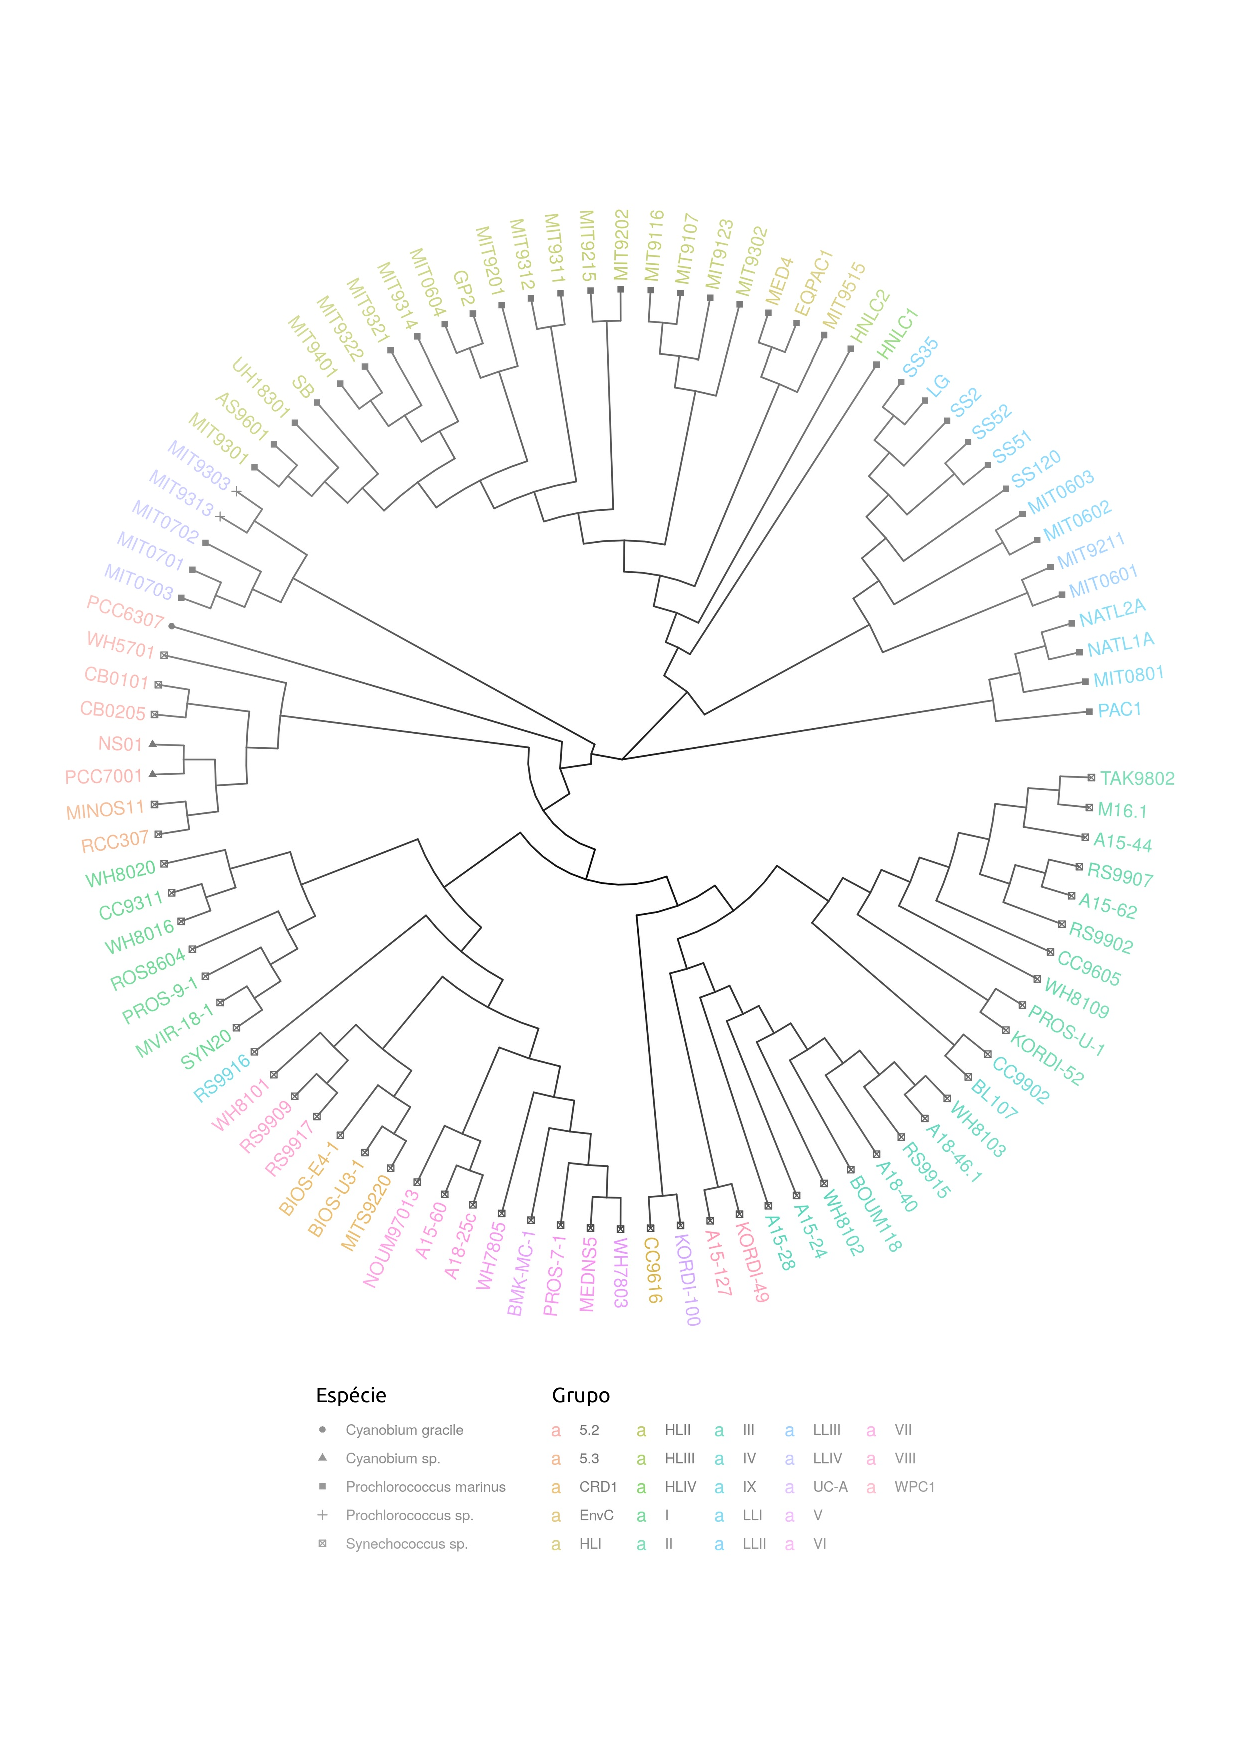
\includegraphics[width=.95\textwidth]{figures/REHDYXMS}
    \caption{Árvore filogenética baseada em rearranjos de genomas usando o Algoritmo~\ref{algorithm:MRFVALSC} com a estratégia gulosa e 97 genomas do sistema Cyanorak 2.1.} 
    \label{figure:REHDYXMS}
\end{figure}

Pela Figura~\ref{figure:REHDYXMS} (criada usando o pacote \texttt{treeio} da linguagem R~\cite{wang2020treeio}), observamos que a abordagem separa os organismos considerando as espécies e realizou bons agrupamentos. Vale ressaltar que a árvore foi baseada exclusivamente em informações de eventos de rearranjo.

% ------------------------------------------------------------------ %
\section{Abordagem Ponderada}
% ------------------------------------------------------------------ %

Nesta seção, apresentaremos os resultados considerando diferentes funções de custo para as variações com e sem sinais dos problemas \SbWIRI{}, \SbWIRT{} e \SbWIRTI{}.

A primeira função de custo, que chamamos de $W_1$, considera que os eventos de reversão e transposição possuem um custo de 1, enquanto um indel tem um custo equivalente a quantidade de nucleotídeos inseridos ou removidos da região intergênica. A seguir, descrevemos formalmente a função de custo $W_1$.

$$
  W_1(\beta) = \begin{cases}
      |x|, \textit{para } \beta = \delta_{(x)}^{(i)} \\
      1, \textit{para } \beta = \rho_{(x,y)}^{(i,j)} \\
      1, \textit{para } \beta = \tau_{(x,y,z)}^{(i,j,k)} \\
  \end{cases}
$$

Dada uma instância intergênica rígida com ou sem sinais $\mathcal{I}=((\pi,\breve\pi),(\iota,\breve\iota))$, denotamos por $IR(\mathcal{I}) = |\sum_{\breve\pi_i \in \breve\pi} \breve\pi_i - \sum_{\breve\iota_i \in \breve\iota} \breve\iota_i|$ a quantidade de nucleotídeos que precisam ser removidos ou inseridos no genoma de origem para que $\mathcal{I}$ seja uma instância balanceada. Note que reversões e transposições podem transferir nucleotídeos entre regiões intergênicas, mas não removem ou inserem nucleotídeos. Logo, em toda instância intergênica rígida com ou sem sinais $\mathcal{I}=((\pi,\breve\pi),(\iota,\breve\iota))$ para os problemas \SbWIRI{} e \SbWIRTI{} induz um custo mínimo de $IR(\mathcal{I})$, que nos dá os seguintes limites inferiores.

\begin{theorem}\label{theorem:IQACALLP}
Dada uma instância intergênica rígida sem sinais $\mathcal{I}=((\pi,\breve\pi),(\iota,\breve\iota))$ e com base na função de custo $W_1$, temos que:

\begin{tabular}{lll}
  $dw_{\SbWIRI}(\mathcal{I})$      & $ \ge $ & $\max(IR(\mathcal{I}),\frac{ib_1(\mathcal{I})}{2})$, \\ 
  $dw_{\SbWIRTI}(\mathcal{I})$     & $ \ge $ & $\max(IR(\mathcal{I}),\frac{ib_1(\mathcal{I})}{3})$.
\end{tabular}
\begin{proof}
Diretamente pelo Teorema~\ref{theorem:MPFPKHQO} e o custo mínimo de $IR(\mathcal{I})$ discutido anteriormente.
\end{proof}
\end{theorem}

\begin{theorem}\label{theorem:BOZETXBS}
Dada uma instância intergênica rígida com sinais $\mathcal{I}=((\pi,\breve\pi),(\iota,\breve\iota))$ e com base na função de custo $W_1$, temos que:

\begin{tabular}{lll}
  $dw_{\SbWIRI}(\mathcal{I})$      & $ \ge $ & $\max(IR(\mathcal{I}),\frac{ib_2(\mathcal{I})}{2})$, \\ 
  $dw_{\SbWIRTI}(\mathcal{I})$     & $ \ge $ & $\max(IR(\mathcal{I}),\frac{ib_2(\mathcal{I})}{3})$.
\end{tabular}
\begin{proof}
Diretamente pelo Teorema~\ref{theorem:NFVKZGKW} e o custo mínimo de $IR(\mathcal{I})$ discutido anteriormente.
\end{proof}
\end{theorem}

A seguir mostramos que, com base na função de custo $W_1$, é possível garantir aproximações para os problemas \SbWIRI{} e \SbWIRTI{} a partir de alguns dos algoritmos apresentados para o cenário não ponderado.

\begin{theorem}\label{theorem:BNWIOUVG}
Dada uma instância intergênica rígida sem sinais $\mathcal{I}=((\pi,\breve\pi),(\iota,\breve\iota))$, o Algoritmo~\ref{algorithm:LHOPSFVN}, com base na função de custo $W_1$, é uma $5$-aproximação para o problema \SbWIRI{}.
\end{theorem}
\begin{proof}
Note que o Algoritmo~\ref{algorithm:LHOPSFVN} transforma $(\pi,\breve\pi)$ em $(\iota,\breve\iota)$ utilizando no máximo $2ib_1(\mathcal{I})$ eventos de reversão e indel (Lema~\ref{lemma:XUDIVWPC}). Entretanto, caso $\mathcal{I}$ seja uma instância desbalanceada, então Algoritmo~\ref{algorithm:LHOPSFVN} aplica no máximo um indel com custo $IR(\mathcal{I})$. Caso contrário, apenas reversões são utilizadas. Logo, no pior caso, uma sequência de eventos de rearranjo fornecida pelo Algoritmo~\ref{algorithm:LHOPSFVN} tem um custo total de $IR(\mathcal{I}) + 2ib_1(\mathcal{I})$. Agora consideramos duas possibilidades:
\begin{itemize}
  \item $IR(\mathcal{I}) \ge \frac{ib_1(\mathcal{I})}{2}$: Neste caso, $2IR(\mathcal{I}) \ge ib_1(\mathcal{I})$ e o custo máximo da sequência de eventos de rearranjo fornecida pelo Algoritmo~\ref{algorithm:LHOPSFVN} é $5IR(\mathcal{I})$.
  \item $IR(\mathcal{I}) < \frac{ib_1(\mathcal{I})}{2}$: Neste caso, o custo máximo da sequência de eventos de rearranjo fornecida pelo Algoritmo~\ref{algorithm:LHOPSFVN} é $\frac{5ib_1(\mathcal{I})}{2}$.
\end{itemize}
Em ambos os casos, o custo máximo da sequência de eventos de rearranjo fornecida pelo Algoritmo~\ref{algorithm:LHOPSFVN} dividido pelo valor do limitante inferior, apresentado no Teorema~\ref{theorem:IQACALLP}, é igual a cinco e o teorema segue.
\end{proof}

\begin{theorem}\label{theorem:JKFXFCMF}
Dada uma instância intergênica rígida com sinais $\mathcal{I}=((\pi,\breve\pi),(\iota,\breve\iota))$, o Algoritmo~\ref{algorithm:QKCVERGO}, com base na função de custo $W_1$, é uma $5$-aproximação para o problema \SbWIRI{}.
\end{theorem}
\begin{proof}
A prova é similar a descrita no Teorema~\ref{theorem:BNWIOUVG}, mas considerando o Algoritmo~\ref{algorithm:QKCVERGO}, que utiliza o Algoritmo~\ref{algorithm:LHOPSFVN} em parte de sua execução, e o limitante inferior apresentado no Teorema~\ref{theorem:BOZETXBS}.
\end{proof}

\begin{theorem}\label{theorem:YATYVCZX}
Dada uma instância intergênica rígida sem sinais $\mathcal{I}=((\pi,\breve\pi),(\iota,\breve\iota))$, o Algoritmo~\ref{algorithm:YIZYUGZZ}, com base na função de custo $W_1$, é uma $5$-aproximação para o problema \SbWIRTI{}.
\end{theorem}
\begin{proof}
Pelo Lema~\ref{lemma:MUTXDAUG}, o Algoritmo~\ref{algorithm:YIZYUGZZ} utiliza no máximo $\frac{4ib_1(\mathcal{I})}{3}$ e $\frac{4ib_1(\mathcal{I})}{3} + 1$ eventos de reversão, transposição e indel para transformar $(\pi,\breve\pi)$ em $(\iota,\breve\iota)$ se $\mathcal{I}$ for balanceada e desbalanceada, respectivamente. Entretanto, caso $\mathcal{I}$ seja uma instância desbalanceada, então Algoritmo~\ref{algorithm:YIZYUGZZ} aplica no máximo um indel com custo $IR(\mathcal{I})$. Caso contrário, apenas reversões e transposições são utilizadas. Logo, no pior caso, uma sequência de eventos de rearranjo fornecida pelo Algoritmo~\ref{algorithm:YIZYUGZZ} tem um custo total de $IR(\mathcal{I}) + \frac{4ib_1(\mathcal{I})}{3}$. Agora consideramos duas possibilidades:
\begin{itemize}
  \item $IR(\mathcal{I}) \ge \frac{ib_1(\mathcal{I})}{3}$: Neste caso, $3IR(\mathcal{I}) \ge ib_1(\mathcal{I})$ e o custo máximo da sequência de eventos de rearranjo fornecida pelo Algoritmo~\ref{algorithm:YIZYUGZZ} é $IR(\mathcal{I}) + \frac{12IR(\mathcal{I})}{3} = 5IR(\mathcal{I})$.
  \item $IR(\mathcal{I}) < \frac{ib_1(\mathcal{I})}{3}$: Neste caso, o custo máximo da sequência de eventos de rearranjo fornecida pelo Algoritmo~\ref{algorithm:YIZYUGZZ} é $\frac{ib_1(\mathcal{I})}{3} + \frac{4ib_1(\mathcal{I})}{3} = \frac{5ib_1(\mathcal{I})}{3}$.
\end{itemize}
Em ambos os casos, o custo máximo da sequência de eventos de rearranjo fornecida pelo Algoritmo~\ref{algorithm:YIZYUGZZ} dividido pelo valor do limitante inferior, apresentado no Teorema~\ref{theorem:IQACALLP}, é igual a cinco e o teorema segue.
\end{proof}

\begin{theorem}\label{theorem:XMRIBCHD}
Dada uma instância intergênica rígida com sinais $\mathcal{I}=((\pi,\breve\pi),(\iota,\breve\iota))$, o Algoritmo~\ref{algorithm:EQALRDVE}, com base na função de custo $W_1$, é uma $5$-aproximação para o problema \SbWIRI{}.
\end{theorem}
\begin{proof}
A prova é similar a descrita no Teorema~\ref{theorem:YATYVCZX}, mas considerando o Algoritmo~\ref{algorithm:EQALRDVE}, que utiliza o Algoritmo~\ref{algorithm:YIZYUGZZ} em parte de sua execução, e o limitante inferior apresentado no Teorema~\ref{theorem:BOZETXBS}.
\end{proof}

A segunda função de custo, chamada de $W_2$, é baseada no fato de que um indel afeta apenas uma região intergênica. Dessa forma, consideramos que o evento de indel possui a metade do custo de um evento de reversão ou transposição. A seguir, descrevemos formalmente a função de custo $W_2$.

$$
  W_2(\beta) = \begin{cases}
      \frac{1}{2}, \textit{para } \beta = \delta_{(x)}^{(i)} \\
      1, \textit{para } \beta = \rho_{(x,y)}^{(i,j)} \\
      1, \textit{para } \beta = \tau_{(x,y,z)}^{(i,j,k)} \\
  \end{cases}
$$

Com base nos custos da função $W_2$, obtemos para as variações com e sem sinais do problema \SbWIRTI{} os seguintes limitantes inferiores.

\begin{theorem}\label{theorem:HFHHZDMV}
Dada uma instância intergênica rígida sem sinais $\mathcal{I}=((\pi,\breve\pi),(\iota,\breve\iota))$ e com base na função de custo $W_2$, temos que $dw_{\SbWIRTI}(\mathcal{I}) \ge \frac{ib_1(\mathcal{I})}{3}$.
\begin{proof}
Pelos lemas~\ref{lemma:KFFPUBQG}, \ref{lemma:IUJZCMMV} e \ref{lemma:KWIVENLG}, sabemos que os eventos de reversão, transposição e indel removem por operação, no máximo, $2$, $3$ e $1$ breakpoint tipo um, respectivamente. Com base no melhor caso de cada evento de rearranjo e na função de custo $W_2$, temos que:
$$dw_{\SbWIRTI}(\mathcal{I}) \ge \min\left(\frac{ib_1(\mathcal{I})}{2} \times 1,\frac{ib_1(\mathcal{I})}{3} \times 1, ib_1(\mathcal{I}) \times \frac{1}{2}\right) = \frac{ib_1(\mathcal{I})}{3},$$ e o teorema segue.
\end{proof}
\end{theorem}

\begin{theorem}\label{theorem:IXYMBAWM}
Dada uma instância intergênica rígida com sinais $\mathcal{I}=((\pi,\breve\pi),(\iota,\breve\iota))$ e com base na função de custo $W_2$, temos que $dw_{\SbWIRTI}(\mathcal{I}) \ge \frac{ib_2(\mathcal{I})}{3}$.
\begin{proof}
A prova é similar a descrita no Teorema~\ref{theorem:HFHHZDMV}, mas considerando os lemas~\ref{lemma:IKBNJWMY}, \ref{lemma:MYVALTSG} e \ref{lemma:KXIYYHHL}.
\end{proof}
\end{theorem}

\begin{lemma}\label{lemma:XLFWKWTV}
Dada uma instância intergênica rígida sem sinais $\mathcal{I}=((\pi,\breve\pi),(\iota,\breve\iota))$ e sejam $(\pi_i,\pi_{i+1})$ e $(\pi_j,\pi_{j+1})$ breakpoints conectados, então é possível remover pelo menos um breakpoint tipo um de $\mathcal{I}$ utilizando no máximo uma reversão, uma transposição ou dois indels.
\end{lemma}
\begin{proof}
Sem perda de generalidade assuma que $i < j$, como os breakpoints $(\pi_i,\pi_{i+1})$ e $(\pi_j,\pi_{j+1})$ estão conectados, por definição, uma das seguintes possibilidades deve ocorrer:
\begin{enumerate}[i.]
  \item O par de elementos $(\pi_i,\pi_{j})$ ou $(\pi_{i+1},\pi_{j+1})$ não formam uma adjacência intergênica, são consecutivos em $\iota$ e $\breve\pi_{i+1} + \breve\pi_{j+1} \ge \breve\iota_k$, onde $\breve\iota_k$ é o tamanho da região intergênica entre o par de elementos consecutivos em $\iota$. Aplique uma reversão como descrito no caso $i$ do Lema~\ref{lemma:IMYFBWDY}.
  \item O par  de elementos $(\pi_i,\pi_{j+1})$ não formam uma adjacência intergênica, são consecutivos em $\iota$ e $\breve\pi_{i+1} + \breve\pi_{j+1} \ge \breve\iota_k$, onde $\breve\iota_k$ é o tamanho da região intergênica entre o par de elementos consecutivos em $\iota$. Aplique uma transposição como descrito no caso $ii$ do Lema~\ref{lemma:SIAFJFDO}.
  \item O par de elementos $(\pi_{i+1},\pi_{j})$ não formam uma adjacência intergênica, são consecutivos em $\iota$ e $\breve\pi_{i+1} + \breve\pi_{j+1} \ge \breve\iota_k$, onde $\breve\iota_k$ é o tamanho da região intergênica entre o par de elementos consecutivos em $\iota$. Aplique uma transposição como descrito no caso $iii$ do Lema~\ref{lemma:SIAFJFDO}.
  \item O par de elementos $(\pi_{i},\pi_{i+1})$ ou $(\pi_{j},\pi_{j+1})$ não formam uma adjacência intergênica, são consecutivos em $\iota$ e $\breve\pi_{i+1} + \breve\pi_{j+1} \ge \breve\iota_k$, onde $\breve\iota_k$ é o tamanho da região intergênica entre o par de elementos consecutivos em $\iota$. Neste caso, $(\pi_{i},\pi_{i+1})$ ou $(\pi_{j},\pi_{j+1})$ deve ser um breakpoint forte. Caso $(\pi_{i},\pi_{i+1})$ seja um breakpoint forte, então ele pode ser subcarregado ou sobrecarregado. Caso $(\pi_{i},\pi_{i+1})$ seja subcarregado, então aplique a sequência de dois indels $(\delta^{i+1}_{(x)}, \delta^{j+1}_{(-x)})$, com $x=|\breve\pi_{i+1} - \breve\iota_{\max(\pi_i, \pi_{i+1})}|$. Caso contrário, aplique a sequência de dois indels $(\delta^{i+1}_{(-x)}, \delta^{j+1}_{(x)})$, com $x=|\breve\pi_{i+1} - \breve\iota_{\max(\pi_i, \pi_{i+1})}|$. Caso $(\pi_{j},\pi_{j+1})$ seja um breakpoint forte, basta replicar a sequência de indels considerando a mudança no breakpoint. Note que essa senquência sempre pode ser aplicada, pois os dois breakpoints estão conectados. Além disso, o breakpoint tipo um $(\pi_i,\pi_{i+1})$ é removido sem afetar quantidade de total de nucleotídeos de $\mathcal{I}$.  
\end{enumerate}
Note que o caso $(i)$ aplica apenas um reversão e remove pelo menos um breakpoint tipo um. Os casos $(ii)$ e $(iii)$ aplicam apenas uma transposição e removem pelo menos um breakpoint tipo um. Por fim, o caso $(iv)$ remove pelo menos um breakpoint tipo um após aplicar dois indels. Logo, o lema segue.
\end{proof}

A seguir apresentamos para a variação sem sinais do problema \SbWIRTI{} o Algoritmo~\ref{algorithm:DYNWURLY}.

\begin{algorithm}[!tbh]
  \caption{Um algoritmo de aproximação para o problema \SbWIRTI{}.\label{algorithm:DYNWURLY}}
  \Entrada{Uma instância intergênica rígida sem sinais $\mathcal{I}=((\pi,\breve\pi),(\iota,\breve\iota))$}
  \Saida{Uma sequência de reversões transposições e indels $S$, tal que $(\pi,\breve\pi) \cdot S = (\iota,\breve\iota)$}
    Seja $S \gets ()$ \\
    \tcp{Lema~\ref{lemma:QGOIQLZD}}
    \Se{$\sum_{i=1}^{n+1}\breve\pi_i < \sum_{i=1}^{n+1}\breve\iota_i$}{
      $S' \gets (\delta_1)$ \\
      $S \gets S + S'$ \\
      $\mathcal{I} \gets ((\pi, \breve\pi) \cdot S',(\iota,\breve\iota))$ \\
    }
    \Enqto{$ib_1(\mathcal{I}) > 1$}{
      \tcp{Lema~\ref{lemma:WYEZMYTM}}
      $(\pi_i,\pi_{i+1})$, $(\pi_j,\pi_{j+1}) \gets $ encontre um par de breakpoints conectados \\
      \tcp{Lema~\ref{lemma:XLFWKWTV}}
      \Se{$(\pi_i,\pi_{i+1})$, $(\pi_j,\pi_{j+1})$ pertence ao caso $i$}{
        $S' \gets (\rho_1)$ \\
      }\SenaoSe{$(\pi_i,\pi_{i+1})$, $(\pi_j,\pi_{j+1})$ pertence ao caso $ii$}{
        $S' \gets (\tau_1)$ \\
      }\SenaoSe{$(\pi_i,\pi_{i+1})$, $(\pi_j,\pi_{j+1})$ pertence ao caso $iii$}{
        $S' \gets (\tau_1)$ \\
      }\SenaoSe{$(\pi_i,\pi_{i+1})$, $(\pi_j,\pi_{j+1})$ pertence ao caso $iv$}{
        $S' \gets (\delta_1,\delta_2)$ \\
      }
      $S \gets S + S'$ \\
      $\mathcal{I} \gets ((\pi, \breve\pi) \cdot S',(\iota,\breve\iota))$ \\
    }
    \tcp{Lema~\ref{lemma:QNHGBLYF}}
    \Se{$ib(\mathcal{I}) = 1$}{
      $S' \gets (\delta_1)$ \\
      $S \gets S + S'$ \\
      $\mathcal{I} \gets ((\pi, \breve\pi) \cdot S',(\iota,\breve\iota))$ \\
    }
  \Retorna{S}
\end{algorithm}

\begin{lemma}\label{lemma:IKTEYDRR}
Dada uma instância intergênica rígida sem sinais $\mathcal{I}=((\pi,\breve\pi),(\iota,\breve\iota))$, o Algoritmo~\ref{algorithm:DYNWURLY}, com base na função de custo $W_2$, transforma $(\pi,\breve\pi)$ em $(\iota,\breve\iota)$ utilizando uma sequência de eventos de reversão, transposição e indel $S$, com um custo total de no máximo $ib_1(\mathcal{I})$.
\end{lemma}
\begin{proof}
  Podemos analisar o Algoritmo~\ref{algorithm:DYNWURLY} considerando três cenários:
  \begin{itemize}
    \item $\sum_{i=1}^{n+1}\breve\pi_i < \sum_{i=1}^{n+1}\breve\iota_i$, neste cenários o Algoritmo~\ref{algorithm:DYNWURLY} aplica um indel (linhas 2-5) que pode não remover nenhum breakpoint tipo um, mas torna $\mathcal{I}$ em uma instância balanceada. Caso ainda existam breakpoints em $\mathcal{I}$, então o laço de repetição (linhas 6-17) remove, por iteração, pelo menos um breakpoint tipo um utilizando no máximo uma reversão, uma transposição ou dois indels (Lema~\ref{lemma:XLFWKWTV}). Esse processo repete-se até que todos os breakpoints tipo um de $\mathcal{I}$ sejam removidos. Como todos os breakpoints tipo um são removidos, então $(\pi,\breve\pi)$ é transformada em $(\iota,\breve\iota)$. Note que se o indel aplicado inicialmente não remover nenhum breakpoint tipo um, então pelo menos uma reversão, uma transposição ou dois indels são aplicados em seguida. Além disso, pelo Lema~\ref{lemma:WSPRPLAH}, podemos deduzir que caso a última operação que transforma $(\pi,\breve\pi)$ em $(\iota,\breve\iota)$ seja uma reversão ou uma transposição, então ela deve obrigatoriamente remover pelo menos dois breakpoints tipo um. Caso essa operação seja um indel, então as duas últimas operações são indels e ambas removem um breakpoint tipo um. Isso implica que o custo total da sequência fornecida pelo Algoritmo~\ref{algorithm:DYNWURLY} é de no máximo $ib_1(\mathcal{I})$.
    \item $\sum_{i=1}^{n+1}\breve\pi_i = \sum_{i=1}^{n+1}\breve\iota_i$, para esse cenários o Algoritmo~\ref{algorithm:DYNWURLY} executará o laço de repetição (linhas 6-17) que remove, por iteração, pelo menos um breakpoint tipo um utilizando no máximo uma reversão, uma transposição ou dois indels (Lema~\ref{lemma:XLFWKWTV}). Implicando também que o custo total da sequência fornecida pelo Algoritmo~\ref{algorithm:DYNWURLY} é de no máximo $ib_1(\mathcal{I})$.
    \item $\sum_{i=1}^{n+1}\breve\pi_i > \sum_{i=1}^{n+1}\breve\iota_i$, neste último cenário enquanto $ib_1(\mathcal{I})$ for maior que um, o Algoritmo~\ref{algorithm:DYNWURLY} aplica no máximo uma reversão, uma transposição ou dois indels em cada iteração do laço de repetição (linhas 6-17) que removem pelo menos um breakpoint tipo um. Por fim, um indel é aplicado (linhas 19-22) transformando $(\pi,\breve\pi)$ em $(\iota,\breve\iota)$. O custo para remover cada breakpoint nesse caso é de no máximo um. Logo, o custo total da sequência fornecida pelo Algoritmo~\ref{algorithm:DYNWURLY} é de no máximo $ib_1(\mathcal{I})$. 
  \end{itemize}
  Nos três cenários o Algoritmo~\ref{algorithm:DYNWURLY} transforma $(\pi,\breve\pi)$ em $(\iota,\breve\iota)$ utilizando uma sequência de reversões, transposições e indels com um custo total de no máximo $ib_1(\mathcal{I})$, e o lema segue.
\end{proof}

Note que o tempo de execução do Algoritmo~\ref{algorithm:DYNWURLY} é $\mathcal{O(n^2)}$, uma vez que para encontrar um par conectado de breakpoints requer um tempo linear e esse processo pode repetir-se por até $ib_1(\mathcal{I}) \le n + 1$ vezes.

\begin{theorem}\label{theorem:HXFXWAIA}
Dada uma instância intergênica rígida sem sinais $\mathcal{I}=((\pi,\breve\pi),(\iota,\breve\iota))$, o Algoritmo~\ref{algorithm:DYNWURLY}, com base na função de custo $W_2$, é uma $3$-aproximação para o problema \SbWIRTI{}.
\end{theorem}
\begin{proof}
Pelo Lema~\ref{lemma:IKTEYDRR}, o Algoritmo~\ref{algorithm:DYNWURLY} transforma $(\pi,\breve\pi)$ em $(\iota,\breve\iota)$ utilizando uma sequência de eventos de reversão, transposição e indel $S$, com um custo total de no máximo $ib_1(\mathcal{I})$. Pelo limitante inferior, apresentado no Teorema~\ref{theorem:HFHHZDMV}, temos que $dw_{\SbWIRTI}(\mathcal{I}) \ge \frac{ib_1(\mathcal{I})}{3}$. Logo, o teorema segue.
\end{proof}

A seguir apresentamos para a variação com sinais do problema \SbWIRTI{} o Algoritmo~\ref{algorithm:HHROEWVE}.

\begin{algorithm}[!tbh]
  \caption{Um algoritmo de aproximação para o problema \SbWIRTI{}.\label{algorithm:HHROEWVE}}
  \Entrada{Uma instância intergênica rígida com sinais $\mathcal{I}=((\pi,\breve\pi),(\iota,\breve\iota))$}
  \Saida{Uma sequência de eventos de reversão, transposição e indel $S$, tal que $(\pi,\breve\pi) \cdot S = (\iota,\breve\iota)$}
  \tcp{Lema~\ref{lemma:FKOCCOYY}}
  $\mathcal{I'} \gets \mathcal{F}(\mathcal{I})$ \\
  Seja $S'$ uma sequência de eventos de reversão, transposição e indel fornecida pelo Algoritmo~\ref{algorithm:DYNWURLY} para a instância $\mathcal{I'}$ \\
  \tcp{Lema~\ref{lemma:GTTULLOM}}
  $S\gets \mathcal{G}(S')$ \\
  \Retorna{S}
\end{algorithm}

\begin{lemma}\label{lemma:MBYKFLMR}
Dada uma instância intergênica rígida com sinais $\mathcal{I}=((\pi,\breve\pi),(\iota,\breve\iota))$, o Algoritmo~\ref{algorithm:DYNWURLY}, com base na função de custo $W_2$, transforma $(\pi,\breve\pi)$ em $(\iota,\breve\iota)$ utilizando uma sequência de eventos de reversão, transposição e indel $S$, com um custo total de no máximo $ib_2(\mathcal{I})$.
\end{lemma}
\begin{proof}
Note que o Algoritmo~\ref{algorithm:DYNWURLY} fornece um sequência de reversões, tranposições e indels que afetam apenas breakpoints tipo um. Logo, nunhuma adjacência intergênica de $\mathcal{I'}$ é afetada. Além disso, pelo Lema~\ref{lemma:IKTEYDRR}, o Algoritmo~\ref{algorithm:DYNWURLY} utiliza uma sequência de eventos de reversão, transposição e indel, com um custo total de no máximo $ib_1(\mathcal{I'})$. Pelo Lema~\ref{lemma:GTTULLOM}, temos que $(\pi,\breve\pi) \cdot S = (\iota,\breve\iota)$ e $|S| = |S'|$. Além disso, $S$ e $|S'|$ possuem a mesma quantidade de operações por tipo. Pelo Lema~\ref{lemma:FKOCCOYY}, temos que $ib_1(\mathcal{I'}) = ib_2(\mathcal{I})$. Logo, o custo total da sequência de eventos de reversão, transposição e indel fornecida pelo Algoritmo~\ref{algorithm:HHROEWVE} é de no máximo $ib_2(\mathcal{I})$.
\end{proof}

O Algoritmo~\ref{algorithm:HHROEWVE} também possui um tempo de execução de $\mathcal{O}(n^2)$, uma vez que as funções $\mathcal{F}$ e $\mathcal{G}$ executam em tempo linear e o Algoritmo~\ref{algorithm:DYNWURLY}, no pior caso, requer um tempo quadrático.

\begin{theorem}\label{theorem:MJXOZGOO}
Dada uma instância intergênica rígida com sinais $\mathcal{I}=((\pi,\breve\pi),(\iota,\breve\iota))$, o Algoritmo~\ref{algorithm:HHROEWVE}, com base na função de custo $W_2$, é uma $3$-aproximação para o problema \SbWIRTI{}.
\end{theorem}
\begin{proof}
Pelo Lema~\ref{lemma:MBYKFLMR}, o Algoritmo~\ref{algorithm:HHROEWVE} transforma $(\pi,\breve\pi)$ em $(\iota,\breve\iota)$ utilizando uma sequência de eventos de reversão, transposição e indel, com um custo total de no máximo $ib_2(\mathcal{I})$. Pelo limitante inferior, apresentado no Teorema~\ref{theorem:IXYMBAWM}, temos que $dw_{\SbWIRTI}(\mathcal{I}) \ge \frac{ib_2(\mathcal{I})}{3}$. Logo, o teorema segue.
\end{proof}

A terceira função de custo, chamada de $W_3$, é baseada na proporção de regiões intergêncas afetadas por cada evento de rearranjo~\cite{2018-alexandrino-etal}. A seguir, descrevemos formalmente a função de custo $W_3$.

$$
  W_3(\beta) = \begin{cases}
      \frac{1}{2}, \textit{para } \beta = \delta_{(x)}^{(i)} \\
      1, \textit{para } \beta = \rho_{(x,y)}^{(i,j)} \\
      \frac{3}{2}, \textit{para } \beta = \tau_{(x,y,z)}^{(i,j,k)} \\
  \end{cases}
$$

Com base nos custos da função $W_3$, obtemos para as variações com e sem sinais do problema \SbWIRTI{} os seguintes limitantes inferiores.

\begin{theorem}\label{theorem:BFKDUKUF}
Dada uma instância intergênica rígida sem sinais $\mathcal{I}=((\pi,\breve\pi),(\iota,\breve\iota))$ e com base na função de custo $W_3$, temos que $dw_{\SbWIRTI}(\mathcal{I}) \ge \frac{ib_1(\mathcal{I})}{2}$.
\begin{proof}
Pelos lemas~\ref{lemma:KFFPUBQG}, \ref{lemma:IUJZCMMV} e \ref{lemma:KWIVENLG}, sabemos que os eventos de reversão, transposição e indel removem por operação, no máximo, $2$, $3$ e $1$ breakpoint tipo um, respectivamente. Com base no melhor caso de cada evento de rearranjo e na função de custo $W_3$, temos que:
$$dw_{\SbWIRTI}(\mathcal{I}) \ge \min\left(\frac{ib_1(\mathcal{I})}{2} \times 1,\frac{ib_1(\mathcal{I})}{3} \times \frac{3}{2}, ib_1(\mathcal{I}) \times \frac{1}{2}\right) = \frac{ib_1(\mathcal{I})}{2},$$ e o teorema segue.
\end{proof}
\end{theorem}

\begin{theorem}\label{theorem:ACJPZCWD}
Dada uma instância intergênica rígida com sinais $\mathcal{I}=((\pi,\breve\pi),(\iota,\breve\iota))$ e com base na função de custo $W_2$, temos que $dw_{\SbWIRTI}(\mathcal{I}) \ge \frac{ib_2(\mathcal{I})}{2}$.
\begin{proof}
A prova é similar a descrita no Teorema~\ref{theorem:BFKDUKUF}, mas considerando os lemas~\ref{lemma:IKBNJWMY}, \ref{lemma:MYVALTSG} e \ref{lemma:KXIYYHHL}.
\end{proof}
\end{theorem}

\begin{lemma}\label{lemma:FESYSSFB}
Dada uma instância intergênica rígida sem sinais $\mathcal{I}=((\pi,\breve\pi),(\iota,\breve\iota))$, o Algoritmo~\ref{algorithm:DYNWURLY}, com base na função de custo $W_3$, transforma $(\pi,\breve\pi)$ em $(\iota,\breve\iota)$ utilizando uma sequência de eventos de reversão, transposição e indel $S$, com um custo total de no máximo $\frac{3ib_1(\mathcal{I})}{2}$.
\end{lemma}
\begin{proof}
  A prova é similar a descrita no Lema~\ref{lemma:IKTEYDRR} considerando a função de custo $W_3$.
\end{proof}

\begin{theorem}\label{theorem:YFYDIUAB}
Dada uma instância intergênica rígida sem sinais $\mathcal{I}=((\pi,\breve\pi),(\iota,\breve\iota))$, o Algoritmo~\ref{algorithm:DYNWURLY}, com base na função de custo $W_3$, é uma $3$-aproximação para o problema \SbWIRTI{}.
\end{theorem}
\begin{proof}
Pelo Lema~\ref{lemma:FESYSSFB}, o Algoritmo~\ref{algorithm:DYNWURLY} transforma $(\pi,\breve\pi)$ em $(\iota,\breve\iota)$ utilizando uma sequência de eventos de reversão, transposição e indel $S$, com um custo total de no máximo $\frac{3ib_1(\mathcal{I})}{2}$. Pelo limitante inferior, apresentado no Teorema~\ref{theorem:BFKDUKUF}, temos que $dw_{\SbWIRTI}(\mathcal{I}) \ge \frac{ib_1(\mathcal{I})}{2}$. Logo, o teorema segue.
\end{proof}

\begin{lemma}\label{lemma:HRFGEWNU}
Dada uma instância intergênica rígida com sinais $\mathcal{I}=((\pi,\breve\pi),(\iota,\breve\iota))$, o Algoritmo~\ref{algorithm:HHROEWVE}, com base na função de custo $W_3$, transforma $(\pi,\breve\pi)$ em $(\iota,\breve\iota)$ utilizando uma sequência de eventos de reversão, transposição e indel $S$, com um custo total de no máximo $\frac{3ib_2(\mathcal{I})}{2}$.
\end{lemma}
\begin{proof}
  A prova é similar a descrita no Lema~\ref{lemma:MBYKFLMR} considerando a função de custo $W_3$.
\end{proof}

\begin{theorem}\label{theorem:UMSMTVTN}
Dada uma instância intergênica rígida com sinais $\mathcal{I}=((\pi,\breve\pi),(\iota,\breve\iota))$, o Algoritmo~\ref{algorithm:HHROEWVE}, com base na função de custo $W_3$, é uma $3$-aproximação para o problema \SbWIRTI{}.
\end{theorem}
\begin{proof}
Pelo Lema~\ref{lemma:HRFGEWNU}, o Algoritmo~\ref{algorithm:HHROEWVE} transforma $(\pi,\breve\pi)$ em $(\iota,\breve\iota)$ utilizando uma sequência de eventos de reversão, transposição e indel $S$, com um custo total de no máximo $\frac{3ib_2(\mathcal{I})}{2}$. Pelo limitante inferior, apresentado no Teorema~\ref{theorem:ACJPZCWD}, temos que $dw_{\SbWIRTI}(\mathcal{I}) \ge \frac{ib_2(\mathcal{I})}{2}$. Logo, o teorema segue.
\end{proof}

A seguir apresentamos duas funções de custo para o problema \SbWIRT{} que são bem aceitas na literatura em modelos compostos pelos eventos conservativos de reversão e transposição. A primeira função de custo, chamada de $W_4$, adota o custo $1$ e $2$ para os eventos de reversão e transposição, respectivamente~\cite{2002-eriksen}. A segunda função de custo, chamada de $W_5$, adota os custos $1$ e $\frac{3}{2}$ para os eventos de reversão e transposição, respectivamente~\cite{2019a-oliveira-etal}. A seguir, descrevemos formalmente as funções de custo $W_4$ e $W_5$.

$$
  W_4(\beta) = \begin{cases}
      1, \textit{para } \beta = \rho_{(x,y)}^{(i,j)} \\
      2, \textit{para } \beta = \tau_{(x,y,z)}^{(i,j,k)} \\
  \end{cases}
$$ 

$$
  W_5(\beta) = \begin{cases}
      1, \textit{para } \beta = \rho_{(x,y)}^{(i,j)} \\
      \frac{3}{2}, \textit{para } \beta = \tau_{(x,y,z)}^{(i,j,k)} \\
  \end{cases}
$$

Com base nos custos das funções $W_4$ e $W_5$, obtemos para as variações com e sem sinais do problema \SbWIRT{} os seguintes limitantes inferiores.

\begin{theorem}\label{theorem:TUSWAWTT}
Dada uma instância intergênica rígida balanceada sem sinais $\mathcal{I}=((\pi,\breve\pi),(\iota,\breve\iota))$ e com base na função de custo $W_4$, temos que $dw_{\SbWIRT}(\mathcal{I}) \ge \frac{ib_1(\mathcal{I})}{2}$.
\begin{proof}
Pelos lemas~\ref{lemma:KFFPUBQG}, \ref{lemma:IUJZCMMV} e \ref{lemma:KWIVENLG}, sabemos que os eventos de reversão, transposição e indel removem por operação, no máximo, $2$, $3$ e $1$ breakpoint tipo um, respectivamente. Com base no melhor caso de cada evento de rearranjo e na função de custo $W_4$, temos que:
$$dw_{\SbWIRTI}(\mathcal{I}) \ge \min\left(\frac{ib_1(\mathcal{I})}{2} \times 1,\frac{ib_1(\mathcal{I})}{3} \times 2\right) = \frac{ib_1(\mathcal{I})}{2},$$ e o teorema segue.
\end{proof}
\end{theorem}

\begin{theorem}\label{theorem:RPTOVHAP}
Dada uma instância intergênica rígida balanceada com sinais $\mathcal{I}=((\pi,\breve\pi),(\iota,\breve\iota))$ e com base na função de custo $W_4$, temos que $dw_{\SbWIRT}(\mathcal{I}) \ge \frac{ib_2(\mathcal{I})}{2}$.
\begin{proof}
A prova é similar a descrita no Teorema~\ref{theorem:TUSWAWTT}, mas considerando os lemas~\ref{lemma:IKBNJWMY}, \ref{lemma:MYVALTSG} e \ref{lemma:KXIYYHHL}.
\end{proof}
\end{theorem}

\begin{lemma}\label{lemma:DDSJVECJ}
Dada uma instância intergênica rígida balanceada sem sinais $\mathcal{I}=((\pi,\breve\pi),\break(\iota,\breve\iota))$, o Algoritmo~\ref{algorithm:JQHVZACM}, com base na função de custo $W_4$, transforma $(\pi,\breve\pi)$ em $(\iota,\breve\iota)$ utilizando uma sequência de eventos de reversão e transposição $S$, com um custo total de no máximo $2ib_1(\mathcal{I})$.
\end{lemma}
\begin{proof}
Pelo Lema~\ref{lemma:RNJHXOWZ}, sabemos que o Algoritmo~\ref{algorithm:JQHVZACM} transforma $(\pi,\breve\pi)$ em $(\iota,\breve\iota)$. Para obtermos o custo total máximo de uma sequência de reversões e transposições fornecida pelo Algoritmo~\ref{algorithm:JQHVZACM} vamos considerar suas duas fases: (i) remoção de breakpoints sobrecarregados, nessa fase cada breakpoint tipo um é removido com um custo médio de $2$, no pior caso; (ii) remoção de breakpoints suaves, no pior caso, cada breakpoint tipo um é removido por uma transposição, que tem custo $2$. Dessa forma, o custo total máximo de uma sequência de reversões e transposições fornecida pelo Algoritmo~\ref{algorithm:JQHVZACM} é $2ib_1(\mathcal{I})$, e o lema segue. 
\end{proof}

\begin{theorem}\label{theorem:CQXBDUDY}
Dada uma instância intergênica rígida balanceada sem sinais $\mathcal{I}=((\pi,\breve\pi),(\iota,\breve\iota))$, o Algoritmo~\ref{algorithm:JQHVZACM}, com base na função de custo $W_4$, é uma $4$-aproximação para o problema \SbWIRT{}.
\end{theorem}
\begin{proof}
Pelo Lema~\ref{lemma:DDSJVECJ}, o Algoritmo~\ref{algorithm:JQHVZACM}, com base na função de custo $W_4$, transforma $(\pi,\breve\pi)$ em $(\iota,\breve\iota)$ utilizando uma sequência de eventos de reversão e transposição com um custo total de no máximo $2ib_1(\mathcal{I})$. Pelo limitante inferior, apresentado no Teorema~\ref{theorem:TUSWAWTT}, temos que $dw_{\SbWIRT}(\mathcal{I}) \ge \frac{ib_2(\mathcal{I})}{2}$. Logo, o teorema segue.
\end{proof}

A seguir apresentamos para a variação com sinais do problema \SbWIRT{} o Algoritmo~\ref{algorithm:JRRYCBXN}.

\begin{algorithm}[!tbh]
  \caption{Um algoritmo de aproximação para o problema \SbWIRT{}.\label{algorithm:JRRYCBXN}}
  \Entrada{Uma instância intergênica rígida com sinais $\mathcal{I}=((\pi,\breve\pi),(\iota,\breve\iota))$}
  \Saida{Uma sequência de eventos de reversão e transposição $S$, tal que $(\pi,\breve\pi) \cdot S = (\iota,\breve\iota)$}
  \tcp{Lema~\ref{lemma:FKOCCOYY}}
  $\mathcal{I'} \gets \mathcal{F}(\mathcal{I})$ \\
  Seja $S'$ uma sequência de eventos de reversão e transposição fornecida pelo Algoritmo~\ref{algorithm:JQHVZACM} \\
  \tcp{Lema~\ref{lemma:GTTULLOM}}
  $S\gets \mathcal{G}(S')$ \\
  \Retorna{S}
\end{algorithm}

\begin{lemma}\label{lemma:TMZVZPOF}
Dada uma instância intergênica rígida balanceada com sinais $\mathcal{I}=((\pi,\breve\pi),\break(\iota,\breve\iota))$, o Algoritmo~\ref{algorithm:JRRYCBXN}, com base na função de custo $W_4$, transforma $(\pi,\breve\pi)$ em $(\iota,\breve\iota)$ utilizando uma sequência de eventos de reversão e transposição $S$, com um custo total de no máximo $2ib_2(\mathcal{I})$.
\end{lemma}
\begin{proof}
Note que o Algoritmo~\ref{algorithm:JQHVZACM} fornece um sequência de reversões e tranposições que afetam apenas breakpoints tipo um. Logo, nunhuma adjacência intergênica de $\mathcal{I'}$ é afetada. Além disso, pelo Lema~\ref{lemma:DDSJVECJ}, o Algoritmo~\ref{algorithm:JQHVZACM} utiliza uma sequência de eventos de reversão e transposição com um custo total de no máximo $ib_1(\mathcal{I'})$ para transformar $(\pi',\breve\pi')$ em $(\iota',\breve\iota')$. Pelo Lema~\ref{lemma:GTTULLOM}, temos que $(\pi,\breve\pi) \cdot S = (\iota,\breve\iota)$ e $|S| = |S'|$. Além disso, $S$ e $|S'|$ possuem a mesma quantidade de operações por tipo. Pelo Lema~\ref{lemma:FKOCCOYY}, temos que $ib_1(\mathcal{I'}) = ib_2(\mathcal{I})$. Logo, o custo total da sequência de eventos de reversão e transposição fornecida pelo Algoritmo~\ref{algorithm:JRRYCBXN} é de no máximo $ib_2(\mathcal{I})$.
\end{proof}

\begin{theorem}\label{theorem:IUDGQWGI}
Dada uma instância intergênica rígida balanceada com sinais $\mathcal{I}=((\pi,\breve\pi),(\iota,\breve\iota))$, o Algoritmo~\ref{algorithm:JRRYCBXN}, com base na função de custo $W_4$, é uma $4$-aproximação para o problema \SbWIRT{}.
\end{theorem}
\begin{proof}
Pelo Lema~\ref{lemma:TMZVZPOF}, o Algoritmo~\ref{algorithm:JRRYCBXN}, com base na função de custo $W_4$, transforma $(\pi,\breve\pi)$ em $(\iota,\breve\iota)$ utilizando uma sequência de eventos de reversão e transposição com um custo total de no máximo $2ib_2(\mathcal{I})$. Pelo limitante inferior, apresentado no Teorema~\ref{theorem:RPTOVHAP}, temos que $dw_{\SbWIRT}(\mathcal{I}) \ge \frac{ib_2(\mathcal{I})}{2}$. Logo, o teorema segue.
\end{proof}

\begin{theorem}\label{theorem:XDQCRTEI}
Dada uma instância intergênica rígida balanceada sem sinais $\mathcal{I}=((\pi,\breve\pi),(\iota,\breve\iota))$ e com base na função de custo $W_5$, temos que $dw_{\SbWIRT}(\mathcal{I}) \ge \frac{ib_1(\mathcal{I})}{2}$.
\begin{proof}
Pelos lemas~\ref{lemma:KFFPUBQG}, \ref{lemma:IUJZCMMV} e \ref{lemma:KWIVENLG}, sabemos que os eventos de reversão, transposição e indel removem por operação, no máximo, $2$, $3$ e $1$ breakpoint tipo um, respectivamente. Com base no melhor caso de cada evento de rearranjo e na função de custo $W_5$, temos que:
$$dw_{\SbWIRTI}(\mathcal{I}) \ge \min\left(\frac{ib_1(\mathcal{I})}{2} \times 1,\frac{ib_1(\mathcal{I})}{3} \times \frac{3}{2}\right) = \frac{ib_1(\mathcal{I})}{2},$$ e o teorema segue.
\end{proof}
\end{theorem}

\begin{theorem}\label{theorem:MCKFPIOP}
Dada uma instância intergênica rígida balanceada com sinais $\mathcal{I}=((\pi,\breve\pi),(\iota,\breve\iota))$ e com base na função de custo $W_5$, temos que $dw_{\SbWIRT}(\mathcal{I}) \ge \frac{ib_2(\mathcal{I})}{2}$.
\begin{proof}
A prova é similar a descrita no Teorema~\ref{theorem:XDQCRTEI}, mas considerando os lemas~\ref{lemma:IKBNJWMY}, \ref{lemma:MYVALTSG} e \ref{lemma:KXIYYHHL}.
\end{proof}
\end{theorem}

\begin{lemma}\label{lemma:ODPHCEIG}
Dada uma instância intergênica rígida balanceada sem sinais $\mathcal{I}=((\pi,\breve\pi),\break(\iota,\breve\iota))$, o Algoritmo~\ref{algorithm:JQHVZACM}, com base na função de custo $W_5$, transforma $(\pi,\breve\pi)$ em $(\iota,\breve\iota)$ utilizando uma sequência de eventos de reversão e transposição $S$, com um custo total de no máximo $\frac{7ib_1(\mathcal{I})}{4}$.
\end{lemma}
\begin{proof}
Pelo Lema~\ref{lemma:RNJHXOWZ}, sabemos que o Algoritmo~\ref{algorithm:JQHVZACM} transforma $(\pi,\breve\pi)$ em $(\iota,\breve\iota)$. Para obtermos o custo total máximo de uma sequência de reversões e transposições fornecida pelo Algoritmo~\ref{algorithm:JQHVZACM} vamos considerar suas duas fases: (i) remoção de breakpoints sobrecarregados, nessa fase cada breakpoint tipo um é removido com um custo médio de $2$, no pior caso; (ii) remoção de breakpoints suaves, no pior caso, cada breakpoint tipo um é removido por uma transposição, que tem custo $\frac{3}{2}$. Entretanto, se ocorrer o pior caso da fase de remoção de breakpoints sobrecarregados, então a fase de remoção de breakpoints suaves será executada em seguida. Dessa forma, no pior caso, dois breakpoints tipo um são removidos com um custo de $2 + \frac{3}{2} = \frac{7}{2}$. Logo, o custo total máximo de uma sequência de reversões e transposições fornecida pelo Algoritmo~\ref{algorithm:JQHVZACM} é $\frac{ib_1(\mathcal{I})}{2} \times \frac{7}{2} = \frac{7ib_1(\mathcal{I})}{4}$, e o lema segue. 
\end{proof}

\begin{theorem}\label{theorem:SEJEYSUH}
Dada uma instância intergênica rígida balanceada sem sinais $\mathcal{I}=((\pi,\breve\pi),(\iota,\breve\iota))$, o Algoritmo~\ref{algorithm:JQHVZACM}, com base na função de custo $W_5$, é uma $3.5$-aproximação para o problema \SbWIRT{}.
\end{theorem}
\begin{proof}
Pelo Lema~\ref{lemma:ODPHCEIG}, o Algoritmo~\ref{algorithm:JQHVZACM}, com base na função de custo $W_5$, transforma $(\pi,\breve\pi)$ em $(\iota,\breve\iota)$ utilizando uma sequência de eventos de reversão e transposição com um custo total de no máximo $\frac{7ib_1(\mathcal{I})}{4}$. Pelo limitante inferior, apresentado no Teorema~\ref{theorem:XDQCRTEI}, temos que $dw_{\SbWIRT}(\mathcal{I}) \ge \frac{ib_1(\mathcal{I})}{2}$. Logo, o teorema segue.
\end{proof}

\begin{lemma}\label{lemma:MUTSEXQW}
Dada uma instância intergênica rígida balanceada com sinais $\mathcal{I}=((\pi,\breve\pi),\break(\iota,\breve\iota))$, o Algoritmo~\ref{algorithm:JRRYCBXN}, com base na função de custo $W_5$, transforma $(\pi,\breve\pi)$ em $(\iota,\breve\iota)$ utilizando uma sequência de eventos de reversão e transposição $S$, com um custo total de no máximo $\frac{7ib_2(\mathcal{I})}{4}$.
\end{lemma}
\begin{proof}
A prova é similar a descrita no Lema~\ref{lemma:TMZVZPOF} considerando a função de custo $W_5$.
\end{proof}

\begin{theorem}\label{theorem:ZYFESTTM}
Dada uma instância intergênica rígida balanceada sem sinais $\mathcal{I}=((\pi,\breve\pi),(\iota,\breve\iota))$, o Algoritmo~\ref{algorithm:JRRYCBXN}, com base na função de custo $W_5$, é uma $3.5$-aproximação para o problema \SbWIRT{}.
\end{theorem}
\begin{proof}
Pelo Lema~\ref{lemma:MUTSEXQW}, o Algoritmo~\ref{algorithm:JQHVZACM}, com base na função de custo $W_5$, transforma $(\pi,\breve\pi)$ em $(\iota,\breve\iota)$ utilizando uma sequência de eventos de reversão e transposição com um custo total de no máximo $\frac{7ib_2(\mathcal{I})}{4}$. Pelo limitante inferior, apresentado no Teorema~\ref{theorem:MCKFPIOP}, temos que $dw_{\SbWIRT}(\mathcal{I}) \ge \frac{ib_2(\mathcal{I})}{2}$. Logo, o teorema segue.
\end{proof}


% ------------------------------------------------------------------ %
\section{Conclusões}
% ------------------------------------------------------------------ %

Neste capítulo, investigamos as variações com e sem sinais de oito problemas considerando instâncias intergênicas rígidas em um cenário não ponderado e os eventos de rearranjo de reversão, transposição, move e indel. Para todas as variações dos problemas em que a complexidade ainda era desconhecida, nos apresentamos uma prova de NP-dificuldade, com exceção da variação com sinais do problema de Ordenação de Permutações por Operações Intergênicas de Reversão e Indel (\SbIRI). Para todas as variações investigadas nos apresentamos pelo menos um algoritmo de aproximação com fator constante baseado no conceito de breakpoint intergênico. Além disso, apresentamos algoritmos com fatores de aproximação melhor baseados na estrutura de grafo de ciclos ponderado rígido.

Realizamos testes experimentais com os algoritmos propostos para verificar o desempenho prático dos mesmos. Além disso, utilizamos dados de 97 genomas reais e construímos uma árvore filogenética com base exclusivamente na matriz de distâncias fornecida por um dos nossos algoritmos. Comparamos essa árvore filogenética com outra presente na literatura, construída com os mesmo 97 genomas, e o resultado apontou que existe uma alta concordância entre elas.

Em um cenário ponderado, investigamos as variações com e sem sinais de três problemas considerando instâncias intergênicas rígidas e os eventos de rearranjo de reversão, transposição e indel. Nós consideramos diferentes funções de custo e apresentamos algoritmos de aproximação com um fator constante para cada todas as variações investigadas.

\chapter{Modelos Intergênicos Flexíveis}\label{chapter:GMJBMTWF}
\chapter{Modelos Intergênicos Flexíveis}\label{chapter:GMJBMTWF}

Neste capítulo, investigaremos problemas que levam em conta tanto a ordem dos genes como o tamanho das regiões intergênicas, mas considerando um grau de flexibilidade em relação ao tamanho das regiões intergênicas no genoma alvo que é desejado. Neste contexto, nós consideramos os eventos de reversão intergênica, transposição intergênica, move intergênico e indel intergênico, e investigaremos as variações com e sem sinais dos seguintes problemas.

\begin{itemize}
  \item Ordenação de Permutações por Reversões Intergênicas com Regiões Intergênicas Flexíveis (\SbFIR)
  \item Ordenação de Permutações por Operações Intergênicas de Reversão e Indel com Regiões Intergênicas Flexíveis (\SbFIRI)
  \item Ordenação de Permutações por Operações Intergênicas de Reversão e Move com Regiões Intergênicas Flexíveis (\SbFIRM)
  \item Ordenação de Permutações por Operações Intergênicas de Reversão, Move e Indel com Regiões Intergênicas Flexíveis (\SbFIRMI)
  \item Ordenação de Permutações por Operações Intergênicas de Reversão e Transposição com Regiões Intergênicas Flexíveis (\SbFIRT)
  \item Ordenação de Permutações por Operações Intergênicas de Reversão, Transposição e Indel com Regiões Intergênicas Flexíveis (\SbFIRTI)
  \item Ordenação de Permutações por Operações Intergênicas de Reversão, Transposição e Move com Regiões Intergênicas Flexíveis (\SbFIRTM)
  \item Ordenação de Permutações por Operações Intergênicas de Reversão, Transposição, Move e Indel com Regiões Intergênicas Flexíveis (\SbFIRTMI)
\end{itemize}

Além disso, investigaremos as variações sem sinais dos seguintes problemas.

\begin{itemize}
  \item Ordenação de Permutações por Transposições Intergênicas com Regiões Intergênicas Flexíveis (\SbFIT)
  \item Ordenação de Permutações por Operações Intergênicas de Transposição e Move com Regiões Intergênicas Flexíveis (\SbFITM)
\end{itemize}

Note que nos dois problemas apresentados anteriormente tanto o evento de transposição intergênica como o evento de move intergênico não alteram a orientação dos genes. Por esse motivo, apenas a variação sem sinais será investigada.

Neste capítulo, iremos nos referenciar aos eventos de rearranjo de reversão intergênica, transposição intergênica, move intergênico e indel intergênico simplesmente por reversão, transposição, move e indel, respectivamente. Além disso, iremos nos referir a um breakpoint intergênico simplesmente como um breakpoint. Dada uma sequência de eventos de rearranjo $S$, denotamos por $|S|$ o tamanho da sequência $S$, ou seja, a quantidade de eventos em $S$.

Dada uma instância intergênica flexível com ou sem sinais $\mathcal{I} = ((\pi,\breve\pi),(\iota,\breve\iota^{\min},\breve\iota^{\max}))$, a \emph{distância flexível} entre $(\pi,\breve\pi)$ e $(\iota,\breve\iota^{\min},\breve\iota^{\max})$, denotada por $df_{\mathcal{M}}(\mathcal{I})$, é o tamanho da menor sequência de eventos de rearranjo $S$, tal que todo evento de $S$ pertence ao modelo $\mathcal{M}$ e $(\pi,\breve\pi) \cdot S = (\iota,\breve\pi^{\prime})$, onde $\breve\iota^{\min}_i \le \breve\pi^{\prime}_i \le \breve\iota^{\max}_i$ para $i \in [1..n+1]$. Os modelos de rearranjo considerados neste capítulo são identificados por siglas apresentadas na Tabela~\ref{table:CGOLSOYF}.

\begin{table}[!htb]
  \caption{Siglas dos modelos de rearranjo considerados para instâncias intergênicas flexíveis.}
  \label{table:CGOLSOYF}
  \centering
  \begin{tabular}{|p{2.5cm}|p{3.5cm}|p{8cm}|}
    \hline
    \textbf{Problema}     & \textbf{Sigla do Modelo} & \textbf{Conjunto de Eventos de Rearranjo}          \\ \hline
    \SbFIR                & \R                       & $\{\rho\}                              $           \\ \hline
    \SbFIRI               & \RI                      & $\{\rho,\delta\}                       $           \\ \hline
    \SbFIRM               & \RM                      & $\{\rho,\mu\}                          $           \\ \hline
    \SbFIRMI              & \RMI                     & $\{\rho,\mu,\delta\}                   $           \\ \hline
    \SbFIT                & \T                       & $\{\tau\}                              $           \\ \hline
    \SbFITM               & \TM                      & $\{\tau,\mu\}                          $           \\ \hline
    \SbFIRT               & \RT                      & $\{\rho,\tau\}                         $           \\ \hline
    \SbFIRTI              & \RTI                     & $\{\rho,\tau,\delta\}                  $           \\ \hline
    \SbFIRTM              & \RTM                     & $\{\rho,\tau,\mu\}                     $           \\ \hline
    \SbFIRTMI             & \RTMI                    & $\{\rho,\tau,\mu,\delta\}              $           \\ \hline
  \end{tabular}
\end{table}

Dada uma instância intergênica flexível com ou sem sinais $\mathcal{I} = ((\pi,\breve\pi),(\iota,\breve\iota^{\min},\breve\iota^{\max}))$, nós utilizaremos a expressão \emph{atingir o genoma alvo} quanto $\pi = \iota$ e $\forall i \in \{1,2,\dots,({n+1})\}: \breve\iota^{\min}_i \le \breve\pi_i \le \breve\iota^{\max}_i$.

Parte dos resultados que serão apresentados neste capítulo foram aceitos para publicação na revista \emph{IEEE/ACM Transactions on Computational Biology and Bioinformatics}~\cite{2022a-brito-etal} em 2022.

% ------------------------------------------------------------------ %
\section{Análise de Complexidade}
% ------------------------------------------------------------------ %

Nesta seção, realizaremos uma análise de complexidade dos problemas que consideram um grau de flexibilidade em relação ao tamanho das regiões intergênicas no genoma alvo que é desejado. Note que todos os problemas investigados neste capítulo generalizam suas respectivas versões considerando um tamanho estrito (rígido) para o tamanho das regiões intergênicas desejadas no genoma alvo.

Isso pode ser facilmente constatado por meio de uma redução. Sejam $\mathcal{P}_f$ e $\mathcal{P}_r$ problemas com base no mesmo modelo de rearranjo $\mathcal{M}$, mas $\mathcal{P}_f$ e $\mathcal{P}_r$ possuem, respectivamente, uma característica de flexibilidade e rígidez em relação ao tamanho das regiões intergênicas no genoma alvo. Seja $\mathcal{I}=((\pi,\breve\pi),(\iota,\breve\iota))$ uma instância intergênica rígida para o problema $\mathcal{P}_r$, então podemos criar uma instância intergênica flexível $\mathcal{I'} = ((\pi',\breve\pi'),(\iota',\breve\iota'^{\min},\breve\iota'^{\max}))$ para o problema $\mathcal{P}_f$ da seguinte forma:

\begin{itemize}
  \item $(\pi',\breve\pi') = (\pi,\breve\pi)$
  \item $\iota' = \iota$
  \item $\breve\iota'^{\min} = \breve\iota'^{\max} = \breve\iota$
\end{itemize}

Note que pela construção da instância $\mathcal{I'}$ e pelo fato de que $\mathcal{P}_f$ e $\mathcal{P}_r$ adotam o mesmo modelo de rearranjo $\mathcal{M}$, temos que $df_{\mathcal{M}}(\mathcal{I'}) = d_{\mathcal{M}}(\mathcal{I})$.

No Capítulo~\ref{chapter:DOVAEMLI} foi mostrado que a variação sem sinais dos problemas \SbIR{}, \SbIRI{}, \SbIRM{}, \SbIRMI{}, \SbIRT{}, \SbIRTI{}, \SbIRTM{} e \SbIRTMI{} pertencem à classe NP-difícil. Adicionalmente, temos que a variação sem sinais dos problemas \SbIT{} e \SbITM{} também pertencem à classe NP-difícil~\cite{2021a-oliveira-etal}. Dessa forma, temos o seguinte lema.

\begin{lemma}\label{lemma:BEBGUYUB}
Os problemas \SbFIR{}, \SbFIRI{}, \SbFIRM{}, \SbFIRMI{}, \SbFIRT{}, \SbFIRTI{}, \SbFIRTM{}, \SbFIRTMI{}, \SbFIT{} e \SbFITM{} em instâncias intergênicas flexíveis sem sinais pertencem à classe NP-difícil.
\end{lemma}

Além disso, o Capítulo~\ref{chapter:DOVAEMLI} apresenta a informação de que a variação com sinais dos problemas \SbIR{}, \SbIRM{}, \SbIRMI{}, \SbIRT{}, \SbIRTI{}, \SbIRTM{} e \SbIRTMI{} também pertencem à classe NP-difícil. Com isso, obtemos os seguinte lema.

\begin{lemma}\label{lemma:XPRZJZES}
Os problemas \SbFIR{},\SbFIRM{}, \SbFIRMI{}, \SbFIRT{}, \SbFIRTI{}, \SbFIRTM{} e \SbFIRTMI{} em instâncias intergênicas flexíveis com sinais pertencem à classe NP-difícil.
\end{lemma}

% ------------------------------------------------------------------ %
\section{Limitantes Inferiores}
% ------------------------------------------------------------------ %

Nesta seção, apresentaremos limitantes inferiores para as variações com e sem sinais dos problemas investigados neste capítulo.

Para a variação sem sinais dos problemas \SbFIR{}, \SbFIRI{}, \SbFIRM{}, \SbFIRMI{}, \SbFIRT{}, \SbFIRTI{}, \SbFIRTM{} e  \SbFIRTMI{} utilizaremos o conceito de região intergênica. Note que os eventos de rearranjo de reversão, transposição, move e indel afetam, respectivamente, a seguinte quantidade de regiões intergênicas: duas, três, duas e uma. No melhor cenário, cada uma das regiões intergênicas afetadas pode ser instável ou auxiliar, e são removidas após o evento de rearranjo ser aplicado. Com isso, obtemos os seguintes lemas.

\begin{lemma}\label{lemma:VJKGLBQG}
Dada uma instância intergênica flexível sem sinais $\mathcal{I}$, para qualquer reversão $\rho$ temos que $\Delta ir_i(\mathcal{I}, S = (\rho)) \ge -2$.
\end{lemma}

\begin{lemma}\label{lemma:XLUTQDGV}
Dada uma instância intergênica flexível sem sinais $\mathcal{I}$, para qualquer tranposição $\tau$ temos que $\Delta ir_i(\mathcal{I}, S = (\tau)) \ge -3$.
\end{lemma}

\begin{lemma}\label{lemma:ZOCGWWGV}
Dada uma instância intergênica flexível sem sinais $\mathcal{I}$, para qualquer move $\mu$ temos que $\Delta ir_i(\mathcal{I}, S = (\mu)) \ge -2$.
\end{lemma}

\begin{lemma}\label{lemma:HQJMMZCU}
Dada uma instância intergênica flexível sem sinais $\mathcal{I}$, para qualquer indel $\delta$ temos que $\Delta ir_i(\mathcal{I}, S = (\delta)) \ge -1$.
\end{lemma}

Além disso, considerando uma instância intergênica flexível balanceada sem sinais e com base em um modelo composto exclusivamente por eventos conservativos, temos os seguintes lemas.

\begin{lemma}\label{lemma:IERALSKC}
Dada uma instância intergênica flexível balanceada sem sinais $\mathcal{I}$, para qualquer reversão $\rho$ temos que $\Delta ir_i(\mathcal{I}, S = (\rho)) + \Delta ir_a(\mathcal{I}, S = (\rho)) \ge -2$.
\end{lemma}

\begin{lemma}\label{lemma:FOXQSODF}
Dada uma instância intergênica flexível balanceada sem sinais $\mathcal{I}$, para qualquer tranposição $\tau$ temos que $\Delta ir_i(\mathcal{I}, S = (\tau)) + \Delta ir_a(\mathcal{I}, S = (\tau)) \ge -3$.
\end{lemma}

\begin{lemma}\label{lemma:AXMNYRLB}
Dada uma instância intergênica flexível balanceada sem sinais $\mathcal{I}$, para qualquer move $\mu$ temos que $\Delta ir_i(\mathcal{I}, S = (\mu)) + \Delta ir_a(\mathcal{I}, S = (\mu)) \ge -2$.
\end{lemma}

Com base na quantidade máxima de regiões intergênicas instáveis e auxiliares que cada evento pode remover de uma instância intergênica flexível, obtemos os seguintes limitantes inferiores.

\begin{theorem}\label{theorem:BOTBXFZQ}
Dada uma instância intergênica flexível sem sinais $\mathcal{I}$, temos que:

\begin{tabular}{lll}
  $df_{\SbFIRI}(\mathcal{I})$     & $ \ge $ & $\frac{ir_i(\mathcal{I})}{2}$, \\
  $df_{\SbFIRMI}(\mathcal{I})$    & $ \ge $ & $\frac{ir_i(\mathcal{I})}{2}$, \\
  $df_{\SbFIRTI}(\mathcal{I})$    & $ \ge $ & $\frac{ir_i(\mathcal{I})}{3}$, \\
  e $df_{\SbFIRTMI}(\mathcal{I})$ & $ \ge $ & $\frac{ir_i(\mathcal{I})}{3}$. \\
\end{tabular}
\end{theorem}
\begin{proof}
Pela Observação~\ref{remark:EUSNDMWS}, temos que todas as regiões intergênicas instáveis devem ser removidas para que o genoma alvo seja alcançado. Pelos lemas~\ref{lemma:VJKGLBQG}, \ref{lemma:XLUTQDGV}, \ref{lemma:ZOCGWWGV} e \ref{lemma:HQJMMZCU}, temos que os eventos de reversão, transposição, move e indel podem remover, no máximo, $2$, $3$, $2$ e $1$ região intergênica instável, respectivamente. Como a instância $\mathcal{I}$ possui $ir_i(\mathcal{I})$ regiões intergênicas instáveis e considerando o máximo de regiões intergênicas instávéis que podem ser removidas por cada evento nos modelos de rearranjo \SbFIRI{}, \SbFIRMI{}, \SbFIRTI{} e \SbFIRTMI{}, o teorema segue.
\end{proof}

\begin{theorem}\label{theorem:KKKUCDHN}
Dada uma instância intergênica flexível balanceada sem sinais $\mathcal{I}$, temos que:

\begin{tabular}{lll}
  $df_{\SbFIR}(\mathcal{I})$      & $ \ge $ & $\frac{ir_i(\mathcal{I}) + ir_a(\mathcal{I})}{2}$, \\ 
  $df_{\SbFIRM}(\mathcal{I})$     & $ \ge $ & $\frac{ir_i(\mathcal{I}) + ir_a(\mathcal{I})}{2}$, \\
  $df_{\SbFIRT}(\mathcal{I})$     & $ \ge $ & $\frac{ir_i(\mathcal{I}) + ir_a(\mathcal{I})}{3}$, \\
  e $df_{\SbFIRTM}(\mathcal{I})$  & $ \ge $ & $\frac{ir_i(\mathcal{I}) + ir_a(\mathcal{I})}{3}$. \\
\end{tabular}
\end{theorem}
\begin{proof}
Note que em todos os problemas possuem um modelo de rearranjo é composto exclusivamente por eventos conservativos. Pela Observação~\ref{remark:PGEYZJME}, temos que todas as regiões intergênicas instáveis e auxiliares devem ser removidas para que o genoma alvo seja alcançado. Pelos lemas~\ref{lemma:IERALSKC}, \ref{lemma:FOXQSODF} e \ref{lemma:AXMNYRLB}, temos que variação no número de regiões intergênicas instáveis mais a variação no número de regiões intergênicas auxiliares após aplicar um evento de reversão, transposição e move é maior ou igual que $-2$, $-3$ e $-2$, respectivamente. Como a instância $\mathcal{I}$ possui $ir_i(\mathcal{I}) + ir_a(\mathcal{I})$ regiões intergênicas instáveis e auxiliares, considerando o máximo de regiões intergênicas instávéis e auxiliares que podem ser removidas por cada evento nos modelos de rearranjo \SbFIR{}, \SbFIRM{}, \SbFIRT{} e \SbFIRTM{}, o teorema segue.
\end{proof}

A seguir, com base na estrutura de grafo de ciclos ponderado flexível, apresentamos limitantes inferiores para a variação sem sinais dos problemas \SbFIT{} e \SbFITM{}, e para a variação com sinais dos problemas \SbFIR{}, \SbFIRI{}, \SbFIRM{}, \SbFIRMI{}, \SbFIRT{} e \SbFIRTM{}.

Note que os evento de reversão e tranposição afetam, respectivamente, duas e três arestas pretas do grafo de ciclos ponderado flexível e podem aumentar tanto o número de ciclos como também o número de ciclos estáveis e definitivos. O evento de move afeta duas arestas pretas do grafo, mas pode aumentar somente o número de ciclos estáveis e definitivos. Já o evento de indel afeta apenas uma aresta preta do grafo e pode aumentar apenas o número de ciclos estáveis.

Dessa forma, dada uma instância intergênica flexível $\mathcal{I}$, temos que $\Delta c(G(\mathcal{I}), S=(\rho)) \in \{1,0,-1\}$, $\Delta c_e(G(\mathcal{I}), S=(\rho)) \in \{1,0,-1\}$ e $\Delta c_d(G(\mathcal{I}), S=(\rho)) \in \{1,0,-1\}$ para qualquer reversão $\rho$. Para qualquer transposição $\tau$, temos que $\Delta c(G(\mathcal{I}), S=(\tau)) \in \{2,0,-2\}$, $\Delta c_e(G(\mathcal{I}), S=(\tau)) \in \{2,1,0,-1,-2\}$ e $\Delta c_d(G(\mathcal{I}), S=(\tau)) \in \{2,1,0,-1,-2\}$. Para qualquer move $\mu$, temos que $\Delta c(G(\mathcal{I}), S=(\mu)) = 0$, $\Delta c_e(G(\mathcal{I}), S=(\mu)) \in \{2,1,0,-1,\break-2\}$ e $\Delta c_d(G(\mathcal{I}), S=(\mu)) \in \{2,1,0,-1,-2\}$. Por fim, para qualquer indel $\delta$, temos que $\Delta c(G(\mathcal{I}), S=(\delta)) = 0$ e $\Delta c_e(G(\mathcal{I}), S=(\delta)) \in \{1,0,{-1}\}$. Com isso, obtemos os seguintes limitantes inferiores.

\begin{theorem}\label{theorem:PQQUYBMS}
Dada uma instância intergênica flexível balanceada sem sinais $\mathcal{I}$, temos que:

\begin{tabular}{lll}
  $df_{\SbFIT}(\mathcal{I})$      & $ \ge $ & $\frac{{n+1} - c_d(G(\mathcal{I} ))}{2}$, \\
  e $df_{\SbFITM}(\mathcal{I})$   & $ \ge $ & $\frac{{n+1} - c_d(G(\mathcal{I} ))}{2}$. \\
\end{tabular}
\end{theorem}
\begin{proof}
Pela Observação~\ref{remark:HLVDQLCE}, temos que para atingir o genoma alvo é necessário que $c(G(\mathcal{I})) = c_d(G(\mathcal{I})) = n+1$. Como $c_d(G(\mathcal{I})) \le c(G(\mathcal{I}))$, então se fizermos que $G(\mathcal{I})$ possua $n+1$ ciclos definitivos temos garantidamente que $c(G(\mathcal{I})) = c_d(G(\mathcal{I})) = n+1$. Tanto o evento de transposição como o evento de move podem aumentar o número de ciclos definitivos, no máximo, em duas unidades. Logo, são necessárias pelo menos $\frac{{n+1} - c_d(G(\mathcal{I} ))}{2}$ operações de transposição ou move para atingir o genoma alvo, e o teorema segue. 
\end{proof}

\begin{theorem}\label{theorem:EUNBEQEX}
Dada uma instância intergênica flexível balanceada com sinais $\mathcal{I}$, temos que: $df_{\SbFIR}(\mathcal{I}) \ge {n+1} - c_d(G(\mathcal{I} ))$.
\end{theorem}
\begin{proof}
A prova é similar a apresentada no Teorema~\ref{theorem:PQQUYBMS} considerando que o evento de reversão pode aumentar o número de ciclos definitivos, no máximo, em uma unidade.
\end{proof}

\begin{theorem}\label{theorem:SZNBDWOM}
Dada uma instância intergênica flexível com sinais $\mathcal{I}$, temos que:

\begin{tabular}{lll}
  $df_{\SbFIRI}(\mathcal{I})$       & $ \ge $ & ${n+1} - c_e(G(\mathcal{I} ))$, \\
  $df_{\SbFIRTI}(\mathcal{I})$      & $ \ge $ & $\frac{{n+1} - c_e(G(\mathcal{I} ))}{2}$, \\
  e $df_{\SbFIRTMI}(\mathcal{I})$   & $ \ge $ & $\frac{{n+1} - c_e(G(\mathcal{I} ))}{2}$. \\
\end{tabular}
\end{theorem}
\begin{proof}
Pela Observação~\ref{remark:IRNWKUZA}, temos que para atingir o genoma alvo é necessário que $c(G(\mathcal{I})) = c_e(G(\mathcal{I})) = n+1$. Como $c_e(G(\mathcal{I})) \le c(G(\mathcal{I}))$, então se fizermos que $G(\mathcal{I})$ possua $n+1$ ciclos estáveis temos garantidamente que $c(G(\mathcal{I})) = c_e(G(\mathcal{I})) = n+1$. Tanto o evento de reversão como o evento de indel podem aumentar o número de ciclos estáveis, no máximo, em uma unidade. Os eventos de transposição e move podem aumentar o número de ciclos estáveis, no máximo, em duas unidade. Logo, são necessárias pelo menos ${n+1} - c_e(G(\mathcal{I} ))$ operações de reversão ou indel para atingir o genoma alvo no problema \SbFIRI{}. Para os problemas \SbFIRTI{} e \SbFIRTMI{} são necessárias pelo menos $\frac{{n+1} - c_e(G(\mathcal{I} ))}{2}$ operações para atingir o genoma alvo, e o teorema segue. 
\end{proof}

\begin{theorem}\label{theorem:CNMFNKPK}
Dada uma instância intergênica flexível balanceada com sinais $\mathcal{I}$, temos que: $df_{\SbFIRM}(\mathcal{I}) \ge {n+1} - \frac{c(G(\mathcal{I} )) + c_d(G(\mathcal{I} ))}{2}$.
\end{theorem}
\begin{proof}
Pela Observação~\ref{remark:HLVDQLCE}, temos que para atingir o genoma alvo é necessário que $c(G(\mathcal{I})) = c_d(G(\mathcal{I})) = n+1$. Logo, temos que aumentar a quantidade de ciclos e ciclos definitivos em ${n+1} - c(G(\mathcal{I}))$ e ${n+1} - c_d(G(\mathcal{I}))$ unidades, respectivamente. Totalizando a quantidade de ciclos e ciclos definitivos que precisam ser criados temos o seguinte valor: $2(n+1) - (c(G(\mathcal{I})) + c_b(G(\mathcal{I})))$. Considerando os eventos de reversão e move, temos que para qualquer evento $\gamma \in \{\rho, \mu\}$ é verdade que $\Delta c(G(\mathcal{I}), S=(\gamma)) + \Delta c_d(G(\mathcal{I}), S=(\gamma)) \le 2$. Dessa forma, são necessárias pelo menos $\frac{2({n+1}) - (c(G(\mathcal{I})) + c_d(G(\mathcal{I})))}{2} = {n+1} - \frac{c(G(\mathcal{I} )) + c_d(G(\mathcal{I} ))}{2}$ operações de reversão ou move para atingir o genoma alvo, e o teorema segue. 
\end{proof}

\begin{theorem}\label{theorem:XQPRYMFX}
Dada uma instância intergênica flexível com sinais $\mathcal{I}$, temos que:\break $df_{\SbFIRMI}(\mathcal{I}) \ge {n+1} - \frac{c(G(\mathcal{I} )) + c_e(G(\mathcal{I} ))}{2}$.
\end{theorem}
\begin{proof}
A prova é similar a apresentada no Teorema~\ref{theorem:CNMFNKPK} considerando que para qualquer evento $\gamma \in \{\rho, \mu\,\delta\}$ é verdade que $\Delta c(G(\mathcal{I}), S=(\gamma)) + \Delta c_e(G(\mathcal{I}), S=(\gamma)) \le 2$.
\end{proof}

\begin{theorem}\label{theorem:HELIIGVZ}
Dada uma instância intergênica flexível balanceada com sinais $\mathcal{I}$, temos que:

\begin{tabular}{lll}
  $df_{\SbFIRT}(\mathcal{I})$     & $ \ge $ & $\frac{{n+1} - c_d(G(\mathcal{I} ))}{2}$, \\
  e $df_{\SbFIRTM}(\mathcal{I})$  & $ \ge $ & $\frac{{n+1} - c_d(G(\mathcal{I} ))}{2}$. \\
\end{tabular}
\end{theorem}
\begin{proof}
A prova é similar a apresentada no Teorema~\ref{theorem:PQQUYBMS} incluindo a consideração de que o evento de reversão pode aumentar o número de ciclos definitivos, no máximo, em uma unidade.
\end{proof}

% ------------------------------------------------------------------ %
\section{Algoritmos de Aproximação}
% ------------------------------------------------------------------ %

Nesta seção, apresentaremos algoritmos de aproximação para as variações com e sem sinais dos problemas investigados neste capítulo. Inicialmente apresentaremos algumas funções de redução que criam uma instância intergênica rígida a partir de uma instância intergênica flexível.

Dada uma instância intergênica flexível sem sinais $\mathcal{I} = ((\pi,\breve\pi),(\iota,\breve\iota^{\min},\breve\iota^{\max}))$ a função $\mathcal{F}_{ir}^{'}$ cria uma instância intergênica rígida sem sinais $\mathcal{I'} = ((\pi',\breve\pi'),(\iota',\breve\iota'))$ da seguinte forma:

\begin{itemize}
  \item $(\pi',\breve\pi') = (\pi,\breve\pi)$
  \item $\iota' = \iota$
  \item Inicialmente, atribua em $\breve\iota_{i}'$ o valor $\breve\iota^{\min}_i$, para $i \in [1..({n+1})]$. Em seguida, para cada região intergênica estável $\breve\pi_i \in \mathcal{S}_{e}(\mathcal{I})$ atribua o valor $\breve\pi_i$ em $\breve\iota_{k}'$, onde $k = \max(\pi_{i-1},\pi_i)$.
\end{itemize}

Denotamos por $\mathcal{F}_{ir}^{'}(\mathcal{I})$ a instância intergênica rígida sem sinais criada pela função $\mathcal{F}_{ir}^{'}$ a partir de uma instância intergênica flexível sem sinais $\mathcal{I}$. Perceba que a função $\mathcal{F}_{ir}^{'}$ apenas define valores estritos para os tamanhos das regiões intergênicas no genoma alvo $\breve\iota'$ da instância intergênica rígida $\mathcal{I'}$, uma vez que $(\pi',\breve\pi') = (\pi,\breve\pi)$ e $\iota' = \iota$. Além disso, a função $\mathcal{F}_{ir}^{'}$ pode ser executada em tempo linear. O Exemplo~\ref{example:DXEJSITZ} mostra uma instância intergênica rígida sem sinais $\mathcal{I}' = ((0~1~2~5~4~3~6),(5,0,3,1,6,2)),((0~1~2~3~4~5~6),(5,3,3,6,2,1))$ criada pela função $\mathcal{F}_{ir}^{'}$ a partir de uma instância intergênica flexível sem sinais $\mathcal{I}=((0~1~2~5~4~3~6),(5,0,3,1,6,2)),((0~1~2~3~4~5~6),(4,3,3,2,2,1),(6,4,8,7,3,3)))$. Perceba que no exemplo apenas as regiões intergênicas $\breve\pi_1$ e $\breve\pi_5$ são estáveis. Por esse motivo, temos que $\breve\iota'_1 = 5$ e $\breve\iota'_4 = 6$.

\begin{example}\label{example:DXEJSITZ}
  \scriptsize
  \hfill \break
  \begin{tikzpicture}[arrow/.style={single arrow, draw=black, fill=#1, single arrow head extend=2mm}]
    \node[fill = white!10, align = left, text width = 25mm, minimum width = 25mm] at (-1.5, 3) {$(\pi,\breve\pi) = $};
    \node[minimum size = 10mm] at (0, 3.7) {$\pi_0$};
    \node[minimum size = 10mm] at (2, 3.7) {$\pi_1$};
    \node[minimum size = 10mm] at (4, 3.7) {$\pi_2$};
    \node[minimum size = 10mm] at (6, 3.7) {$\pi_3$};
    \node[minimum size = 10mm] at (8, 3.7) {$\pi_4$};
    \node[minimum size = 10mm] at (10, 3.7) {$\pi_5$};
    \node[minimum size = 10mm] at (12, 3.7) {$\pi_6$};
    \node[minimum size = 10mm] at (1, 3.7) {$\breve\pi_1$};
    \node[minimum size = 10mm] at (3, 3.7) {$\breve\pi_2$};
    \node[minimum size = 10mm] at (5, 3.7) {$\breve\pi_3$};
    \node[minimum size = 10mm] at (7, 3.7) {$\breve\pi_4$};
    \node[minimum size = 10mm] at (9, 3.7) {$\breve\pi_5$};
    \node[minimum size = 10mm] at (11, 3.7) {$\breve\pi_6$};
    \draw ( 1, 3) pic{ir = {$5$, black!10}};
    \draw ( 3, 3) pic{ir = {$0$, black!10}};
    \draw ( 5, 3) pic{ir = {$3$, black!10}};
    \draw ( 7, 3) pic{ir = {$1$, black!10}};
    \draw ( 9, 3) pic{ir = {$6$, black!10}};
    \draw (11, 3) pic{ir = {$2$, black!10}};
    \draw ( 0, 3) pic{gene = {$0$, red!50}};
    \draw ( 2, 3) pic{gene = {$1$, orange!50}};
    \draw ( 4, 3) pic{gene = {$2$, blue!50}};
    \draw ( 6, 3) pic{gene = {$5$, brown!50}};
    \draw ( 8, 3) pic{gene = {$4$, green!50}};
    \draw (10, 3) pic{gene = {$3$, teal!50}};
    \draw (12, 3) pic{gene = {$6$, violet!50}};
    \node[fill = white!10, align = left, text width = 25mm, minimum width = 25mm] at (-1.5, 1.5) {$(\iota,\breve\iota^{\min},\breve\iota^{\max}) = $};
    \node[minimum size = 10mm] at (0, 2.2) {$\iota_0$};
    \node[minimum size = 10mm] at (2, 2.2) {$\iota_1$};
    \node[minimum size = 10mm] at (4, 2.2) {$\iota_2$};
    \node[minimum size = 10mm] at (6, 2.2) {$\iota_3$};
    \node[minimum size = 10mm] at (8, 2.2) {$\iota_4$};
    \node[minimum size = 10mm] at (10, 2.2) {$\iota_5$};
    \node[minimum size = 10mm] at (12, 2.2) {$\iota_6$};
    \draw ( 1, 1.5) pic{flex ir = {$4$, $6$, black!10}};
    \draw ( 3, 1.5) pic{flex ir = {$3$, $4$, black!10}};
    \draw ( 5, 1.5) pic{flex ir = {$3$, $8$, black!10}};
    \draw ( 7, 1.5) pic{flex ir = {$2$, $7$, black!10}};
    \draw ( 9, 1.5) pic{flex ir = {$2$, $3$, black!10}};
    \draw (11, 1.5) pic{flex ir = {$1$, $3$, black!10}};
    \draw ( 0, 1.5) pic{gene = {$0$, red!50}};
    \draw ( 2, 1.5) pic{gene = {$1$, orange!50}};
    \draw ( 4, 1.5) pic{gene = {$2$, blue!50}};
    \draw ( 6, 1.5) pic{gene = {$3$, teal!50}};
    \draw ( 8, 1.5) pic{gene = {$4$, green!50}};
    \draw (10, 1.5) pic{gene = {$5$, brown!50}};
    \draw (12, 1.5) pic{gene = {$6$, violet!50}};

    \node[fill = white!10, align = center, text width = 25mm, minimum width = 25mm] at (6, 0.3) {$\mathcal{F}_{ir}^{'}(\mathcal{I})$};
    \node[fill = white!10, align = center, text width = 25mm, minimum width = 25mm] at (6, -1.2) {$\mathcal{I}'$};
    \node[arrow, rotate=270, draw=black, fill=white, minimum size=8mm](arrow) at (6, -0.5) {};

    \node[fill = white!10, align = left, text width = 25mm, minimum width = 25mm] at (-1.5, -2.5) {$(\pi',\breve\pi') = $};
    \node[minimum size = 10mm] at ( 0, -1.8) {$\pi'_0$};
    \node[minimum size = 10mm] at ( 2, -1.8) {$\pi'_1$};
    \node[minimum size = 10mm] at ( 4, -1.8) {$\pi'_2$};
    \node[minimum size = 10mm] at ( 6, -1.8) {$\pi'_3$};
    \node[minimum size = 10mm] at ( 8, -1.8) {$\pi'_4$};
    \node[minimum size = 10mm] at (10, -1.8) {$\pi'_5$};
    \node[minimum size = 10mm] at (12, -1.8) {$\pi'_6$};
    \node[minimum size = 10mm] at ( 1, -1.8) {$\breve\pi'_1$};
    \node[minimum size = 10mm] at ( 3, -1.8) {$\breve\pi'_2$};
    \node[minimum size = 10mm] at ( 5, -1.8) {$\breve\pi'_3$};
    \node[minimum size = 10mm] at ( 7, -1.8) {$\breve\pi'_4$};
    \node[minimum size = 10mm] at ( 9, -1.8) {$\breve\pi'_5$};
    \node[minimum size = 10mm] at (11, -1.8) {$\breve\pi'_6$};
    \draw ( 1, -2.5) pic{ir = {$5$, black!10}};
    \draw ( 3, -2.5) pic{ir = {$0$, black!10}};
    \draw ( 5, -2.5) pic{ir = {$3$, black!10}};
    \draw ( 7, -2.5) pic{ir = {$1$, black!10}};
    \draw ( 9, -2.5) pic{ir = {$6$, black!10}};
    \draw (11, -2.5) pic{ir = {$2$, black!10}};
    \draw ( 0, -2.5) pic{gene = {$0$, red!50}};
    \draw ( 2, -2.5) pic{gene = {$1$, orange!50}};
    \draw ( 4, -2.5) pic{gene = {$2$, blue!50}};
    \draw ( 6, -2.5) pic{gene = {$5$, brown!50}};
    \draw ( 8, -2.5) pic{gene = {$4$, green!50}};
    \draw (10, -2.5) pic{gene = {$3$, teal!50}};
    \draw (12, -2.5) pic{gene = {$6$, violet!50}};
    \node[fill = white!10, align = left, text width = 25mm, minimum width = 25mm] at (-1.5, -4.0) {$(\iota',\breve\iota') = $};
    \node[minimum size = 10mm] at ( 0, -3.3) {$\iota'_0$};
    \node[minimum size = 10mm] at ( 2, -3.3) {$\iota'_1$};
    \node[minimum size = 10mm] at ( 4, -3.3) {$\iota'_2$};
    \node[minimum size = 10mm] at ( 6, -3.3) {$\iota'_3$};
    \node[minimum size = 10mm] at ( 8, -3.3) {$\iota'_4$};
    \node[minimum size = 10mm] at (10, -3.3) {$\iota'_5$};
    \node[minimum size = 10mm] at (12, -3.3) {$\iota'_6$};
    \node[minimum size = 10mm] at ( 1, -3.3) {$\breve\iota'_1$};
    \node[minimum size = 10mm] at ( 3, -3.3) {$\breve\iota'_2$};
    \node[minimum size = 10mm] at ( 5, -3.3) {$\breve\iota'_3$};
    \node[minimum size = 10mm] at ( 7, -3.3) {$\breve\iota'_4$};
    \node[minimum size = 10mm] at ( 9, -3.3) {$\breve\iota'_5$};
    \node[minimum size = 10mm] at (11, -3.3) {$\breve\iota'_6$};
    \draw ( 1, -4.0) pic{ir = {$5$, black!10}};
    \draw ( 3, -4.0) pic{ir = {$3$, black!10}};
    \draw ( 5, -4.0) pic{ir = {$3$, black!10}};
    \draw ( 7, -4.0) pic{ir = {$6$, black!10}};
    \draw ( 9, -4.0) pic{ir = {$2$, black!10}};
    \draw (11, -4.0) pic{ir = {$1$, black!10}};
    \draw ( 0, -4.0) pic{gene = {$0$, red!50}};
    \draw ( 2, -4.0) pic{gene = {$1$, orange!50}};
    \draw ( 4, -4.0) pic{gene = {$2$, blue!50}};
    \draw ( 6, -4.0) pic{gene = {$3$, teal!50}};
    \draw ( 8, -4.0) pic{gene = {$4$, green!50}};
    \draw (10, -4.0) pic{gene = {$5$, brown!50}};
    \draw (12, -4.0) pic{gene = {$6$, violet!50}};
  \end{tikzpicture}
\end{example}

\begin{lemma}\label{lemma:UFTVNRSX}
Seja $\mathcal{I'} = ((\pi',\breve\pi'),(\iota',\breve\iota'))$ uma instância intergênica rígida sem sinais tal que $\mathcal{I'} = \mathcal{F}_{ir}^{'}(\mathcal{I})$, onde $\mathcal{I} = ((\pi,\breve\pi),(\iota,\breve\iota^{\min},\breve\iota^{\max}))$ é uma instância intergênica flexível sem sinais, então temos que $ir_i(\mathcal{I}) = ib_1(\mathcal{I'})$.
\end{lemma}
\begin{proof}
Pela construção da função $\mathcal{F}_{ir}^{'}$ temos que cada região intergênica estável em $\mathcal{I}$ é mapeada em uma adjacência intergênica em $\mathcal{I'}$. Além disso, cada região intergênica instável acaba tornando-se um breakpoint tipo um em $\mathcal{I'}$, seja porque os elementos antes e depois da região intergênica não são adjacentes no genoma alvo ou porque o tamanho da região intergênica é menor do que o mínimo ou maior do que o máximo permitido no genoma alvo. Logo, $ir_i(\mathcal{I}) = ib_1(\mathcal{I'})$ e o lema segue.
\end{proof}

\begin{lemma}\label{lemma:SVKOAOXA}
Seja $\mathcal{I'} = ((\pi',\breve\pi'),(\iota',\breve\iota'))$ uma instância intergênica rígida sem sinais tal que $\mathcal{I'} = \mathcal{F}_{ir}^{'}(\mathcal{I})$, onde $\mathcal{I} = ((\pi,\breve\pi),(\iota,\breve\iota^{\min},\breve\iota^{\max}))$ é uma instância intergênica flexível sem sinais, e seja $S'$ uma sequência de eventos de rearranjo tal que $(\pi',\breve\pi') \cdot S' = (\iota',\breve\iota')$, então $S'$ é uma sequência que faz com que o genoma alvo em $\mathcal{I}$ seja atingido.
\end{lemma}
\begin{proof}
Diretamente pela construção da função $\mathcal{F}_{ir}^{'}$. Note que $(\pi',\breve\pi') = (\pi,\breve\pi)$, $\iota' = \iota$ e $\forall i \in \{1,2,\dots,({n+1})\}: \breve\iota^{\min}_i \le \breve\iota'_i \le \breve\iota^{\max}_i$.
\end{proof}

Agora considere a seguinte função de redução com base em um modelo de rearranjo composto exclusivamento por eventos de rearranjo conservativos. Dada uma instância intergênica flexível balanceada sem sinais $\mathcal{I} = ((\pi,\breve\pi),(\iota,\breve\iota^{\min},\breve\iota^{\max}))$ a função $\mathcal{F}_{ir}^{''}$ cria uma instância intergênica rígida balanceada sem sinais $\mathcal{I'} = ((\pi',\breve\pi'),(\iota',\breve\iota'))$ da seguinte forma:

\begin{itemize}
  \item $(\pi',\breve\pi') = (\pi,\breve\pi)$
  \item $\iota' = \iota$
  \item Os valores de $\breve\iota'$ são atribuídos de acordo com o cenário da instância $\mathcal{I}$:
  \begin{itemize}
    \item No cenário fonte, inicialmente atribua em $\breve\iota_{i}'$ o valor $\breve\iota^{\min}_i$, para $i \in [1..({n+1})]$. Em seguida, para cada região intergênica definitiva $\breve\pi_i \in \mathcal{S}_{d}(\mathcal{I})$ atribua o valor $\breve\pi_i$ em $\breve\iota_{k}'$, onde $k = \max(\pi_{i-1},\pi_i)$. Seja $\alpha$ o seguinte valor:
    $$\alpha = \sum_{\breve\pi_i \in \mathcal{S}_{a_{1}}(\mathcal{I})} gap_{\min}(\breve\pi_i) - \sum_{\breve\iota_{i}^{\min}  \in \breve\iota^{\min}} \breve\iota_{i}^{\min} - \sum_{\breve\pi_i \in \mathcal{S}_{e_{1}}(\mathcal{I})} (\breve\pi_i - gap_{\min}(\breve\pi_i)) - \sum_{\breve\pi_i \in \mathcal{S}_{i_{1}}(\mathcal{I})} \breve\pi_i$$
    Note que o valor de $\alpha$ neste cenário representa o total de nucleotídeos que podem ser transferidos das regiões intergênicas auxiliares sem torná-las instáveis menos o deficit total de nucleotídeos nas regiões intergênicas instáveis. Considerando que as regiões intergênicas auxiliares estão ordenadas de maneira decrescente pelo valor de $gap_{\min}$ e seja $\breve\pi_i$ a última região intergênica auxiliar, atribua em $\breve\iota_{k}'$, com $k = \max(\pi_{i-1},\pi_i)$, o valor $\breve\iota^{\min}_k + \alpha$. Note que $\breve\iota^{\min}_k \le \breve\iota_{k}' \le \breve\iota^{\max}_k$, pois por definição $\breve\pi_i$ também é uma região intergênica estável, foi a última região intergênica a ser adicionada no conjunto de regiões intergênicas auxiliares e obrigatoriamente temos que $gap_{\min}(\breve\pi_i) \ge \alpha$.

    \item No cenário sorvedouro, inicialmente atribua em $\breve\iota_{i}'$ o valor $\breve\iota^{\max}_i$, para $i \in [1..({n+1})]$. Em seguida, para cada região intergênica definitiva $\breve\pi_i \in \mathcal{S}_{d}(\mathcal{I})$ atribua o valor $\breve\pi_i$ em $\breve\iota_{k}'$, onde $k = \max(\pi_{i-1},\pi_i)$. Seja $\alpha$ o seguinte valor:
  $$\alpha = \sum_{\breve\pi_i \in \mathcal{S}_{a}(\mathcal{I})} gap_{\max}(\breve\pi_i) - \sum_{\breve\pi_i \in \mathcal{S}_{i}(\mathcal{I})} \breve\pi_i - \sum_{\breve\iota_{i}^{\max}  \in \breve\iota^{\max}} \breve\iota_{i}^{\max} - \sum_{\breve\pi_i \in \mathcal{S}_{e}(\mathcal{I})} (\breve\pi_i + gap_{\max}(\breve\pi_i))$$
    Neste cenário o valor de $\alpha$ representa o total de nucleotídeos que podem ser transferidos para as regiões intergênicas auxiliares sem torná-las instáveis menos a quantidade excedente total de nucleotídeos nas regiões intergênicas instáveis. Considerando que as regiões intergênicas auxiliares estão ordenadas de maneira decrescente pelo valor de $gap_{\max}$ e seja $\breve\pi_i$ a última região intergênica auxiliar, atribua em $\breve\iota_{k}'$, com $k = \max(\pi_{i-1},\pi_i)$, o valor $\breve\iota^{\max}_k - \alpha$. Note que $\breve\iota^{\min}_k \le \breve\iota_{k}' \le \breve\iota^{\max}_k$, pois por definição $\breve\pi_i$ também é uma região intergênica estável, foi a última região intergênica a ser adicionada no conjunto de regiões intergênicas auxiliares e obrigatoriamente temos que $gap_{\max}(\breve\pi_i) \ge \alpha$.

    \item No cenário de equilíbrio, temos que o conjunto de regiões intergênicas auxiliares é vazio e o total de nucleotídeos nas regiões intergênicas instáveis é suficiente para torná-las estáveis. Nesse caso, para cada região intergênica definitiva $\breve\pi_i \in \mathcal{S}_{d}(\mathcal{I})$ atribua o valor $\breve\pi_i$ em $\breve\iota_{k}'$, onde $k = \max(\pi_{i-1},\pi_i)$. Para as regiões intergênicas instáveis, sempre é possível encontrar uma lista de números inteiros não negativos que atenda ao tamanho mínimo e máximo permitido em cada região intergênica do genoma alvo e considerando o total de nucleotídeos disponíveis nas regiões intergênicas instáveis.
  \end{itemize}
\end{itemize}

Por construção da função $\mathcal{F}_{ir}^{''}$, temos que cada região intergênica definitiva de $\mathcal{I}$ é mapeada em uma adjacência intergênica em $\mathcal{I}'$ e cada região intergênica instável e auxiliar em $\mathcal{I}$ é mapeada em um breakpoint tipo um em $\mathcal{I}'$. Além disso, pela forma como os tamanho das regiões intergênicas são atribuídos em $\breve\iota'$ temos a garantia de que a instância intergênica rígida $\mathcal{I}'$ resultante é balanceada. Denotamos por $\mathcal{F}_{ir}^{''}(\mathcal{I})$ a instância intergênica rígida balanceada sem sinais criada pela função $\mathcal{F}_{ir}^{''}$ a partir de uma instância intergênica flexível balanceada sem sinais $\mathcal{I}$. A função $\mathcal{F}_{ir}^{''}$ pode ser executada em tempo $\mathcal{O}(n\log n)$, uma vez que, no pior caso, é necessário ordenar as regiões intergênicas estáveis para definir o conjunto de regiões intergênicas auxiliares. 

O Exemplo~\ref{example:AVAOAJHG} mostra uma instância intergênica rígida balanceada sem sinais $\mathcal{I}' = ((0~1~2~5~4~3~6),(5,0,3,1,6,2)),((0~1~2~3~4~5~6),(5,3,3,3,2,1))$ criada pela função $\mathcal{F}_{ir}^{''}$ a partir de uma instância intergênica flexível balanceada sem sinais $\mathcal{I} = (((0~1~2~5~4~3~6),(5,0,3,\break1,6,2)),((0~1~2~3~4~5~6),(4,3,3,2,2,1),(6,4,8,7,3,3)))$. Note que a instância $\mathcal{I}$ pertence ao cenário fonte com quatro regiões intergênicas instáveis ($ir_i(\mathcal{I}) = 4$ e $\mathcal{S}_{i}=\{\breve\pi_2,\breve\pi_3,\breve\pi_4,\breve\pi_6\}$) e duas regiões intergênicas estáveis ($\mathcal{S}_{e}=\{\breve\pi_1,\breve\pi_5\}$). No exemplo, temos apenas uma região intergênica auxiliar ($ir_a(\mathcal{I}) = 1$ e $\mathcal{S}_{a}=\{\breve\pi_5\}$). Note que $gap_{\min}(\breve\pi_1) = 1$ e $gap_{\min}(\breve\pi_5) = 4$. Logo, $ir_d(\mathcal{I}) = 1$ e $\mathcal{S}_{d}=\{\breve\pi_1\}$. Além disso, perceba que $\alpha = 1$. Como $\breve\pi_5$ é a única (e a última) região intergênica auxiliar, temos que $\breve\iota'_4 = \breve\iota^{\min}_4 +\alpha = 2 + 1 = 3$.

\begin{example}\label{example:AVAOAJHG}
  \scriptsize
  \hfill \break
  \begin{tikzpicture}[arrow/.style={single arrow, draw=black, fill=#1, single arrow head extend=2mm}]
    \node[fill = white!10, align = left, text width = 25mm, minimum width = 25mm] at (-1.5, 3) {$(\pi,\breve\pi) = $};
    \node[minimum size = 10mm] at (0, 3.7) {$\pi_0$};
    \node[minimum size = 10mm] at (2, 3.7) {$\pi_1$};
    \node[minimum size = 10mm] at (4, 3.7) {$\pi_2$};
    \node[minimum size = 10mm] at (6, 3.7) {$\pi_3$};
    \node[minimum size = 10mm] at (8, 3.7) {$\pi_4$};
    \node[minimum size = 10mm] at (10, 3.7) {$\pi_5$};
    \node[minimum size = 10mm] at (12, 3.7) {$\pi_6$};
    \node[minimum size = 10mm] at (1, 3.7) {$\breve\pi_1$};
    \node[minimum size = 10mm] at (3, 3.7) {$\breve\pi_2$};
    \node[minimum size = 10mm] at (5, 3.7) {$\breve\pi_3$};
    \node[minimum size = 10mm] at (7, 3.7) {$\breve\pi_4$};
    \node[minimum size = 10mm] at (9, 3.7) {$\breve\pi_5$};
    \node[minimum size = 10mm] at (11, 3.7) {$\breve\pi_6$};
    \draw ( 1, 3) pic{ir = {$5$, black!10}};
    \draw ( 3, 3) pic{ir = {$0$, black!10}};
    \draw ( 5, 3) pic{ir = {$3$, black!10}};
    \draw ( 7, 3) pic{ir = {$1$, black!10}};
    \draw ( 9, 3) pic{ir = {$6$, black!10}};
    \draw (11, 3) pic{ir = {$2$, black!10}};
    \draw ( 0, 3) pic{gene = {$0$, red!50}};
    \draw ( 2, 3) pic{gene = {$1$, orange!50}};
    \draw ( 4, 3) pic{gene = {$2$, blue!50}};
    \draw ( 6, 3) pic{gene = {$5$, brown!50}};
    \draw ( 8, 3) pic{gene = {$4$, green!50}};
    \draw (10, 3) pic{gene = {$3$, teal!50}};
    \draw (12, 3) pic{gene = {$6$, violet!50}};
    \node[fill = white!10, align = left, text width = 25mm, minimum width = 25mm] at (-1.5, 1.5) {$(\iota,\breve\iota^{\min},\breve\iota^{\max}) = $};
    \node[minimum size = 10mm] at (0, 2.2) {$\iota_0$};
    \node[minimum size = 10mm] at (2, 2.2) {$\iota_1$};
    \node[minimum size = 10mm] at (4, 2.2) {$\iota_2$};
    \node[minimum size = 10mm] at (6, 2.2) {$\iota_3$};
    \node[minimum size = 10mm] at (8, 2.2) {$\iota_4$};
    \node[minimum size = 10mm] at (10, 2.2) {$\iota_5$};
    \node[minimum size = 10mm] at (12, 2.2) {$\iota_6$};
    \draw ( 1, 1.5) pic{flex ir = {$4$, $6$, black!10}};
    \draw ( 3, 1.5) pic{flex ir = {$3$, $4$, black!10}};
    \draw ( 5, 1.5) pic{flex ir = {$3$, $8$, black!10}};
    \draw ( 7, 1.5) pic{flex ir = {$2$, $7$, black!10}};
    \draw ( 9, 1.5) pic{flex ir = {$2$, $3$, black!10}};
    \draw (11, 1.5) pic{flex ir = {$1$, $3$, black!10}};
    \draw ( 0, 1.5) pic{gene = {$0$, red!50}};
    \draw ( 2, 1.5) pic{gene = {$1$, orange!50}};
    \draw ( 4, 1.5) pic{gene = {$2$, blue!50}};
    \draw ( 6, 1.5) pic{gene = {$3$, teal!50}};
    \draw ( 8, 1.5) pic{gene = {$4$, green!50}};
    \draw (10, 1.5) pic{gene = {$5$, brown!50}};
    \draw (12, 1.5) pic{gene = {$6$, violet!50}};

    \node[fill = white!10, align = center, text width = 25mm, minimum width = 25mm] at (6, 0.3) {$\mathcal{F}_{ir}^{''}(\mathcal{I})$};
    \node[fill = white!10, align = center, text width = 25mm, minimum width = 25mm] at (6, -1.2) {$\mathcal{I}'$};
    \node[arrow, rotate=270, draw=black, fill=white, minimum size=8mm](arrow) at (6, -0.5) {};

    \node[fill = white!10, align = left, text width = 25mm, minimum width = 25mm] at (-1.5, -2.5) {$(\pi',\breve\pi') = $};
    \node[minimum size = 10mm] at ( 0, -1.8) {$\pi'_0$};
    \node[minimum size = 10mm] at ( 2, -1.8) {$\pi'_1$};
    \node[minimum size = 10mm] at ( 4, -1.8) {$\pi'_2$};
    \node[minimum size = 10mm] at ( 6, -1.8) {$\pi'_3$};
    \node[minimum size = 10mm] at ( 8, -1.8) {$\pi'_4$};
    \node[minimum size = 10mm] at (10, -1.8) {$\pi'_5$};
    \node[minimum size = 10mm] at (12, -1.8) {$\pi'_6$};
    \node[minimum size = 10mm] at ( 1, -1.8) {$\breve\pi'_1$};
    \node[minimum size = 10mm] at ( 3, -1.8) {$\breve\pi'_2$};
    \node[minimum size = 10mm] at ( 5, -1.8) {$\breve\pi'_3$};
    \node[minimum size = 10mm] at ( 7, -1.8) {$\breve\pi'_4$};
    \node[minimum size = 10mm] at ( 9, -1.8) {$\breve\pi'_5$};
    \node[minimum size = 10mm] at (11, -1.8) {$\breve\pi'_6$};
    \draw ( 1, -2.5) pic{ir = {$5$, black!10}};
    \draw ( 3, -2.5) pic{ir = {$0$, black!10}};
    \draw ( 5, -2.5) pic{ir = {$3$, black!10}};
    \draw ( 7, -2.5) pic{ir = {$1$, black!10}};
    \draw ( 9, -2.5) pic{ir = {$6$, black!10}};
    \draw (11, -2.5) pic{ir = {$2$, black!10}};
    \draw ( 0, -2.5) pic{gene = {$0$, red!50}};
    \draw ( 2, -2.5) pic{gene = {$1$, orange!50}};
    \draw ( 4, -2.5) pic{gene = {$2$, blue!50}};
    \draw ( 6, -2.5) pic{gene = {$5$, brown!50}};
    \draw ( 8, -2.5) pic{gene = {$4$, green!50}};
    \draw (10, -2.5) pic{gene = {$3$, teal!50}};
    \draw (12, -2.5) pic{gene = {$6$, violet!50}};
    \node[fill = white!10, align = left, text width = 25mm, minimum width = 25mm] at (-1.5, -4.0) {$(\iota',\breve\iota') = $};
    \node[minimum size = 10mm] at ( 0, -3.3) {$\iota'_0$};
    \node[minimum size = 10mm] at ( 2, -3.3) {$\iota'_1$};
    \node[minimum size = 10mm] at ( 4, -3.3) {$\iota'_2$};
    \node[minimum size = 10mm] at ( 6, -3.3) {$\iota'_3$};
    \node[minimum size = 10mm] at ( 8, -3.3) {$\iota'_4$};
    \node[minimum size = 10mm] at (10, -3.3) {$\iota'_5$};
    \node[minimum size = 10mm] at (12, -3.3) {$\iota'_6$};
    \node[minimum size = 10mm] at ( 1, -3.3) {$\breve\iota'_1$};
    \node[minimum size = 10mm] at ( 3, -3.3) {$\breve\iota'_2$};
    \node[minimum size = 10mm] at ( 5, -3.3) {$\breve\iota'_3$};
    \node[minimum size = 10mm] at ( 7, -3.3) {$\breve\iota'_4$};
    \node[minimum size = 10mm] at ( 9, -3.3) {$\breve\iota'_5$};
    \node[minimum size = 10mm] at (11, -3.3) {$\breve\iota'_6$};
    \draw ( 1, -4.0) pic{ir = {$5$, black!10}};
    \draw ( 3, -4.0) pic{ir = {$3$, black!10}};
    \draw ( 5, -4.0) pic{ir = {$3$, black!10}};
    \draw ( 7, -4.0) pic{ir = {$3$, black!10}};
    \draw ( 9, -4.0) pic{ir = {$2$, black!10}};
    \draw (11, -4.0) pic{ir = {$1$, black!10}};
    \draw ( 0, -4.0) pic{gene = {$0$, red!50}};
    \draw ( 2, -4.0) pic{gene = {$1$, orange!50}};
    \draw ( 4, -4.0) pic{gene = {$2$, blue!50}};
    \draw ( 6, -4.0) pic{gene = {$3$, teal!50}};
    \draw ( 8, -4.0) pic{gene = {$4$, green!50}};
    \draw (10, -4.0) pic{gene = {$5$, brown!50}};
    \draw (12, -4.0) pic{gene = {$6$, violet!50}};
  \end{tikzpicture}
\end{example}

O Exemplo~\ref{example:OQWFSAKO} mostra uma instância intergênica rígida balanceada sem sinais $\mathcal{I}' = ((0~1~2~5~4~3~6),(5,0,3,1,6,2)),((0~1~2~3~4~5~6),(6,4,3,7,1,3))$ criada pela função $\mathcal{F}_{ir}^{''}$ a partir de uma instância intergênica flexível balanceada sem sinais $\mathcal{I} = (((0~1~2~5~4~3~6),(5,4,4,\break1,2,8)),((0~1~2~3~4~5~6),(4,3,1,2,0,1),(8,5,3,7,1,3)))$ que pertence ao cenário sorvedouro. Note que a instância $\mathcal{I}$ possui duas regiões intergênicas instáveis ($ir_i(\mathcal{I}) = 2$ e $\mathcal{S}_{i}=\{\breve\pi_3,\breve\pi_6\}$) e quatro regiões intergênicas estáveis ($\mathcal{S}_{e}=\{\breve\pi_1,\breve\pi_2,\breve\pi_4,\breve\pi_5\}$). No exemplo, temos duas região intergênica auxiliares ($ir_a(\mathcal{I}) = 2$ e $\mathcal{S}_{a}=\{\breve\pi_1,\breve\pi_5\}$). Note que $gap_{\max}(\breve\pi_1) = 3$, $gap_{\max}(\breve\pi_2) = 1$, $gap_{\max}(\breve\pi_4) = 0$ e $gap_{\max}(\breve\pi_5) = 5$. Logo, $ir_d(\mathcal{I}) = 2$ e $\mathcal{S}_{d}=\{\breve\pi_2,\breve\pi_4\}$. Além disso, perceba que $\alpha = 2$. Como $\breve\pi_1$ é a última região intergênica auxiliar considerando um ordenação decrescente pelo valor de $gap_{\max}$, temos que $\breve\iota'_1 = \breve\iota^{\max}_1 -\alpha = 8 - 2 = 6$.

\begin{example}\label{example:OQWFSAKO}
  \scriptsize
  \hfill \break
  \begin{tikzpicture}[arrow/.style={single arrow, draw=black, fill=#1, single arrow head extend=2mm}]
    \node[fill = white!10, align = left, text width = 25mm, minimum width = 25mm] at (-1.5, 3) {$(\pi,\breve\pi) = $};
    \node[minimum size = 10mm] at (0, 3.7) {$\pi_0$};
    \node[minimum size = 10mm] at (2, 3.7) {$\pi_1$};
    \node[minimum size = 10mm] at (4, 3.7) {$\pi_2$};
    \node[minimum size = 10mm] at (6, 3.7) {$\pi_3$};
    \node[minimum size = 10mm] at (8, 3.7) {$\pi_4$};
    \node[minimum size = 10mm] at (10, 3.7) {$\pi_5$};
    \node[minimum size = 10mm] at (12, 3.7) {$\pi_6$};
    \node[minimum size = 10mm] at (1, 3.7) {$\breve\pi_1$};
    \node[minimum size = 10mm] at (3, 3.7) {$\breve\pi_2$};
    \node[minimum size = 10mm] at (5, 3.7) {$\breve\pi_3$};
    \node[minimum size = 10mm] at (7, 3.7) {$\breve\pi_4$};
    \node[minimum size = 10mm] at (9, 3.7) {$\breve\pi_5$};
    \node[minimum size = 10mm] at (11, 3.7) {$\breve\pi_6$};
    \draw ( 1, 3) pic{ir = {$5$, black!10}};
    \draw ( 3, 3) pic{ir = {$4$, black!10}};
    \draw ( 5, 3) pic{ir = {$4$, black!10}};
    \draw ( 7, 3) pic{ir = {$1$, black!10}};
    \draw ( 9, 3) pic{ir = {$2$, black!10}};
    \draw (11, 3) pic{ir = {$8$, black!10}};
    \draw ( 0, 3) pic{gene = {$0$, red!50}};
    \draw ( 2, 3) pic{gene = {$1$, orange!50}};
    \draw ( 4, 3) pic{gene = {$2$, blue!50}};
    \draw ( 6, 3) pic{gene = {$5$, brown!50}};
    \draw ( 8, 3) pic{gene = {$4$, green!50}};
    \draw (10, 3) pic{gene = {$3$, teal!50}};
    \draw (12, 3) pic{gene = {$6$, violet!50}};
    \node[fill = white!10, align = left, text width = 25mm, minimum width = 25mm] at (-1.5, 1.5) {$(\iota,\breve\iota^{\min},\breve\iota^{\max}) = $};
    \node[minimum size = 10mm] at (0, 2.2) {$\iota_0$};
    \node[minimum size = 10mm] at (2, 2.2) {$\iota_1$};
    \node[minimum size = 10mm] at (4, 2.2) {$\iota_2$};
    \node[minimum size = 10mm] at (6, 2.2) {$\iota_3$};
    \node[minimum size = 10mm] at (8, 2.2) {$\iota_4$};
    \node[minimum size = 10mm] at (10, 2.2) {$\iota_5$};
    \node[minimum size = 10mm] at (12, 2.2) {$\iota_6$};
    \draw ( 1, 1.5) pic{flex ir = {$4$, $8$, black!10}};
    \draw ( 3, 1.5) pic{flex ir = {$3$, $5$, black!10}};
    \draw ( 5, 1.5) pic{flex ir = {$1$, $3$, black!10}};
    \draw ( 7, 1.5) pic{flex ir = {$2$, $7$, black!10}};
    \draw ( 9, 1.5) pic{flex ir = {$0$, $1$, black!10}};
    \draw (11, 1.5) pic{flex ir = {$1$, $3$, black!10}};
    \draw ( 0, 1.5) pic{gene = {$0$, red!50}};
    \draw ( 2, 1.5) pic{gene = {$1$, orange!50}};
    \draw ( 4, 1.5) pic{gene = {$2$, blue!50}};
    \draw ( 6, 1.5) pic{gene = {$3$, teal!50}};
    \draw ( 8, 1.5) pic{gene = {$4$, green!50}};
    \draw (10, 1.5) pic{gene = {$5$, brown!50}};
    \draw (12, 1.5) pic{gene = {$6$, violet!50}};

    \node[fill = white!10, align = center, text width = 25mm, minimum width = 25mm] at (6, 0.3) {$\mathcal{F}_{ir}^{''}(\mathcal{I})$};
    \node[fill = white!10, align = center, text width = 25mm, minimum width = 25mm] at (6, -1.2) {$\mathcal{I}'$};
    \node[arrow, rotate=270, draw=black, fill=white, minimum size=8mm](arrow) at (6, -0.5) {};

    \node[fill = white!10, align = left, text width = 25mm, minimum width = 25mm] at (-1.5, -2.5) {$(\pi',\breve\pi') = $};
    \node[minimum size = 10mm] at ( 0, -1.8) {$\pi'_0$};
    \node[minimum size = 10mm] at ( 2, -1.8) {$\pi'_1$};
    \node[minimum size = 10mm] at ( 4, -1.8) {$\pi'_2$};
    \node[minimum size = 10mm] at ( 6, -1.8) {$\pi'_3$};
    \node[minimum size = 10mm] at ( 8, -1.8) {$\pi'_4$};
    \node[minimum size = 10mm] at (10, -1.8) {$\pi'_5$};
    \node[minimum size = 10mm] at (12, -1.8) {$\pi'_6$};
    \node[minimum size = 10mm] at ( 1, -1.8) {$\breve\pi'_1$};
    \node[minimum size = 10mm] at ( 3, -1.8) {$\breve\pi'_2$};
    \node[minimum size = 10mm] at ( 5, -1.8) {$\breve\pi'_3$};
    \node[minimum size = 10mm] at ( 7, -1.8) {$\breve\pi'_4$};
    \node[minimum size = 10mm] at ( 9, -1.8) {$\breve\pi'_5$};
    \node[minimum size = 10mm] at (11, -1.8) {$\breve\pi'_6$};
    \draw ( 1, -2.5) pic{ir = {$5$, black!10}};
    \draw ( 3, -2.5) pic{ir = {$4$, black!10}};
    \draw ( 5, -2.5) pic{ir = {$4$, black!10}};
    \draw ( 7, -2.5) pic{ir = {$1$, black!10}};
    \draw ( 9, -2.5) pic{ir = {$2$, black!10}};
    \draw (11, -2.5) pic{ir = {$8$, black!10}};
    \draw ( 0, -2.5) pic{gene = {$0$, red!50}};
    \draw ( 2, -2.5) pic{gene = {$1$, orange!50}};
    \draw ( 4, -2.5) pic{gene = {$2$, blue!50}};
    \draw ( 6, -2.5) pic{gene = {$5$, brown!50}};
    \draw ( 8, -2.5) pic{gene = {$4$, green!50}};
    \draw (10, -2.5) pic{gene = {$3$, teal!50}};
    \draw (12, -2.5) pic{gene = {$6$, violet!50}};
    \node[fill = white!10, align = left, text width = 25mm, minimum width = 25mm] at (-1.5, -4.0) {$(\iota',\breve\iota') = $};
    \node[minimum size = 10mm] at ( 0, -3.3) {$\iota'_0$};
    \node[minimum size = 10mm] at ( 2, -3.3) {$\iota'_1$};
    \node[minimum size = 10mm] at ( 4, -3.3) {$\iota'_2$};
    \node[minimum size = 10mm] at ( 6, -3.3) {$\iota'_3$};
    \node[minimum size = 10mm] at ( 8, -3.3) {$\iota'_4$};
    \node[minimum size = 10mm] at (10, -3.3) {$\iota'_5$};
    \node[minimum size = 10mm] at (12, -3.3) {$\iota'_6$};
    \node[minimum size = 10mm] at ( 1, -3.3) {$\breve\iota'_1$};
    \node[minimum size = 10mm] at ( 3, -3.3) {$\breve\iota'_2$};
    \node[minimum size = 10mm] at ( 5, -3.3) {$\breve\iota'_3$};
    \node[minimum size = 10mm] at ( 7, -3.3) {$\breve\iota'_4$};
    \node[minimum size = 10mm] at ( 9, -3.3) {$\breve\iota'_5$};
    \node[minimum size = 10mm] at (11, -3.3) {$\breve\iota'_6$};
    \draw ( 1, -4.0) pic{ir = {$6$, black!10}};
    \draw ( 3, -4.0) pic{ir = {$4$, black!10}};
    \draw ( 5, -4.0) pic{ir = {$3$, black!10}};
    \draw ( 7, -4.0) pic{ir = {$7$, black!10}};
    \draw ( 9, -4.0) pic{ir = {$1$, black!10}};
    \draw (11, -4.0) pic{ir = {$3$, black!10}};
    \draw ( 0, -4.0) pic{gene = {$0$, red!50}};
    \draw ( 2, -4.0) pic{gene = {$1$, orange!50}};
    \draw ( 4, -4.0) pic{gene = {$2$, blue!50}};
    \draw ( 6, -4.0) pic{gene = {$3$, teal!50}};
    \draw ( 8, -4.0) pic{gene = {$4$, green!50}};
    \draw (10, -4.0) pic{gene = {$5$, brown!50}};
    \draw (12, -4.0) pic{gene = {$6$, violet!50}};
  \end{tikzpicture}
\end{example}

\begin{lemma}\label{lemma:KPGCUTDM}
Seja $\mathcal{I'} = ((\pi',\breve\pi'),(\iota',\breve\iota'))$ uma instância intergênica rígida balanceada sem sinais tal que $\mathcal{I'} = \mathcal{F}_{ir}^{''}(\mathcal{I})$, onde $\mathcal{I} = ((\pi,\breve\pi),(\iota,\breve\iota^{\min},\breve\iota^{\max}))$ é uma instância intergênica flexível balanceada sem sinais, então temos que $ir_i(\mathcal{I}) + ir_a(\mathcal{I}) = ib_1(\mathcal{I'})$.
\end{lemma}
\begin{proof}
Pela construção da função $\mathcal{F}_{1}^{''}$ temos que cada região intergênica definitiva tipo $\mathcal{I}$ é mapeada em uma adjacência intergênica em $\mathcal{I'}$. Além disso, cada região intergênica instável e auxiliar acaba tornando-se um breakpoint tipo um em $\mathcal{I'}$, seja porque os elementos antes e depois da região intergênica não são adjacentes no genoma alvo ou porque o tamanho da região intergênica é menor do que o mínimo ou maior do que o máximo permitido no genoma alvo. Logo, $ir_i(\mathcal{I}) + ir_a(\mathcal{I}) = ib_1(\mathcal{I'})$ e o lema segue.
\end{proof}

\begin{lemma}\label{lemma:KIVEWTOR}
Seja $\mathcal{I'} = ((\pi',\breve\pi'),(\iota',\breve\iota'))$ uma instância intergênica rígida balanceada sem sinais tal que $\mathcal{I'} = \mathcal{F}_{ir}^{''}(\mathcal{I})$, onde $\mathcal{I} = ((\pi,\breve\pi),(\iota,\breve\iota^{\min},\breve\iota^{\max}))$ é uma instância intergênica flexível balanceada sem sinais, e seja $S'$ uma sequência de eventos de rearranjo tal que $(\pi',\breve\pi') \cdot S' = (\iota',\breve\iota')$, então $S'$ é uma sequência que faz com que o genoma alvo em $\mathcal{I}$ seja atingido.
\end{lemma}
\begin{proof}
Diretamente pela construção da função $\mathcal{F}_{ir}^{''}$. Note que $(\pi',\breve\pi') = (\pi,\breve\pi)$, $\iota' = \iota$ e $\forall i \in \{1,2,\dots,({n+1})\}: \breve\iota^{\min}_i \le \breve\iota'_i \le \breve\iota^{\max}_i$.
\end{proof}

Agora definiremos, com base no grafo de ciclos ponderado flexível, duas funções de redução que criam uma instância intergênica rígida a partir de uma instância intergênica flexível. Note que tanto o grafo de ciclos ponderado rígido como o grafo de ciclos ponderado flexível são extensões do grafo de ciclos clássico que possuem as mesmas regras para a contrução dos conjuntos de vértices e arestas. A principal diferença na estrutura desses dois grafos é que nas arestas cinzas do grafo de ciclos ponderado rígido temos apenas um peso associado, que representa o tamanho estrito da região intergênica no genoma alvo que está entre os dois vértices conectados pela a aresta. Já no grafo de ciclos ponderado flexível, cada aresta cinza possui dois pesos associados, sendo eles: o tamanho mínimo e máximo permitido no genoma alvo para a região intergênica que está entre os dois vértices conectados pela a aresta. 

Observe que para criarmos um grafo de ciclos ponderado rígido a partir de um grafo de ciclos ponderado flexível basta desenvolver uma forma de associar um único peso para cada aresta cinza. Consequentemente, com o grafo de ciclos ponderado rígido construído podemos obter os valores da instância intergênica rígida que deu origem ao grafo.

Dada uma instância intergênica flexível $\mathcal{I} = ((\pi,\breve\pi),(\iota,\breve\iota^{\min},\breve\iota^{\max}))$ a função $\mathcal{F}_{c}^{'}$ cria uma instância intergênica rígida $\mathcal{I'} = ((\pi',\breve\pi'),(\iota',\breve\iota'))$ da seguinte forma:

\begin{itemize}
  \item Para cada ciclo estável $C=(c^1,\dots,c^k)$ em $G(\mathcal{I})$ encontre uma lista de números inteiros não negativos $L=(l_1,\dots,l_k)$, tal que $\sum_{i=1}^{k}l_i = W_p(C)$ e $\forall e^{\prime}_i \in E_c(C): w^{\min}_c(e^{\prime}_i) \le l_i \le w^{\max}_c(e^{\prime}_i)$. Note que pela definição de um ciclo estável $C$ temos que $W^{\min}_c(C) \le W_p(C) \le W^{\max}_c(C)$, então sempre é possível encontrar uma lista $L$ com tais características. Por fim, para cada aresta cinza $e^{\prime}_i$ de $C$ no grafo de ciclos ponderado flexível, atribua o peso $l_i$ na aresta cinza $e^{\prime}_i$ do grafo de ciclos ponderado rígido. Por construção, temos que cada ciclo estável em $G(\mathcal{I})$ torna-se um ciclo balanceado em $G(\mathcal{I}')$.
  \item Para cada ciclo instável $C$ em $G(\mathcal{I})$ realize a seguinte atribuição de peso: para cada aresta cinza $e^{\prime}_i$ de $C$ no grafo de ciclos ponderado flexível, atribua o peso $w^{\min}_c(e^{\prime}_i)$ na aresta cinza $e^{\prime}_i$ do grafo de ciclos ponderado rígido. Pela definição de um ciclo instável $C$, temos que $W_p(C)  < W^{\min}_c(C)$ ou $W_p(C) > W^{\max}_c(C)$. Por construção, temos que cada ciclo instável em $G(\mathcal{I})$ torna-se um ciclo desbalanceado em $G(\mathcal{I}')$.
\end{itemize}

Note que os conjuntos de vértices e arestas em $G(\mathcal{I})$ e $G(\mathcal{I}')$ são os mesmos. Logo, $c(G(\mathcal{I})) = c(G(\mathcal{I}'))$. Denotamos por $\mathcal{F}_{c}^{'}(\mathcal{I})$ a instância intergênica rígida criada pela função $\mathcal{F}_{c}^{'}$ a partir de uma instância intergênica flexível $\mathcal{I}$. Perceba que a função $\mathcal{F}_{c}^{'}$ apenas define o peso de cada aresta cinza no grafo de ciclos ponderado rígido. Além disso, a função $\mathcal{F}_{c}^{'}$ pode ser executada em tempo linear.

O Exemplo~\ref{example:MYLRZMXK} mostra uma instância intergênica rígida com sinais $\mathcal{I}' = (({+0}~{+3}~{+2}\break{+1}~{+4}~{+5}~{+6}),(1,3,0,2,5,2)),(({+0}~{+1}~{+2}~{+3}~{+4}~{+5}~{+6}),(3,2,4,0,5,2))$ criada pela função $\mathcal{F}_{c}^{'}$ a partir de uma instância intergênica flexível com sinais $\mathcal{I} = ((({+0}~{+3}~{+2}~{+1}~{+4}~{+5}\break{+6}),(1,3,0,2,5,2)),(({+0}~{+1}~{+2}~{+3}~{+4}~{+5}~{+6}),(3,2,4,0,2,1),(4,3,5,4,6,2)))$. Note que $\mathcal{S}_i(G(\mathcal{I})) = \{C_1=(3,1),C_2=(4,2)\}$ e $\mathcal{S}_e(G(\mathcal{I})) = \{C_3=(5),C_4=(6)\}$. Os ciclos estáveis $C_3$ e $C_4$ são mapeados em ciclos balanceados em $\mathcal{I}'$, enquanto os ciclos instáveis $C_1$ e $C_2$ são mapeados em ciclos desbalanceados.

\begin{example}\label{example:MYLRZMXK}
    \hfill \break
    \centering
    \begin{tikzpicture}[scale=0.7, gene/.style={single arrow,
            draw=black,
            fill=#1,
            single arrow head extend=2mm
        }]
    \scriptsize

        \begin{scope}
            \node[draw=none,fill=none, minimum height=1cm, minimum width=1cm, align=center] at (1.0, 3.0) {$G(\mathcal{I})$};
        \end{scope}

        \begin{scope}[every node/.style={inner sep=1.5pt, minimum size = 0pt}]
            \node[circle, draw] (p0) at (0,0) {$+0$};
            \node[circle, draw] (m3) at (1.5,0) {$-3$};
            \node[circle, draw] (p3) at (3,0) {$+3$};
            \node[circle, draw] (m2) at (4.5,0) {$-2$};
            \node[circle, draw] (p2) at (6,0) {$+2$};
            \node[circle, draw] (m1) at (7.5,0) {$-1$};
            \node[circle, draw] (p1) at (9,0) {$+1$};
            \node[circle, draw] (m4) at (10.5,0) {$-4$};
            \node[circle, draw] (p4) at (12,0) {$+4$};
            \node[circle, draw] (m5) at (13.5,0) {$-5$};
            \node[circle, draw] (p5) at (15,0) {$+5$};
            \node[circle, draw] (m6) at (16.5,0) {$-6$};
        \end{scope}

        \begin{scope}[>={Stealth[black]},
                      every edge/.style={draw=black}]
            \path [-] (p0) edge node [black, pos=0.5, sloped, below, yshift=-0.15cm] {$1$} (m3);
            \node[draw=none, fill=none, align=center, minimum width=1cm, text width=1cm] at (0.75, -1.0) {$\ell = 1$};
            \path [-] (p3) edge node [black, pos=0.5, sloped, below, yshift=-0.15cm] {$3$} (m2);
            \node[draw=none, fill=none, align=center, minimum width=1cm, text width=1cm] at (3.75, -1.0) {$\ell = 2$};
            \path [-] (p2) edge node [black, pos=0.5, sloped, below, yshift=-0.15cm] {$0$} (m1);
            \node[draw=none, fill=none, align=center, minimum width=1cm, text width=1cm] at (6.75, -1.0) {$\ell = 3$};
            \path [-] (p1) edge node [black, pos=0.5, sloped, below, yshift=-0.15cm] {$2$} (m4);
            \node[draw=none, fill=none, align=center, minimum width=1cm, text width=1cm] at (9.75, -1.0) {$\ell = 4$};
            \path [-] (p4) edge node [black, pos=0.5, sloped, below, yshift=-0.15cm] {$5$} (m5);
            \node[draw=none, fill=none, align=center, minimum width=1cm, text width=1cm] at (12.75, -1.0) {$\ell = 5$};
            \path [-] (p5) edge node [black, pos=0.5, sloped, below, yshift=-0.15cm] {$2$} (m6);
            \node[draw=none, fill=none, align=center, minimum width=1cm, text width=1cm] at (15.75, -1.0) {$\ell = 6$};
        \end{scope}

        \begin{scope}[>={Stealth[black]},
                      every edge/.style={draw=black}]
            \path [-] (p0) edge [bend left=70,  dashed] node [black, pos=0.5, sloped, below, yshift=-0.05cm] {$3$} node [black, pos=0.5, sloped, above, yshift=+0.05cm] {$4$} (m1);
            \path [-] (p1) edge [bend right=50, dashed] node [black, pos=0.5, sloped, below, yshift=-0.05cm] {$2$} node [black, pos=0.5, sloped, above, yshift=+0.05cm] {$3$} (m2);
            \path [-] (p2) edge [bend right=50, dashed] node [black, pos=0.5, sloped, below, yshift=-0.05cm] {$4$} node [black, pos=0.5, sloped, above, yshift=+0.05cm] {$5$} (m3);
            \path [-] (p3) edge [bend left=70,  dashed] node [black, pos=0.5, sloped, below, yshift=-0.05cm] {$0$} node [black, pos=0.5, sloped, above, yshift=+0.05cm] {$4$} (m4);
            \path [-] (p4) edge [bend left=70,  dashed] node [black, pos=0.5, sloped, below, yshift=-0.05cm] {$2$} node [black, pos=0.5, sloped, above, yshift=+0.05cm] {$6$} (m5);
            \path [-] (p5) edge [bend left=70,  dashed] node [black, pos=0.5, sloped, below, yshift=-0.05cm] {$1$} node [black, pos=0.5, sloped, above, yshift=+0.05cm] {$2$} (m6);
        \end{scope}

        \begin{scope}[every node/.style={draw=black, fill=white, minimum size=8mm}]
            \node[draw=none, fill=none, align=center, minimum width=3cm, text width=3cm] at (8.25, -1.75) {$\mathcal{F}'_{c}(\mathcal{I})$};
            \node[gene, rotate=270](arrow) at (8.25,-2.75) {};
        \end{scope}
            
        \begin{scope}
            \node[draw=none,fill=none, minimum height=1cm, minimum width=1cm, align=center] at (8.25, -4.0) {$\mathcal{I}'$};
            \node[draw=none,fill=none, minimum height=1cm, minimum width=1cm, align=center] at (1.0, -4.5) {$G(\mathcal{I}')$};
        \end{scope}

        \begin{scope}[every node/.style={inner sep=1.5pt, minimum size = 0pt}]
            \node[circle, draw] (p0) at (0,-7) {$+0$};
            \node[circle, draw] (m3) at (1.5,-7) {$-3$};
            \node[circle, draw] (p3) at (3,-7) {$+3$};
            \node[circle, draw] (m2) at (4.5,-7) {$-2$};
            \node[circle, draw] (p2) at (6,-7) {$+2$};
            \node[circle, draw] (m1) at (7.5,-7) {$-1$};
            \node[circle, draw] (p1) at (9,-7) {$+1$};
            \node[circle, draw] (m4) at (10.5,-7) {$-4$};
            \node[circle, draw] (p4) at (12,-7) {$+4$};
            \node[circle, draw] (m5) at (13.5,-7) {$-5$};
            \node[circle, draw] (p5) at (15,-7) {$+5$};
            \node[circle, draw] (m6) at (16.5,-7) {$-6$};
        \end{scope}

        \begin{scope}[>={Stealth[black]},
                      every edge/.style={draw=black}]
            \path [-] (p0) edge node [black, pos=0.5, sloped, below, yshift=-0.15cm] {$1$} (m3);
            \node[draw=none, fill=none, align=center, minimum width=1cm, text width=1cm] at (0.75, -8.0) {$\ell = 1$};
            \path [-] (p3) edge node [black, pos=0.5, sloped, below, yshift=-0.15cm] {$3$} (m2);
            \node[draw=none, fill=none, align=center, minimum width=1cm, text width=1cm] at (3.75, -8.0) {$\ell = 2$};
            \path [-] (p2) edge node [black, pos=0.5, sloped, below, yshift=-0.15cm] {$0$} (m1);
            \node[draw=none, fill=none, align=center, minimum width=1cm, text width=1cm] at (6.75, -8.0) {$\ell = 3$};
            \path [-] (p1) edge node [black, pos=0.5, sloped, below, yshift=-0.15cm] {$2$} (m4);
            \node[draw=none, fill=none, align=center, minimum width=1cm, text width=1cm] at (9.75, -8.0) {$\ell = 4$};
            \path [-] (p4) edge node [black, pos=0.5, sloped, below, yshift=-0.15cm] {$5$} (m5);
            \node[draw=none, fill=none, align=center, minimum width=1cm, text width=1cm] at (12.75, -8.0) {$\ell = 5$};
            \path [-] (p5) edge node [black, pos=0.5, sloped, below, yshift=-0.15cm] {$2$} (m6);
            \node[draw=none, fill=none, align=center, minimum width=1cm, text width=1cm] at (15.75, -8.0) {$\ell = 6$};
        \end{scope}

        \begin{scope}[>={Stealth[black]},
                      every edge/.style={draw=black}]
            \path [-] (p0) edge [bend left=70,  dashed] node [black, pos=0.5, sloped, below, yshift=+0.05cm] {$3$} (m1);
            \path [-] (p1) edge [bend right=50, dashed] node [black, pos=0.5, sloped, below, yshift=+0.05cm] {$2$} (m2);
            \path [-] (p2) edge [bend right=50, dashed] node [black, pos=0.5, sloped, below, yshift=+0.05cm] {$4$} (m3);
            \path [-] (p3) edge [bend left=70,  dashed] node [black, pos=0.5, sloped, below, yshift=+0.05cm] {$0$} (m4);
            \path [-] (p4) edge [bend left=70,  dashed] node [black, pos=0.5, sloped, below, yshift=+0.05cm] {$5$} (m5);
            \path [-] (p5) edge [bend left=70,  dashed] node [black, pos=0.5, sloped, below, yshift=+0.05cm] {$2$} (m6);
        \end{scope}
    \end{tikzpicture}
\end{example}

\begin{lemma}\label{lemma:AOKHMVAY}
Seja $\mathcal{I'} = ((\pi',\breve\pi'),(\iota',\breve\iota'))$ uma instância intergênica rígida tal que $\mathcal{I'} = \mathcal{F}_{c}^{'}(\mathcal{I})$, onde $\mathcal{I} = ((\pi,\breve\pi),(\iota,\breve\iota^{\min},\breve\iota^{\max}))$ é uma instância intergênica flexível, então temos que $c(G(\mathcal{I})) = c(G(\mathcal{I}'))$ e $c_e(G(\mathcal{I})) = c_b(G(\mathcal{I}'))$.
\end{lemma}
\begin{proof}
Diretamente pela construção da função $\mathcal{F}_{c}^{'}$.
\end{proof}

\begin{lemma}\label{lemma:TQUNQUGX}
Seja $\mathcal{I'} = ((\pi',\breve\pi'),(\iota',\breve\iota'))$ uma instância intergênica rígida tal que $\mathcal{I'} = \mathcal{F}_{c}^{'}(\mathcal{I})$, onde $\mathcal{I} = ((\pi,\breve\pi),(\iota,\breve\iota^{\min},\breve\iota^{\max}))$ é uma instância intergênica flexível, e seja $S'$ uma sequência de eventos de rearranjo tal que $(\pi',\breve\pi') \cdot S' = (\iota',\breve\iota')$, então $S'$ é uma sequência que faz com que o genoma alvo em $\mathcal{I}$ seja atingido.
\end{lemma}
\begin{proof}
Note que para uma aresta cinza $e^{\prime}_i$ em $G(\mathcal{I}')$ temos um peso $w_c(e^{\prime}_i)$ associado. Para a mesma aresta cinza $e^{\prime}_i$, mas em $G(\mathcal{I})$, temos os pesos mínimo $w^{\min}_c(e^{\prime}_i)$ e máximo $w^{\max}_c(e^{\prime}_i)$ associados. Pela forma como os pesos foram atribuídos em cada aresta cinza $e^{\prime}_i$ de $G(\mathcal{I}')$ temos a garantia de que $w^{\min}_c(e^{\prime}_i) \le w_c(e^{\prime}_i) \le w^{\max}_c(e^{\prime}_i)$. Dessa forma, isso implica que $\forall i \in \{1,2,\dots,({n+1})\}: \breve\iota^{\min}_i \le \breve\iota'_i \le \breve\iota^{\max}_i$. Além disso, o peso em cada aresta preta de $G(\mathcal{I}')$ é igual ao peso da mesma aresta preta em $G(\mathcal{I})$ e com os conjuntos de vértices e arestas sendo os mesmos em $G(\mathcal{I})$ e $G(\mathcal{I}')$. Logo, $(\pi',\breve\pi') = (\pi,\breve\pi)$, $\iota' = \iota$ e o lema segue.
\end{proof}

Agora considere a seguinte função de redução considerando um modelo composto exclusivamento por eventos de rearranjo conservativos. Dada uma instância intergênica flexível balanceada $\mathcal{I} = ((\pi,\breve\pi),(\iota,\breve\iota^{\min},\breve\iota^{\max}))$ a função $\mathcal{F}_{c}^{''}$ cria uma instância intergênica rígida balanceada $\mathcal{I'} = ((\pi',\breve\pi'),(\iota',\breve\iota'))$ da seguinte forma:

\begin{itemize}
  \item Para cada ciclo definitivo $C=(c^1,\dots,c^k)$ em $G(\mathcal{I})$ encontre uma lista de números inteiros não negativos $L=(l_1,\dots,l_k)$, tal que $\sum_{i=1}^{k}l_i = W_p(C)$ e $\forall e^{\prime}_i \in E_c(C): w^{\min}_c(e^{\prime}_i) \le l_i \le w^{\max}_c(e^{\prime}_i)$. Note que um ciclo definitivo $C$ também é um ciclo estável e temos que $W^{\min}_c(C) \le W_p(C) \le W^{\max}_c(C)$, então sempre é possível encontrar uma lista $L$ com tais características. Por fim, para cada aresta cinza $e^{\prime}_i$ de $C$ no grafo de ciclos ponderado flexível, atribua o peso $l_i$ na aresta cinza $e^{\prime}_i$ do grafo de ciclos ponderado rígido. Por construção, temos que cada ciclo definitivo em $G(\mathcal{I})$ torna-se um ciclo balanceado em $G(\mathcal{I}')$.
  \item O mapeamento dos ciclos restantes em $G(\mathcal{I})$ depende do cenário em que a instância $\mathcal{I}$ se encaixa: 

  \begin{itemize}
    \item Se for o cenário fonte, então para cada ciclo instável $C \in G(\mathcal{I})$ realize a seguinte atribuição de peso: para cada aresta cinza $e^{\prime}_i$ de $C$, atribua o peso $w^{\min}_c(e^{\prime}_i)$ na aresta cinza $e^{\prime}_i$ do grafo de ciclos ponderado rígido. Pela definição de um ciclo instável $C$, temos que $W_p(C)  < W^{\min}_c(C)$ ou $W_p(C) > W^{\max}_c(C)$. Por construção, temos que cada ciclo instável em $G(\mathcal{I})$ torna-se um ciclo desbalanceado em $G(\mathcal{I}')$. Considerando que os ciclos auxiliares estão ordenados pelo valor de $gap_{\min}$ de maneira decrescente e que $c_a(G(\mathcal{I})) = x$, então pra os primeiros $x-1$ ciclos auxiliares realize a seguinte atribuição de peso: para cada aresta cinza $e^{\prime}_i$ do ciclo, atribua o peso $w^{\min}_c(e^{\prime}_i)$ na aresta cinza $e^{\prime}_i$ do grafo de ciclos ponderado rígido. Para o último ciclo auxiliar $C=(c^1,\dots,c^k)$ encontre uma lista de números inteiros não negativos $L=(l_1,\dots,l_k)$, tal que $\forall e^{\prime}_i \in E_c(C): w^{\min}_c(e^{\prime}_i) \le l_i \le w^{\max}_c(e^{\prime}_i)$ e $\sum_{i=1}^{k}l_i = W^{\min}_c(C) + \alpha$, onde $\alpha = \sum_{C \in \mathcal{S}_a(G(\mathcal{I}))} gap_{\min}(C) + \sum_{C \in \mathcal{S}_i(G(\mathcal{I}))} gap_{\min}(C)$. Note que $C$ também é um ciclo estável e $gap_{\min}(C) \ge \alpha$, então sempre é possível encontrar uma lista $L$ com tais características. Por construção, temos que cada ciclo auxiliar em $G(\mathcal{I})$ também torna-se um ciclo desbalanceado em $G(\mathcal{I}')$.

    \item Se for o cenário sorvedouro, então para cada ciclo instável $C \in G(\mathcal{I})$ realize a seguinte atribuição de peso: para cada aresta cinza $e^{\prime}_i$ de $C$, atribua o peso $w^{\max}_c(e^{\prime}_i)$ na aresta cinza $e^{\prime}_i$ do grafo de ciclos ponderado rígido. Pela definição de um ciclo instável $C$, temos que $W_p(C)  < W^{\min}_c(C)$ ou $W_p(C) > W^{\max}_c(C)$. Por construção, temos que cada ciclo instável em $G(\mathcal{I})$ torna-se um ciclo desbalanceado em $G(\mathcal{I}')$. Considerando que os ciclos auxiliares estão ordenados pelo valor de $gap_{\max}$ de maneira decrescente e que $c_a(G(\mathcal{I})) = x$, então pra os primeiros $x-1$ ciclos auxiliares realize a seguinte atribuição de peso: para cada aresta cinza $e^{\prime}_i$ do ciclo no grafo de ciclos ponderado flexível, atribua o peso $w^{\max}_c(e^{\prime}_i)$ na aresta cinza $e^{\prime}_i$ do grafo de ciclos ponderado rígido. Para o último ciclo auxiliar $C=(c^1,\dots,c^k)$ encontre uma lista de números inteiros não negativos $L=(l_1,\dots,l_k)$, tal que $\forall e^{\prime}_i \in E_c(C): w^{\min}_c(e^{\prime}_i) \le l_i \le w^{\max}_c(e^{\prime}_i)$ e $\sum_{i=1}^{k}l_i = W^{\max}_c(C) - \alpha$, onde $\alpha = \sum_{C \in \mathcal{S}_a(G(\mathcal{I}))} gap_{\max}(C) + \sum_{C \in \mathcal{S}_i(G(\mathcal{I}))} gap_{\max}(C)$. Note que $C$ também é um ciclo estável e $gap_{\max}(C) \ge \alpha$, então sempre é possível encontrar uma lista $L$ com tais características. Por construção, temos que cada ciclo auxiliar em $G(\mathcal{I})$ também torna-se um ciclo desbalanceado em $G(\mathcal{I}')$.

    \item Se for o cenário de equilíbrio, então o conjunto de ciclos auxiliares é vazio e a soma do peso total dos ciclos instáveis é suficiente para torná-los em ciclos estáveis, ou seja, $$\sum_{C \in \mathcal{S}_i(G(\mathcal{I}))} W^{\min}_c(C) \le \sum_{C \in \mathcal{S}_i(G(\mathcal{I}))} W_p(C) \le \sum_{C \in \mathcal{S}_i(G(\mathcal{I}))} W^{\max}_c(C).$$ Para este caso basta atribuir pesos nas arestas cinzas que pertencem aos ciclos instáveis em $G(\mathcal{I})$ de maneira que o peso atribuído em cada aresta cinza no grafo de ciclos ponderado rígido não viole os pesos mínimo e máximo permitidos para a mesma aresta em $G(\mathcal{I})$. Além disso, a soma dos pesos atribuídos nas arestas cinzas deve ser igual a $\sum_{C \in \mathcal{S}_i(G(\mathcal{I}))} W_p(C)$ para garantir que a instância intergênica rígida $\mathcal{I}'$ resultante seja balanceada. Uma possível forma de realizar essa tarefa é: para cada aresta $e^{\prime}_i$ pertencente a um ciclo instávél em $G(\mathcal{I})$, atribua inicialmente o peso $w^{\min}_c(e^{\prime}_i)$ na aresta cinza $e^{\prime}_i$ do grafo de ciclos ponderado rígido. Perceba que ainda pode ser necessário distribuir um peso de $X = \sum_{C \in \mathcal{S}_i(G(\mathcal{I}))} W_p(C) - \sum_{C \in \mathcal{S}_i(G(\mathcal{I}))} W^{\min}_c(C)$ por essas mesmas arestas sem violar o peso mínimo e máximo permitido para cada uma delas em $G(\mathcal{I})$. Note que isso sempre é possível de ser realizado, pois $\sum_{C \in \mathcal{S}_i(G(\mathcal{I}))} W^{\min}_c(C) \le \sum_{C \in \mathcal{S}_i(G(\mathcal{I}))} W_p(C) \le \sum_{C \in \mathcal{S}_i(G(\mathcal{I}))} W^{\max}_c(C)$. Basta percorrer a mesmas arestas cinzas e, quando possível, incremente o peso atribuído na aresta até que o valor de $X$ seja igual a zero.
  \end{itemize}
\end{itemize}

Note que aqui também temos que os conjuntos de vértices e arestas em $G(\mathcal{I})$ e $G(\mathcal{I}')$ são os mesmos. Logo, $c(G(\mathcal{I})) = c(G(\mathcal{I}'))$. Denotamos por $\mathcal{F}_{c}^{''}(\mathcal{I})$ a instância intergênica rígida balanceada criada pela função $\mathcal{F}_{c}^{''}$ a partir de uma instância intergênica flexível balanceada $\mathcal{I}$. Perceba que a função $\mathcal{F}_{c}^{''}$ apenas define o peso de cada aresta cinza no grafo de ciclos ponderado rígido. Além disso, a função $\mathcal{F}_{c}^{''}$ pode ser executada em tempo $\mathcal{O}(n \log n)$, tendo em vista que, no pior caso, os ciclos estáveis precisam ser ordenados para definir o conjunto de ciclos auxiliares.

O Exemplo~\ref{example:VZQMESKH} mostra uma instância intergênica rígida balanceada sem sinais $\mathcal{I}' = ((0~3~2~1~4~5~6),(4,3,4,3,6,1)),((0~1~2~3~4~5~6),(3,2,5,0,5,6))$ criada pela função $\mathcal{F}_{c}^{''}$ a partir de uma instância intergênica flexível balanceada sem sinais $\mathcal{I} = (((0~3~2~1~4~5~6),(4,3,4,\break3,6,1)),((0~1~2~3~4~5~6),(3,2,4,0,4,6),(4,3,5,4,7,8)))$. Note que a instância $\mathcal{I}$ pertence ao cenário fonte com $\mathcal{S}_i(G(\mathcal{I})) = \{C_4=(6)\}$ e $\mathcal{S}_e(G(\mathcal{I})) = \{C_1=(3,1),C_2=(4,2),C_3=(5)\}$. Além disso, temos que $\mathcal{S}_a(G(\mathcal{I})) = \{C_2=(4,2),C_3=(5)\}$ e $\mathcal{S}_d(G(\mathcal{I})) = \{C_1=(3,1)\}$. Note que os valores de $gap_{\min}(C_1)$, $gap_{\min}(C_2)$ e $gap_{\min}(C_3)$ são 1, 4 e 2, respectivamente. Além disso, temos que $\alpha = gap_{\min}(C_2) + gap_{\min}(C_3) + gap_{\min}(C_4) = 4 + 2 - 5 = 1$. Como o ciclo $C_3$ é o último considerando uma ordenação decrescente pelo valor de $gap_{\min}$ e $W^{\min}_c(C_3) = 4$, temos que a soma dos pesos das arestas cinzas do ciclo $C_3$ em $G(\mathcal{I}')$ deve ser igual a $W^{\min}_c(C_3) + \alpha = 4 + 1 = 5$. Entretando, $C_3$ é um ciclo trivial. Logo, sua única aresta cinza possui um peso $5$ associado.

\begin{example}\label{example:VZQMESKH}
    \hfill \break
    \centering
    \begin{tikzpicture}[scale=0.7, gene/.style={single arrow,
            draw=black,
            fill=#1,
            single arrow head extend=2mm
        }]
    \scriptsize

        \begin{scope}
            \node[draw=none,fill=none, minimum height=1cm, minimum width=1cm, align=center] at (1.0, 3.0) {$G(\mathcal{I})$};
        \end{scope}

        \begin{scope}[every node/.style={inner sep=1.5pt, minimum size = 0pt}]
            \node[circle, draw] (p0) at (0,0) {$+0$};
            \node[circle, draw] (m3) at (1.5,0) {$-3$};
            \node[circle, draw] (p3) at (3,0) {$+3$};
            \node[circle, draw] (m2) at (4.5,0) {$-2$};
            \node[circle, draw] (p2) at (6,0) {$+2$};
            \node[circle, draw] (m1) at (7.5,0) {$-1$};
            \node[circle, draw] (p1) at (9,0) {$+1$};
            \node[circle, draw] (m4) at (10.5,0) {$-4$};
            \node[circle, draw] (p4) at (12,0) {$+4$};
            \node[circle, draw] (m5) at (13.5,0) {$-5$};
            \node[circle, draw] (p5) at (15,0) {$+5$};
            \node[circle, draw] (m6) at (16.5,0) {$-6$};
        \end{scope}

        \begin{scope}[>={Stealth[black]},
                      every edge/.style={draw=black}]
            \path [-] (p0) edge node [black, pos=0.5, sloped, below, yshift=-0.15cm] {$4$} (m3);
            \node[draw=none, fill=none, align=center, minimum width=1cm, text width=1cm] at (0.75, -1.0) {$\ell = 1$};
            \path [-] (p3) edge node [black, pos=0.5, sloped, below, yshift=-0.15cm] {$3$} (m2);
            \node[draw=none, fill=none, align=center, minimum width=1cm, text width=1cm] at (3.75, -1.0) {$\ell = 2$};
            \path [-] (p2) edge node [black, pos=0.5, sloped, below, yshift=-0.15cm] {$4$} (m1);
            \node[draw=none, fill=none, align=center, minimum width=1cm, text width=1cm] at (6.75, -1.0) {$\ell = 3$};
            \path [-] (p1) edge node [black, pos=0.5, sloped, below, yshift=-0.15cm] {$3$} (m4);
            \node[draw=none, fill=none, align=center, minimum width=1cm, text width=1cm] at (9.75, -1.0) {$\ell = 4$};
            \path [-] (p4) edge node [black, pos=0.5, sloped, below, yshift=-0.15cm] {$6$} (m5);
            \node[draw=none, fill=none, align=center, minimum width=1cm, text width=1cm] at (12.75, -1.0) {$\ell = 5$};
            \path [-] (p5) edge node [black, pos=0.5, sloped, below, yshift=-0.15cm] {$1$} (m6);
            \node[draw=none, fill=none, align=center, minimum width=1cm, text width=1cm] at (15.75, -1.0) {$\ell = 6$};
        \end{scope}

        \begin{scope}[>={Stealth[black]},
                      every edge/.style={draw=black}]
            \path [-] (p0) edge [bend left=70,  dashed] node [black, pos=0.5, sloped, below, yshift=-0.05cm] {$3$} node [black, pos=0.5, sloped, above, yshift=+0.05cm] {$4$} (m1);
            \path [-] (p1) edge [bend right=50, dashed] node [black, pos=0.5, sloped, below, yshift=-0.05cm] {$2$} node [black, pos=0.5, sloped, above, yshift=+0.05cm] {$3$} (m2);
            \path [-] (p2) edge [bend right=50, dashed] node [black, pos=0.5, sloped, below, yshift=-0.05cm] {$4$} node [black, pos=0.5, sloped, above, yshift=+0.05cm] {$5$} (m3);
            \path [-] (p3) edge [bend left=70,  dashed] node [black, pos=0.5, sloped, below, yshift=-0.05cm] {$0$} node [black, pos=0.5, sloped, above, yshift=+0.05cm] {$4$} (m4);
            \path [-] (p4) edge [bend left=70,  dashed] node [black, pos=0.5, sloped, below, yshift=-0.05cm] {$4$} node [black, pos=0.5, sloped, above, yshift=+0.05cm] {$7$} (m5);
            \path [-] (p5) edge [bend left=70,  dashed] node [black, pos=0.5, sloped, below, yshift=-0.05cm] {$6$} node [black, pos=0.5, sloped, above, yshift=+0.05cm] {$8$} (m6);
        \end{scope}

        \begin{scope}[every node/.style={draw=black, fill=white, minimum size=8mm}]
            \node[draw=none, fill=none, align=center, minimum width=3cm, text width=3cm] at (8.25, -1.75) {$\mathcal{F}^{''}_{c}(\mathcal{I})$};
            \node[gene, rotate=270](arrow) at (8.25,-2.75) {};
        \end{scope}
            
        \begin{scope}
            \node[draw=none,fill=none, minimum height=1cm, minimum width=1cm, align=center] at (8.25, -4.0) {$\mathcal{I}'$};
            \node[draw=none,fill=none, minimum height=1cm, minimum width=1cm, align=center] at (1.0, -4.5) {$G(\mathcal{I}')$};
        \end{scope}

        \begin{scope}[every node/.style={inner sep=1.5pt, minimum size = 0pt}]
            \node[circle, draw] (p0) at (0,-7) {$+0$};
            \node[circle, draw] (m3) at (1.5,-7) {$-3$};
            \node[circle, draw] (p3) at (3,-7) {$+3$};
            \node[circle, draw] (m2) at (4.5,-7) {$-2$};
            \node[circle, draw] (p2) at (6,-7) {$+2$};
            \node[circle, draw] (m1) at (7.5,-7) {$-1$};
            \node[circle, draw] (p1) at (9,-7) {$+1$};
            \node[circle, draw] (m4) at (10.5,-7) {$-4$};
            \node[circle, draw] (p4) at (12,-7) {$+4$};
            \node[circle, draw] (m5) at (13.5,-7) {$-5$};
            \node[circle, draw] (p5) at (15,-7) {$+5$};
            \node[circle, draw] (m6) at (16.5,-7) {$-6$};
        \end{scope}

        \begin{scope}[>={Stealth[black]},
                      every edge/.style={draw=black}]
            \path [-] (p0) edge node [black, pos=0.5, sloped, below, yshift=-0.15cm] {$4$} (m3);
            \node[draw=none, fill=none, align=center, minimum width=1cm, text width=1cm] at (0.75, -8.0) {$\ell = 1$};
            \path [-] (p3) edge node [black, pos=0.5, sloped, below, yshift=-0.15cm] {$3$} (m2);
            \node[draw=none, fill=none, align=center, minimum width=1cm, text width=1cm] at (3.75, -8.0) {$\ell = 2$};
            \path [-] (p2) edge node [black, pos=0.5, sloped, below, yshift=-0.15cm] {$4$} (m1);
            \node[draw=none, fill=none, align=center, minimum width=1cm, text width=1cm] at (6.75, -8.0) {$\ell = 3$};
            \path [-] (p1) edge node [black, pos=0.5, sloped, below, yshift=-0.15cm] {$3$} (m4);
            \node[draw=none, fill=none, align=center, minimum width=1cm, text width=1cm] at (9.75, -8.0) {$\ell = 4$};
            \path [-] (p4) edge node [black, pos=0.5, sloped, below, yshift=-0.15cm] {$6$} (m5);
            \node[draw=none, fill=none, align=center, minimum width=1cm, text width=1cm] at (12.75, -8.0) {$\ell = 5$};
            \path [-] (p5) edge node [black, pos=0.5, sloped, below, yshift=-0.15cm] {$1$} (m6);
            \node[draw=none, fill=none, align=center, minimum width=1cm, text width=1cm] at (15.75, -8.0) {$\ell = 6$};
        \end{scope}

        \begin{scope}[>={Stealth[black]},
                      every edge/.style={draw=black}]
            \path [-] (p0) edge [bend left=70, dashed] node [black, pos=0.5, sloped, below,  yshift=+0.05cm] {$3$} (m1);
            \path [-] (p1) edge [bend right=50, dashed] node [black, pos=0.5, sloped, below, yshift=+0.05cm] {$2$} (m2);
            \path [-] (p2) edge [bend right=50, dashed] node [black, pos=0.5, sloped, below, yshift=+0.05cm] {$5$} (m3);
            \path [-] (p3) edge [bend left=70, dashed] node [black, pos=0.5, sloped, below,  yshift=+0.05cm] {$0$} (m4);
            \path [-] (p4) edge [bend left=70, dashed] node [black, pos=0.5, sloped, below,  yshift=+0.05cm] {$5$} (m5);
            \path [-] (p5) edge [bend left=70, dashed] node [black, pos=0.5, sloped, below,  yshift=+0.05cm] {$6$} (m6);
        \end{scope}
    \end{tikzpicture}
\end{example}

O Exemplo~\ref{example:XQPNLJUW} mostra uma instância intergênica rígida balanceada com sinais $\mathcal{I}' = (({+0}~{+3}~{+2}~{+1}~{+4}~{+5}~{+6}),(4,1,4,2,4,5)),(({+0}~{+1}~{+2}~{+3}~{+4}~{+5}~{+6}),(5,3,4,4,1,3))$ criada pela função $\mathcal{F}_{c}^{''}$ a partir de uma instância intergênica flexível balanceada sem sinais $\mathcal{I} = ((({+0}~{+3}~{+2}~{+1}~{+4}~{+5}~{+6}),(4,3,4,3,6,1)),(({+0}~{+1}~{+2}~{+3}~{+4}~{+5}~{+6}),(3,2,4,0,0,\break1),(6,3,5,4,1,3)))$. Note que a instância $\mathcal{I}$ pertence ao cenário sorvedouro com os conjuntos $\mathcal{S}_i(G(\mathcal{I})) = \{C_3=(5),C_4=(6)\}$ e $\mathcal{S}_e(G(\mathcal{I})) = \{C_1=(3,1),C_2=(4,2)\}$. Além disso, temos que $\mathcal{S}_a(G(\mathcal{I})) = \{C_1=(3,1),C_2=(4,2)\}$ e $\mathcal{S}_d(G(\mathcal{I})) = \varnothing$. Note que os valores de $gap_{\max}(C_1)$ e $gap_{\max}(C_2)$ são, respectivamente, 3 e 4. Além disso, temos que $\alpha = gap_{\max}(C_1) + gap_{\max}(C_2) + gap_{\max}(C_3) + gap_{\max}(C_4) = 3 + 4 - 3 - 2 = 2$. Como o ciclo $C_1$ é o último considerando uma ordenação decrescente pelo valor de $gap_{\max}$ e $W^{\max}_c(C_1) = 11$, temos que a soma dos pesos das arestas cinzas do ciclo $C_1$ em $G(\mathcal{I}')$ deve ser igual a $W^{\max}_c(C_1) - \alpha = 11 - 2 = 9$. Além disso, o peso associado em cada aresta de $C_1$ em $G(\mathcal{I}')$ deve atender o peso mínimo e máximo da mesma aresta em $G(\mathcal{I})$. No exemplo, temos que as arestas cinzas $({+0},{-1})$ e $({+2},{-3})$ possuem os pesos $5$ e $4$, respectivamente. Note que $w^{\min}_c(({+0},{-1})) \le w_c(({+0},{-1})) \le w^{\max}_c(({+0},{-1}))$ e $w^{\min}_c(({+2},{-3})) \le w_c(({+2},{-3})) \le w^{\max}_c(({+2},{-3}))$.

\begin{example}\label{example:XQPNLJUW}
    \hfill \break
    \centering
    \begin{tikzpicture}[scale=0.7, gene/.style={single arrow,
            draw=black,
            fill=#1,
            single arrow head extend=2mm
        }]
    \scriptsize

        \begin{scope}
            \node[draw=none,fill=none, minimum height=1cm, minimum width=1cm, align=center] at (1.0, 3.0) {$G(\mathcal{I})$};
        \end{scope}

        \begin{scope}[every node/.style={inner sep=1.5pt, minimum size = 0pt}]
            \node[circle, draw] (p0) at (0,0) {$+0$};
            \node[circle, draw] (m3) at (1.5,0) {$-3$};
            \node[circle, draw] (p3) at (3,0) {$+3$};
            \node[circle, draw] (m2) at (4.5,0) {$-2$};
            \node[circle, draw] (p2) at (6,0) {$+2$};
            \node[circle, draw] (m1) at (7.5,0) {$-1$};
            \node[circle, draw] (p1) at (9,0) {$+1$};
            \node[circle, draw] (m4) at (10.5,0) {$-4$};
            \node[circle, draw] (p4) at (12,0) {$+4$};
            \node[circle, draw] (m5) at (13.5,0) {$-5$};
            \node[circle, draw] (p5) at (15,0) {$+5$};
            \node[circle, draw] (m6) at (16.5,0) {$-6$};
        \end{scope}

        \begin{scope}[>={Stealth[black]},
                      every edge/.style={draw=black}]
            \path [-] (p0) edge node [black, pos=0.5, sloped, below, yshift=-0.15cm] {$4$} (m3);
            \node[draw=none, fill=none, align=center, minimum width=1cm, text width=1cm] at (0.75, -1.0) {$\ell = 1$};
            \path [-] (p3) edge node [black, pos=0.5, sloped, below, yshift=-0.15cm] {$1$} (m2);
            \node[draw=none, fill=none, align=center, minimum width=1cm, text width=1cm] at (3.75, -1.0) {$\ell = 2$};
            \path [-] (p2) edge node [black, pos=0.5, sloped, below, yshift=-0.15cm] {$4$} (m1);
            \node[draw=none, fill=none, align=center, minimum width=1cm, text width=1cm] at (6.75, -1.0) {$\ell = 3$};
            \path [-] (p1) edge node [black, pos=0.5, sloped, below, yshift=-0.15cm] {$2$} (m4);
            \node[draw=none, fill=none, align=center, minimum width=1cm, text width=1cm] at (9.75, -1.0) {$\ell = 4$};
            \path [-] (p4) edge node [black, pos=0.5, sloped, below, yshift=-0.15cm] {$4$} (m5);
            \node[draw=none, fill=none, align=center, minimum width=1cm, text width=1cm] at (12.75, -1.0) {$\ell = 5$};
            \path [-] (p5) edge node [black, pos=0.5, sloped, below, yshift=-0.15cm] {$5$} (m6);
            \node[draw=none, fill=none, align=center, minimum width=1cm, text width=1cm] at (15.75, -1.0) {$\ell = 6$};
        \end{scope}

        \begin{scope}[>={Stealth[black]},
                      every edge/.style={draw=black}]
            \path [-] (p0) edge [bend left=70,  dashed] node [black, pos=0.5, sloped, below, yshift=-0.05cm] {$3$} node [black, pos=0.5, sloped, above, yshift=+0.05cm] {$6$} (m1);
            \path [-] (p1) edge [bend right=50, dashed] node [black, pos=0.5, sloped, below, yshift=-0.05cm] {$2$} node [black, pos=0.5, sloped, above, yshift=+0.05cm] {$3$} (m2);
            \path [-] (p2) edge [bend right=50, dashed] node [black, pos=0.5, sloped, below, yshift=-0.05cm] {$4$} node [black, pos=0.5, sloped, above, yshift=+0.05cm] {$5$} (m3);
            \path [-] (p3) edge [bend left=70,  dashed] node [black, pos=0.5, sloped, below, yshift=-0.05cm] {$0$} node [black, pos=0.5, sloped, above, yshift=+0.05cm] {$4$} (m4);
            \path [-] (p4) edge [bend left=70,  dashed] node [black, pos=0.5, sloped, below, yshift=-0.05cm] {$0$} node [black, pos=0.5, sloped, above, yshift=+0.05cm] {$1$} (m5);
            \path [-] (p5) edge [bend left=70,  dashed] node [black, pos=0.5, sloped, below, yshift=-0.05cm] {$1$} node [black, pos=0.5, sloped, above, yshift=+0.05cm] {$3$} (m6);
        \end{scope}

        \begin{scope}[every node/.style={draw=black, fill=white, minimum size=8mm}]
            \node[draw=none, fill=none, align=center, minimum width=3cm, text width=3cm] at (8.25, -1.75) {$\mathcal{F}^{''}_{c}(\mathcal{I})$};
            \node[gene, rotate=270](arrow) at (8.25,-2.75) {};
        \end{scope}
            
        \begin{scope}
            \node[draw=none,fill=none, minimum height=1cm, minimum width=1cm, align=center] at (8.25, -4.0) {$\mathcal{I}'$};
            \node[draw=none,fill=none, minimum height=1cm, minimum width=1cm, align=center] at (1.0, -4.5) {$G(\mathcal{I}')$};
        \end{scope}

        \begin{scope}[every node/.style={inner sep=1.5pt, minimum size = 0pt}]
            \node[circle, draw] (p0) at (0,-7) {$+0$};
            \node[circle, draw] (m3) at (1.5,-7) {$-3$};
            \node[circle, draw] (p3) at (3,-7) {$+3$};
            \node[circle, draw] (m2) at (4.5,-7) {$-2$};
            \node[circle, draw] (p2) at (6,-7) {$+2$};
            \node[circle, draw] (m1) at (7.5,-7) {$-1$};
            \node[circle, draw] (p1) at (9,-7) {$+1$};
            \node[circle, draw] (m4) at (10.5,-7) {$-4$};
            \node[circle, draw] (p4) at (12,-7) {$+4$};
            \node[circle, draw] (m5) at (13.5,-7) {$-5$};
            \node[circle, draw] (p5) at (15,-7) {$+5$};
            \node[circle, draw] (m6) at (16.5,-7) {$-6$};
        \end{scope}

        \begin{scope}[>={Stealth[black]},
                      every edge/.style={draw=black}]
            \path [-] (p0) edge node [black, pos=0.5, sloped, below, yshift=-0.15cm] {$4$} (m3);
            \node[draw=none, fill=none, align=center, minimum width=1cm, text width=1cm] at (0.75, -8.0) {$\ell = 1$};
            \path [-] (p3) edge node [black, pos=0.5, sloped, below, yshift=-0.15cm] {$1$} (m2);
            \node[draw=none, fill=none, align=center, minimum width=1cm, text width=1cm] at (3.75, -8.0) {$\ell = 2$};
            \path [-] (p2) edge node [black, pos=0.5, sloped, below, yshift=-0.15cm] {$4$} (m1);
            \node[draw=none, fill=none, align=center, minimum width=1cm, text width=1cm] at (6.75, -8.0) {$\ell = 3$};
            \path [-] (p1) edge node [black, pos=0.5, sloped, below, yshift=-0.15cm] {$2$} (m4);
            \node[draw=none, fill=none, align=center, minimum width=1cm, text width=1cm] at (9.75, -8.0) {$\ell = 4$};
            \path [-] (p4) edge node [black, pos=0.5, sloped, below, yshift=-0.15cm] {$4$} (m5);
            \node[draw=none, fill=none, align=center, minimum width=1cm, text width=1cm] at (12.75, -8.0) {$\ell = 5$};
            \path [-] (p5) edge node [black, pos=0.5, sloped, below, yshift=-0.15cm] {$5$} (m6);
            \node[draw=none, fill=none, align=center, minimum width=1cm, text width=1cm] at (15.75, -8.0) {$\ell = 6$};
        \end{scope}

        \begin{scope}[>={Stealth[black]},
                      every edge/.style={draw=black}]
            \path [-] (p0) edge [bend left=70, dashed] node [black, pos=0.5, sloped, below,  yshift=+0.05cm] {$5$} (m1);
            \path [-] (p1) edge [bend right=50, dashed] node [black, pos=0.5, sloped, below, yshift=+0.05cm] {$3$} (m2);
            \path [-] (p2) edge [bend right=50, dashed] node [black, pos=0.5, sloped, below, yshift=+0.05cm] {$4$} (m3);
            \path [-] (p3) edge [bend left=70, dashed] node [black, pos=0.5, sloped, below,  yshift=+0.05cm] {$4$} (m4);
            \path [-] (p4) edge [bend left=70, dashed] node [black, pos=0.5, sloped, below,  yshift=+0.05cm] {$1$} (m5);
            \path [-] (p5) edge [bend left=70, dashed] node [black, pos=0.5, sloped, below,  yshift=+0.05cm] {$3$} (m6);
        \end{scope}
    \end{tikzpicture}
\end{example}

\begin{lemma}\label{lemma:PSGXFVHD}
Seja $\mathcal{I'} = ((\pi',\breve\pi'),(\iota',\breve\iota'))$ uma instância intergênica rígida balanceada tal que $\mathcal{I'} = \mathcal{F}_{c}^{''}(\mathcal{I})$, onde $\mathcal{I} = ((\pi,\breve\pi),(\iota,\breve\iota^{\min},\breve\iota^{\max}))$ é uma instância intergênica flexível balanceada, então temos que $c(G(\mathcal{I})) = c(G(\mathcal{I}'))$ e $c_d(G(\mathcal{I})) = c_b(G(\mathcal{I}'))$.
\end{lemma}
\begin{proof}
Diretamente pela construção da função $\mathcal{F}_{c}^{''}$.
\end{proof}

\begin{lemma}\label{lemma:WQOEFBXP}
Seja $\mathcal{I'} = ((\pi',\breve\pi'),(\iota',\breve\iota'))$ uma instância intergênica rígida balanceada tal que $\mathcal{I'} = \mathcal{F}_{c}^{'}(\mathcal{I})$, onde $\mathcal{I} = ((\pi,\breve\pi),(\iota,\breve\iota^{\min},\breve\iota^{\max}))$ é uma instância intergênica flexível balanceada, e seja $S'$ uma sequência de eventos de rearranjo tal que $(\pi',\breve\pi') \cdot S' = (\iota',\breve\iota')$, então $S'$ é uma sequência que faz com que o genoma alvo em $\mathcal{I}$ seja atingido.
\end{lemma}
\begin{proof}
A prova é similar a descrita no Lema~\ref{lemma:TQUNQUGX}.
\end{proof}

% ------------------------------------------------------------------ %
\subsection{Instâncias Intergênicas Flexíveis sem Sinais}
% ------------------------------------------------------------------ %

Nesta seção, apresentaremos algoritmos de aproximação para a variação sem sinais dos problemas investigados neste capítulo com base nas funções de redução apresentadas previamente.

% ------------------------------------------------------------------ %
\subsubsection{Reversão}
% ------------------------------------------------------------------ %

Nesta seção, apresentaremos um algoritmo de aproximação com fator $4$ para a variação sem sinais do problema \SbFIR{}. A seguir apresentamos o Algoritmo~\ref{algorithm:BSOTINLZ}.

\begin{algorithm}[!tbh]
  \caption{Um algoritmo de aproximação para o problema \SbFIR{}.\label{algorithm:BSOTINLZ}}
  \Entrada{Uma instância intergênica flexível balanceada sem sinais $\mathcal{I} = ((\pi,\breve\pi),(\iota,\breve\iota^{\min},\breve\iota^{\max}))$}
  \Saida{Uma sequência de eventos de reversão $S$, tal que $(\pi,\breve\pi) \cdot S$ atinge o genoma alvo de $\mathcal{I}$} 
  $\mathcal{I}' = \mathcal{F}_{ir}^{''}(\mathcal{I})$ \\
  Seja $S'$ uma sequência de eventos de reversão fornecida pelo Algoritmo~\ref{algorithm:AKKUXQNR} para a instância $\mathcal{I}'$ \\
  \Retorna{$S'$}
\end{algorithm}

\begin{theorem}\label{theorem:WKATVVBS}
Dada uma instância intergênica flexível balanceada sem sinais $\mathcal{I}$, o Algoritmo~\ref{algorithm:BSOTINLZ} é uma $4$-aproximação para o problema \SbFIR{}.
\end{theorem}
\begin{proof}
Pelo Lema~\ref{lemma:KIVEWTOR}, temos que a sequência fornecida pelo Algoritmo~\ref{algorithm:AKKUXQNR} para a instância intergênica rígida balanceada sem sinais $\mathcal{I'}$, se aplicada no genoma de origem $(\pi,\breve\pi)$ da instância intergênica flexível balanceada sem sinais $\mathcal{I}$, faz com que o genoma alvo seja alcançado. Além disso, note que os problemas \SbIR{} e \SbFIR{} compartilham o mesmo modelo de rearranjo. Logo, a sequência $S'$ utiliza apenas eventos permitidos pelo modelo de rearranjo do problema \SbFIR{}. Pelo Lema~\ref{lemma:RBHACFIP}, temos que $|S'| \le 2ib_1(\mathcal{I'})$. Entretanto, pelo Lema~\ref{lemma:KPGCUTDM}, temos que $ir_i(\mathcal{I}) + ir_a(\mathcal{I}) = ib_1(\mathcal{I'})$. Logo, $|S'| \le 2(ir_i(\mathcal{I}) + ir_a(\mathcal{I}))$. Pelo Teorema~\ref{theorem:KKKUCDHN}, temos o seguinte limitante inferior $df_{\SbFIR}(\mathcal{I}) \ge \frac{ir_i(\mathcal{I}) + ir_a(\mathcal{I})}{2}$, e o teorema segue.
\end{proof}

% ------------------------------------------------------------------ %
\subsubsection{Reversão e Indel}
% ------------------------------------------------------------------ %

Nesta seção, apresentaremos um algoritmo de aproximação com fator $4$ para a variação sem sinais do problema \SbFIRI{}. A seguir apresentamos o Algoritmo~\ref{algorithm:ODSKKWNP}.

\begin{algorithm}[!tbh]
  \caption{Um algoritmo de aproximação para o problema \SbFIRI{}.\label{algorithm:ODSKKWNP}}
  \Entrada{Uma instância intergênica flexível sem sinais $\mathcal{I} = ((\pi,\breve\pi),(\iota,\breve\iota^{\min},\breve\iota^{\max}))$}
  \Saida{Uma sequência de eventos de reversão e indel $S$, tal que $(\pi,\breve\pi) \cdot S$ atinge o genoma alvo de $\mathcal{I}$} 
  $\mathcal{I}' = \mathcal{F}_{1}^{'}(\mathcal{I})$ \\
  Seja $S'$ uma sequência de eventos de reversão e indel fornecida pelo Algoritmo~\ref{algorithm:LHOPSFVN} para a instância $\mathcal{I}'$ \\
  \Retorna{$S'$}
\end{algorithm}

\begin{theorem}\label{theorem:LXPAWAPW}
Dada uma instância intergênica flexível sem sinais $\mathcal{I}$, o Algoritmo~\ref{algorithm:ODSKKWNP} é uma $4$-aproximação para o problema \SbFIRI{}.
\end{theorem}
\begin{proof}
Pelo Lema~\ref{lemma:SVKOAOXA}, temos que a sequência fornecida pelo Algoritmo~\ref{algorithm:LHOPSFVN} para a instância intergênica rígida sem sinais $\mathcal{I'}$, se aplicada no genoma de origem $(\pi,\breve\pi)$ da instância intergênica flexível sem sinais $\mathcal{I}$, faz com que o genoma alvo seja alcançado. Além disso, note que os problemas \SbIRI{} e \SbFIRI{} compartilham o mesmo modelo de rearranjo. Logo, a sequência $S'$ utiliza apenas eventos permitidos pelo modelo de rearranjo do problema \SbFIRI{}. Pelo Lema~\ref{lemma:XUDIVWPC}, temos que $|S'| \le 2ib_1(\mathcal{I'})$. Entretanto, pelo Lema~\ref{lemma:UFTVNRSX}, temos que $ir_i(\mathcal{I}) = ib_1(\mathcal{I'})$. Logo, $|S'| \le 2ir_i(\mathcal{I})$. Pelo Teorema~\ref{theorem:BOTBXFZQ}, temos o seguinte limitante inferior $df_{\SbFIRI}(\mathcal{I}) \ge \frac{ir_i(\mathcal{I})}{2}$, e o teorema segue.
\end{proof}

% ------------------------------------------------------------------ %
\subsubsection{Reversão e Move}
% ------------------------------------------------------------------ %

Nesta seção, apresentaremos um algoritmo de aproximação com fator $4$ para a variação sem sinais do problema \SbFIRM{}. A seguir apresentamos o Algoritmo~\ref{algorithm:DYDJWEUH}.

\begin{algorithm}[!tbh]
  \caption{Um algoritmo de aproximação para o problema \SbFIRM{}.\label{algorithm:DYDJWEUH}}
  \Entrada{Uma instância intergênica flexível balanceada sem sinais $\mathcal{I} = ((\pi,\breve\pi),(\iota,\breve\iota^{\min},\breve\iota^{\max}))$}
  \Saida{Uma sequência de eventos de reversão e move $S$, tal que $(\pi,\breve\pi) \cdot S$ atinge o genoma alvo de $\mathcal{I}$} 
  $\mathcal{I}' = \mathcal{F}_{1}^{''}(\mathcal{I})$ \\
  Seja $S'$ uma sequência de eventos de reversão e move fornecida pelo Algoritmo~\ref{algorithm:OLSRUEFZ} para a instância $\mathcal{I}'$ \\
  \Retorna{$S'$}
\end{algorithm}

\begin{theorem}\label{theorem:MALFMHVQ}
Dada uma instância intergênica flexível balanceada sem sinais $\mathcal{I}$, o Algoritmo~\ref{algorithm:DYDJWEUH} é uma $4$-aproximação para o problema \SbFIRM{}.
\end{theorem}
\begin{proof}
Pelo Lema~\ref{lemma:KIVEWTOR}, temos que a sequência fornecida pelo Algoritmo~\ref{algorithm:OLSRUEFZ} para a instância intergênica rígida balanceada sem sinais $\mathcal{I'}$, se aplicada no genoma de origem $(\pi,\breve\pi)$ da instância intergênica flexível balanceada sem sinais $\mathcal{I}$, faz com que o genoma alvo seja alcançado. Além disso, note que os problemas \SbIRM{} e \SbFIRM{} compartilham o mesmo modelo de rearranjo. Logo, a sequência $S'$ utiliza apenas eventos permitidos pelo modelo de rearranjo do problema \SbFIRM{}. Pelo Lema~\ref{lemma:TZYVWBRT}, temos que $|S'| \le 2ib_1(\mathcal{I'})$. Entretanto, pelo Lema~\ref{lemma:KPGCUTDM}, temos que $ir_i(\mathcal{I}) + ir_a(\mathcal{I}) = ib_1(\mathcal{I'})$. Logo, $|S'| \le 2(ir_i(\mathcal{I}) + ir_a(\mathcal{I}))$. Pelo Teorema~\ref{theorem:KKKUCDHN}, temos o seguinte limitante inferior $df_{\SbFIRM}(\mathcal{I}) \ge \frac{ir_i(\mathcal{I}) + ir_a(\mathcal{I})}{2}$, e o teorema segue.
\end{proof}

% ------------------------------------------------------------------ %
\subsubsection{Reversão, Move e Indel}
% ------------------------------------------------------------------ %

Nesta seção, apresentaremos um algoritmo de aproximação com fator $4$ para a variação sem sinais do problema \SbFIRMI{}. A seguir apresentamos o Algoritmo~\ref{algorithm:MODRXVSQ}.

\begin{algorithm}[!tbh]
  \caption{Um algoritmo de aproximação para o problema \SbFIRI{}.\label{algorithm:MODRXVSQ}}
  \Entrada{Uma instância intergênica flexível sem sinais $\mathcal{I} = ((\pi,\breve\pi),(\iota,\breve\iota^{\min},\breve\iota^{\max}))$}
  \Saida{Uma sequência de eventos de reversão, move e indel $S$, tal que $(\pi,\breve\pi) \cdot S$ atinge o genoma alvo de $\mathcal{I}$} 
  $\mathcal{I}' = \mathcal{F}_{1}^{'}(\mathcal{I})$ \\
  Seja $S'$ uma sequência de eventos de reversão, move e indel fornecida pelo Algoritmo~\ref{algorithm:JAJGNYWD} para a instância $\mathcal{I}'$ \\
  \Retorna{$S'$}
\end{algorithm}

\begin{theorem}\label{theorem:BSLEJJVB}
Dada uma instância intergênica flexível sem sinais $\mathcal{I}$, o Algoritmo~\ref{algorithm:MODRXVSQ} é uma $4$-aproximação para o problema \SbFIRMI{}.
\end{theorem}
\begin{proof}
Pelo Lema~\ref{lemma:SVKOAOXA}, temos que a sequência fornecida pelo Algoritmo~\ref{algorithm:JAJGNYWD} para a instância intergênica rígida sem sinais $\mathcal{I'}$, se aplicada no genoma de origem $(\pi,\breve\pi)$ da instância intergênica flexível sem sinais $\mathcal{I}$, faz com que o genoma alvo seja alcançado. Além disso, note que os problemas \SbIRMI{} e \SbFIRMI{} compartilham o mesmo modelo de rearranjo. Logo, a sequência $S'$ utiliza apenas eventos permitidos pelo modelo de rearranjo do problema \SbFIRMI{}. Pelo Lema~\ref{lemma:SINGKSVU}, temos que $|S'| \le 2ib_1(\mathcal{I'})$. Entretanto, pelo Lema~\ref{lemma:UFTVNRSX}, temos que $ir_i(\mathcal{I}) = ib_1(\mathcal{I'})$. Logo, $|S'| \le 2ir_i(\mathcal{I})$. Pelo Teorema~\ref{theorem:BOTBXFZQ}, temos o seguinte limitante inferior $df_{\SbFIRMI}(\mathcal{I}) \ge \frac{ir_i(\mathcal{I})}{2}$, e o teorema segue.
\end{proof}

% ------------------------------------------------------------------ %
\subsubsection{Reversão e Transposição}
% ------------------------------------------------------------------ %

Nesta seção, apresentaremos um algoritmo de aproximação com fator $4$ para a variação sem sinais do problema \SbFIRT{}. A seguir apresentamos o Algoritmo~\ref{algorithm:KZFLZWRM}.

\begin{algorithm}[!tbh]
  \caption{Um algoritmo de aproximação para o problema \SbFIRT{}.\label{algorithm:KZFLZWRM}}
  \Entrada{Uma instância intergênica flexível balanceada sem sinais $\mathcal{I} = ((\pi,\breve\pi),(\iota,\breve\iota^{\min},\breve\iota^{\max}))$}
  \Saida{Uma sequência de eventos de reversão e transposição $S$, tal que $(\pi,\breve\pi) \cdot S$ atinge o genoma alvo de $\mathcal{I}$} 
  $\mathcal{I}' = \mathcal{F}_{1}^{''}(\mathcal{I})$ \\
  Seja $S'$ uma sequência de eventos de reversão e transposição fornecida pelo Algoritmo~\ref{algorithm:LCPCUFNZ} para a instância $\mathcal{I}'$ \\
  \Retorna{$S'$}
\end{algorithm}

\begin{theorem}\label{theorem:DSCDQRUP}
Dada uma instância intergênica flexível balanceada sem sinais $\mathcal{I}$, o Algoritmo~\ref{algorithm:KZFLZWRM} é uma $4$-aproximação para o problema \SbFIRT{}.
\end{theorem}
\begin{proof}
Pelo Lema~\ref{lemma:KIVEWTOR}, temos que a sequência fornecida pelo Algoritmo~\ref{algorithm:LCPCUFNZ} para a instância intergênica rígida balanceada sem sinais $\mathcal{I'}$, se aplicada no genoma de origem $(\pi,\breve\pi)$ da instância intergênica flexível balanceada sem sinais $\mathcal{I}$, faz com que o genoma alvo seja alcançado. Além disso, note que os problemas \SbIRT{} e \SbFIRT{} compartilham o mesmo modelo de rearranjo. Logo, a sequência $S'$ utiliza apenas eventos permitidos pelo modelo de rearranjo do problema \SbFIRT{}. Pelo Lema~\ref{lemma:HIIRAXUH}, temos que $|S'| \le \frac{4ib_1(\mathcal{I}')}{3}$. Entretanto, pelo Lema~\ref{lemma:KPGCUTDM}, temos que $ir_i(\mathcal{I}) + ir_a(\mathcal{I}) = ib_1(\mathcal{I'})$. Logo, $|S'| \le \frac{4(ir_i(\mathcal{I}) + ir_a(\mathcal{I}))}{3}$. Pelo Teorema~\ref{theorem:KKKUCDHN}, temos o seguinte limitante inferior $df_{\SbFIRT}(\mathcal{I}) \ge \frac{ir_i(\mathcal{I}) + ir_a(\mathcal{I})}{3}$, e o teorema segue.
\end{proof}

% ------------------------------------------------------------------ %
\subsubsection{Reversão, Transposição e Indel}
% ------------------------------------------------------------------ %

Nesta seção, apresentaremos um algoritmo de aproximação assintótica para a variação sem sinais do problema \SbFIRTI{}. A seguir apresentamos o Algoritmo~\ref{algorithm:JSNLHIVA}.

\begin{algorithm}[!tbh]
  \caption{Um algoritmo de aproximação para o problema \SbFIRTI{}.\label{algorithm:JSNLHIVA}}
  \Entrada{Uma instância intergênica flexível sem sinais $\mathcal{I} = ((\pi,\breve\pi),(\iota,\breve\iota^{\min},\breve\iota^{\max}))$}
  \Saida{Uma sequência de eventos de reversão, transposição e indel $S$, tal que $(\pi,\breve\pi) \cdot S$ atinge o genoma alvo de $\mathcal{I}$} 
  $\mathcal{I}' = \mathcal{F}_{ir}^{'}(\mathcal{I})$ \\
  Seja $S'$ uma sequência de eventos de reversão, transposição e indel fornecida pelo Algoritmo~\ref{algorithm:YIZYUGZZ} para a instância $\mathcal{I}'$ \\
  \Retorna{$S'$}
\end{algorithm}

\begin{theorem}\label{theorem:BBTWMULM}
Dada uma instância intergênica flexível sem sinais $\mathcal{I}$, o Algoritmo~\ref{algorithm:JSNLHIVA} é uma $4$-aproximação assintótica para o problema \SbFIRTI{}.
\end{theorem}
\begin{proof}
Pelo Lema~\ref{lemma:SVKOAOXA}, temos que a sequência fornecida pelo Algoritmo~\ref{algorithm:YIZYUGZZ} para a instância intergênica rígida sem sinais $\mathcal{I'}$, se aplicada no genoma de origem $(\pi,\breve\pi)$ da instância intergênica flexível sem sinais $\mathcal{I}$, faz com que o genoma alvo seja alcançado. Além disso, note que os problemas \SbIRTI{} e \SbFIRTI{} compartilham o mesmo modelo de rearranjo. Logo, a sequência $S'$ utiliza apenas eventos permitidos pelo modelo de rearranjo do problema \SbFIRTI{}. Pelo Lema~\ref{lemma:MUTXDAUG}, temos que $|S'| \le \frac{4ib_1(\mathcal{I}')}{3} + 1$. Entretanto, pelo Lema~\ref{lemma:UFTVNRSX}, temos que $ir_i(\mathcal{I}) = ib_1(\mathcal{I'})$. Logo, $|S'| \le \frac{4ir_i(\mathcal{I})}{3} + 1$. Pelo Teorema~\ref{theorem:BOTBXFZQ}, temos o seguinte limitante inferior $df_{\SbFIRTI}(\mathcal{I}) \ge \frac{ir_i(\mathcal{I})}{3}$. Com isso, temos que, no pior caso, o fator de aproximação do Algoritmo~\ref{algorithm:JSNLHIVA} é de $4df_{\SbFIRTI}(\mathcal{I}) + 1$, e o teorema segue.
\end{proof}

% ------------------------------------------------------------------ %
\subsubsection{Reversão, Transposição e Move}
% ------------------------------------------------------------------ %

Nesta seção, apresentaremos um algoritmo de aproximação com fator $3$ para a variação sem sinais do problema \SbFIRTM{}. A seguir apresentamos o Algoritmo~\ref{algorithm:JRHFSYXO}.

\begin{algorithm}[!tbh]
  \caption{Um algoritmo de aproximação para o problema \SbFIRTM{}.\label{algorithm:JRHFSYXO}}
  \Entrada{Uma instância intergênica flexível balanceada sem sinais $\mathcal{I} = ((\pi,\breve\pi),(\iota,\breve\iota^{\min},\breve\iota^{\max}))$}
  \Saida{Uma sequência de eventos de reversão, transposição e move $S$, tal que $(\pi,\breve\pi) \cdot S$ atinge o genoma alvo de $\mathcal{I}$} 
  $\mathcal{I}' = \mathcal{F}_{1}^{''}(\mathcal{I})$ \\
  Seja $S'$ uma sequência de eventos de reversão, transposição e move fornecida pelo Algoritmo~\ref{algorithm:UZWADMNZ} para a instância $\mathcal{I}'$ \\
  \Retorna{$S'$}
\end{algorithm}

\begin{theorem}\label{theorem:YTAKVOTU}
Dada uma instância intergênica flexível balanceada sem sinais $\mathcal{I}$, o Algoritmo~\ref{algorithm:JRHFSYXO} é uma $3$-aproximação para o problema \SbFIRTM{}.
\end{theorem}
\begin{proof}
Pelo Lema~\ref{lemma:KIVEWTOR}, temos que a sequência fornecida pelo Algoritmo~\ref{algorithm:UZWADMNZ} para a instância intergênica rígida balanceada sem sinais $\mathcal{I'}$, se aplicada no genoma de origem $(\pi,\breve\pi)$ da instância intergênica flexível balanceada sem sinais $\mathcal{I}$, faz com que o genoma alvo seja alcançado. Além disso, note que os problemas \SbIRTM{} e \SbFIRTM{} compartilham o mesmo modelo de rearranjo. Logo, a sequência $S'$ utiliza apenas eventos permitidos pelo modelo de rearranjo do problema \SbFIRTM{}. Pelo Lema~\ref{lemma:UUWLBHHA}, temos que $|S'| \le ib_1(\mathcal{I}')$. Entretanto, pelo Lema~\ref{lemma:KPGCUTDM}, temos que $ir_i(\mathcal{I}) + ir_a(\mathcal{I}) = ib_1(\mathcal{I'})$. Logo, $|S'| \le ir_i(\mathcal{I}) + ir_a(\mathcal{I})$. Pelo Teorema~\ref{theorem:KKKUCDHN}, temos o seguinte limitante inferior $df_{\SbFIRTM}(\mathcal{I}) \ge \frac{ir_i(\mathcal{I}) + ir_a(\mathcal{I})}{3}$, e o teorema segue.
\end{proof}

% ------------------------------------------------------------------ %
\subsubsection{Reversão, Transposição, Move e Indel}
% ------------------------------------------------------------------ %

Nesta seção, apresentaremos um algoritmo de aproximação com fator $3$ para a variação sem sinais do problema \SbFIRTMI{}. A seguir apresentamos o Algoritmo~\ref{algorithm:PJTWIANQ}.

\begin{algorithm}[!tbh]
  \caption{Um algoritmo de aproximação para o problema \SbFIRTMI{}.\label{algorithm:PJTWIANQ}}
  \Entrada{Uma instância intergênica flexível sem sinais $\mathcal{I} = ((\pi,\breve\pi),(\iota,\breve\iota^{\min},\breve\iota^{\max}))$}
  \Saida{Uma sequência de eventos de reversão, transposição, move e indel $S$, tal que $(\pi,\breve\pi) \cdot S$ atinge o genoma alvo de $\mathcal{I}$} 
  $\mathcal{I}' = \mathcal{F}_{ir}^{'}(\mathcal{I})$ \\
  Seja $S'$ uma sequência de eventos de reversão, transposição, move e indel fornecida pelo Algoritmo~\ref{algorithm:FMDPGQTJ} para a instância $\mathcal{I}'$ \\
  \Retorna{$S'$}
\end{algorithm}

\begin{theorem}\label{theorem:TYVMEDAI}
Dada uma instância intergênica flexível sem sinais $\mathcal{I}$, o Algoritmo~\ref{algorithm:PJTWIANQ} é uma $3$-aproximação para o problema \SbFIRTMI{}.
\end{theorem}
\begin{proof}
Pelo Lema~\ref{lemma:SVKOAOXA}, temos que a sequência fornecida pelo Algoritmo~\ref{algorithm:FMDPGQTJ} para a instância intergênica rígida sem sinais $\mathcal{I'}$, se aplicada no genoma de origem $(\pi,\breve\pi)$ da instância intergênica flexível sem sinais $\mathcal{I}$, faz com que o genoma alvo seja alcançado. Além disso, note que os problemas \SbIRTMI{} e \SbFIRTMI{} compartilham o mesmo modelo de rearranjo. Logo, a sequência $S'$ utiliza apenas eventos permitidos pelo modelo de rearranjo do problema \SbFIRTMI{}. Pelo Lema~\ref{lemma:GCEWGEBP}, temos que $|S'| \le ib_1(\mathcal{I}')$. Entretanto, pelo Lema~\ref{lemma:UFTVNRSX}, temos que $ir_i(\mathcal{I}) = ib_1(\mathcal{I'})$. Logo, $|S'| \le ir_i(\mathcal{I})$. Pelo Teorema~\ref{theorem:BOTBXFZQ}, temos o seguinte limitante inferior $df_{\SbFIRTMI}(\mathcal{I}) \ge \frac{ir_i(\mathcal{I})}{3}$, e o teorema segue.
\end{proof}

% ------------------------------------------------------------------ %
\subsubsection{Transposição}
% ------------------------------------------------------------------ %

Nesta seção, apresentaremos um algoritmo de aproximação com fator $3.5$ para a variação sem sinais do problema \SbFIT{}. 

Note que a versão rígida do problema \SbFIT{}, chamado de Ordenação de Permutações por Transposições Intergênicas (\SbIT), possui um algoritmo de aproximação com um fator de $3.5$, que chamaremos de $3.5$-\SbIT{}. Além disso, temos o seguinte lema.

\begin{lemma}\label{lemma:EIGSYNDP}
Seja $\mathcal{I}' = ((\pi',\breve\pi'),(\iota',\breve\iota'))$ uma instância intergênica rígida balanceada sem sinais, o algoritmo $3.5$-\SbIT{} transforma $(\pi',\breve\pi')$ em $(\iota',\breve\iota')$ utilizando uma sequência de eventos de transposição $S'$, tal que $|S'| \le \frac{7({n+1} - c_b(G(\mathcal{I}')))}{4}$.
\end{lemma}
\begin{proof}
Diretamente pelo Lema 5.1 de Oliveira \textit{et al.}~\cite{2021a-oliveira-etal}.
\end{proof}

A seguir apresentamos o Algoritmo~\ref{algorithm:UMNIXZHY}.

\begin{algorithm}[!tbh]
  \caption{Um algoritmo de aproximação para o problema \SbFIT{}.\label{algorithm:UMNIXZHY}}
  \Entrada{Uma instância intergênica flexível balanceada sem sinais $\mathcal{I} = ((\pi,\breve\pi),(\iota,\breve\iota^{\min},\breve\iota^{\max}))$}
  \Saida{Uma sequência de eventos de transposição $S$, tal que $(\pi,\breve\pi) \cdot S$ atinge o genoma alvo de $\mathcal{I}$} 
  $\mathcal{I}' = \mathcal{F}_{c}^{''}(\mathcal{I})$ \\
  Seja $S'$ uma sequência de eventos de transposição fornecida pelo algoritmo $3.5$-\SbIT{} para a instância $\mathcal{I}'$ \\
  \Retorna{$S'$}
\end{algorithm}

\begin{theorem}\label{theorem:PSELGHNY}
Dada uma instância intergênica flexível balanceada sem sinais $\mathcal{I}$, o Algoritmo~\ref{algorithm:UMNIXZHY} é uma $3.5$-aproximação para o problema \SbFIT{}.
\end{theorem}
\begin{proof}
Pelo Lema~\ref{lemma:WQOEFBXP}, temos que a sequência fornecida pelo algoritmo $3.5$-\SbIT{} para a instância intergênica rígida balanceada sem sinais $\mathcal{I'}$, se aplicada no genoma de origem $(\pi,\breve\pi)$ da instância intergênica flexível balanceada sem sinais $\mathcal{I}$, faz com que o genoma alvo seja alcançado. Além disso, note que os problemas \SbIT{} e \SbFIT{} compartilham o mesmo modelo de rearranjo. Logo, a sequência $S'$ utiliza apenas eventos permitidos pelo modelo de rearranjo do problema \SbFIT{}. Pelo Lema~\ref{lemma:EIGSYNDP}, temos que $|S'| \le \frac{7({n+1} - c_b(G(\mathcal{I}')))}{4}$. Entretanto, pelo Lema~\ref{lemma:PSGXFVHD}, temos que $c_d(G(\mathcal{I})) = c_b(G(\mathcal{I}'))$. Logo, $|S'| \le \frac{7({n+1} - c_d(G(\mathcal{I})))}{4}$. Pelo Teorema~\ref{theorem:PQQUYBMS}, temos o seguinte limitante inferior $df_{\SbFIT}(\mathcal{I}) \ge \frac{{n+1} - c_d(G(\mathcal{I}))}{2}$, e o teorema segue.
\end{proof}

% ------------------------------------------------------------------ %
\subsubsection{Transposição e Move}
% ------------------------------------------------------------------ %

Nesta seção, apresentaremos um algoritmo de aproximação com fator $2.5$ para a variação sem sinais do problema \SbFITM{}. 

Note que a versão rígida do problema \SbFITM{}, chamado de Ordenação de Permutações por Operações Intergênicas de Transposição e Move (\SbITM), possui um algoritmo de aproximação com um fator de $2.5$, que chamaremos de $2.5$-\SbITM{}. Além disso, temos o seguinte lema.

\begin{lemma}\label{lemma:PDDYJXYT}
Seja $\mathcal{I}' = ((\pi',\breve\pi'),(\iota',\breve\iota'))$ uma instância intergênica rígida balanceada sem sinais, o algoritmo $2.5$-\SbITM{} transforma $(\pi',\breve\pi')$ em $(\iota',\breve\iota')$ utilizando uma sequência de eventos de transposição e move $S'$, tal que $|S'| \le \frac{5({n+1} - c_b(G(\mathcal{I})))}{4}$.
\end{lemma}
\begin{proof}
Diretamente pelo Lema 7.10 de Oliveira \textit{et al.}~\cite{2021a-oliveira-etal}.
\end{proof}

A seguir apresentamos o Algoritmo~\ref{algorithm:UEBBPCAK}.

\begin{algorithm}[!tbh]
  \caption{Um algoritmo de aproximação para o problema \SbFITM{}.\label{algorithm:UEBBPCAK}}
  \Entrada{Uma instância intergênica flexível balanceada sem sinais $\mathcal{I} = ((\pi,\breve\pi),(\iota,\breve\iota^{\min},\breve\iota^{\max}))$}
  \Saida{Uma sequência de eventos de transposição e move $S$, tal que $(\pi,\breve\pi) \cdot S$ atinge o genoma alvo de $\mathcal{I}$} 
  $\mathcal{I}' = \mathcal{F}_{c}^{''}(\mathcal{I})$ \\
  Seja $S'$ uma sequência de eventos de transposição e move fornecida pelo algoritmo $2.5$-\SbITM{} para a instância $\mathcal{I}'$ \\
  \Retorna{$S'$}
\end{algorithm}

\begin{theorem}\label{theorem:DWYTBIPX}
Dada uma instância intergênica flexível balanceada sem sinais $\mathcal{I}$, o Algoritmo~\ref{algorithm:UEBBPCAK} é uma $2.5$-aproximação para o problema \SbFIT{}.
\end{theorem}
\begin{proof}
Pelo Lema~\ref{lemma:WQOEFBXP}, temos que a sequência fornecida pelo algoritmo $2.5$-\SbIT{} para a instância intergênica rígida balanceada sem sinais $\mathcal{I'}$, se aplicada no genoma de origem $(\pi,\breve\pi)$ da instância intergênica flexível balanceada sem sinais $\mathcal{I}$, faz com que o genoma alvo seja alcançado. Além disso, note que os problemas \SbITM{} e \SbFITM{} compartilham o mesmo modelo de rearranjo. Logo, a sequência $S'$ utiliza apenas eventos permitidos pelo modelo de rearranjo do problema \SbFITM{}. Pelo Lema~\ref{lemma:PDDYJXYT}, temos que $|S'| \le \frac{5({n+1} - c_b(G(\mathcal{I}')))}{4}$. Entretanto, pelo Lema~\ref{lemma:PSGXFVHD}, temos que $c_d(G(\mathcal{I})) = c_b(G(\mathcal{I}'))$. Logo, $|S'| \le \frac{5({n+1} - c_d(G(\mathcal{I})))}{4}$. Pelo Teorema~\ref{theorem:PQQUYBMS}, temos o seguinte limitante inferior $df_{\SbFITM}(\mathcal{I}) \ge \frac{{n+1} - c_d(G(\mathcal{I}))}{2}$, e o teorema segue.
\end{proof}

% ------------------------------------------------------------------ %
\subsubsection{Resultados Práticos}\label{subsubsection:PWLZZAVH}
% ------------------------------------------------------------------ %

Nesta seção, apresentamos os resultados práticos dos algoritmos apresentados para a variação sem sinas dos problemas \SbFIR{}, \SbFIRI{}, \SbFIRM{}, \SbFIRMI{}, \SbFIRT{}, \SbFIRTI{}, \SbFIRTM{}, \SbFIRTMI{}, \SbFIT{} e \SbFITM{}.

Nós criamos uma base de dados para cada problema e utilizamos os identificadores $U_\SbFIR{}$, $U_\SbFIRI{}$, $U_\SbFIRM{}$, $U_\SbFIRMI{}$, $U_\SbFIRT{}$, $U_\SbFIRTI{}$, $U_\SbFIRTM{}$, $U_\SbFIRTMI{}$, $U_\SbFIT{}$ e $U_\SbFITM{}$ para a base de dados dos problemas \SbFIR{}, \SbFIRI{}, \SbFIRM{}, \SbFIRMI{}, \SbFIRT{}, \SbFIRTI{}, \SbFIRTM{}, \SbFIRTMI{}, \SbFIT{} e \SbFITM{}, respectivamente. Cada base de dados é dividida em cinco grupos. Cada grupo possui 1000 instâncias do tamanho 100, sendo que o tamanho de uma instância é a quantidade de genes do genoma de origem e alvo. Além disso, cada grupo é identificado pelo grau de flexibilização das instâncias contidas nele. Os identificadores do grupos de cada base de dados são 10\%, 20\%, 30\%, 40\% e 50\%. Cada instância é gerada da seguinte forma: Seja $\mathcal{S} = (\pi =(1~2~\dots~100),\breve\pi)$ uma representação intergênica rígida sem sinais de um genoma de origem, de forma que o tamanho de cada região intergênica $\breve\pi_i$ foi escolhido de maneira aleatória no intervalo $[0..100]$. Em seguida, criamos uma representação intergênica flexível sem sinais do genona alvo $\mathcal{T} = (\iota, \breve\iota^{\min},\breve\iota^{\max})$ da seguinte forma: (i) $\iota =(1~2~\dots~100)$; (ii) Seja $f$ o grau de flexibilização adotado no grupo, temos que $\forall \breve\iota^{\min}_i \in \breve\iota^{\min}: \breve\iota^{\min}_i = \lfloor\breve\pi_i - f\rfloor$ e $\forall \breve\iota^{\max}_i \in \breve\iota^{\max} : \breve\iota^{\max}_i = \lceil\breve\pi_i + f\rceil$. Com base na disponibilidade de operações de reversão, transposição, move e indel determinada para cada base de dados e grupo, uma operação $\sigma$ é escolhida de maneira aleatória e aplicada em $\mathcal{S}$ ($\mathcal{S} = \mathcal{S} \cdot \sigma$). Os parâmetros de cada operação também são escolhidos de forma aleatória dentro do limite de valores válidos. O valor do parâmetro $x$ de um indel $\delta^{(i)}_{(x)}$ aplicado em uma região intergênica $\breve\pi_{i}$ é escolhido dentro do intervalo $[-\breve\pi_{i}..\breve\pi_{i}]$, também de maneira aleatória. Quando não houverem operações disponíveis para serem aplicadas, então temos a instância intergênica flexível sem sinais $\mathcal{I}$, que é composta pela dupla $(\mathcal{S},\mathcal{T})$. Esse processo repete-se até que cada grupo possua um total de 1000 instâncias. 

A quantidade de operações disponíveis para gerar cada instância difere entre as bases de dados. A Tabela~\ref{table:YUYKVZOZ} mostra, para cada base de dados, a quantidade de operações utilizada para criar cada instância.

\begin{table}[!htb]
  \caption{Quantidade de operações aplicadas para gerar cada instância intergênica flexível sem sinais.}
  \label{table:YUYKVZOZ}
  \centering
  \begin{tabular}{|p{3cm}|r|r|r|r|}
    \hline
    Base de Dados           & Revesões   & Transposições   & Moves   & Indels    \\ \hline
    $U_\SbFIR{}$            & 50         & 0               &  0      &  0       \\ \hline
    $U_\SbFIRI{}$           & 40         & 0               &  0      & 10       \\ \hline
    $U_\SbFIRM{}$           & 40         & 0               & 10      &  0       \\ \hline
    $U_\SbFIRMI{}$          & 40         & 0               &  5      &  5       \\ \hline
    $U_\SbFIRT{}$           & 25         & 25              &  0      &  0       \\ \hline
    $U_\SbFIRTI{}$          & 20         & 20              &  0      & 10       \\ \hline
    $U_\SbFIRTM{}$          & 20         & 20              & 10      &  0       \\ \hline
    $U_\SbFIRTMI{}$         & 20         & 20              &  5      &  5       \\ \hline
    $U_\SbFIT{}$            & 0          & 50              &  0      &  0       \\ \hline
    $U_\SbFITM{}$           & 0          & 40              & 10      &  0       \\ \hline
  \end{tabular}
\end{table}

Utilizando o conceito de regiões intergênicas e considerando todos os grupos das bases de dados $U_\SbFIR{}$, $U_\SbFIRM{}$, $U_\SbFIRT{}$ e $U_\SbFIRTM{}$, foi observado que 100\% das instâncias pertencem ao cenário de equilíbrio. As instâncias foram geradas com o objetivo de que uma quantidade considerável de operações fosse necessária para fazer com que o genoma de origem atinja o genoma alvo, então poucas regiões intergênicas estáveis tendem a ser mantidas. Isso pode explicar o fato de 100\% das instâncias pertencerem ao cenário de equilíbrio.

Utilizando a estrutura de grafo de ciclos ponderado flexível e considerando todos os grupos das bases de dados $U_\SbFIT{}$ e $U_\SbFITM{}$, foi observado que 55.8\%, 25.8\% e 18.4\% das instâncias pertencem ao cenário de equilíbrio, sourvedouro e fonte, respectivamente.

Para garantir uma proporcionalidade entre os possíveis cenários nos problemas que utilizam um modelo de rearranjo composto exclusivamente por eventos conservativos nós criamos as bases de dados $U_{IR}$ e $U_{C}$. Ambas as bases de dados possuem cinco grupos, sendo que cada grupo possui 3000 instâncias intergênicas flexíveis balanceadas sem sinais de tamanho 100 e é identificado pelo grau de flexibilização máxima das instâncias contidas nele. Os identificadores do grupos são 10\%, 20\%, 30\%, 40\% e 50\%. Utilizando o conceito de regiões intergênicas, cada grupo da base de dados $U_{IR}$ possui 1000 instâncias no cenário de equilíbrio, 1000 instâncias no cenário fonte e 1000 instâncias no cenário sorvedouro. Já na base de dados $U_{C}$, utilizando a estrutura de grafo de ciclos ponderado flexível, cada grupo possui 1000 instâncias no cenário de equilíbrio, 1000 instâncias no cenário fonte e 1000 instâncias no cenário sorvedouro.

A geração de uma instância na base dados $U_{IR}$ é dada da seguinte forma: Seja $\mathcal{S} = (\pi =(1~2~\dots~100),\breve\pi)$ uma representação intergênica rígida sem sinais de um genoma de origem, de forma que o tamanho de cada região intergênica $\breve\pi_i$ foi escolhido de maneira aleatória no intervalo $[0..100]$. Em seguida, criamos uma representação intergênica flexível sem sinais do genona alvo $\mathcal{T} = (\iota, \breve\iota^{\min},\breve\iota^{\max})$ da seguinte forma: (i) $\iota =(1~2~\dots~100)$; (ii) Seja $f$ o grau de flexibilização máxima adotado no grupo. Para cada valor de $i \in \{1,2,\dots,101\}$, temos que $l$ e $u$ são porcentagens escolhidas de maneira aleatória no conjunto $\{0\%,1\%,\dots,f\}$ e os valores de $\breve\iota^{\min}_i$ e $\breve\iota^{\max}_i$ são atualizados para $\lfloor\breve\pi_i - l\rfloor$ e $\lceil\breve\pi_i + u\rceil$, respectivamente. Em seguida, 15 trocas são aplicadas em $\pi$. Uma troca muda a posição de dois elementos de $\pi$, sendo que ambas as posições são escolhidas do forma aleatória. Por fim, com base na disponibilidade de cenários para serem adicionados ao grupo, um cenário é escolhido de maneira aleatória e o seguinte processamento é realizado:
\begin{itemize}
  \item Equilíbrio - Caso a instância intergênica flexível sem sinais $\mathcal{I} = (\mathcal{S},\mathcal{T})$ pertença ao cenário de equilíbrio com base no conceito de regiões intergênicas, então $\mathcal{I}$ é adicionada ao grupo.
  \item Fonte - Neste caso $\lfloor\frac{\sum_{i = 1}^{101}\breve\pi_i - \sum_{i = 1}^{101}\breve\iota^{\min}_i}{2}\rfloor$ nucleotídeos são removidos das regiões intergênicas $\breve\pi$ de forma aleatória. Caso a instância intergênica flexível sem sinais $\mathcal{I} = (\mathcal{S},\mathcal{T})$ resultante pertença ao cenário fonte com base no conceito de regiões intergênicas, então $\mathcal{I}$ é adicionada ao grupo.
  \item Sorvedouro - Neste caso $\lfloor\frac{\sum_{i = 1}^{101}\breve\iota^{\max}_i - \sum_{i = 1}^{101}\breve\pi_i}{2}\rfloor$ nucleotídeos são adicionados nas regiões intergênicas $\breve\pi$ de forma aleatória. Caso a instância intergênica flexível sem sinais $\mathcal{I} = (\mathcal{S},\mathcal{T})$ resultante pertença ao cenário sorvedouro com base no conceito de regiões intergênicas, então $\mathcal{I}$ é adicionada ao grupo.
\end{itemize}
Este processo repete-se até que cada grupo possua 3000 instâncias.

A criação de uma instância na base dados $U_{C}$ é similar ao processo descrito na base de dados $U_{IR}$ direfenciando-se pelo fato de utilizar a estrutura de grafo de ciclos ponderado flexível para determinar o cenário de cada instância que é gerada. Além disso, caso o cenário fonte seja escolhido durante o processo de geração de uma instância, o peso $\lfloor\frac{\sum_{i = 1}^{101}\breve\pi_i - \sum_{i = 1}^{101}\breve\iota^{\min}_i}{2}\rfloor$ é removido das arestas pretas do grafo, também de forma aleatória. Caso o cenário sorvedouro seja escolhido durante o processo de geração de uma instância, o peso $\lfloor\frac{\sum_{i = 1}^{101}\breve\iota^{\max}_i - \sum_{i = 1}^{101}\breve\pi_i}{2}\rfloor$ é adicionado nas arestas pretas do grafo, também de forma aleatória. 

A base de dados $U_{IR}$ foi criada para ser utilizada pelos algoritmos da variação sem sinais dos problemas $\SbFIR{}$, $\SbFIRM{}$, $\SbFIRT{}$ e $\SbFIRTM{}$. Similarmente, a base de dados $U_{C}$ foi criada para ser utilizada pelos algoritmos da variação sem sinais dos problemas $\SbFIT{}$ e $\SbFITM{}$.

A seguir apresentamos os resultados obtidos pelos algoritmos apresentado para a variação sem sinais dos problemas investigados neste capítulo. Nas tabelas que serão utilizadas a seguir temos a informação por grupo do grau de flexibilização adotado e as métricas de distância e aproximação, sendo que para ambas as métricas temos a informação sobre o menor e maior valor registrado e a média obtida.

A Tabela~\ref{table:APQPJYRX} apresenta os resultados do Algoritmo~\ref{algorithm:BSOTINLZ} utilizando as bases de dados $U_\SbFIR{}$ e $U_{\text{IR}}$. A razão de aproximação obtida pelo algoritmo para cada instância foi computada utilizando o limitante inferior apresentado no Teorema~\ref{theorem:KKKUCDHN}.

\begin{table}[!htb]
  \caption{Resultados do Algoritmo~\ref{algorithm:BSOTINLZ} utilizando as bases de dados $U_\SbFIR{}$ e $U_{\text{IR}}$.}
  \label{table:APQPJYRX}
  \centering
  \begin{tabular}{|c|r|r|r|r|r|r|}
    \hline
    \multicolumn{7}{|c|}{$U_\SbFIR{}$}                                                                       \\ \hline
      -            & \multicolumn{3}{c|}{Distância}             & \multicolumn{3}{c|}{Aproximação}           \\ \hline
    Flexibilização & Mínimo       & Média        & Máximo       & Mínimo       & Média        & Máximo       \\ \hline  
    10\%           & 69           & 89.14        & 109          & 2.29         & 2.78         & 3.23         \\ \hline
    20\%           & 72           & 90.52        & 110          & 2.33         & 2.83         & 3.27         \\ \hline
    30\%           & 75           & 92.27        & 119          & 2.44         & 2.89         & 3.31         \\ \hline
    40\%           & 76           & 93.80        & 113          & 2.55         & 2.94         & 3.31         \\ \hline
    50\%           & 74           & 95.03        & 116          & 2.39         & 2.97         & 3.34         \\ \hline    
  \end{tabular}

  \vspace{5mm}

  \begin{tabular}{|c|r|r|r|r|r|r|}
    \hline
    \multicolumn{7}{|c|}{$U_{\text{IR}}$}                                                                    \\ \hline
      -            & \multicolumn{3}{c|}{Distância}             & \multicolumn{3}{c|}{Aproximação}           \\ \hline
    Flexibilização & Mínimo       & Média        & Máximo       & Mínimo       & Média        & Máximo       \\ \hline  
    10\%           & 41           & 75.23        & 100          & 2.14         & 2.81         & 3.24         \\ \hline
    20\%           & 43           & 75.67        & 104          & 2.25         & 2.84         & 3.30         \\ \hline
    30\%           & 39           & 76.07        & 105          & 2.26         & 2.86         & 3.30         \\ \hline
    40\%           & 37           & 76.59        & 101          & 2.30         & 2.89         & 3.42         \\ \hline
    50\%           & 44           & 77.41        & 102          & 2.41         & 2.91         & 3.57         \\ \hline    
  \end{tabular}
\end{table}


% \begin{table}[!htb]
%   \caption{Resultados do Algoritmo~\ref{algorithm:BSOTINLZ} utilizando a base de dados $U_{\text{IR}}$.}
%   \label{table:OJKJSYXE}
%   \centering
%   \begin{tabular}{|c|r|r|r|r|r|r|}
%     \hline
%       -            & \multicolumn{3}{c|}{Distância}             & \multicolumn{3}{c|}{Aproximação}           \\ \hline
%     Flexibilização & Mínimo       & Média        & Máximo       & Mínimo       & Média        & Máximo       \\ \hline  
%     10\%           & 41           & 75.23        & 100          & 2.14         & 2.81         & 3.24         \\ \hline
%     20\%           & 43           & 75.67        & 104          & 2.25         & 2.84         & 3.30         \\ \hline
%     30\%           & 39           & 76.07        & 105          & 2.26         & 2.86         & 3.30         \\ \hline
%     40\%           & 37           & 76.59        & 101          & 2.30         & 2.89         & 3.42         \\ \hline
%     50\%           & 44           & 77.41        & 102          & 2.41         & 2.91         & 3.57         \\ \hline    
%   \end{tabular}
% \end{table}

% \begin{table}[!htb]
  \caption{Resultados do Algoritmo~\ref{algorithm:BSOTINLZ} utilizando a base de dados $U_{\text{IR}}$.}
  \label{table:OJKJSYXE}
  \centering
  \begin{tabular}{|c|r|r|r|r|r|r|}
    \hline
      -            & \multicolumn{3}{c|}{Distância}             & \multicolumn{3}{c|}{Aproximação}           \\ \hline
    Flexibilização & Mínimo       & Média        & Máximo       & Mínimo       & Média        & Máximo       \\ \hline  
    10\%           & 41           & 75.23        & 100          & 2.14         & 2.81         & 3.24         \\ \hline
    20\%           & 43           & 75.67        & 104          & 2.25         & 2.84         & 3.30         \\ \hline
    30\%           & 39           & 76.07        & 105          & 2.26         & 2.86         & 3.30         \\ \hline
    40\%           & 37           & 76.59        & 101          & 2.30         & 2.89         & 3.42         \\ \hline
    50\%           & 44           & 77.41        & 102          & 2.41         & 2.91         & 3.57         \\ \hline    
  \end{tabular}
\end{table}

Pela Tabela~\ref{table:APQPJYRX} é possível perceber que o algoritmo~\ref{algorithm:BSOTINLZ} na base dados $U_\SbFIR{}$ acabou aplicando mais operações de reversão a medida que o grau de flexibilização aumenta. Este fato pode ser constatado ao verificar as métricas de distância média e aproximação média. Este comportamento também pode ser observado na base de dados $U_{\text{IR}}$, mas vale ressaltar que esta base de dados não foi construída com base em eventos de rearranjo e o grau de flexibilização para o tamanho mínimo e máximo de cada região intergênica no genoma alvo não é fixo. Considerando ambas as bases de dados a aproximação máxima e mínima resgistrada foi de $3.34$ e $2.19$, respectivamente.

A Tabela~\ref{table:EZSBDOGH} apresenta os resultados do Algoritmo~\ref{algorithm:ODSKKWNP} utilizando a base de dados $U_\SbFIRI{}$. A razão de aproximação obtida pelo algoritmo para cada instância foi computada utilizando o limitante inferior apresentado no Teorema~\ref{theorem:BOTBXFZQ}.

\begin{table}[!htb]
  \caption{Resultados do Algoritmo~\ref{algorithm:ODSKKWNP} utilizando a base de dados $U_\SbFIRI{}$.}
  \label{table:EZSBDOGH}
  \centering
  \begin{tabular}{|c|r|r|r|r|r|r|}
    \hline
      -            & \multicolumn{3}{c|}{Distância}             & \multicolumn{3}{c|}{Aproximação}           \\ \hline
    Flexibilização & Mínimo       & Média        & Máximo       & Mínimo       & Média        & Máximo       \\ \hline  
    10\%           & 67           & 83.44        & 99           & 2.38         & 2.79         & 3.26         \\ \hline
    20\%           & 65           & 81.49        & 99           & 2.32         & 2.76         & 3.20         \\ \hline
    30\%           & 63           & 79.88        & 99           & 2.39         & 2.72         & 3.21         \\ \hline
    40\%           & 64           & 78.67        & 98           & 2.35         & 2.70         & 3.12         \\ \hline
    50\%           & 61           & 77.40        & 101          & 2.35         & 2.68         & 3.07         \\ \hline    
  \end{tabular}
\end{table}

Na Tabela~\ref{table:EZSBDOGH} é possível perceber que o Algoritmo~\ref{algorithm:ODSKKWNP} tende a utilizar menos operações na média a medida que o grau de flexibilização aumenta. Além disso, a aproximação média também apresentou uma tendência de queda a medida que o grau de flexibilização aumenta. Podemos notar também que a distância mínima para cada grupo ficou dentro do intervalo $[61..67]$, sendo que cada instância da base de dados foi gerada a partir de 50 operações de reversão ou indel. Entretanto, para todos os grupos a aproximação média foi menor que $2.80$.

A Tabela~\ref{table:IEBGYPHS} apresenta os resultados do Algoritmo~\ref{algorithm:DYDJWEUH} utilizando as bases de dados $U_\SbFIRM{}$ e $U_{\text{IR}}$. A razão de aproximação obtida pelo algoritmo para cada instância foi computada utilizando o limitante inferior apresentado no Teorema~\ref{theorem:KKKUCDHN}.

\begin{table}[!htb]
  \caption{Resultados do Algoritmo~\ref{algorithm:DYDJWEUH} utilizando as bases de dados $U_\SbFIRM{}$ e $U_{\text{IR}}$.}
  \label{table:IEBGYPHS}
  \centering
  \begin{tabular}{|c|r|r|r|r|r|r|}
    \hline
    \multicolumn{7}{|c|}{$U_\SbFIRM{}$}                                                                      \\ \hline
      -            & \multicolumn{3}{c|}{Distância}             & \multicolumn{3}{c|}{Aproximação}           \\ \hline
    Flexibilização & Mínimo       & Média        & Máximo       & Mínimo       & Média        & Máximo       \\ \hline  
    10\%           & 70           & 88.01        & 109          & 2.22         & 2.82         & 3.22         \\ \hline
    20\%           & 63           & 87.95        & 111          & 2.24         & 2.85         & 3.36         \\ \hline
    30\%           & 66           & 87.37        & 110          & 2.39         & 2.87         & 3.29         \\ \hline
    40\%           & 69           & 87.34        & 108          & 2.26         & 2.90         & 3.37         \\ \hline
    50\%           & 67           & 86.64        & 110          & 2.43         & 2.91         & 3.35         \\ \hline    
  \end{tabular}

  \vspace{5mm}

  \begin{tabular}{|c|r|r|r|r|r|r|}
    \hline
    \multicolumn{7}{|c|}{$U_{\text{IR}}$}                                                                    \\ \hline
      -            & \multicolumn{3}{c|}{Distância}             & \multicolumn{3}{c|}{Aproximação}           \\ \hline
    Flexibilização & Mínimo       & Média        & Máximo       & Mínimo       & Média        & Máximo       \\ \hline  
    10\%           & 36           & 57.27        & 80           & 1.83         & 2.36         & 3.12         \\ \hline
    20\%           & 34           & 58.12        & 84           & 1.78         & 2.37         & 3.11         \\ \hline
    30\%           & 34           & 59.05        & 83           & 1.84         & 2.38         & 3.18         \\ \hline
    40\%           & 37           & 59.98        & 89           & 1.83         & 2.40         & 3.16         \\ \hline
    50\%           & 32           & 60.53        & 90           & 1.84         & 2.41         & 3.24         \\ \hline    
  \end{tabular}
\end{table}


% \begin{table}[!htb]
%   \caption{Resultados do Algoritmo~\ref{algorithm:DYDJWEUH} utilizando a base de dados $U_{\text{IR}}$.}
%   \label{table:RITAXFPQ}
%   \centering
%   \begin{tabular}{|c|r|r|r|r|r|r|}
%     \hline
%       -            & \multicolumn{3}{c|}{Distância}             & \multicolumn{3}{c|}{Aproximação}           \\ \hline
%     Flexibilização & Mínimo       & Média        & Máximo       & Mínimo       & Média        & Máximo       \\ \hline  
%     10\%           & 34           & 64.30        & 97           & 1.77         & 2.41         & 3.11         \\ \hline
%     20\%           & 36           & 64.42        & 96           & 1.84         & 2.42         & 3.18         \\ \hline
%     30\%           & 35           & 64.40        & 96           & 1.82         & 2.43         & 3.24         \\ \hline
%     40\%           & 32           & 64.81        & 96           & 1.83         & 2.45         & 3.19         \\ \hline
%     50\%           & 36           & 64.95        & 94           & 1.88         & 2.45         & 3.21         \\ \hline    
%   \end{tabular}
% \end{table}

% \begin{table}[!htb]
  \caption{Resultados do Algoritmo~\ref{algorithm:DYDJWEUH} utilizando a base de dados $U_{\text{IR}}$.}
  \label{table:RITAXFPQ}
  \centering
  \begin{tabular}{|c|r|r|r|r|r|r|}
    \hline
      -            & \multicolumn{3}{c|}{Distância}             & \multicolumn{3}{c|}{Aproximação}           \\ \hline
    Flexibilização & Mínimo       & Média        & Máximo       & Mínimo       & Média        & Máximo       \\ \hline  
    10\%           & 34           & 64.30        & 97           & 1.77         & 2.41         & 3.11         \\ \hline
    20\%           & 36           & 64.42        & 96           & 1.84         & 2.42         & 3.18         \\ \hline
    30\%           & 35           & 64.40        & 96           & 1.82         & 2.43         & 3.24         \\ \hline
    40\%           & 32           & 64.81        & 96           & 1.83         & 2.45         & 3.19         \\ \hline
    50\%           & 36           & 64.95        & 94           & 1.88         & 2.45         & 3.21         \\ \hline    
  \end{tabular}
\end{table}

Pela Tabela~\ref{table:IEBGYPHS} podemos notar que na base de dados $U_\SbFIRM{}$ a distância média de cada grupo obtida através do Algoritmo~\ref{algorithm:DYDJWEUH} tende a diminuir a medida que o grau de flexibilidade aumenta. Entretanto a aproximação média apresentou um compotamento oposto. A aproximação máxima registrada foi de $3.37$ e ocorreu no grupo com um grau de flexibilização de 40\%. Já na base de dados $U_{\text{IR}}$ tanto a distância média quanto a aproximação média por grupo tende a aumentar a medida que o grau de flexibilidade máxima também aumenta. A aproximação máxima registrada foi de $3.24$ e ocorreu no grupo com um grau de flexibilização máxima de 50\%.

A Tabela~\ref{table:OBVONNLP} apresenta os resultados do Algoritmo~\ref{algorithm:MODRXVSQ} utilizando a base de dados $U_\SbFIRMI{}$. A razão de aproximação obtida pelo algoritmo para cada instância foi computada utilizando o limitante inferior apresentado no Teorema~\ref{theorem:BOTBXFZQ}.

\begin{table}[!htb]
  \caption{Resultados do Algoritmo~\ref{algorithm:MODRXVSQ} utilizando a base de dados $U_\SbFIRMI{}$.}
  \label{table:OBVONNLP}
  \centering
  \begin{tabular}{|c|r|r|r|r|r|r|}
    \hline
      -            & \multicolumn{3}{c|}{Distância}             & \multicolumn{3}{c|}{Aproximação}           \\ \hline
    Flexibilização & Mínimo       & Média        & Máximo       & Mínimo       & Média        & Máximo       \\ \hline  
    10\%           & 65           & 84.25        & 103          & 2.29         & 2.75         & 3.22         \\ \hline
    20\%           & 63           & 81.25        & 100          & 2.19         & 2.69         & 3.14         \\ \hline
    30\%           & 63           & 79.75        & 97           & 2.26         & 2.66         & 3.21         \\ \hline
    40\%           & 57           & 78.23        & 96           & 2.28         & 2.64         & 3.00         \\ \hline
    50\%           & 59           & 76.74        & 100          & 2.27         & 2.62         & 3.03         \\ \hline    
  \end{tabular}
\end{table}

Na Tabela~\ref{table:OBVONNLP} é possível observar que tanto a distância média como a aproximação média diminui a medida que o grau de flexibilização aumenta. Além disso, a distância mínima para os grupos com 40\% e 50\% de flexibilização foi menor que 60, aproximando-se da quantidade de 50 operações utilizadas para criar cada instância. A aproximação máxima registrada ocorreu foi de $3.22$ e ocorreu no grupo com 10\% de flexibilização.

A Tabela~\ref{table:DRUHLZFM} apresenta os resultados do Algoritmo~\ref{algorithm:KZFLZWRM} utilizando as bases de dados $U_\SbFIRT{}$ e $U_{\text{IR}}$. A razão de aproximação obtida pelo algoritmo para cada instância foi computada utilizando o limitante inferior apresentado no Teorema~\ref{theorem:KKKUCDHN}.

\begin{table}[!htb]
  \caption{Resultados do Algoritmo~\ref{algorithm:KZFLZWRM} utilizando as bases de dados $U_\SbFIRT{}$ e $U_{\text{IR}}$.}
  \label{table:DRUHLZFM}
  \centering
  \begin{tabular}{|c|r|r|r|r|r|r|}
    \hline
    \multicolumn{7}{|c|}{$U_\SbFIRT{}$}                                                                      \\ \hline
      -            & \multicolumn{3}{c|}{Distância}             & \multicolumn{3}{c|}{Aproximação}           \\ \hline
    Flexibilização & Mínimo       & Média        & Máximo       & Mínimo       & Média        & Máximo       \\ \hline  
    10\%           & 64           & 71.63        & 82           & 2.83         & 2.93         & 3.00         \\ \hline
    20\%           & 59           & 71.42        & 82           & 2.82         & 2.94         & 3.00         \\ \hline
    30\%           & 60           & 71.31        & 80           & 2.83         & 2.94         & 3.00         \\ \hline
    40\%           & 59           & 71.17        & 80           & 2.83         & 2.94         & 3.00         \\ \hline
    50\%           & 60           & 71.27        & 83           & 2.83         & 2.94         & 3.00         \\ \hline    
  \end{tabular}

  \vspace{5mm}

  \begin{tabular}{|c|r|r|r|r|r|r|}
    \hline
    \multicolumn{7}{|c|}{$U_{\text{IR}}$}                                                                    \\ \hline
      -            & \multicolumn{3}{c|}{Distância}             & \multicolumn{3}{c|}{Aproximação}           \\ \hline
    Flexibilização & Mínimo       & Média        & Máximo       & Mínimo       & Média        & Máximo       \\ \hline  
    10\%           & 33           & 47.24        & 58           & 2.64         & 2.89         & 3.00         \\ \hline
    20\%           & 34           & 47.83        & 58           & 2.64         & 2.90         & 3.00         \\ \hline
    30\%           & 33           & 48.34        & 59           & 2.71         & 2.90         & 3.00         \\ \hline
    40\%           & 34           & 48.78        & 60           & 2.71         & 2.90         & 3.00         \\ \hline
    50\%           & 32           & 49.00        & 60           & 2.69         & 2.90         & 3.00         \\ \hline    
  \end{tabular}
\end{table}


% \begin{table}[!htb]
%   \caption{Resultados do Algoritmo~\ref{algorithm:KZFLZWRM} utilizando a base de dados $U_{\text{IR}}$.}
%   \label{table:PZXCAILB}
%   \centering
%   \begin{tabular}{|c|r|r|r|r|r|r|}
%     \hline
%       -            & \multicolumn{3}{c|}{Distância}             & \multicolumn{3}{c|}{Aproximação}           \\ \hline
%     Flexibilização & Mínimo       & Média        & Máximo       & Mínimo       & Média        & Máximo       \\ \hline  
%     10\%           & 32           & 51.97        & 64           & 2.60         & 2.90         & 3.00         \\ \hline
%     20\%           & 33           & 51.86        & 64           & 2.64         & 2.90         & 3.00         \\ \hline
%     30\%           & 30           & 51.71        & 64           & 2.64         & 2.91         & 3.06         \\ \hline
%     40\%           & 28           & 51.67        & 64           & 2.71         & 2.91         & 3.06         \\ \hline
%     50\%           & 33           & 51.90        & 64           & 2.69         & 2.91         & 3.12         \\ \hline    
%   \end{tabular}
% \end{table}

% \begin{table}[!htb]
  \caption{Resultados do Algoritmo~\ref{algorithm:KZFLZWRM} utilizando a base de dados $U_{\text{IR}}$.}
  \label{table:PZXCAILB}
  \centering
  \begin{tabular}{|c|r|r|r|r|r|r|}
    \hline
      -            & \multicolumn{3}{c|}{Distância}             & \multicolumn{3}{c|}{Aproximação}           \\ \hline
    Flexibilização & Mínimo       & Média        & Máximo       & Mínimo       & Média        & Máximo       \\ \hline  
    10\%           & 32           & 51.97        & 64           & 2.60         & 2.90         & 3.00         \\ \hline
    20\%           & 33           & 51.86        & 64           & 2.64         & 2.90         & 3.00         \\ \hline
    30\%           & 30           & 51.71        & 64           & 2.64         & 2.91         & 3.06         \\ \hline
    40\%           & 28           & 51.67        & 64           & 2.71         & 2.91         & 3.06         \\ \hline
    50\%           & 33           & 51.90        & 64           & 2.69         & 2.91         & 3.12         \\ \hline    
  \end{tabular}
\end{table}

Pela Tabela~\ref{table:DRUHLZFM} podemos perceber que, em ambas as bases de dados, o Algoritmo~\ref{algorithm:KZFLZWRM} apresentou uma razão de aproximação máxima de $3.00$. Além disso, considerando a variação entre a menor aproximação mínima e a maior aproximação máxima entre todos os grupos, obtemos os valores de $0.18$ e $0.36$ para as bases de dados $U_\SbFIRT{}$ e $U_{\text{IR}}$, respectivamente. A distância mínima registrada na base de dados $U_\SbFIRT{}$ considerando todos os grupos foi de $59$, nove a mais do que o número de operações utilizadas para gerar cada instância, enquanto a distância máxima registrada foi de $83$. Também é possível observar uma estabilidade na distância média considerando todos os grupos da base $U_\SbFIRT{}$, onde os valores ficaram entre $71.17$ e $71.63$.

A Tabela~\ref{table:OTZHWXVI} apresenta os resultados do Algoritmo~\ref{algorithm:JSNLHIVA} utilizando a base de dados $U_\SbFIRTI{}$. A razão de aproximação obtida pelo algoritmo para cada instância foi computada utilizando o limitante inferior apresentado no Teorema~\ref{theorem:BOTBXFZQ}.

\begin{table}[!htb]
  \caption{Resultados do Algoritmo~\ref{algorithm:JSNLHIVA} utilizando a base de dados $U_\SbFIRTI{}$.}
  \label{table:OTZHWXVI}
  \centering
  \begin{tabular}{|c|r|r|r|r|r|r|r|}
    \hline
      -      &  -   & \multicolumn{3}{c|}{Distância}             & \multicolumn{3}{c|}{Aproximação}           \\ \hline
    Grupo    & OP   & Mínimo       & Média        & Máximo       & Mínimo       & Média        & Máximo       \\ \hline  
    100      & 50   & 58           &  67.26       &  76          & 2.77         & 2.89         & 2.96         \\ \hline
    200      & 100  & 120          & 133.56       & 148          & 2.88         & 2.94         & 2.97         \\ \hline
    300      & 150  & 181          & 200.15       & 220          & 2.92         & 2.96         & 2.98         \\ \hline
    400      & 200  & 242          & 265.93       & 290          & 2.94         & 2.97         & 2.98         \\ \hline
    500      & 250  & 311          & 331.80       & 355          & 2.95         & 2.97         & 2.99         \\ \hline    
  \end{tabular}
\end{table}

Na Tabela~\ref{table:OTZHWXVI} podemos observar que a razão de aproximação máxima obtida pelo Algoritmo~\ref{algorithm:JSNLHIVA} em todos os grupos foi de $2.96$, sendo um valor próximo ao limite teórico ($3.0$). É possível notar que o Algoritmo~\ref{algorithm:JSNLHIVA} apresentou uma variação pequena em relação a razão de aproximação, este fato pode ser constatado observando a variação entre a aproximação mínima e máxima de cada grupo. Por fim, a distância média fornecida pelo algoritmo apresentou um leve tendência de queda a medida que o grau de flexibilização aumenta.

A Tabela~\ref{table:NKDEXOVQ} apresenta os resultados do Algoritmo~\ref{algorithm:JRHFSYXO} utilizando as bases de dados $U_\SbFIRTM{}$ e $U_{\text{IR}}$. A razão de aproximação obtida pelo algoritmo para cada instância foi computada utilizando o limitante inferior apresentado no Teorema~\ref{theorem:KKKUCDHN}.

\begin{table}[!htb]
  \caption{Resultados do Algoritmo~\ref{algorithm:JRHFSYXO} utilizando as bases de dados $U_\SbFIRTM{}$ e $U_{\text{IR}}$.}
  \label{table:NKDEXOVQ}
  \centering
  \begin{tabular}{|c|r|r|r|r|r|r|}
    \hline
    \multicolumn{7}{|c|}{$U_\SbFIRTM{}$}                                                                     \\ \hline
      -            & \multicolumn{3}{c|}{Distância}             & \multicolumn{3}{c|}{Aproximação}           \\ \hline
    Flexibilização & Mínimo       & Média        & Máximo       & Mínimo       & Média        & Máximo       \\ \hline  
    10\%           & 59           & 68.12        & 77           & 2.79         & 2.91         & 2.96         \\ \hline
    20\%           & 57           & 67.59        & 76           & 2.82         & 2.91         & 2.96         \\ \hline
    30\%           & 58           & 66.92        & 77           & 2.82         & 2.91         & 2.96         \\ \hline
    40\%           & 54           & 66.16        & 77           & 2.81         & 2.91         & 2.96         \\ \hline
    50\%           & 55           & 65.57        & 75           & 2.82         & 2.91         & 2.96         \\ \hline    
  \end{tabular}

  \vspace{5mm}

  \begin{tabular}{|c|r|r|r|r|r|r|}
    \hline
    \multicolumn{7}{|c|}{$U_{\text{IR}}$}                                                                    \\ \hline
      -            & \multicolumn{3}{c|}{Distância}             & \multicolumn{3}{c|}{Aproximação}           \\ \hline
    Flexibilização & Mínimo       & Média        & Máximo       & Mínimo       & Média        & Máximo       \\ \hline  
    10\%           & 33           & 46.86        & 57           & 2.67         & 2.87         & 2.95         \\ \hline
    20\%           & 34           & 47.42        & 58           & 2.62         & 2.87         & 2.95         \\ \hline
    30\%           & 33           & 47.97        & 58           & 2.69         & 2.88         & 2.95         \\ \hline
    40\%           & 34           & 48.40        & 59           & 2.71         & 2.88         & 2.95         \\ \hline
    50\%           & 32           & 48.60        & 60           & 2.71         & 2.88         & 2.95         \\ \hline    
  \end{tabular}
\end{table}

% \begin{table}[!htb]
%   \caption{Resultados do Algoritmo~\ref{algorithm:JRHFSYXO} utilizando a base de dados $U_{\text{IR}}$.}
%   \label{table:JCSOIDPK}
%   \centering
%   \begin{tabular}{|c|r|r|r|r|r|r|}
%     \hline
%       -            & \multicolumn{3}{c|}{Distância}             & \multicolumn{3}{c|}{Aproximação}           \\ \hline
%     Flexibilização & Mínimo       & Média        & Máximo       & Mínimo       & Média        & Máximo       \\ \hline  
%     10\%           & 31           & 51.56        & 63           & 2.60         & 2.88         & 2.95         \\ \hline
%     20\%           & 33           & 51.46        & 64           & 2.69         & 2.88         & 2.95         \\ \hline
%     30\%           & 30           & 51.31        & 63           & 2.64         & 2.88         & 2.95         \\ \hline
%     40\%           & 28           & 51.24        & 63           & 2.71         & 2.88         & 2.95         \\ \hline
%     50\%           & 33           & 51.43        & 63           & 2.69         & 2.89         & 2.95         \\ \hline    
%   \end{tabular}
% \end{table}

% \begin{table}[!htb]
  \caption{Resultados do Algoritmo~\ref{algorithm:JRHFSYXO} utilizando a base de dados $U_{\text{IR}}$.}
  \label{table:JCSOIDPK}
  \centering
  \begin{tabular}{|c|r|r|r|r|r|r|}
    \hline
      -            & \multicolumn{3}{c|}{Distância}             & \multicolumn{3}{c|}{Aproximação}           \\ \hline
    Flexibilização & Mínimo       & Média        & Máximo       & Mínimo       & Média        & Máximo       \\ \hline  
    10\%           & 31           & 51.56        & 63           & 2.60         & 2.88         & 2.95         \\ \hline
    20\%           & 33           & 51.46        & 64           & 2.69         & 2.88         & 2.95         \\ \hline
    30\%           & 30           & 51.31        & 63           & 2.64         & 2.88         & 2.95         \\ \hline
    40\%           & 28           & 51.24        & 63           & 2.71         & 2.88         & 2.95         \\ \hline
    50\%           & 33           & 51.43        & 63           & 2.69         & 2.89         & 2.95         \\ \hline    
  \end{tabular}
\end{table}

Pela Tabela~\ref{table:NKDEXOVQ} é possível observar que considerando os grupos de cada base de dados a aproximação máxima do Algoritmo~\ref{algorithm:JRHFSYXO} foi de $2.96$ e $2.95$ nas bases de dados $U_\SbFIRTM{}$ e $U_{\text{IR}}$, respectivamente. Uma característica interessante que foi a variação zero considerando a aproximação média entre os grupos da base de dados $U_\SbFIRTM{}$ e de $0.01$ considerando os grupos da base de dados $U_{\text{IR}}$. Por fim, o Algoritmo~\ref{algorithm:JRHFSYXO} forneceu uma distância mínima menor que $60$ para todos os grupos da base de dados $U_\SbFIRTM{}$ (50 operações foram utilizadas para gerar cada instância).

A Tabela~\ref{table:SKOTKEOE} apresenta os resultados do Algoritmo~\ref{algorithm:PJTWIANQ} utilizando a base de dados $U_\SbFIRTMI{}$. A razão de aproximação obtida pelo algoritmo para cada instância foi computada utilizando o limitante inferior apresentado no Teorema~\ref{theorem:BOTBXFZQ}.

\begin{table}[!htb]
  \caption{Resultados do Algoritmo~\ref{algorithm:PJTWIANQ} utilizando a base de dados $U_\SbFIRTMI{}$.}
  \label{table:SKOTKEOE}
  \centering
  \begin{tabular}{|c|r|r|r|r|r|r|}
    \hline
      -            & \multicolumn{3}{c|}{Distância}             & \multicolumn{3}{c|}{Aproximação}           \\ \hline
    Flexibilização & Mínimo       & Média        & Máximo       & Mínimo       & Média        & Máximo       \\ \hline  
    10\%           & 57           & 67.92        & 78           & 2.83         & 2.95         & 3.00         \\ \hline
    20\%           & 58           & 67.55        & 78           & 2.86         & 2.96         & 3.00         \\ \hline
    30\%           & 56           & 67.05        & 77           & 2.86         & 2.96         & 3.00         \\ \hline
    40\%           & 56           & 66.50        & 77           & 2.86         & 2.96         & 3.00         \\ \hline
    50\%           & 55           & 66.04        & 76           & 2.86         & 2.95         & 3.00         \\ \hline    
  \end{tabular}
\end{table}

Na Tabela~\ref{table:SKOTKEOE} podemos ver que a razão de aproximação máxima em todos os grupos pelo Algoritmo~\ref{algorithm:PJTWIANQ} atingiu o limite teórico garantido pelo algoritmo, que é de $3.0$. Vale ressaltar que isso não significa que a aproximação do algoritmo é justa, uma vez que a razão de aproximação computada para cada instância foi realizada utilizando o limitante inferior. O Algoritmo~\ref{algorithm:PJTWIANQ} foi o único que, dentre os algoritmos para as variações sem sinais dos problemas investigados neste capítulo, nos experimentos práticos apresentou uma razão de aproximação (utilizando o limitante inferior) que atingiu o limite teórico de aproximação. Por fim, é possível notar que o algoritmo apresentou pouca variação em relação as métricas de distância e aproximação considerando todos os grupos.

A Tabela~\ref{table:ZQDEMKFX} apresenta os resultados do Algoritmo~\ref{algorithm:UMNIXZHY} utilizando as bases de dados $U_\SbFIT{}$ e $U_{\text{C}}$. A razão de aproximação obtida pelo algoritmo para cada instância foi computada utilizando o limitante inferior apresentado no Teorema~\ref{theorem:PQQUYBMS}.

\begin{table}[!htb]
  \caption{Resultados do Algoritmo~\ref{algorithm:UMNIXZHY} utilizando as bases de dados $U_\SbFIT{}$ e $U_{\text{C}}$.}
  \label{table:ZQDEMKFX}
  \centering
  \begin{tabular}{|c|r|r|r|r|r|r|}
    \hline
    \multicolumn{7}{|c|}{$U_\SbFIT{}$}                                                                       \\ \hline
      -            & \multicolumn{3}{c|}{Distância}             & \multicolumn{3}{c|}{Aproximação}           \\ \hline
    Flexibilização & Mínimo       & Média        & Máximo       & Mínimo       & Média        & Máximo       \\ \hline  
    10\%           & 41           & 54.29        & 79           & 1.10         & 1.42         & 1.88         \\ \hline
    20\%           & 42           & 53.74        & 75           & 1.15         & 1.42         & 1.89         \\ \hline
    30\%           & 40           & 54.45        & 72           & 1.13         & 1.45         & 1.95         \\ \hline
    40\%           & 42           & 55.20        & 71           & 1.18         & 1.48         & 1.89         \\ \hline
    50\%           & 40           & 56.47        & 77           & 1.19         & 1.52         & 1.95         \\ \hline    
  \end{tabular}

  \vspace{5mm}

  \begin{tabular}{|c|r|r|r|r|r|r|}
    \hline
    \multicolumn{7}{|c|}{$U_{\text{C}}$}                                                                     \\ \hline
      -            & \multicolumn{3}{c|}{Distância}             & \multicolumn{3}{c|}{Aproximação}           \\ \hline
    Flexibilização & Mínimo       & Média        & Máximo       & Mínimo       & Média        & Máximo       \\ \hline  
    10\%           & 16           & 35.09        & 52           & 1.13         & 1.70         & 2.27         \\ \hline
    20\%           & 16           & 36.30        & 57           & 1.20         & 1.72         & 2.53         \\ \hline
    30\%           & 18           & 37.60        & 56           & 1.20         & 1.75         & 2.40         \\ \hline
    40\%           & 17           & 38.55        & 58           & 1.20         & 1.76         & 2.40         \\ \hline
    50\%           & 17           & 39.28        & 60           & 1.20         & 1.78         & 2.36         \\ \hline    
  \end{tabular}
\end{table}

% \begin{table}[!htb]
%   \caption{Resultados do Algoritmo~\ref{algorithm:UMNIXZHY} utilizando a base de dados $U_{\text{C}}$.}
%   \label{table:CMSNUCXZ}
%   \centering
%   \begin{tabular}{|c|r|r|r|r|r|r|}
%     \hline
%       -            & \multicolumn{3}{c|}{Distância}             & \multicolumn{3}{c|}{Aproximação}           \\ \hline
%     Flexibilização & Mínimo       & Média        & Máximo       & Mínimo       & Média        & Máximo       \\ \hline  
%     10\%           & 16           & 36.44        & 54           & 1.13         & 1.63         & 2.00         \\ \hline
%     20\%           & 15           & 37.87        & 58           & 1.14         & 1.66         & 2.11         \\ \hline
%     30\%           & 16           & 38.76        & 59           & 1.13         & 1.69         & 2.11         \\ \hline
%     40\%           & 17           & 39.17        & 63           & 1.13         & 1.70         & 2.25         \\ \hline
%     50\%           & 16           & 39.23        & 59           & 1.14         & 1.72         & 2.20         \\ \hline    
%   \end{tabular}
% \end{table}

% \begin{table}[!htb]
  \caption{Resultados do Algoritmo~\ref{algorithm:UMNIXZHY} utilizando a base de dados $U_{\text{C}}$.}
  \label{table:CMSNUCXZ}
  \centering
  \begin{tabular}{|c|r|r|r|r|r|r|}
    \hline
      -            & \multicolumn{3}{c|}{Distância}             & \multicolumn{3}{c|}{Aproximação}           \\ \hline
    Flexibilização & Mínimo       & Média        & Máximo       & Mínimo       & Média        & Máximo       \\ \hline  
    10\%           & 16           & 36.44        & 54           & 1.13         & 1.63         & 2.00         \\ \hline
    20\%           & 15           & 37.87        & 58           & 1.14         & 1.66         & 2.11         \\ \hline
    30\%           & 16           & 38.76        & 59           & 1.13         & 1.69         & 2.11         \\ \hline
    40\%           & 17           & 39.17        & 63           & 1.13         & 1.70         & 2.25         \\ \hline
    50\%           & 16           & 39.23        & 59           & 1.14         & 1.72         & 2.20         \\ \hline    
  \end{tabular}
\end{table}

Na Tabela~\ref{table:ZQDEMKFX} é possível notar que o Algoritmo~\ref{algorithm:UMNIXZHY} apresentou um ótimo resultado prático em comparação com o limite teórico que garantido ($3.5$-aproximação). Na base de dados $U_\SbFIT{}$ a maior aproximação máxima foi de $1.95$, registrada nos grupos 30\% e 50\%, já na base de dados a maior aproximação máxima foi de $2.53$, no grupo 20\%. É importante notar também que em todos os grupos da base de dados $U_\SbFIT{}$ o Algoritmo~\ref{algorithm:UMNIXZHY} forneceu uma distância mínima menor que $43$. Vale ressaltar que em todas as instâncias da base de dados foram utilizadas $50$ operações para gerar cada uma delas. Entretanto, algumas operações podem desfazer operações aplicadas previamente durante o processo de criação. Por esse motivo, é possível que em algumas instâncias seja necessário menos que $50$ operações para atingir o genoma alvo.

A Tabela~\ref{table:OAYXLAOR} apresenta os resultados do Algoritmo~\ref{algorithm:UEBBPCAK} utilizando as bases de dados $U_\SbFITM{}$ e $U_{\text{C}}$. A razão de aproximação obtida pelo algoritmo para cada instância foi computada utilizando o limitante inferior apresentado no Teorema~\ref{theorem:PQQUYBMS}.

\begin{table}[!htb]
  \caption{Resultados do Algoritmo~\ref{algorithm:UEBBPCAK} utilizando a base de dados $U_\SbFITM{}$.}
  \label{table:OAYXLAOR}
  \centering
  \begin{tabular}{|c|r|r|r|r|r|r|}
    \hline
      -            & \multicolumn{3}{c|}{Distância}             & \multicolumn{3}{c|}{Aproximação}           \\ \hline
    Flexibilização & Mínimo       & Média        & Máximo       & Mínimo       & Média        & Máximo       \\ \hline  
    10\%           & 38           & 51.13        & 68           & 1.13         & 1.41         & 1.78         \\ \hline
    20\%           & 37           & 49.85        & 64           & 1.11         & 1.40         & 1.83         \\ \hline
    30\%           & 37           & 50.07        & 67           & 1.09         & 1.43         & 1.88         \\ \hline
    40\%           & 37           & 50.59        & 67           & 1.16         & 1.45         & 1.89         \\ \hline
    50\%           & 37           & 51.57        & 72           & 1.14         & 1.49         & 1.97         \\ \hline    
  \end{tabular}
\end{table}

% \begin{table}[!htb]
  \caption{Resultados do Algoritmo~\ref{algorithm:UEBBPCAK} utilizando a base de dados $U_{\text{C}}$.}
  \label{table:BYRVTGIR}
  \centering
  \begin{tabular}{|c|r|r|r|r|r|r|}
    \hline
      -            & \multicolumn{3}{c|}{Distância}             & \multicolumn{3}{c|}{Aproximação}           \\ \hline
    Flexibilização & Mínimo       & Média        & Máximo       & Mínimo       & Média        & Máximo       \\ \hline  
    10\%           & 16           & 35.88        & 53           & 1.13         & 1.61         & 1.96         \\ \hline
    20\%           & 15           & 37.29        & 57           & 1.14         & 1.64         & 2.00         \\ \hline
    30\%           & 16           & 38.14        & 57           & 1.13         & 1.66         & 2.04         \\ \hline
    40\%           & 17           & 38.48        & 59           & 1.13         & 1.67         & 2.11         \\ \hline
    50\%           & 16           & 38.41        & 59           & 1.14         & 1.68         & 2.07         \\ \hline    
  \end{tabular}
\end{table}

Na Tabela~\ref{table:OAYXLAOR} podemos notar que a aproximação máxima registrada do Algoritmo~\ref{algorithm:UEBBPCAK} em todos os grupos da base de dados $U_\SbFITM{}$ foi menor que $2.0$. Já na base de dados $U_{\text{C}}$ a maior aproximação máxima foi de $2.20$, registrada no grupo 40\%. Utilizando a base de dados $U_\SbFITM{}$ o Algoritmo~\ref{algorithm:UEBBPCAK} também apresentou para todos os grupos uma distância mínima menor do que o número de operações utilizada para gerar cada instância, em todos os grupos esse valor foi menor que $39$.

De maneira geral todos os algoritmo apresentaram um bom desempenho na prática, sendo que o Algoritmo~\ref{algorithm:PJTWIANQ} foi o único em que a razão de aproximação máxima atingiu o limite teórico que é garantido pelo mesmo. 

% ------------------------------------------------------------------ %
\subsection{Instâncias Intergênicas Flexíveis com Sinais}
% ------------------------------------------------------------------ %

Nesta seção, apresentaremos algoritmos de aproximação para a variação com sinais dos problemas investigados neste capítulo com base nas funções de redução apresentadas previamente.

% ------------------------------------------------------------------ %
\subsubsection{Reversão}
% ------------------------------------------------------------------ %

Nesta seção, apresentaremos um algoritmo de aproximação com fator $2$ para a variação com sinais do problema \SbFIR{}. 

Note que a variação com sinais do problema \SbIR{} possui um algoritmo de aproximação com um fator de $2$~\cite{2021a-oliveira-etal}, que chamaremos de $2$-\SbIR{}. Além disso, temos o seguinte lema.

\begin{lemma}\label{lemma:XMVOFRZM}
Seja $\mathcal{I}' = ((\pi',\breve\pi'),(\iota',\breve\iota'))$ uma instância intergênica rígida balanceada com sinais, o algoritmo $2$-\SbIR{} transforma $(\pi',\breve\pi')$ em $(\iota',\breve\iota')$ utilizando uma sequência de eventos de reversão $S'$, tal que $|S'| \le 2({n+1} - c_b(G(\mathcal{I})))$.
\end{lemma}
\begin{proof}
Diretamente pelo Algoritmo 1 de Oliveira \textit{et al.}~\cite{2021b-oliveira-etal}.
\end{proof}

A seguir apresentamos o Algoritmo~\ref{algorithm:HSDBEFII}.

\begin{algorithm}[!tbh]
  \caption{Um algoritmo de aproximação para o problema \SbFIR{}.\label{algorithm:HSDBEFII}}
  \Entrada{Uma instância intergênica flexível balanceada com sinais $\mathcal{I} = ((\pi,\breve\pi),(\iota,\breve\iota^{\min},\breve\iota^{\max}))$}
  \Saida{Uma sequência de eventos de reversão $S$, tal que $(\pi,\breve\pi) \cdot S$ atinge o genoma alvo de $\mathcal{I}$} 
  $\mathcal{I}' = \mathcal{F}_{c}^{''}(\mathcal{I})$ \\
  Seja $S'$ uma sequência de eventos de reversão fornecida pelo algoritmo $2$-\SbIR{} para a instância $\mathcal{I}'$ \\
  \Retorna{$S'$}
\end{algorithm}

\begin{theorem}\label{theorem:GTWKCOJR}
Dada uma instância intergênica flexível balanceada com sinais $\mathcal{I}$, o Algoritmo~\ref{algorithm:HSDBEFII} é uma $2$-aproximação para o problema \SbFIR{}.
\end{theorem}
\begin{proof}
Pelo Lema~\ref{lemma:WQOEFBXP}, temos que a sequência fornecida pelo algoritmo $2$-\SbIR{} para a instância intergênica rígida balanceada com sinais $\mathcal{I'}$, se aplicada no genoma de origem $(\pi,\breve\pi)$ da instância intergênica flexível balanceada com sinais $\mathcal{I}$, faz com que o genoma alvo seja alcançado. Além disso, note que os problemas \SbIR{} e \SbFIR{} compartilham o mesmo modelo de rearranjo. Logo, a sequência $S'$ utiliza apenas eventos permitidos pelo modelo de rearranjo do problema \SbFIR{}. Pelo Lema~\ref{lemma:XMVOFRZM}, temos que $|S'| \le 2({n+1} - c_b(G(\mathcal{I})))$. Entretanto, pelo Lema~\ref{lemma:PSGXFVHD}, temos que $c_d(G(\mathcal{I})) = c_b(G(\mathcal{I}'))$. Logo, $|S'| \le 2({n+1} - c_d(G(\mathcal{I})))$. Pelo Teorema~\ref{theorem:EUNBEQEX}, temos o seguinte limitante inferior $df_{\SbFIR}(\mathcal{I}) \ge {n+1} - c_d(G(\mathcal{I}))$, e o teorema segue.
\end{proof}

% ------------------------------------------------------------------ %
\subsubsection{Reversão e Indel}
% ------------------------------------------------------------------ %

Nesta seção, apresentaremos um algoritmo de aproximação com fator $2$ para a variação com sinais do problema \SbFIRI{}. 

Note que a variação com sinais do problema \SbIRI{} possui um algoritmo de aproximação com um fator de $2$~\cite{2021b-oliveira-etal}, que chamaremos de $2$-\SbIRI{}. Além disso, temos o seguinte lema.

\begin{lemma}\label{lemma:FZWPBXFK}
Seja $\mathcal{I}' = ((\pi',\breve\pi'),(\iota',\breve\iota'))$ uma instância intergênica rígida com sinais, o algoritmo $2$-\SbIRI{} transforma $(\pi',\breve\pi')$ em $(\iota',\breve\iota')$ utilizando uma sequência de eventos de reversão e indel $S'$, tal que $|S'| \le 2({n+1} - c_b(G(\mathcal{I})))$.
\end{lemma}
\begin{proof}
Diretamente pelo Algoritmo 2 de Oliveira \textit{et al.}~\cite{2021b-oliveira-etal}.
\end{proof}

A seguir apresentamos o Algoritmo~\ref{algorithm:ZCBCGAUW}.

\begin{algorithm}[!tbh]
  \caption{Um algoritmo de aproximação para o problema \SbFIRI{}.\label{algorithm:ZCBCGAUW}}
  \Entrada{Uma instância intergênica flexível com sinais $\mathcal{I} = ((\pi,\breve\pi),(\iota,\breve\iota^{\min},\breve\iota^{\max}))$}
  \Saida{Uma sequência de eventos de reversão e indel $S$, tal que $(\pi,\breve\pi) \cdot S$ atinge o genoma alvo de $\mathcal{I}$} 
  $\mathcal{I}' = \mathcal{F}_{c}^{'}(\mathcal{I})$ \\
  Seja $S'$ uma sequência de eventos de reversão e indel fornecida pelo algoritmo $2$-\SbIRI{} para a instância $\mathcal{I}'$ \\
  \Retorna{$S'$}
\end{algorithm}

\begin{theorem}\label{theorem:UEOFTCVZ}
Dada uma instância intergênica flexível com sinais $\mathcal{I}$, o Algoritmo~\ref{algorithm:ZCBCGAUW} é uma $2$-aproximação para o problema \SbFIRI{}.
\end{theorem}
\begin{proof}
Pelo Lema~\ref{lemma:TQUNQUGX}, temos que a sequência fornecida pelo algoritmo $2$-\SbIRI{} para a instância intergênica rígida com sinais $\mathcal{I'}$, se aplicada no genoma de origem $(\pi,\breve\pi)$ da instância intergênica flexível com sinais $\mathcal{I}$, faz com que o genoma alvo seja alcançado. Além disso, note que os problemas \SbIRI{} e \SbFIRI{} compartilham o mesmo modelo de rearranjo. Logo, a sequência $S'$ utiliza apenas eventos permitidos pelo modelo de rearranjo do problema \SbFIRI{}. Pelo Lema~\ref{lemma:FZWPBXFK}, temos que $|S'| \le 2({n+1} - c_b(G(\mathcal{I})))$. Entretanto, pelo Lema~\ref{lemma:AOKHMVAY}, temos que $c_e(G(\mathcal{I})) = c_b(G(\mathcal{I}'))$. Logo, $|S'| \le 2({n+1} - c_e(G(\mathcal{I})))$. Pelo Teorema~\ref{theorem:SZNBDWOM}, temos o seguinte limitante inferior $df_{\SbFIRI}(\mathcal{I}) \ge {n+1} - c_e(G(\mathcal{I}))$, e o teorema segue.
\end{proof}

% ------------------------------------------------------------------ %
\subsubsection{Reversão e Move}
% ------------------------------------------------------------------ %

Nesta seção, apresentaremos um algoritmo de aproximação com fator $2$ para a variação com sinais do problema \SbFIRM{}. A seguir apresentamos o Algoritmo~\ref{algorithm:VOHUBSMM}.

\begin{algorithm}[!tbh]
  \caption{Um algoritmo de aproximação para o problema \SbFIRM{}.\label{algorithm:VOHUBSMM}}
  \Entrada{Uma instância intergênica flexível balanceada com sinais $\mathcal{I} = ((\pi,\breve\pi),(\iota,\breve\iota^{\min},\breve\iota^{\max}))$}
  \Saida{Uma sequência de eventos de reversão e move $S$, tal que $(\pi,\breve\pi) \cdot S$ atinge o genoma alvo de $\mathcal{I}$} 
  $\mathcal{I}' = \mathcal{F}_{c}^{''}(\mathcal{I})$ \\
  Seja $S'$ uma sequência de eventos de reversão e move fornecida pelo Algoritmo~\ref{algorithm:EHDLZXJA} para a instância $\mathcal{I}'$ \\
  \Retorna{$S'$}
\end{algorithm}

\begin{theorem}\label{theorem:NBFXUXJG}
Dada uma instância intergênica flexível balanceada com sinais $\mathcal{I}$, o Algoritmo~\ref{algorithm:VOHUBSMM} é uma $2$-aproximação para o problema \SbFIRM{}.
\end{theorem}
\begin{proof}
Pelo Lema~\ref{lemma:WQOEFBXP}, temos que a sequência fornecida pelo Algoritmo~\ref{algorithm:EHDLZXJA} para a instância intergênica rígida balanceada com sinais $\mathcal{I'}$, se aplicada no genoma de origem $(\pi,\breve\pi)$ da instância intergênica flexível balanceada com sinais $\mathcal{I}$, faz com que o genoma alvo seja alcançado. Além disso, note que os problemas \SbIRM{} e \SbFIRM{} compartilham o mesmo modelo de rearranjo. Logo, a sequência $S'$ utiliza apenas eventos permitidos pelo modelo de rearranjo do problema \SbFIRM{}. Pelo Lema~\ref{lemma:APHTXLZC}, temos que $|S'| \le 2(n + 1) - (c(G(\mathcal{I}')) + c_b(G(\mathcal{I}')))$. Entretanto, pelo Lema~\ref{lemma:PSGXFVHD}, temos que $c(G(\mathcal{I})) = c(G(\mathcal{I}'))$ e $c_d(G(\mathcal{I})) = c_b(G(\mathcal{I}'))$. Logo, $|S'| \le 2(n + 1) - (c(G(\mathcal{I})) + c_d(G(\mathcal{I})))$. Pelo Teorema~\ref{theorem:CNMFNKPK}, temos o seguinte limitante inferior $df_{\SbFIRM}(\mathcal{I}) \ge {n+1} - \frac{(c(G(\mathcal{I})) + c_d(G(\mathcal{I})))}{2}$, e o teorema segue.
\end{proof}

% ------------------------------------------------------------------ %
\subsubsection{Reversão, Move e Indel}
% ------------------------------------------------------------------ %

Nesta seção, apresentaremos um algoritmo de aproximação com fator $2$ para a variação com sinais do problema \SbFIRMI{}. A seguir apresentamos o Algoritmo~\ref{algorithm:TAJJYPTG}.

\begin{algorithm}[!tbh]
  \caption{Um algoritmo de aproximação para o problema \SbFIRMI{}.\label{algorithm:TAJJYPTG}}
  \Entrada{Uma instância intergênica flexível com sinais $\mathcal{I} = ((\pi,\breve\pi),(\iota,\breve\iota^{\min},\breve\iota^{\max}))$}
  \Saida{Uma sequência de eventos de reversão, move e indel $S$, tal que $(\pi,\breve\pi) \cdot S$ atinge o genoma alvo de $\mathcal{I}$} 
  $\mathcal{I}' = \mathcal{F}_{c}^{'}(\mathcal{I})$ \\
  Seja $S'$ uma sequência de eventos de reversão, move e indel fornecida pelo Algoritmo~\ref{algorithm:RYNLKYUJ} para a instância $\mathcal{I}'$ \\
  \Retorna{$S'$}
\end{algorithm}

\begin{theorem}\label{theorem:PQWPQJDG}
Dada uma instância intergênica flexível com sinais $\mathcal{I}$, o Algoritmo~\ref{algorithm:TAJJYPTG} é uma $2$-aproximação para o problema \SbFIRMI{}.
\end{theorem}
\begin{proof}
Pelo Lema~\ref{lemma:TQUNQUGX}, temos que a sequência fornecida pelo Algoritmo~\ref{algorithm:RYNLKYUJ} para a instância intergênica rígida com sinais $\mathcal{I'}$, se aplicada no genoma de origem $(\pi,\breve\pi)$ da instância intergênica flexível com sinais $\mathcal{I}$, faz com que o genoma alvo seja alcançado. Além disso, note que os problemas \SbIRMI{} e \SbFIRMI{} compartilham o mesmo modelo de rearranjo. Logo, a sequência $S'$ utiliza apenas eventos permitidos pelo modelo de rearranjo do problema \SbFIRMI{}. Pelo Lema~\ref{lemma:PBDEKMXG}, temos que $|S'| \le 2(n + 1) - (c(G(\mathcal{I}')) + c_b(G(\mathcal{I}')))$. Entretanto, pelo Lema~\ref{lemma:AOKHMVAY}, temos que $c(G(\mathcal{I})) = c(G(\mathcal{I}'))$ e $c_e(G(\mathcal{I})) = c_b(G(\mathcal{I}'))$. Logo, $|S'| \le 2(n + 1) - (c(G(\mathcal{I})) + c_e(G(\mathcal{I})))$. Pelo Teorema~\ref{theorem:XQPRYMFX}, temos o seguinte limitante inferior $df_{\SbFIRMI}(\mathcal{I}) \ge {n+1} - \frac{c(G(\mathcal{I})) + c_e(G(\mathcal{I}))}{2}$, e o teorema segue.
\end{proof}

% ------------------------------------------------------------------ %
\subsubsection{Reversão e Transposição}
% ------------------------------------------------------------------ %

Nesta seção, apresentaremos um algoritmo de aproximação com fator $3$ para a variação com sinais do problema \SbFIRT{}. 

Note que a variação com sinais do problema \SbIRT{} possui um algoritmo de aproximação com um fator de $3$~\cite{2021a-oliveira-etal}, que chamaremos de $3$-\SbIRT{}. Além disso, temos o seguinte lema.

\begin{lemma}\label{lemma:MNQTVIRT}
Seja $\mathcal{I}' = ((\pi',\breve\pi'),(\iota',\breve\iota'))$ uma instância intergênica rígida balanceada com sinais, o algoritmo $3$-\SbIRT{} transforma $(\pi',\breve\pi')$ em $(\iota',\breve\iota')$ utilizando uma sequência de eventos de reversão e transposição $S'$, tal que $|S'| \le \frac{3({n+1} - c_b(G(\mathcal{I}')))}{2}$.
\end{lemma}
\begin{proof}
Diretamente pelo Lema 6.3 de Oliveira \textit{et al.}~\cite{2021a-oliveira-etal}.
\end{proof}

A seguir apresentamos o Algoritmo~\ref{algorithm:EMLPACHB}.

\begin{algorithm}[!tbh]
  \caption{Um algoritmo de aproximação para o problema \SbFIRT{}.\label{algorithm:EMLPACHB}}
  \Entrada{Uma instância intergênica flexível balanceada com sinais $\mathcal{I} = ((\pi,\breve\pi),(\iota,\breve\iota^{\min},\breve\iota^{\max}))$}
  \Saida{Uma sequência de eventos de reversão e transposição $S$, tal que $(\pi,\breve\pi) \cdot S$ atinge o genoma alvo de $\mathcal{I}$} 
  $\mathcal{I}' = \mathcal{F}_{c}^{''}(\mathcal{I})$ \\
  Seja $S'$ uma sequência de eventos de reversão e transposição fornecida pelo algoritmo $3$-\SbIRT{} para a instância $\mathcal{I}'$ \\
  \Retorna{$S'$}
\end{algorithm}

\begin{theorem}\label{theorem:QISZKAHW}
Dada uma instância intergênica flexível balanceada com sinais $\mathcal{I}$, o Algoritmo~\ref{algorithm:EMLPACHB} é uma $3$-aproximação para o problema \SbFIRT{}.
\end{theorem}
\begin{proof}
Pelo Lema~\ref{lemma:WQOEFBXP}, temos que a sequência fornecida pelo algoritmo $3$-\SbIRT{} para a instância intergênica rígida balanceada com sinais $\mathcal{I'}$, se aplicada no genoma de origem $(\pi,\breve\pi)$ da instância intergênica flexível balanceada com sinais $\mathcal{I}$, faz com que o genoma alvo seja alcançado. Além disso, note que os problemas \SbIRT{} e \SbFIRT{} compartilham o mesmo modelo de rearranjo. Logo, a sequência $S'$ utiliza apenas eventos permitidos pelo modelo de rearranjo do problema \SbFIRT{}. Pelo Lema~\ref{lemma:MNQTVIRT}, temos que $|S'| \le \frac{3({n+1} - c_b(G(\mathcal{I}')))}{2}$. Entretanto, pelo Lema~\ref{lemma:PSGXFVHD}, temos que $c_d(G(\mathcal{I})) = c_b(G(\mathcal{I}'))$. Logo, $|S'| \le \frac{3({n+1} - c_d(G(\mathcal{I})))}{2}$. Pelo Teorema~\ref{theorem:HELIIGVZ}, temos o seguinte limitante inferior $df_{\SbFIRT}(\mathcal{I}) \ge \frac{{n+1} - c_d(G(\mathcal{I}))}{2}$, e o teorema segue.
\end{proof}

% ------------------------------------------------------------------ %
\subsubsection{Reversão, Transposição e Indel}
% ------------------------------------------------------------------ %

Nesta seção, apresentaremos um algoritmo de aproximação com fator $3$ para a variação com sinais do problema \SbFIRTI{}. A seguir apresentamos o Algoritmo~\ref{algorithm:WWDUHPBG}.

\begin{algorithm}[!tbh]
  \caption{Um algoritmo de aproximação para o problema \SbFIRTI{}.\label{algorithm:WWDUHPBG}}
  \Entrada{Uma instância intergênica flexível com sinais $\mathcal{I} = ((\pi,\breve\pi),(\iota,\breve\iota^{\min},\breve\iota^{\max}))$}
  \Saida{Uma sequência de eventos de reversão, transposição e indel $S$, tal que $(\pi,\breve\pi) \cdot S$ atinge o genoma alvo de $\mathcal{I}$} 
  $\mathcal{I}' = \mathcal{F}_{c}^{'}(\mathcal{I})$ \\
  Seja $S'$ uma sequência de eventos de reversão, transposição e indel fornecida pelo Algoritmo~\ref{algorithm:YMHYMYQC} para a instância $\mathcal{I}'$ \\
  \Retorna{$S'$}
\end{algorithm}

\begin{theorem}\label{theorem:IRGQGPKZ}
Dada uma instância intergênica flexível com sinais $\mathcal{I}$, o Algoritmo~\ref{algorithm:WWDUHPBG} é uma $3$-aproximação para o problema \SbFIRTI{}.
\end{theorem}
\begin{proof}
Pelo Lema~\ref{lemma:TQUNQUGX}, temos que a sequência fornecida pelo Algoritmo~\ref{algorithm:YMHYMYQC} para a instância intergênica rígida com sinais $\mathcal{I'}$, se aplicada no genoma de origem $(\pi,\breve\pi)$ da instância intergênica flexível com sinais $\mathcal{I}$, faz com que o genoma alvo seja alcançado. Além disso, note que os problemas \SbIRTI{} e \SbFIRTI{} compartilham o mesmo modelo de rearranjo. Logo, a sequência $S'$ utiliza apenas eventos permitidos pelo modelo de rearranjo do problema \SbFIRTI{}. Pelo Lema~\ref{lemma:TKRHFREQ}, temos que $|S'| \le \frac{3(n+1 - c_b(G(\mathcal{I})))}{2}$. Entretanto, pelo Lema~\ref{lemma:AOKHMVAY}, temos que $c(G(\mathcal{I})) = c(G(\mathcal{I}'))$ e $c_e(G(\mathcal{I})) = c_b(G(\mathcal{I}'))$. Logo, $|S'| \le \frac{3(n+1 - c_e(G(\mathcal{I})))}{2}$. Pelo Teorema~\ref{theorem:SZNBDWOM}, temos o seguinte limitante inferior $df_{\SbFIRTI}(\mathcal{I}) \ge \frac{n+1 - c_e(G(\mathcal{I}))}{2}$, e o teorema segue.
\end{proof}

% ------------------------------------------------------------------ %
\subsubsection{Reversão, Transposição e Move}
% ------------------------------------------------------------------ %

Nesta seção, apresentaremos um algoritmo de aproximação com fator $2.5$ para a variação com sinais do problema \SbFIRTM{}. 

Note que a variação com sinais do problema \SbIRTM{} possui um algoritmo de aproximação com um fator de $2.5$~\cite{2021a-oliveira-etal}, que chamaremos de $2.5$-\SbIRTM{}. Além disso, temos o seguinte lema.

\begin{lemma}\label{lemma:TPROVWMO}
Seja $\mathcal{I}' = ((\pi',\breve\pi'),(\iota',\breve\iota'))$ uma instância intergênica rígida balanceada com sinais, o algoritmo $2.5$-\SbIRTM{} transforma $(\pi',\breve\pi')$ em $(\iota',\breve\iota')$ utilizando uma sequência de eventos de reversão, transposição e move $S'$, tal que $|S'| \le \frac{5({n+1} - c_b(G(\mathcal{I}')))}{4}$.
\end{lemma}
\begin{proof}
Diretamente pelo Lema 7.11 de Oliveira \textit{et al.}~\cite{2021a-oliveira-etal}.
\end{proof}

A seguir apresentamos o Algoritmo~\ref{algorithm:XXIGKPAV}.

\begin{algorithm}[!tbh]
  \caption{Um algoritmo de aproximação para o problema \SbFIRTM{}.\label{algorithm:XXIGKPAV}}
  \Entrada{Uma instância intergênica flexível balanceada com sinais $\mathcal{I} = ((\pi,\breve\pi),(\iota,\breve\iota^{\min},\breve\iota^{\max}))$}
  \Saida{Uma sequência de eventos de reversão, transposição e move $S$, tal que $(\pi,\breve\pi) \cdot S$ atinge o genoma alvo de $\mathcal{I}$} 
  $\mathcal{I}' = \mathcal{F}_{c}^{''}(\mathcal{I})$ \\
  Seja $S'$ uma sequência de eventos de reversão, transposição e move fornecida pelo algoritmo $2.5$-\SbIRTM{} para a instância $\mathcal{I}'$ \\
  \Retorna{$S'$}
\end{algorithm}

\begin{theorem}\label{theorem:BZSXXPYW}
Dada uma instância intergênica flexível balanceada com sinais $\mathcal{I}$, o Algoritmo~\ref{algorithm:XXIGKPAV} é uma $2.5$-aproximação para o problema \SbFIRTM{}.
\end{theorem}
\begin{proof}
Pelo Lema~\ref{lemma:WQOEFBXP}, temos que a sequência fornecida pelo algoritmo $2.5$-\SbIRT{} para a instância intergênica rígida balanceada com sinais $\mathcal{I'}$, se aplicada no genoma de origem $(\pi,\breve\pi)$ da instância intergênica flexível balanceada com sinais $\mathcal{I}$, faz com que o genoma alvo seja alcançado. Além disso, note que os problemas \SbIRTM{} e \SbFIRTM{} compartilham o mesmo modelo de rearranjo. Logo, a sequência $S'$ utiliza apenas eventos permitidos pelo modelo de rearranjo do problema \SbFIRTM{}. Pelo Lema~\ref{lemma:TPROVWMO}, temos que $|S'| \le \frac{5({n+1} - c_b(G(\mathcal{I}')))}{4}$. Entretanto, pelo Lema~\ref{lemma:PSGXFVHD}, temos que $c_d(G(\mathcal{I})) = c_b(G(\mathcal{I}'))$. Logo, $|S'| \le \frac{5({n+1} - c_d(G(\mathcal{I})))}{4}$. Pelo Teorema~\ref{theorem:HELIIGVZ}, temos o seguinte limitante inferior $df_{\SbFIRTM}(\mathcal{I}) \ge \frac{{n+1} - c_d(G(\mathcal{I}))}{2}$, e o teorema segue.
\end{proof}

% ------------------------------------------------------------------ %
\subsubsection{Reversão, Transposição, Move e Indel}
% ------------------------------------------------------------------ %

Nesta seção, apresentaremos um algoritmo de aproximação com fator $3$ para a variação com sinais do problema \SbFIRTMI{}. A seguir apresentamos o Algoritmo~\ref{algorithm:JBNSEPGG}.

\begin{algorithm}[!tbh]
  \caption{Um algoritmo de aproximação para o problema \SbFIRTMI{}.\label{algorithm:JBNSEPGG}}
  \Entrada{Uma instância intergênica flexível com sinais $\mathcal{I} = ((\pi,\breve\pi),(\iota,\breve\iota^{\min},\breve\iota^{\max}))$}
  \Saida{Uma sequência de eventos de reversão, transposição, move e indel $S$, tal que $(\pi,\breve\pi) \cdot S$ atinge o genoma alvo de $\mathcal{I}$} 
  $\mathcal{I}' = \mathcal{F}_{c}^{'}(\mathcal{I})$ \\
  Seja $S'$ uma sequência de eventos de reversão, transposição, move e indel fornecida pelo Algoritmo~\ref{algorithm:EIFZNOAH} para a instância $\mathcal{I}'$ \\
  \Retorna{$S'$}
\end{algorithm}

\begin{theorem}\label{theorem:AKZNNSGT}
Dada uma instância intergênica flexível com sinais $\mathcal{I}$, o Algoritmo~\ref{algorithm:JBNSEPGG} é uma $3$-aproximação para o problema \SbFIRTMI{}.
\end{theorem}
\begin{proof}
Pelo Lema~\ref{lemma:TQUNQUGX}, temos que a sequência fornecida pelo Algoritmo~\ref{algorithm:EIFZNOAH} para a instância intergênica rígida com sinais $\mathcal{I'}$, se aplicada no genoma de origem $(\pi,\breve\pi)$ da instância intergênica flexível com sinais $\mathcal{I}$, faz com que o genoma alvo seja alcançado. Além disso, note que os problemas \SbIRTMI{} e \SbFIRTMI{} compartilham o mesmo modelo de rearranjo. Logo, a sequência $S'$ utiliza apenas eventos permitidos pelo modelo de rearranjo do problema \SbFIRTMI{}. Pelo Lema~\ref{lemma:TEVTTPGB}, temos que $|S'| \le \frac{3(n+1 - c_b(G(\mathcal{I})))}{2}$. Entretanto, pelo Lema~\ref{lemma:AOKHMVAY}, temos que $c(G(\mathcal{I})) = c(G(\mathcal{I}'))$ e $c_e(G(\mathcal{I})) = c_b(G(\mathcal{I}'))$. Logo, $|S'| \le \frac{3(n+1 - c_e(G(\mathcal{I})))}{2}$. Pelo Teorema~\ref{theorem:SZNBDWOM}, temos o seguinte limitante inferior $df_{\SbFIRTMI}(\mathcal{I}) \ge \frac{n+1 - c_e(G(\mathcal{I}))}{2}$, e o teorema segue.
\end{proof}

% ------------------------------------------------------------------ %
\subsubsection{Resultados Práticos}
% ------------------------------------------------------------------ %

Nesta seção, apresentaremos os resultados práticos dos algoritmos apresentados para a variação com sinas dos problemas \SbFIR{}, \SbFIRI{}, \SbFIRM{}, \SbFIRMI{}, \SbFIRT{}, \SbFIRTI{}, \SbFIRTM{} e \SbFIRTMI{}.

Nós também criamos uma base de dados para cada problema e utilizamos os identificadores $S_\SbFIR{}$, $S_\SbFIRI{}$, $S_\SbFIRM{}$, $S_\SbFIRMI{}$, $S_\SbFIRT{}$, $S_\SbFIRTI{}$, $S_\SbFIRTM{}$ e $S_\SbFIRTMI{}$ para a base de dados dos problemas \SbFIR{}, \SbFIRI{}, \SbFIRM{}, \SbFIRMI{}, \SbFIRT{}, \SbFIRTI{}, \SbFIRTM{} e \SbFIRTMI{}, respectivamente. As bases de dados foram criadas de forma similar ao processo descrito na Seção~\ref{subsubsection:PWLZZAVH}, diferindo apenas que cada instância foi criada a partir das representações intergênicas rígida e flexível com sinais. Logo, ao aplicar um evento de reversão os genes no segmento afetado também acabam tendo a orientação invertida.

Utilizando a estrutura de grafo de ciclos ponderado flexível e considerando todos os grupos das bases de dados $S_\SbFIR{}$, $S_\SbFIRM{}$, $S_\SbFIRT{}$ e $S_\SbFIRTM{}$, foi observado que 79.55\%,  8.95\% e 11.50\% das instâncias pertencem ao cenário de equilíbrio, fonte e sorvedouro, respectivamente. 

Para garantir uma proporcionalidade entre os possíveis cenários nos problemas que utilizam um modelo de rearranjo composto exclusivamente por eventos conservativos nós criamos as bases de dados $S_{C}$. A base de dados possui cinco grupos, sendo que cada grupo possui 3000 instâncias intergênicas flexíveis balanceadas com sinais de tamanho 100 e é identificado pelo grau de flexibilização máxima das instâncias contidas nele. Os identificadores do grupos são 10\%, 20\%, 30\%, 40\% e 50\%. Utilizando a estrutura de grafo de ciclos ponderado flexível, cada grupo possui 1000 instâncias no cenário de equilíbrio, 1000 instâncias no cenário fonte e 1000 instâncias no cenário sorvedouro. O processo de criação de uma instância da base de dados $S_{C}$ é semelhante a utilizada pela base de dados $U_{C}$, descrito na Seção~\ref{subsubsection:PWLZZAVH}, diferenciando apenas pelo fato de que cada instância foi criada a partir das representações intergênicas rígida e flexível com sinais e que a operação de troca também altera a orientação dos elementos afetados. A base de dados $S_{C}$ foi criada para ser utilizada pelos algoritmos da variação com sinais dos problemas $\SbFIR{}$, $\SbFIRM{}$, $\SbFIRT{}$ e $\SbFIRTM{}$.

A seguir apresentamos os resultados obtidos pelos algoritmos apresentado para a variação com sinais dos problemas investigados neste capítulo. Nas tabelas que serão utilizadas a seguir temos a informação por grupo do grau de flexibilização adotado e as métricas de distância e aproximação, sendo que para ambas as métricas temos a informação sobre o menor e maior valor registrado e a média obtida.

\begin{table}[!htb]
  \caption{Resultados do Algoritmo~\ref{algorithm:HSDBEFII} utilizando as bases de dados $S_\SbFIR{}$ e $S_{\text{C}}$.}
  \label{table:MGYFELVA}
  \centering
  \begin{tabular}{|c|r|r|r|r|r|r|}
    \hline
    \multicolumn{7}{|c|}{$S_\SbFIR{}$}                                                                       \\ \hline
      -            & \multicolumn{3}{c|}{Distância}             & \multicolumn{3}{c|}{Aproximação}           \\ \hline
    Flexibilização & Mínimo       & Média        & Máximo       & Mínimo       & Média        & Máximo       \\ \hline  
    10\%           & 45           & 49.98        & 55           & 1.00         & 1.01         & 1.10         \\ \hline
    20\%           & 44           & 49.81        & 54           & 1.00         & 1.01         & 1.09         \\ \hline
    30\%           & 43           & 49.73        & 56           & 1.00         & 1.01         & 1.12         \\ \hline
    40\%           & 44           & 49.80        & 55           & 1.00         & 1.01         & 1.10         \\ \hline
    50\%           & 45           & 49.74        & 54           & 1.00         & 1.01         & 1.09         \\ \hline    
  \end{tabular}

  \vspace{5mm}

  \begin{tabular}{|c|r|r|r|r|r|r|}
    \hline
    \multicolumn{7}{|c|}{$S_{\text{C}}$}                                                                     \\ \hline
      -            & \multicolumn{3}{c|}{Distância}             & \multicolumn{3}{c|}{Aproximação}           \\ \hline
    Flexibilização & Mínimo       & Média        & Máximo       & Mínimo       & Média        & Máximo       \\ \hline  
    10\%           & 23           & 49.06        & 72           & 1.00         & 1.17         & 1.40         \\ \hline
    20\%           & 24           & 50.72        & 78           & 1.00         & 1.19         & 1.49         \\ \hline
    30\%           & 24           & 52.46        & 80           & 1.00         & 1.20         & 1.43         \\ \hline
    40\%           & 24           & 53.89        & 82           & 1.00         & 1.21         & 1.46         \\ \hline
    50\%           & 25           & 55.19        & 87           & 1.00         & 1.23         & 1.55         \\ \hline    
  \end{tabular}
\end{table}

% \begin{table}[!htb]
%   \caption{Resultados do Algoritmo~\ref{algorithm:HSDBEFII} utilizando a base de dados $S_{\text{C}}$.}
%   \label{table:SZTGMABR}
%   \centering
%   \begin{tabular}{|c|r|r|r|r|r|r|}
%     \hline
%       -            & \multicolumn{3}{c|}{Distância}             & \multicolumn{3}{c|}{Aproximação}           \\ \hline
%     Flexibilização & Mínimo       & Média        & Máximo       & Mínimo       & Média        & Máximo       \\ \hline  
%     10\%           & 24           & 55.64        & 80           & 1.00         & 1.23         & 1.50         \\ \hline
%     20\%           & 23           & 57.54        & 84           & 1.00         & 1.25         & 1.52         \\ \hline
%     30\%           & 24           & 58.97        & 87           & 1.00         & 1.27         & 1.54         \\ \hline
%     40\%           & 24           & 59.39        & 87           & 1.00         & 1.27         & 1.54         \\ \hline
%     50\%           & 22           & 59.38        & 90           & 1.00         & 1.28         & 1.56         \\ \hline    
%   \end{tabular}
% \end{table}

% \begin{table}[!htb]
  \caption{Resultados do Algoritmo~\ref{algorithm:HSDBEFII} utilizando a base de dados $S_{\text{C}}$.}
  \label{table:SZTGMABR}
  \centering
  \begin{tabular}{|c|r|r|r|r|r|r|}
    \hline
      -            & \multicolumn{3}{c|}{Distância}             & \multicolumn{3}{c|}{Aproximação}           \\ \hline
    Flexibilização & Mínimo       & Média        & Máximo       & Mínimo       & Média        & Máximo       \\ \hline  
    10\%           & 24           & 55.64        & 80           & 1.00         & 1.23         & 1.50         \\ \hline
    20\%           & 23           & 57.54        & 84           & 1.00         & 1.25         & 1.52         \\ \hline
    30\%           & 24           & 58.97        & 87           & 1.00         & 1.27         & 1.54         \\ \hline
    40\%           & 24           & 59.39        & 87           & 1.00         & 1.27         & 1.54         \\ \hline
    50\%           & 22           & 59.38        & 90           & 1.00         & 1.28         & 1.56         \\ \hline    
  \end{tabular}
\end{table}

\begin{table}[!htb]
  \caption{Resultados do Algoritmo~\ref{algorithm:ZCBCGAUW} utilizando a base de dados $S_\SbFIRI{}$.}
  \label{table:CGVMJXDZ}
  \centering
  \begin{tabular}{|c|r|r|r|r|r|r|}
    \hline
      -            & \multicolumn{3}{c|}{Distância}             & \multicolumn{3}{c|}{Aproximação}           \\ \hline
    Flexibilização & Mínimo       & Média        & Máximo       & Mínimo       & Média        & Máximo       \\ \hline  
    10\%           & 40           & 45.97        & 52           & 1.00         & 1.01         & 1.09         \\ \hline
    20\%           & 40           & 44.63        & 50           & 1.00         & 1.01         & 1.11         \\ \hline
    30\%           & 39           & 43.84        & 50           & 1.00         & 1.01         & 1.14         \\ \hline
    40\%           & 38           & 42.98        & 50           & 1.00         & 1.01         & 1.14         \\ \hline
    50\%           & 37           & 42.34        & 50           & 1.00         & 1.01         & 1.11         \\ \hline    
  \end{tabular}
\end{table}

\begin{table}[!htb]
  \caption{Resultados do Algoritmo~\ref{algorithm:VOHUBSMM} utilizando a base de dados $S_\SbFIRM{}$.}
  \label{table:ZTVCHZCR}
  \centering
  \begin{tabular}{|c|r|r|r|r|r|r|}
    \hline
      -            & \multicolumn{3}{c|}{Distância}             & \multicolumn{3}{c|}{Aproximação}           \\ \hline
    Flexibilização & Mínimo       & Média        & Máximo       & Mínimo       & Média        & Máximo       \\ \hline  
    10\%           & 41           & 49.50        & 57           & 1.02         & 1.10         & 1.23         \\ \hline
    20\%           & 40           & 47.48        & 55           & 1.00         & 1.08         & 1.19         \\ \hline
    30\%           & 39           & 45.74        & 53           & 1.00         & 1.07         & 1.22         \\ \hline
    40\%           & 38           & 44.68        & 53           & 1.00         & 1.05         & 1.18         \\ \hline
    50\%           & 37           & 43.66        & 50           & 1.00         & 1.04         & 1.19         \\ \hline    
  \end{tabular}
\end{table}

% \begin{table}[!htb]
  \caption{Resultados do Algoritmo~\ref{algorithm:VOHUBSMM} utilizando a base de dados $S_{\text{C}}$.}
  \label{table:DEMGNKRC}
  \centering
  \begin{tabular}{|c|r|r|r|r|r|r|}
    \hline
      -            & \multicolumn{3}{c|}{Distância}             & \multicolumn{3}{c|}{Aproximação}           \\ \hline
    Flexibilização & Mínimo       & Média        & Máximo       & Mínimo       & Média        & Máximo       \\ \hline  
    10\%           & 24           & 43.17        & 56           & 1.00         & 1.16         & 1.36         \\ \hline
    20\%           & 23           & 44.00        & 57           & 1.00         & 1.17         & 1.35         \\ \hline
    30\%           & 24           & 44.35        & 60           & 1.00         & 1.18         & 1.39         \\ \hline
    40\%           & 24           & 44.37        & 59           & 1.00         & 1.18         & 1.36         \\ \hline
    50\%           & 22           & 44.22        & 60           & 1.00         & 1.18         & 1.38         \\ \hline    
  \end{tabular}
\end{table}

\begin{table}[!htb]
  \caption{Resultados do Algoritmo~\ref{algorithm:TAJJYPTG} utilizando a base de dados $S_\SbFIRMI{}$.}
  \label{table:NNPRKQHC}
  \centering
  \begin{tabular}{|c|r|r|r|r|r|r|}
    \hline
      -            & \multicolumn{3}{c|}{Distância}             & \multicolumn{3}{c|}{Aproximação}           \\ \hline
    Flexibilização & Mínimo       & Média        & Máximo       & Mínimo       & Média        & Máximo       \\ \hline  
    10\%           & 39           & 48.31        & 55           & 1.02         & 1.11         & 1.21         \\ \hline
    20\%           & 40           & 46.50        & 55           & 1.01         & 1.09         & 1.21         \\ \hline
    30\%           & 39           & 45.19        & 53           & 1.00         & 1.07         & 1.20         \\ \hline
    40\%           & 38           & 44.21        & 51           & 1.00         & 1.06         & 1.19         \\ \hline
    50\%           & 37           & 43.50        & 50           & 1.00         & 1.05         & 1.15         \\ \hline    
  \end{tabular}
\end{table}

\begin{table}[!htb]
  \caption{Resultados do Algoritmo~\ref{algorithm:EMLPACHB} utilizando as bases de dados $S_\SbFIRT{}$ e $S_{\text{C}}$.}
  \label{table:HQMTSFGN}
  \centering
  \begin{tabular}{|c|r|r|r|r|r|r|}
    \hline
    \multicolumn{7}{|c|}{$S_\SbFIRT{}$}                                                                      \\ \hline
      -            & \multicolumn{3}{c|}{Distância}             & \multicolumn{3}{c|}{Aproximação}           \\ \hline
    Flexibilização & Mínimo       & Média        & Máximo       & Mínimo       & Média        & Máximo       \\ \hline  
    10\%           & 53           & 62.70        & 74           & 1.62         & 1.87         & 2.09         \\ \hline
    20\%           & 52           & 62.86        & 76           & 1.64         & 1.88         & 2.12         \\ \hline
    30\%           & 52           & 63.06        & 75           & 1.68         & 1.90         & 2.15         \\ \hline
    40\%           & 53           & 63.58        & 74           & 1.68         & 1.92         & 2.16         \\ \hline
    50\%           & 51           & 64.36        & 76           & 1.65         & 1.94         & 2.21         \\ \hline    
  \end{tabular}

  \vspace{5mm}

  \begin{tabular}{|c|r|r|r|r|r|r|}
    \hline
    \multicolumn{7}{|c|}{$S_{\text{C}}$}                                                                     \\ \hline
      -            & \multicolumn{3}{c|}{Distância}             & \multicolumn{3}{c|}{Aproximação}           \\ \hline
    Flexibilização & Mínimo       & Média        & Máximo       & Mínimo       & Média        & Máximo       \\ \hline  
    10\%           & 21           & 39.26        & 54           & 1.53         & 1.91         & 2.20         \\ \hline
    20\%           & 19           & 40.13        & 55           & 1.40         & 1.92         & 2.15         \\ \hline
    30\%           & 22           & 40.98        & 58           & 1.52         & 1.92         & 2.20         \\ \hline
    40\%           & 22           & 41.61        & 58           & 1.52         & 1.92         & 2.21         \\ \hline
    50\%           & 22           & 42.22        & 60           & 1.59         & 1.93         & 2.30         \\ \hline    
  \end{tabular}
\end{table}

% \begin{table}[!htb]
%   \caption{Resultados do Algoritmo~\ref{algorithm:EMLPACHB} utilizando a base de dados $S_{\text{C}}$.}
%   \label{table:XQLOOFHX}
%   \centering
%   \begin{tabular}{|c|r|r|r|r|r|r|}
%     \hline
%       -            & \multicolumn{3}{c|}{Distância}             & \multicolumn{3}{c|}{Aproximação}           \\ \hline
%     Flexibilização & Mínimo       & Média        & Máximo       & Mínimo       & Média        & Máximo       \\ \hline  
%     10\%           & 22           & 41.93        & 56           & 1.47         & 1.91         & 2.08         \\ \hline
%     20\%           & 19           & 42.96        & 58           & 1.53         & 1.92         & 2.15         \\ \hline
%     30\%           & 21           & 43.39        & 60           & 1.47         & 1.92         & 2.14         \\ \hline
%     40\%           & 20           & 43.47        & 59           & 1.40         & 1.92         & 2.15         \\ \hline
%     50\%           & 19           & 43.37        & 60           & 1.43         & 1.93         & 2.15         \\ \hline    
%   \end{tabular}
% \end{table}

% \begin{table}[!htb]
  \caption{Resultados do Algoritmo~\ref{algorithm:EMLPACHB} utilizando a base de dados $S_{\text{C}}$.}
  \label{table:XQLOOFHX}
  \centering
  \begin{tabular}{|c|r|r|r|r|r|r|}
    \hline
      -            & \multicolumn{3}{c|}{Distância}             & \multicolumn{3}{c|}{Aproximação}           \\ \hline
    Flexibilização & Mínimo       & Média        & Máximo       & Mínimo       & Média        & Máximo       \\ \hline  
    10\%           & 22           & 41.93        & 56           & 1.47         & 1.91         & 2.08         \\ \hline
    20\%           & 19           & 42.96        & 58           & 1.53         & 1.92         & 2.15         \\ \hline
    30\%           & 21           & 43.39        & 60           & 1.47         & 1.92         & 2.14         \\ \hline
    40\%           & 20           & 43.47        & 59           & 1.40         & 1.92         & 2.15         \\ \hline
    50\%           & 19           & 43.37        & 60           & 1.43         & 1.93         & 2.15         \\ \hline    
  \end{tabular}
\end{table}

\begin{table}[!htb]
  \caption{Resultados do Algoritmo~\ref{algorithm:WWDUHPBG} utilizando a base de dados $S_\SbFIRTI{}$.}
  \label{table:SMSSPGPF}
  \centering
  \begin{tabular}{|c|r|r|r|r|r|r|}
    \hline
      -            & \multicolumn{3}{c|}{Distância}             & \multicolumn{3}{c|}{Aproximação}           \\ \hline
    Flexibilização & Mínimo       & Média        & Máximo       & Mínimo       & Média        & Máximo       \\ \hline  
    10\%           & 53           & 60.90        & 70           & 1.93         & 2.01         & 2.17         \\ \hline
    20\%           & 52           & 59.96        & 68           & 1.93         & 2.02         & 2.14         \\ \hline
    30\%           & 49           & 59.22        & 67           & 1.93         & 2.02         & 2.15         \\ \hline
    40\%           & 49           & 58.73        & 66           & 1.93         & 2.02         & 2.13         \\ \hline
    50\%           & 49           & 58.30        & 67           & 1.93         & 2.02         & 2.20         \\ \hline    
  \end{tabular}
\end{table}

\begin{table}[!htb]
  \caption{Resultados do Algoritmo~\ref{algorithm:XXIGKPAV} utilizando as bases de dados $S_\SbFIRTM{}$ e $S_{\text{C}}$.}
  \label{table:EXRPXQLG}
  \centering
  \begin{tabular}{|c|r|r|r|r|r|r|}
    \hline
    \multicolumn{7}{|c|}{$S_\SbFIRTM{}$}                                                                     \\ \hline
      -            & \multicolumn{3}{c|}{Distância}             & \multicolumn{3}{c|}{Aproximação}           \\ \hline
    Flexibilização & Mínimo       & Média        & Máximo       & Mínimo       & Média        & Máximo       \\ \hline  
    10\%           & 52           & 62.60        & 71           & 1.83         & 1.97         & 2.03         \\ \hline
    20\%           & 51           & 61.30        & 68           & 1.90         & 1.97         & 2.04         \\ \hline
    30\%           & 52           & 60.21        & 69           & 1.89         & 1.97         & 2.09         \\ \hline
    40\%           & 50           & 59.35        & 66           & 1.90         & 1.97         & 2.07         \\ \hline
    50\%           & 49           & 58.87        & 66           & 1.89         & 1.97         & 2.08         \\ \hline    
  \end{tabular}

  \vspace{5mm}

  \begin{tabular}{|c|r|r|r|r|r|r|}
    \hline
    \multicolumn{7}{|c|}{$S_{\text{C}}$}                                                                     \\ \hline
      -            & \multicolumn{3}{c|}{Distância}             & \multicolumn{3}{c|}{Aproximação}           \\ \hline
    Flexibilização & Mínimo       & Média        & Máximo       & Mínimo       & Média        & Máximo       \\ \hline  
    10\%           & 23           & 40.02        & 52           & 1.75         & 1.96         & 2.08         \\ \hline
    20\%           & 24           & 40.89        & 55           & 1.81         & 1.96         & 2.07         \\ \hline
    30\%           & 24           & 41.70        & 57           & 1.84         & 1.96         & 2.08         \\ \hline
    40\%           & 24           & 42.32        & 57           & 1.85         & 1.97         & 2.07         \\ \hline
    50\%           & 25           & 42.84        & 59           & 1.85         & 1.97         & 2.07         \\ \hline    
  \end{tabular}
\end{table}

% \begin{table}[!htb]
%   \caption{Resultados do Algoritmo~\ref{algorithm:XXIGKPAV} utilizando a base de dados $S_{\text{C}}$.}
%   \label{table:JXNBJWFA}
%   \centering
%   \begin{tabular}{|c|r|r|r|r|r|r|}
%     \hline
%       -            & \multicolumn{3}{c|}{Distância}             & \multicolumn{3}{c|}{Aproximação}           \\ \hline
%     Flexibilização & Mínimo       & Média        & Máximo       & Mínimo       & Média        & Máximo       \\ \hline  
%     10\%           & 24           & 43.02        & 56           & 1.84         & 1.97         & 2.00         \\ \hline
%     20\%           & 23           & 43.84        & 57           & 1.84         & 1.97         & 2.07         \\ \hline
%     30\%           & 24           & 44.20        & 58           & 1.88         & 1.97         & 2.07         \\ \hline
%     40\%           & 24           & 44.22        & 58           & 1.84         & 1.97         & 2.07         \\ \hline
%     50\%           & 22           & 44.07        & 60           & 1.81         & 1.97         & 2.14         \\ \hline    
%   \end{tabular}
% \end{table}

% \begin{table}[!htb]
  \caption{Resultados do Algoritmo~\ref{algorithm:XXIGKPAV} utilizando a base de dados $S_{\text{C}}$.}
  \label{table:JXNBJWFA}
  \centering
  \begin{tabular}{|c|r|r|r|r|r|r|}
    \hline
      -            & \multicolumn{3}{c|}{Distância}             & \multicolumn{3}{c|}{Aproximação}           \\ \hline
    Flexibilização & Mínimo       & Média        & Máximo       & Mínimo       & Média        & Máximo       \\ \hline  
    10\%           & 24           & 43.02        & 56           & 1.84         & 1.97         & 2.00         \\ \hline
    20\%           & 23           & 43.84        & 57           & 1.84         & 1.97         & 2.07         \\ \hline
    30\%           & 24           & 44.20        & 58           & 1.88         & 1.97         & 2.07         \\ \hline
    40\%           & 24           & 44.22        & 58           & 1.84         & 1.97         & 2.07         \\ \hline
    50\%           & 22           & 44.07        & 60           & 1.81         & 1.97         & 2.14         \\ \hline    
  \end{tabular}
\end{table}

\begin{table}[!htb]
  \caption{Resultados do Algoritmo~\ref{algorithm:JBNSEPGG} utilizando a base de dados $S_\SbFIRTMI{}$.}
  \label{table:XHZJQXXJ}
  \centering
  \begin{tabular}{|c|r|r|r|r|r|r|}
    \hline
      -            & \multicolumn{3}{c|}{Distância}             & \multicolumn{3}{c|}{Aproximação}           \\ \hline
    Flexibilização & Mínimo       & Média        & Máximo       & Mínimo       & Média        & Máximo       \\ \hline  
    10\%           & 54           & 62.25        & 70           & 1.94         & 2.01         & 2.13         \\ \hline
    20\%           & 53           & 61.21        & 69           & 1.90         & 2.01         & 2.17         \\ \hline
    30\%           & 52           & 60.28        & 68           & 1.93         & 2.01         & 2.13         \\ \hline
    40\%           & 51           & 59.56        & 70           & 1.93         & 2.01         & 2.15         \\ \hline
    50\%           & 50           & 59.05        & 66           & 1.96         & 2.01         & 2.13         \\ \hline    
  \end{tabular}
\end{table}

% ------------------------------------------------------------------ %
\section{Conclusões}
% ------------------------------------------------------------------ %

Neste capítulo, estudamos uma generalização dos problemas que consideram tanto a ordem dos genes como o tamanho estrito das regiões intergênicas. Nessa versão generalizada adicionamos um grau de flexibilidade em relação ao tamanho das regiões regiões intergênicas desejadas no genoma alvo. Para isso, nos modelos que propomos, chamados de modelos intergênicos flexíveis, é possível especificar um intervalo de valores permitidos para o tamanho de cada região intergênica no genoma alvo. 

Esse grau de flexibilidade tenta trazer uma importância maior para a ordem e orientação dos genes em comparação com o tamanho das regiões intergênicas, uma vez que considerando um intervalo de valores permitidos para o tamanho de cada região intergênica no genoma alvo acabos ampliando as possibilidades de configuração para os tamanhos das regiões intergênicas de modo que todas as restrições de um modelo sejam atendidas.

Para todas as variações dos problemas investigados neste capítulo, nós apresentamos algoritmos de aproximação com um fator constante com base em um processo de redução que permite o uso de resultados que foram apresentados para as respectivas versões rígidas dos problemas. Por fim, realizamos testes experimentais para verificar o desempenho prático dos algoritmos que foram apresentados.

\chapter{Considerações Finais}\label{chapter:IXYEIWKC}

Nesta tese apresentamos os resultados obtidos durante o período do doutorado. De maneira geral, os resultados aqui apresentados incorporam novas características aos problemas de rearranjo de genomas que vão desde a adição de uma nova restrição de proporção entre a quantidade de um tipo de evento em relação ao tamanho da sequência de eventos rearranjo em uma solução, até a inclusão de novas estruturas genéticas na representação computacional que é adota nos modelos. Além disso, foram investigados problemas em que é considerado um grau de flexibilidade nas características de um genoma alvo que é desejado. Para a grande maioria dos problemas que investigamos nós apresentamos a prova de NP-dificuldade e desenvolvemos algoritmos de aproximação. Além disso, sempre que possível, criamos mecanismos que visam melhorar os resultados práticos dos algoritmos que foram propostos. Os resultados apresentados nesta tese geraram os seguintes artigos:

\begin{itemize}
  \item ``\textit{A New Approach for the Reversal Distance with Indels and Moves in Intergenic Regions}'', em coautoria com Andre Rodrigues Oliveira, Alexsandro Oliveira Alexandrino, Ulisses Dias e Zanoni Dias, foi apresentado no 19th Annual Satellite Conference of RECOMB on Comparative Genomics (RECOMB-CG), realizado em La Jolla, USA, no mês de Maio de 2022~\cite{2022b-brito-etal}.

  \item ``\textit{Genome Rearrangement Distance with a Flexible Intergenic Regions Aspect}'', aceito para publicação na revista IEEE-ACM Transactions on Computational Biology and Bioinformatics, e em coautoria com Alexsandro Oliveira Alexandrino, Andre Rodrigues Oliveira, Ulisses Dias e Zanoni Dias~\cite{2022a-brito-etal}. Uma versão preliminar deste artigo foi apresentada na 8th International Conference on Algorithms for Computational Biology (AlCoB), realizado de forma virtual, no mês de Novembro de 2021~\cite{2021c-brito-etal}. Uma versão abordando instâncias sem sinais foi apresentada no XI Latin and American Algorithms, Graphs and Optimization Symposium (LAGOS), realizado de forma virtual, no mês de Maio de 2021~\cite{2021d-brito-etal}.

  \item ``\textit{An Improved Approximation Algorithm for the Reversal and Transposition Distance Considering Gene order and Intergenic Sizes}'', publicado na revista Algorithms for Molecular Biology, e em coautoria com Andre Rodrigues Oliveira, Alexsandro Oliveira Alexandrino, Ulisses Dias e Zanoni Dias~\cite{2021b-brito-etal}.

  \item ``\textit{Reversals and Transpositions Distance with Proportion Restriction}'', publicado na revista Journal of Bioinformatics and Computational Biology, e em coautoria com Alexsandro Oliveira Alexandrino, Andre Rodrigues Oliveira, Ulisses Dias e Zanoni Dias~\cite{2021a-brito-etal}. Uma versão preliminar deste artigo foi apresentada no 13th Brazilian Symposium on Bioinformatics (BSB), realizado de forma virtual, no mês de Novembro de 2020~\cite{2020c-brito-etal}.

  \item ``\textit{Sorting by Genome Rearrangements on Both Gene Order and Intergenic Sizes}'', publicado na revista Journal of Computational Biology, e em coautoria com Géraldine Jean, Guillaume Fertin, Andre Rodrigues Oliveira, Ulisses Dias e Zanoni Dias~\cite{2020a-brito-etal}. Uma versão preliminar deste artigo foi apresentada no 15th International Symposium on Bioinformatics Research and Applications (ISBRA), realizado em Barcelona, Espanha, no mês de Junho de 2019~\cite{2019-brito-etal}.
\end{itemize}

Além dos artigos listados acima, que estão diretamente relacionados com esta tese, outras contribuições foram apresentadas nos seguintes artigos:

\begin{itemize}
  \item ``\textit{Reversal Distance on Genomes with Different Gene Content and Intergenic Regions Information}'', em coautoria com Alexsandro Oliveira Alexandrino, Andre Rodrigues Oliveira, Ulisses Dias e Zanoni Dias, foi apresentado na 8th International Conference on Algorithms for Computational Biology (AlCoB), realizado de forma virtual, no mês de Novembro de 2021~\cite{2021b-alexandrino-etal}

  \item ``\textit{Sorting Permutations by Intergenic Operations}'', publicado na revista IEEE-ACM Transactions on Computational Biology and Bioinformatics, e em coautoria com Andre Rodrigues Oliveira, Géraldine Jean, Guillaume Fertin, Ulisses Dias e Zanoni Dias~\cite{2021a-oliveira-etal}. Uma versão preliminar deste artigo foi apresentada na 7th International Conference on Algorithms for Computational Biology (AlCoB), realizado de forma virtual, no mês de Novembro de 2021~\cite{2020-oliveira-etal}.

  \item ``\textit{Sorting Signed Permutations by Intergenic Reversals}'', publicado na revista IEEE-ACM Transactions on Computational Biology and Bioinformatics, e em coautoria com Andre Rodrigues Oliveira, Géraldine Jean, Guillaume Fertin, Laurent Bulteau, Ulisses Dias e Zanoni Dias~\cite{2021b-oliveira-etal}.

  \item ``\textit{Heuristics for Genome Rearrangement Distance with Replicated Genes}'', publicado na revista IEEE-ACM Transactions on Computational Biology and Bioinformatics, e em coautoria com Gabriel Siqueira, Ulisses Dias e Zanoni Dias~\cite{2021a-siqueira-etal}. Uma versão preliminar deste artigo foi apresentada na 7th International Conference on Algorithms for Computational Biology (AlCoB), realizado de forma virtual, no mês de Novembro de 2021~\cite{2020-siqueira-etal}.

  \item ``\textit{On the Complexity of Sorting by Reversals and Transpositions Problem}'', publicado na revista Journal of Computational Biology, e em coautoria com Andre Rodrigues Oliveira, Ulisses Dias e Zanoni Dias~\cite{2019b-oliveira-etal}.

  \item ``\textit{Block-Interchange Distance Considering Intergenic Regions}'', em coautoria com Ulisses Dias, Andre Rodrigues Oliveira e Zanoni Dias, foi apresentado no 12th Brazilian Symposium on Bioinformatics (BSB), realizado em Fortaleza, Brasil, no mês de Outubro de 2019~\cite{2019-dias-etal}.
\end{itemize}

A partir das contribuições que foram apresentadas é possível mencionar algumas possibilidades de trabalhos futuros: i) Considerando problemas com restrição de proporção entre operações é possível incorporar uma representação intergênica aos modelos. Além disso, é possível investigar outras restrições de proporção considerando mais eventos de rearranjo. ii) Para os modelos que consideram a informação referente aos genes e ao tamanho das regiões intergênicas, é possível adicionar eventos de rearranjo não conservativos que afetam tanto os genes como as regiões intergênicas. iii) Outra opção é considerar uma representação intergênica que permita múltiplas cópias de um gene. iv) Por fim, uma possível linha de investigação seria o estudo de novos algoritmos visando obter resultados práticos ou teóricos melhores para os problemas que aqui foram investigados.  Estas são algumas das possibilidades de investigação de trabalhos futuros que podem permitir uma aplicação dos resultados de maneira mais direta em genomas reais. 



% As referências:
\bibliographystyle{plain}
\bibliography{bibfile}


% Os anexos, se houver, vêm depois das referências:
% \appendix
% \chapter{Anexo 1}
% \chapter{Anexo 2}

\end{document}
